\newcommand{\NormalScale}{0.66} % FIXME?
\ifdefined\ebook
\documentclass[a5paper,oneside]{book}
\newcommand{\FigScale}{0.4}
\else
\documentclass[a4paper,oneside]{book}
\newcommand{\FigScale}{\NormalScale} 
\fi

\usepackage{fontspec}
% fonts
\setmonofont{Droid Sans Mono}
\setmainfont[Ligatures=TeX]{PT Sans}
\usepackage{polyglossia}
\defaultfontfeatures{Scale=MatchLowercase} % ensure all fonts have the same 1ex
\usepackage{ucharclasses}
\usepackage{csquotes}

\ifdefined\ENGLISH
\setmainlanguage{english}
\setotherlanguage{russian}
\fi

\ifdefined\RUSSIAN
\setmainlanguage{russian}
\newfontfamily\cyrillicfonttt{Droid Sans Mono}
\setotherlanguage{english}
\fi

\ifdefined\SPANISH
\setmainlanguage{spanish}
\setotherlanguage{english}
\fi

\ifdefined\BRAZILIAN
\setmainlanguage{portuges}
\setotherlanguage{english}
\fi

\ifdefined\POLISH
\setmainlanguage{polish}
\setotherlanguage{english}
\fi

\usepackage{microtype}
\usepackage{fancyhdr}
\usepackage{listings}
\usepackage{ulem}
\usepackage{url}
\usepackage{graphicx}
\usepackage{makeidx}
\usepackage[backend=biber,style=alphabetic]{biblatex}
%\usepackage{cite}
\usepackage[cm]{fullpage}
\usepackage{color}
\usepackage{fancyvrb}
\usepackage{xspace}
\usepackage{tabularx}
\usepackage{framed}
\usepackage{parskip}
\usepackage{epigraph}
\usepackage{ccicons}
\usepackage[nottoc]{tocbibind}
\usepackage{longtable}
\usepackage[footnote,printonlyused,withpage]{acronym}
\usepackage[table]{xcolor}% http://ctan.org/pkg/xcolor
\usepackage[]{bookmark,hyperref} % must be last
\usepackage[official]{eurosym}

% ************** myref
% http://tex.stackexchange.com/questions/228286/how-to-mix-ref-and-pageref#228292
\ifdefined\RUSSIAN
\newcommand{\myref}[1]{%
  \ref{#1} 
  (стр.~\pageref{#1})%
  }
% FIXME: I wasn't able to force varioref to output russian text...
\else
\usepackage{varioref}
\newcommand{\myref}[1]{\vref{#1}}
\fi
% ************** myref

\usepackage{glossaries}
\usepackage{tikz}
%\usepackage{fixltx2e}
\usepackage{bytefield}

\usepackage{amsmath}
\usepackage{MnSymbol}
\undef\mathdollar 

\usepackage{float}

\usepackage{shorttoc}
\usetikzlibrary{calc,positioning,chains,arrows}
\ifdefined\ebook
\usepackage[margin=0.5in,headheight=11pt]{geometry}
\else
\usepackage[margin=0.5in,headheight=12.5pt]{geometry}
\fi

\ifdefined\RUSSIAN
\renewcommand\lstlistingname{Листинг}
\renewcommand\lstlistlistingname{Листинг}
\fi

%\iffalse
% fancyhdr ********************************************************
\makeatletter
    \let\stdchapter\chapter
    \renewcommand*\chapter{%
    \@ifstar{\starchapter}{\@dblarg\nostarchapter}}
    \newcommand*\starchapter[1]{%
        \stdchapter*{#1}
        \thispagestyle{fancy}
        \markboth{\MakeUppercase{#1}}{}
    }
    \def\nostarchapter[#1]#2{%
        \stdchapter[{#1}]{#2}
        \thispagestyle{fancy}
    }
\makeatother

% taken from http://texblog.org/tag/fancyhdr-font-size/
\newcommand{\changefont}{%
\ifdefined\ebook
    \fontsize{6}{7}\selectfont
\else
    \fontsize{8}{9.5}\selectfont
\fi
}
\fancyhf{}
\fancyhead[L,RO]{\changefont \slshape \rightmark} %section
\fancyhead[R,LO]{\changefont \slshape \leftmark} %chapter
\fancyfoot[C]{\changefont \thepage} %footer
% *****************************************************************
%\fi

\newcommand{\footnoteref}[1]{\textsuperscript{\ref{#1}}}

\definecolor{lstbgcolor}{rgb}{0.94,0.94,0.94}
\makeindex

\newcommand*{\TT}[1]{\texttt{#1}}
\newcommand*{\IT}[1]{\textit{#1}}
\newcommand*{\EN}[1]{\iflanguage{english}{#1}{}}

\ifdefined\RUSSIAN{}
\newcommand*{\RU}[1]{\iflanguage{russian}{#1}{}}
\else
\newcommand*{\RU}[1]{}
\fi

\ifdefined\SPANISH{}
\newcommand*{\ES}[1]{\iflanguage{spanish}{#1}{}}
\else
\newcommand*{\ES}[1]{}
\fi

\ifdefined\BRAZILIAN{}
\newcommand*{\PTBR}[1]{\iflanguage{portuges}{#1}{}}
\else
\newcommand*{\PTBR}[1]{}
\fi

\ifdefined\POLISH{}
\newcommand*{\PL}[1]{\iflanguage{polish}{#1}{}}
\else
\newcommand*{\PL}[1]{}
\fi

\newcommand{\LANG}{\RU{ru}\EN{en}\ES{es}\PTBR{ptbr}\PL{pl}}

\newcommand{\ESph}{\ES{Spanish text placeholder}}
\newcommand{\PTBRph}{\PTBR{Brazilian Portuguese text placeholder}}
\newcommand{\PLph}{\PL{Polish text placeholder}}

\newcommand*{\dittoclosing}{---''---}
\newcommand*{\EMDASH}{\RU{~--- }\EN{---}}
\newcommand*{\AsteriskOne}{${}^{*}$}
\newcommand*{\AsteriskTwo}{${}^{**}$}
\newcommand*{\AsteriskThree}{${}^{***}$}
\newcommand{\q}[1]{\enquote{#1}}
\newcommand{\var}[1]{\textit{#1}}

\newcommand{\ttf}{\TT{f()}\xspace}
\newcommand{\ttfone}{\TT{f1()}\xspace}

% without dot!
\newcommand{\etc}{\RU{и~т.д}\EN{etc}\PTBRph{}\ESph{}\PLph{}}

% http://tex.stackexchange.com/questions/32160/new-line-after-paragraph
\newcommand{\myparagraph}[1]{\paragraph{#1}\mbox{}\\} 

\newcommand{\figname}{\RU{илл}\EN{fig}\PTBRph{}\ESph{}\PLph{}.\xspace}
\newcommand{\figref}[1]{\figname{}\ref{#1}\xspace}
\newcommand{\listingname}{\RU{листинг}\EN{listing}\PTBRph{}\ESph{}\PLph{}.\xspace}
\newcommand{\lstref}[1]{\listingname{}\ref{#1}\xspace}
\newcommand{\bitENRU}{\RU{бит}\EN{bit}\PTBRph{}\ESph{}\PLph{}\xspace}
\newcommand{\bitsENRU}{\RU{бита}\EN{bits}\PTBRph{}\ESph{}\PLph{}\xspace}
\newcommand{\Sourcecode}{\RU{Исходный код}\EN{Source code}\PTBRph{}\ESph{}\PLph{}\xspace}
\newcommand{\Seealso}{\RU{См. также}\EN{See also}\PTBRph{}\ESph{}\PLph{}\xspace}
\newcommand{\MacOSX}{Mac OS X\xspace}

% FIXME TODO non-overlapping color!
% \newcommand{\headercolor}{\cellcolor{blue!25}}
\newcommand{\headercolor}{}

\newcommand{\tableheader}{\headercolor{} \RU{смещение}\EN{offset}\PTBRph{}\ESph{}\PLph{} & \headercolor{} \RU{описание}\EN{description}\PTBRph{}\ESph{}}

\newcommand{\IDA}{\ac{IDA}\xspace}

\newcommand{\tracer}{\protect\gls{tracer}\xspace}

\newcommand{\Tchar}{\IT{char}\xspace} 
\newcommand{\Tint}{\IT{int}\xspace}
\newcommand{\Tbool}{\IT{bool}\xspace}
\newcommand{\Tfloat}{\IT{float}\xspace}
\newcommand{\Tdouble}{\IT{double}\xspace}
\newcommand{\Tvoid}{\IT{void}\xspace}
\newcommand{\ITthis}{\IT{this}\xspace}

\newcommand{\Ox}{\TT{/Ox}\xspace}
\newcommand{\Obzero}{\TT{/Ob0}\xspace}
\newcommand{\Othree}{\TT{-O3}\xspace}

\newcommand{\oracle}{Oracle RDBMS\xspace}

\newcommand{\idevices}{iPod/iPhone/iPad\xspace}
\newcommand{\olly}{OllyDbg\xspace}

% common C functions
\newcommand{\printf}{\TT{printf()}\xspace} 
\newcommand{\puts}{\TT{puts()}\xspace} 
\newcommand{\main}{\TT{main()}\xspace} 
\newcommand{\qsort}{\TT{qsort()}\xspace} 
\newcommand{\strlen}{\TT{strlen()}\xspace} 
\newcommand{\scanf}{\TT{scanf()}\xspace} 
\newcommand{\rand}{\TT{rand()}\xspace} 


% for easier fiddling with formatting of all instructions together
\newcommand{\INS}[1]{\TT{#1}\xspace}

% x86 instructions
\newcommand{\ADD}{\INS{ADD}}
\newcommand{\ADRP}{\INS{ADRP}}
\newcommand{\AND}{\INS{AND}}
\newcommand{\CALL}{\INS{CALL}}
\newcommand{\CPUID}{\INS{CPUID}}
\newcommand{\CMP}{\INS{CMP}}
\newcommand{\DEC}{\INS{DEC}}
\newcommand{\FADDP}{\INS{FADDP}}
\newcommand{\FCOM}{\INS{FCOM}}
\newcommand{\FCOMP}{\INS{FCOMP}}
\newcommand{\FCOMI}{\INS{FCOMI}}
\newcommand{\FCOMIP}{\INS{FCOMIP}}
\newcommand{\FUCOM}{\INS{FUCOM}}
\newcommand{\FUCOMI}{\INS{FUCOMI}}
\newcommand{\FUCOMIP}{\INS{FUCOMIP}}
\newcommand{\FUCOMPP}{\INS{FUCOMPP}}
\newcommand{\FDIVR}{\INS{FDIVR}}
\newcommand{\FDIV}{\INS{FDIV}}
\newcommand{\FLD}{\INS{FLD}}
\newcommand{\FMUL}{\INS{FMUL}}
\newcommand{\MUL}{\INS{MUL}}
\newcommand{\FSTP}{\INS{FSTP}}
\newcommand{\FDIVP}{\INS{FDIVP}}
\newcommand{\IDIV}{\INS{IDIV}}
\newcommand{\IMUL}{\INS{IMUL}}
\newcommand{\INC}{\INS{INC}}
\newcommand{\JAE}{\INS{JAE}}
\newcommand{\JA}{\INS{JA}}
\newcommand{\JBE}{\INS{JBE}}
\newcommand{\JB}{\INS{JB}}
\newcommand{\JE}{\INS{JE}}
\newcommand{\JGE}{\INS{JGE}}
\newcommand{\JG}{\INS{JG}}
\newcommand{\JLE}{\INS{JLE}}
\newcommand{\JL}{\INS{JL}}
\newcommand{\JMP}{\INS{JMP}}
\newcommand{\JNE}{\INS{JNE}}
\newcommand{\JNZ}{\INS{JNZ}}
\newcommand{\JNA}{\INS{JNA}}
\newcommand{\JNAE}{\INS{JNAE}}
\newcommand{\JNB}{\INS{JNB}}
\newcommand{\JNBE}{\INS{JNBE}}
\newcommand{\JZ}{\INS{JZ}}
\newcommand{\JP}{\INS{JP}}
\newcommand{\Jcc}{\INS{Jcc}}
\newcommand{\SETcc}{\INS{SETcc}}
\newcommand{\LEA}{\INS{LEA}}
\newcommand{\LOOP}{\INS{LOOP}}
\newcommand{\MOVSX}{\INS{MOVSX}}
\newcommand{\MOVZX}{\INS{MOVZX}}
\newcommand{\MOV}{\INS{MOV}}
\newcommand{\NOP}{\INS{NOP}}
\newcommand{\POP}{\INS{POP}}
\newcommand{\PUSH}{\INS{PUSH}}
\newcommand{\NOT}{\INS{NOT}}
\newcommand{\NOR}{\INS{NOR}}
\newcommand{\RET}{\INS{RET}}
\newcommand{\RETN}{\INS{RETN}}
\newcommand{\SETNZ}{\INS{SETNZ}}
\newcommand{\SETBE}{\INS{SETBE}}
\newcommand{\SETNBE}{\INS{SETNBE}}
\newcommand{\SUB}{\INS{SUB}}
\newcommand{\TEST}{\INS{TEST}}
\newcommand{\TST}{\INS{TST}}
\newcommand{\FNSTSW}{\INS{FNSTSW}}
\newcommand{\SAHF}{\INS{SAHF}}
\newcommand{\XOR}{\INS{XOR}}
\newcommand{\OR}{\INS{OR}}
\newcommand{\SHL}{\INS{SHL}}
\newcommand{\SHR}{\INS{SHR}}
\newcommand{\SAR}{\INS{SAR}}
\newcommand{\LEAVE}{\INS{LEAVE}}
\newcommand{\MOVDQA}{\INS{MOVDQA}}
\newcommand{\MOVDQU}{\INS{MOVDQU}}
\newcommand{\PADDD}{\INS{PADDD}}
\newcommand{\PCMPEQB}{\INS{PCMPEQB}}
\newcommand{\LDR}{\INS{LDR}}
\newcommand{\LSL}{\INS{LSL}}
\newcommand{\LSR}{\INS{LSR}}
\newcommand{\ASR}{\INS{ASR}}
\newcommand{\RSB}{\INS{RSB}}
\newcommand{\BTR}{\INS{BTR}}
\newcommand{\BTS}{\INS{BTS}}
\newcommand{\BTC}{\INS{BTC}}
\newcommand{\LUI}{\INS{LUI}}
\newcommand{\ORI}{\INS{ORI}}
\newcommand{\BIC}{\INS{BIC}}
\newcommand{\EOR}{\INS{EOR}}
\newcommand{\MOVS}{\INS{MOVS}}
\newcommand{\LSLS}{\INS{LSLS}}
\newcommand{\LSRS}{\INS{LSRS}}
\newcommand{\FMRS}{\INS{FMRS}}
\newcommand{\CMOVNE}{\INS{CMOVNE}}
\newcommand{\CMOVNZ}{\INS{CMOVNZ}}
\newcommand{\ROL}{\INS{ROL}}
\newcommand{\CSEL}{\INS{CSEL}}
\newcommand{\SLL}{\INS{SLL}}
\newcommand{\SLLV}{\INS{SLLV}}
\newcommand{\SW}{\INS{SW}}
\newcommand{\LW}{\INS{LW}}

% x86 flags

\newcommand{\ZF}{\TT{ZF}\xspace} 
\newcommand{\CF}{\TT{CF}\xspace} 
\newcommand{\PF}{\TT{PF}\xspace} 

% x86 registers

\newcommand{\AL}{\TT{AL}\xspace} 
\newcommand{\AH}{\TT{AH}\xspace} 
\newcommand{\AX}{\TT{AX}\xspace} 
\newcommand{\EAX}{\TT{EAX}\xspace} 
\newcommand{\EBX}{\TT{EBX}\xspace} 
\newcommand{\ECX}{\TT{ECX}\xspace} 
\newcommand{\EDX}{\TT{EDX}\xspace} 
\newcommand{\DL}{\TT{DL}\xspace} 
\newcommand{\ESI}{\TT{ESI}\xspace} 
\newcommand{\EDI}{\TT{EDI}\xspace} 
\newcommand{\EBP}{\TT{EBP}\xspace} 
\newcommand{\ESP}{\TT{ESP}\xspace} 
\newcommand{\RSP}{\TT{RSP}\xspace} 
\newcommand{\EIP}{\TT{EIP}\xspace} 
\newcommand{\RIP}{\TT{RIP}\xspace} 
\newcommand{\RAX}{\TT{RAX}\xspace} 
\newcommand{\RBX}{\TT{RBX}\xspace} 
\newcommand{\RCX}{\TT{RCX}\xspace} 
\newcommand{\RDX}{\TT{RDX}\xspace} 
\newcommand{\RBP}{\TT{RBP}\xspace} 
\newcommand{\RSI}{\TT{RSI}\xspace} 
\newcommand{\RDI}{\TT{RDI}\xspace} 
\newcommand*{\ST}[1]{\TT{ST(#1)}\xspace}
\newcommand*{\XMM}[1]{\TT{XMM#1}\xspace}

% ARM
\newcommand*{\Reg}[1]{\TT{R#1}\xspace}
\newcommand*{\RegX}[1]{\TT{X#1}\xspace}
\newcommand*{\RegW}[1]{\TT{W#1}\xspace}
\newcommand*{\RegD}[1]{\TT{D#1}\xspace}
\newcommand{\ADREQ}{\TT{ADREQ}\xspace}
\newcommand{\ADRNE}{\TT{ADRNE}\xspace}
\newcommand{\BEQ}{\TT{BEQ}\xspace}

% instructions descriptions
\newcommand{\ASRdesc}{\RU{арифметический сдвиг вправо}\EN{arithmetic shift right}\PTBRph{}\ESph{}\PLph{}}

% x86 registers tables
% TODO: non-overlapping color!
\newcommand{\RegHeader}{
\RU{
 7 \textsuperscript{(номер байта)} &
 6 &
 5 &
 4 &
 3 &
 2 &
 1 &
 0 }
\EN{
 7th \textsuperscript{(byte number)} &
 6th &
 5th &
 4th &
 3rd &
 2nd &
 1st &
 0th}
\PTBRph{}\ESph{}
\PLph{}
}

% FIXME навести порядок тут...
\newcommand{\RegTableThree}[5]{
\begin{center}
\begin{tabular}{ | l | l | l | l | l | l | l | l | l |}
\hline
\RegHeader \\
\hline
\multicolumn{8}{ | c | }{#1} \\
\hline
\multicolumn{4}{ | c | }{} & \multicolumn{4}{ c | }{#2} \\
\hline
\multicolumn{6}{ | c | }{} & \multicolumn{2}{ c | }{#3} \\
\hline
\multicolumn{6}{ | c | }{} & #4 & #5 \\
\hline
\end{tabular}
\end{center}
}

\newcommand{\RegTableOne}[5]{\RegTableThree{#1\textsuperscript{x64}}{#2}{#3}{#4}{#5}}

\newcommand{\RegTableTwo}[4]{
\begin{center}
\begin{tabular}{ | l | l | l | l | l | l | l | l | l |}
\hline
\RegHeader \\
\hline
\multicolumn{8}{ | c | }{#1\textsuperscript{x64}} \\
\hline
\multicolumn{4}{ | c | }{} & \multicolumn{4}{ c | }{#2} \\
\hline
\multicolumn{6}{ | c | }{} & \multicolumn{2}{ c | }{#3} \\
\hline
\multicolumn{7}{ | c | }{} & #4\textsuperscript{x64} \\
\hline
\end{tabular}
\end{center}
}

\newcommand{\RegTableFour}[4]{
\begin{center}
\begin{tabular}{ | l | l | l | l | l | l | l | l | l |}
\hline
\RegHeader \\
\hline
\multicolumn{8}{ | c | }{#1} \\
\hline
\multicolumn{4}{ | c | }{} & \multicolumn{4}{ c | }{#2} \\
\hline
\multicolumn{6}{ | c | }{} & \multicolumn{2}{ c | }{#3} \\
\hline
\multicolumn{7}{ | c | }{} & #4 \\
\hline
\end{tabular}
\end{center}
}


\newglossaryentry{tail call}
{
  name=\RU{хвостовая рекурсия}\EN{tail call}\ESph{}\PTBRph{}\PLph{},
  description={\RU{Это когда компилятор или интерпретатор превращает рекурсию 
  (с которой возможно это проделать, т.е. \IT{хвостовую}) в итерацию для эффективности}
  \EN{It is when the compiler (or interpreter) transforms the recursion (with which it is possible: \IT{tail recursion}) 
  into an iteration for efficiency}\ESph{}\PTBRph{}\PLph{}: \href{http://go.yurichev.com/17105}{wikipedia}}
}

\newglossaryentry{endianness}
{
  name=endianness,
  description={\RU{Порядок байт}\EN{Byte order}\ESph{}\PTBRph{}\PLph{}: \myref{sec:endianness}}
}

\newglossaryentry{caller}
{
  name=caller,
  description={\RU{Функция вызывающая другую функцию}\EN{A function calling another}\ESph{}\PTBRph{}\PLph{}}
}

\newglossaryentry{callee}
{
  name=callee,
  description={\RU{Вызываемая функция}\EN{A function being called by another}\ESph{}\PTBRph{}\PLph{}}
}

\newglossaryentry{debuggee}
{
  name=debuggee,
  description={\RU{Отлаживаемая программа}\EN{A program being debugged}\ESph{}\PTBRph{}\PLph{}}
}

\newglossaryentry{leaf function}
{
  name=leaf function,
  description={\RU{Функция не вызывающая больше никаких функций}
  \EN{A function which does not call any other function}\ESph{}\PTBRph{}\PLph{}}
}

\newglossaryentry{link register}
{
  name=link register,
  description=(RISC) {\RU{Регистр в котором обычно записан адрес возврата.
  Это позволяет вызывать leaf-функции без использования стека, т.е. быстрее}
  \EN{A register where the return address is usually stored.
  This makes it possible to call leaf functions without using the stack, i.e., faster}\ESph{}\PTBRph{}\PLph{}}
}

\newglossaryentry{anti-pattern}
{
  name=anti-pattern,
  description={\RU{Нечто широко известное как плохое решение}
  \EN{Generally considered as bad practice}\ESph{}\PTBRph{}\PLph{}}
}

\newglossaryentry{stack pointer}
{
  name=\RU{указатель стека}\EN{stack pointer}\ESph{}\PTBRph{}\PLph{},
  description={\RU{Регистр указывающий на место в стеке}
  \EN{A register pointing to a place in the stack}\ESph{}\PTBRph{}\PLph{}}
}

\newglossaryentry{decrement}
{
  name=\RU{декремент}\EN{decrement}\ESph{}\PTBRph{}\PLph{},
  description={\RU{Уменьшение на 1}\EN{Decrease by 1}\ESph{}\PTBRph{}\PLph{}}
}

\newglossaryentry{increment}
{
  name=\RU{инкремент}\EN{increment}\ESph{}\PTBRph{}\PLph{},
  description={\RU{Увеличение на 1}\EN{Increase by 1}\ESph{}\PTBRph{}\PLph{}}
}

\newglossaryentry{loop unwinding}
{
  name=loop unwinding,
  description={\RU{Это когда вместо организации цикла на $n$ итераций, компилятор генерирует $n$ копий тела
  цикла, для экономии на инструкциях, обеспечивающих сам цикл}
  \EN{It is when a compiler, instead of generating loop code for $n$ iterations, generates just $n$ copies of the
  loop body, in order to get rid of the instructions for loop maintenance}\ESph{}\PTBRph{}\PLph{}}
}

\newglossaryentry{register allocator}
{
  name=register allocator,
  description={\RU{Функция компилятора распределяющая локальные переменные по регистрам процессора}
  \EN{The part of the compiler that assigns CPU registers to local variables}\ESph{}\PTBRph{}\PLph{}}
}

\newglossaryentry{quotient}
{
  name=\RU{частное}\EN{quotient}\ESph{}\PTBRph{}\PLph{},
  description={\RU{Результат деления}\EN{Division result}\ESph{}\PTBRph{}\PLph{}}
}

\newglossaryentry{product}
{
  name=\RU{произведение}\EN{product}\ESph{}\PTBRph{}\PLph{},
  description={\RU{Результат умножения}\EN{Multiplication result}\ESph{}\PTBRph{}\PLph{}}
}

\newglossaryentry{NOP}
{
  name=NOP,
  description={\q{no operation}, \RU{холостая инструкция}\EN{idle instruction}\ESph{}\PTBRph{}\PLph{}}
}

\newglossaryentry{POKE}
{
  name=POKE,
  description={\RU{Инструкция языка BASIC записывающая байт по определенному адресу}
  	\EN{BASIC language instruction for writing a byte at a specific address}\ESph{}\PTBRph{}\PLph{}}
}

\newglossaryentry{keygenme}
{
  name=keygenme,
  description={\RU{Программа, имитирующая защиту вымышленной программы, для которой нужно сделать 
  генератор ключей/лицензий}\EN{A program which imitates software protection,
  for which one needs to make a key/license generator}\ESph{}\PTBRph{}\PLph{}}
}

\newglossaryentry{dongle}
{
  name=dongle,
  description={\RU{Небольшое устройство подключаемое к LPT-порту для принтера (в прошлом) или к USB}
  \EN{Dongle is a small piece of hardware connected to LPT printer port (in past) or to USB}\ESph{}\PTBRph{}\PLph{}.
  \RU{Исполняло функции security token-а, имела память и, иногда,
  секретную (крипто-)хеширующую функцию}\EN{Its function was similar to a security token, 
  it has some memory and, sometimes, a secret (crypto-)hashing algorithm}\ESph{}\PTBRph{}\PLph{}}
}

\newglossaryentry{thunk function}
{
  name=thunk function,
  description={\RU{Крохотная функция делающая только одно: вызывающая другую функцию}
  \EN{Tiny function with a single role: call another function}\ESph{}\PTBRph{}\PLph{}}
}

\newglossaryentry{user mode}
{
  name=user mode,
  description={\RU{Режим CPU с ограниченными возможностями в котором он исполняет прикладное ПО. ср.}
  \EN{A restricted CPU mode in which it all application software code is executed. cf.}\ESph{}\PTBRph{}\PLph{} \gls{kernel mode}}
}

\newglossaryentry{kernel mode}
{
  name=kernel mode,
  description={\RU{Режим CPU с неограниченными возможностями в котором он исполняет ядро OS и драйвера. ср.}
  \EN{A restrictions-free CPU mode in which the OS kernel and drivers execute. cf.}\ESph{}\PTBRph{}\PLph{} \gls{user mode}}
}

\newglossaryentry{Windows NT}
{
  name=Windows NT,
  description={Windows NT, 2000, XP, Vista, 7, 8}
}

\newglossaryentry{atomic operation}
{
  name=atomic operation,
  description={
  \q{$\alpha{}\tau{}o\mu{}o\varsigma{}$}
  %\q{atomic}
  \RU{означает \q{неделимый} в греческом языке, так что атомарная операция ---
  это операция которая гарантированно не будет прервана другими тредами}
  \EN{stands for \q{indivisible} in Greek, so an atomic operation is guaranteed not
  to be interrupted by other threads}\ESph{}\PTBRph{}\PLph{}}
}

% to be proofreaded (begin)
\newglossaryentry{NaN}
{
  name=NaN,
  description={
  	\RU{не число: специальные случаи чисел с плавающей запятой, 
  	обычно сигнализирующие об ошибках}\EN{not a number: 
  	a special cases for floating point numbers, usually signaling about errors}\ESph{}\PTBRph{}\PLph{}
  }
}

\newglossaryentry{basic block}
{
  name=basic block,
  description={
  	\RU{группа инструкций, не имеющая инструкций переходов,
	а также не имеющая переходов в середину блока извне.
	В \IDA он выглядит как просто список инструкций без строк-разрывов}\EN{a group of 
	instructions that do not have jump/branch instructions, and also don't have
	jumps inside the block from the outside.
	In \IDA it looks just like as a list of instructions without empty lines}\ESph{}\PTBRph{}\PLph{}
  }
}

\newglossaryentry{NEON}
{
  name=NEON,
  description={\ac{AKA} \q{Advanced SIMD}\EMDASH\ac{SIMD} \RU{от}\EN{from}\ESph{}\PTBRph{}\PLph{} ARM}
}

\newglossaryentry{reverse engineering}
{
  name=reverse engineering,
  description={\RU{процесс понимания как устроена некая вещь, иногда, с целью клонирования оной}
  \EN{act of understanding how the thing works, sometimes in order to clone it}\ESph{}\PTBRph{}\PLph{}}
}

\newglossaryentry{compiler intrinsic}
{
  name=compiler intrinsic,
  description={\RU{Специфичная для компилятора функция не являющаяся обычной библиотечной функцией.
	Компилятор вместо её вызова генерирует определенный машинный код.
	Нередко, это псевдофункции для определенной инструкции \ac{CPU}. Читайте больше:}
	\EN{A function specific to a compiler which is not an usual library function.
	The compiler generates a specific machine code instead of a call to it.
	Often, it's a pseudofunction for a specific \ac{CPU} instruction. Read more:}\ESph{}\PTBRph{}\PLph{} (\myref{sec:compiler_intrinsic})}
}

\newglossaryentry{heap}
{
  name=heap,
  description={\RU{(куча) обычно, большой кусок памяти предоставляемый \ac{OS}, так что прикладное ПО может делить его
  как захочет. malloc()/free() работают с кучей}
  \EN{usually, a big chunk of memory provided by the \ac{OS} so that applications can divide it by themselves as they wish.
  malloc()/free() work with the heap}\ESph{}\PTBRph{}\PLph{}}
}

\newglossaryentry{name mangling}
{
  name=name mangling,
  description={\RU{применяется как минимум в \Cpp, где компилятору нужно закодировать имя класса,
  метода и типы аргументов в одной
  строке, которая будет внутренним именем функции. читайте также здесь}
  \EN{used at least in \Cpp, where the compiler needs to encode the name of class, method and argument types in one string,
  which will become the internal name of the function. You can read more about it here}\ESph{}\PTBRph{}\PLph{}: \myref{namemangling}}
}

\newglossaryentry{xoring}
{
  name=xoring,
  description={\RU{нередко применяемое в английском языке, означает применение операции 
  \ac{XOR}}
  \EN{often used in the English language, which implying applying the \ac{XOR} operation}\ESph{}\PTBRph{}\PLph{}}
}

\newglossaryentry{security cookie}
{
  name=security cookie,
  description={\RU{Случайное значение, разное при каждом исполнении. Читайте больше об этом тут}
  \EN{A random value, different at each execution. You can read more about it here}\ESph{}\PTBRph{}\PLph{}: \myref{subsec:BO_protection}}
}

\newglossaryentry{tracer}
{
  name=tracer,
  description={\RU{Моя простейшая утилита для отладки. Читайте больше об этом тут}
  \EN{My own simple debugging tool. You can read more about it here}\ESph{}\PTBRph{}\PLph{}: \myref{tracer}}
}

\newglossaryentry{GiB}
{
  name=GiB,
  description={\RU{Гибибайт: $2^{30}$ или 1024 мебибайт или 1073741824 байт}
  \EN{Gibibyte: $2^{30}$ or 1024 mebibytes or 1073741824 bytes}\ESph{}\PTBRph{}\PLph{}}
}

\newglossaryentry{CP/M}
{
  name=CP/M,
  description={Control Program for Microcomputers: \RU{очень простая дисковая \ac{OS} использовавшаяся перед}
  \EN{a very basic disk \ac{OS} used before}\ESph{}\PTBRph{}\PLph{} MS-DOS}
}

\newglossaryentry{stack frame}
{
  name=stack frame,
  description={\RU{Часть стека, в которой хранится информация, связанная с текущей функцией: локальные переменные,
  аргументы функции, \ac{RA}, \etc{}.}\EN{A part of the stack that contains information specific to the current function:
  local variables, function arguments, \ac{RA}, \etc{}}\ESph{}\PTBRph{}\PLph{}}
}

\newglossaryentry{jump offset}
{
  name=jump offset,
  description={\RU{Часть опкода JMP или Jcc инструкции, просто прибавляется к адресу следующей инструкции,
  и так вычисляется новый \ac{PC}. Может быть отрицательным}\EN{a part of the JMP or Jcc instruction's opcode, 
  to be added to the address
  of the next instruction, and this is how the new \ac{PC} is calculated. May be negative as well}\ESph{}\PTBRph{}\PLph{}}
}

\newglossaryentry{integral type}
{
  name=\RU{интегральный тип данных}\EN{integral data type}\ESph{}\PTBRph{}\PLph{},
  description={\RU{обычные числа, но не вещественные. могут использоваться для передачи булевых типов и перечислений (enumerations)}
  \EN{usual numbers, but not a real ones. may be used for passing variables of boolean data type and enumerations}\ESph{}\PTBRph{}\PLph{}}
}

\newglossaryentry{real number}
{
  name=\RU{вещественное число}\EN{real number}\ESph{}\PTBRph{}\PLph{},
  description={\RU{числа, которые могут иметь точку. в \CCpp это \Tfloat и \Tdouble}
  \EN{numbers which may contain a dot. this is \Tfloat and \Tdouble in \CCpp}\ESph{}\PTBRph{}\PLph{}}
}

\newglossaryentry{PDB}
{
  name=PDB,
  description={(Win32) \RU{Файл с отладочной информацией, обычно просто имена функций, 
  но иногда имена аргументов функций и локальных переменных}
  \EN{Debugging information file, usually just function names, but sometimes also function
  arguments and local variables names}\ESph{}\PTBRph{}\PLph{}}
}

\newglossaryentry{NTAPI}
{
  name=NTAPI,
  description={\RU{\ac{API} доступное только в линии Windows NT. 
  Большей частью не документировано Microsoft-ом}\EN{\ac{API} available only in the Windows NT line. 
  Largely not documented by Microsoft}\ESph{}\PTBRph{}\PLph{}}
}

\newglossaryentry{stdout}
{
  name=stdout,
  description={standard output}
}

\newglossaryentry{word}
{
  name=word,
  description={\EN{data type fitting in \ac{GPR}}\RU{(слово) тип данных помещающийся в \ac{GPR}\ESph{}\PTBRph{}\PLph{}}. 
  \RU{В компьютерах старше персональных, память часто измерялась не в байтах, 
  а в словах}\EN{In the computers older than PCs, 
  the memory size was often measured in words rather than bytes}\ESph{}\PTBRph{}\PLph{}}
}

\newglossaryentry{arithmetic mean}
{
  name=\RU{среднее арифметическое}\EN{arithmetic mean}\ESph{}\PTBRph{}\PLph{},
  description={\EN{a sum of all values divided by their count}
  \RU{сумма всех значений, разделенная на их количество}\ESph{}\PTBRph{}\PLph{}}
}

\newcommand{\URLWPDA}
{\RU
 {
  \href{http://go.yurichev.com/17012}{Wikipedia: Выравнивание данных}
 }
 \EN{
  \href{http://go.yurichev.com/17013}{Wikipedia: Data structure alignment}
 }
 \ES{
  \href{URL}{\ESph{}}
 }
 \PL{
  \href{URL}{\PLph{}}
 }
 \PTBR{
  \href{URL}{\PTBRph{}}
 }
}

\newcommand{\OracleTablesName}{oracle tables\xspace}
\newcommand{\oracletables}{\OracleTablesName\footnote{\href{http://go.yurichev.com/17014}{yurichev.com}}\xspace}

\newcommand{\WPMAO}
{\RU
{
    \href{http://go.yurichev.com/17015}{Wikipedia: Умножение-сложение}
}
\EN{
    \href{http://go.yurichev.com/17016}{Wikipedia: Multiply–accumulate operation}
}
 \ES{
  \href{URL}{\ESph{}}
 }
 \PL{
  \href{URL}{\PLph{}}
 }
 \PTBR{
  \href{URL}{\PTBRph{}}
 }
}

\newcommand{\BGREPURL}{\href{http://go.yurichev.com/17017}{GitHub}}
\newcommand{\FNMSDNROTxURL}{\footnote{\href{http://go.yurichev.com/17018}{MSDN}}}

\newcommand{\YurichevIDAIDCScripts}{http://go.yurichev.com/17019}

%FIXME: requires PTBR and ES revision (dbmussi)
% for index
\newcommand{\GrepUsage}{\RU{Использование grep}\EN{grep usage}\PTBR{Uso do grep}\ES{Uso de grep}}
\newcommand{\SyntacticSugar}{\RU{Синтаксический сахар}\EN{Syntactic Sugar}\PTBR{Açúcar sintático}\ES{Azúcar sintáctica}}
\newcommand{\CompilerAnomaly}{\RU{Аномалии компиляторов}\EN{Compiler's anomalies}\PTBR{Anomalias do compilador}\ES{Anomalías del compilador}}
\newcommand{\CLanguageElements}{\RU{Элементы языка Си}\EN{C language elements}\PTBR{Elementos da linguagem C}\ES{Elementos del lenguaje C}}
\newcommand{\CStandardLibrary}{\RU{Стандартная библиотека Си}\EN{C standard library}\PTBR{Biblioteca padrão C}\ES{Librería stándar C}}
\newcommand{\Instructions}{\RU{Инструкции}\EN{Instructions}\PTBR{Instruções}\ES{Instrucciones}}
\newcommand{\Pseudoinstructions}{\RU{Псевдоинструкции}\EN{Pseudoinstructions}\PTBR{Pseudo-instruções}\ES{Pseudo-instrucciones}}
\newcommand{\Prefixes}{\RU{Префиксы}\EN{Prefixes}\PTBR{Prefixos}\ES{Prefijos}}

\newcommand{\Flags}{\RU{Флаги}\EN{Flags}\PTBR{Flags}\ES{Flags}}
\newcommand{\Registers}{\RU{Регистры}\EN{Registers}\PTBR{Registradores}\ES{Registros}}
\newcommand{\registers}{\RU{регистры}\EN{registers}\PTBR{registradores}\ES{registros}}
\newcommand{\Stack}{\RU{Стек}\EN{Stack}\PTBR{Pilha}\ES{Pila}}
\newcommand{\Recursion}{\RU{Рекурсия}\EN{Recursion}\PTBR{Recursividade}\ES{Recursión}}
\newcommand{\RAM}{\RU{ОЗУ}\EN{RAM}\PTBR{RAM}\ES{RAM}}
\newcommand{\ROM}{\RU{ПЗУ}\EN{ROM}\PTBR{ROM}\ES{ROM}}
\newcommand{\Pointers}{\RU{Указатели}\EN{Pointers}\PTBR{Ponteiros}\ES{Apuntadores}}
\newcommand{\BufferOverflow}{\RU{Переполнение буфера}\EN{Buffer Overflow}\PTBR{Buffer Overflow}\ES{Buffer Overflow}}
\newcommand{\Conclusion}{\RU{Вывод}\EN{Conclusion}\PTBR{Conclusão}\ES{Conclusión}}

\newcommand{\Exercise}{\RU{Упражнение}\EN{Exercise}\PTBR{Exercício}\ES{Ejercicio}\xspace}
\newcommand{\Exercises}{\RU{Упражнения}\EN{Exercises}\PTBR{Exercícios}\ES{Ejercicios}\xspace}
\newcommand{\Arrays}{\RU{Массивы}\EN{Arrays}\PTBR{Matriz}\ES{Matriz}}
\newcommand{\Cpp}{\RU{Си++}\EN{C++}\PTBR{C++}\ES{C++}\xspace}
\newcommand{\CCpp}{\RU{Си/Си++}\EN{C/C++}\PTBR{C/C++}\ES{C/C++}\xspace}
\newcommand{\NonOptimizing}{\RU{Неоптимизирующий}\EN{Non-optimizing}\PTBR{Sem otimização}\ES{Sin optimización}\xspace}
\newcommand{\Optimizing}{\RU{Оптимизирующий}\EN{Optimizing}\PTBR{Com otimização}\ES{Con optimización}\xspace}
\newcommand{\NonOptimizingKeilVI}{\NonOptimizing Keil 6/2013\xspace}
\newcommand{\OptimizingKeilVI}{\Optimizing Keil 6/2013\xspace}
\newcommand{\NonOptimizingXcodeIV}{\NonOptimizing Xcode 4.6.3 (LLVM)\xspace}
\newcommand{\OptimizingXcodeIV}{\Optimizing Xcode 4.6.3 (LLVM)\xspace}
\newcommand{\ARMMode}{\RU{Режим ARM}\EN{ARM mode}\PTBR{Modo ARM}\ES{Modo ARM}\xspace}
\newcommand{\ThumbMode}{\RU{Режим Thumb}\EN{Thumb mode}\PTBR{Modo Thumb}\ES{Modo Thumb}\xspace}
\newcommand{\ThumbTwoMode}{\RU{Режим Thumb-2}\EN{Thumb-2 mode}\PTBR{Modo Thumb-2}\ES{Modo Thumb-2}\xspace}
\newcommand{\AndENRU}{\RU{и}\EN{and}\PTBR{e}\ES{y}\xspace}
\newcommand{\OrENRU}{\RU{или}\EN{or}\PTBR{ou}\ES{o}\xspace}
\newcommand{\InENRU}{\RU{в}\EN{in}\PTBR{em}\ES{en}\xspace}
\newcommand{\ForENRU}{\RU{для}\EN{for}\PTBR{para}\ES{para}\xspace}
\newcommand{\LineENRU}{\RU{строка}\EN{line}\PTBR{linha}\ES{línea}\xspace}

\newcommand{\DataProcessingInstructionsFootNote}{
	\RU{Эти инструкции также называются}
	\EN{These instructions are also called}
	\PTBR{Estas intruções também são chamadas}
	\ES{Estas instrucciones también se llaman} \q{data processing instructions}
}

% for .bib files
\newcommand{\AlsoAvailableAs}{\RU{Также доступно здесь:}\EN{Also available as}\PTBR{Também disponível como}\ES{También disponible como}\xspace}

% section names
\newcommand{\ShiftsSectionName}{\RU{Сдвиги}\EN{Shifts}\PTBR{Shifts}\ES{Shifts}}
\newcommand{\SignedNumbersSectionName}{\RU{Представление знака в числах}\EN{Signed number representations}}
\newcommand{\HelloWorldSectionName}{Hello, world!}
\newcommand{\SwitchCaseDefaultSectionName}{switch()/case/default}
\newcommand{\PrintfSeveralArgumentsSectionName}{\printf \RU{с несколькими аргументами}\EN{with several arguments}\PTBR{com vários argumentos}\ES{con varios argumentos}}
\newcommand{\BitfieldsChapter}{\RU{Работа с отдельными битами}\EN{Manipulating specific bit(s)}\PTBR{Manipulando bit(s) específicos}\ES{Manipulando bit(s) específicas}}
\newcommand{\ArithOptimizations}{
	\RU{Замена одних арифметических инструкций на другие}
	\EN{Replacing arithmetic instructions to other ones}
	\PTBR{Substituição de instruções aritiméticas por outras}
	\ES{Substituición de instrucciones aritméticas por otros}
	}
\newcommand{\FPUChapterName}{\RU{Работа с FPU}\EN{Floating-point unit}\PTBR{Unidade de Ponto flutuante}\ES{Unidad de Punto flotante}}
\newcommand{\SimpleStringsProcessings}{\RU{Простая работа с Си-строками}\EN{Simple C-strings processing}\PTBR{Processamento de strings C simples}\ES{Procesamiento de strings C simples}}
\newcommand{\DivisionByNineSectionName}{\RU{Деление на 9}\EN{Division by 9}\PTBR{Divisão por 9}\ES{División por 9}}
\newcommand{\Answer}{\RU{Ответ}\EN{Answer}\PTBR{Responda}\ES{Responda}}
\newcommand{\WhatThisCodeDoes}{\RU{Что делает этот код}\EN{What does this code do}\PTBR{O que este código faz}\ES{Lo que hace el código}?}
\newcommand{\WorkingWithFloatAsWithStructSubSubSectionName}{
\RU{Работа с типом float как со структурой}\EN{Working with the float type as with a structure}\PTBR{Trabalhando com o tipo float como uma estrutura}\ES{Trabajando con el tipo float como una estructura}}

\newcommand{\MinesweeperWinXPExampleChapterName}{\RU{Сапёр}\EN{Minesweeper}\PTBR{Campo minado}\ES{Buscaminas} (Windows XP)}

\newcommand{\StructurePackingSectionName}{\RU{Упаковка полей в структуре}\EN{Fields packing in structure}\PTBR{Organização de campos na estrutura}\ES{Organización de campos en la estructura}}
\newcommand{\StructuresChapterName}{\RU{Структуры}\EN{Structures}\PTBR{Estruturas}\ES{Estructuras}}
\newcommand{\PICcode}{\RU{адресно-независимый код}\EN{position-independent code}\PTBR{código independente de posição}\ES{código independiente de la posición}}
\newcommand{\CapitalPICcode}{\RU{Адресно-независимый код}\EN{Position-independent code}\PTBR{Código independente de posição}\ES{Código independiente de lá posición}}
\newcommand{\Loops}{\RU{Циклы}\EN{Loops}\PTBR{Laços}\ES{Lazos}}

% C
\newcommand{\PostIncrement}{\RU{Пост-инкремент}\EN{Post-increment}\PTBR{Pós-incremento}\ES{Post-incremento}}
\newcommand{\PostDecrement}{\RU{Пост-декремент}\EN{Post-decrement}\PTBR{Pós-decremento}\ES{Post-decremento}}
\newcommand{\PreIncrement}{\RU{Пре-инкремент}\EN{Pre-increment}\PTBR{Pré-incremento}\ES{Pre-incremento}}
\newcommand{\PreDecrement}{\RU{Пре-декремент}\EN{Pre-decrement}\PTBR{Pré-decremento}\ES{Pre-decremento}}

% MIPS
\newcommand{\GlobalPointer}{\RU{Глобальный указатель}\EN{Global Pointer}\PTBR{Ponteiro Global}\ES{Puntero Global}}

% other
\newcommand{\garbage}{\RU{мусор}\EN{garbage}\PTBR{Lixo}\ES{Basura}}
\newcommand{\IntelSyntax}{\RU{Синтаксис Intel}\EN{Intel syntax}\PTBR{Sintaxe Intel}\ES{Sintaxis Intel}}
\newcommand{\ATTSyntax}{\RU{Синтаксис AT\&T}\EN{AT\&T syntax}\PTBR{Sintaxe AT\&T}\ES{Sintaxis AT\&T}}
\newcommand{\randomNoise}{\RU{случайный шум}\EN{random noise}\PTBR{Ruído aleatório}\ES{Ruido aleatorio}}
\newcommand{\Example}{\RU{Пример}\EN{Example}\PTBR{Exemplo}\ES{Ejemplo}}
\newcommand{\argument}{\RU{аргумент}\EN{argument}\PTBR{argumento}\ES{argumento}}
\newcommand{\MarkedInIDAAs}{\RU{маркируется в \IDA как}\EN{marked in \IDA as}\PTBR{Marcado no \IDA como}\ES{Marcado en \IDA como}}
\newcommand{\HERMIT}{\RU{Андрей}\EN{Andrey}\PTBR{Andrey}\ES{Andrey} \q{herm1t} \RU{Баранович}\EN{Baranovich}\PTBR{Baranovich}\ES{Baranovich}}
\newcommand{\stepover}{\RU{сделать шаг, не входя в функцию}\EN{step over}\PTBR{passar por cima}\ES{pasar por encima}}
\newcommand{\ShortHotKeyCheatsheet}{\RU{Краткий справочник горячих клавиш}\EN{Hot-keys cheatsheet}\PTBR{Cheatsheet de teclas de atalho}\ES{Cheatsheet de teclas de acceso rápido}}

\newcommand{\assemblyOutput}{\RU{вывод на ассемблере}\EN{assembly output}\PTBR{saída do assembly}\ES{salida de assembly}}



\makeglossaries

\newcommand{\TITLE}{\RU{Reverse Engineering для начинающих}\EN{Reverse Engineering for Beginners}\ESph{}\PTBRph{}\PLph{}}
\newcommand{\AUTHOR}{\RU{Денис Юричев}\EN{Dennis Yurichev}\ESph{}\PTBRph{}\PLph{}}
\newcommand{\EMAIL}{dennis(a)yurichev.com}

\hypersetup{
    colorlinks=true,
    allcolors=blue,
    pdfauthor={\AUTHOR},
    pdftitle={\TITLE}
    }

%\ifdefined\RUSSIAN
\newcommand{\LstStyle}{\ttfamily\small}
%\else
%\newcommand{\LstStyle}{\ttfamily}
%\fi 

\lstset{
    backgroundcolor=\color{lstbgcolor},
    basicstyle=\LstStyle,
    breaklines=true,
    %prebreak=\raisebox{0ex}[0ex][0ex]{->},
    %postbreak=\raisebox{0ex}[0ex][0ex]{->},
    prebreak=\raisebox{0ex}[0ex][0ex]{\ensuremath{\rhookswarrow}},
    postbreak=\raisebox{0ex}[0ex][0ex]{\ensuremath{\rcurvearrowse\space}},
    frame=single,
    columns=fullflexible,keepspaces,
    escapeinside=§§,
    inputencoding=utf8
}

\DeclareMathSizes{12}{30}{16}{12}
\EN{
	\bibliography{C_book_en,books,articles,usenet,misc}
}
\PL{
	\bibliography{C_book_pl,books,articles,usenet,misc}
}
\ES{
	\bibliography{C_book_en,books,articles,usenet,misc}
}
\PTBR{
	\bibliography{C_book_en,books,articles,usenet,misc}
}
\RU{
	\bibliography{C_book_ru,books,articles,usenet,misc}
}

\begin{document}

\pagestyle{fancy}

\VerbatimFootnotes

\frontmatter

\begin{titlepage}

\begin{center}
\vspace*{\fill}

{\Huge Reverse Engineering \RU{для начинающих}\EN{for Beginners}\ESph{}\PTBRph{}\PLph{}}

\bigskip
\bigskip

\begin{figure}[H]
\centering
%TODO The cover is inherently vector. Any way to avoid bitmap JPG?
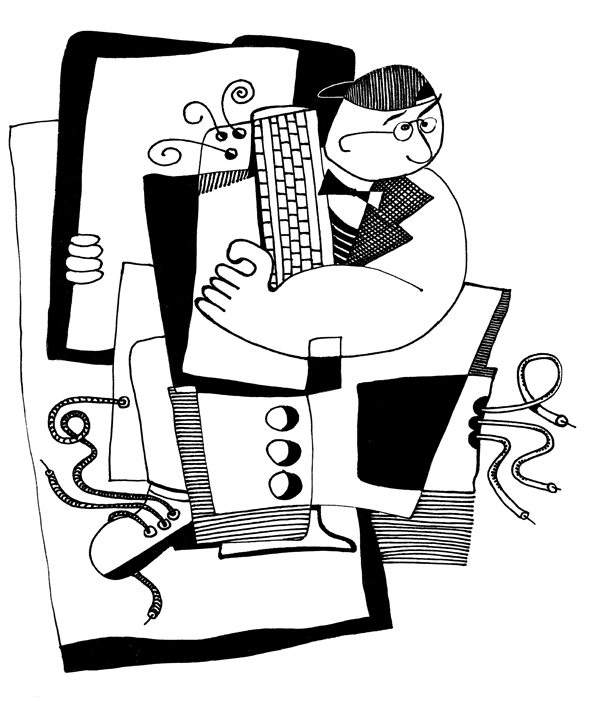
\includegraphics[scale=\FigScale]{cover.jpg}
\end{figure}

\bigskip

{\hfill \huge \AUTHOR}

\vspace*{\fill}
\end{center}

\end{titlepage}

\newpage

\begin{center}
\vspace*{\fill}
{\LARGE \TITLE}

\vspace*{\fill}

{\large \AUTHOR}

{\large \TT{<\EMAIL>}}
\vspace*{\fill}
\vfill

\ccbyncnd

\textcopyright 2013-2015, \AUTHOR. 

\RU{Это произведение доступно по лицензии Creative Commons «Attribution-NonCommercial-NoDerivs» 
(«Атрибуция~—~Некоммерческое использование~—~Без производных произведений») 3.0 Непортированная. 
Чтобы увидеть копию этой лицензии, посетите}
\EN{This work is licensed under the Creative Commons Attribution-NonCommercial-NoDerivs 3.0 Unported License. 
To view a copy of this license, visit} \url{http://creativecommons.org/licenses/by-nc-nd/3.0/}.

\RU{Версия этого текста}\EN{Text version} ({\large \today}).

\RU{Самая новая версия текста (а также англоязычная версия) доступна на сайте }%
\EN{The latest version (and Russian edition) of this text accessible at }%
\href{http://go.yurichev.com/17009}{beginners.re}.
\ifdefined\ebook
\RU{Версия формата A4 доступна там же.}
\EN{An A4-format version is also available.}
\else
\RU{Версия для электронных читалок так же доступна на сайте.}
\EN{An e-book reader version is also available.}
\fi

\ifx\LITE\undefined
\RU{Существует также LITE-версия (сокращенная вводная версия), предназначенная для быстрого ознакомления
с основами reverse engineering}%
\EN{There is also a LITE-version (introductory short version), intended for those who want a 
very quick introduction to the basics of reverse engineering}:
\href{http://go.yurichev.com/17358}{beginners.re}
\fi

\RU{Вы также можете подписаться на мой twitter для получения информации о новых версиях этого текста:
\TT{@yurichev}\footnote{\href{http://go.yurichev.com/17021}{twitter.com/yurichev}}, 
либо подписаться на список рассылки}%
\EN{You can also follow me on twitter to get information about updates of this text:
\TT{@yurichev}\footnote{\href{http://go.yurichev.com/17021}{twitter.com/yurichev}}
or to subscribe to the mailing list}%
\footnote{\href{http://go.yurichev.com/17020}{yurichev.com}}.

\RU{Обложка нарисована Андреем Нечаевским}\EN{The cover was made by Andy Nechaevsky}: \href{http://go.yurichev.com/17023}{facebook}.

\end{center}

\ifdefined\LITE
\begin{center}
\vspace*{\fill}

\Huge \RU{Внимание: это сокращенная LITE-версия}\EN{Warning: this is a shortened LITE-version}\ESph{}\PTBRph{}\PLph{}!
\normalsize

\bigskip
\bigskip
\bigskip

\Large
\RU{Она примерно в 6 раз короче полной версии (\textasciitilde{}150 страниц) и предназначена для тех,
кто хочет краткого введения в основы reverse engineering.
Здесь нет ничего о MIPS, ARM, OllyDBG, GCC, GDB, IDA, нет задач, примеров, \etc.}
\EN{It is approximately 6 times shorter than full version (\textasciitilde{}150 pages) and intended to those
who wants for very quick introduction to reverse engineering basics.
There are nothing about MIPS, ARM, OllyDBG, GCC, GDB, IDA, there are no exercises, examples, etc.}
\ESph{}\PTBRph{}\PLph{}
\normalsize

\bigskip
\bigskip
\bigskip

\RU{Если вам всё ещё интересен reverse engineering, полная версия книги всегда доступна на моем сайте}%
\EN{If you still interesting in reverse engineering, full version of the book is always available on my website}\ESph{}\PTBRph{}\PLph{}: 
\href{http://go.yurichev.com/17009}{beginners.re}.

\vspace*{\fill}
\vfill
\end{center}

\fi
%\begin{center}
\vspace*{\fill}

{\Huge \RU{Пожалуйста, заполните короткую анкету}\EN{Please take this short survey}!}
{\normalsize}

\bigskip
\bigskip
\bigskip

{\Large
\RU{Обратная связь для автора книги очень важна!}
\EN{Your feedback is extremely important to the author!}}

\bigskip
\bigskip
\bigskip

\url{http://beginners.re/survey.html}

\bigskip
\bigskip
\bigskip

\vspace*{\fill}
\vfill
\end{center}


\ifx\LITE\undefined
\shorttoc{\RU{Краткое оглавление}\EN{Abridged contents}\PTBRph{}\ESph{}\PLph{}}{-1} % Only sections
\fi
\tableofcontents
\cleardoublepage

\cleardoublepage
\section*{\RU{Предисловие}\EN{Preface}\PTBRph{}\ESph{}\PLph{}}

\iffalse
\RU{Здесь (будет) немного моих заметок о \gls{reverse engineering} на русском языке для начинающих, 
для тех кто хочет научиться понимать создаваемый \CCpp компиляторами код для x86 (коего, 
практически, больше всего остального) и ARM.}
\EN{Here are some of my notes in English for beginners in \gls{reverse engineering}
who would like to learn to understand x86 (which accounts for almost
all executable software in the world) and ARM code created by \CCpp compilers.}
\fi

\RU{У термина \q{\gls{reverse engineering}} несколько популярных значений:
1) исследование скомпилированных
программ; 2) сканирование трехмерной модели для последующего копирования;
3) восстановление структуры СУБД. Настоящий сборник заметок
связан с первым значением.}
\EN{There are several popular meanings of the term \q{\gls{reverse engineering}}:
1) The reverse engineering of software: researching compiled programs;
2) The scanning of 3D structures and the subsequent digital manipulation required order to duplicate them;
3) recreating \ac{DBMS} structure.
This book is about the first meaning.}

\ifx\LITE\undefined
\subsection*{\RU{Рассмотренные темы}\EN{Topics discussed in-depth}\PTBRph{}\ESph{}\PLph{}}

x86/x64, ARM/ARM64, MIPS, Java/JVM.

\subsection*{\RU{Затронутые темы}\EN{Topics touched upon}\PTBRph{}\ESph{}\PLph{}}

\oracle (\myref{oracle}),
Itanium (\myref{itanium}),
\RU{донглы для защиты от копирования}\EN{copy-protection dongles} (\myref{dongles}), 
LD\_PRELOAD (\myref{ld_preload}),
\RU{переполнение стека}\EN{stack overflow}, 
\ac{ELF},
\RU{формат файла PE в win32}\EN{win32 PE file format} (\myref{win32_pe}),
x86-64 (\myref{x86-64}),
\RU{критические секции}\EN{critical sections} (\myref{critical_sections}),
\RU{системные вызовы}\EN{syscalls} (\myref{syscalls}), 
\ac{TLS},
\RU{адресно-независимый код}\EN{position-independent code} (\ac{PIC}) (\myref{sec:PIC}), 
profile-guided optimization (\myref{PGO}),
C++ STL (\myref{cpp_STL}),
OpenMP (\myref{openmp}),
SEH (\myref{sec:SEH}).
\fi

\subsection*{\RU{Об авторе}\EN{About the author}\PTBRph{}\ESph{}\PLph{}}

\begin{tabularx}{\textwidth}{ l X }

\raisebox{-\totalheight}{
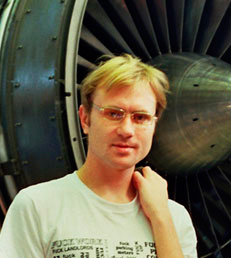
\includegraphics[scale=0.60]{Dennis_Yurichev.jpg}
}

&
\RU{Денис Юричев~--- опытный reverse engineer и программист.}%
\EN{Dennis Yurichev is an experienced reverse engineer and programmer.}
\EN{He can be contacted by email:}%
\RU{С ним можно контактировать по емейлу:} \textbf{\EMAIL{}}, 
\EN{or on Skype:}\RU{или по Skype:} \textbf{dennis.yurichev}.

% FIXME: no link. \tablefootnote doesn't work
\end{tabularx}

% subsections:
\subsection*{\RU{Отзывы о книге}\EN{Praise for} \IT{\TITLE}}

\begin{itemize}
% expanded URLs to make it more robust for printouts. In electronic editions people will click anyway, so tracking will keep working
\item \q{It's very well done .. and for free .. amazing.}\footnote{\href{http://go.yurichev.com/17095}{twitter.com/daniel\_bilar/status/436578617221742593}} Daniel Bilar, Siege Technologies, LLC.

\item \q{... excellent and free}\footnote{\href{http://go.yurichev.com/17096}{twitter.com/petefinnigan/status/400551705797869568}} Pete Finnigan, \RU{гуру по безопасности }\oracle\EN{ security guru}.

\item \q{... book is interesting, great job!} Michael Sikorski, \RU{автор книги}\EN{author of} \IT{Practical Malware Analysis: The Hands-On Guide to Dissecting Malicious Software}.

\item \q{... my compliments for the very nice tutorial!} Herbert Bos, \RU{профессор университета}\EN{full professor at the} Vrije Universiteit Amsterdam, \RU{соавтор}\EN{co-author of} \IT{Modern Operating Systems (4th Edition)}.

\item \q{... It is amazing and unbelievable.} Luis Rocha, CISSP / ISSAP, Technical Manager, Network \& Information Security at Verizon Business.

\item \q{Thanks for the great work and your book.} Joris van de Vis, \RU{специалист по} SAP Netweaver \& Security\EN{ specialist}.

\item \q{... reasonable intro to some of the techniques.}\footnote{\href{http://go.yurichev.com/17099}{reddit}} Mike Stay, \RU{преподаватель в}\EN{teacher at the} Federal Law Enforcement Training Center, Georgia, US.

\item \q{I love this book! I have several students reading it at the moment, plan to use it in graduate course.}\footnote{\href{http://go.yurichev.com/17097}{twitter.com/sergeybratus/status/505590326560833536}} \EN{Sergey Bratus}\RU{Сергей Братусь}, Research Assistant Professor \RU{в отделе Computer Science}\EN{at the Computer Science Department} \RU{в}\EN{at} Dartmouth College

\item \q{Dennis @Yurichev has published an impressive (and free!) book on reverse engineering}\footnote{\href{http://go.yurichev.com/17098}{twitter.com/TanelPoder/status/524668104065159169}} Tanel Poder, \EN{Oracle RDBMS performance tuning expert}\RU{эксперт по настройке производительности Oracle RDBMS}.

\item \q{This book is some kind of Wikipedia to beginners...} Archer, Chinese Translator, IT Security Researcher.

\RU{\item \q{Прочел Вашу книгу~--- отличная работа, рекомендую на своих курсах студентам
в качестве учебного пособия}. Николай Ильин, преподаватель в ФТИ НТУУ \q{КПИ} и DefCon-UA}
\end{itemize}


\subsection*{\RU{Благодарности}\EN{Thanks}\PTBRph{}\ESph{}\PLph{}}

\RU{Тем, кто много помогал мне отвечая на массу вопросов}\EN{For patiently answering all my questions}:
\HERMIT, \RU{Слава \q{Avid} Казаков}\EN{Slava \q{Avid} Kazakov}.

\RU{Тем, кто присылал замечания об ошибках и неточностях}\EN{For sending me notes
about mistakes and inaccuracies}:
\RU{Станислав \q{Beaver} Бобрицкий, Александр Лысенко}%
\EN{Stanislav \q{Beaver} Bobrytskyy, Alexander Lysenko}, Shell Rocket, Zhu Ruijin, Changmin Heo.

\RU{Просто помогали разными способами}\EN{For helping me in other ways}:
\RU{Андрей Зубинский}\EN{Andrew Zubinski}, 
Arnaud Patard (rtp \RU{на}\EN{on} \#debian-arm IRC),
\EN{Aliaksandr Autayeu}\RU{Александр Автаев}.

\RU{Переводчикам на китайский язык}\EN{For translating the book into Simplified Chinese}: Antiy Labs (\href{http://antiy.cn}{antiy.cn}) \AndENRU Archer.

\RU{Переводчику на корейский язык}\EN{For translating the book into Korean}: Byungho Min.

\RU{Корректорам}\EN{For proofreading}:
\RU{Александр \q{Lstar} Черненький}\EN{Alexander \q{Lstar} Chernenkiy},
\RU{Владимир Ботов}\EN{Vladimir Botov},
\RU{Андрей Бражук}\EN{Andrei Brazhuk},
\RU{Марк}\EN{Mark} ``Logxen'' \RU{Купер}\EN{Cooper},
Yuan Jochen Kang, Mal Malakov, Lewis Porter, Jarle Thorsen.

\RU{Васил Колев сделал очень много исправлений и указал на многие ошибки.}
\EN{Vasil Kolev did a great amount of work in proofreading and correcting many mistakes.}

\RU{За иллюстрации и обложку: Андрей Нечаевский.}\EN{For illustrations and cover art: Andy Nechaevsky.}

\RU{И ещё всем тем на github.com кто присылал замечания и исправления.}
\EN{Thanks also to all the folks on github.com who have contributed notes and corrections.}

\RU{Было использовано множество пакетов \LaTeX. Их авторов я также хотел бы поблагодарить.}
\EN{Many \LaTeX\ packages were used: I would like to thank the authors as well.}

\subsubsection*{\RU{Жертвователи}\EN{Donors}}

\EN{Those who supported me during the time when I wrote significant part of the book:}%
\RU{Те, кто поддерживал меня во время написании этой книги:}

2 * Oleg Vygovsky (50+100 UAH), 
Daniel Bilar ($\$$50), 
James Truscott ($\$$4.5),
Luis Rocha ($\$$63), 
Joris van de Vis ($\$$127), 
Richard S Shultz ($\$$20), 
Jang Minchang ($\$$20), 
Shade Atlas (5 AUD), 
Yao Xiao ($\$$10),
Pawel Szczur (40 CHF), 
Justin Simms ($\$$20), 
Shawn the R0ck ($\$$27), 
Ki Chan Ahn ($\$$50), 
Triop AB (100 SEK), 
Ange Albertini (\euro{}10+50),
Sergey Lukianov (300 RUR), 
Ludvig Gislason (200 SEK), 
Gérard Labadie (\euro{}40), 
Sergey Volchkov (10 AUD),
Vankayala Vigneswararao ($\$$50),
Philippe Teuwen ($\$$4),
Martin Haeberli ($\$$10),
Victor Cazacov (\euro{}5),
Tobias Sturzenegger (10 CHF),
Sonny Thai ($\$$15),
Bayna AlZaabi ($\$$75),
Redfive B.V. (\euro{}25),
Joona Oskari Heikkilä (\euro{}5),
Marshall Bishop ($\$$50),
Nicolas Werner (\euro{}12),
Jeremy Brown ($\$$100),
Alexandre Borges ($\$$25),
Vladimir Dikovski (\euro{}50),
Jiarui Hong (100.00 SEK),
Jim Di (500 RUR),
Tan Vincent ($\$$30),
Sri Harsha Kandrakota (10 AUD),
Pillay Harish (10 SGD),
Timur Valiev (230 RUR),
Carlos Garcia Prado (\euro{}10),
Salikov Alexander (500 RUR),
Oliver Whitehouse (30 GBP),
Katy Moe ($\$$14),
Maxim Dyakonov ($\$$3),
Sebastian Aguilera (\euro{}20),
Hans-Martin Münch (\euro{}15),
Jarle Thorsen (100 NOK),
Vitaly Osipov ($\$$100),
Yuri Romanov (1000 RUR),
Aliaksandr Autayeu (\euro{}10),
Tudor Azoitei ($\$$40),
Z0vsky (\euro{}10),
Yu Dai ($\$$10). 

\RU{Огромное спасибо каждому!}\EN{Thanks a lot to every donor!}

% subsections
\subsection*{mini-\RU{ЧаВО}\EN{FAQ}}

\newcommand{\HACKINGMdURL}{https://github.com/dennis714/RE-for-beginners/blob/master/HACKING.md}
\newcommand{\FNURLREDDIT}{\footnote{\href{http://go.yurichev.com/17027}{reddit.com/r/ReverseEngineering/}}}

Q: \EN{Why should one learn assembly language these days?}\RU{Зачем в наше время нужно изучать язык ассемблера?}\\
A: \EN{Unless you are an \ac{OS} developer, you probably don't need to code in assembly\EMDASH{}modern compilers 
are much better at performing optimizations than humans}
\RU{Если вы не разработчик \ac{OS}, вам наверное не нужно писать на ассемблере:
современные компиляторы оптимизируют код намного лучше человека}%
\footnote{\RU{Очень хороший текст на эту тему}\EN{A very good text about this topic}: \cite{AgnerFog}}.
\EN{Also, modern \ac{CPU}s are very complex devices and assembly knowledge doesn't really help one to understand their internals.}
\RU{К тому же, современные \ac{CPU} это крайне сложные устройства и знание ассемблера вряд ли
поможет узнать их внутренности.}
\EN{That being said, there are at least two areas where a good understanding of assembly can be helpful: 
First and foremost, security/malware research. It is also a good way to gain a better understanding of your compiled code whilst debugging.}
\RU{Но все-таки остается по крайней мере две области, где знание ассемблера может хорошо
помочь:
1) исследование malware (\IT{зловредов}) с целью анализа; 2) лучшее понимание
вашего скомпилированного кода в процессе отладки.}
\EN{This book is therefore intended for those who want to understand assembly language rather 
than to code in it, which is why there are many examples of compiler output contained within.}
\RU{Таким образом, эта книга предназначена для тех, кто хочет скорее понимать ассемблер,
нежели писать на нем, и вот почему здесь масса примеров, связанных с результатами
работы компиляторов.}\\
\\
Q: \RU{Я кликнул на ссылку внутри PDF-документа, как теперь вернуться назад?}\EN{I clicked on a hyperlink inside a PDF-document, how do I go back?}\\
A: \RU{В Adobe Acrobat Reader нажмите сочетание Alt+LeftArrow.}\EN{In Adobe Acrobat Reader click Alt+LeftArrow.}\\
\\
\ifx\LITE\undefined
Q: \RU{Ваша книга слишком большая! Нет ли чего покороче?}\EN{Your book is huge! Is there anything shorter?}\\
A: \RU{Есть сокращенная lite-версия}\EN{There is shortened, lite version found here}: \url{http://beginners.re/\#lite}.\\
\\
\fi
Q: \RU{Я не могу понять, стоит ли мне заниматься reverse engineering-ом}\EN{I'm not sure if I should try to learn reverse engineering or not}.\\
A: \RU{Наверное, среднее время для освоения сокращенной LITE-версии\EMDASH{}1-2 месяца.}%
\EN{Perhaps, the average time to become familiar with the contents of the shortened LITE-version is 1-2 month(s).}\\
\\
Q: \RU{Могу ли я распечатать эту книгу? Использовать её для обучения?}\EN{May I print this book? Use it for teaching?}\\
A: \RU{Конечно, поэтому книга и лицензирована под лицензией Creative Commons.}\EN{Of course! That's why the book is licensed under the Creative Commons license.}
\EN{One might also want to build one's own version of book\EMDASH{}read \href{\HACKINGMdURL}{here} to find out more.}
\RU{Кто-то может захотеть скомпилировать свою собственную версию книги, читайте \href{\HACKINGMdURL}{здесь} об этом.}\\
\\
Q: \RU{Я хочу перевести вашу книгу на другой язык}\EN{I want to translate your book to some other language}.\\
A: \RU{Прочитайте}\EN{Read} \href{https://github.com/dennis714/RE-for-beginners/blob/master/Translation.md}{\RU{мою заметку для переводчиков}\EN{my note to translators}}.\\
\\
Q: \RU{Как можно найти работу reverse engineer-а}\EN{How does one get a job in reverse engineering}? \\
A: \RU{На reddit, посвященному RE\FNURLREDDIT, время от времени бывают hiring thread}
\EN{There are hiring threads that appear from time to time on reddit, devoted to RE\FNURLREDDIT}
(\href{http://go.yurichev.com/17333}{2013 Q3}, 
\href{http://go.yurichev.com/17334}{2014}).
\RU{Посмотрите там}\EN{Try looking there}.
\EN{A somewhat related hiring thread can be found in the \q{netsec} subreddit}\RU{В смежном субреддите \q{netsec} имеется похожий тред}:
\href{http://go.yurichev.com/17335}{2014 Q2}.\\
\\
\RU{Q: Куда пойти учиться в Украине?\\
A: \href{http://go.yurichev.com/17336}{НТУУ \q{КПИ}: \q{Аналіз програмного коду та бінарних вразливостей}};
\href{http://go.yurichev.com/17337}{факультативы}.\\
\\}
Q: \EN{I have a question}\RU{У меня есть вопрос}...\\
A: \EN{Send it to me by email}\RU{Напишите мне его емейлом} (\EMAIL).


\ifdefined\ebook
\RU{Это версия формата A5 для электронных читалок}\EN{This is the A5-format version for e-book readers}. 
\RU{Хотя, тут всё то же самое, но иллюстрации уменьшены и не очень хорошо читаемы}
\EN{Although the content is mostly the same, the illustrations are resized and probably not readable}. 
\EN{You may try to change scale in your e-book reader.}
\RU{Вы можете попробовать изменить масштаб в вашей читалке.}
\RU{Так или иначе, вы всегда можете посмотреть их в версии формата A4 здесь}
\EN{Otherwise, you can always view them in the A4-format version here}: \href{http://go.yurichev.com/17009}{beginners.re}.
\fi

% {\RU{Целевая аудитория}\EN{Target audience}}

\subsection*{\RU{О переводе на корейский язык}\EN{About the Korean translation}\PTBRph{}\ESph{}\PLph{}}

\EN{In January 2015, the Acorn publishing company (\href{http://www.acornpub.co.kr}{www.acornpub.co.kr}) in South Korea did a huge amount of work in translating and publishing 
my book (as it was in August 2014) into Korean.}
\RU{В январе 2015, издательство Acorn в Южной Корее сделало много работы в переводе 
и издании моей книги (по состоянию на август 2014) на корейский язык.}

\RU{Она теперь доступна на}\EN{It's now available at} 
\href{http://go.yurichev.com/17343}{\EN{their website}\RU{их сайте}}.

\iffalse
\begin{figure}[H]
\centering
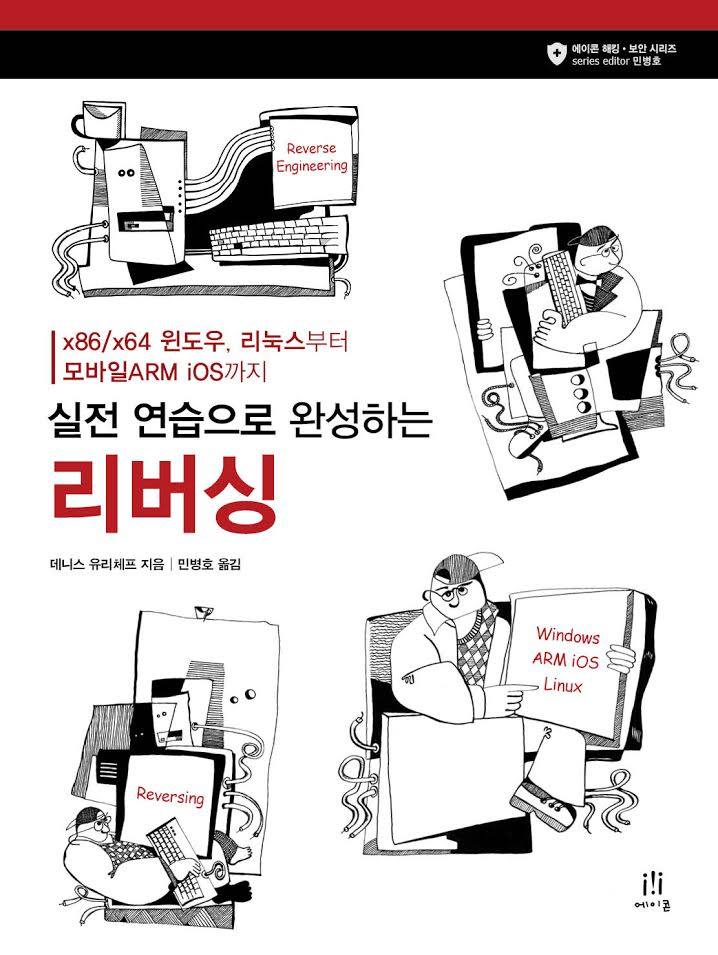
\includegraphics[scale=0.3]{acorn_cover.jpg}
\end{figure}
\fi

\RU{Переводил}\EN{The translator is} Byungho Min (\href{http://go.yurichev.com/17344}{twitter/tais9}).

\EN{The cover art was done by my artistic friend, Andy Nechaevsky}
\RU{Обложку нарисовал мой хороший знакомый художник Андрей Нечаевский}: 
\href{http://go.yurichev.com/17023}{facebook/andydinka}.

\RU{Они также имеют права на издании книги на корейском языке.}
\EN{They also hold the copyright to the Korean translation.}

\RU{Так что если вы хотите иметь \IT{настоящую} книгу на полке на корейском языке и
хотите поддержать мою работу, вы можете купить её.}
\EN{So, if you want to have a \IT{real} book on your shelf in Korean and 
want to support my work, it is now available for purchase.}


\mainmatter

\ifx\LITE\undefined
\def\IncludeGCC{}
\def\IncludeARM{}
\def\IncludeOlly{}
\def\IncludeGDB{}
\def\IncludeExercises{}
\def\IncludeHiew{}
\def\IncludeCPP{}
\def\IncludeMIPS{}
\def\IncludeJavaAndNET{}
\def\IncludeOracle{}
\def\IncludeDongles{}
\def\IncludeItanium{}
\def\IncludeMSDOS{}
\def\IncludeWinSixteen{}

\fi

% only parts here!
%FIXME: requires PTBR and ES revision (dbmussi)
\part{\RU{Образцы кода}\EN{Code patterns}\PTBR{Padrões de código}\ES{Patrones de código}}

\RU{\epigraph{Всё познается в сравнении}{Автор неизвестен}}
\EN{\epigraph{Everything is comprehended in comparison}{Author unknown}}
\PTBR{\epigraph{Tudo é relativo}{Autor desconhecido}}
\ES{\epigraph{Todo es relativo}{Autor desconocido}}
% FIXME: english sentence added. (dbmussi) 
% not sure it's correct. (yurichev)
% this is popular Russian proverb and is close to "everything is comprehended in comparison", but the source is lost, however, 
% it's traditionally attributed to all sorts of philosophers..
% I don't know exact analgoue in English language, but OK, let it be so.

\RU{Когда автор этой книги учил Си, а затем \Cpp, он просто писал небольшие фрагменты кода, компилировал и смотрел, что 
получилось на ассемблере. Так было намного проще понять%
\footnote{Честно говоря, он и до сих пор так делаю, когда не понимают, как работает некий код.}.
Он делал это такое количество раз, что связь между кодом на \CCpp и тем, что генерирует компилятор, вбилась в его подсознание достаточно глубоко.
После этого не трудно, глядя на код на ассемблере, сразу в общих чертах понимать, что там было написано на Си. 
Возможно это поможет кому-то ещё.}
\EN{When the author of this book first started learning C and, later, \Cpp, he used to write small pieces of code, compile them, 
and then look at the assembly language output. This made it very easy for him to understand what was going on in the code that he had written.
\footnote{In fact, he still does it when he can't understand what a particular bit of code does.}. 
He did it so many times that the relationship between the \CCpp code and what the compiler produced was imprinted deeply in his mind. 
It's easy to imagine instantly a rough outline of C code's appearance and function. 
Perhaps this technique could be helpful for others.}
\PTBR{Quando o autor deste livro começou a aprender C e, mais tarde, \Cpp, ele costumava escrever pequenos pedaços de código, compilá-los, 
e então olhar a saída em linguagem assembly. Isso tornou muito fácil para ele entender o que estava acontecendo no código que ele tinha escrito.
\footnote{Na verdade, ele ainda faz isso quando não consegue entender o que faz um determinado pedaço de código.}. 
Ele fez isso tantas vezes que o relacionamento entre o código \CCpp code e o que o compilador produzia ficou registrado profundamente em sua mente. 
É fácil imaginar de imediato um esboço da aparência e função do código C. 
Talvez essa técnica poderia ser útil para mais alguém.}
\ES{Cuando el autor de este libro comenzó a aprender C y, más tarde, \Cpp, él solía escribir pequeños trozos de código, compilarlos, 
y luego ver los resultados en lenguaje assembly. Esto lo hizo muy fácil para él entender lo que estaba pasando en el código que había escrito.
\footnote{De hecho, todavia lo hace cuando no puede entender lo que hace una determinada pieza de código.}. 
Él lo hizo tantas veces que la relación entre el código \CCpp y lo que el compilador producido se imprimió profundamente en su mente. 
És fácil imaginar al instante un esbozo de la aparencia y función del código C. 
Quizás esta técnica podría ser útil para otra persona.}

%
%\RU{Здесь много примеров и для x86/x64 и для ARM}\EN{There are a lot of examples for both x86/x64 
%and ARM}.\PTBR{Há uma série de exemplos para ambos x86/x64 e ARM}.\ES{Hay una serie de ejemplos, tanto para x86/x64 y ARM} 
%\RU{Те, кто уже хорошо знаком с одной из архитектур, могут легко пролистывать страницы}
%\EN{Those who already familiar with one of architectures, may freely skim over pages}.
%\PTBR{Aqueles já familiarizados com alguma das arquiteturas, pode ler superficialmente as próximas páginas}.
%\ES{Los que ya están familiarizados con alguna de las arquitecturas, pueden leer superficialmente las páginas siguientes}.

\RU{Иногда здесь используются достаточно древние компиляторы, чтобы получить самый короткий (или простой) фрагмент кода.}%
\EN{Sometimes ancient compilers are used here, in order to get the shortest (or simplest) possible code snippet.}
\PTBR{Em determinadas partes foram usados aqui compiladores muito antigos, para se obter o menor (ou mais simples) snippet possível.}
\ES{En ciertas partes, se han empleado aquí compiladores muy antiguas, con el fin de obtener lo mas corta (o simple) posible snippet.}
\

\ifdefined\IncludeExercises
\section*{\Exercises}

\RU{Когда автор этой книги учил ассемблер, он также часто компилировал короткие функции на Си и затем постепенно 
переписывал их на ассемблер, с целью получить как можно более короткий код.}%
\EN{When the author of this book studied assembly language, he also often compiled small C-functions and then rewrote
them gradually to assembly, trying to make their code as short as possible.}
\PTBR{Quando o autor deste livro estudou a linguagem assembly, ele também frequentemente compilava pequenas funções em C e então as reescrevia gradualmente em assembly, tentando fazer seu código o menor possível.}
\ES{Cuando el autor de este libro estudió la lenguaje assembly, también con frecuencia compilaba pequeñas funciones en C, y reescribia gradualmente en assembly, tratando de hacer el código lo más pequeño posible}
\RU{Наверное, этим не стоит заниматься в наше время на практике (потому что конкурировать с современными
компиляторами в плане эффективности очень трудно), но это очень хороший способ разобраться в ассемблере
лучше.}%
\EN{This probably is not worth doing in real-world scenarios today, 
because it's hard to compete with modern compilers in terms of efficiency. It is, however, a very good way to gain a better understanding of assembly.}
\PTBR{Provavelmente não vale mais à pena fazer isso em cenários reais atualmente, 
porque é difícil competir com os compiladores modernos em termos de eficiência. É, no entanto, uma forma muito boa de obter um melhor entendimento de assembly.}
\ES{Probablemente no vale la pena hacer esto en escenarios reales actualmente, 
porque es dificil competir con los compiladores modernos en términos de eficiencia. Es, sin embargo, una muy buena manera de obtener una mejor compreensión de la assembly}

\RU{Так что вы можете взять любой фрагмент кода на ассемблере в этой книге и постараться сделать его короче.}%
\EN{Feel free, therefore, to take any assembly code from this book and try to make it shorter.}
\PTBR{Sinta-se livre, portanto, para pegar qualquer código assembly deste livro e tentar torná-lo menor.}
\ES{Siéntase libre, por lo tanto, para tomar cualquier código de este libro y tratar de hacerlo más pequeño.}
\RU{Но не забывайте о тестировании своих результатов.}%
\EN{However, don't forget to test what you have written.}
\PTBR{No entanto, não esqueça de testar o que você tiver escrito.}
\ES{Sin embargo, no se olvide de probar lo que has escrito.}
\fi

% rewrote to show that debug\release and optimisations levels are orthogonal concepts.
\section*{\RU{Уровни оптимизации и отладочная информация}\EN{Optimization levels and debug information}\PTBR{Níveis de otimização e informação de depuração}\ES{Níveles de optimización y la información de depuración}}

\RU{Исходный код можно компилировать различными компиляторами с различными уровнями оптимизации.
В типичном компиляторе этих уровней около трёх, где нулевой уровень~--- отключить оптимизацию.
Различают также направления оптимизации кода по размеру и по скорости.}
\EN{Source code can be compiled by different compilers with various optimization levels.
A typical compiler has about three such levels, where level zero means disable optimization.
Optimization can also be targeted towards code size or code speed.}
\PTBR{O código-fonte pode ser compilado por diferentes compiladores com vários níveis de otimização.
Um compilador típico tem cerca de três destes níveis, onde o nível zero significa desativar a otimização.
A otimização também pode ser direcionada para o tamanho do código ou para a velocidade do código.}
\ES{El código fuente puede ser compilado por diferentes compiladores com varios niveles de optimización.
Un compilador típico tiene alredor de tres de esos niveles, donde el nivel cero significa desactivar la optimización.
La optimización también puede dirigirse hacia el tamaño del código o la velocidad de código.}

\RU{Неоптимизирующий компилятор работает быстрее, генерирует более понятный (хотя и более объемный) код.
Оптимизирующий компилятор работает медленнее и старается сгенерировать более быстрый (хотя и не обязательно краткий) код.}
\EN{A non-optimizing compiler is faster and produces more understandable (albeit verbose) code,
whereas an optimizing compiler is slower and tries to produce code that runs faster (but is not necessarily more compact).}
\PTBR{Um compilador sem otimização é mais rápido e produz código mais inteligível (embora maior),
enquanto que um compilador com otimização é mais lento e tenta produzir um código que execute mais rápido (mas não é necessariamente mais compacto).}
\ES{Un compilador sin optimización es más rápido y produce código más inteligible (aunque más grande), 
mientras un compilador con optimización es más lento y trata de producir un código que corre más rápido (pero no necesariamente más compacto).}

\RU{Наряду с уровнями и направлениями оптимизации компилятор может включать в конечный файл отладочную информацию,
производя таким образом код, который легче отлаживать.}
\EN{In addition to optimization levels and direction, a compiler can include in the resulting file some debug information,
thus producing code for easy debugging.}
\PTBR{Além dos níveis e direcionamento da otimização, o compilador pode incluir no arquivo resultante algumas informações de depuração, produzindo assim código para fácil depuração.}
\ES{Además de los niveles y dirección de la otimización, el compilador puede incluir informaciones de depuración en el archivo resultante, produciendo así código para fácil depuración.}

\RU{Одна очень важная черта отладочного кода в том, что он может содержать
связи между каждой строкой в исходном коде и адресом в машинном коде.}
\EN{One of the important features of the ´debug' code is that it might contain links
between each line of the source code and the respective machine code addresses.}
\PTBR{Uma das características importantes do código de ´debug' é que ele pode conter 
ligações entre cada linha do código-fonte e os respectivos endereços de código de máquina.}
\ES{Una de los características importantes del código de ´debug' és que puede contener enlaces entre
cada línea del código fuente y las direcciones de código de máquina respectivos.}
\RU{Оптимизирующие компиляторы обычно генерируют код, где целые строки из исходного кода
могут быть оптимизированы и не присутствовать в итоговом машинном коде.}
\EN{Optimizing compilers, on the other hand, tend to produce output where entire lines of source code
can be optimized away and thus not even be present in the resulting machine code.}
\PTBR{Compiladores com otimização, por outro lado, tendem a produzir uma saída onde linhas inteiras de código-fonte podem ser otimizadas a ponto de serem removidas e portanto não estarem presentes no código de máquina resultante.}
\ES{Compiladores con optimización, por otro lado, tienden a producir una salida donde líneas enteras de código fuente pueden ser optimizados al punto de ser eliminados y por consiguiente no estar presentes en el código de máquina resultante.}

\RU{Практикующий reverse engineer обычно сталкивается с обоими версиями, потому что некоторые разработчики
включают оптимизацию, некоторые другие\EMDASH{}нет. Вот почему мы постараемся поработать с примерами для обоих версий.}
\EN{Reverse engineers can encounter either version, simply because some developers turn on the compiler's optimization flags and others do not. 
Because of this, we'll try to work on examples of both debug and release versions of the code featured in this book, where possible.}
\PTBR{Engenheiros Reversos podem encontrar ambas as versões, simplesmente porque alguns desenvolvedores ativam as flags de otimização do compilador e outros não ativam. 
Por causa disso, nós tentaremos trabalhar em exemplos de ambas as versões de debug e release do código destacado neste livro, onde possível.}
\ES{Ingenieros Inversos pueden encontrar ambas versiones, simplesmente porque alguns desarrolladores activan los flags de optimización del compilador, y otros no activan. 
Debido a esto, vamos a tratar de trabajar con ejemplos de ambas versiones de debug y release del código resaltado en este libro, cuando sea posible.}

\chapter{\RU{Краткое введение в CPU}\EN{A short introduction to the CPU}\PTBR{Uma breve introdução à CPU}\ES{Una breve introducción a la CPU}}

\EN{The}\PTBR{A}\ES{La} \ac{CPU} \RU{это устройство исполняющее все программы}\EN{is the device that executes the machine code a program consists of}\PTBR{é o dispositivo que executa o código de máquina que consiste num programa}\ES{es el dispositivo que ejecuta el código de máquina que constituye un programa}.

\textbf{\RU{Немного терминологии}\EN{A short glossary}\PTBR{Um pequeno glossário}\ES{Un breve glosario}:}

\begin{description}
\item[\RU{Инструкция}\EN{Instruction}\PTBR{Instrução}\ES{Instrucción}]: \RU{примитивная команда}\EN{A primitive}\PTBR{Um primitivo}\ES{Una primitiva}
	\ac{CPU}\RU{.} \EN{command.}\PTBR{comando.}\ES{comando.}
\RU{Простейшие примеры: перемещение между регистрами, работа с памятью, примитивные арифметические операции}%
\EN{The simplest examples include: moving data between registers, working with memory, primitive arithmetic operations}
\PTBR{Os exemplos mais simples incluem: mover dados entre registradores, trabalhar com a memória, operações aritiméticas primitivas}
\ES{Los ejemplos más simples incluyen: mover datos entre registros, trabajar con la memoria, operaciones aritméticas primitivas}.
\RU{Как правило, каждый}\EN{As a rule, each}\PTBR{Como regra geral, cada}\ES{Como regla general, cada} \ac{CPU} \RU{имеет свой набор инструкций}\EN{has its own instruction set architecture}\PTBR{tem seu próprio conjunto de instruções}\ES{tiene su proprio conjunto de instrucciones} 
(\ac{ISA}).

\item[\RU{Машинный код}\EN{Machine code}]: \RU{код понимаемый}\EN{Code that the}\PTBR{Código que a}\ES{Código que la} \ac{CPU}\EN{ directly processes}\PTBR{ processa diretamente}\ES{ procesa directamente}. 
\RU{Каждая инструкция обычно кодируется несколькими байтами}\EN{Each instruction is usually encoded by several bytes}\PTBR{Cada instrução é normalmente codificada em vários bytes}\ES{Cada instrucción generalmente se codifica por vários bytes}.

\item[\RU{Язык ассемблера}\EN{Assembly language}\PTBR{Linguagem assembly}\ES{Lenguaje assembly}]: 
\RU{машинный код плюс некоторые расширения, призванные облегчить труд программиста: макросы, имена, \etc.}
\EN{Mnemonic code and some extensions like macros that are intended to make a programmer's life easier.}
\PTBR{Código mnemônico e algumas extensões como macros que têm a finalidade de facilitar a vida do programamdor.}
\ES{Código mnemónico y algunas extensiones como macros que destinados a hacer la vida del programador más fácil.}

\item[\RU{Регистр CPU}\EN{CPU register}\PTBR{Registradores da CPU}\ES{Registros de la CPU}]: 
\RU{Каждый}\EN{Each}\PTBR{Cada}\ES{Cada} \ac{CPU} \RU{имеет некоторый фиксированный набор регистров общего назначения}\EN{has a fixed set of general purpose registers}\PTBR{tem um conjunto fixo de registradores de propósito geral}\ES{tiene un conjunto fijo de registros de propósito general} (\ac{GPR}).
$\approx 8$ \InENRU x86, $\approx 16$ \InENRU x86-64, $\approx 16$ \InENRU ARM.
\RU{Проще всего понимать регистр как временную переменную без типа}%
\EN{The easiest way to understand a register is to think of it as an untyped temporary variable}
\PTBR{A forma mais fácil de entender um registrador é pensar nele como uma variável temporária não tipada}
\ES{La forma más fácil de entender un registro es pensar en ello como una variable temporal sin tipo}.
\RU{Можно представить, что вы пишете на \ac{PL} высокого уровня и у вас только 8 переменных шириной 32 (или 64) бита}%
\EN{Imagine if you were working with a high-level \ac{PL} and could only use eight 32-bit (or 64-bit) variables}
\PTBR{Imagine que você estivesse trabalhando com uma \ac{PL} de alto nível e pudesse usar apenas oito variáveis de 32-bit (ou de 64-bit)}
\ES{Imagine si estuviera trabajando con una \ac{PL} de alto nivel y sólo podría utilizar ocho variables de 32-bit (o de 64-bit)}.
\RU{Можно сделать очень много используя только их}\EN{Yet a lot can be done using just these}\PTBR{No entanto, muito ainda pode ser feito usando apenas eles}\ES{Sin embargo mucho se puede hacer usando sólo estos}!
\end{description}

\RU{Откуда взялась разница между машинным кодом и \ac{PL} высокого уровня?
Ответ в том, что люди и \ac{CPU}-ы отличаются друг от друга\EMDASH{}}
\EN{One might wonder why there needs to be a difference between machine code and a \ac{PL}.
The answer lies in the fact that humans and \ac{CPU}s are not alike\EMDASH{}}
\PTBR{Alguém poderia perguntar por que é preciso haver diferença entre código de máquina e uma \ac{PL} de alto nível.
A resposta reside no fato de que humanos e \ac{CPU}s não são iguais\EMDASH{}}
\ES{Uno podría perguntarse por qué es necessário que haya diferencia entre el código de la máquina y una lenguaje de programación de alto nivel.
La respuesta está en el hecho de que los seres humanos y CPUs no son iguales\EMDASH{}}.
\RU{Человеку проще писать на \ac{PL} высокого уровня вроде \CCpp, Java, Python, 
а \ac{CPU} проще работать с абстракциями куда более низкого уровня}%
\EN{It is much easier for humans to use a high-level \ac{PL} like \CCpp, Java, Python, etc., 
but it is easier for a \ac{CPU} to use a much lower level of abstraction}
\PTBR{É muito mais fácil para os humanos usar uma \ac{PL} de alto nível como \CCpp, Java, Python, etc.,
mas é muito mais fácil para a \ac{CPU} usar um nível de abstração muito menor}
\ES{És mucho más fácil para los humanos utilizar un \ac{PL} de alto nivel como \CCpp, Java, Python, etc., 
pero és más fácil para una \ac{CPU} utilizar un nivel mucho más bajo de abstración}.
\RU{Возможно, можно было бы придумать \ac{CPU} исполняющий код \ac{PL} высокого уровня, но он был бы значительно сложнее, чем те, что мы имеем сегодня}
\EN{Perhaps it would be possible to invent a \ac{CPU} that can execute high-level \ac{PL} code, but it would be many times more complex than the \ac{CPU}s we know of today}
\PTBR{talvez fosse possível inventar uma \ac{CPU} que pudesse executar código feito em \ac{PL} alto nível, mas seria inúmeras vezes mais complexa do que as \ac{CPU}s que conhecemos hoje}
\ES{Tal vez sería posible inventar una \ac{CPU} que podría ejecutar código de \ac{PL} de alto nivel, pero sería muchas veces más compleja que las \ac{CPU}s que conocemos hoy}.
% A note on the experiments in this area (like the LISP machines http://en.wikipedia.org/wiki/Lisp_machine
% might be useful
\RU{И наоборот, человеку очень неудобно писать на ассемблере из-за его низкоуровневости,
к тому же, крайне трудно обойтись без мелких ошибок.}
\EN{In a similar fashion, it is very inconvenient for humans to write in assembly language,
due to it being so low-level and difficult to write in without making a huge number of annoying mistakes.}
\PTBR{De forma semelhante, é muito inconveninente para os seres humanos escrever em linguagem assembly, 
devido ao fato dela ser tão baixo nível e difícil de escrever sem comenter uma enorme quantidade de erros irritantes.}
\ES{En uma manera similar, es muy incómodo para los seres humanos escribir en lenguaje assembly, 
debido a que es tan bajo nivel y difícil escribir sin hacer una gran cantidade de errores molestos.}
\RU{Программа, переводящая код из \ac{PL} высокого уровня в ассемблер называется \IT{компилятором}%
\footnote{
	\RU{В более старой русскоязычной литературе также часто встречается термин \q{транслятор}.}
	\EN{Old-school Russian literature also use term \q{translator}.}
	\ESph{}
	\PTBRph{}\PLph{}
}.}
\EN{The program that converts the high-level \ac{PL} code into assembly is called a \IT{compiler}.}
\PTBR{O programa que converte o código de \ac{PL} de alto nível em assembly é chamado \IT{compiler}.}
\ES{El programa que convierte el código de \ac{PL} de alto nivel en assembly se llama \IT{compiler}.}
% TODO1 add about linker: "компоновщик" и "редактор связей" в русскоязычной лит-ре

\ifx\LITE\undefined
\section{\RU{Несколько слов о разнице между \ac{ISA}}\EN{A couple of words about different \ac{ISA}s}\PTBR{Algumas palavras a respeito de diferentes \ac{ISA}s}\ES{Algunas palabras sobre diferentes \ac{ISA}s}}

\RU{x86 всегда был архитектурой с опкодами переменной длины, так что когда пришла 64-битная эра,
расширения x64 не очень сильно повлияли на \ac{ISA}.}
\RU{В x86 до сих пор есть масса инструкций, появившихся в 16-битном 8086 и присутствующих в самых последних
процессорах.}
\EN{The x86 \ac{ISA} has always been one with variable-length opcodes, so when the 64-bit era came, 
the x64 extensions did not impact the \ac{ISA} very significantly. In fact, the x86 \ac{ISA} still contains a lot of instructions that first appeared in 16-bit 8086 CPU, yet are still found in the CPUs of today.}
\PTBR{O \ac{ISA} x86 sempre possuiu opcodes de tamanho variável, então com a chegada da era do 64-bit, 
as extensões x64 não impactaram a \ac{ISA} de forma muito significante. De fato, o \ac{ISA} x86 ainda contém uma série de instrucões que surgiram inicialmente na CPU 8086 16-bit, mas ainda são encontradas nas CPUs de hoje em dia.}
\ES{El \ac{ISA} x86 siempre ha tenido opcodes de tamaño variable, de modo que cuanco llegó la era de 64-bit, 
las extensiones x64 no impactan el \ac{ISA} de manera muy significativa. De hecho, el \ac{ISA} x86 aún contiene una gran cantidade de instrucciones que primero aparecieron en CPU 8086 16-bit, pero aún se encuentran en las CPUs de hoy.}
\PLph{}\\
\\
\index{ARM!\ARMMode}%
\index{ARM!\ThumbMode}%
\index{ARM!\ThumbTwoMode}%

\RU{ARM это \ac{RISC}-процессор разработанный с учетом опкодов одинаковой длины, что было некоторым преимуществом в прошлом.}
\EN{ARM is a \ac{RISC} \ac{CPU} designed with constant-length opcode in mind, which had some advantages in the past.}
\PTBR{ARM é uma \ac{CPU} \ac{RISC} desenvolvido com a idéia de opcodes com tamanho constante, o que trouxe algumas vantagens no passado.}
\ES{ARM és una \ac{CPU} \ac{RISC} diseñado con la idea de opcodes con tamaño constante, que tenía algunas ventajas en el pasado.}
\RU{Так что в самом начале все инструкции ARM кодировались 4-мя байтами}%
\EN{In the very beginning, all ARM instructions were encoded in 4 bytes}%
\PTBR{Bem no início, todas as instruções ARM foram codificadas em 4 bytes}%
\ES{En el principio, todas las instrucciones ARM fueron codificados en 4 bytes}%
\ifx\LITE\undefined
\footnote{\RU{Кстати,
инструкции фиксированного размера удобны тем, что всегда можно легко узнать адрес 
следующей (или предыдущей) инструкции. Эта особенность будет рассмотрена в секции об операторе 
switch()~(\myref{sec:SwitchARMLot}).}
\EN{By the way, fixed-length instructions are handy because one can calculate the next (or previous) 
instruction address without effort. This feature will be discussed in the switch() operator~(\myref{sec:SwitchARMLot}) section.}
\PTBR{A propósito, instruções de tamanho fixo são úteis porque se pode calcular o endereço da próxima instrução (ou da anterior) sem esforço. Esta característica será discutida na seção do operador switch() ~(\myref{sec:SwitchARMLot}).}
\ES{Dicho sea de paso, las instrucciones de longitud fija son muy útiles porque se puede calcular la dirección de instrucción siguiente (o anterior) sin esfuerzo. Esta característica se discutirá en la sección de el operador switch() ~(\myref{sec:SwitchARMLot}).}
}%
\fi
.
\RU{Это то, что сейчас называется \q{режим ARM}}\EN{This is now referred to as \q{ARM mode}}\PTBR{Este é atualmente referenciado como \q{ARM mode}}\ES{Esto actualmente se conoce como \q{ARM mode}}.

\RU{Потом они подумали, что это не очень экономично}\EN{Then they thought it wasn't as frugal as they first imagined}\PTBR{Então concluiu-se que não era tão econômico quanto se imaginou a princípio.}\ES{Entonces se llegó a la conclusión que no era tan económico como se imaginó al princípio}.
\RU{На самом деле, самые используемые инструкции\footnote{А это MOV/PUSH/CALL/Jcc} процессора на практике могут быть закодированы
c использованием меньшего количества информации.}
\EN{In fact, most used \ac{CPU} instructions\footnote{These are MOV/PUSH/CALL/Jcc} in real world applications can be encoded using less information.}
\PTBR{Na verdade, as instruções de \ac{CPU} mais utilizadas \footnote{São estas MOV/PUSH/CALL/Jcc} em aplicações do mundo real podem ser codificadas usando menos informação.}
\ES{En realidad, la mayoría de las instrucciones de \ac{CPU} utilizados \footnote{Son estos MOV/PUSH/CALL/Jcc} en aplicaciones del mundo real pueden ser codificados utilizando menos información.}
\RU{Так что они добавили другую \ac{ISA} с названием Thumb, где каждая инструкция кодируется всего лишь
2-мя байтами.}
\EN{They therefore added another \ac{ISA}, called Thumb, where each instruction was encoded in just 2 bytes.}
\PTBR{Foi adicionado então outro \ac{ISA}, chamado Thumb, onde cada instrução era codificada em apenas 2 bytes.}
\ES{Por lo tanto añadieron otra \ac{ISA}, llamado Thumb, donde cada instrucción fue codificada en sólo 2 bytes.}
\RU{Теперь это называется \q{режим Thumb}}\EN{This is now referred as \q{Thumb mode}}\PTBR{Este é conhecido como \q{Thumb mode}}\ES{Esto se conoce como \q{Thumb mode}}.
\RU{Но не все инструкции ARM могут быть закодированы в двух байтах, так что набор инструкций Thumb ограниченный.}
\EN{However, not \IT{all} ARM instructions can be encoded in just 2 bytes, so the Thumb instruction set is somewhat limited.}
\PTBR{No entanto, nem \IT{all} instruções ARM podem ser codificadas em apenas 2 bytes, então o conjunto de instruções Thumb é de certa forma limitado.}
\ES{No obstante, no todas las instrucciones ARM pueden ser codificadas en apenas 2 bytes, entonces el conjunto de instrucciones Thumb es algo limitada.}
\RU{Код, скомпилированный для режима ARM и Thumb может сосуществовать в одной программе.}
\EN{It is worth noting that code compiled for ARM mode and Thumb mode may of course coexist within one single program.}
\PTBR{É interessante notar que códigos compilados para os modos ARM e Thumb podem, conforme esperado, coexistir num mesmo programa.}
\ES{Es importante destacar que el código compilado para el modo ARM y para el modo Thumb pueden, por supuesto, coexistir dentro de un solo programa.}

\RU{Затем создатели ARM решили, что Thumb можно расширить: так появился Thumb-2 (в ARMv7).}
\EN{The ARM creators thought Thumb could be extended, giving rise to Thumb-2, which appeared in ARMv7.}
\PTBR{Os criadores do ARM concluíram que o Thumb poderia ser extendido, dando origem ao Thumb-2, que apareceu no ARMv7.}
\ES{Los creadores de ARM concluyeron que se podría extender el Thumb, dando origem al Thumb-2, que apareció en el ARMv7.}
\RU{Thumb-2 это всё ещё двухбайтные инструкции, но некоторые новые инструкции имеют длину 4 байта.}
\EN{Thumb-2 still uses 2-byte instructions, but has some new instructions which have the size of 4 bytes.}
\PTBR{Thumb-2 ainda usa instruções de 2 bytes, mas possui algumas novas instruções com 4 bytes de tamanho.}
\ES{Thumb-2 sigue utilizando instrucciones de 2 bytes, pero tiene algunas nuevas instrucciones que tienen el tamaño de 4 bytes.}
\RU{Распространено заблуждение, что Thumb-2\EMDASH{}это смесь ARM и Thumb. Это не верно. Режим Thumb-2 был дополнен до
более полной поддержки возможностей процессора и теперь может легко конкурировать с режимом ARM.
Основное количество приложений для \idevices скомпилировано для набора инструкций Thumb-2, потому что Xcode
делает так по умолчанию.}
\EN{There is a common misconception that Thumb-2 is a mix of ARM and Thumb. This is incorrect. 
Rather, Thumb-2 was extended to fully support all processor features so it could
compete with ARM mode\EMDASH{}a goal that was clearly achieved, as the majority of applications for \idevices are compiled for the Thumb-2 instruction set (admittedly, largely due to the fact that Xcode does this by default).}
\PTBR{Há um equívoco comum que Thumb-2 é uma mistura de ARM e Thumb. Isso é incorreto.
Em vez disso, Thumb-2 foi extendido para suportar completamente todos os recursos de processador de forma que ele pudesse competir com o modo ARM\EMDASH{}um objetivo que foi claramente alcançado, uma vez que a maioria das aplicações para \idevices são compiladas para o conjunto de instruções do Thumb-2 (admitidamente, principalmente devido ao fato que o Xcode faz isso por padrão).}
\ES{Hay una idea errónea de que Thumb-2 es una mezcla de ARM y Thumb. Esto es incorrecto. 
Más bien, se extendió Thumb-2 para apoyar plenamente todas las características de processador por lo que podría 
competir con el modo ARM\EMDASH{}un objetivo que se logró con claridad, ya que la mayoria de aplicacciones para \idevices son compmilados para el conjunto de instrucciones del Thumb-2 (la verdade es, en gran parte debido al hecho de que Xcode hace esto por defecto).}
\RU{Потом появился 64-битный ARM. Это \ac{ISA} снова с 4-байтными опкодами, без дополнительного режима Thumb.}
\EN{Later the 64-bit ARM came out. This \ac{ISA} has 4-byte opcodes, and lacked the need of any additional Thumb mode.}
\PTBR{Posteriormente o ARM 64-bit foi lançado. Este \ac{ISA} tem opcodes de 4 bytes, e descarta a necessidade de qualquer modo Thumb adicional.}
\ES{Más tarde, el ARM 64-bit salió. Este \ac{ISA} tiene opcodes de 4 bytes, y descarta la necesidade de cualquier modo Thumb adicional.}
\RU{Но 64-битные требования повлияли на \ac{ISA}, так что теперь у нас 3 набора инструкций ARM:
режим ARM, режим Thumb (включая Thumb-2) и ARM64.}
\EN{However, the 64-bit requirements affected the \ac{ISA}, resulting in us now having three ARM instruction sets: ARM mode, Thumb mode (including Thumb-2) and ARM64.}
\PTBR{No entanto, os requisitos de 64-bit afetaram o \ac{ISA}, resultando em termos atualmente três conjuntos de instruções ARM: ARM mode, Thumb mode (incluindo Thumb-2) e ARM64.}
\ES{Pero, los requisitos de 64-bit afectaron la \ac{ISA}, resultando en ahora tenermos tres conjuntos de instrucciones ARM: ARM mode, Thumb mode (incluyendo Thumb-2) y ARM64.}
\RU{Эти наборы инструкций частично пересекаются, но можно сказать, это скорее разные наборы, нежели вариации одного.}%
\EN{These \ac{ISA}s intersect partially, but it can be said that they are different \ac{ISA}s, rather than variations of the same one.}
\PTBR{Estes \ac{ISA}s se intersecionam parcialmente, porém podemos dizer que são \ac{ISA}s diferentes, ao invés de variações do mesmo.}
\ES{Estos \ac{ISA}s se intersectan parcialmente, pero puede ser más bien decir que son \ac{ISA}s diferentes, en lugar de variaciones de lo mismo.}
\RU{Следовательно, в этой книге постараемся добавлять фрагменты кода на всех трех ARM \ac{ISA}.}
\EN{Therefore, we would try to add fragments of code in all three ARM \ac{ISA}s in this book.}
\PTBR{Portanto, gostaríamos de tentar adicionar pedaços de código dos três \ac{ISA}s do ARM neste livro.}
\ES{Por lo tanto, nos gustaría intentar añadir fragmentos de código de los tres \ac{ISA}s del ARM en este libro.}

\index{PowerPC}%
\index{MIPS}%
\index{Alpha AXP}%

\RU{Существует ещё много \ac{RISC} \ac{ISA} с опкодами фиксированной 32-битной длины~--- это как минимум}
\EN{There are, by the way, many other \ac{RISC} \ac{ISA}s with fixed length 32-bit opcodes, such as}
\PTBR{Existem, a propósito, muitos outros \ac{RISC} \ac{ISA}s com opcodes de tamanho fixo de 32-bit, como}
\ES{Hay, por cierto, muchos otros \ac{RISC} \ac{ISA}s con opcodes de tamaño fijo de 32-bit, tales como}
MIPS, PowerPC \AndENRU Alpha AXP.
\fi

% chapters
\chapter{%
\RU{Простейшая функция}%
\EN{The simplest Function}%
\ES{Spanish text here}%
\PTBR{Brazilian portuguese text here}%
}

\RU{Наверное, простейшая из возможных функций это та что возвращает некоторую константу:}%
\EN{The simplest possible function is arguably one that simply returns a constant value:}

\RU{Вот, например}\EN{Here it is}:

\lstinputlisting[caption=\EN{\CCpp Code}\RU{Код на \CCpp}]{patterns/00_ret/1.c}

\RU{Скомпилируем её!}
\EN{Lets compile it!}

\section{x86}

\RU{И вот что делает оптимизирующий GCC}\EN{Here's what both the optimizing GCC and MSVC compilers produce on the x86 platform}:

\lstinputlisting[caption=\Optimizing GCC/MSVC (\assemblyOutput)]{patterns/00_ret/1.s}

\index{x86!\Instructions!RET}
\RU{Здесь только две инструкции. Первая помещает значение 123 в регистр \EAX, который используется
для передачи возвращаемых значений. Вторая это \RET, которая возвращает управление в вызывающую функцию.}
\EN{There are just two instructions: the first places the value 123 into the \EAX register, which is used by convention for storing the return
value and the second one is \RET, which returns execution to the \gls{caller}.}
\RU{Вызывающая функция возьмет результат из регистра \EAX.}
\EN{The caller will take the result from the \EAX register.}

\ifdefined\IncludeARM
\section{ARM}

\RU{А что насчет ARM?}\EN{There are a few differences on the ARM platform:}

\lstinputlisting[caption=\OptimizingKeilVI (\ARMMode) ASM Output]{patterns/00_ret/1_Keil_ARM_O3.s}

\RU{ARM использует регистр \Reg{0} для возврата значений, так что здесь 123 помещается в \Reg{0}.}
\EN{ARM uses the register \Reg{0} for returning the results of functions, so 123 is copied into \Reg{0}.}

\RU{Адрес возврата (\ac{RA}) в ARM не сохраняется в локальном стеке, а в регистре \ac{LR}.
Так что инструкция \TT{BX LR} делает переход по этому адресу, и это то же самое что и вернуть управление
в вызывающую ф-цию.}
%Maybe explain what a link register is, or if it is just a normal register, say so?
\EN{The return address is not saved on the local stack in the ARM \ac{ISA}, but rather in the link register, 
so the \TT{BX LR} instruction causes execution to jump to that address\EMDASH{}effectively returning execution to the \gls{caller}.}
\fi

\index{ARM!\Instructions!MOV}
\index{x86!\Instructions!MOV}
\RU{Нужно отметить, что название инструкции \MOV в x86 и ARM сбивает с толку.}
\EN{It is worth noting that \MOV is a misleading name for the instruction in both x86 and ARM \ac{ISA}s. }
\RU{На самом деле, данные не \IT{перемещаются}, а скорее \IT{копируются}.}
\EN{The data is not in fact \IT{moved}, but \IT{copied}.}

\ifdefined\IncludeMIPS
\section{MIPS}

\label{MIPS_leaf_function_ex1}
\RU{Есть два способа называть регистры в мире MIPS.}
\EN{There are two naming conventions used in the world of MIPS when naming registers:}
\RU{По номеру (от \$0 до \$31) или по псевдоимени (\$V0, \$A0, \etc{}.).}
\EN{by number (from \$0 to \$31) or by pseudoname (\$V0, \$A0, \etc{}).}
\RU{Вывод на ассемблере в GCC показывает регистры по номерам:}
\EN{The GCC assembly output below lists registers by number:}

\lstinputlisting[caption=\Optimizing GCC 4.4.5 (\assemblyOutput)]{patterns/00_ret/MIPS.s}

\dots \RU{а \IDA\EMDASH{}по псевдоименам}\EN{while \IDA does it\EMDASH{}by their pseudonames}:

\lstinputlisting[caption=\Optimizing GCC 4.4.5 (IDA)]{patterns/00_ret/MIPS_IDA.lst}

\RU{Так что регистр \$2 (или \$V0) используется для возврата значений.}
\EN{The \$2 (or \$V0) register is used to store the function's return value.}
\index{MIPS!\Pseudoinstructions!LI}
LI \RU{это}\EN{stands for} ``Load Immediate'' \EN{and is the MIPS equivalent to MOV}.

\index{MIPS!\Instructions!J}
\RU{Другая инструкция это инструкция перехода (J или JR), которая возвращает управление в 
\glslink{caller}{вызывающую ф-цию}, переходя по адресу в регистре \$31 (или \$RA).}
\EN{The other instruction is the jump instruction (J or JR) which returns the execution flow to the \gls{caller},
jumping to the address in the \$31 (or \$RA) register.}
\RU{Это аналог регистра \ac{LR} в ARM.}
\EN{This is the register analogous to \ac{LR} in ARM.}

\RU{Но почему инструкция загрузки (LI) и инструкция перехода (J или JR) поменены местами?}
\index{MIPS!Branch delay slot}
\RU{Это артефакт \ac{RISC} и называется он}
\EN{You might be wondering why positions of the the load instruction (LI) and the jump instruction (J or JR) are swapped. This is due to a \ac{RISC} feature called} ``branch delay slot''.
\RU{На самом деле, нам не нужно вникать в эти детали.}
\RU{Нужно просто запомнить: в MIPS инструкция после инструкции перехода исполняется \IT{перед} 
инструкцией перехода.}
\EN{The reason this happens is a quirk in the architecture of some RISC \ac{ISA}s and isn't important for our purposes - we just need to remember that in MIPS, the instruction following a jump or branch instruction
is executed \IT{before} the jump/brunch instruction itself.}
\RU{Таким образом, инструкция перехода всегда поменена местами с той, которая должна быть исполнена перед ней.}
\EN{As a consequence, branch instructions always swap places with the instruction which must be executed beforehand.}
% A footnote/link to http://en.wikipedia.org/wiki/Delay_slot#Branch_delay_slots or
% something similar might be useful for the people more interested in it.

\subsection{\RU{Еще кое-что об именах инструкций и регистров в MIPS}\EN{A note about MIPS instruction/register names}}

\RU{Имена регистров и инструкций в мире MIPS традиционно пишутся в нижнем регистре.}
\EN{Register and instruction names in the world of MIPS are traditionally written in lowercase.}
\RU{Но мы будем использовать верхний регистр, потому что имена инструкций и регистров других \ac{ISA} в этой книге так же в верхнем регистре.}
\EN{However, for the sake of consistency, we'll stick to using uppercase letters, as it is the convention followed by all other \ac{ISA}s featured this book.}

\fi

\chapter{\HelloWorldSectionName}
\label{sec:helloworld}

\RU{Продолжим, используя знаменитый пример из книги}
\EN{Let's use the famous example from the book}
``The C programming Language''\cite{Kernighan:1988:CPL:576122}:

\lstinputlisting{patterns/01_helloworld/hw.c}

\section{x86}

\input{patterns/01_helloworld/MSVC_x86}
\ifdefined\IncludeGCC
\input{patterns/01_helloworld/GCC_x86}
\fi

\section{x86-64}
\input{patterns/01_helloworld/MSVC_x64}
\ifdefined\IncludeGCC
\input{patterns/01_helloworld/GCC_x64}
\fi

\ifdefined\IncludeGCC
\input{patterns/01_helloworld/GCC_one_more}
\fi
\ifdefined\IncludeARM
\input{patterns/01_helloworld/ARM/main}
\fi
\ifdefined\IncludeMIPS
\input{patterns/01_helloworld/MIPS/main}
\fi

\section{\Conclusion{}}

\RU{Основная разница между кодом x86/ARM и x64/ARM64 в том, что указатель на строку теперь 64-битный.}
\EN{The main difference between x86/ARM and x64/ARM64 code is that the pointer to the string is now 64-bits in length.}
\RU{Действительно, ведь для того современные \ac{CPU} и стали 64-битными, потому что подешевела память,
её теперь можно поставить в компьютер намного больше, и чтобы её адресовать, 32-х бит уже
недостаточно.}
\EN{Indeed, modern \ac{CPU}s are now 64-bit due to both the reduced cost of memory and the greater demand for it by modern applications. 
We can add much more memory to our computers than 32-bit pointers are able to address.}
\RU{Поэтому все указатели теперь 64-битные.}\EN{As such, all pointers are now 64-bit.}

% sections
\ifdefined\IncludeExercises
\input{patterns/01_helloworld/exercises}
\fi

\chapter{\RU{Пролог и эпилог функций}\EN{Function prologue and epilogue}}
\label{sec:prologepilog}
\index{Function epilogue}
\index{Function prologue}

\RU{Пролог функции это инструкции в самом начале функции. Как правило это что-то вроде такого
фрагмента кода:}
\EN{A function prologue is a sequence of instructions at the start of a function. It often looks something like the following
code fragment:}

\begin{lstlisting}
    push    ebp
    mov     ebp, esp
    sub     esp, X
\end{lstlisting}

\RU{Эти инструкции делают следующее: сохраняют значение регистра \EBP на будущее, выставляют \EBP равным \ESP, 
затем подготавливают место в стеке для хранения локальных переменных.}
\EN{What these instruction do: save the value in the \EBP register,
set the value of the \EBP register to the value of the \ESP and then allocate space on the stack 
for local variables.}

\RU{\EBP сохраняет свое значение на протяжении всей функции, он будет использоваться здесь для доступа 
к локальным переменным и аргументам. Можно было бы использовать и \ESP, но он постоянно меняется и 
это не очень удобно.}
\EN{The value in the \EBP stays the same over the period of the function execution and is to be used for local variables and 
arguments access. 
For the same purpose one can use \ESP, but since it changes over time this approach is not too convenient.}

\RU{Эпилог функции аннулирует выделенное место в стеке, восстанавливает значение \EBP на старое и возвращает 
управление в вызывающую функцию:}
\EN{The function epilogue frees the allocated space in the stack, returns the value in the \EBP register back to its initial state 
and returns the control flow to the \gls{callee}:}

\begin{lstlisting}
    mov    esp, ebp
    pop    ebp
    ret    0
\end{lstlisting}

% what about calling convention?
\RU{Пролог и эпилог функции обычно находятся в дизассемблерах для отделения функций друг от друга.}
\EN{Function prologues and epilogues are usually detected in disassemblers for function delimitation.}

\section{\Recursion}

\index{\Recursion}
\RU{Наличие эпилога и пролога может несколько ухудшить эффективность рекурсии.}
\EN{Epilogues and prologues can negatively affect the recursion performance.}

\EN{More about recursion in this book}\RU{Больше о рекурсии в этой книге}: 
\myref{Recursion_and_tail_call}.

\chapter{\Stack}
\label{sec:stack}
\index{\Stack}

\RU{Стек в информатике~--- это одна из наиболее фундаментальных структур данных}%
\EN{The stack is one of the most fundamental data structures in computer science}%
\footnote{\href{http://go.yurichev.com/17119}{wikipedia.org/wiki/Call\_stack}}.

\RU{Технически это просто блок памяти в памяти процесса + регистр \ESP в x86 или \RSP в x64, либо \ac{SP} в ARM, который указывает где-то в пределах этого блока.}
\EN{Technically, it is just a block of memory in process memory along with the \ESP or \RSP register in x86 or x64, or the \ac{SP} register in ARM, as a pointer within that block.}

\index{ARM!\Instructions!PUSH}
\index{ARM!\Instructions!POP}
\index{x86!\Instructions!PUSH}
\index{x86!\Instructions!POP}
\RU{Часто используемые инструкции для работы со стеком~--- это \PUSH и \POP (в x86 и Thumb-режиме ARM). 
\PUSH уменьшает \ESP/\RSP/\ac{SP} на 4 в 32-битном режиме (или на 8 в 64-битном),
затем записывает по адресу, на который указывает \ESP/\RSP/\ac{SP}, содержимое своего единственного операнда.}
\EN{The most frequently used stack access instructions are \PUSH and \POP (in both x86 and ARM Thumb-mode). 
\PUSH subtracts from \ESP/\RSP/\ac{SP} 4 in 32-bit mode (or 8 in 64-bit mode) and then writes the contents of its sole operand to the memory address pointed by \ESP/\RSP/\ac{SP}.} 

\RU{\POP это обратная операция~--- сначала достает из \glslink{stack pointer}{указателя стека} значение и помещает его в операнд 
(который очень часто является регистром) и затем увеличивает указатель стека на 4 (или 8).}
\EN{\POP is the reverse operation: retrieve the data from the memory location that \ac{SP} points to, 
load it into the instruction operand (often a register) and then add 4 (or 8) to the \gls{stack pointer}.}

\RU{В самом начале \glslink{stack pointer}{регистр-указатель} указывает на конец стека.}
\EN{After stack allocation, the \gls{stack pointer} points at the bottom of the stack.}
\RU{\PUSH уменьшает \glslink{stack pointer}{регистр-указатель}, а \POP~--- увеличивает.}
\EN{\PUSH decreases the \gls{stack pointer} and \POP increases it.}
\RU{Конец стека находится в начале блока памяти, выделенного под стек. Это странно, но это так.}
\EN{The bottom of the stack is actually at the beginning of the memory allocated for the stack block. 
It seems strange, but that's the way it is.}

\ifdefined\IncludeARM
\RU{В процессоре ARM, тем не менее, есть поддержка стеков, растущих как в сторону уменьшения, так и в
сторону увеличения.}
\EN{ARM supports both descending and ascending stacks.}
\index{ARM!\Instructions!STMFD}
\index{ARM!\Instructions!LDMFD}
\index{ARM!\Instructions!STMED}
\index{ARM!\Instructions!LDMED}
\index{ARM!\Instructions!STMFA}
\index{ARM!\Instructions!LDMFA}
\index{ARM!\Instructions!STMEA}
\index{ARM!\Instructions!LDMEA}

\RU{Например, инструкции}\EN{For example the} 
\ac{STMFD}/\ac{LDMFD}, \ac{STMED}/\ac{LDMED} 
\RU{предназначены для descending-стека 
(растет назад, начиная с высоких адресов в сторону низких).}
\EN{instructions are intended to deal with a descending stack 
(grows downwards, starting with a high address and progressing to a lower one).}
\RU{Инструкции}\EN{The}
\ac{STMFA}/\ac{LDMFA}, \ac{STMEA}/\ac{LDMEA} 
\RU{предназначены для ascending-стека 
(растет вперед, начиная с низких адресов в сторону высоких).}
\EN{instructions are intended to deal with an ascending stack 
(grows upwards, starting from a low address and progressing to a higher one).}
\fi

% It might be worth mentioning that STMED and STMEA write first,
% and then move the pointer,
% and that LDMED and LDMEA move the pointer first, and then read.
% In other words, ARM not only lets the stack grow in a non-standard direction,
% but also in a non-standard order.
% Maybe this can be in the glossary, which would explain why E stands for "empty".

\section{\RU{Почему стек растет в обратную сторону?}\EN{Why does the stack grow backwards?}}

\RU{Интуитивно мы можем подумать, что, как и любая другая структура данных, стек мог бы расти вперед, 
т.е. в сторону увеличения адресов}\EN{Intuitively, we might think that the stack grows upwards, i.e. towards
higher addresses, like any other data structure}.

\RU{Причина, почему стек растет назад, вероятно, историческая}%
\EN{The reason that the stack grows backward is probably historical}.
\RU{Когда компьютеры были большие и занимали целую комнату, было очень легко разделить сегмент на две части:
для \glslink{heap}{кучи} и для стека}\EN{When the computers were big and occupied a whole room, 
it was easy to divide memory into two parts, one for the \gls{heap} and one for the stack}.
\RU{Заранее было неизвестно, насколько большой может быть \glslink{heap}{куча} или стек, 
так что это решение было самым простым}\EN{Of course, 
it was unknown how big the \gls{heap} and the stack would be during program execution, 
so this solution was the simplest possible}.

\begin{center}
	\begin{tikzpicture}
	\tikzstyle{every path}=[thick]

	\node [rectangle,draw,minimum width=6cm, minimum height=2cm] (memory) {};
	\node [] [right=0.2cm of memory.west] (heap) {Heap};
	\node [] [left=0.2cm of memory.east] (stack) {Stack};

	\node [] (center1) [right=2cm of memory.west] {};
	\node [] (center2) [left=2cm of memory.east] {};

	\draw [->] (heap) -- (center1);
	\draw [->] (stack) -- (center2);

	\node [] [above left=1.1cm and 0.2cm of heap] (t1) {\RU{Начало кучи}\EN{Start of heap}};
	\node [] [above right=1.1cm and 0.2cm of stack] (t2) {\RU{Вершина стека}\EN{Start of stack}};

	\draw [->] (t1) -- (memory.west);
	\draw [->] (t2) -- (memory.east);

	\end{tikzpicture}
\end{center}

\RU{В}\EN{In} \cite{Ritchie74} \RU{можно прочитать}\EN{we can read}:

\begin{framed}
\begin{quotation}
The user-core part of an image is divided into three logical segments. The program text segment begins at location 0 in the virtual address space. During execution, this segment is write-protected and a single copy of it is shared among all processes executing the same program. At the first 8K byte boundary above the program text segment in the virtual address space begins a nonshared, writable data segment, the size of which may be extended by a system call. Starting at the highest address in the virtual address space is a stack segment, which automatically grows downward as the hardware's stack pointer fluctuates.
\end{quotation}
\end{framed}

\RU{Это немного напоминает как некоторые студенты
пишут два конспекта в одной тетрадке:
первый конспект начинается обычным образом, второй пишется с конца, перевернув тетрадку.
Конспекты могут встретиться где-то посредине, в случае недостатка свободного места.}
\EN{This reminds us how some students write two lecture notes using only one notebook:
notes for the first lecture are written as usual, 
and notes for the second one are written from the end of notebook, by flipping it.
Notes may meet each other somewhere in between, in case of lack of free space.}
% I think if we want to expand on this analogy,
% one might remember that the line number increases as as you go down a page.
% So when you decrease the address when pushing to the stack, visually,
% the stack does grow upwards.
% Of course, the problem is that in most human languages,
% just as with computers,
% we write downwards, so this direction is what makes buffer overflows so messy.

\section{\RU{Для чего используется стек?}\EN{What is the stack used for?}}

% subsections
\input{patterns/02_stack/01_saving_ret_addr}
\input{patterns/02_stack/02_args_passing}
\input{patterns/02_stack/03_local_vars}
\input{patterns/02_stack/04_alloca/main}
\input{patterns/02_stack/05_SEH}
\input{patterns/02_stack/06_BO_protection}

\subsection{\EN{Automatic deallocation of data in stack}\RU{Автоматическое освобождение данных в стеке}}

\RU{Возможно, причина хранения локальных переменных и SEH-записей в стеке в том, что после выхода из функции, всё эти данные освобождаются автоматически,
используя только одну инструкцию корректирования указателя стека (часто это ADD).}
\EN{Perhaps, the reason for storing local variables and SEH records in the stack is that they are freed automatically upon function exit,
using just one instruction to correct the stack pointer (it is often ADD).}
\RU{Аргументы функций, можно сказать, тоже освобождаются автоматически в конце функции.}
\EN{Function arguments, as we could say, are also deallocated automatically at the end of function.}
\RU{А всё что хранится в куче (\IT{heap}) нужно освобождать явно.}
\EN{In contrast, everything stored in the \IT{heap} must be deallocated explicitly.}

% sections
\input{patterns/02_stack/07_layout}
\ifx\LITE\undefined
\input{patterns/02_stack/08_noise/main}
\fi
\ifdefined\IncludeExercises
\input{patterns/02_stack/exercises}
\fi

\chapter{\PrintfSeveralArgumentsSectionName}

\RU{Попробуем теперь немного расширить пример \IT{\HelloWorldSectionName}~(\myref{sec:helloworld}),
написав в теле функции \main:}
\EN{Now let's extend the \IT{\HelloWorldSectionName}~(\myref{sec:helloworld}) example, replacing \printf in
the \main function body with this:}

\lstinputlisting[label=hw_c]{patterns/03_printf/1.c}

% sections
\input{patterns/03_printf/x86/main}
\ifdefined\IncludeARM
\input{patterns/03_printf/ARM/main}
\fi
\ifdefined\IncludeMIPS
\input{patterns/03_printf/MIPS/main}
\fi

\section{\Conclusion{}}

\RU{Вот примерный скелет вызова функции}\EN{Here is a rough skeleton of the function call}:

\lstinputlisting[caption=x86]{patterns/03_printf/skel1.lst.\LANG}

\lstinputlisting[caption=x64 (MSVC)]{patterns/03_printf/skel2.lst.\LANG}

\ifdefined\IncludeGCC
\lstinputlisting[caption=x64 (GCC)]{patterns/03_printf/skel3.lst.\LANG}
\fi

\ifdefined\IncludeARM
\lstinputlisting[caption=ARM]{patterns/03_printf/skel4.lst.\LANG}

\lstinputlisting[caption=ARM64]{patterns/03_printf/skel5.lst.\LANG}
\fi

\ifdefined\IncludeMIPS
\index{MIPS!O32}
\lstinputlisting[caption=MIPS (\RU{соглашение о вызовах O32}\EN{O32 calling convention})]{patterns/03_printf/skel_MIPS.lst.\LANG}
\fi

\section{\RU{Кстати}\EN{By the way}}

\index{fastcall}
\RU{Кстати, разница между способом передачи параметров принятая в x86, x64, fastcall, ARM и MIPS неплохо иллюстрирует тот важный момент, что процессору, в общем, всё равно, как будут 
передаваться параметры функций. Можно создать гипотетический компилятор, который будет передавать их при 
помощи указателя на структуру с параметрами, не пользуясь стеком вообще.}
\EN{By the way, this difference between the arguments passing in x86, x64, 
fastcall, ARM and MIPS is a good illustration of the fact that the CPU is oblivious to how the arguments are passed to functions. 
It is also possible to create a hypothetical compiler able to pass arguments 
via a special structure without using stack at all.}

\ifdefined\IncludeMIPS
\index{MIPS!O32}
\RU{Регистры \$A0\dots \$A3 в MIPS так названы только для удобства (это соглашение о вызовах O32).}
\EN{MIPS \$A0 \dots \$A3 registers are labelled this way only for convenience (that is in the O32 calling convention).}
\RU{Программисты могут использовать любые другие регистры (может быть, только кроме \$ZERO) для
передачи данных или любое другое соглашение о вызовах.}
\EN{Programmers may use any other register (well, maybe except \$ZERO) 
to pass data or use any other calling convention.}
\fi

\EN{The }\ac{CPU} \RU{не знает о соглашениях о вызовах вообще}\EN{is not aware of calling conventions whatsoever}.

\RU{Можно также вспомнить, что начинающие программисты на ассемблере передают параметры 
в другие функции обычно через регистры, без всякого явного порядка, или даже через глобальные переменные.
И всё это нормально работает.}
\EN{We may also recall how newcoming assembly language programmers passing arguments into
other functions:
usually via registers, without any explicit order, or even via global variables.
Of course, it works fine.}

\chapter{scanf()}
\index{\CStandardLibrary!scanf()}
\label{label_scanf}

\RU{Теперь попробуем использовать scanf().}\EN{Now let's use scanf().}

% sections
\input{patterns/04_scanf/1_simple/main}
\input{patterns/04_scanf/2_global/main}
\input{patterns/04_scanf/3_checking_retval/main}

\section{\Exercises}

\subsection{\Exercise \#1}
\label{exercise_scanf_1}

\EN{This code, compiled in Linux x86-64 using GCC is crashing while execution (segmentation fault).
However, it works in Windows environment compiled by MSVC 2010 x86.
Why?}
\RU{Этот код, когда компилируется при помощи GCC в Linux x86-64, падает во время исполнения (segmentation fault).
Но он работает в среде Windows, когда скомпилирован при помощи MSVC 2010 x86.
Почему?}

\begin{lstlisting}
#include <string.h>
#include <stdio.h>

void alter_string(char *s)
{
        strcpy (s, "Goodbye!");
        printf ("Result: %s\n", s);
};

int main()
{
        alter_string ("Hello, world!\n");
};
\end{lstlisting}


\Answer{}: \myref{exercise_solutions_scanf_1}.


\chapter{\RU{Доступ к переданным аргументам}\EN{Accessing passed arguments}}
\index{\Stack}

\RU{Как мы уже успели заметить, вызывающая функция передает аргументы для вызываемой через стек. 
А как вызываемая функция получает к ним доступ?}
\EN{Now we figured out that the \gls{caller} function is passing arguments to the \gls{callee} via the stack. 
But how does the \gls{callee} access them?}

\lstinputlisting[label=src:passing_arguments_ex,caption=\RU{простой пример}\EN{simple example}]{patterns/05_passing_arguments/ex.c}

% sections
\input{patterns/05_passing_arguments/x86.tex}
\input{patterns/05_passing_arguments/x64.tex}
\ifdefined\IncludeARM
\input{patterns/05_passing_arguments/ARM/main.tex}
\fi
\ifdefined\IncludeMIPS
\input{patterns/05_passing_arguments/MIPS.tex}
\fi

\chapter{\RU{Ещё о возвращаемых результатах}\EN{More about results returning}}

\index{x86!\Registers!EAX}
\RU{Результат выполнения функции в x86 обычно возвращается}%
\EN{In x86, the result of function execution is usually returned}%
\footnote{\Seealso: 
MSDN: Return Values (C++): \href{http://go.yurichev.com/17258}{MSDN}}
\RU{через регистр \EAX, 
а если результат имеет тип байт или символ (\Tchar), 
то в самой младшей части \EAX~--- \AL. Если функция возвращает число с плавающей запятой, 
то будет использован регистр FPU \ST{0}.
\ifdefined\IncludeARM
\index{ARM!\Registers!R0}
В ARM обычно результат возвращается в регистре \Reg{0}.
\fi
}
\EN{in the \EAX register. 
If it is byte type or a character (\Tchar), then the lowest part of register \EAX (\AL) is used. 
If a function returns a \Tfloat number, the FPU register \ST{0} is used instead.
\ifdefined\IncludeARM
\index{ARM!\Registers!R0}
In ARM, the result is usually returned in the \Reg{0} register.
\fi
}

\section{\RU{Попытка использовать результат функции возвращающей \Tvoid}
\EN{Attempt to use the result of a function returning \Tvoid}}

\RU{Кстати, что будет, если возвращаемое значение в функции \main объявлять не как \Tint, а как \Tvoid?}
\EN{So, what if the \main function return value was declared of type \Tvoid and not \Tint?}

\RU{Т.н. startup-код вызывает \main примерно так:}
\EN{The so-called startup-code is calling \main roughly as follows:}

\begin{lstlisting}
push envp
push argv
push argc
call main
push eax
call exit
\end{lstlisting}

\RU{Иными словами:}\EN{In other words:}

\begin{lstlisting}
exit(main(argc,argv,envp));
\end{lstlisting}

\RU{Если вы объявите \main как \Tvoid, и ничего не будете возвращать явно (при помощи выражения \IT{return}), 
то в единственный аргумент exit() попадет
то, что лежало в регистре \EAX на момент выхода из \main.}
\EN{If you declare \main as \Tvoid, nothing is to be returned explicitly 
(using the \IT{return} statement),
then something random, that was stored in the \EAX register at the end of \main becomes 
the sole argument of the exit() function.}
\RU{Там, скорее всего, будет какие-то случайное число, оставшееся от работы вашей функции.
Так что код завершения программы будет псевдослучайным.}
\EN{Most likely, there will be a random value, left from your function execution,
so the exit code of program is pseudorandom.}\PTBRph{}\ESph{}\PLph{} \\

\RU{Мы можем это проиллюстрировать}\EN{We can illustrate this fact}. 
\RU{Заметьте, что у функции}\EN{Please note that here the} \main
\RU{тип возвращаемого значения именно}\EN{function has a} \Tvoid\EN{ return type}:

\begin{lstlisting}
#include <stdio.h>

void main()
{
	printf ("Hello, world!\n");
};
\end{lstlisting}

\RU{Скомпилируем в}\EN{Let's compile it in} Linux.

\index{puts() \RU{вместо}\EN{instead of} printf()}
GCC 4.8.1 \RU{заменила}\EN{replaced} \printf \RU{на}\EN{with} \puts 
\ifx\LITE\undefined
(\RU{мы видели это прежде}\EN{we have seen this before}: \myref{puts})
\fi
, \RU{но это нормально, потому что}\EN{but that's OK, since} \puts \RU{возвращает количество
выведенных символов, так же как и}\EN{returns the number of characters printed out, just like} \printf.
\RU{Обратите внимание на то, что}\EN{Please notice that} \EAX \RU{не обнуляется перед выходом их}\EN{is not 
zeroed before} \main\EN{'s end}.
\RU{Это значит что \EAX перед выходом из \main содержит то, что \puts оставляет там.}
\EN{This implies that the value of \EAX at the end of \main contains what \puts has left there.}

\begin{lstlisting}[caption=GCC 4.8.1]
.LC0:
	.string	"Hello, world!"
main:
	push	ebp
	mov	ebp, esp
	and	esp, -16
	sub	esp, 16
	mov	DWORD PTR [esp], OFFSET FLAT:.LC0
	call	puts
	leave
	ret
\end{lstlisting}

\index{bash}
\RU{Напишем небольшой скрипт на bash, показывающий статус возврата (\q{exit status} или \q{exit code})}
\EN{Let' s write a bash script that shows the exit status}:

\begin{lstlisting}[caption=tst.sh]
#!/bin/sh
./hello_world
echo $?
\end{lstlisting}

\RU{И запустим}\EN{And run it}:

\begin{lstlisting}
$ tst.sh 
Hello, world!
14
\end{lstlisting}

14 \RU{это как раз количество выведенных символов}\EN{is the number of characters printed}.

\section{\RU{Что если не использовать результат функции?}\EN{What if we do not use the function result?}}

\RU{\printf возвращает количество успешно выведенных символов, но результат работы этой функции 
редко используется на практике.}
\EN{\printf returns the count of characters successfully output, but the result of this function 
is rarely used in practice.}
\RU{Можно даже явно вызывать функции, чей смысл именно в возвращаемых значениях, но явно не использовать их:}
\EN{It is also possible to call a function whose essence is in returning a value, and not use it:}

\begin{lstlisting}
int f()
{
    // skip first 3 random values
    rand();
    rand();
    rand();
    // and use 4th
    return rand();
};
\end{lstlisting}

\EN{The result of the rand() function is left in \EAX, in all four cases.}
\RU{Результат работы rand() остается в \EAX во всех четырех случаях.}
\EN{But in the first 3 cases, the value in \EAX is just thrown away.}
\RU{Но в первых трех случаях значение, лежащее в \EAX, просто выбрасывается.}

\ifx\LITE\undefined
\section{\RU{Возврат структуры}\EN{Returning a structure}}

\index{\CLanguageElements!return}
\RU{Вернемся к тому факту, что возвращаемое значение остается в регистре \EAX.}
\EN{Let's go back to the fact that the return value is left in the \EAX register.}
\RU{Вот почему старые компиляторы Си не способны создавать функции, возвращающие нечто большее, нежели 
помещается 
в один регистр (обычно тип \Tint), а когда нужно, приходится возвращать через указатели, указываемые 
в аргументах.}
\EN{That is why old C compilers cannot create functions capable of returning something that does not fit in one 
register (usually \Tint), but if one needs it, one have to return information via pointers passed 
as function's arguments.}
\RU{Так что как правило, если функция должна вернуть несколько значений, она возвращает только одно, 
а остальные~--- через указатели.}
\EN{So, usually, if a function needs to return several values, it returns only one, and 
all the rest---via pointers.}
\RU{Хотя позже и стало возможным, вернуть, скажем, целую структуру, но этот метод до сих пор не 
очень популярен. 
Если функция должна вернуть структуру, вызывающая функция должна сама, скрыто и прозрачно для программиста, 
выделить место и передать указатель на него в качестве первого аргумента. Это почти то же самое 
что и сделать это вручную, но компилятор прячет это.}
\EN{Now it has become possible to return, let's say, an entire structure, but that is still not very popular. 
If a function has to return a large structure, the \gls{caller} must allocate it and pass a pointer to it via the first argument, transparently for the programmer. 
That is almost the same as to pass a pointer in the first argument manually, but the compiler hides it.}

\RU{Небольшой пример:}\EN{Small example:}

\lstinputlisting{patterns/06_return_results/6_1.c}

\dots \RU{получим}\EN{what we got} (MSVC 2010 \Ox):

\lstinputlisting{patterns/06_return_results/6_1.asm}

\RU{\TT{\$T3853} это имя внутреннего макроса для передачи указателя на структуру.}
\EN{The macro name for internal passing of pointer to a structure here is \TT{\$T3853}.}

\index{\CLanguageElements!C99}
\RU{Этот пример можно даже переписать, используя расширения C99}\EN{This example can be rewritten using
the C99 language extensions}:

\lstinputlisting{patterns/06_return_results/6_1_C99.c}

\lstinputlisting[caption=GCC 4.8.1]{patterns/06_return_results/6_1_C99.asm}

\RU{Как видно, функция просто заполняет поля в структуре, выделенной вызывающей функцией. 
Как если бы передавался просто указатель на структуру.
Так что никаких проблем с эффективностью нет.}
\EN{As we see, the function is just filling the structure's fields allocated by
the caller function,
as if a pointer to the structure was passed.
So there are no performance drawbacks.}
\fi

\ifx\LITE\undefined
\chapter{\RU{Указатели}\EN{Pointers}}
\index{\CLanguageElements!\Pointers}
\label{label_pointers}

\RU{Указатели также часто используются для возврата значений из функции (вспомните случай
со \scanf{}~(\myref{label_scanf})).}
\EN{Pointers are often used to return values from functions (recall \scanf case~(\myref{label_scanf})).}
\RU{Например, когда функции нужно вернуть сразу два значения.}
\EN{For example, when a function needs to return two values.}

\section{\RU{Пример с глобальными переменными}\EN{Global variables example}}

\lstinputlisting{patterns/061_pointers/global.c}

\RU{Это компилируется в}\EN{This compiles to}:

\lstinputlisting[caption=\Optimizing MSVC 2010 (/Ob0)]{patterns/061_pointers/global.asm}

\index{\olly}
\clearpage
\RU{Посмотрим это в}\EN{Let's see this in} \olly:

\begin{figure}[H]
\centering
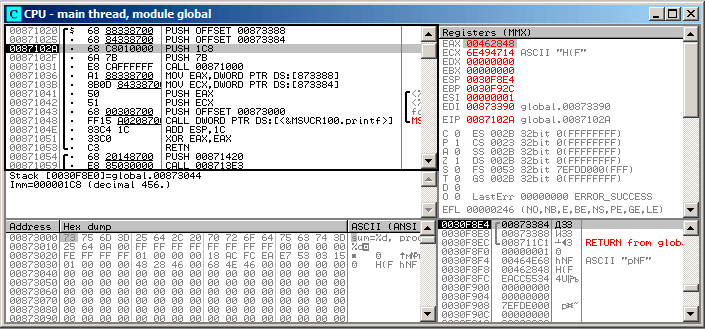
\includegraphics[scale=\FigScale]{patterns/061_pointers/olly_global1.png}
\caption{\olly: \RU{передаются адреса двух глобальных переменных в}
\EN{global variables addresses are passed to} \ttfone}
\label{fig:pointers_olly_global_1}
\end{figure}

\RU{В начале адреса обоих глобальных переменных передаются в}\EN{First, global
variables' addresses are passed to} \ttfone.
\RU{Можно нажать}\EN{We can click} \q{Follow in dump} 
\RU{на элементе стека и в окне слева 
увидим место в сегменте данных, выделенное для двух переменных.}
\EN{on the stack element, and we can see the place in the data segment allocated 
for the two variables.}
\RU{Эти переменные обнулены, потому что по стандарту неинициализированные данные (\ac{BSS}) 
обнуляются перед началом исполнения: \cite[6.7.8p10]{C99TC3}.}

\clearpage
\EN{These variables are zeroed, because non-initialized data (from \ac{BSS}) is cleared before
the execution begins: \cite[6.7.8p10]{C99TC3}.}
\RU{И они находятся в сегменте данных, о чем можно удостовериться, нажав}
\EN{They reside in the data segment, we can verify this by pressing} Alt-M \RU{и увидев карту
памяти}\EN{and reviewing the memory map}:

\begin{figure}[H]
\centering
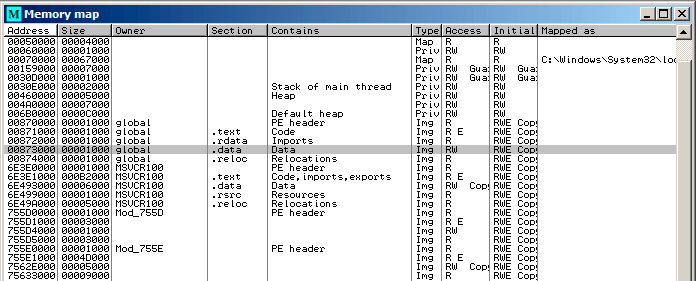
\includegraphics[scale=\FigScale]{patterns/061_pointers/olly_global5.png}
\caption{\olly: \RU{карта памяти}\EN{memory map}}
\label{fig:pointers_olly_global_5}
\end{figure}

\clearpage
\RU{Трассируем}\EN{Let's trace} (F7) \RU{до начала исполнения}\EN{to the start of} \ttfone: 

\begin{figure}[H]
\centering
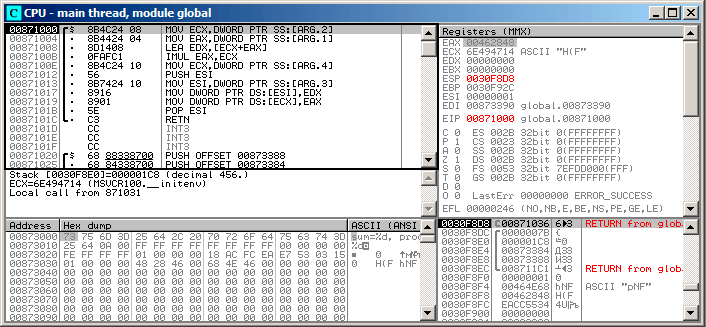
\includegraphics[scale=\FigScale]{patterns/061_pointers/olly_global2.png}
\caption{\olly: \RU{начало работы \ttfone}\EN{\ttfone starts}}
\label{fig:pointers_olly_global_2}
\end{figure}

\RU{В стеке видны значения}\EN{Two values are visible in the stack} 456 (\TT{0x1C8}) \AndENRU 
123 (\TT{0x7B}), \RU{а также адреса двух глобальных переменных}\EN{and also the addresses of the two global variables}.

\clearpage
\RU{Трассируем до конца}\EN{Let's trace until the end of} \ttfone.
\RU{Мы видим в окне слева, как результаты вычисления появились в глобальных переменных}%
\EN{In the left bottom window we see how the results of the calculation appear in the global variables}: 

\begin{figure}[H]
\centering
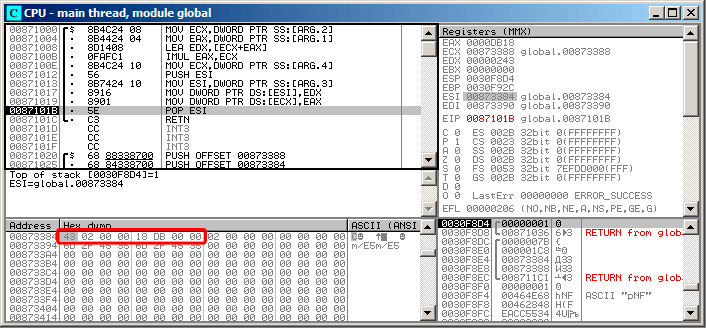
\includegraphics[scale=\FigScale]{patterns/061_pointers/olly_global3.png}
\caption{\olly: \ttfone \RU{заканчивает работу}\EN{execution completed}}
\label{fig:pointers_olly_global_3}
\end{figure}

\clearpage
\RU{Теперь из глобальных переменных значения загружаются в регистры для передачи в}
\EN{Now the global variables' values are loaded into registers ready for passing to} \printf \EN{(via the stack)}:

\begin{figure}[H]
\centering
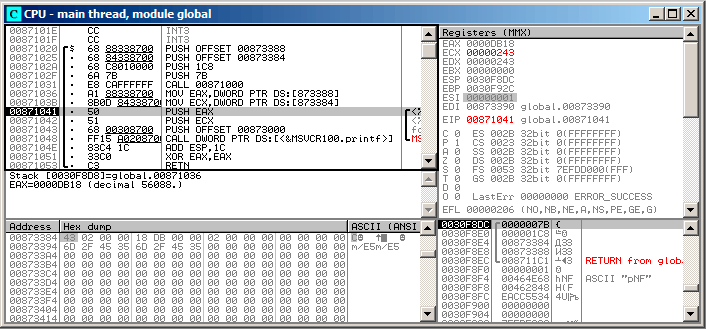
\includegraphics[scale=\FigScale]{patterns/061_pointers/olly_global4.png}
\caption{\olly: \RU{адреса глобальных переменных передаются в}
\EN{global variables' addresses are passed into} \printf}
\label{fig:pointers_olly_global_4}
\end{figure}

\section{\RU{Пример с локальными переменными}\EN{Local variables example}}

\RU{Немного переделаем пример}\EN{Let's rework our example slightly}:

\lstinputlisting[caption=\RU{теперь переменные локальные}
\EN{now the \TT{sum} and \TT{product} variables are local}]{patterns/061_pointers/local.c.\LANG}

\RU{Код функции }\ttfone \RU{не изменится}\EN{code will not change}.
\RU{Изменится только \main}\EN{Only the code of \main will do}:

\lstinputlisting[caption=\Optimizing MSVC 2010 (/Ob0)]{patterns/061_pointers/local.asm}

\newcommand{\PtrsAddresses}{\TT{0x2EF854} \AndENRU \TT{0x2EF858}\xspace}

\clearpage
\RU{Снова посмотрим в}\EN{Let's look again with} \olly.
\RU{Адреса локальных переменных в стеке это}\EN{The addresses of the local variables in the stack are} \PtrsAddresses.
\RU{Видно, как они заталкиваются в стек}\EN{We see how these are pushed into the stack}: 

\begin{figure}[H]
\centering
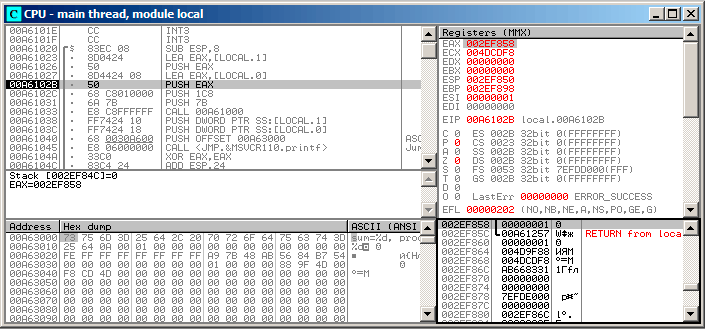
\includegraphics[scale=\FigScale]{patterns/061_pointers/olly_stk1.png}
\caption{\olly: \RU{адреса локальных переменных заталкиваются в стек}\EN{local variables' addresses are
pushed into the stack}}
\label{fig:pointers_olly_stk_1}
\end{figure}

\clearpage
\RU{Начало работы \ttfone}\EN{\ttfone starts}.
\RU{В стеке по адресам}\EN{So far there is only random garbage in the stack at} \PtrsAddresses \RU{пока находится случайный мусор}:

\begin{figure}[H]
\centering
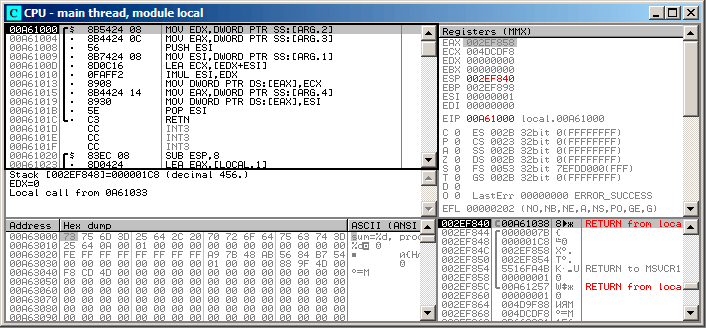
\includegraphics[scale=\FigScale]{patterns/061_pointers/olly_stk2.png}
\caption{\olly: \ttfone \RU{начинает работу}\EN{starting}}
\label{fig:pointers_olly_stk_2}
\end{figure}

\clearpage
\RU{Конец работы \ttfone}\EN{\ttfone completes}:

\begin{figure}[H]
\centering
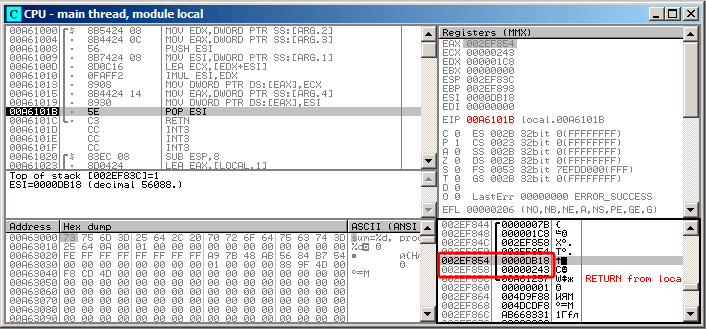
\includegraphics[scale=\FigScale]{patterns/061_pointers/olly_stk3.png}
\caption{\olly: \ttfone \RU{заканчивает работу}\EN{completes execution}}
\label{fig:pointers_olly_stk_3}
\end{figure}

\RU{В стеке по адресам \PtrsAddresses теперь находятся значения \TT{0xDB18} \AndENRU \TT{0x243}, 
это результаты работы \ttfone.}
\EN{We now find \TT{0xDB18} \AndENRU \TT{0x243} at addresses \PtrsAddresses. These values are
the \ttfone results.}

\section{\Conclusion{}}

\RU{\ttfone может одинаково хорошо возвращать результаты работы в любые места памяти.} 
\EN{\ttfone could return pointers to any place in memory, located anywhere.}
\RU{В этом суть и удобство указателей.}
\EN{This is in essence the usefulness of the pointers.}

\RU{Кстати,}\EN{By the way, \Cpp} \IT{references} \RU{в \Cpp работают точно так же}\EN{work exactly the
same way}. \RU{Читайте больше об этом}\EN{Read more about them}: (\myref{cpp_references}).

\fi
\chapter{\RU{Оператор GOTO}\EN{GOTO operator}}

\RU{Оператор GOTO считается анти-паттерном}\EN{The GOTO operator is generally considered as anti-pattern.} 
\cite{Dijkstra:1968:LEG:362929.362947}, 
\RU{но тем не менее, его можно использовать в разумных пределах}
\EN{Nevertheless, it can be used reasonably} \cite{Knuth:1974:SPG:356635.356640}, \cite[1.3.2]{CBook}.

\RU{Вот простейший пример}\EN{Here is a very simple example}:

\lstinputlisting{patterns/065_GOTO/goto.c}

\RU{Вот что мы получаем в}\EN{Here is what we have got in} MSVC 2012:

\lstinputlisting[caption=MSVC 2012]{patterns/065_GOTO/MSVC_goto.asm}

\RU{Выражение \IT{goto} заменяется инструкцией \JMP, которая работает точно также:
безусловный переход в другое место.}
\EN{The \IT{goto} statement has been simply replaced by a \JMP instruction, which has the same
effect: unconditional jump to another place.}

\RU{Вызов второго \printf может исполнится только при помощи человеческого вмешательства,
используя отладчик или модифицирование кода.}
\EN{The second \printf could be executed only with human intervention, 
by using a debugger or by patching the code.}
\PTBRph{}\ESph{}\PLph{}\\
\\
\ifdefined\IncludeHiew
\clearpage
\RU{Это также может быть простым упражнением на модификацию кода.}
\EN{This could also be useful as a simple patching exercise.}
\RU{Откроем исполняемый файл в}\EN{Let's open the resulting executable in} Hiew:

\begin{figure}[H]
\centering
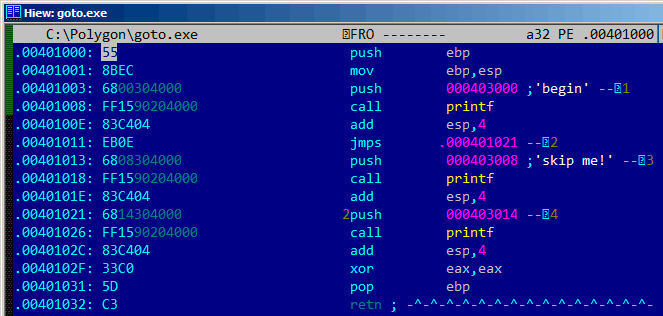
\includegraphics[scale=\FigScale]{patterns/065_GOTO/hiew1.png}
\caption{Hiew}
\label{fig:goto_hiew1}
\end{figure}

\clearpage
\RU{Поместите курсор по адресу}\EN{Place the cursor to address} \JMP (\TT{0x410}), 
\RU{нажмите}\EN{press} F3 (\RU{редактирование}\EN{edit}), \RU{нажмите два нуля, так что
опкод становится}\EN{press zero twice, so the opcode becomes} \TT{EB 00}:

\begin{figure}[H]
\centering
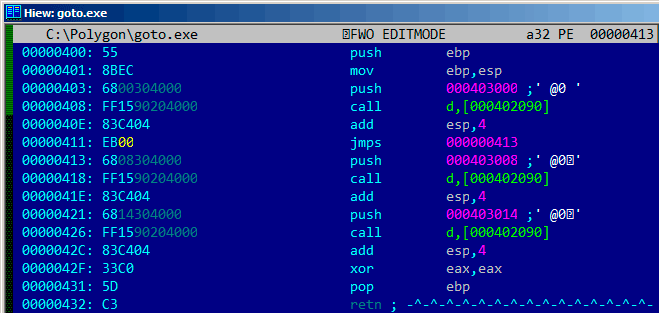
\includegraphics[scale=\FigScale]{patterns/065_GOTO/hiew2.png}
\caption{Hiew}
\label{fig:goto_hiew2}
\end{figure}

\RU{Второй байт опкода \JMP это относительное смещение от перехода. 0 означает место
прямо после текущей инструкции.}
\EN{The second byte of the \JMP opcode denotes the relative offset for the jump, 0 means the point
right after the current instruction.}
\RU{Теперь \JMP не будет пропускать следующий вызов \printf.}
\EN{So now \JMP not skipping the second \printf call.}

\RU{Нажмите F9 (запись) и выйдите.}
\EN{Press F9 (save) and exit.}
\RU{Теперь мы запускаем исполняемый файл и видим это}\EN{Now if we run the executable we should see 
this}:

\begin{figure}[H]
\centering
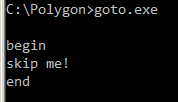
\includegraphics[scale=\NormalScale]{patterns/065_GOTO/result.png}
\caption{\RU{Результат}\EN{Patched executable output}}
\label{fig:goto_result}
\end{figure}

\RU{Подобного же эффекта можно достичь, если заменить инструкцию \JMP на две инструкции \NOP.}
\EN{The same result could be achieved by replacing the \JMP instruction with 2 \NOP instructions.}
\RU{\NOP имеет опкод \TT{0x90} и длину в 1 байт, так что нужно 2 инструкции для замены.}
\EN{\NOP has an opcode of \TT{0x90} and length of 1 byte, so we need 2 instructions as \JMP replacement (which is 2 bytes in size).}
\fi

\section{\RU{Мертвый код}\EN{Dead code}}

\RU{Вызов второго \printf также называется \q{мертвым кодом} (\q{dead code}) 
в терминах компиляторов.}
\EN{The second \printf call is also called \q{dead code} in compiler terms.}
\RU{Это значит, что он никогда не будет исполнен.}
\EN{This means that the code will never be executed.}
\EN{So when you compile this example with optimizations, the compiler removes \q{dead code}, leaving
no trace of it:}
\RU{Так что если вы компилируете этот пример с оптимизацией, компилятор удаляет \q{мертвый
код} не оставляя следа:}

\lstinputlisting[caption=\Optimizing MSVC 2012]{patterns/065_GOTO/MSVC_goto_Ox.asm}

\RU{Впрочем, строку}\EN{However, the compiler forgot to remove the} \q{skip me!} \RU{компилятор 
убрать забыл}\EN{string}.

%Note: cl "/Ox" option for maximum optimisation does get rid of "skip me" string as well

\ifdefined\IncludeExercises
\section{\Exercise}

% TODO debugger example can fit here
\RU{Попробуйте добиться того же самого в вашем любимом компиляторе и отладчике.}
\EN{Try to achieve the same result using your favorite compiler and debugger.}
\fi

\chapter{\RU{Условные переходы}\EN{Conditional jumps}}
\label{sec:Jcc}
\index{\CLanguageElements!if}

% sections
\input{patterns/07_jcc/simple/main}
\input{patterns/07_jcc/abs/main}
\input{patterns/07_jcc/cond_operator/main}
\input{patterns/07_jcc/minmax/main}

\section{\Conclusion{}}

\subsection{x86}

\RU{Примерный скелет условных переходов}\EN{Here's the rough skeleton of a conditional jump}:

\lstinputlisting[caption=x86]{patterns/07_jcc/skel1.lst.\LANG}

\ifdefined\IncludeARM

\subsection{ARM}

\lstinputlisting[caption=ARM]{patterns/07_jcc/skel2.lst.\LANG}
\fi

\ifdefined\IncludeMIPS

\subsection{MIPS}

\begin{lstlisting}[caption=\RU{Проверка на ноль}\EN{Check for zero}]
BEQZ REG, label
...
\end{lstlisting}

\begin{lstlisting}[caption=\RU{Меньше ли нуля?}\EN{Check for less than zero:}]
BLTZ REG, label
...
\end{lstlisting}

\begin{lstlisting}[caption=\RU{Проверка на равенство}\EN{Check for equal values}]
BEQ REG1, REG2, label
...
\end{lstlisting}

\begin{lstlisting}[caption=\RU{Проверка на неравенство}\EN{Check for non-equal values}]
BNE REG1, REG2, label
...
\end{lstlisting}

\begin{lstlisting}[caption=\RU{Проверка на меньше, больше (знаковое)}\EN{Check for less than, greater than (signed)}]
SLT REG1, REG2, REG3
BEQ REG1, label
...
\end{lstlisting}

\begin{lstlisting}[caption=\RU{Проверка на меньше, больше (беззнаковое)}\EN{Check for less than, greater than (unsigned)}]
SLTU REG1, REG2, REG3
BEQ REG1, label
...
\end{lstlisting}
\fi

\subsection{\RU{Без инструкций перехода}\EN{Branchless}}

\index{ARM!\Instructions!MOVcc}
\index{x86!\Instructions!CMOVcc}
\index{ARM!\Instructions!CSEL}
\EN{If the body of a condition statement is very short, the conditional move instruction can be used: 
MOVcc in ARM (in ARM mode), CSEL in ARM64, CMOVcc in x86.}
\RU{Если тело условного выражения очень короткое, может быть
использована инструкция условного копирования: MOVcc в ARM (в режиме ARM), CSEL в ARM64, CMOVcc в x86.}

\ifdefined\IncludeARM
\subsubsection{ARM}

\RU{В режиме ARM можно использовать условные суффиксы для некоторых инструкций:}
\EN{It's possible to use conditional suffixes in ARM mode for some instructions:}

\lstinputlisting[caption=ARM (\ARMMode)]{patterns/07_jcc/skel4.lst.\LANG}

\RU{Нет никаких ограничений на количество инструкций с условными суффиксами до тех пор,
пока флаги CPU не были модифицированы одной из таких инструкций.}
\EN{Of course, there is no limit for the number of instructions with conditional code suffixes, 
as long as the CPU flags are not modified by any of them.}
% FIXME: list of such instructions or \myref{} to it

\index{ARM!\Instructions!IT}
\RU{В режиме Thumb есть инструкция IT, позволяющая дополнить следующие 4 инструкции суффиксами, задающими
условие.}
\EN{Thumb mode has the IT instruction, allowing to add conditional suffixes to the next four instructions.}
\RU{Читайте больше об этом}\EN{Read more about it}: \myref{ARM_Thumb_IT}.

\lstinputlisting[caption=ARM (\ThumbMode)]{patterns/07_jcc/skel3.lst.\LANG}
\fi

\ifdefined\IncludeExercises
\section{\Exercise}

(ARM64) \RU{Попробуйте переписать код в}\EN{Try rewriting the code in} \lstref{cond_ARM64} 
\RU{убрав все инструкции условного перехода, и используйте инструкцию \TT{CSEL}}\EN{by removing all 
conditional jump instructions and using the \TT{CSEL} instruction}.
\fi


\chapter{\SwitchCaseDefaultSectionName}
\index{\CLanguageElements!switch}

% sections
\input{patterns/08_switch/1_few/main}
\input{patterns/08_switch/2_lot/main}
% TODO What's the difference between 3 and 4? Seems to be the same...
% it is fallthrough from 3 to 4 :) --DY
\input{patterns/08_switch/3_several_cases/main}
\input{patterns/08_switch/4_fallthrough/main}

\ifdefined\IncludeExercises
\section{\Exercises}

\subsection{\Exercise \#1}
\label{exercise_switch_1}

\RU{Вполне возможно переделать пример на Си в листинге \myref{switch_lot_c} так, чтобы при компиляции
получалось даже ещё меньше кода, но работать всё будет точно так же.}
\EN{It's possible to rework the C example in \myref{switch_lot_c} in such way that the compiler
can produce even smaller code, but will work just the same.}
\RU{Попробуйте этого добиться}\EN{Try to achieve it}.

\RU{Подсказка}\EN{Hint}: \myref{exercise_solutions_switch_1}.
\fi

\chapter{\Loops}
\label{sec:loops}

% sections
\input{patterns/09_loops/simple/main}
\input{patterns/09_loops/memcpy/main}
\input{patterns/09_loops/conclusion}
\ifdefined\IncludeExercises
\input{patterns/09_loops/exercises}
\fi

\chapter{\SimpleStringsProcessings}
\index{\CStandardLibrary!strlen()}
\index{\CLanguageElements!while}

% sections
\input{patterns/10_strings/1_strlen/main}
\ifdefined\IncludeExercises
\input{patterns/10_strings/exercises}
\fi

\chapter{\ArithOptimizations}

\RU{В целях оптимизации одна инструкция может быть заменена другой, или даже группой инструкций.}
\EN{In the pursuit of optimization, one instruction may be replaced by another, 
or even with a group of instructions.} \RU{Например}\EN{For example}, \ADD \AndENRU \SUB \RU{могут заменять друг друга}\EN{can replace each other}:
\LineENRU 18 \InENRU \lstref{neg_array_c}.

\ifx\LITE\undefined
\RU{Более того, не всегда замена тривиальна. Инструкция \LEA, несмотря на оригинальное назначение, нередко применяется для простых арифметических действий:}
\EN{For example, the \LEA instruction is often used for simple arithmetic calculations:}  \myref{sec:LEA}.

\fi

% sections
\input{patterns/11_arith_optimizations/mult}
\input{patterns/11_arith_optimizations/div}
\ifdefined\IncludeExercises
\input{patterns/11_arith_optimizations/exercises}
\fi

\ifx\LITE\undefined
\chapter{\FPUChapterName}
\label{sec:FPU}

\newcommand{\FNURLSTACK}{\footnote{\href{http://go.yurichev.com/17123}{wikipedia.org/wiki/Stack\_machine}}}
\newcommand{\FNURLFORTH}{\footnote{\href{http://go.yurichev.com/17124}{wikipedia.org/wiki/Forth\_(programming\_language)}}}
\newcommand{\FNURLIEEE}{\footnote{\href{http://go.yurichev.com/17125}{wikipedia.org/wiki/IEEE\_floating\_point}}}
\newcommand{\FNURLSP}{\footnote{\href{http://go.yurichev.com/17126}{wikipedia.org/wiki/Single-precision\_floating-point\_format}}}
\newcommand{\FNURLDP}{\footnote{\href{http://go.yurichev.com/17127}{wikipedia.org/wiki/Double-precision\_floating-point\_format}}}
\newcommand{\FNURLEP}{\footnote{\href{http://go.yurichev.com/17128}{wikipedia.org/wiki/Extended\_precision}}}

\RU{\ac{FPU}\EMDASH блок в процессоре работающий с числами с плавающей запятой.}
\EN{The \ac{FPU} is a device within the main \ac{CPU}, specially designed to deal with floating point numbers.}
\RU{Раньше он назывался \q{сопроцессором} и он стоит немного в стороне от \ac{CPU}.}
\EN{It was called \q{coprocessor} in the past and it stays somewhat aside of the main \ac{CPU}.}

\section{IEEE 754}

\RU{Число с плавающей точкой в формате IEEE 754 состоит из \IT{знака}, \IT{мантиссы}\footnote{\IT{significand} или \IT{fraction} 
в англоязычной литературе} и \IT{экспоненты}.}
\EN{A number in the IEEE 754 format consists of a \IT{sign}, a \IT{significand} (also called \IT{fraction}) and an \IT{exponent}.}

\section{x86}

\RU{Перед изучением \ac{FPU} в x86 полезно ознакомиться с тем как работают стековые машины\FNURLSTACK 
или ознакомиться с основами языка Forth\FNURLFORTH.}
\EN{It is worth looking into stack machines\FNURLSTACK or learning the basics of the Forth language\FNURLFORTH,
before studying the \ac{FPU} in x86.}

\index{Intel!80486}
\index{Intel!FPU}
\RU{Интересен факт, что в свое время (до 80486) сопроцессор был отдельным чипом на материнской плате, 
и вследствие его высокой цены, он не всегда присутствовал. Его можно было докупить и установить отдельно}%
\EN{It is interesting to know that in the past (before the 80486 CPU) the coprocessor was a separate chip 
and it was not always pre-installed on the motherboard. It was possible to buy it separately and install it}%
\footnote{\RU{Например, Джон Кармак использовал в своей игре Doom числа с фиксированной запятой 
(\href{http://go.yurichev.com/17357}{ru.wikipedia.org/wiki/Число\_с\_фиксированной\_запятой}), хранящиеся
в обычных 32-битных \ac{GPR} (16 бит на целую часть и 16 на дробную),
чтобы Doom работал на 32-битных компьютерах без FPU, т.е. 80386 и 80486 SX.}
\EN{For example, John Carmack used fixed-point arithmetic 
(\href{http://go.yurichev.com/17356}{wikipedia.org/wiki/Fixed-point\_arithmetic}) values in his Doom video game, stored in 
32-bit \ac{GPR} registers (16 bit for integral part and another 16 bit for fractional part), so Doom
could work on 32-bit computers without FPU, i.e., 80386 and 80486 SX.}}.
\RU{Начиная с 80486 DX в состав процессора всегда входит FPU.}
\EN{Starting with the 80486 DX CPU, the \ac{FPU} is integrated in the \ac{CPU}.}

\index{x86!\Instructions!FWAIT}
\RU{Этот факт может напоминать такой рудимент как наличие инструкции \TT{FWAIT}, 
которая заставляет
\ac{CPU} ожидать, пока \ac{FPU} закончит работу}\EN{The \TT{FWAIT} instruction reminds us of that fact---it
switches the \ac{CPU} to a waiting state, so it can wait until the \ac{FPU} is done with its work}.
\RU{Другой рудимент это тот факт, что опкоды \ac{FPU}-инструкций начинаются с т.н. \q{escape}-опкодов 
(\TT{D8..DF}) как опкоды, передающиеся в отдельный сопроцессор.}
\EN{Another rudiment is the fact that the \ac{FPU} instruction 
opcodes start with the so called \q{escape}-opcodes (\TT{D8..DF}), i.e., 
opcodes passed to a separate coprocessor.}

\index{IEEE 754}
\label{FPU_is_stack}
\RU{FPU имеет стек из восьми 80-битных регистров:}
\EN{The FPU has a stack capable to holding 8 80-bit registers, and each register can hold a number 
in the IEEE 754\FNURLIEEE format.}
\RU{\ST{0}..\ST{7}. Для краткости, IDA и \olly отображают \ST{0} как \TT{ST},
что в некоторых учебниках и документациях означает \q{Stack Top} (\q{вершина стека}).}
\RU{Каждый регистр может содержать число в формате IEEE 754\FNURLIEEE.}
\EN{They are \ST{0}..\ST{7}. For brevity, IDA and \olly show \ST{0} as \TT{ST}, 
which is represented in some textbooks and manuals as \q{Stack Top}.}

\section{ARM, MIPS, x86/x64 SIMD}

\RU{В ARM и MIPS FPU это не стек, а просто набор регистров.}
\EN{In ARM and MIPS the FPU is not a stack, but a set of registers.}
\RU{Такая же идеология применяется в расширениях SIMD в процессорах x86/x64.}
\EN{The same ideology is used in the SIMD extensions of x86/x64 CPUs.}

\section{\CCpp}

\index{float}
\index{double}
\RU{В стандартных \CCpp имеются два типа для работы с числами с плавающей запятой: 
\Tfloat (\IT{число одинарной точности}\FNURLSP, 32 бита)
\footnote{Формат представления чисел с плавающей точкой одинарной точности затрагивается в разделе 
\IT{\WorkingWithFloatAsWithStructSubSubSectionName}~(\myref{sec:floatasstruct}).}
и \Tdouble (\IT{число двойной точности}\FNURLDP, 64 бита).}
\EN{The standard \CCpp languages offer at least two floating number types, \Tfloat (\IT{single-precision}\FNURLSP, 32 bits)
\footnote{the single precision floating point number format is also addressed in 
the \IT{\WorkingWithFloatAsWithStructSubSubSectionName}~(\myref{sec:floatasstruct}) section}
and \Tdouble (\IT{double-precision}\FNURLDP, 64 bits).}

\index{long double}
\RU{GCC также поддерживает тип \IT{long double} (\IT{extended precision}\FNURLEP, 80 бит), но MSVC~--- нет.}
\EN{GCC also supports the \IT{long double} type (\IT{extended precision}\FNURLEP, 80 bit), which MSVC doesn't.}

\RU{Несмотря на то, что \Tfloat занимает столько же места, сколько и \Tint на 32-битной архитектуре, 
представление чисел, разумеется, совершенно другое.}
\EN{The \Tfloat type requires the same number of bits as the \Tint type in 32-bit environments, 
but the number representation is completely different.}

\input{patterns/12_FPU/1_simple/main}
\input{patterns/12_FPU/2_passing_floats/main}
\input{patterns/12_FPU/3_comparison/main}

\section{\RU{Стек, калькуляторы и обратная польская запись}\EN{Stack, calculators and reverse Polish notation}}

\index{\RU{Обратная польская запись}\EN{Reverse Polish notation}}
\RU{Теперь понятно, почему некоторые старые калькуляторы использовали обратную польскую запись%
\footnote{\href{http://go.yurichev.com/17355}{ru.wikipedia.org/wiki/Обратная\_польская\_запись}}.}
\EN{Now we undestand why some old calculators used reverse Polish notation
\footnote{\href{http://go.yurichev.com/17354}{wikipedia.org/wiki/Reverse\_Polish\_notation}}.}
\RU{Например для сложения 12 и 34 нужно было набрать 12, потом 34, потом нажать знак \q{плюс}.}
\EN{For example, for addition of 12 and 34 one has to enter 12, then 34, then press \q{plus} sign.}
\RU{Это потому что старые калькуляторы просто реализовали стековую машину и это было куда проще, 
чем обрабатывать сложные выражения со скобками.}
\EN{It's because old calculators were just stack machine implementations, and this was much simpler
than to handle complex parenthesized expressions.}
\section{x64}

\RU{О том, как происходит работа с числами с плавающей запятой в x86-64, читайте здесь: \myref{floating_SIMD}.}
\EN{On how floating point numbers are processed in x86-64, read more here: \myref{floating_SIMD}.}

% sections
\ifdefined\IncludeExercises
\input{patterns/12_FPU/exercises}
\fi

\fi
\chapter{\Arrays}
\label{arrays}

\RU{Массив это просто набор переменных в памяти, 
обязательно лежащих рядом и обязательно одного типа%
\footnote{\ac{AKA} \q{гомогенный контейнер}}.}
\EN{An array is just a set of variables in memory 
that lie next to each other and that have the same type%
\footnote{\ac{AKA} \q{homogeneous container}}.}

% sections
\input{patterns/13_arrays/1_simple/main}
\input{patterns/13_arrays/2_BO/main}
\ifx\LITE\undefined
\input{patterns/13_arrays/3_BO_protection/main}
\fi
\input{patterns/13_arrays/4_one_more_thing/main}
\input{patterns/13_arrays/45_month_1D/main}
\input{patterns/13_arrays/5_multidimensional/main}
\ifx\LITE\undefined
\input{patterns/13_arrays/55_month_2D/main}
\fi
\input{patterns/13_arrays/conclusion}
\ifdefined\IncludeExercises
\input{patterns/13_arrays/exercises}
\fi

\chapter{\BitfieldsChapter}
\label{sec:bitfields}

\RU{Немало функций задают различные флаги в аргументах при помощи битовых 
полей\footnote{bit fields в англоязычной литературе}.}
\EN{A lot of functions define their input arguments as flags in bit fields.}
\index{\CLanguageElements!C99!bool}
\RU{Наверное, вместо этого можно было бы использовать набор переменных типа \Tbool, но это было бы 
не очень экономно.}
\EN{Of course, they could be substituted by a set of \Tbool-typed variables, but it is not frugally.}

% sections
\input{patterns/14_bitfields/1_check/main}
\input{patterns/14_bitfields/2_set_reset/main}
\input{patterns/14_bitfields/3_shifts/main}
\ifx\LITE\undefined
\input{patterns/14_bitfields/35_set_reset_FPU/main}
\fi
\input{patterns/14_bitfields/4_popcnt/main}
\input{patterns/14_bitfields/conclusion}
\ifdefined\IncludeExercises
\input{patterns/14_bitfields/exercises}
\fi

\chapter[\RU{Линейный конгруэнтный генератор}\EN{Linear congruential generator}]
{\RU{Линейный конгруэнтный генератор как генератор псевдослучайных чисел}\EN{Linear congruential generator as pseudorandom number generator}}
\index{\CStandardLibrary!rand()}
\label{LCG_simple}

\RU{Линейный конгруэнтный генератор, пожалуй, самый простой способ генерировать псевдослучайные числа.}
\EN{The linear congruential generator is probably the simplest possible way to generate random numbers.}
\RU{Он не в почете в наше время\footnote{Вихрь Мерсенна куда лучше}, но он настолько прост
(только одно умножение, одно сложение и одна операция \q{И}),
что мы можем использовать его в качестве примера.}
\EN{It's not in favour in modern times\footnote{Mersenne twister is better}, but it's so simple 
(just one multiplication, one addition and one AND operation), 
we can use it as an example.}

\lstinputlisting{patterns/145_LCG/rand.c.\LANG}

\RU{Здесь две функции: одна используется для инициализации внутреннего состояния, а вторая
вызывается собственно для генерации псевдослучайных чисел.}
\EN{There are two functions: the first one is used to initialize the internal state, and the second one is called
to generate pseudorandom numbers.}

\RU{Мы видим что в алгоритме применяются две константы}\EN{We see that two constants are used in the algorithm}.
\RU{Они взяты из}\EN{They are taken from} \cite{Numerical}.
\RU{Определим их используя выражение \CCpp \TT{\#define}. Это макрос.}
\EN{Let's define them using a \TT{\#define} \CCpp statement. It's a macro.}
\RU{Разница между макросом в \CCpp и константой в том, что все макросы заменяются на значения препроцессором
\CCpp и они не занимают места в памяти как переменные.}
\EN{The difference between a \CCpp macro and a constant is that all macros are replaced 
with their value by \CCpp preprocessor,
and they don't take any memory, unlike variables.}
\RU{А константы, напротив, это переменные только для чтения.}
\EN{In contrast, a constant is a read-only variable.}
\RU{Можно взять указатель (или адрес) переменной-константы, но это невозможно сделать с макросом.}
\EN{It's possible to take a pointer (or address) of a constant variable, but impossible to do so with a macro.}

\RU{Последняя операция \q{И} нужна, потому что согласно стандарту Си \TT{my\_rand()} должна возвращать значение в пределах
0..32767.}
\EN{The last AND operation is needed because by C-standard \TT{my\_rand()} has to return a value in 
the 0..32767 range.}
\RU{Если вы хотите получать 32-битные псевдослучайные значения, просто уберите последнюю операцию \q{И}.}
\EN{If you want to get 32-bit pseudorandom values, just omit the last AND operation.}

\section{x86}

\lstinputlisting[caption=\Optimizing MSVC 2013]{patterns/145_LCG/rand_MSVC_2013_x86_Ox.asm}

\RU{Вот мы это и видим: обе константы встроены в код.}
\EN{Here we see it: both constants are embedded into the code.}
\RU{Память для них не выделяется.}\EN{There is no memory allocated for them.}
\RU{Функция \TT{my\_srand()} просто копирует входное значение во внутреннюю переменную \TT{rand\_state}.}
\EN{The \TT{my\_srand()} function just copies its input value into the internal \TT{rand\_state} variable.}

\RU{\TT{my\_rand()} берет её, вычисляет следующее состояние \TT{rand\_state}, 
обрезает его и оставляет в регистре EAX.}
\EN{\TT{my\_rand()} takes it, calculates the next \TT{rand\_state}, cuts it and leaves it in the EAX register.}

\RU{Неоптимизированная версия побольше}\EN{The non-optimized version is more verbose}:

\lstinputlisting[caption=\NonOptimizing MSVC 2013]{patterns/145_LCG/rand_MSVC_2013_x86.asm}

\section{x64}

\RU{Версия для x64 почти такая же, и использует 32-битные регистры вместо 64-битных
(потому что мы работаем здесь с переменными типа \Tint).}
\EN{The x64 version is mostly the same and uses 32-bit registers instead of 64-bit ones 
(because we are working with \Tint values here).}
\RU{Но функция \TT{my\_srand()} берет входной аргумент из регистра \ECX, а не из стека:}
\EN{But \TT{my\_srand()} takes its input argument from the \ECX register rather than from stack:}

\lstinputlisting[caption=\Optimizing MSVC 2013 x64]{patterns/145_LCG/rand_MSVC_2013_x64_Ox.asm.\LANG}

\ifdefined\IncludeGCC
\RU{GCC делает почти такой же код}\EN{GCC compiler generates mostly the same code}.
\fi

\ifdefined\IncludeARM
\section{32-bit ARM}

\lstinputlisting[caption=\OptimizingKeilVI (\ARMMode)]{patterns/145_LCG/rand.s_Keil_ARM_O3.s.\LANG}

\RU{В ARM инструкцию невозможно встроить 32-битную константу, так что Keil-у приходится размещать
их отдельно и дополнительно загружать.}
\EN{It's not possible to embed 32-bit constants into ARM instructions, so Keil has to place them externally
and load them additionally.}

\RU{Вот еще что интересно: константу 0x7FFF также нельзя встроить.}
\EN{One interesting thing is that it's not possible to embed the 0x7FFF constant as well.}
\RU{Поэтому Keil сдвигает \TT{rand\_state} влево на 17 бит и затем сдвигает вправо на 17 бит.}
\EN{So what Keil does is shifting \TT{rand\_state} left by 17 bits and then shifting it right by 17 bits.}
\RU{Это аналогично \CCpp{}-выражению $(rand\_state \ll 17) \gg 17$.}
\EN{This is analogous to the $(rand\_state \ll 17) \gg 17$ statement in \CCpp.}
\RU{Выглядит как бессмысленная операция, но тем не менее, что она делает это очищает старшие 17 бит, оставляя
младшие 15 бит нетронутыми, и это наша цель, в конце концов.}
\EN{It seems to be useless operation, but
what it does is clearing the high 17 bits, leaving the low 15 bits intact, and that's our goal after all.}
\ESph{}\PTBRph{}\PLph{}\\
\\
\Optimizing Keil \RU{для режима Thumb делает почти такой же код}\EN{for Thumb mode generates mostly the same code}.
\fi

\ifdefined\IncludeMIPS
\input{patterns/145_LCG/MIPS}
\fi

\ifx\LITE\undefined
\section{\RU{Версия этого примера для многопоточной среды}\EN{Thread-safe version of the example}}

\RU{Версия примера для многопоточной среды будет рассмотрена позже}%
\EN{The thread-safe version of the example is to be demonstrated later}: \myref{LCG_TLS}.
\fi

\chapter{\StructuresChapterName}

\RU{В принципе, структура в \CCpp это, с некоторыми допущениями, просто всегда лежащий рядом, 
и в той же последовательности, набор переменных, не обязательно одного типа
\footnote{\ac{AKA} \q{гетерогенный контейнер}}.}
\EN{A \CCpp structure, with some assumptions, is just a set of variables, always stored
in memory together, not necessary of the same type
\footnote{\ac{AKA} \q{heterogeneous container}}.}

% sections
\input{patterns/15_structs/1_systemtime/main.tex}
\input{patterns/15_structs/2_using_malloc/main.tex}
\ifx\LITE\undefined
\input{patterns/15_structs/3_tm_linux/main.tex}
\fi
\input{patterns/15_structs/4_packing/main.tex}
\input{patterns/15_structs/5_nested/main.tex}
\input{patterns/15_structs/6_bitfields/main.tex}
\ifdefined\IncludeExercises
\input{patterns/15_structs/exercises}
\fi

\ifx\LITE\undefined
\chapter{\RU{Объединения (union)}\EN{Unions}}

\EN{\CCpp \IT{union} is mostly used for interpreting a variable (or memory block) of one data type as a variable of another data type.}
\RU{\IT{union} в \CCpp используется в основном для интерпертации переменной (или блока памяти) одного типа как переменной другого типа.}

% sections
\input{patterns/17_unions/FPU_PRNG/main}
\input{patterns/17_unions/epsilon/main}

\section{\RU{Быстрое вычисление квадратного корня}\EN{Fast square root calculation}}

\RU{Вот где еще можно на практике применить трактовку типа \Tfloat как целочисленного, это быстрое вычисление квадратного корня.}%
\EN{Another well-known algorithm where \Tfloat is interpreted as integer is fast calculation of square root.}

\begin{lstlisting}[caption=\EN{The source code is taken from Wikipedia}\RU{Исходный код взят из Wikipedia}: \url{http://go.yurichev.com/17364}]
/* Assumes that float is in the IEEE 754 single precision floating point format
 * and that int is 32 bits. */
float sqrt_approx(float z)
{
    int val_int = *(int*)&z; /* Same bits, but as an int */
    /*
     * To justify the following code, prove that
     *
     * ((((val_int / 2^m) - b) / 2) + b) * 2^m = ((val_int - 2^m) / 2) + ((b + 1) / 2) * 2^m)
     *
     * where
     *
     * b = exponent bias
     * m = number of mantissa bits
     *
     * .
     */
 
    val_int -= 1 << 23; /* Subtract 2^m. */
    val_int >>= 1; /* Divide by 2. */
    val_int += 1 << 29; /* Add ((b + 1) / 2) * 2^m. */
 
    return *(float*)&val_int; /* Interpret again as float */
}
\end{lstlisting}

\RU{В качестве упражнения, вы можете попробовать скомпилировать эту функцию и разобраться, как она работает.}
\EN{As an exercise, you can try to compile this function and to understand, how it works.}\ESph{}\PTBRph{}\PLph{}\\
\\
\RU{Имеется также известный алгоритм быстрого вычисления}\EN{There is also well-known algorithm of fast calculation of} $\frac{1}{\sqrt{x}}$.
\index{Quake III Arena}
\RU{Алгоритм стал известным, вероятно потому, что был применен в Quake III Arena.}%
\EN{Algorithm became popular, supposedly, because it was used in Quake III Arena.}

\RU{Описание алгоритма есть в}\EN{Algorithm description is present in} Wikipedia:
\EN{\url{http://go.yurichev.com/17360}}\RU{\url{http://go.yurichev.com/17361}}.


\newcommand{\comp}{\TT{comp()}\xspace}
\chapter{\RU{Указатели на функции}\EN{Pointers to functions}}
\label{sec:pointerstofunctions}

\index{\CLanguageElements!\Pointers}
\RU{Указатель на функцию, в целом, как и любой другой указатель, просто адрес, указывающий на начало функции 
в сегменте кода.}
\EN{A pointer to a function, as any other pointer, is just the address of the function's start in its code segment.}

\index{Callbacks}
\RU{Это часто применяется для вызовов т.н. callback-функций}\EN{They are often used for calling callback functions}
\footnote{\href{http://go.yurichev.com/17071}{wikipedia}}.

\RU{Известные примеры:}\EN{Well-known examples are:}

\begin{itemize}
\item
\qsort\footnote{\href{http://go.yurichev.com/17072}{wikipedia}},
{\TT{atexit()}}\footnote{\url{http://go.yurichev.com/17073}} \RU{из стандартной библиотеки Си}\EN{from the standard C library}; 

\item
\RU{сигналы в *NIX ОС}\EN{*NIX OS signals}\footnote{\href{http://go.yurichev.com/17074}{wikipedia}};

\item
\RU{запуск тредов}\EN{thread starting}: \TT{CreateThread()} (win32), \TT{pthread\_create()} (POSIX);

\item
\RU{множество функций win32, например}\EN{lots of win32 functions, like} \TT{EnumChildWindows()}\footnote{\href{http://go.yurichev.com/17075}{MSDN}}.

\item
\EN{lots of places in the Linux kernel, for example the filesystem driver functions are called via
callbacks}\RU{множество мест в ядре Linux, например, функции драйверов файловой системы вызываются
через callback-и}: 
\url{http://go.yurichev.com/17076}

\item
\EN{The GCC plugin functions are also called via callbacks}\RU{функции плагинов GCC также вызываются
через callback-и}: 
\url{http://go.yurichev.com/17077}

\item
\RU{Один из примеров указателей на функции это таблица в оконном менеджере \q{dwm} для Linux,
описывающая шорт-каты.}
\EN{Another example of function pointers is a table in the \q{dwm} Linux window manager that 
defines shortcuts.}
\RU{Каждый шорт-кат имеет соответствующую функцию, которую нужно вызвать, если эта клавиша нажата:}
\EN{Each shortcut has a corresponding function to call if a specific key is pressed:} \href{http://go.yurichev.com/17078}{GitHub}.
\RU{Как мы видим, с такой таблицей намного легче обходится чем с большим выражением switch().}
\EN{As we can see, such table is easier to handle than a large switch() statement.}
\end{itemize}

\index{\CStandardLibrary!qsort()}
\RU{Итак, функция \qsort это реализация алгоритма \q{быстрой сортировки}. 
Функция может сортировать что угодно, 
любые типы данных, но при условии, что вы имеете функцию сравнения этих двух элементов данных и 
\qsort может вызывать её.}
\EN{So, the \qsort function is an implementation of quicksort in the \CCpp standard library. 
The functions is able to sort anything, any type of data, 
as long as you have a function to compare these two elements 
and \qsort is able to call it.}

\RU{Эта функция сравнения может определяться так:}\EN{The comparison function can be defined as:}

\begin{lstlisting}
int (*compare)(const void *, const void *)
\end{lstlisting}

\RU{Воспользуемся немного модифицированным примером, который был найден}
\EN{Let's use a slightly modified example which was found} \href{http://go.yurichev.com/17079}
{\RU{здесь}\EN{here}}:

\lstinputlisting[numbers=left,label=qsort_c_src]{patterns/18_pointers_to_functions/17_1.c}

\section{MSVC}

\RU{Компилируем в MSVC 2010 (некоторые части убраны для краткости) с опцией \Ox}
\EN{Let's compile it in MSVC 2010 (some parts were omitted for the sake of brevity) with \Ox option}:

\lstinputlisting[caption=\Optimizing MSVC 2010: /GS- /MD]{patterns/18_pointers_to_functions/17_2_msvc_Ox.asm}

\RU{Ничего особо удивительного здесь мы не видим. В качестве четвертого аргумента, 
в \qsort просто передается адрес метки \TT{\_comp}, где собственно и располагается функция \comp,
или, можно сказать, самая первая инструкция этой функции.}
\EN{Nothing surprising so far.
As a fourth argument, the address of label \TT{\_comp} is passed, which is just a place
where \comp is located, or, in other words, the address of the very first instruction of 
that function.}

\RU{Как \qsort вызывает её?}\EN{How does \qsort call it?}

\index{Windows!MSVCR80.DLL}
\RU{Посмотрим в MSVCR80.DLL (эта DLL куда в MSVC вынесены функции из стандартных библиотек Си):}
\EN{Let's take a look at this function, located in MSVCR80.DLL (a MSVC DLL module with C standard library functions):}

\lstinputlisting[caption=MSVCR80.DLL]{patterns/18_pointers_to_functions/17_3_MSVCR.lst}

\TT{comp}\EMDASH{}\RU{это четвертый аргумент функции. 
Здесь просто передается управление по адресу, указанному в \TT{comp}. 
Перед этим подготавливается два аргумента для функции \comp. 
Далее, проверяется результат её выполнения.}
\EN{is the fourth function argument.
Here the control gets passed to the address in the \TT{comp} argument.
Before it, two arguments are prepared for \comp. Its result is checked after its execution.}

\RU{Вот почему использование указателей на функции ~--- это опасно. 
Во-первых, если вызвать \qsort с неправильным указателем на функцию, 
то \qsort, дойдя до этого вызова, может передать управление неизвестно куда, 
процесс упадет, и эту ошибку можно будет найти не сразу.}
\EN{That's why it is dangerous to use pointers to functions.
First of all, if you call \qsort with an incorrect function pointer, \qsort may pass control flow
to an incorrect point, the process may crash and this bug will be hard to find.}

\RU{Во-вторых, типизация callback-функции должна строго соблюдаться, 
вызов не той функции с не теми аргументами не того типа, 
может привести к плачевным результатам, 
хотя падение процесса это и не проблема, проблема ~--- это найти ошибку, ведь компилятор 
на стадии компиляции может вас и не предупредить о потенциальных неприятностях.}
\EN{The second reason is that the callback function types must comply strictly, calling the wrong function
with wrong arguments of wrong types may lead to serious problems, however, the crashing of the process is not a 
problem here~---the problem is how to determine the reason for the crash~---because the compiler may be 
silent about the potential problems while compiling.}

\ifdefined\IncludeOlly
\input{patterns/18_pointers_to_functions/olly.tex}
\fi

\subsection{MSVC + tracer}
\index{tracer}

\RU{Посмотрим, какие пары сравниваются}\EN{Let's also see which pairs are compared}.
\RU{Эти 10 чисел будут сортироваться}\EN{These 10 numbers are being sorted}: 
1892, 45, 200, -98, 4087, 5, -12345, 1087, 88, -100000.

\RU{Найдем адрес первой инструкции \CMP в \comp и это \TT{0x0040100C} и мы ставим точку останова на ней:}%
\EN{We got the address of the first \CMP instruction in \comp, it is \TT{0x0040100C} and we've set a breakpoint on it:}

\begin{lstlisting}
tracer.exe -l:17_1.exe bpx=17_1.exe!0x0040100C
\end{lstlisting}

\RU{Получаем информацию о регистрах на точке останова}%
\EN{Now we get some information about the registers at the breakpoint}:

\begin{lstlisting}
PID=4336|New process 17_1.exe
(0) 17_1.exe!0x40100c
EAX=0x00000764 EBX=0x0051f7c8 ECX=0x00000005 EDX=0x00000000
ESI=0x0051f7d8 EDI=0x0051f7b4 EBP=0x0051f794 ESP=0x0051f67c
EIP=0x0028100c
FLAGS=IF
(0) 17_1.exe!0x40100c
EAX=0x00000005 EBX=0x0051f7c8 ECX=0xfffe7960 EDX=0x00000000
ESI=0x0051f7d8 EDI=0x0051f7b4 EBP=0x0051f794 ESP=0x0051f67c
EIP=0x0028100c
FLAGS=PF ZF IF
(0) 17_1.exe!0x40100c
EAX=0x00000764 EBX=0x0051f7c8 ECX=0x00000005 EDX=0x00000000
ESI=0x0051f7d8 EDI=0x0051f7b4 EBP=0x0051f794 ESP=0x0051f67c
EIP=0x0028100c
FLAGS=CF PF ZF IF
...
\end{lstlisting}

\RU{Отфильтруем \TT{EAX} и \TT{ECX} и получим:}%
\EN{Let's filter out \TT{EAX} and \TT{ECX} and we got:}

\begin{lstlisting}
EAX=0x00000764 ECX=0x00000005
EAX=0x00000005 ECX=0xfffe7960
EAX=0x00000764 ECX=0x00000005
EAX=0x0000002d ECX=0x00000005
EAX=0x00000058 ECX=0x00000005
EAX=0x0000043f ECX=0x00000005
EAX=0xffffcfc7 ECX=0x00000005
EAX=0x000000c8 ECX=0x00000005
EAX=0xffffff9e ECX=0x00000005
EAX=0x00000ff7 ECX=0x00000005
EAX=0x00000ff7 ECX=0x00000005
EAX=0xffffff9e ECX=0x00000005
EAX=0xffffff9e ECX=0x00000005
EAX=0xffffcfc7 ECX=0xfffe7960
EAX=0x00000005 ECX=0xffffcfc7
EAX=0xffffff9e ECX=0x00000005
EAX=0xffffcfc7 ECX=0xfffe7960
EAX=0xffffff9e ECX=0xffffcfc7
EAX=0xffffcfc7 ECX=0xfffe7960
EAX=0x000000c8 ECX=0x00000ff7
EAX=0x0000002d ECX=0x00000ff7
EAX=0x0000043f ECX=0x00000ff7
EAX=0x00000058 ECX=0x00000ff7
EAX=0x00000764 ECX=0x00000ff7
EAX=0x000000c8 ECX=0x00000764
EAX=0x0000002d ECX=0x00000764
EAX=0x0000043f ECX=0x00000764
EAX=0x00000058 ECX=0x00000764
EAX=0x000000c8 ECX=0x00000058
EAX=0x0000002d ECX=0x000000c8
EAX=0x0000043f ECX=0x000000c8
EAX=0x000000c8 ECX=0x00000058
EAX=0x0000002d ECX=0x000000c8
EAX=0x0000002d ECX=0x00000058
\end{lstlisting}

\RU{Это}\EN{That's} 34 \RU{пары}\EN{pairs}.
\RU{Следовательно, алгоритму быстрой сортировки нужно 34 операции сравнения для сортировки этих
10-и чисел}\EN{Therefore, the quick sort algorithm needs 34 comparison operations to sort these 10 numbers}.

\clearpage
\subsection{MSVC + tracer (code coverage)}
\index{tracer}

\RU{Но можно также и воспользоваться возможностью tracer накапливать все возможные состояния регистров
и показать их в \IDA}\EN{We can also use the tracer's feature to collect all possible register values
and show them in \IDA}.

\RU{Трассируем все инструкции в функции \comp}\EN{Let's trace all instructions in \comp}:

\begin{lstlisting}
tracer.exe -l:17_1.exe bpf=17_1.exe!0x00401000,trace:cc
\end{lstlisting}

\RU{Получем .idc-скрипт для загрузки в \IDA и загружаем его}
\EN{We get an .idc-script for loading into \IDA and load it}:

\begin{figure}[H]
\centering
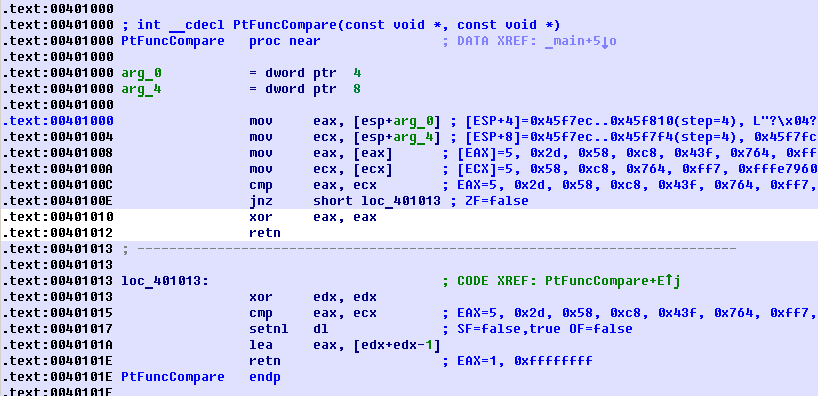
\includegraphics[scale=\FigScale]{patterns/18_pointers_to_functions/tracer_cc.png}
\caption{tracer \AndENRU IDA. N.B.: 
\RU{некоторые значения обрезаны справа}\EN{some values are cut at right}}
\label{fig:qsort_tracer_cc}
\end{figure}

\RU{Имя этой функции (PtFuncCompare) дала \IDA}\EN{\IDA gave the function a name (PtFuncCompare)}
\EMDASH{}\RU{видимо, потому что видит что указатель на эту функцию передается в \qsort}
\EN{because \IDA sees that the pointer to this function is passed to \qsort}.

\RU{Мы видим, что указатели $a$ и $b$ указывают на разные места внутри массива, 
но шаг между указателями --- 4, что логично, ведь в массиве хранятся 32-битные значения}
\EN{We see that the $a$ and $b$ pointers are pointing to various places in the array, but the step between
them is 4, as 32-bit values are stored in the array}.

\RU{Видно, что инструкции по адресам}\EN{We see that the instructions at} \TT{0x401010} \AndENRU 
\TT{0x401012} \RU{никогда не исполнялись}\EN{were never executed} 
(\RU{они и остались белыми}\EN{so they left as white}): 
\RU{действительно, функция}\EN{indeed,} \comp \RU{никогда не возвращала 0,
потому что в массиве нет одинаковых элементов}\EN{has never returned 0, because there no equal elements in the array}.

\ifdefined\IncludeGCC
\section{GCC}

\RU{Не слишком большая разница}\EN{Not a big difference}:

\begin{lstlisting}[caption=GCC]
                lea     eax, [esp+40h+var_28]
                mov     [esp+40h+var_40], eax
                mov     [esp+40h+var_28], 764h
                mov     [esp+40h+var_24], 2Dh
                mov     [esp+40h+var_20], 0C8h
                mov     [esp+40h+var_1C], 0FFFFFF9Eh
                mov     [esp+40h+var_18], 0FF7h
                mov     [esp+40h+var_14], 5
                mov     [esp+40h+var_10], 0FFFFCFC7h
                mov     [esp+40h+var_C], 43Fh
                mov     [esp+40h+var_8], 58h
                mov     [esp+40h+var_4], 0FFFE7960h
                mov     [esp+40h+var_34], offset comp
                mov     [esp+40h+var_38], 4
                mov     [esp+40h+var_3C], 0Ah
                call    _qsort
\end{lstlisting}

\RU{Функция \comp}\EN{\comp function}:

\begin{lstlisting}
                public comp
comp            proc near

arg_0           = dword ptr  8
arg_4           = dword ptr  0Ch

                push    ebp
                mov     ebp, esp
                mov     eax, [ebp+arg_4]
                mov     ecx, [ebp+arg_0]
                mov     edx, [eax]
                xor     eax, eax
                cmp     [ecx], edx
                jnz     short loc_8048458
                pop     ebp
                retn
loc_8048458:
                setnl   al
                movzx   eax, al
                lea     eax, [eax+eax-1]
                pop     ebp
                retn
comp            endp
\end{lstlisting}

\index{Linux!libc.so.6}
\RU{Реализация \qsort находится в \TT{libc.so.6}, и представляет собой просто wrapper
\footnote{понятие близкое к \gls{thunk function}} для \TT{qsort\_r()}.}
\EN{The implementation of \qsort is located in \TT{libc.so.6} and it is in fact just a wrapper
\footnote{a concept like \gls{thunk function}} for \TT{qsort\_r()}.}

\RU{Она, в свою очередь, вызывает \TT{quicksort()}, где есть вызовы определенной нами функции через 
переданный указатель:}
\EN{In turn, it is calling \TT{quicksort()}, where our defined function is called via a passed pointer:}

\begin{lstlisting}[caption=
(\RU{файл libc.so.6{,} версия glibc}\EN{file libc.so.6{,} glibc version}\EMDASH{}2.10.1)]

.text:0002DDF6                 mov     edx, [ebp+arg_10]
.text:0002DDF9                 mov     [esp+4], esi
.text:0002DDFD                 mov     [esp], edi
.text:0002DE00                 mov     [esp+8], edx
.text:0002DE04                 call    [ebp+arg_C]
...
\end{lstlisting}

\ifdefined\IncludeGDB
\subsection{GCC + GDB (\RU{с исходными кодами}\EN{with source code})}
\index{GDB}

\RU{Очевидно, у нас есть исходный код нашего примера на Си (\myref{qsort_c_src}), 
так что мы можем установить точку останова ($b$) на
номере строки}\EN{Obviously, we have the C-source code of our example (\myref{qsort_c_src}), 
so we can set a breakpoint ($b$) on line number}
(\RU{11-й --- это номер строки где происходит первое сравнение}\EN{11---the line where 
the first comparison occurs}).
\RU{Нам также нужно скомпилировать наш пример с ключом \TT{-g}, чтобы в исполняемом файле была
полная отладочная информация}\EN{We also need to compile the example with debugging information 
included (\TT{-g}), so the table
with addresses and corresponding line numbers is present}.
\RU{Мы можем так же выводить значения используя имена переменных}
\EN{We can also print values using variable names} (\TT{p}):
\RU{отладочная информация также содержит информацию о том, в каком регистре и/или элементе локального
стека находится какая переменная}\EN{the debugging information also has tells us which register and/or 
local stack element contains which variable}.

\index{Glibc}
\RU{Мы можем также увидеть стек}\EN{We can also see the stack} (\TT{bt}) 
\RU{и обнаружить что в Glibc используется какая-то вспомогательная функция с именем}
\EN{and find out that there is some intermediate function} 
\TT{msort\_with\_tmp()}\EN{ used in Glibc}.

\lstinputlisting[caption=GDB\RU{-сессия}\EN{ session}]{patterns/18_pointers_to_functions/GDB_source.txt}

\subsection{GCC + GDB (\RU{без исходных кодов}\EN{no source code})}
\index{GDB}

\RU{Но часто никаких исходных кодов нет вообще, так что мы можем дизассемблировать функцию \comp}
\EN{But often there is no source code at all, so we can disassemble the \comp function} (\TT{disas}), 
\RU{найти самую первую инструкцию \CMP и установить точку останова}\EN{find the very first
\CMP instruction and set a breakpoint} ($b$) \RU{по этому адресу}\EN{at that address}.
\RU{На каждой точке останова мы будем видеть содержимое регистров}
\EN{At each breakpoint, we are going to dump all register contents} (\TT{info registers}).
\RU{Информация из стека так же доступна}\EN{The stack information is also available} (\TT{bt}), 
\RU{но частичная: здесь нет номеров строк для функции \comp}
\EN{but partially: there is no line number information for \comp}.

\lstinputlisting[caption=GDB\RU{-сессия}\EN{ session}]{patterns/18_pointers_to_functions/GDB_no_source.txt}
\fi
\fi

\fi
\chapter{\RU{64-битные значения в 32-битной среде}\EN{64-bit values in 32-bit environment}}
\label{sec:64bit_in_32_env}

\ifx\LITE\undefined
\RU{В среде, где \ac{GPR}-ы 32-битные, 64-битные значения хранятся и передаются как пары 32-битных значений}
\EN{In a 32-bit environment, \ac{GPR}'s are 32-bit, so 64-bit values are stored and passed as 32-bit value pairs}
\footnote{\RU{Кстати, в 16-битной среде, 32-битные значения передаются 16-битными парами точно так же}
\EN{By the way, 32-bit values are passed as pairs in 16-bit environment in the same way}: 
\myref{win16_32bit_values}}.
\fi

\input{patterns/185_64bit_in_32_env/ret/main}
\input{patterns/185_64bit_in_32_env/passing_add_sub/main}
\input{patterns/185_64bit_in_32_env/multdiv/main}
\input{patterns/185_64bit_in_32_env/shifting/main}
\input{patterns/185_64bit_in_32_env/conversion/main}

\ifx\LITE\undefined
\chapter{SIMD}

\label{SIMD_x86}
\ac{SIMD} \RU{это акроним}\EN{is an acronym}: \IT{Single Instruction, Multiple Data}.

\RU{Как можно судить по названию, это обработка множества данных исполняя только одну инструкцию.}
\EN{As its name implies, it processes multiple data using only one instruction.}

\RU{Как и \ac{FPU}, эта подсистема процессора выглядит так же отдельным процессором внутри x86.}
\EN{Like the \ac{FPU}, that \ac{CPU} subsystem looks like a separate processor inside x86.}

\index{x86!MMX}
\RU{SIMD в x86 начался с MMX. Появилось 8 64-битных регистров MM0-MM7.}
\EN{SIMD began as MMX in x86. 8 new 64-bit registers appeared: MM0-MM7.}

\RU{Каждый MMX-регистр может содержать 2 32-битных значения, 4 16-битных или же 8 байт. 
Например, складывая значения двух MMX-регистров, можно складывать одновременно 8 8-битных значений.}
\EN{Each MMX register can hold 2 32-bit values, 4 16-bit values or 8 bytes.
For example, it is possible to add 8 8-bit values (bytes) simultaneously by adding two values in MMX registers.}

\RU{Простой пример, это некий графический редактор, который хранит открытое изображение как двумерный массив. 
Когда пользователь меняет яркость изображения, редактору нужно, например, прибавить некий коэффициент 
ко всем пикселям, или отнять. 
Для простоты можно представить, что изображение у нас бело-серо-черное и каждый пиксель занимает один байт, 
то с помощью MMX можно менять яркость сразу у восьми пикселей.}
\EN{One simple example is a graphics editor that represents an image as a two dimensional array.
When the user changes the brightness of the image, the editor must add or subtract a coefficient to/from each pixel value.
For the sake of brevity if we say that the image is grayscale and each pixel is defined by one 8-bit byte, then it is possible
to change the brightness of 8 pixels simultaneously.}
\RU{Кстати, вот причина почему в SIMD присутствуют инструкции с \IT{насыщением} (\IT{saturation}).}
\EN{By the way, this is the reason why the \IT{saturation} instructions are present in SIMD.}
\RU{Когда пользователь в графическом редакторе изменяет яркость, переполнение и антипереполнение (\IT{underflow})
не нужны, так что в SIMD имеются, например, инструкции сложения, которые ничего не будут прибавлять
если максимальное значение уже достигнуто,\etc{}.}
\EN{When the user changes the brightness in the graphics editor, overflow and underflow are not desirable, 
so there are addition instructions in SIMD which are not adding anything if the maximum value is reached, \etc{}.}

\RU{Когда MMX только появилось, эти регистры на самом деле располагались в FPU-регистрах. 
Можно было использовать 
либо FPU либо MMX в одно и то же время. Можно подумать, что Intel решило немного сэкономить на транзисторах, 
но на самом деле причина такого симбиоза проще ~--- более старая \ac{OS} не знающая о дополнительных 
регистрах процессора не будет сохранять их во время переключения задач, а вот регистры FPU сохранять будет. 
Таким образом, процессор с MMX + старая \ac{OS} + задача, использующая возможности MMX = все 
это может работать вместе.}
\EN{When MMX appeared, these registers were actually located in the FPU's registers. 
It was possible to use either FPU or MMX at the same time. One might think that Intel saved on transistors,
but in fact the reason of such symbiosis was simpler~---older \ac{OS}es that are not aware 
of the additional CPU registers would not save them at the context switch, 
but saving the FPU registers.
Thus, MMX-enabled CPU + old \ac{OS} + process utilizing MMX features will still work.}

\index{x86!SSE}
\index{x86!SSE2}
SSE\EMDASH\RU{это расширение регистров до 128 бит, теперь уже отдельно от FPU.}\EN{is extension of the SIMD registers to 128 bits, now separate from the FPU.}

\index{x86!AVX}
AVX\EMDASH\RU{расширение регистров до 256 бит.}\EN{another extension, to 256 bits.}

\RU{Немного о практическом применении.}\EN{Now about practical usage.}

\RU{Конечно же, это копирование блоков в памяти (\TT{memcpy}), сравнение (\TT{memcmp}), и подобное.}
\EN{Of course, this is memory copy routines (\TT{memcpy}), memory comparing (\TT{memcmp}) and so on.}

\index{DES}
\RU{Еще пример: имеется алгоритм шифрования DES, который берет 64-битный блок, 56-битный ключ, 
шифрует блок с ключом и образуется 64-битный результат.
Алгоритм DES можно легко представить в виде очень большой электронной цифровой схемы, 
с проводами, элементами И, ИЛИ, НЕ.}
\EN{One more example: the DES encryption algorithm takes a 64-bit block and a 56-bit key, encrypt the block and produces a 64-bit result.
The DES algorithm may be considered as a very large electronic circuit, with wires and AND/OR/NOT gates.}

\label{bitslicedes}
\newcommand{\URLBS}{\url{http://go.yurichev.com/17329}}

\RU{Идея bitslice DES\footnote{\URLBS} ~--- это обработка сразу группы блоков и ключей одновременно. 
Скажем, на x86 переменная типа \IT{unsigned int} вмещает в себе 32 бита, так что там можно хранить 
промежуточные результаты сразу для 32-х блоков-ключей, используя 64+56 переменных типа \IT{unsigned int}.}
\EN{Bitslice DES\footnote{\URLBS}~---is the idea of processing groups of blocks and keys simultaneously.
Let's say, variable of type \IT{unsigned int} on x86 can hold up to 32 bits, so it is possible to store there
intermediate results for 32 block-key pairs simultaneously, using 64+56 variables of type \IT{unsigned int}.}

\index{\oracle}
\RU{Существует утилита для перебора паролей/хешей \oracle (которые основаны на алгоритме DES), 
реализующая алгоритм bitslice DES для SSE2 и AVX\EMDASH{}и теперь возможно шифровать одновременно 
128 или 256 блоков-ключей:}%
\EN{There is an utility to brute-force \oracle passwords/hashes (ones based on DES),
using slightly modified bitslice DES algorithm for SSE2 and AVX\EMDASH{}now it is possible to encrypt 128 
or 256 block-keys pairs simultaneously.}

\url{http://go.yurichev.com/17313}

% sections
\input{patterns/19_SIMD/vectorization.tex}
\input{patterns/19_SIMD/strlen.tex}

\fi
\chapter{\RU{64 бита}\EN{64 bits}}

\section{x86-64}
\index{x86-64}
\label{x86-64}

\RU{Это расширение x86-архитуктуры до 64 бит.}\EN{It is a 64-bit extension to the x86 architecture.}

\RU{С точки зрения начинающего reverse engineer-а, наиболее важные отличия от 32-битного x86 это:}
\EN{From the reverse engineer's perspective, the most important changes are:}

\index{\CLanguageElements!\Pointers}
\begin{itemize}

\item
\RU{Почти все регистры (кроме FPU и SIMD) расширены до 64-бит и получили префикс R-. 
И еще 8 регистров добавлено. 
В итоге имеются эти \ac{GPR}-ы:}
\EN{Almost all registers (except FPU and SIMD) were extended to 64 bits and got a R- prefix.
8 additional registers wer added.
Now \ac{GPR}'s are:} \RAX, \RBX, \RCX, \RDX, 
\RBP, \RSP, \RSI, \RDI, \Reg{8}, \Reg{9}, \Reg{10}, 
\Reg{11}, \Reg{12}, \Reg{13}, \Reg{14}, \Reg{15}. 

\RU{К ним также можно обращаться так же, как и прежде. Например, для доступа к младшим 32 битам \TT{RAX} 
можно использовать \EAX:}
\EN{It is still possible to access the \IT{older} register parts as usual. 
For example, it is possible to access the lower 32-bit part of the \TT{RAX} register using \EAX:}

\RegTableOne{RAX}{EAX}{AX}{AH}{AL}

\RU{У новых регистров \TT{R8-R15} также имеются их \IT{младшие части}: \TT{R8D-R15D} 
(младшие 32-битные части), 
\TT{R8W-R15W} (младшие 16-битные части), \TT{R8L-R15L} (младшие 8-битные части).}
\EN{The new \TT{R8-R15} registers also have their \IT{lower parts}: \TT{R8D-R15D} (lower 32-bit parts),
\TT{R8W-R15W} (lower 16-bit parts), \TT{R8L-R15L} (lower 8-bit parts).}

\RegTableFour{R8}{R8D}{R8W}{R8L}

\RU{Удвоено количество SIMD-регистров: с 8 до 16:}
\EN{The number of SIMD registers was doubled from 8 to 16:} \XMM{0}-\XMM{15}.

\item
\RU{В win64 передача всех параметров немного иная, это немного похоже на fastcall 
\ifx\LITE\undefined
(\myref{fastcall})
\fi
.
Первые 4 аргумента записываются в регистры \RCX, \RDX, \Reg{8}, \Reg{9}, а остальные ~--- в стек. 
Вызывающая функция также должна подготовить место из 32 байт чтобы вызываемая функция могла сохранить 
там первые 4 аргумента и использовать эти регистры по своему усмотрению. 
Короткие функции могут использовать аргументы прямо из регистров, но б\'{о}льшие функции могут сохранять 
их значения на будущее.}
\EN{In Win64, the function calling convention is slightly different, somewhat resembling fastcall
\ifx\LITE\undefined
(\myref{fastcall})
\fi
.
The first 4 arguments are stored in the \RCX, \RDX, \Reg{8}, \Reg{9} registers, the rest~---in the stack.
The \gls{caller} function must also allocate 32 bytes so the \gls{callee} may save there 4 first arguments and use these 
registers for its own needs.
Short functions may use arguments just from registers, but larger ones may save their values on the stack.}

\RU{Соглашение }System V AMD64 ABI (Linux, *BSD, \MacOSX)\cite{SysVABI} \RU{также напоминает}\EN{also somewhat resembles}
fastcall, \RU{использует 6 регистров}\EN{it uses 6 registers} 
\RDI, \RSI, \RDX, \RCX, \Reg{8}, \Reg{9} \RU{для первых шести аргументов}\EN{for the first 6 arguments}.
\RU{Остальные передаются через стек}\EN{All the rest are passed via the stack}.

\ifx\LITE\undefined
\RU{См. также в соответствующем разделе о способах передачи аргументов через стек}
\EN{See also the section on calling conventions}~(\myref{sec:callingconventions}).
\fi

\item
\RU{\Tint в \CCpp остается 32-битным для совместимости.}
\EN{The \CCpp \Tint type is still 32-bit for compatibility.}

\item
\RU{Все указатели теперь 64-битные}\EN{All pointers are 64-bit now}.

\RU{На это иногда сетуют: ведь теперь для хранения всех указателей нужно в 2 раза больше места 
в памяти, в т.ч. и в кэш-памяти, не смотря на то что x64-процессоры могут адресовать только 48 бит
внешней \ac{RAM}.}
\EN{This provokes irritation sometimes: now one needs twice as much memory for storing pointers,
including cache memory, despite the fact that x64 \ac{CPU}s can address only 48 bits of external 
\ac{RAM}.}

\end{itemize}

\index{Register allocation}
\RU{Из-за того, что регистров общего пользования теперь вдвое больше, у компиляторов теперь больше 
свободного места для маневра, называемого \glslink{register allocator}{register allocation}.
Для нас это означает, что в итоговом коде будет меньше локальных переменных.}
\EN{Since now the number of registers is doubled, the compilers have more space for maneuvering called 
\glslink{register allocator}{register allocation}.
For us this implies that the emitted code containing less number of local variables.}

\ifx\LITE\undefined
\index{DES}
\RU{Для примера, функция вычисляющая первый S-бокс алгоритма шифрования DES, 
она обрабатывает сразу 32/64/128/256 значений, в зависимости от типа \TT{DES\_type} (uint32, uint64, SSE2 или AVX), 
методом bitslice DES (больше об этом методе читайте здесь~(\myref{bitslicedes})):}
\EN{For example, the function that calculates the first S-box of the DES encryption algorithm processes
32/64/128/256 values at once (depending on \TT{DES\_type} type (uint32, uint64, SSE2 or AVX)) 
using the bitslice DES method
(read more about this technique here ~(\myref{bitslicedes})):}

\lstinputlisting{patterns/20_x64/19_1.c}

\RU{Здесь много локальных переменных. Конечно, далеко не все они будут в локальном стеке. 
Компилируем обычным MSVC 2008 с опцией \Ox:}
\EN{There are a lot of local variables. 
Of course, not all those going into the local stack.
Let's compile it with MSVC 2008 with \Ox option:}

\lstinputlisting[caption=\Optimizing MSVC 2008]{patterns/20_x64/19_2_msvc_Ox.asm}

\RU{5 переменных компилятору пришлось разместить в локальном стеке.}
\EN{5 variables were allocated in the local stack by the compiler.}

\RU{Теперь попробуем то же самое только в 64-битной версии MSVC 2008:}
\EN{Now let's try the same thing in the 64-bit version of MSVC 2008:}

\lstinputlisting[caption=\Optimizing MSVC 2008]{patterns/20_x64/19_3_msvc_x64.asm}

\RU{Компилятор ничего не выделил в локальном стеке, а \TT{x36} это синоним для \TT{a5}.}
\EN{Nothing was allocated in the local stack by the compiler, \TT{x36} is synonym for \TT{a5}.}
\fi

\iffalse
% FIXME1 невнятно
\RU{Кстати, видно, что функция сохраняет регистры \RCX, \RDX в отведенных для 
этого вызываемой функцией местах, 
а \Reg{8} и \Reg{9} не сохраняет, а начинает использовать их сразу.}
\EN{By the way, we can see here that the function saved the \RCX and \RDX registers in space allocated by the \gls{caller},
but \Reg{8} and \Reg{9} were not saved but used from the beginning.}
\fi

\RU{Кстати, существуют процессоры с еще большим количеством \ac{GPR}, например, 
Itanium ~--- 128 регистров.}
\EN{By the way, there are CPUs with much more \ac{GPR}'s, e.g. Itanium (128 registers).}

\ifdefined\IncludeARM
\section{ARM}

\RU{64-битные инструкции появились в}\EN{64-bit instructions appeared in} ARMv8.
\fi

\ifx\LITE\undefined
\section{\RU{Числа с плавающей запятой}\EN{Float point numbers}}

\RU{О том как происходит работа с числами с плавающей запятой в x86-64, читайте здесь: \myref{floating_SIMD}.}
\EN{How floating point numbers are processed in x86-64 is explained here: \myref{floating_SIMD}.}
\fi

\ifx\LITE\undefined
% FIXME1 divide this file into separate ones...
\chapter{\RU{Работа с числами с плавающей запятой используя SIMD}\EN{Working with floating point numbers using SIMD}}

\label{floating_SIMD}
\index{IEEE 754}
\index{SIMD}
\index{SSE}
\index{SSE2}
\RU{Разумеется, FPU остался в x86-совместимых процессорах в то время, когда ввели расширения \ac{SIMD}}
\EN{Of course, the \ac{FPU} has remained in x86-compatible processors when the \ac{SIMD} extensions were added}.

\EN{The }\ac{SIMD}\RU{-расширения}\EN{ extensions} (SSE2) \RU{позволяют удобнее работать с числами с плавающей 
запятой}\EN{offer an easier way to work with floating-point numbers}.

\RU{Формат чисел остается тот же}\EN{The number format remains the same} (IEEE 754).

\index{x86-64}
\RU{Так что современные компиляторы (включая те, что компилируют под x86-64) 
обычно используют \ac{SIMD}-инструкции вместо FPU-инструкций.}\EN{So, modern compilers (including those generating
for x86-64) usually use \ac{SIMD} instructions instead of FPU ones.}

\RU{Это, можно сказать, хорошая новость, потому что работать с ними легче}
\EN{It can be said that it's good news, because it's easier to work with them}.

\RU{Примеры будем использовать из секции о FPU}
\EN{We are going to reuse the examples from the FPU section here}: \myref{sec:FPU}.

\section{\RU{Простой пример}\EN{Simple example}}

\lstinputlisting{patterns/12_FPU/1_simple/simple.c}

\subsection{x64}

\lstinputlisting[caption=\Optimizing MSVC 2012 x64]{patterns/205_floating_SIMD/simple_MSVC_2012_x64_Ox.asm}

\RU{Собственно, входные значения с плавающей запятой передаются через регистры \XMM{0}-\XMM{3}, 
а остальные --- через стек}\EN{The input floating point values are passed in the \XMM{0}-\XMM{3} registers,
all the rest---via the stack}
\footnote{\href{http://go.yurichev.com/17263}{MSDN: Parameter Passing}}.

$a$ \RU{передается через}\EN{is passed in} \XMM{0}, $b$\EMDASH{}\RU{через}\EN{via} \XMM{1}.
\RU{Но XMM-регистры (как мы уже знаем из секции о \ac{SIMD}: \myref{SIMD_x86}) 128-битные, 
а значения типа \Tdouble --- 64-битные,
так что используется только младшая половина регистра}
\EN{The XMM-registers are 128-bit (as we know from the section about \ac{SIMD}: \myref{SIMD_x86}), 
but the \Tdouble values are 64 bit, so only lower register half is used}.

\index{x86!\Instructions!DIVSD}
\TT{DIVSD} \RU{это SSE-инструкция, означает}\EN{is an SSE-instruction that stands for} 
\q{Divide Scalar Double-Precision Floating-Point Values}, 
\RU{и просто делит значение типа \Tdouble на другое, лежащие в младших половинах операндов}\EN{it just divides
one value of type \Tdouble by another, stored in the lower halves of operands}.

\RU{Константы закодированы компилятором в формате IEEE 754}\EN{The constants are encoded by compiler in IEEE 754 format}.

\index{x86!\Instructions!MULSD}
\index{x86!\Instructions!ADDSD}
\TT{MULSD} \AndENRU \TT{ADDSD} \RU{работают так же, только производят умножение и сложение}
\EN{work just as the same, but do multiplication and addition}.

\RU{Результат работы функции типа \Tdouble функция оставляет в регистре \XMM{0}}
\EN{The result of the function's execution in type \Tdouble is left in the in \XMM{0} register}.\\
\\
\RU{Как работает неоптимизирующий MSVC}\EN{That is how non-optimizing MSVC works}:

\lstinputlisting[caption=MSVC 2012 x64]{patterns/205_floating_SIMD/simple_MSVC_2012_x64.asm}

\index{Shadow space}
\RU{Чуть более избыточно}\EN{Slightly redundant}. 
\RU{Входные аргументы сохраняются в}\EN{The input arguments are saved in the} \q{shadow space} (\myref{shadow_space}), 
\RU{причем, только младшие половины регистров, т.е. только 64-битные значения типа \Tdouble}
\EN{but only their lower register halves, i.e., only 64-bit values of type \Tdouble}.
\ifdefined\IncludeGCC
\RU{Результат работы компилятора GCC точно такой же}\EN{GCC produces the same code}.
\fi

\subsection{x86}

\RU{Скомпилируем этот пример также и под x86. MSVC 2012 даже генерируя под x86, использует SSE2-инструкции:}
\EN{Let's also compile this example for x86. Despite the fact it's generating for x86, MSVC 2012 uses SSE2 instructions:}

\lstinputlisting[caption=\NonOptimizing MSVC 2012 x86]{patterns/205_floating_SIMD/simple_MSVC_2012_x86.asm}

\lstinputlisting[caption=\Optimizing MSVC 2012 x86]{patterns/205_floating_SIMD/simple_MSVC_2012_x86_Ox.asm}

\RU{Код почти такой же, правда есть пара отличий связанных с соглашениями о вызовах:}
\EN{It's almost the same code, however, there are some differences related to calling conventions:}
1) \RU{аргументы передаются не в XMM-регистрах, а через стек, как и прежде, в примерах с FPU (\myref{sec:FPU});}
\EN{the arguments are passed not in XMM registers, but in the stack, like in the FPU examples (\myref{sec:FPU});}
2) \RU{результат работы функции возвращается через \ST{0} --- для этого он через стек
(через локальную переменную \TT{tv}) копируется из XMM-регистра в \ST{0}.}
\EN{the result of the function is returned in \ST{0} --- in order to do so, it's copied
(through local variable \TT{tv}) from one of the XMM registers to \ST{0}.}

\ifdefined\IncludeOlly
\clearpage
\RU{Попробуем соптимизированный пример в}\EN{Let's try the optimized example in} \olly:

\begin{figure}[H]
\centering
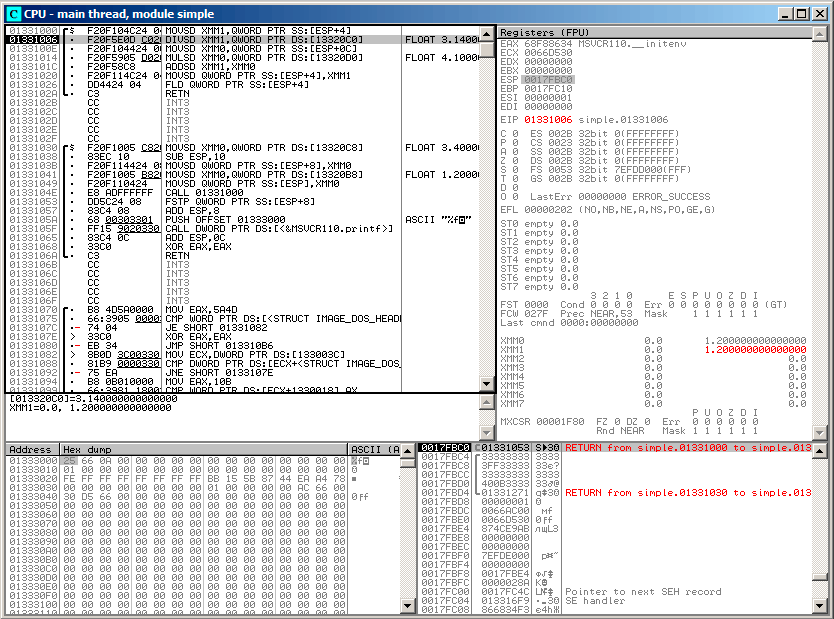
\includegraphics[scale=\FigScale]{patterns/205_floating_SIMD/simple_olly1.png}
\caption{\olly: \TT{MOVSD} \RU{загрузила значение}\EN{loads the value of} $a$ \RU{в}\EN{into} \XMM{1}}
\label{fig:FPU_SIMD_simple_olly1}
\end{figure}

\clearpage
\begin{figure}[H]
\centering
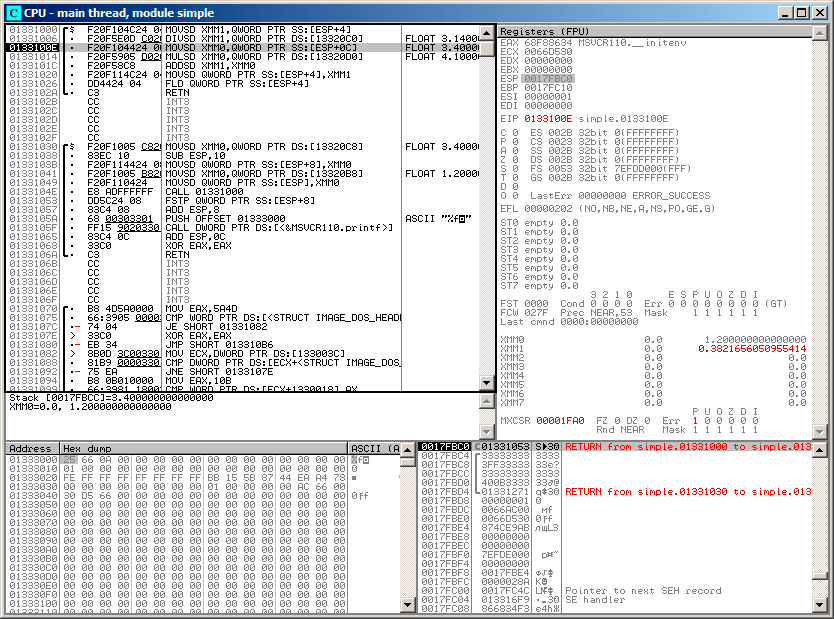
\includegraphics[scale=\FigScale]{patterns/205_floating_SIMD/simple_olly2.png}
\caption{\olly: \TT{DIVSD} \RU{вычислила}\EN{calculated} \gls{quotient} 
\RU{и оставила его в}\EN{and stored it in} \XMM{1}}
\label{fig:FPU_SIMD_simple_olly2}
\end{figure}

\clearpage
\begin{figure}[H]
\centering
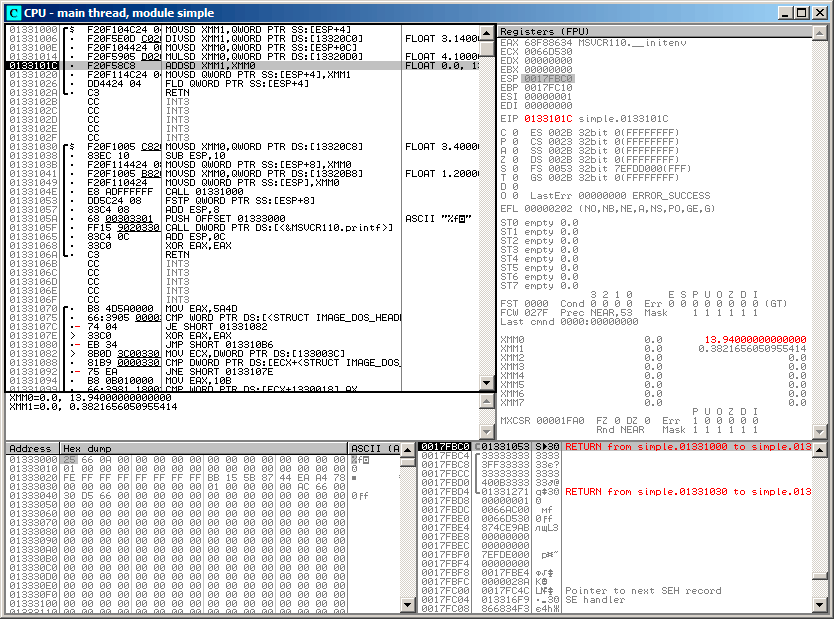
\includegraphics[scale=\FigScale]{patterns/205_floating_SIMD/simple_olly3.png}
\caption{\olly: \TT{MULSD} \RU{вычислила}\EN{calculated} \gls{product} \RU{и оставила его в}\EN{and stored it
in} \XMM{0}}
\label{fig:FPU_SIMD_simple_olly3}
\end{figure}

\clearpage
\begin{figure}[H]
\centering
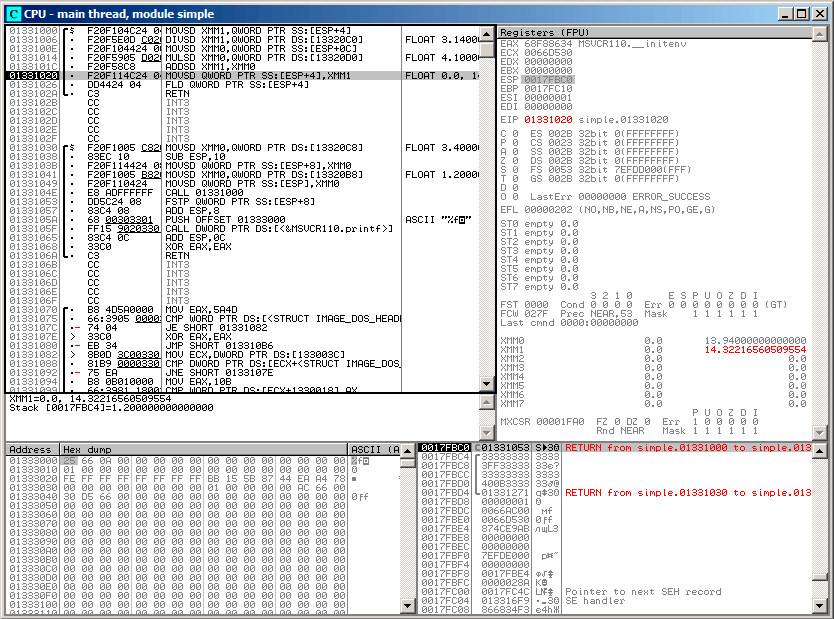
\includegraphics[scale=\FigScale]{patterns/205_floating_SIMD/simple_olly4.png}
\caption{\olly: \TT{ADDSD} \RU{прибавила значение в}\EN{adds value in} \XMM{0} \RU{к}\EN{to} \XMM{1}}
\label{fig:FPU_SIMD_simple_olly4}
\end{figure}

\clearpage
\begin{figure}[H]
\centering
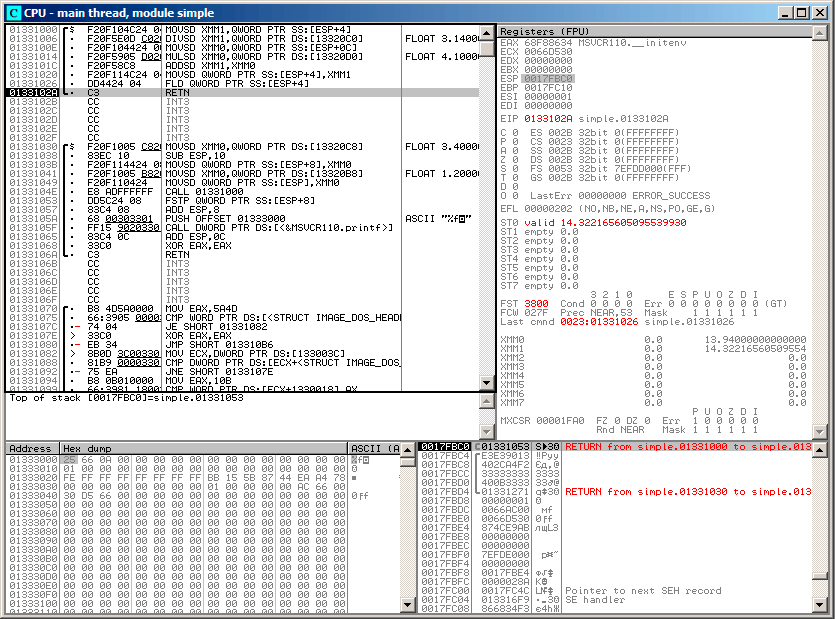
\includegraphics[scale=\FigScale]{patterns/205_floating_SIMD/simple_olly5.png}
\caption{\olly: \FLD \RU{оставляет результат функции в}\EN{left function result in} \ST{0}}
\label{fig:FPU_SIMD_simple_olly5}
\end{figure}

\RU{Видно, что \olly показывает XMM-регистры как пары чисел в формате \Tdouble,
но используется только \IT{младшая} часть.}
\EN{We see that \olly shows the XMM registers as pairs of \Tdouble numbers,
but only the \IT{lower} part is used.}
\RU{Должно быть, \olly показывает их именно так, потому что сейчас исполняются SSE2-инструкции
с суффиксом \TT{-SD}.}
\EN{Apparently, \olly shows them in that format because the SSE2 instructions (suffixed with \TT{-SD}) 
are executed right now.}
\RU{Но конечно же, можно переключить отображение значений в регистрах и посмотреть содержимое
как 4 \Tfloat{}-числа или просто как 16 байт.}
\EN{But of course, it's possible to switch the register format and to see their contents as
4 \Tfloat{}-numbers or just as 16 bytes.}
\fi

\clearpage
\section{\RU{Передача чисел с плавающей запятой в аргументах}\EN{Passing floating point number via arguments}}

\lstinputlisting{patterns/12_FPU/2_passing_floats/pow.c}

\RU{Они передаются в младших половинах регистров}\EN{They are passed in the lower halves
of the} \XMM{0}-\XMM{3}\EN{ registers}.

\lstinputlisting[caption=\Optimizing MSVC 2012 x64]{patterns/205_floating_SIMD/pow_MSVC_2012_x64_Ox.asm}

\index{x86!\Instructions!MOVSD}
\index{x86!\Instructions!MOVSDX}
\RU{Инструкции}\EN{There is no} \TT{MOVSDX} \RU{нет в документации от}\EN{instruction in} 
Intel \cite{Intel} \AndENRU AMD \cite{AMD}\EN{ manuals}, 
\RU{там она называется просто}\EN{there it is called just} \TT{MOVSD}.
\RU{Таким образом, в процессорах x86 две инструкции с одинаковым именем}\EN{So there are two instructions
sharing the same name in x86} (\RU{о второй}\EN{about the other see}: \myref{REP_MOVSx}).
\RU{Возможно, в Microsoft решили избежать
путаницы и переименовали инструкцию в}\EN{Apparently, Microsoft developers wanted to get rid of the mess,
so they renamed it to} \TT{MOVSDX}.
\RU{Она просто загружает значение в младшую половину XMM-регистра}\EN{It just loads a value into
the lower half of a XMM register}.

\RU{Функция }\TT{pow()} \RU{берет аргументы из}\EN{takes arguments from} \XMM{0} \AndENRU \XMM{1}, 
\RU{и возвращает результат в}\EN{and returns result in} \XMM{0}.
\RU{Далее он перекладывается в}\EN{It is then moved to} \RDX \ForENRU \printf. 
\RU{Почему}\EN{Why}? 
\RU{Может быть, это потому что}\EN{Maybe because} 
\printf\EMDASH{}\RU{функция с переменным количеством аргументов}\EN{is a variable arguments function}?

\lstinputlisting[caption=\Optimizing GCC 4.4.6 x64]{patterns/205_floating_SIMD/pow_GCC446_x64_O3.s.\LANG}

GCC \RU{работает понятнее}\EN{generates clearer output}. 
\RU{Значение для}\EN{The value for} \printf \RU{передается в}\EN{is passed in} \XMM{0}. 
\RU{Кстати, вот тот случай, когда в}\EN{By the way, here is a case when 1 is written into} \EAX
\ForENRU \printf \RU{записывается 1 --- это значит, что будет передан один аргумент в векторных регистрах, 
так того требует стандарт}\EN{---this implies that one argument will be passed in vector registers,
just as the standard requires} \cite{SysVABI}.

\section{\RU{Пример с сравнением}\EN{Comparison example}}

\lstinputlisting{patterns/12_FPU/3_comparison/d_max.c}

\subsection{x64}

\lstinputlisting[caption=\Optimizing MSVC 2012 x64]{patterns/205_floating_SIMD/d_max_MSVC_2012_x64_Ox.asm}

\Optimizing MSVC \RU{генерирует очень понятный код}\EN{generates a code very easy to understand}.

\index{x86!\Instructions!COMISD}
\RU{Инструкция }\TT{COMISD} \RU{это}\EN{is} \q{Compare Scalar Ordered Double-Precision Floating-Point 
Values and Set EFLAGS}. \RU{Собственно, это она и делает}\EN{Essentially, that is what it does}.\\
\\
\NonOptimizing MSVC \RU{генерирует более избыточно, но тоже всё понятно}\EN{generates more redundant code,
but it is still not hard to understand}:

\lstinputlisting[caption=MSVC 2012 x64]{patterns/205_floating_SIMD/d_max_MSVC_2012_x64.asm}

\index{x86!\Instructions!MAXSD}
\RU{А вот}\EN{However,} GCC 4.4.6 \RU{дошел в оптимизации дальше и применил инструкцию}
\EN{did more optimizations and used the} \TT{MAXSD} (\q{Return Maximum Scalar 
Double-Precision Floating-Point Value})\RU{, которая просто выбирает максимальное значение}\EN{ instruction,
which just choose the maximum value}!

\lstinputlisting[caption=\Optimizing GCC 4.4.6 x64]{patterns/205_floating_SIMD/d_max_GCC446_x64_O3.s}

\clearpage
\subsection{x86}

\RU{Скомпилируем этот пример в MSVC 2012 с включенной оптимизацией:}
\EN{Let's compile this example in MSVC 2012 with optimization turned on:}

\lstinputlisting[caption=\Optimizing MSVC 2012 x86]{patterns/205_floating_SIMD/d_max_MSVC_2012_x86_Ox.asm}

\RU{Всё то же самое, только значения}\EN{Almost the same, but the values of} $a$ \AndENRU $b$ 
\RU{берутся из стека, а результат функции оставляется в}\EN{are taken from the stack and the function result 
is left in} \ST{0}.

\ifdefined\IncludeOlly
\RU{Если загрузить этот пример в}\EN{If we load this example in} \olly, 
\RU{увидим, как инструкция}\EN{we can see how the} \TT{COMISD} \RU{сравнивает значения и устанавливает/сбрасывает
флаги}\EN{instruction compares values and sets/clears the} \CF \AndENRU \PF\EN{ flags}:

\begin{figure}[H]
\centering
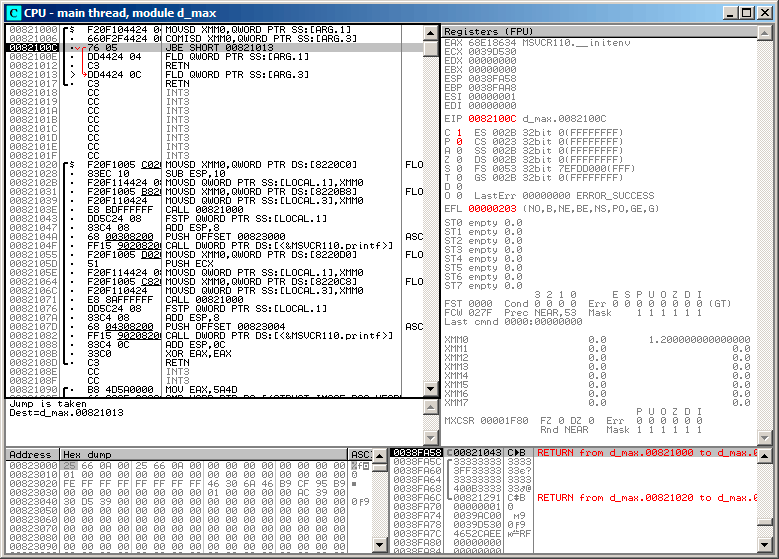
\includegraphics[scale=\FigScale]{patterns/205_floating_SIMD/d_max_olly.png}
\caption{\olly: \TT{COMISD} \RU{изменила флаги}\EN{changed} \CF \AndENRU \PF\EN{ flags}}
\label{fig:FPU_SIMD_d_max_olly}
\end{figure}
\fi

\section{\RU{Вычисление машинного эпсилона}\EN{Calculating machine epsilon}: x64 \AndENRU SIMD}
\label{machine_epsilon_x64_and_SIMD}

\RU{Вернемся к примеру \q{вычисление машинного эпсилона} для \Tdouble \lstref{machine_epsilon_double_c}.}
\EN{Let's revisit the \q{calculating machine epsilon} example for \Tdouble \lstref{machine_epsilon_double_c}.}

\RU{Теперь скомпилируем его для x64}\EN{Now we compile it for x64}:

\lstinputlisting[caption=\Optimizing MSVC 2012 x64]{patterns/205_floating_SIMD/epsilon_double_MSVC_2012_x64_Ox.asm}

\RU{Нет способа прибавить 1 к значению в 128-битном XMM-регистре, так что его нужно в начале поместить в память.}
\EN{There is no way to add 1 to a value in 128-bit XMM register, so it must be placed into memory.}

\RU{Впрочем, есть инструкция ADDSD (\IT{Add Scalar Double-Precision Floating-Point Values}),
которая может прибавить значение к младшей 64-битной части XMM-регистра игнорируя старшую половину,
но наверное MSVC 2012 пока недостаточно хорош для этого}
\EN{There is, however, the ADDSD instruction (\IT{Add Scalar Double-Precision Floating-Point Values}) 
which can add a value to the lowest 64-bit half of a XMM register while ignoring the higher one, 
but MSVC 2012 probably is not that good yet}
\footnote{\RU{В качестве упражнения, вы можете попробовать переработать этот код, чтобы избавиться 
от использования локального стека}\EN{As an exercise, you may try to rework this code to 
eliminate the usage of the local stack}.}.

\RU{Так или иначе, значение затем перезагружается в XMM-регистр и происходит вычитание.}
\EN{Nevertheless, the value is then reloaded to a XMM register and subtraction occurs.}
SUBSD \RU{это}\EN{is} \q{Subtract Scalar Double-Precision Floating-Point Values}, 
\RU{т.е. операция производится над младшей 64-битной частью 128-битного XMM-регистра}
\EN{i.e., it operates on the lower 64-bit part of 128-bit XMM register}.
\RU{Результат возвращается в регистре XMM0}\EN{The result is returned in the XMM0 register}.

\input{patterns/205_floating_SIMD/FPU_PRNG/main}

\section{\RU{Итог}\EN{Summary}}

\RU{Во всех приведенных примерах, в XMM-регистрах используется только младшая половина регистра, там
хранится значение в формате IEEE 754}\EN{Only the lower half of XMM registers is used in all examples here, 
to store number in IEEE 754 format}.

\RU{Собственно, все инструкции с суффиксом}\EN{Essentially, all instructions prefixed by} 
\TT{-SD} (\q{Scalar Double-Precision})\EMDASH{}\RU{это инструкции для работы с числами с плавающей 
запятой в формате IEEE 754, 
хранящиеся в младшей 64-битной половине XMM-регистра}\EN{are instructions working with floating point numbers
in IEEE 754 format, stored in the lower 64-bit half of a XMM register}.

\RU{Всё удобнее чем это было в FPU, видимо, сказывается тот факт, что расширения 
SIMD развивались не так хаотично как FPU в прошлом.}
\EN{And it is easier than in the FPU, probably because the SIMD extensions 
were evolved in a less chaotic way than the FPU ones in the past.}
\RU{Стековая модель регистров не используется}\EN{The stack register model is not used}.

\index{x86!\Instructions!ADDSS}
\index{x86!\Instructions!MOVSS}
\index{x86!\Instructions!COMISS}
% TODO1: do this!
\RU{Если вы попробуете заменить в этих примерах}\EN{If you would try to replace} \Tdouble \RU{на}\EN{with} \Tfloat
\RU{, то инструкции будут использоваться те же,
только с суффиксом}
% FIXME1 ... but their -SS versions
\EN{in these examples, the same instructions will be used, but prefixed with} \TT{-SS} 
(\q{Scalar Single-Precision}), \RU{например}\EN{for example}, \TT{MOVSS}, \TT{COMISS}, \TT{ADDSS}, \etc{}.

\q{Scalar} \RU{означает что SIMD-регистр будет хранить только одно значение, вместо нескольких.}
\EN{implies that the SIMD register containing only one value instead of several.}
\RU{Инструкции, работающие с несколькими значениями в регистре одновременно, имеют \q{Packed} в названии}
\EN{Instructions working with several values in a register simultaneously have \q{Packed} in their name}.

\RU{Нужно также обратить внимание, что SSE2-инструкции работают с 64-битными числами (\Tdouble) в формате IEEE 754,
в то время как внутреннее представление в FPU --- 80-битные числа.}
\EN{Needless to say, the SSE2 instructions work with 64-bit IEEE 754 numbers (\Tdouble),
while the internal representation of the floating-point numbers in FPU is 80-bit numbers.}
\RU{Поэтому ошибок округления (\IT{round-off error}) в FPU может быть меньше чем в SSE2,
как следствие, можно сказать, работа с FPU может давать более точные результаты вычислений.}
\EN{Hence, the FPU may produce less round-off errors and as a consequence, FPU may give more precise
calculation results.}

\fi
\ifdefined\IncludeARM
\chapter{\EN{ARM-specific details}\RU{Кое-что специфичное для ARM}}

\section{\RU{Знак номера}\EN{Number sign} (\#) \RU{перед числом}\EN{before number}}

\RU{Компилятор Keil, \IDA и objdump предваряет все числа знаком номера (\q{\#}), например:}
\EN{The Keil compiler, \IDA and objdump precede all numbers with the \q{\#} number sign, for example:}
\lstref{Keil_number_sign}.
\RU{Но когда GCC 4.9 выдает результат на языке ассемблера, он так не делает, например:}
\EN{But when GCC 4.9 generates assembly language output, it doesn't, for example: }
\lstref{GCC_no_number_sign}.

\RU{Так что листинги для ARM в этой книге в каком-то смысле перемешаны.}
\EN{The ARM listings in this book are somewhat mixed.}

\RU{Трудно сказать, как правильнее.}\EN{It's hard to say, which method is right.}
\RU{Должно быть, всякий должен придерживаться тех правил, которые приняты в той среде, в которой он работает.}%
\EN{Supposedly, one has to obey the rules accepted in environment he/she works in.}

% sections
\input{patterns/ARM/post_pre_index.tex}
\input{patterns/ARM/big_constants.tex}
\input{patterns/ARM/relocs.tex}

\fi
\ifdefined\IncludeMIPS
\chapter{\EN{MIPS-specific details}\RU{Кое-что специфичное для MIPS}}

% sections
\input{patterns/MIPS/big_constants.tex}

\section{\RU{Книги и прочие материалы о MIPS}\EN{Further reading about MIPS}}

\cite{MIPSRun}.

\fi

\part{\RU{Важные фундаментальные вещи}\EN{Important fundamentals}}

\clearpage
\begin{center}
\vspace*{\fill}

\begin{figure}[H]
\centering
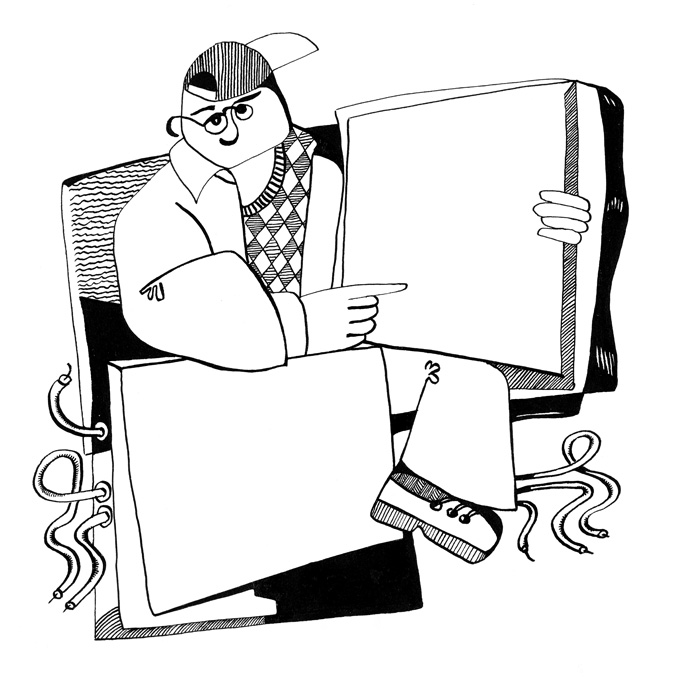
\includegraphics[scale=\FigScale]{cover2.jpg}
\end{figure}

\vspace*{\fill}
\end{center}

\clearpage

% chapters
\chapter{\SignedNumbersSectionName}
\label{sec:signednumbers}
\index{Signed numbers}

\newcommand{\URLS}{\href{http://go.yurichev.com/17117}{wikipedia}}

\RU{Методов представления чисел с знаком \q{плюс} или \q{минус} несколько\footnote{\URLS}, 
но в компьютерах обычно применяется метод \q{дополнительный код} или \q{two's complement}.}
\EN{There are several methods for representing signed numbers\footnote{\URLS}, 
but \q{two's complement} is the most popular one in computers.}

\EN{Here is a table for some byte values:}
\RU{Вот таблица некоторые значений байтов:}

\begin{center}
\begin{tabular}{ | l | l | l | l | }
\hline
\cellcolor{blue!25} \RU{двоичное}\EN{binary} & 
\cellcolor{blue!25} \RU{шестнадцатеричное}\EN{hexadecimal} & 
\cellcolor{blue!25} \RU{беззнаковое}\EN{unsigned} &
\cellcolor{blue!25} \RU{знаковое}\EN{signed} (\RU{дополнительный код}\EN{2's complement}) \\
\hline
01111111 & 0x7f & 127 & 127 \\
\hline
01111110 & 0x7e & 126 & 126 \\
\hline
\multicolumn{4}{ |c| }{...} \\
\hline
00000110 & 0x6 & 6 & 6 \\
\hline
00000101 & 0x5 & 5 & 5 \\
\hline
00000100 & 0x4 & 4 & 4 \\
\hline
00000011 & 0x3 & 3 & 3 \\
\hline
00000010 & 0x2 & 2 & 2 \\
\hline
00000001 & 0x1 & 1 & 1 \\
\hline
00000000 & 0x0 & 0 & 0 \\
\hline
11111111 & 0xff & 255 & -1 \\
\hline
11111110 & 0xfe & 254 & -2 \\
\hline
11111101 & 0xfd & 253 & -3 \\
\hline
11111100 & 0xfc & 252 & -4 \\
\hline
11111011 & 0xfb & 251 & -5 \\
\hline
11111010 & 0xfa & 250 & -6 \\
\hline
\multicolumn{4}{ |c| }{...} \\
\hline
10000010 & 0x82 & 130 & -126 \\
\hline
10000001 & 0x81 & 129 & -127 \\
\hline
10000000 & 0x80 & 128 & -128 \\
\hline
\end{tabular}
\end{center}

\index{x86!\Instructions!JA}
\index{x86!\Instructions!JB}
\index{x86!\Instructions!JL}
\index{x86!\Instructions!JG}
\RU{Разница в подходе к знаковым/беззнаковым числам, собственно, нужна потому что, например, 
если представить \TT{0xFFFFFFFE} и \TT{0x0000002} как беззнаковое, то первое число (4294967294) больше второго (2). 
Если их оба представить как знаковые, то первое будет $-2$, которое, разумеется, меньше чем второе (2).
Вот почему инструкции для условных переходов~(\myref{sec:Jcc}) представлены в обоих версиях ~--- 
и для знаковых сравнений (например, \JG, \JL) и для беззнаковых (\JA, \JB).}
\EN{The difference between signed and unsigned numbers is that if we represent \TT{0xFFFFFFFE} and \TT{0x0000002} 
as unsigned, then the first number (4294967294) is bigger than the second one (2). 
If we represent them both as signed, the first one is to be $-2$, and it is smaller than the second (2). 
That is the reason why conditional jumps~(\myref{sec:Jcc}) are present both for signed (e.g. \JG, \JL) 
and unsigned (\JA, \JB) operations.}\PTBRph{}\ESph{}\PLph{} \\
\\
\RU{Для простоты, вот что нужно знать}\EN{For the sake of simplicity, that is what one need to know}:
\begin{itemize}
\item \RU{Числа бывают знаковые и беззнаковые}\EN{Numbers can be signed or unsigned}.

\item \RU{Знаковые типы в \CCpp}\EN{\CCpp signed types}:
  \begin{itemize}
    \item \TT{int64\_t} (-9,223,372,036,854,775,808..9,223,372,036,854,775,807) (-~9.2..~9.2 \EN{quintillions}\RU{квинтиллионов}) \OrENRU \\
                \TT{0x8000000000000000..0x7FFFFFFFFFFFFFFF}),
    \item \Tint (-2,147,483,648..2,147,483,647 (-~2.15..~2.15Gb) \OrENRU \TT{0x80000000..0x7FFFFFFF}),
    \item \Tchar (-128..127 \OrENRU \TT{0x80..0x7F}),
    \item \TT{ssize\_t}.
   \end{itemize}

	\RU{Беззнаковые}\EN{Unsigned}: 
  \begin{itemize}
	  \item \TT{uint64\_t} (0..18,446,744,073,709,551,615 (~18 \EN{quintillions}\RU{квинтиллионов}) \OrENRU \TT{0..0xFFFFFFFFFFFFFFFF}),
   \item \TT{unsigned int} (0..4,294,967,295 (~4.3Gb) \OrENRU \TT{0..0xFFFFFFFF}),
   \item \TT{unsigned char} (0..255 \OrENRU \TT{0..0xFF}), 
   \item \TT{size\_t}.
  \end{itemize}

\item \RU{У знаковых чисел знак определяется самым старшим битом: 1 означает \q{минус}, 0 означает \q{плюс}}
	\EN{Signed types have the sign in the most significant bit: 1 mean \q{minus}, 0 mean \q{plus}}.

\item \EN{Promoting to a larger data types is simple:}
      \RU{Преобразование в б\'{о}льшие типы данных обходится легко:} \myref{subsec:sign_extending_32_to_64}.

\label{sec:signednumbers:negation}
\item \EN{Negation is simple: just invert all bits and add 1.}
\RU{Изменить знак легко: просто инвертируйте все биты и прибавьте 1.}
\EN{We can remember that a number of inverse sign is located 
on the opposite side at the same proximity from zero.}
\RU{Мы можем заметить, что число другого знака находится на другой стороне на том же расстоянии от нуля.}
\RU{Прибавление единицы необходимо из-за присутствия нуля посредине.}
\EN{The addition of one is needed because zero is present in the middle.}

\index{x86!\Instructions!IDIV}
\index{x86!\Instructions!DIV}
\index{x86!\Instructions!IMUL}
\index{x86!\Instructions!MUL}
\index{x86!\Instructions!CBW}
\index{x86!\Instructions!CWD}
\index{x86!\Instructions!CWDE}
\index{x86!\Instructions!CDQ}
\index{x86!\Instructions!CDQE}
\index{x86!\Instructions!MOVSX}
\index{x86!\Instructions!SAR}
\item \RU{Инструкции сложения и вычитания работают одинаково хорошо и для знаковых и для беззнаковых значений}
	\EN{The addition and subtraction operations work well for both signed and unsigned values}.
	\RU{Но для операций умножения и деления, в x86 имеются разные инструкции}
	\EN{But for multiplication and division operations, x86 has different instructions}:
	\TT{IDIV}/\TT{IMUL} \RU{для знаковых}\EN{for signed}
	\AndENRU \TT{DIV}/\TT{MUL} \RU{для беззнаковых}\EN{for unsigned}.
\ifx\LITE\undefined
\item \RU{Еще инструкции работающие с знаковыми числами}\EN{Here are some more instructions that work with signed numbers}:
	\TT{CBW/CWD/CWDE/CDQ/CDQE} (\myref{ins:CBW_CWD_etc}), \TT{MOVSX} (\myref{MOVSX}), \TT{SAR} (\myref{ins:SAR}).
\fi
\end{itemize}

\iffalse
% TODO rework!
\section{\RU{Переполнение integer}\EN{Integer overflow}}

\RU{Бывает так, что ошибки представления знаковых/беззнаковых могут привести к уязвимости 
\IT{переполнение integer}.}
\EN{It is worth noting that the incorrect representation of a number can lead to integer overflow vulnerabilities.}

\RU{Например, есть некий сервис, который принимает по сети некие пакеты. 
В пакете есть заголовок где указана длина пакета. Это 32-битное значение. 
В процессе приема пакета, 
сервис проверяет это значение и сверяет, больше ли оно чем максимальный размер пакета, скажем, константа
\TT{MAX\_PACKET\_SIZE} (например, 10 килобайт), и если да, то пакет отвергается как некорректный. 
Сравнение знаковое. Злоумышленник подставляет значение \TT{0xFFFFFFFF}. Это число трактуется как знаковое $-1$ 
и оно меньше чем 10000. Проверка проходит. Продолжаем дальше и копируем этот пакет куда-нибудь себе 
в сегмент данных\dots вызов функции \TT{memcpy (dst, src, 0xFFFFFFFF)} скорее всего, 
затрет много чего внутри процесса.}
\EN{For example, we have a network service and it receives network packets. 
In the packets there is a field where the subpacket length is encoded. 
It is a 32-bit value. 
After the receiving of the network packet, the service checks the field and if it is larger than 
some \TT{MAX\_PACKET\_SIZE} (let's say, 10 kilobytes), the packet is rejected as incorrect.
The comparison is signed. The intruder set this value to \TT{0xFFFFFFFF}.
While comparing, this number is considered as signed $-1$ and it is less than 10 kilobytes. 
No error here. 
The service would then like to copy the subpacket to another place in memory and calls the 
\TT{memcpy (dst, src, 0xFFFFFFFF)} function: this operation, rapidly garbles a lot of 
of process memory.}

\RU{Немного подробнее}\EN{More about it}: \cite{Phrack3C0A}.
% TODO example!
\fi

\ifx\LITE\undefined
\chapter{Endianness\RU{ (порядок байт)}}
\label{sec:endianness}

\RU{Endianness (порядок байт) это способ представления чисел в памяти}
\EN{The endianness is a way of representing values in memory}.

\section{Big-endian\RU{ (от старшего к младшему)}}

\RU{Число}\EN{The} \TT{0x12345678} \RU{представляется в памяти так}
\EN{value is represented in memory as}:

\begin{center}
\begin{tabular}{ | l | l | }
\hline
\cellcolor{blue!25} \RU{адрес в памяти}\EN{address in memory} & \cellcolor{blue!25} \RU{значение байта}\EN{byte value} \\
\hline
+0 & 0x12 \\
\hline
+1 & 0x34 \\
\hline
+2 & 0x56 \\
\hline
+3 & 0x78 \\
\hline
\end{tabular}
\end{center}

\RU{CPU с таким порядком включают в себя}\EN{Big-endian CPUs include} Motorola 68k, IBM POWER.

\section{Little-endian\RU{ (от младшего к старшему)}}

\RU{Число}\EN{The} \TT{0x12345678} 
\RU{представляется в памяти так}
\EN{value is represented in memory as}:

\begin{center}
\begin{tabular}{ | l | l | }
\hline
\cellcolor{blue!25} \RU{адрес в памяти}\EN{address in memory} & \cellcolor{blue!25} \RU{значение байта}\EN{byte value} \\
\hline
+0 & 0x78 \\
\hline
+1 & 0x56 \\
\hline
+2 & 0x34 \\
\hline
+3 & 0x12 \\
\hline
\end{tabular}
\end{center}

\RU{CPU с таким порядком байт включают в себя}\EN{Little-endian CPUs include} Intel x86.

\section{\Example}

\RU{Возьмем big-endian Linux для MIPS заинсталированный в QEMU}%
\EN{Let's take big-endian MIPS Linux installed and ready in QEMU}
\footnote{\RU{Доступен для скачивания здесь}\EN{Available for download here}: \url{http://go.yurichev.com/17008}}.

\RU{И скомпилируем этот простой пример}\EN{And let's compile this simple example}:

\begin{lstlisting}
#include <stdio.h>

int main()
{
	int v, i;

	v=123;

	printf ("%02X %02X %02X %02X\n", 
		*(char*)&v,
		*(((char*)&v)+1),
		*(((char*)&v)+2),
		*(((char*)&v)+3));
};
\end{lstlisting}

\RU{И запустим его}\EN{And after running it we get}:

\begin{lstlisting}
root@debian-mips:~# ./a.out 
00 00 00 7B
\end{lstlisting}

\RU{Это оно и есть}\EN{That is it}.
0x7B \RU{это}\EN{is} 123 \RU{в десятичном виде}\EN{in decimal}.
\RU{В little-endian-архитектуре, 7B это первый байт (вы можете это проверить в x86 или x86-64),
но здесь он последний, потому что старший байт идет первым.}
\EN{In little-endian architectures, 7B is the first byte (you can check on x86 or x86-64), 
but here it is the last one, because the highest byte goes first.}

\RU{Вот почему имеются разные дистрибутивы Linux для MIPS}
\EN{That's why there are separate Linux distributions for MIPS} 
(\q{mips} (big-endian) \AndENRU \q{mipsel} (little-endian)).
\RU{Программа скомпилированная для одного соглашения об endiannes, не сможет работать в OS использующей
другое соглашение.}
\EN{It is impossible for a binary compiled for one endianness to work on an OS with different endianness.}\\
\\
\RU{Еще один пример связанный с big-endian в MIPS в этой книге:}
\EN{There is another example of MIPS big-endiannes in this book:} \myref{MIPS_structure_big_endian}.

\section{Bi-endian\RU{ (переключаемый порядок)}}

\RU{CPU поддерживающие оба порядка, и его можно переключать, включают в себя}
\EN{CPUs that may switch between endianness are} ARM, PowerPC, SPARC, MIPS, \ac{IA64}, \etc{}.

\section{\RU{Конвертирование}\EN{Converting data}}

\index{x86!\Instructions!BSWAP}
\RU{Инструкция }{The }\TT{BSWAP} \RU{может использоваться для конвертирования}
\EN{instruction can be used for conversion}.

\index{TCP/IP}
\RU{Сетевые пакеты TCP/IP используют соглашение big-endian, вот почему программа, работающая на little-endian архитектуре
должна конвертировать значения.}
\EN{TCP/IP network data packets use the big-endian conventions, so that is why a program working on a little-endian architecture
has to convert the values.} 

\RU{Обычно, используются функции}\EN{The} \TT{htonl()} \AndENRU \TT{htons()}\EN{ functions are usually used}.

\RU{Порядок байт big-endian в среде TCP/IP также называется}
\EN{In TCP/IP, big-endian is also called} \q{network byte order},
\RU{а порядок байт на компьютере}\EN{while byte order on the computer}\EMDASH{}\q{host byte order}.
\RU{На архитектуре Intel x86, и других little-endian архитектурах, \q{host byte order} это little-endian, 
а вот на IBM POWER это может быть big-endian, так что на последней, 
\TT{htonl()} и \TT{htons()} не меняют порядок байт.}
\EN{\q{host byte order} is little-endian on Intel x86 and other little-endian architectures,
but it is big-endian on IBM POWER, so \TT{htonl()} and \TT{htons()} are not shuffle any bytes
on latter.}

\fi
\chapter{\RU{Память}\EN{Memory}}

\RU{Есть три основных типа памяти:}
\EN{There are 3 main types of memory:}

\begin{itemize}
\item \RU{Глобальная память}\EN{Global memory}.
\ac{AKA} \q{static memory allocation}.
\RU{Нет нужды явно выделять, выделение происходит просто при объявлении переменных/массивов 
глобально.}
\EN{No need to allocate explicitly, the allocation is done just by declaring variables/arrays 
globally.}
\RU{Это глобальные переменные расположенные в сегменте данных или констант.}
\EN{These are global variables, residing in the data or constant segments.}
\RU{Доступны глобально (поэтому считаются \glslink{anti-pattern}{анти-паттерном}).}
\EN{The are available globally (hence, considered as an \gls{anti-pattern}).}
\RU{Не удобны для буферов/массивов, потому что должны иметь фиксированный размер.}
\EN{Not convenient for buffers/arrays, because they must have a fixed size.}
\RU{Переполнения буфера, случающиеся здесь, обычно перезаписывают переменные или буферы
расположенные рядом в памяти.}
\EN{Buffer overflows that occur here usually overwrite variables or buffers reside next to them in memory.}
\RU{Пример в этой книге}\EN{There's an example in this book}: \myref{scanf_global_variable}.

\item \RU{Стек}\EN{Stack}.
\ac{AKA} \q{allocate on stack}\RU{, \q{выделить память в/на стеке}}.
\RU{Выделение происходит просто при объявлении переменных/массивов локально в функции.}
\EN{The allocation is done just by declaring variables/arrays locally in the function.}
\RU{Обычно это локальные для функции переменные}\EN{These are usually local variables for the function}.
\RU{Иногда эти локальные переменные также доступны и для нисходящих функций (\gls{callee}-функциям, если функция-\gls{caller} передает
указатель на переменную в функцию-\gls{callee}).}
\EN{Sometimes these local variable are also available to descending functions 
(to \gls{callee} functions, if caller passes a pointer to a variable to the \gls{callee} to be executed).}
\RU{Выделение и освобождение очень быстрое, достаточно просто сдвига \ac{SP}.}
\EN{Allocation and deallocation are very fast, it's just \ac{SP} needs to be shifted.}
\index{\CStandardLibrary!alloca()}
\EN{But they're also not convenient for buffers/arrays, because the buffer size has to be fixed,
unless \TT{alloca()} (\myref{alloca}) (or a variable-length array) is used.}
\RU{Но также не удобно для буферов/массивов, потому что размер буфера фиксирован,
если только не используется \TT{alloca()} (\myref{alloca}) (или массив с переменной длиной).}
\RU{Переполнение буфера обычно перезаписывает важные структуры стека}\EN{Buffer overflows usually 
overwrite important stack structures}: \myref{subsec:bufferoverflow}.

\index{\CStandardLibrary!malloc()}
\index{\CStandardLibrary!free()}
\item \RU{Куча (\IT{heap})}\EN{Heap}. 
\ac{AKA} \q{dynamic memory allocation}\RU{, \q{выделить память в куче}}.
\RU{Выделение происходит при помощи вызова}\EN{Allocation is done by calling} 
\TT{malloc()/free()} \OrENRU \TT{new/delete} \InENRU \Cpp.
\RU{Самый удобный метод: размер блока может быть задан во время исполнения}\EN{This is the most convenient 
method: the block size may be set at runtime}.
\index{\CStandardLibrary!realloc()}
\RU{Изменение размера возможно (при помощи \TT{realloc()}), но может быть медленным.}
\EN{Resizing is possible (using \TT{realloc()}), but can be slow.}
\RU{Это самый медленный метод выделения памяти: аллокатор памяти должен поддерживать и обновлять
все управляющие структуры во время выделения и освобождения.}
\EN{This is the slowest way to allocate memory: 
the memory allocator must support and update all control structures while
allocating and deallocating.}
\RU{Переполнение буфера обычно перезаписывает все эти структуры}\EN{Buffer overflows usually 
overwrite these structures}.
\RU{Выделения в куче также ведут к проблеме утечек памяти: каждый выделенный блок должен быть
явно освобожден, но кто-то может забыть об этом, или делать это неправильно.}
\EN{Heap allocations are also source of memory leak problems: each memory block has to be deallocated
explicitly, but one may forget about it, or do it incorrectly.}
\index{\CStandardLibrary!free()}
\RU{Еще одна проблема --- это \q{использовать после освобождения} --- использовать блок памяти после
того как \TT{free()} был вызван на нем, это тоже очень опасно.}
\EN{Another problem is the \q{use after free}---using a memory block after \TT{free()} was called on it,
which is very dangerous.}
\RU{Пример в этой книге}\EN{Example in this book}: \myref{struct_malloc_example}.

\end{itemize}

\ifx\LITE\undefined
\chapter{CPU}

\section{\RU{Предсказатели переходов}\EN{Branch predictors}}
\label{branch_predictors}

\RU{Некоторые современные компиляторы пытаются избавиться от инструкций условных переходов}\EN{Some modern 
compilers try to get rid of conditional jump instructions}.
\RU{Примеры в этой книге}\EN{Examples in this book are}: 
\myref{subsec:jcc_ARM}, \myref{chap:cond}, \myref{subsec:popcnt}.

\RU{Это потому что предсказатель переходов далеко не всегда работает идеально, поэтому, компиляторы и стараются
реже использовать переходы, если возможно.}
\EN{This is because the branch predictor is not always perfect, so the compilers try to do 
without conditional jumps, if possible.}

\index{x86!\Instructions!CMOVcc}
\index{ARM!\Instructions!ADRcc}
\RU{Одна из возможностей --- это условные инструкции в ARM (как ADRcc), а еще инструкция CMOVcc в x86.}
\EN{Conditional instructions in ARM (like ADRcc) are one way, another one is the CMOVcc x86 instruction.}

\section{\RU{Зависимости между данными}\EN{Data dependencies}}

\EN{Modern CPUs are able to execute instructions simultaneously (\ac{OOE}), but in order to do so,
the results of one instruction in a group must not influence the execution of others.}
\RU{Современные процессоры способны исполнять инструкции одновременно (\ac{OOE}), но для этого,
внутри такой группы, результат одних не должен влиять на работу других.}
\EN{Hence, the compiler endeavors to use instructions with minimal influence to the CPU state.}
\RU{Следовательно, компилятор старается использовать инструкции с наименьшим влиянием на
состояние процессора.}

\EN{That's why the \LEA instruction is so popular, because it does not modify CPU flags, while
other arithmetic instructions does.}
\RU{Вот почему инструкция \LEA в x86 такая популярная --- 
потому что она не модифицирует флаги процессора,
а прочие арифметические инструкции --- модифицируют.}

\newcommand{\HashFuncChapterName}{\RU{Хеш-функции}\EN{Hash functions}}
\chapter{\HashFuncChapterName}
\label{hash_func}

\index{\HashFuncChapterName}
\index{CRC32}
\RU{Простейший пример это CRC32, алгоритм \q{более мощный} чем простая контрольная сумма,
для проверки целостности данных}
\EN{A very simple example is CRC32, an algorithm that provides \q{stronger} checksum for integrity checking purposes}.
\RU{Невозможно восстановить оригинальный текст из хеша, там просто меньше информации: ведь текст
может быть очень длинным, но результат CRC32 всегда ограничен 32 битами}
\EN{it is impossible to restore the original text from the hash value, it has much less information:
the input can be long, but CRC32's result is always limited to 32 bits}.
\RU{Но CRC32 не надежна в криптографическом смысле: известны методы как изменить текст таким образом,
чтобы получить нужный результат.}
\EN{But CRC32 is not cryptographically secure: it is known how to alter a text in a way that the resulting
CRC32 hash value will be the one we need.}
\RU{Криптографические хеш-функции защищены от этого}
\EN{Cryptographic hash functions are protected from this}.\\
\\
\index{MD5}
\index{SHA1}
\RU{Такие функции как MD5, SHA1, \etc{}., широко используются для хеширования паролей
для хранения их в базе}
\EN{Such functions are MD5, SHA1, \etc{}, and they are widely used to hash user passwords in order to store them in a database}.
\RU{Действительно: БД форума в интернете может и не хранить пароли 
(иначе злоумышленник получивший доступ к БД сможет узнать все пароли), а только хеши}
\EN{Indeed: an internet forum database may not contain user passwords 
(a stolen database can compromise all user's passwords) but only hashes 
(a cracker can't reveal passwords)}.
\RU{К тому же, скрипту интернет-форума вовсе не обязательно знать ваш пароль, он только должен
сверить его хеш с тем что лежит в БД, и дать вам доступ если cверка проходит}
\EN{Besides, an internet forum engine is not aware of your password, it has only to check if its hash
is the same as the one in the database, and give you access if they match}.
\RU{Один из самых простых способов взлома --- это просто перебирать все пароли и ждать пока
результат будет такой же как тот что нам нужен.}
\EN{One of the simplest password cracking methods is just to try hashing all possible passwords in order
to see which is matching the resulting value that we need.}
\RU{Другие методы намного сложнее}\EN{Other methods are much more complex}.
% TODO1 add about Rainbow tables

\section{\RU{Как работает односторонняя функция}\EN{How one-way function works}?}

\RU{Односторонняя функция, это функция, которая способна превратить из одного значения другое,
при этом невозможно (или трудно) проделать обратную операцию.}
\EN{One-way function is a function which is able to transform one value into another,
while it is impossible (or very hard) to do reverse it back.}
\RU{Некоторые люди имеют трудности с пониманием, как это возможно.}
\EN{Some people have difficulties while understanding how it's possible at all.}
\RU{Рассмотрим очень простой пример.}\EN{Let's consider simple demonstration.}

\RU{У нас есть ряд из 10-и чисел в пределах 0..9, каждое встречается один раз, например:}%
\EN{We've got vector of 10 numbers in range 0..9, each encounters only once, for example:}

\begin{lstlisting}
4 6 0 1 3 5 7 8 9 2
\end{lstlisting}

\RU{Алгоритм простейшей односторонней функции выглядит так}\EN{Algorithm of simplest possible one-way function is}:

\begin{itemize}
\item \RU{возьми число на нулевой позиции (у нас это 4)}\EN{take a number at zeroth position (4 in our case)};
\item \RU{возьми число на первой позиции (у нас это 6)}\EN{take a number at first position (6 in our case)};
\item \RU{обменяй местами числа на позициях 4 и 6}\EN{swap numbers at positions of  4 and 6}.
\end{itemize}

\RU{Отметим числа на позициях 4 и 6}\EN{Let's mark numbers on positions of 4 and 6}:

\begin{lstlisting}
4 6 0 1 3 5 7 8 9 2
        ^   ^
\end{lstlisting}

\RU{Меняем их местами и получаем результат}\EN{Let's swap them and we've got a result}:

\begin{lstlisting}
4 6 0 1 7 5 3 8 9 2
\end{lstlisting}

\RU{Глядя на результат, и даже зная алгоритм функции, мы не можем однозначно восстановить изначальное
положение чисел.
Ведь первые два числа могли быть 0 и/или 1, и тогда именно они могли бы участвовать в обмене.}
\EN{While looking at the result and even if we know algorithm, we can't say unambiguously initial
numbers set.
Because first two numbers could be 0 and/or 1, and then they could be participate in swapping
procedure.}

\RU{Это крайне упрощенный пример для демонстрации, настоящие односторонние функции могут быть значительно
сложнее.}
\EN{This is utterly simplified example for demonstration, real one-way functions may be much more
complex.}

\fi

\ifx\LITE\undefined
\part{\EN{Slightly more advanced examples}\RU{Более сложные примеры}}

\newcommand{\CURPATH}{advanced/100_fahrenheit}
\section{\RU{Указатель на аргумент функции}\EN{Taking a pointer to function argument}}
\label{pointer_to_argument}

\dots \RU{и даже более того, можно взять указатель на аргумент функции и передать его в другую функцию:}
\EN{even more than that, it's possible to take a pointer to the function's argument and pass
it to another function:}

\lstinputlisting{OS/calling_conventions/ptr_to_argument/10.c}

\RU{Трудно понять, как это работает, пока мы не посмотрим на код:}
\EN{It's hard to understand how it works until we can see the code:}

\lstinputlisting[caption=\Optimizing MSVC 2010]{OS/calling_conventions/ptr_to_argument/MSVC_2010_O3.asm}

\RU{Адрес места в стеке где была передана $a$ просто передается в другую функцию.
Она модифицирует переменную по этому адресу, и затем \printf выведет модифицированное значение.}
\EN{The address of the place in the stack where $a$ was passed is just passed to another function.
It modifies the value addressed by the pointer and then \printf prints the modified value.}\ESph{}\PTBRph{}\PLph{}\\
\\
\RU{Наблюдательный читатель может спросить, а что насчет тех соглашений о вызовах, где аргументы функции
передаются в регистрах?}
\EN{The observant reader might ask, what about calling conventions where the function's arguments are
passed in registers?}

\RU{Это та ситуация где используется \IT{Shadow Space}.}
\EN{That's a situation where the \IT{Shadow Space} is used.}
\RU{Так что входящее значение копируется из регистра в \IT{Shadow Space} в локальном стеке и затем это адрес
передается в другую функцию:}
\EN{The input value is copied from the register
to the \IT{Shadow Space} in the local stack, and then this address is passed to the other function:}

\lstinputlisting[caption=\Optimizing MSVC 2012 x64]{OS/calling_conventions/ptr_to_argument/MSVC_2012_x64_O3.asm}

\RU{GCC также записывает входное значение в локальный стек:}
\EN{GCC also stores the input value in the local stack:}

\lstinputlisting[caption=\Optimizing GCC 4.9.1 x64]{OS/calling_conventions/ptr_to_argument/GCC491_x64_O3.s}

\RU{GCC для ARM64 делает то же самое, но это пространство здесь называется \IT{Register Save Area}:}
\EN{GCC for ARM64 does the same, but this space is called \IT{Register Save Area} here:}

\lstinputlisting[caption=\Optimizing GCC 4.9.1 ARM64]{OS/calling_conventions/ptr_to_argument/GCC49_ARM64_O3.s}

\EN{By the way, a similar usage of the \IT{Shadow Space} is also considered here}
\RU{Кстати, похожее использование \IT{Shadow Space} разбирается здесь}: \myref{variadic_arith_registers}.


\renewcommand{\CURPATH}{advanced/102_fib}
\section{\RU{Указатель на аргумент функции}\EN{Taking a pointer to function argument}}
\label{pointer_to_argument}

\dots \RU{и даже более того, можно взять указатель на аргумент функции и передать его в другую функцию:}
\EN{even more than that, it's possible to take a pointer to the function's argument and pass
it to another function:}

\lstinputlisting{OS/calling_conventions/ptr_to_argument/10.c}

\RU{Трудно понять, как это работает, пока мы не посмотрим на код:}
\EN{It's hard to understand how it works until we can see the code:}

\lstinputlisting[caption=\Optimizing MSVC 2010]{OS/calling_conventions/ptr_to_argument/MSVC_2010_O3.asm}

\RU{Адрес места в стеке где была передана $a$ просто передается в другую функцию.
Она модифицирует переменную по этому адресу, и затем \printf выведет модифицированное значение.}
\EN{The address of the place in the stack where $a$ was passed is just passed to another function.
It modifies the value addressed by the pointer and then \printf prints the modified value.}\ESph{}\PTBRph{}\PLph{}\\
\\
\RU{Наблюдательный читатель может спросить, а что насчет тех соглашений о вызовах, где аргументы функции
передаются в регистрах?}
\EN{The observant reader might ask, what about calling conventions where the function's arguments are
passed in registers?}

\RU{Это та ситуация где используется \IT{Shadow Space}.}
\EN{That's a situation where the \IT{Shadow Space} is used.}
\RU{Так что входящее значение копируется из регистра в \IT{Shadow Space} в локальном стеке и затем это адрес
передается в другую функцию:}
\EN{The input value is copied from the register
to the \IT{Shadow Space} in the local stack, and then this address is passed to the other function:}

\lstinputlisting[caption=\Optimizing MSVC 2012 x64]{OS/calling_conventions/ptr_to_argument/MSVC_2012_x64_O3.asm}

\RU{GCC также записывает входное значение в локальный стек:}
\EN{GCC also stores the input value in the local stack:}

\lstinputlisting[caption=\Optimizing GCC 4.9.1 x64]{OS/calling_conventions/ptr_to_argument/GCC491_x64_O3.s}

\RU{GCC для ARM64 делает то же самое, но это пространство здесь называется \IT{Register Save Area}:}
\EN{GCC for ARM64 does the same, but this space is called \IT{Register Save Area} here:}

\lstinputlisting[caption=\Optimizing GCC 4.9.1 ARM64]{OS/calling_conventions/ptr_to_argument/GCC49_ARM64_O3.s}

\EN{By the way, a similar usage of the \IT{Shadow Space} is also considered here}
\RU{Кстати, похожее использование \IT{Shadow Space} разбирается здесь}: \myref{variadic_arith_registers}.


\renewcommand{\CURPATH}{advanced/110_CRC32}
\section{\RU{Указатель на аргумент функции}\EN{Taking a pointer to function argument}}
\label{pointer_to_argument}

\dots \RU{и даже более того, можно взять указатель на аргумент функции и передать его в другую функцию:}
\EN{even more than that, it's possible to take a pointer to the function's argument and pass
it to another function:}

\lstinputlisting{OS/calling_conventions/ptr_to_argument/10.c}

\RU{Трудно понять, как это работает, пока мы не посмотрим на код:}
\EN{It's hard to understand how it works until we can see the code:}

\lstinputlisting[caption=\Optimizing MSVC 2010]{OS/calling_conventions/ptr_to_argument/MSVC_2010_O3.asm}

\RU{Адрес места в стеке где была передана $a$ просто передается в другую функцию.
Она модифицирует переменную по этому адресу, и затем \printf выведет модифицированное значение.}
\EN{The address of the place in the stack where $a$ was passed is just passed to another function.
It modifies the value addressed by the pointer and then \printf prints the modified value.}\ESph{}\PTBRph{}\PLph{}\\
\\
\RU{Наблюдательный читатель может спросить, а что насчет тех соглашений о вызовах, где аргументы функции
передаются в регистрах?}
\EN{The observant reader might ask, what about calling conventions where the function's arguments are
passed in registers?}

\RU{Это та ситуация где используется \IT{Shadow Space}.}
\EN{That's a situation where the \IT{Shadow Space} is used.}
\RU{Так что входящее значение копируется из регистра в \IT{Shadow Space} в локальном стеке и затем это адрес
передается в другую функцию:}
\EN{The input value is copied from the register
to the \IT{Shadow Space} in the local stack, and then this address is passed to the other function:}

\lstinputlisting[caption=\Optimizing MSVC 2012 x64]{OS/calling_conventions/ptr_to_argument/MSVC_2012_x64_O3.asm}

\RU{GCC также записывает входное значение в локальный стек:}
\EN{GCC also stores the input value in the local stack:}

\lstinputlisting[caption=\Optimizing GCC 4.9.1 x64]{OS/calling_conventions/ptr_to_argument/GCC491_x64_O3.s}

\RU{GCC для ARM64 делает то же самое, но это пространство здесь называется \IT{Register Save Area}:}
\EN{GCC for ARM64 does the same, but this space is called \IT{Register Save Area} here:}

\lstinputlisting[caption=\Optimizing GCC 4.9.1 ARM64]{OS/calling_conventions/ptr_to_argument/GCC49_ARM64_O3.s}

\EN{By the way, a similar usage of the \IT{Shadow Space} is also considered here}
\RU{Кстати, похожее использование \IT{Shadow Space} разбирается здесь}: \myref{variadic_arith_registers}.


\renewcommand{\CURPATH}{advanced/111_netmask}
\section{\RU{Указатель на аргумент функции}\EN{Taking a pointer to function argument}}
\label{pointer_to_argument}

\dots \RU{и даже более того, можно взять указатель на аргумент функции и передать его в другую функцию:}
\EN{even more than that, it's possible to take a pointer to the function's argument and pass
it to another function:}

\lstinputlisting{OS/calling_conventions/ptr_to_argument/10.c}

\RU{Трудно понять, как это работает, пока мы не посмотрим на код:}
\EN{It's hard to understand how it works until we can see the code:}

\lstinputlisting[caption=\Optimizing MSVC 2010]{OS/calling_conventions/ptr_to_argument/MSVC_2010_O3.asm}

\RU{Адрес места в стеке где была передана $a$ просто передается в другую функцию.
Она модифицирует переменную по этому адресу, и затем \printf выведет модифицированное значение.}
\EN{The address of the place in the stack where $a$ was passed is just passed to another function.
It modifies the value addressed by the pointer and then \printf prints the modified value.}\ESph{}\PTBRph{}\PLph{}\\
\\
\RU{Наблюдательный читатель может спросить, а что насчет тех соглашений о вызовах, где аргументы функции
передаются в регистрах?}
\EN{The observant reader might ask, what about calling conventions where the function's arguments are
passed in registers?}

\RU{Это та ситуация где используется \IT{Shadow Space}.}
\EN{That's a situation where the \IT{Shadow Space} is used.}
\RU{Так что входящее значение копируется из регистра в \IT{Shadow Space} в локальном стеке и затем это адрес
передается в другую функцию:}
\EN{The input value is copied from the register
to the \IT{Shadow Space} in the local stack, and then this address is passed to the other function:}

\lstinputlisting[caption=\Optimizing MSVC 2012 x64]{OS/calling_conventions/ptr_to_argument/MSVC_2012_x64_O3.asm}

\RU{GCC также записывает входное значение в локальный стек:}
\EN{GCC also stores the input value in the local stack:}

\lstinputlisting[caption=\Optimizing GCC 4.9.1 x64]{OS/calling_conventions/ptr_to_argument/GCC491_x64_O3.s}

\RU{GCC для ARM64 делает то же самое, но это пространство здесь называется \IT{Register Save Area}:}
\EN{GCC for ARM64 does the same, but this space is called \IT{Register Save Area} here:}

\lstinputlisting[caption=\Optimizing GCC 4.9.1 ARM64]{OS/calling_conventions/ptr_to_argument/GCC49_ARM64_O3.s}

\EN{By the way, a similar usage of the \IT{Shadow Space} is also considered here}
\RU{Кстати, похожее использование \IT{Shadow Space} разбирается здесь}: \myref{variadic_arith_registers}.


\renewcommand{\CURPATH}{advanced/115_loop_iterators}
\section{\RU{Указатель на аргумент функции}\EN{Taking a pointer to function argument}}
\label{pointer_to_argument}

\dots \RU{и даже более того, можно взять указатель на аргумент функции и передать его в другую функцию:}
\EN{even more than that, it's possible to take a pointer to the function's argument and pass
it to another function:}

\lstinputlisting{OS/calling_conventions/ptr_to_argument/10.c}

\RU{Трудно понять, как это работает, пока мы не посмотрим на код:}
\EN{It's hard to understand how it works until we can see the code:}

\lstinputlisting[caption=\Optimizing MSVC 2010]{OS/calling_conventions/ptr_to_argument/MSVC_2010_O3.asm}

\RU{Адрес места в стеке где была передана $a$ просто передается в другую функцию.
Она модифицирует переменную по этому адресу, и затем \printf выведет модифицированное значение.}
\EN{The address of the place in the stack where $a$ was passed is just passed to another function.
It modifies the value addressed by the pointer and then \printf prints the modified value.}\ESph{}\PTBRph{}\PLph{}\\
\\
\RU{Наблюдательный читатель может спросить, а что насчет тех соглашений о вызовах, где аргументы функции
передаются в регистрах?}
\EN{The observant reader might ask, what about calling conventions where the function's arguments are
passed in registers?}

\RU{Это та ситуация где используется \IT{Shadow Space}.}
\EN{That's a situation where the \IT{Shadow Space} is used.}
\RU{Так что входящее значение копируется из регистра в \IT{Shadow Space} в локальном стеке и затем это адрес
передается в другую функцию:}
\EN{The input value is copied from the register
to the \IT{Shadow Space} in the local stack, and then this address is passed to the other function:}

\lstinputlisting[caption=\Optimizing MSVC 2012 x64]{OS/calling_conventions/ptr_to_argument/MSVC_2012_x64_O3.asm}

\RU{GCC также записывает входное значение в локальный стек:}
\EN{GCC also stores the input value in the local stack:}

\lstinputlisting[caption=\Optimizing GCC 4.9.1 x64]{OS/calling_conventions/ptr_to_argument/GCC491_x64_O3.s}

\RU{GCC для ARM64 делает то же самое, но это пространство здесь называется \IT{Register Save Area}:}
\EN{GCC for ARM64 does the same, but this space is called \IT{Register Save Area} here:}

\lstinputlisting[caption=\Optimizing GCC 4.9.1 ARM64]{OS/calling_conventions/ptr_to_argument/GCC49_ARM64_O3.s}

\EN{By the way, a similar usage of the \IT{Shadow Space} is also considered here}
\RU{Кстати, похожее использование \IT{Shadow Space} разбирается здесь}: \myref{variadic_arith_registers}.


\renewcommand{\CURPATH}{advanced/117_duff_device}
\section{\RU{Указатель на аргумент функции}\EN{Taking a pointer to function argument}}
\label{pointer_to_argument}

\dots \RU{и даже более того, можно взять указатель на аргумент функции и передать его в другую функцию:}
\EN{even more than that, it's possible to take a pointer to the function's argument and pass
it to another function:}

\lstinputlisting{OS/calling_conventions/ptr_to_argument/10.c}

\RU{Трудно понять, как это работает, пока мы не посмотрим на код:}
\EN{It's hard to understand how it works until we can see the code:}

\lstinputlisting[caption=\Optimizing MSVC 2010]{OS/calling_conventions/ptr_to_argument/MSVC_2010_O3.asm}

\RU{Адрес места в стеке где была передана $a$ просто передается в другую функцию.
Она модифицирует переменную по этому адресу, и затем \printf выведет модифицированное значение.}
\EN{The address of the place in the stack where $a$ was passed is just passed to another function.
It modifies the value addressed by the pointer and then \printf prints the modified value.}\ESph{}\PTBRph{}\PLph{}\\
\\
\RU{Наблюдательный читатель может спросить, а что насчет тех соглашений о вызовах, где аргументы функции
передаются в регистрах?}
\EN{The observant reader might ask, what about calling conventions where the function's arguments are
passed in registers?}

\RU{Это та ситуация где используется \IT{Shadow Space}.}
\EN{That's a situation where the \IT{Shadow Space} is used.}
\RU{Так что входящее значение копируется из регистра в \IT{Shadow Space} в локальном стеке и затем это адрес
передается в другую функцию:}
\EN{The input value is copied from the register
to the \IT{Shadow Space} in the local stack, and then this address is passed to the other function:}

\lstinputlisting[caption=\Optimizing MSVC 2012 x64]{OS/calling_conventions/ptr_to_argument/MSVC_2012_x64_O3.asm}

\RU{GCC также записывает входное значение в локальный стек:}
\EN{GCC also stores the input value in the local stack:}

\lstinputlisting[caption=\Optimizing GCC 4.9.1 x64]{OS/calling_conventions/ptr_to_argument/GCC491_x64_O3.s}

\RU{GCC для ARM64 делает то же самое, но это пространство здесь называется \IT{Register Save Area}:}
\EN{GCC for ARM64 does the same, but this space is called \IT{Register Save Area} here:}

\lstinputlisting[caption=\Optimizing GCC 4.9.1 ARM64]{OS/calling_conventions/ptr_to_argument/GCC49_ARM64_O3.s}

\EN{By the way, a similar usage of the \IT{Shadow Space} is also considered here}
\RU{Кстати, похожее использование \IT{Shadow Space} разбирается здесь}: \myref{variadic_arith_registers}.


\renewcommand{\CURPATH}{advanced/120_division_by_9}
\section{\RU{Указатель на аргумент функции}\EN{Taking a pointer to function argument}}
\label{pointer_to_argument}

\dots \RU{и даже более того, можно взять указатель на аргумент функции и передать его в другую функцию:}
\EN{even more than that, it's possible to take a pointer to the function's argument and pass
it to another function:}

\lstinputlisting{OS/calling_conventions/ptr_to_argument/10.c}

\RU{Трудно понять, как это работает, пока мы не посмотрим на код:}
\EN{It's hard to understand how it works until we can see the code:}

\lstinputlisting[caption=\Optimizing MSVC 2010]{OS/calling_conventions/ptr_to_argument/MSVC_2010_O3.asm}

\RU{Адрес места в стеке где была передана $a$ просто передается в другую функцию.
Она модифицирует переменную по этому адресу, и затем \printf выведет модифицированное значение.}
\EN{The address of the place in the stack where $a$ was passed is just passed to another function.
It modifies the value addressed by the pointer and then \printf prints the modified value.}\ESph{}\PTBRph{}\PLph{}\\
\\
\RU{Наблюдательный читатель может спросить, а что насчет тех соглашений о вызовах, где аргументы функции
передаются в регистрах?}
\EN{The observant reader might ask, what about calling conventions where the function's arguments are
passed in registers?}

\RU{Это та ситуация где используется \IT{Shadow Space}.}
\EN{That's a situation where the \IT{Shadow Space} is used.}
\RU{Так что входящее значение копируется из регистра в \IT{Shadow Space} в локальном стеке и затем это адрес
передается в другую функцию:}
\EN{The input value is copied from the register
to the \IT{Shadow Space} in the local stack, and then this address is passed to the other function:}

\lstinputlisting[caption=\Optimizing MSVC 2012 x64]{OS/calling_conventions/ptr_to_argument/MSVC_2012_x64_O3.asm}

\RU{GCC также записывает входное значение в локальный стек:}
\EN{GCC also stores the input value in the local stack:}

\lstinputlisting[caption=\Optimizing GCC 4.9.1 x64]{OS/calling_conventions/ptr_to_argument/GCC491_x64_O3.s}

\RU{GCC для ARM64 делает то же самое, но это пространство здесь называется \IT{Register Save Area}:}
\EN{GCC for ARM64 does the same, but this space is called \IT{Register Save Area} here:}

\lstinputlisting[caption=\Optimizing GCC 4.9.1 ARM64]{OS/calling_conventions/ptr_to_argument/GCC49_ARM64_O3.s}

\EN{By the way, a similar usage of the \IT{Shadow Space} is also considered here}
\RU{Кстати, похожее использование \IT{Shadow Space} разбирается здесь}: \myref{variadic_arith_registers}.


\renewcommand{\CURPATH}{advanced/125_atoi}
\section{\RU{Указатель на аргумент функции}\EN{Taking a pointer to function argument}}
\label{pointer_to_argument}

\dots \RU{и даже более того, можно взять указатель на аргумент функции и передать его в другую функцию:}
\EN{even more than that, it's possible to take a pointer to the function's argument and pass
it to another function:}

\lstinputlisting{OS/calling_conventions/ptr_to_argument/10.c}

\RU{Трудно понять, как это работает, пока мы не посмотрим на код:}
\EN{It's hard to understand how it works until we can see the code:}

\lstinputlisting[caption=\Optimizing MSVC 2010]{OS/calling_conventions/ptr_to_argument/MSVC_2010_O3.asm}

\RU{Адрес места в стеке где была передана $a$ просто передается в другую функцию.
Она модифицирует переменную по этому адресу, и затем \printf выведет модифицированное значение.}
\EN{The address of the place in the stack where $a$ was passed is just passed to another function.
It modifies the value addressed by the pointer and then \printf prints the modified value.}\ESph{}\PTBRph{}\PLph{}\\
\\
\RU{Наблюдательный читатель может спросить, а что насчет тех соглашений о вызовах, где аргументы функции
передаются в регистрах?}
\EN{The observant reader might ask, what about calling conventions where the function's arguments are
passed in registers?}

\RU{Это та ситуация где используется \IT{Shadow Space}.}
\EN{That's a situation where the \IT{Shadow Space} is used.}
\RU{Так что входящее значение копируется из регистра в \IT{Shadow Space} в локальном стеке и затем это адрес
передается в другую функцию:}
\EN{The input value is copied from the register
to the \IT{Shadow Space} in the local stack, and then this address is passed to the other function:}

\lstinputlisting[caption=\Optimizing MSVC 2012 x64]{OS/calling_conventions/ptr_to_argument/MSVC_2012_x64_O3.asm}

\RU{GCC также записывает входное значение в локальный стек:}
\EN{GCC also stores the input value in the local stack:}

\lstinputlisting[caption=\Optimizing GCC 4.9.1 x64]{OS/calling_conventions/ptr_to_argument/GCC491_x64_O3.s}

\RU{GCC для ARM64 делает то же самое, но это пространство здесь называется \IT{Register Save Area}:}
\EN{GCC for ARM64 does the same, but this space is called \IT{Register Save Area} here:}

\lstinputlisting[caption=\Optimizing GCC 4.9.1 ARM64]{OS/calling_conventions/ptr_to_argument/GCC49_ARM64_O3.s}

\EN{By the way, a similar usage of the \IT{Shadow Space} is also considered here}
\RU{Кстати, похожее использование \IT{Shadow Space} разбирается здесь}: \myref{variadic_arith_registers}.


\renewcommand{\CURPATH}{advanced/127_inline_function}
\section{\RU{Указатель на аргумент функции}\EN{Taking a pointer to function argument}}
\label{pointer_to_argument}

\dots \RU{и даже более того, можно взять указатель на аргумент функции и передать его в другую функцию:}
\EN{even more than that, it's possible to take a pointer to the function's argument and pass
it to another function:}

\lstinputlisting{OS/calling_conventions/ptr_to_argument/10.c}

\RU{Трудно понять, как это работает, пока мы не посмотрим на код:}
\EN{It's hard to understand how it works until we can see the code:}

\lstinputlisting[caption=\Optimizing MSVC 2010]{OS/calling_conventions/ptr_to_argument/MSVC_2010_O3.asm}

\RU{Адрес места в стеке где была передана $a$ просто передается в другую функцию.
Она модифицирует переменную по этому адресу, и затем \printf выведет модифицированное значение.}
\EN{The address of the place in the stack where $a$ was passed is just passed to another function.
It modifies the value addressed by the pointer and then \printf prints the modified value.}\ESph{}\PTBRph{}\PLph{}\\
\\
\RU{Наблюдательный читатель может спросить, а что насчет тех соглашений о вызовах, где аргументы функции
передаются в регистрах?}
\EN{The observant reader might ask, what about calling conventions where the function's arguments are
passed in registers?}

\RU{Это та ситуация где используется \IT{Shadow Space}.}
\EN{That's a situation where the \IT{Shadow Space} is used.}
\RU{Так что входящее значение копируется из регистра в \IT{Shadow Space} в локальном стеке и затем это адрес
передается в другую функцию:}
\EN{The input value is copied from the register
to the \IT{Shadow Space} in the local stack, and then this address is passed to the other function:}

\lstinputlisting[caption=\Optimizing MSVC 2012 x64]{OS/calling_conventions/ptr_to_argument/MSVC_2012_x64_O3.asm}

\RU{GCC также записывает входное значение в локальный стек:}
\EN{GCC also stores the input value in the local stack:}

\lstinputlisting[caption=\Optimizing GCC 4.9.1 x64]{OS/calling_conventions/ptr_to_argument/GCC491_x64_O3.s}

\RU{GCC для ARM64 делает то же самое, но это пространство здесь называется \IT{Register Save Area}:}
\EN{GCC for ARM64 does the same, but this space is called \IT{Register Save Area} here:}

\lstinputlisting[caption=\Optimizing GCC 4.9.1 ARM64]{OS/calling_conventions/ptr_to_argument/GCC49_ARM64_O3.s}

\EN{By the way, a similar usage of the \IT{Shadow Space} is also considered here}
\RU{Кстати, похожее использование \IT{Shadow Space} разбирается здесь}: \myref{variadic_arith_registers}.


\renewcommand{\CURPATH}{advanced/130_C99_restrict}
\section{\RU{Указатель на аргумент функции}\EN{Taking a pointer to function argument}}
\label{pointer_to_argument}

\dots \RU{и даже более того, можно взять указатель на аргумент функции и передать его в другую функцию:}
\EN{even more than that, it's possible to take a pointer to the function's argument and pass
it to another function:}

\lstinputlisting{OS/calling_conventions/ptr_to_argument/10.c}

\RU{Трудно понять, как это работает, пока мы не посмотрим на код:}
\EN{It's hard to understand how it works until we can see the code:}

\lstinputlisting[caption=\Optimizing MSVC 2010]{OS/calling_conventions/ptr_to_argument/MSVC_2010_O3.asm}

\RU{Адрес места в стеке где была передана $a$ просто передается в другую функцию.
Она модифицирует переменную по этому адресу, и затем \printf выведет модифицированное значение.}
\EN{The address of the place in the stack where $a$ was passed is just passed to another function.
It modifies the value addressed by the pointer and then \printf prints the modified value.}\ESph{}\PTBRph{}\PLph{}\\
\\
\RU{Наблюдательный читатель может спросить, а что насчет тех соглашений о вызовах, где аргументы функции
передаются в регистрах?}
\EN{The observant reader might ask, what about calling conventions where the function's arguments are
passed in registers?}

\RU{Это та ситуация где используется \IT{Shadow Space}.}
\EN{That's a situation where the \IT{Shadow Space} is used.}
\RU{Так что входящее значение копируется из регистра в \IT{Shadow Space} в локальном стеке и затем это адрес
передается в другую функцию:}
\EN{The input value is copied from the register
to the \IT{Shadow Space} in the local stack, and then this address is passed to the other function:}

\lstinputlisting[caption=\Optimizing MSVC 2012 x64]{OS/calling_conventions/ptr_to_argument/MSVC_2012_x64_O3.asm}

\RU{GCC также записывает входное значение в локальный стек:}
\EN{GCC also stores the input value in the local stack:}

\lstinputlisting[caption=\Optimizing GCC 4.9.1 x64]{OS/calling_conventions/ptr_to_argument/GCC491_x64_O3.s}

\RU{GCC для ARM64 делает то же самое, но это пространство здесь называется \IT{Register Save Area}:}
\EN{GCC for ARM64 does the same, but this space is called \IT{Register Save Area} here:}

\lstinputlisting[caption=\Optimizing GCC 4.9.1 ARM64]{OS/calling_conventions/ptr_to_argument/GCC49_ARM64_O3.s}

\EN{By the way, a similar usage of the \IT{Shadow Space} is also considered here}
\RU{Кстати, похожее использование \IT{Shadow Space} разбирается здесь}: \myref{variadic_arith_registers}.


\renewcommand{\CURPATH}{advanced/135_abs_branchless}
\section{\RU{Указатель на аргумент функции}\EN{Taking a pointer to function argument}}
\label{pointer_to_argument}

\dots \RU{и даже более того, можно взять указатель на аргумент функции и передать его в другую функцию:}
\EN{even more than that, it's possible to take a pointer to the function's argument and pass
it to another function:}

\lstinputlisting{OS/calling_conventions/ptr_to_argument/10.c}

\RU{Трудно понять, как это работает, пока мы не посмотрим на код:}
\EN{It's hard to understand how it works until we can see the code:}

\lstinputlisting[caption=\Optimizing MSVC 2010]{OS/calling_conventions/ptr_to_argument/MSVC_2010_O3.asm}

\RU{Адрес места в стеке где была передана $a$ просто передается в другую функцию.
Она модифицирует переменную по этому адресу, и затем \printf выведет модифицированное значение.}
\EN{The address of the place in the stack where $a$ was passed is just passed to another function.
It modifies the value addressed by the pointer and then \printf prints the modified value.}\ESph{}\PTBRph{}\PLph{}\\
\\
\RU{Наблюдательный читатель может спросить, а что насчет тех соглашений о вызовах, где аргументы функции
передаются в регистрах?}
\EN{The observant reader might ask, what about calling conventions where the function's arguments are
passed in registers?}

\RU{Это та ситуация где используется \IT{Shadow Space}.}
\EN{That's a situation where the \IT{Shadow Space} is used.}
\RU{Так что входящее значение копируется из регистра в \IT{Shadow Space} в локальном стеке и затем это адрес
передается в другую функцию:}
\EN{The input value is copied from the register
to the \IT{Shadow Space} in the local stack, and then this address is passed to the other function:}

\lstinputlisting[caption=\Optimizing MSVC 2012 x64]{OS/calling_conventions/ptr_to_argument/MSVC_2012_x64_O3.asm}

\RU{GCC также записывает входное значение в локальный стек:}
\EN{GCC also stores the input value in the local stack:}

\lstinputlisting[caption=\Optimizing GCC 4.9.1 x64]{OS/calling_conventions/ptr_to_argument/GCC491_x64_O3.s}

\RU{GCC для ARM64 делает то же самое, но это пространство здесь называется \IT{Register Save Area}:}
\EN{GCC for ARM64 does the same, but this space is called \IT{Register Save Area} here:}

\lstinputlisting[caption=\Optimizing GCC 4.9.1 ARM64]{OS/calling_conventions/ptr_to_argument/GCC49_ARM64_O3.s}

\EN{By the way, a similar usage of the \IT{Shadow Space} is also considered here}
\RU{Кстати, похожее использование \IT{Shadow Space} разбирается здесь}: \myref{variadic_arith_registers}.


\renewcommand{\CURPATH}{advanced/170_variadic_functions}
\section{\RU{Указатель на аргумент функции}\EN{Taking a pointer to function argument}}
\label{pointer_to_argument}

\dots \RU{и даже более того, можно взять указатель на аргумент функции и передать его в другую функцию:}
\EN{even more than that, it's possible to take a pointer to the function's argument and pass
it to another function:}

\lstinputlisting{OS/calling_conventions/ptr_to_argument/10.c}

\RU{Трудно понять, как это работает, пока мы не посмотрим на код:}
\EN{It's hard to understand how it works until we can see the code:}

\lstinputlisting[caption=\Optimizing MSVC 2010]{OS/calling_conventions/ptr_to_argument/MSVC_2010_O3.asm}

\RU{Адрес места в стеке где была передана $a$ просто передается в другую функцию.
Она модифицирует переменную по этому адресу, и затем \printf выведет модифицированное значение.}
\EN{The address of the place in the stack where $a$ was passed is just passed to another function.
It modifies the value addressed by the pointer and then \printf prints the modified value.}\ESph{}\PTBRph{}\PLph{}\\
\\
\RU{Наблюдательный читатель может спросить, а что насчет тех соглашений о вызовах, где аргументы функции
передаются в регистрах?}
\EN{The observant reader might ask, what about calling conventions where the function's arguments are
passed in registers?}

\RU{Это та ситуация где используется \IT{Shadow Space}.}
\EN{That's a situation where the \IT{Shadow Space} is used.}
\RU{Так что входящее значение копируется из регистра в \IT{Shadow Space} в локальном стеке и затем это адрес
передается в другую функцию:}
\EN{The input value is copied from the register
to the \IT{Shadow Space} in the local stack, and then this address is passed to the other function:}

\lstinputlisting[caption=\Optimizing MSVC 2012 x64]{OS/calling_conventions/ptr_to_argument/MSVC_2012_x64_O3.asm}

\RU{GCC также записывает входное значение в локальный стек:}
\EN{GCC also stores the input value in the local stack:}

\lstinputlisting[caption=\Optimizing GCC 4.9.1 x64]{OS/calling_conventions/ptr_to_argument/GCC491_x64_O3.s}

\RU{GCC для ARM64 делает то же самое, но это пространство здесь называется \IT{Register Save Area}:}
\EN{GCC for ARM64 does the same, but this space is called \IT{Register Save Area} here:}

\lstinputlisting[caption=\Optimizing GCC 4.9.1 ARM64]{OS/calling_conventions/ptr_to_argument/GCC49_ARM64_O3.s}

\EN{By the way, a similar usage of the \IT{Shadow Space} is also considered here}
\RU{Кстати, похожее использование \IT{Shadow Space} разбирается здесь}: \myref{variadic_arith_registers}.


\renewcommand{\CURPATH}{advanced/200_string_trim}
\section{\RU{Указатель на аргумент функции}\EN{Taking a pointer to function argument}}
\label{pointer_to_argument}

\dots \RU{и даже более того, можно взять указатель на аргумент функции и передать его в другую функцию:}
\EN{even more than that, it's possible to take a pointer to the function's argument and pass
it to another function:}

\lstinputlisting{OS/calling_conventions/ptr_to_argument/10.c}

\RU{Трудно понять, как это работает, пока мы не посмотрим на код:}
\EN{It's hard to understand how it works until we can see the code:}

\lstinputlisting[caption=\Optimizing MSVC 2010]{OS/calling_conventions/ptr_to_argument/MSVC_2010_O3.asm}

\RU{Адрес места в стеке где была передана $a$ просто передается в другую функцию.
Она модифицирует переменную по этому адресу, и затем \printf выведет модифицированное значение.}
\EN{The address of the place in the stack where $a$ was passed is just passed to another function.
It modifies the value addressed by the pointer and then \printf prints the modified value.}\ESph{}\PTBRph{}\PLph{}\\
\\
\RU{Наблюдательный читатель может спросить, а что насчет тех соглашений о вызовах, где аргументы функции
передаются в регистрах?}
\EN{The observant reader might ask, what about calling conventions where the function's arguments are
passed in registers?}

\RU{Это та ситуация где используется \IT{Shadow Space}.}
\EN{That's a situation where the \IT{Shadow Space} is used.}
\RU{Так что входящее значение копируется из регистра в \IT{Shadow Space} в локальном стеке и затем это адрес
передается в другую функцию:}
\EN{The input value is copied from the register
to the \IT{Shadow Space} in the local stack, and then this address is passed to the other function:}

\lstinputlisting[caption=\Optimizing MSVC 2012 x64]{OS/calling_conventions/ptr_to_argument/MSVC_2012_x64_O3.asm}

\RU{GCC также записывает входное значение в локальный стек:}
\EN{GCC also stores the input value in the local stack:}

\lstinputlisting[caption=\Optimizing GCC 4.9.1 x64]{OS/calling_conventions/ptr_to_argument/GCC491_x64_O3.s}

\RU{GCC для ARM64 делает то же самое, но это пространство здесь называется \IT{Register Save Area}:}
\EN{GCC for ARM64 does the same, but this space is called \IT{Register Save Area} here:}

\lstinputlisting[caption=\Optimizing GCC 4.9.1 ARM64]{OS/calling_conventions/ptr_to_argument/GCC49_ARM64_O3.s}

\EN{By the way, a similar usage of the \IT{Shadow Space} is also considered here}
\RU{Кстати, похожее использование \IT{Shadow Space} разбирается здесь}: \myref{variadic_arith_registers}.


\renewcommand{\CURPATH}{advanced/250_toupper}
\section{\RU{Указатель на аргумент функции}\EN{Taking a pointer to function argument}}
\label{pointer_to_argument}

\dots \RU{и даже более того, можно взять указатель на аргумент функции и передать его в другую функцию:}
\EN{even more than that, it's possible to take a pointer to the function's argument and pass
it to another function:}

\lstinputlisting{OS/calling_conventions/ptr_to_argument/10.c}

\RU{Трудно понять, как это работает, пока мы не посмотрим на код:}
\EN{It's hard to understand how it works until we can see the code:}

\lstinputlisting[caption=\Optimizing MSVC 2010]{OS/calling_conventions/ptr_to_argument/MSVC_2010_O3.asm}

\RU{Адрес места в стеке где была передана $a$ просто передается в другую функцию.
Она модифицирует переменную по этому адресу, и затем \printf выведет модифицированное значение.}
\EN{The address of the place in the stack where $a$ was passed is just passed to another function.
It modifies the value addressed by the pointer and then \printf prints the modified value.}\ESph{}\PTBRph{}\PLph{}\\
\\
\RU{Наблюдательный читатель может спросить, а что насчет тех соглашений о вызовах, где аргументы функции
передаются в регистрах?}
\EN{The observant reader might ask, what about calling conventions where the function's arguments are
passed in registers?}

\RU{Это та ситуация где используется \IT{Shadow Space}.}
\EN{That's a situation where the \IT{Shadow Space} is used.}
\RU{Так что входящее значение копируется из регистра в \IT{Shadow Space} в локальном стеке и затем это адрес
передается в другую функцию:}
\EN{The input value is copied from the register
to the \IT{Shadow Space} in the local stack, and then this address is passed to the other function:}

\lstinputlisting[caption=\Optimizing MSVC 2012 x64]{OS/calling_conventions/ptr_to_argument/MSVC_2012_x64_O3.asm}

\RU{GCC также записывает входное значение в локальный стек:}
\EN{GCC also stores the input value in the local stack:}

\lstinputlisting[caption=\Optimizing GCC 4.9.1 x64]{OS/calling_conventions/ptr_to_argument/GCC491_x64_O3.s}

\RU{GCC для ARM64 делает то же самое, но это пространство здесь называется \IT{Register Save Area}:}
\EN{GCC for ARM64 does the same, but this space is called \IT{Register Save Area} here:}

\lstinputlisting[caption=\Optimizing GCC 4.9.1 ARM64]{OS/calling_conventions/ptr_to_argument/GCC49_ARM64_O3.s}

\EN{By the way, a similar usage of the \IT{Shadow Space} is also considered here}
\RU{Кстати, похожее использование \IT{Shadow Space} разбирается здесь}: \myref{variadic_arith_registers}.


\renewcommand{\CURPATH}{advanced/300_incorrect_disassembly}
\section{\RU{Указатель на аргумент функции}\EN{Taking a pointer to function argument}}
\label{pointer_to_argument}

\dots \RU{и даже более того, можно взять указатель на аргумент функции и передать его в другую функцию:}
\EN{even more than that, it's possible to take a pointer to the function's argument and pass
it to another function:}

\lstinputlisting{OS/calling_conventions/ptr_to_argument/10.c}

\RU{Трудно понять, как это работает, пока мы не посмотрим на код:}
\EN{It's hard to understand how it works until we can see the code:}

\lstinputlisting[caption=\Optimizing MSVC 2010]{OS/calling_conventions/ptr_to_argument/MSVC_2010_O3.asm}

\RU{Адрес места в стеке где была передана $a$ просто передается в другую функцию.
Она модифицирует переменную по этому адресу, и затем \printf выведет модифицированное значение.}
\EN{The address of the place in the stack where $a$ was passed is just passed to another function.
It modifies the value addressed by the pointer and then \printf prints the modified value.}\ESph{}\PTBRph{}\PLph{}\\
\\
\RU{Наблюдательный читатель может спросить, а что насчет тех соглашений о вызовах, где аргументы функции
передаются в регистрах?}
\EN{The observant reader might ask, what about calling conventions where the function's arguments are
passed in registers?}

\RU{Это та ситуация где используется \IT{Shadow Space}.}
\EN{That's a situation where the \IT{Shadow Space} is used.}
\RU{Так что входящее значение копируется из регистра в \IT{Shadow Space} в локальном стеке и затем это адрес
передается в другую функцию:}
\EN{The input value is copied from the register
to the \IT{Shadow Space} in the local stack, and then this address is passed to the other function:}

\lstinputlisting[caption=\Optimizing MSVC 2012 x64]{OS/calling_conventions/ptr_to_argument/MSVC_2012_x64_O3.asm}

\RU{GCC также записывает входное значение в локальный стек:}
\EN{GCC also stores the input value in the local stack:}

\lstinputlisting[caption=\Optimizing GCC 4.9.1 x64]{OS/calling_conventions/ptr_to_argument/GCC491_x64_O3.s}

\RU{GCC для ARM64 делает то же самое, но это пространство здесь называется \IT{Register Save Area}:}
\EN{GCC for ARM64 does the same, but this space is called \IT{Register Save Area} here:}

\lstinputlisting[caption=\Optimizing GCC 4.9.1 ARM64]{OS/calling_conventions/ptr_to_argument/GCC49_ARM64_O3.s}

\EN{By the way, a similar usage of the \IT{Shadow Space} is also considered here}
\RU{Кстати, похожее использование \IT{Shadow Space} разбирается здесь}: \myref{variadic_arith_registers}.


\renewcommand{\CURPATH}{advanced/310_obfuscation}
\section{\RU{Указатель на аргумент функции}\EN{Taking a pointer to function argument}}
\label{pointer_to_argument}

\dots \RU{и даже более того, можно взять указатель на аргумент функции и передать его в другую функцию:}
\EN{even more than that, it's possible to take a pointer to the function's argument and pass
it to another function:}

\lstinputlisting{OS/calling_conventions/ptr_to_argument/10.c}

\RU{Трудно понять, как это работает, пока мы не посмотрим на код:}
\EN{It's hard to understand how it works until we can see the code:}

\lstinputlisting[caption=\Optimizing MSVC 2010]{OS/calling_conventions/ptr_to_argument/MSVC_2010_O3.asm}

\RU{Адрес места в стеке где была передана $a$ просто передается в другую функцию.
Она модифицирует переменную по этому адресу, и затем \printf выведет модифицированное значение.}
\EN{The address of the place in the stack where $a$ was passed is just passed to another function.
It modifies the value addressed by the pointer and then \printf prints the modified value.}\ESph{}\PTBRph{}\PLph{}\\
\\
\RU{Наблюдательный читатель может спросить, а что насчет тех соглашений о вызовах, где аргументы функции
передаются в регистрах?}
\EN{The observant reader might ask, what about calling conventions where the function's arguments are
passed in registers?}

\RU{Это та ситуация где используется \IT{Shadow Space}.}
\EN{That's a situation where the \IT{Shadow Space} is used.}
\RU{Так что входящее значение копируется из регистра в \IT{Shadow Space} в локальном стеке и затем это адрес
передается в другую функцию:}
\EN{The input value is copied from the register
to the \IT{Shadow Space} in the local stack, and then this address is passed to the other function:}

\lstinputlisting[caption=\Optimizing MSVC 2012 x64]{OS/calling_conventions/ptr_to_argument/MSVC_2012_x64_O3.asm}

\RU{GCC также записывает входное значение в локальный стек:}
\EN{GCC also stores the input value in the local stack:}

\lstinputlisting[caption=\Optimizing GCC 4.9.1 x64]{OS/calling_conventions/ptr_to_argument/GCC491_x64_O3.s}

\RU{GCC для ARM64 делает то же самое, но это пространство здесь называется \IT{Register Save Area}:}
\EN{GCC for ARM64 does the same, but this space is called \IT{Register Save Area} here:}

\lstinputlisting[caption=\Optimizing GCC 4.9.1 ARM64]{OS/calling_conventions/ptr_to_argument/GCC49_ARM64_O3.s}

\EN{By the way, a similar usage of the \IT{Shadow Space} is also considered here}
\RU{Кстати, похожее использование \IT{Shadow Space} разбирается здесь}: \myref{variadic_arith_registers}.


\ifdefined\IncludeCPP
\renewcommand{\CURPATH}{advanced/350_cpp}
\section{\RU{Указатель на аргумент функции}\EN{Taking a pointer to function argument}}
\label{pointer_to_argument}

\dots \RU{и даже более того, можно взять указатель на аргумент функции и передать его в другую функцию:}
\EN{even more than that, it's possible to take a pointer to the function's argument and pass
it to another function:}

\lstinputlisting{OS/calling_conventions/ptr_to_argument/10.c}

\RU{Трудно понять, как это работает, пока мы не посмотрим на код:}
\EN{It's hard to understand how it works until we can see the code:}

\lstinputlisting[caption=\Optimizing MSVC 2010]{OS/calling_conventions/ptr_to_argument/MSVC_2010_O3.asm}

\RU{Адрес места в стеке где была передана $a$ просто передается в другую функцию.
Она модифицирует переменную по этому адресу, и затем \printf выведет модифицированное значение.}
\EN{The address of the place in the stack where $a$ was passed is just passed to another function.
It modifies the value addressed by the pointer and then \printf prints the modified value.}\ESph{}\PTBRph{}\PLph{}\\
\\
\RU{Наблюдательный читатель может спросить, а что насчет тех соглашений о вызовах, где аргументы функции
передаются в регистрах?}
\EN{The observant reader might ask, what about calling conventions where the function's arguments are
passed in registers?}

\RU{Это та ситуация где используется \IT{Shadow Space}.}
\EN{That's a situation where the \IT{Shadow Space} is used.}
\RU{Так что входящее значение копируется из регистра в \IT{Shadow Space} в локальном стеке и затем это адрес
передается в другую функцию:}
\EN{The input value is copied from the register
to the \IT{Shadow Space} in the local stack, and then this address is passed to the other function:}

\lstinputlisting[caption=\Optimizing MSVC 2012 x64]{OS/calling_conventions/ptr_to_argument/MSVC_2012_x64_O3.asm}

\RU{GCC также записывает входное значение в локальный стек:}
\EN{GCC also stores the input value in the local stack:}

\lstinputlisting[caption=\Optimizing GCC 4.9.1 x64]{OS/calling_conventions/ptr_to_argument/GCC491_x64_O3.s}

\RU{GCC для ARM64 делает то же самое, но это пространство здесь называется \IT{Register Save Area}:}
\EN{GCC for ARM64 does the same, but this space is called \IT{Register Save Area} here:}

\lstinputlisting[caption=\Optimizing GCC 4.9.1 ARM64]{OS/calling_conventions/ptr_to_argument/GCC49_ARM64_O3.s}

\EN{By the way, a similar usage of the \IT{Shadow Space} is also considered here}
\RU{Кстати, похожее использование \IT{Shadow Space} разбирается здесь}: \myref{variadic_arith_registers}.

\fi

\renewcommand{\CURPATH}{advanced/370_neg_arrays}
\section{\RU{Указатель на аргумент функции}\EN{Taking a pointer to function argument}}
\label{pointer_to_argument}

\dots \RU{и даже более того, можно взять указатель на аргумент функции и передать его в другую функцию:}
\EN{even more than that, it's possible to take a pointer to the function's argument and pass
it to another function:}

\lstinputlisting{OS/calling_conventions/ptr_to_argument/10.c}

\RU{Трудно понять, как это работает, пока мы не посмотрим на код:}
\EN{It's hard to understand how it works until we can see the code:}

\lstinputlisting[caption=\Optimizing MSVC 2010]{OS/calling_conventions/ptr_to_argument/MSVC_2010_O3.asm}

\RU{Адрес места в стеке где была передана $a$ просто передается в другую функцию.
Она модифицирует переменную по этому адресу, и затем \printf выведет модифицированное значение.}
\EN{The address of the place in the stack where $a$ was passed is just passed to another function.
It modifies the value addressed by the pointer and then \printf prints the modified value.}\ESph{}\PTBRph{}\PLph{}\\
\\
\RU{Наблюдательный читатель может спросить, а что насчет тех соглашений о вызовах, где аргументы функции
передаются в регистрах?}
\EN{The observant reader might ask, what about calling conventions where the function's arguments are
passed in registers?}

\RU{Это та ситуация где используется \IT{Shadow Space}.}
\EN{That's a situation where the \IT{Shadow Space} is used.}
\RU{Так что входящее значение копируется из регистра в \IT{Shadow Space} в локальном стеке и затем это адрес
передается в другую функцию:}
\EN{The input value is copied from the register
to the \IT{Shadow Space} in the local stack, and then this address is passed to the other function:}

\lstinputlisting[caption=\Optimizing MSVC 2012 x64]{OS/calling_conventions/ptr_to_argument/MSVC_2012_x64_O3.asm}

\RU{GCC также записывает входное значение в локальный стек:}
\EN{GCC also stores the input value in the local stack:}

\lstinputlisting[caption=\Optimizing GCC 4.9.1 x64]{OS/calling_conventions/ptr_to_argument/GCC491_x64_O3.s}

\RU{GCC для ARM64 делает то же самое, но это пространство здесь называется \IT{Register Save Area}:}
\EN{GCC for ARM64 does the same, but this space is called \IT{Register Save Area} here:}

\lstinputlisting[caption=\Optimizing GCC 4.9.1 ARM64]{OS/calling_conventions/ptr_to_argument/GCC49_ARM64_O3.s}

\EN{By the way, a similar usage of the \IT{Shadow Space} is also considered here}
\RU{Кстати, похожее использование \IT{Shadow Space} разбирается здесь}: \myref{variadic_arith_registers}.


\ifdefined\IncludeWinSixteen
\renewcommand{\CURPATH}{advanced/400_win16}
\section{\RU{Указатель на аргумент функции}\EN{Taking a pointer to function argument}}
\label{pointer_to_argument}

\dots \RU{и даже более того, можно взять указатель на аргумент функции и передать его в другую функцию:}
\EN{even more than that, it's possible to take a pointer to the function's argument and pass
it to another function:}

\lstinputlisting{OS/calling_conventions/ptr_to_argument/10.c}

\RU{Трудно понять, как это работает, пока мы не посмотрим на код:}
\EN{It's hard to understand how it works until we can see the code:}

\lstinputlisting[caption=\Optimizing MSVC 2010]{OS/calling_conventions/ptr_to_argument/MSVC_2010_O3.asm}

\RU{Адрес места в стеке где была передана $a$ просто передается в другую функцию.
Она модифицирует переменную по этому адресу, и затем \printf выведет модифицированное значение.}
\EN{The address of the place in the stack where $a$ was passed is just passed to another function.
It modifies the value addressed by the pointer and then \printf prints the modified value.}\ESph{}\PTBRph{}\PLph{}\\
\\
\RU{Наблюдательный читатель может спросить, а что насчет тех соглашений о вызовах, где аргументы функции
передаются в регистрах?}
\EN{The observant reader might ask, what about calling conventions where the function's arguments are
passed in registers?}

\RU{Это та ситуация где используется \IT{Shadow Space}.}
\EN{That's a situation where the \IT{Shadow Space} is used.}
\RU{Так что входящее значение копируется из регистра в \IT{Shadow Space} в локальном стеке и затем это адрес
передается в другую функцию:}
\EN{The input value is copied from the register
to the \IT{Shadow Space} in the local stack, and then this address is passed to the other function:}

\lstinputlisting[caption=\Optimizing MSVC 2012 x64]{OS/calling_conventions/ptr_to_argument/MSVC_2012_x64_O3.asm}

\RU{GCC также записывает входное значение в локальный стек:}
\EN{GCC also stores the input value in the local stack:}

\lstinputlisting[caption=\Optimizing GCC 4.9.1 x64]{OS/calling_conventions/ptr_to_argument/GCC491_x64_O3.s}

\RU{GCC для ARM64 делает то же самое, но это пространство здесь называется \IT{Register Save Area}:}
\EN{GCC for ARM64 does the same, but this space is called \IT{Register Save Area} here:}

\lstinputlisting[caption=\Optimizing GCC 4.9.1 ARM64]{OS/calling_conventions/ptr_to_argument/GCC49_ARM64_O3.s}

\EN{By the way, a similar usage of the \IT{Shadow Space} is also considered here}
\RU{Кстати, похожее использование \IT{Shadow Space} разбирается здесь}: \myref{variadic_arith_registers}.

\fi

\ifdefined\IncludeJavaAndNET
\part{Java} % ... and .NET

% chapters:
\chapter{Java}
\index{Java}

% sections:
\input{Java_and_NET/java/00_intro}
\input{Java_and_NET/java/01_ret}
\input{Java_and_NET/java/02_simple_calc_fn}
\input{Java_and_NET/java/025_memory_model}
\input{Java_and_NET/java/03_simple_func_call}
\input{Java_and_NET/java/035_calling_beep}
\input{Java_and_NET/java/04_LCG}
\input{Java_and_NET/java/05_conditional_jumps}
\input{Java_and_NET/java/06_passing_arguments}
\input{Java_and_NET/java/07_bitfields}
\input{Java_and_NET/java/08_loops}
\input{Java_and_NET/java/085_switch}
\input{Java_and_NET/java/09_arrays/main}
\input{Java_and_NET/java/10_strings/main}
\input{Java_and_NET/java/11_exceptions}
\input{Java_and_NET/java/12_classes}
\input{Java_and_NET/java/13_patching/main}
\input{Java_and_NET/java/14_summary}

\fi % \IncludeJavaAndNET

\fi
\part{\RU{Поиск в коде того что нужно}\EN{Finding important/interesting stuff in the code}}

\RU{Современное ПО, в общем-то, минимализмом не отличается.}
\EN{Minimalism it is not a prominent feature of modern software.}

\index{\Cpp!STL}
\RU{Но не потому, что программисты слишком много пишут, 
а потому что к исполняемым файлам обыкновенно прикомпилируют все подряд библиотеки. 
Если бы все вспомогательные библиотеки всегда выносили во внешние DLL, мир был бы иным.
(Еще одна причина для Си++\EMDASH{}STL и прочие библиотеки шаблонов.)}
\EN{But not because the programmers are writing a lot, but because a lot of libraries are commonly linked statically
to executable files.
If all external libraries were shifted into an external DLL files, the world would be different.
(Another reason for C++ are the STL and other template libraries.)}

\newcommand{\FOOTNOTEBOOST}{\footnote{\url{http://go.yurichev.com/17036}}}
\newcommand{\FOOTNOTELIBPNG}{\footnote{\url{http://go.yurichev.com/17037}}}

\RU{Таким образом, очень полезно сразу понимать, какая функция из стандартной библиотеки или 
более-менее известной (как Boost\FOOTNOTEBOOST, libpng\FOOTNOTELIBPNG), 
а какая\EMDASH{}имеет отношение к тому что мы пытаемся найти в коде.}
\EN{Thus, it is very important to determine the origin of a function, if it is from standard library or 
well-known library (like Boost\FOOTNOTEBOOST, libpng\FOOTNOTELIBPNG),
or if it is related to what we are trying to find in the code.}

\RU{Переписывать весь код на \CCpp, чтобы разобраться в нем, безусловно, не имеет никакого смысла.}
\EN{It is just absurd to rewrite all code in \CCpp to find what we're looking for.}

\RU{Одна из важных задач reverse engineer-а это быстрый поиск в коде того что собственно его интересует.}
\EN{One of the primary tasks of a reverse engineer is to find quickly the code he/she needs.}

\index{\GrepUsage}
\RU{Дизассемблер \IDA позволяет делать поиск как минимум строк, последовательностей байт, констант.
Можно даже сделать экспорт кода в текстовый файл .lst или .asm и затем натравить на него \TT{grep}, \TT{awk}, \etc{}.}
\EN{The \IDA disassembler allow us to search among text strings, byte sequences and constants.
It is even possible to export the code to .lst or .asm text files and then use \TT{grep}, \TT{awk}, \etc{}.}

\RU{Когда вы пытаетесь понять, что делает тот или иной код, это запросто может быть какая-то 
опенсорсная библиотека вроде libpng. Поэтому, когда находите константы, или текстовые строки, которые 
выглядят явно знакомыми, всегда полезно их \IT{погуглить}.
А если вы найдете искомый опенсорсный проект где это используется, 
то тогда будет достаточно будет просто сравнить вашу функцию с ней. 
Это решит часть проблем.}
\EN{When you try to understand what some code is doing, this easily could be some open-source library like libpng.
So when you see some constants or text strings which look familiar, it is always worth to \IT{google} them.
And if you find the opensource project where they are used, 
then it's enough just to compare the functions.
It may solve some part of the problem.}

\RU{К примеру, если программа использует какие-то XML-файлы, первым шагом может быть
установление, какая именно XML-библиотека для этого используется, ведь часто используется какая-то
стандартная (или очень известная) вместо самодельной.}
\EN{For example, if a program uses XML files, the first step may be determining which
XML library is used for processing, since the standard (or well-known) libraries are usually used
instead of self-made one.}

\index{SAP}
\index{Windows!PDB}
\RU{К примеру, автор этих строк однажды пытался разобраться как происходит компрессия/декомпрессия сетевых пакетов в SAP 6.0. 
Это очень большая программа, но к ней идет подробный .\gls{PDB}-файл с отладочной информацией, и это очень удобно. 
Он в конце концов пришел к тому что одна из функций декомпрессирующая пакеты называется CsDecomprLZC(). 
Не сильно раздумывая, он решил погуглить и оказалось, что функция с таким же названием имеется в MaxDB
(это опен-сорсный проект SAP)
\ifx\LITE\undefined
\footnote{Больше об этом в соответствующей секции~(\myref{sec:SAPGUI})}
\fi
.
}
\EN{For example, author of these lines once tried to understand how the compression/decompression of network packets worked in SAP 6.0. 
It is a huge software, but a detailed .\gls{PDB} with debugging information is present, 
and that is convenient.
He finally came to the idea that one of the functions, that was called CsDecomprLZC, was doing the decompression of network packets.
Immediately he tried to google its name and he quickly found the function was used in MaxDB
(it is an open-source SAP project)
\ifx\LITE\undefined
\footnote{More about it in relevant section~(\myref{sec:SAPGUI})}
\fi
.}

\url{http://www.google.com/search?q=CsDecomprLZC}

\RU{Каково же было мое удивление, когда оказалось, что в MaxDB используется точно такой же алгоритм, 
скорее всего, с таким же исходником.}
\EN{Astoundingly, MaxDB and SAP 6.0 software shared likewise code for the compression/decompression of network packets.}

\ifx\LITE\undefined
\chapter{\RU{Идентификация исполняемых файлов}\EN{Identification of executable files}}

\section{Microsoft Visual C++}
\label{MSVC_versions}

\RU{Версии MSVC и DLL которые могут быть импортированы}\EN{MSVC versions and DLLs that can be imported}:

\begin{center}
\begin{tabular}{ | l | l | l | l | l | }
\hline
\cellcolor{blue!25} \RU{Маркетинговая версия}\EN{Marketing version} & 
\cellcolor{blue!25} \RU{Внутренняя версия}\EN{Internal version} & 
\cellcolor{blue!25} \RU{Версия }CL.EXE\EN{ version} &
\cellcolor{blue!25} \RU{Импортируемые DLL}\EN{DLLs that can be imported} &
\cellcolor{blue!25} \RU{Дата выхода}\EN{Release date} \\
\hline
% 4.0, April 1995
% 97 & 5.0 & February 1997
6		&  6.0 & 12.00 & msvcrt.dll, msvcp60.dll    & June 1998 \\
\hline
.NET (2002)	&  7.0 & 13.00 & msvcr70.dll, msvcp70.dll   & February 13, 2002 \\
\hline
.NET 2003	&  7.1 & 13.10 & msvcr71.dll, msvcp71.dll   & April 24, 2003 \\
\hline
2005		&  8.0 & 14.00 & msvcr80.dll, msvcp80.dll   & November 7, 2005 \\
\hline
2008		&  9.0 & 15.00 & msvcr90.dll, msvcp90.dll   & November 19, 2007 \\
\hline
2010		& 10.0 & 16.00 & msvcr100.dll, msvcp100.dll & April 12, 2010 \\
\hline
2012		& 11.0 & 17.00 & msvcr110.dll, msvcp110.dll & September 12, 2012 \\
\hline
2013		& 12.0 & 18.00 & msvcr120.dll, msvcp120.dll & October 17, 2013 \\
\hline
\end{tabular}
\end{center}

msvcp*.dll \RU{содержит функции связанные с \Cpp{}, так что если она импортируется, скорее всего, 
вы имеете дело с программой на \Cpp}\EN{contain \Cpp{}-related functions, so if it is imported, 
this is probably a \Cpp program}.

\subsection{Name mangling}

\RU{Имена обычно начинаются с символа}\EN{The names usually start with the} \TT{?}\EN{ symbol}.

\RU{О}\EN{You can read more about MSVC's} \gls{name mangling} \RU{в MSVC читайте также здесь}\EN{here}: \myref{namemangling}.

\section{GCC}
\index{GCC}

\RU{Кроме компиляторов под *NIX, GCC имеется так же и для win32-окружения: в виде}
\EN{Aside from *NIX targets, GCC is also present in the win32 environment, in the form of} Cygwin \AndENRU MinGW.

\subsection{Name mangling}

\RU{Имена обычно начинаются с символов}\EN{Names usually start with the} \TT{\_Z}\EN{ symbols}.

\RU{О}\EN{You can read more about GCC's} \gls{name mangling} \RU{в GCC читайте также здесь}\EN{here}: \myref{namemangling}.

\subsection{Cygwin}
\index{Cygwin}

cygwin1.dll \RU{часто импортируется}\EN{is often imported}.

\subsection{MinGW}
\index{MinGW}

msvcrt.dll \RU{может импортироваться}\EN{may be imported}.

\section{Intel FORTRAN}
\index{FORTRAN}

libifcoremd.dll, libifportmd.dll \AndENRU libiomp5md.dll (\RU{поддержка }OpenMP\EN{ support}) 
\RU{могут импортироваться}\EN{may be imported}.

\RU{В }libifcoremd.dll \RU{много функций с префиксом}\EN{has a lot of functions prefixed with} 
\TT{for\_}, \RU{что значит}\EN{which means} FORTRAN.

\section{Watcom, OpenWatcom}
\index{Watcom}
\index{OpenWatcom}

\subsection{Name mangling}

\RU{Имена обычно начинаются с символа}\EN{Names usually start with the} \TT{W}\EN{ symbol}.

\RU{Например, так кодируется метод \q{method} класса \q{class} не имеющий аргументов и возвращающий \Tvoid}
\EN{For example, that is how the method named \q{method} of the class \q{class} that does not have any arguments and returns
\Tvoid is encoded}:

\begin{lstlisting}
W?method$_class$n__v
\end{lstlisting}

\section{Borland}
\index{Borland Delphi}
\index{Borland C++Builder}

\RU{Вот пример \gls{name mangling} в Borland Delphi и C++Builder}
\EN{Here is an example of Borland Delphi's and C++Builder's \gls{name mangling}}:

\lstinputlisting{digging_into_code/identification/borland_mangling.txt}

\RU{Имена всегда начинаются с символа}\EN{The names always start with the} \TT{@} 
\RU{затем следует имя класса, имя метода
и закодированные типы аргументов}\EN{symbol, then we have the class name came, method name, and encoded the types of the arguments of the method}.

\RU{Эти имена могут присутствовать с импортах .exe, экспортах .dll, отладочной информации,}
\EN{These names can be in the .exe imports, .dll exports, debug data,}\etc{}.

Borland Visual Component Libraries (VCL) \RU{находятся в файлах .bpl вместо .dll, например}
\EN{are stored in .bpl files instead of .dll ones, for example}, vcl50.dll, rtl60.dll.

\RU{Другие DLL которые могут импортироваться}\EN{Another DLL that might be imported}: BORLNDMM.DLL.

\subsection{Delphi}

\RU{Почти все исполняемые файлы имеют текстовую строку}\EN{Almost all Delphi executables has the} \q{Boolean} 
\RU{в самом начале сегмента кода, среди остальных имен типов}
\EN{text string at the beginning of the code segment, along with other type names}.

\RU{Вот очень характерное для Delphi начало сегмента \TT{CODE}, 
этот блок следует сразу за заголовком win32 PE-файла}
\EN{This is a very typical beginning of the \TT{CODE} 
segment of a Delphi program, this block came right after the win32 PE file header}:

\lstinputlisting{digging_into_code/identification/delphi.txt}

\RU{Первые 4 байта сегмента данных (\TT{DATA}) в исполняемых файлах могут быть}
\EN{The first 4 bytes of the data segment (\TT{DATA}) can be} 
\TT{00 00 00 00}, \TT{32 13 8B C0} \OrENRU\ \TT{FF FF FF FF}. 
\RU{Эта информация может помочь при работе с запакованными/зашифрованными программами на Delphi.}
\EN{This information can be useful when dealing with packed/encrypted Delphi executables.}

\section{\RU{Другие известные DLL}\EN{Other known DLLs}}

\begin{itemize}
\index{OpenMP}
\item vcomp*.dll\EMDASH{}\RU{Реализация OpenMP от Microsoft}\EN{Microsoft's implementation of OpenMP}.
\end{itemize}


\fi
% binary files might be also here
\chapter{\RU{Связь с внешним миром}\EN{Communication with the outer world} (win32)}

\RU{Иногда, чтобы понять что делает та или иная функция, можно её не разбирать, а просто посмотреть на её входы и выходы.}%
\EN{Sometimes it's enough to observe some function's inputs and outputs in order to understand what it does.}
\RU{Так можно сэкономить время}\EN{That way you can save time}.

\RU{Обращения к файлам и реестру}\EN{Files and registry access}: 
\RU{для самого простого анализа может помочь утилита}%
\EN{for the very basic analysis, } Process Monitor\footnote{\url{http://go.yurichev.com/17301}}
\RU{от}\EN{utility from} SysInternals\EN{ can help}.

\RU{Для анализа обращения программы к сети, может помочь}%
\EN{For the basic analysis of network accesses,} Wireshark\footnote{\url{http://go.yurichev.com/17303}}\EN{ can be useful}.

\RU{Затем всё-таки придётся смотреть внутрь}\EN{But then you will have to to look inside anyway}. \\
\\
\RU{Первое на что нужно обратить внимание, это какие функции из \ac{API} \ac{OS} и какие функции стандартных библиотек используются.}%
\EN{The first thing to look for is which functions from the \ac{OS}'s \ac{API}s and standard libraries are used.}

\RU{Если программа поделена на главный исполняемый файл и группу DLL-файлов, то имена функций в этих DLL, бывает так, могут помочь.}%
\EN{If the program is divided into a main executable file and a group of DLL files, sometimes the names of the functions in these DLLs can help.}

\RU{Если нас интересует, что именно приводит к вызову \TT{MessageBox()} с определенным текстом, 
то первое что можно попробовать сделать: найти в сегменте данных этот текст, найти ссылки на него, и найти, 
откуда может передаться управление к интересующему нас вызову \TT{MessageBox()}.}%
\EN{If we are interested in exactly what can lead to a call to \TT{MessageBox()} with specific text, 
we can try to find this text in the data segment, find the references to it and find the points
from which the control may be passed to the \TT{MessageBox()} call we're interested in.}

\index{\CStandardLibrary!rand()}
\RU{Если речь идет о компьютерной игре, и нам интересно какие события в ней более-менее случайны, 
мы можем найти функцию \rand или её заменитель (как алгоритм Mersenne twister), и посмотреть, 
из каких мест эта функция вызывается и что самое главное: как используется результат этой функции.}%
\EN{If we are talking about a video game and we're interested in which events are more or less random in it,
we may try to find the \rand function or its replacements (like the Mersenne twister algorithm) and find the places
from which those functions are called, and more importantly, how are the results used.}
\ifx\LITE\undefined
% BUG in varioref: http://tex.stackexchange.com/questions/104261/varioref-vref-or-vpageref-at-page-boundary-may-loop
\RU{Один пример}\EN{One example}: \ref{chap:color_lines}. 
\fi

\RU{Но если это не игра, а \rand используется, то также весьма любопытно, зачем. 
Бывают неожиданные случаи вроде использования \rand в алгоритме для сжатия данных (для имитации шифрования):}%
\EN{But if it is not a game, and \rand is still used, it is also interesting to know why.
There are cases of unexpected \rand usage in data compression algorithms (for encryption imitation):}
\href{http://go.yurichev.com/17221}{blog.yurichev.com}.

\section{\RU{Часто используемые функции}\EN{Often used functions in the} Windows API}

\RU{Это функции которые можно увидеть в числе импортируемых}\EN{These functions may be among the imported}.
\RU{Но также нельзя забывать, что далеко не все они были использованы в коде написанном автором}%
\EN{It is worth to note that not every function might be used in the code that was written by the programmer}.
\RU{Немалая часть может вызываться из библиотечных функций и}%
\EN{A lot of functions might be called from library functions and} \ac{CRT}\RU{-кода}\EN{ code}.

\begin{itemize}

\item
\RU{Работа с реестром}\EN{Registry access} (advapi32.dll): 
RegEnumKeyEx\footnote{\href{http://go.yurichev.com/17228}{MSDN}}
\footnote{
	\RU{Может иметь суффикс -A для ASCII-версии и -W для Unicode-версии}
	\EN{May have the -A suffix for the ASCII version and -W for the Unicode version}
	\label{note1}},
RegEnumValue\footnote{\href{http://go.yurichev.com/17229}{MSDN}}
\footnoteref{note1},
RegGetValue\footnote{\href{http://go.yurichev.com/17230}{MSDN}}
\footnoteref{note1},
RegOpenKeyEx\footnote{\href{http://go.yurichev.com/17231}{MSDN}}
\footnoteref{note1},
RegQueryValueEx\footnote{\href{http://go.yurichev.com/17232}{MSDN}}
\footnoteref{note1}.

\item
\RU{Работа с текстовыми .ini-файлами}\EN{Access to text .ini-files} (kernel32.dll): 
GetPrivateProfileString
\footnote{\href{http://go.yurichev.com/17233}{MSDN}}
\footnoteref{note1}.

\item
\RU{Диалоговые окна}\EN{Dialog boxes} (user32.dll): 
MessageBox
\footnote{\href{http://go.yurichev.com/17234}{MSDN}}
\footnoteref{note1}, 
MessageBoxEx
\footnote{\href{http://go.yurichev.com/17235}{MSDN}}
\footnoteref{note1},
SetDlgItemText
\footnote{\href{http://go.yurichev.com/17236}{MSDN}}
\footnoteref{note1},
GetDlgItemText
\footnote{\href{http://go.yurichev.com/17237}{MSDN}}
\footnoteref{note1}.

\item
\RU{Работа с ресурсами}\EN{Resources access} 
\ifx\LITE\undefined
(\myref{PEresources})
\fi
: (user32.dll): LoadMenu
\footnote{\href{http://go.yurichev.com/17238}{MSDN}}
\footnoteref{note1}.
\item
\RU{Работа с TCP/IP-сетью}\EN{TCP/IP networking} (ws2\_32.dll):
WSARecv
\footnote{\href{http://go.yurichev.com/17239}{MSDN}},
WSASend
\footnote{\href{http://go.yurichev.com/17240}{MSDN}}.

\item
\RU{Работа с файлами}\EN{File access} (kernel32.dll):
CreateFile
\footnote{\href{http://go.yurichev.com/17241}{MSDN}}
\footnoteref{note1},
ReadFile
\footnote{\href{http://go.yurichev.com/17242}{MSDN}},
ReadFileEx
\footnote{\href{http://go.yurichev.com/17243}{MSDN}},
WriteFile
\footnote{\href{http://go.yurichev.com/17244}{MSDN}},
WriteFileEx
\footnote{\href{http://go.yurichev.com/17245}{MSDN}}.

\item
\RU{Высокоуровневая работа с}\EN{High-level access to the} Internet
(wininet.dll):
WinHttpOpen
\footnote{\href{http://go.yurichev.com/17246}{MSDN}}.

\item
\RU{Проверка цифровой подписи исполняемого файла}
\EN{Checking the digital signature of an executable file} (wintrust.dll):
WinVerifyTrust
\footnote{\href{http://go.yurichev.com/17247}{MSDN}}.

\item
\RU{Стандартная библиотека MSVC (в случае динамического связывания)}%
\EN{The standard MSVC library (if it's linked dynamically)} (msvcr*.dll):
assert, itoa, ltoa, open, printf, read, strcmp, atol, atoi, fopen, fread, fwrite, memcmp, rand,
strlen, strstr, strchr.

\end{itemize}

\section{tracer: \RU{Перехват всех функций в отдельном модуле}%
\EN{Intercepting all functions in specific module}}
\index{tracer}

\index{x86!\Instructions!INT3}
\RU{В \tracer есть поддержка точек останова INT3, хотя и срабатывающие только один раз, но зато их можно установить на все
сразу функции в некоей DLL.}%
\EN{There are INT3 breakpoints in the \tracer, that are triggered only once, however, they can be set for all functions
in a specific DLL.}

\begin{lstlisting}
--one-time-INT3-bp:somedll.dll!.*
\end{lstlisting}

\RU{Либо, поставим INT3-прерывание на все функции, имена которых начинаются с префикса \TT{xml}:}%
\EN{Or, let's set INT3 breakpoints on all functions with the \TT{xml} prefix in their name:}

\begin{lstlisting}
--one-time-INT3-bp:somedll.dll!xml.*
\end{lstlisting}

\RU{В качестве обратной стороны медали, такие прерывания срабатывают только один раз.}%
\EN{On the other side of the coin, such breakpoints are triggered only once.}

\RU{Tracer покажет вызов какой-либо функции, если он случится, но только один раз.}%
\EN{Tracer will show the call of a function, if it happens, but only once.}
\RU{Еще один недостаток\EMDASH{}увидеть аргументы функции также нельзя.}%
\EN{Another drawback\EMDASH{}it is impossible to see the function's arguments.}

\RU{Тем не менее, эта возможность очень удобна для тех ситуаций, 
когда вы знаете что некая программа использует некую DLL,
но не знаете какие именно функции в этой DLL.}%
\EN{Nevertheless, this feature is very useful when you know that the program uses a DLL,
but you do not know which functions are actually used.}
\RU{И функций много.}\EN{And there are a lot of functions.}\PTBRph{}\ESph{}\PLph{} \\
\\
\index{Cygwin}
\RU{Например, попробуем узнать, что использует cygwin-утилита uptime:}%
\EN{For example, let's see, what does the uptime utility from cygwin use:}

\begin{lstlisting}
tracer -l:uptime.exe --one-time-INT3-bp:cygwin1.dll!.*
\end{lstlisting}

\RU{Так мы можем увидеть все функции из библиотеки cygwin1.dll, которые были вызваны хотя бы один раз, и откуда}%
\EN{Thus we may see all that cygwin1.dll library functions that were called at least once, and where from}:

\lstinputlisting{digging_into_code/uptime_cygwin.txt}


\chapter{\RU{Строки}\EN{Strings}}
\label{sec:digging_strings}

\input{digging_into_code/strings/main}

\section{\RU{Сообщения об ошибках и отладочные сообщения}\EN{Error/debug messages}}

\RU{Очень сильно помогают отладочные сообщения, если они имеются. В некотором смысле, отладочные сообщения, 
это отчет о том, что сейчас происходит в программе.
Зачастую, это \printf-подобные функции, 
которые пишут куда-нибудь в лог, а бывает так что и не пишут ничего, но вызовы остались, так как эта сборка\EMDASH{}
не отладочная, а \IT{release}.}
\EN{Debugging messages are very helpful if present.
In some sense, the debugging messages are reporting
what's going on in the program right now. Often these are \printf-like functions,
which write to log-files, or sometimes do not writing anything but the calls are still present 
since the build is not a debug one but \IT{release} one.}
\index{\oracle}
\RU{Если в отладочных сообщениях дампятся значения некоторых локальных или глобальных переменных, 
это тоже может помочь, как минимум, узнать их имена. 
Например, в \oracle одна из таких функций: \TT{ksdwrt()}.}
\EN{If local or global variables are dumped in debug messages, it might be helpful as well 
since it is possible to get at least the variable names.
For example, one of such function in \oracle is \TT{ksdwrt()}.}

\RU{Осмысленные текстовые строки вообще очень сильно могут помочь. 
Дизассемблер \IDA может сразу указать, из какой функции и из какого её места используется эта строка. 
Встречаются и смешные случаи}
\EN{Meaningful text strings are often helpful.
The \IDA disassembler may show from which function and from which point this specific string is used.
Funny cases sometimes happen}\footnote{\href{http://go.yurichev.com/17223}{blog.yurichev.com}}.

\RU{Сообщения об ошибках также могут помочь найти то что нужно. 
В \oracle сигнализация об ошибках проходит при помощи вызова некоторой группы функций. \\
Тут еще немного об этом}
\EN{The error messages may help us as well.
In \oracle, errors are reported using a group of functions.\\
You can read more about them here}: \href{http://go.yurichev.com/17224}{blog.yurichev.com}.

\index{Error messages}
\RU{Можно довольно быстро найти, какие функции сообщают о каких ошибках, и при каких условиях.}
\EN{It is possible to find quickly which functions report errors and in which conditions.}
\RU{Это, кстати, одна из причин, почему в защите софта от копирования, 
бывает так, что сообщение об ошибке заменяется 
невнятным кодом или номером ошибки. Мало кому приятно, если взломщик быстро поймет, 
из-за чего именно срабатывает защита от копирования, просто по сообщению об ошибке.}
\EN{By the way, this is often the reason for copy-protection systems to inarticulate cryptic error messages 
or just error numbers. No one is happy when the software cracker quickly understand why the copy-protection
is triggered just by the error message.}

\ifx\LITE\undefined
\RU{Один из примеров шифрования сообщений об ошибке, здесь}\EN{One example of encrypted error messages 
is here}: \myref{examples_SCO}.
\fi

\section{\EN{Suspicious magic strings}\RU{Подозрительные магические строки}}

\EN{Some magic strings which are usually used in backdoors looks pretty suspicious.}
\RU{Некоторые магические строки, используемые в бэкдорах выглядят очень подозрительно.}
\RU{Например, в домашних роутерах TP-Link WR740 был бэкдор}
\EN{For example, there was a backdoor in the TP-Link WR740 home router}\footnote{\url{http://sekurak.pl/tp-link-httptftp-backdoor/}\RU{, на русском: \url{http://m.habrahabr.ru/post/172799/}}}.
\RU{Бэкдор активировался при посещении следующего URL:}\EN{The backdoor was activated using the following URL:}\\
\url{http://192.168.0.1/userRpmNatDebugRpm26525557/start_art.html}.\\
\RU{Действительно, строка \q{userRpmNatDebugRpm26525557} присутствует в прошивке.}
\EN{Indeed, the \q{userRpmNatDebugRpm26525557} string is present in the firmware.}
\RU{Эту строку нельзя было нагуглить до распространения информации о бэкдоре.}
\EN{This string was not googleable until the wide disclosure of information about the backdoor.}
\RU{Вы не найдете ничего такого ни в одном \ac{RFC}.}
\EN{You would not find this in any \ac{RFC}.}
\RU{Вы не найдете ни одного алгоритма, который бы использовал такие странные последовательности байт.}
\EN{You would not find any computer science algorithm which uses such strange byte sequences.}
\RU{И это не выглядит как сообщение об ошибке, или отладочное сообщение.}
\EN{And it doesn't look like an error or debugging message.}
\RU{Так что проверить использование подобных странных строк\EMDASH{}это всегда хорошая идея.}
\EN{So it's a good idea to inspect the usage of such weird strings.}\\
\\
\index{base64}
\RU{Иногда такие строки кодируются при помощи}
\EN{Sometimes, such strings are encoded using}
base64\RU{\footnote{Например, бэкдор в кабельном модеме Arris: 
\url{http://www.securitylab.ru/analytics/461497.php}}}.
\RU{Так что неплохая идея их всех декодировать и затем просмотреть глазами, пусть даже бегло.}
\EN{So it's a good idea to decode them all and to scan them visually, even a glance should be enough.}\\
\\
\index{Security through obscurity}
\EN{More precise, this method of hiding backdoors is called \q{security through obscurity}.}
\RU{Более точно, такой метод сокрытия бэкдоров называется \q{security through obscurity} (безопасность через
запутанность).}

\chapter{\RU{Вызовы assert()}\EN{Calls to assert()}}
\index{\CStandardLibrary!assert()}
\RU{Может также помочь наличие \TT{assert()} в коде: обычно этот макрос оставляет название файла-исходника, 
номер строки, и условие.}
\EN{Sometimes the presence of the \TT{assert()} macro is useful too: 
commonly this macro leaves source file name, line number and condition in the code.}

\RU{Наиболее полезная информация содержится в assert-условии, по нему можно судить по именам переменных
или именам полей структур. Другая полезная информация\EMDASH{}это имена файлов, по их именам можно попытаться
предположить, что там за код. Также, по именам файлов можно опознать какую-либо очень известную опен-сорсную
библиотеку.}
\EN{The most useful information is contained in the assert's condition, we can deduce variable names or structure field
names from it. Another useful piece of information are the file names\EMDASH{}we can try to deduce what type of
code is there.
Also it is possible to recognize well-known open-source libraries by the file names.}

\lstinputlisting[caption=\RU{Пример информативных вызовов assert()}
\EN{Example of informative assert() calls}]{digging_into_code/assert_examples.lst}

\RU{Полезно \q{гуглить} и условия и имена файлов, это может вывести вас к опен-сорсной бибилотеке.
Например, если \q{погуглить} \q{sp->lzw\_nbits <= BITS\_MAX}, 
это вполне предсказуемо выводит на опенсорсный код, что-то связанное с LZW-компрессией.}
\EN{It is advisable to \q{google} both the conditions and file names, which can lead us to an open-source library.
For example, if we \q{google} \q{sp->lzw\_nbits <= BITS\_MAX}, this predictably 
gives us some open-source code that's related to the LZW compression.}

\chapter{\RU{Константы}\EN{Constants}}

\RU{Люди, включая программистов, часто используют круглые числа вроде}
\EN{Humans, including programmers, often use round numbers like} 10, 100, 1000, 
\RU{в т.ч. и в коде}\EN{in real life as well as in the code}.

\RU{Практикующие реверсеры, обычно, хорошо знают их в шестнадцатеричном представлении}
\EN{The practicing reverse engineer usually know them well in hexadecimal representation}:
10=0xA, 100=0x64, 1000=0x3E8, 10000=0x2710.

\RU{Иногда попадаются константы}\EN{The constants} \TT{0xAAAAAAAA} (10101010101010101010101010101010) \AndENRU \\
\TT{0x55555555} (01010101010101010101010101010101) \RU{\EMDASH{}это чередующиеся биты}\EN{ are also popular\EMDASH{}those
are composed of alternating bits}.
\RU{Это помогает отличить некоторый сигнал от сигнала где все биты включены (1111 \dots) или выключены (0000 \dots).}
\EN{That may help to distinguish some signal from the signal where all bits are turned on (1111 \dots) or off (0000 \dots).}
\RU{Например, константа}\EN{For example, the} \TT{0x55AA} \RU{используется как минимум в бут-секторе}\EN{constant
is used at least in the boot sector}, \ac{MBR}, 
\AndENRU \InENRU \EN{the }\ac{ROM} \RU{плат-расширений IBM-компьютеров}\EN{of IBM-compatible extension cards}.

\RU{Некоторые алгоритмы, особенно криптографические, используют хорошо различимые константы, 
которые при помощи \IDA легко находить в коде.}
\EN{Some algorithms, especially cryptographical ones use distinct constants, which are easy to find
in code using \IDA.}

\index{MD5}
\newcommand{\URLMD}{\RU{http://go.yurichev.com/17110}\EN{http://go.yurichev.com/17111}}

\RU{Например, алгоритм MD5\footnote{\href{\URLMD}{wikipedia}} инициализирует свои внутренние переменные так:}
\EN{For example, the MD5\footnote{\href{\URLMD}{wikipedia}} algorithm initializes its own internal variables like this:}

\begin{verbatim}
var int h0 := 0x67452301
var int h1 := 0xEFCDAB89
var int h2 := 0x98BADCFE
var int h3 := 0x10325476
\end{verbatim}

\RU{Если в коде найти использование этих четырех констант подряд\EMDASH{} очень высокая вероятность что эта функция имеет отношение к MD5.}
\EN{If you find these four constants used in the code in a row, it is very highly probable that this function is related to MD5.}\PTBRph{}\ESph{}\PLph{} \\
\\
\RU{Еще такой пример это алгоритмы CRC16/CRC32, часто, алгоритмы вычисления контрольной суммы по CRC 
используют заранее заполненные таблицы, вроде}\EN{Another example are the CRC16/CRC32 algorithms, 
whose calculation algorithms often use precomputed tables like this one}:

\begin{lstlisting}[caption=linux/lib/crc16.c]
/** CRC table for the CRC-16. The poly is 0x8005 (x^16 + x^15 + x^2 + 1) */
u16 const crc16_table[256] = {
	0x0000, 0xC0C1, 0xC181, 0x0140, 0xC301, 0x03C0, 0x0280, 0xC241,
	0xC601, 0x06C0, 0x0780, 0xC741, 0x0500, 0xC5C1, 0xC481, 0x0440,
	0xCC01, 0x0CC0, 0x0D80, 0xCD41, 0x0F00, 0xCFC1, 0xCE81, 0x0E40,
	...
\end{lstlisting}

\ifx\LITE\undefined
\RU{См. также таблицу CRC32}\EN{See also the precomputed table for CRC32}: \myref{sec:CRC32}.
\fi

\section{Magic numbers}

\newcommand{\FNURLMAGIC}{\footnote{\href{http://go.yurichev.com/17112}{wikipedia}}}

\RU{Немало форматов файлов определяет стандартный заголовок файла где используются \IT{magic number}\FNURLMAGIC{}, один или даже несколько.}
\EN{A lot of file formats define a standard file header where a \IT{magic number(s)}\FNURLMAGIC{} is used, single one or even several.}

\index{MS-DOS}
\RU{Скажем, все исполняемые файлы для Win32 и MS-DOS начинаются с двух символов}
\EN{For example, all Win32 and MS-DOS executables start with the two characters} \q{MZ}\footnote{\href{http://go.yurichev.com/17113}{wikipedia}}.

\index{MIDI}
\RU{В начале MIDI-файла должно быть \q{MThd}. Если у нас есть использующая для чего-нибудь MIDI-файлы программа
очень вероятно, что она будет проверять MIDI-файлы на правильность хотя бы проверяя первые 4 байта.}
\EN{At the beginning of a MIDI file the \q{MThd} signature must be present. 
If we have a program which uses MIDI files for something,
it's very likely that it must check the file for validity by checking at least the first 4 bytes.}

\RU{Это можно сделать при помощи:}\EN{This could be done like this:}

\RU{(\IT{buf} указывает на начало загруженного в память файла)}
\EN{(\IT{buf} points to the beginning of the loaded file in memory)}

\begin{lstlisting}
cmp [buf], 0x6468544D ; "MThd"
jnz _error_not_a_MIDI_file
\end{lstlisting}

\index{\CStandardLibrary!memcmp()}
\index{x86!\Instructions!CMPSB}
\RU{\dots либо вызвав функцию сравнения блоков памяти \TT{memcmp()} или любой аналогичный код, 
вплоть до инструкции \TT{CMPSB} 
\ifx\LITE\undefined
(\myref{REPE_CMPSx})
\fi
.}
\EN{\dots or by calling a function for comparing memory blocks like \TT{memcmp()} or any other equivalent code
up to a \TT{CMPSB} 
\ifx\LITE\undefined
(\myref{REPE_CMPSx}) 
\fi
instruction.}

\RU{Найдя такое место мы получаем как минимум информацию о том, где начинается загрузка MIDI-файла, во-вторых, 
мы можем увидеть где располагается буфер с содержимым файла, и что еще оттуда берется, и как используется.}
\EN{When you find such point you already can say where the loading of the MIDI file starts,
also, we could see the location
of the buffer with the contents of the MIDI file, what is used from the buffer, and how.}

\subsection{DHCP}

\RU{Это касается также и сетевых протоколов. 
Например, сетевые пакеты протокола DHCP содержат так называемую \IT{magic cookie}: \TT{0x63538263}. 
Какой-либо код, генерирующий пакеты по протоколу DHCP где-то и как-то должен внедрять в пакет также и эту константу. 
Найдя её в коде мы сможем найти место где происходит это и не только это. 
Любая программа, получающая DHCP-пакеты, должна где-то как-то проверять \IT{magic cookie}, 
сравнивая это поле пакета с константой.}
\EN{This applies to network protocols as well.
For example, the DHCP protocol's network packets contains the so-called \IT{magic cookie}: \TT{0x63538263}.
Any code that generates DHCP packets somewhere must embed this constant into the packet.
If we find it in the code we may find where this happens and, not only that.
Any program which can receive DHCP packet must verify the \IT{magic cookie}, comparing it with the constant.}

\RU{Например, берем файл dhcpcore.dll из Windows 7 x64 и ищем эту константу. 
И находим, два раза: оказывается, эта константа используется в функциях с красноречивыми 
названиями}
\EN{For example, let's take the dhcpcore.dll file from Windows 7 x64 and search for the constant.
And we can find it, twice:
it seems that the constant is used in two functions with descriptive names 
like} \TT{DhcpExtractOptionsForValidation()} \AndENRU \TT{DhcpExtractFullOptions()}:

\begin{lstlisting}[caption=dhcpcore.dll (Windows 7 x64)]
.rdata:000007FF6483CBE8 dword_7FF6483CBE8 dd 63538263h          ; DATA XREF: DhcpExtractOptionsForValidation+79
.rdata:000007FF6483CBEC dword_7FF6483CBEC dd 63538263h          ; DATA XREF: DhcpExtractFullOptions+97
\end{lstlisting}

\RU{А вот те места в функциях где происходит обращение к константам:}
\EN{And here are the places where these constants are accessed:}

\begin{lstlisting}[caption=dhcpcore.dll (Windows 7 x64)]
.text:000007FF6480875F  mov     eax, [rsi]
.text:000007FF64808761  cmp     eax, cs:dword_7FF6483CBE8
.text:000007FF64808767  jnz     loc_7FF64817179
\end{lstlisting}

\RU{И:}\EN{And:}

\begin{lstlisting}[caption=dhcpcore.dll (Windows 7 x64)]
.text:000007FF648082C7  mov     eax, [r12]
.text:000007FF648082CB  cmp     eax, cs:dword_7FF6483CBEC
.text:000007FF648082D1  jnz     loc_7FF648173AF
\end{lstlisting}

\section{\RU{Поиск констант}\EN{Searching for constants}}

\RU{В \IDA это очень просто, Alt-B или Alt-I.}
\EN{It is easy in \IDA: Alt-B or Alt-I.}
\index{binary grep}
\RU{А для поиска константы в большом количестве файлов, либо для поиска их в неисполняемых файлах, 
имеется небольшая утилита}%
\EN{And for searching for a constant in a big pile of files, or for searching in non-executable files,
there is a small utility called}
\IT{binary grep}\footnote{\BGREPURL}.

\chapter{\RU{Поиск нужных инструкций}\EN{Finding the right instructions}}

\RU{Если программа использует инструкции сопроцессора, и их не очень много, 
то можно попробовать вручную проверить отладчиком какую-то из них.}
\EN{If the program is utilizing FPU instructions and there are very few of them in the code,
one can try to check each one manually with a debugger.}\PTBRph{}\ESph{}\PLph{}\\
\\
\RU{К примеру, нас может заинтересовать, при помощи чего Microsoft Excel считает 
результаты формул, введенных пользователем. Например, операция деления.}
\EN{For example, we may be interested how Microsoft Excel calculates the formulae entered by user.
For example, the division operation.}

\index{\GrepUsage}
\index{x86!\Instructions!FDIV}
\RU{Если загрузить excel.exe (из Office 2010) версии 14.0.4756.1000 в \IDA, затем сделать полный листинг 
и найти все инструкции \FDIV (но кроме тех, которые в качестве второго операнда используют константы\EMDASH{}они, 
очевидно, не подходят нам):}
\EN{If we load excel.exe (from Office 2010) version 14.0.4756.1000 into \IDA, make a full listing
and to find every \FDIV instruction (except the ones which use constants as a second 
operand\EMDASH{}obviously, they do not suit us):}\PTBRph{}\ESph{}\PLph{}\\

\begin{lstlisting}
cat EXCEL.lst | grep fdiv | grep -v dbl_ > EXCEL.fdiv
\end{lstlisting}

\RU{\dots то окажется, что их всего 144.}\EN{\dots then we see that there are 144 of them.}\PTBRph{}\ESph{}\PLph{}\\
\\
\RU{Мы можем вводить в Excel строку вроде \TT{=(1/3)} и проверить все эти инструкции.}
\EN{We can enter a string like \TT{=(1/3)} in Excel and check each instruction.}\PTBRph{}\ESph{}\PLph{}\\
\\
\index{tracer}
\RU{Проверяя каждую инструкцию в отладчике или \tracer 
(проверять эти инструкции можно по 4 за раз), 
окажется, что нам везет и срабатывает всего лишь 14-я по счету:}
\EN{By checking each instruction in a debugger or \tracer
(one may check 4 instruction at a time),
we get lucky and the sought-for instruction is just the 14th:}

\begin{lstlisting}
.text:3011E919 DC 33                                fdiv    qword ptr [ebx]
\end{lstlisting}

\begin{lstlisting}
PID=13944|TID=28744|(0) 0x2f64e919 (Excel.exe!BASE+0x11e919)
EAX=0x02088006 EBX=0x02088018 ECX=0x00000001 EDX=0x00000001
ESI=0x02088000 EDI=0x00544804 EBP=0x0274FA3C ESP=0x0274F9F8
EIP=0x2F64E919
FLAGS=PF IF
FPU ControlWord=IC RC=NEAR PC=64bits PM UM OM ZM DM IM 
FPU StatusWord=
FPU ST(0): 1.000000
\end{lstlisting}

\RU{В \ST{0} содержится первый аргумент (1), второй содержится в}
\EN{\ST{0} holds the first argument (1) and second one is in} \TT{[EBX]}.\\
\\
\index{x86!\Instructions!FDIV}
\RU{Следующая за \FDIV инструкция (\TT{FSTP}) записывает результат в память:}
\EN{The instruction after \FDIV (\TT{FSTP}) writes the result in memory:}\\

\begin{lstlisting}
.text:3011E91B DD 1E                                fstp    qword ptr [esi]
\end{lstlisting}

\RU{Если поставить breakpoint на ней, то мы можем видеть результат:}
\EN{If we set a breakpoint on it, we can see the result:}

\begin{lstlisting}
PID=32852|TID=36488|(0) 0x2f40e91b (Excel.exe!BASE+0x11e91b)
EAX=0x00598006 EBX=0x00598018 ECX=0x00000001 EDX=0x00000001
ESI=0x00598000 EDI=0x00294804 EBP=0x026CF93C ESP=0x026CF8F8
EIP=0x2F40E91B
FLAGS=PF IF
FPU ControlWord=IC RC=NEAR PC=64bits PM UM OM ZM DM IM 
FPU StatusWord=C1 P 
FPU ST(0): 0.333333
\end{lstlisting}

\RU{А также, в рамках пранка\footnote{practical joke}, модифицировать его на лету:}
\EN{Also as a practical joke, we can modify it on the fly:}\PTBRph{}\ESph{}\PLph{}\\

\begin{lstlisting}
tracer -l:excel.exe bpx=excel.exe!BASE+0x11E91B,set(st0,666)
\end{lstlisting}

\begin{lstlisting}
PID=36540|TID=24056|(0) 0x2f40e91b (Excel.exe!BASE+0x11e91b)
EAX=0x00680006 EBX=0x00680018 ECX=0x00000001 EDX=0x00000001
ESI=0x00680000 EDI=0x00395404 EBP=0x0290FD9C ESP=0x0290FD58
EIP=0x2F40E91B
FLAGS=PF IF
FPU ControlWord=IC RC=NEAR PC=64bits PM UM OM ZM DM IM 
FPU StatusWord=C1 P 
FPU ST(0): 0.333333
Set ST0 register to 666.000000
\end{lstlisting}

\RU{Excel показывает в этой ячейке 666, что окончательно убеждает нас в том, что мы нашли нужное место.}
\EN{Excel shows 666 in the cell, finally convincing us that we have found the right point.}

\begin{figure}[H]
\centering
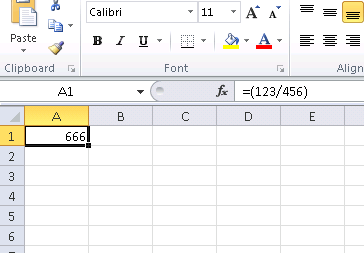
\includegraphics[scale=\NormalScale]{digging_into_code/Excel_prank.png}
\caption{\RU{Пранк сработал}\EN{The practical joke worked}}
\end{figure}

\RU{Если попробовать ту же версию Excel, только x64, то окажется что там инструкций \FDIV всего 12, 
причем нужная нам\EMDASH{}третья по счету.}
\EN{If we try the same Excel version, but in x64,
we will find only 12 \FDIV instructions there,
and the one we looking for is the third one.}

\begin{lstlisting}
tracer.exe -l:excel.exe bpx=excel.exe!BASE+0x1B7FCC,set(st0,666)
\end{lstlisting}

\index{x86!\Instructions!DIVSD}
\RU{Видимо, все дело в том, что много операций деления переменных типов \Tfloat и \Tdouble 
компилятор заменил на SSE-инструкции вроде \TT{DIVSD}, 
коих здесь теперь действительно много (\TT{DIVSD} присутствует в количестве 268 инструкций).}
\EN{It seems that a lot of division operations of \Tfloat and \Tdouble types, were replaced by the compiler with SSE instructions
like \TT{DIVSD} (\TT{DIVSD} is present 268 times in total).}

\chapter{\RU{Подозрительные паттерны кода}\EN{Suspicious code patterns}}

\section{\RU{Инструкции XOR}\EN{XOR instructions}}
\index{x86!\Instructions!XOR}

\RU{Инструкции вроде}\EN{Instructions like} \TT{XOR op, op} (\RU{например}\EN{for example}, \TT{XOR EAX, EAX}) 
\RU{обычно используются для обнуления регистра,
однако, если операнды разные, то применяется операция именно}\EN{are usually used for setting the register value
to zero, but if the operands are different, the} \q{\RU{исключающего или}\EN{exclusive or}}\EN{ operation
is executed}.
\RU{Эта операция очень редко применяется в обычном программировании, но применяется очень часто в криптографии,
включая любительскую.}
\EN{This operation is rare in common programming, but widespread in cryptography,
including amateur one.}
\RU{Особенно подозрительно, если второй операнд\EMDASH{}это большое число}\EN{It's especially suspicious if the
second operand is a big number}.
\RU{Это может указывать на шифрование, вычисление контрольной суммы,}
\EN{This may point to encrypting/decrypting, checksum computing,}\etc{}.\\
\\
\ifx\LITE\undefined
\RU{Одно из исключений из этого наблюдения о котором стоит сказать, то, что генерация и проверка значения \q{канарейки}
(\myref{subsec:BO_protection}) часто происходит, используя инструкцию \XOR.}
\EN{One exception to this observation worth noting is the \q{canary} (\myref{subsec:BO_protection}). 
Its generation and checking are often done using the \XOR instruction.} \\
\\
\fi
\index{AWK}
\RU{Этот AWK-скрипт можно использовать для обработки листингов (.lst) созданных \IDA{}}
\EN{This AWK script can be used for processing \IDA{} listing (.lst) files}:

\begin{lstlisting}
gawk -e '$2=="xor" { tmp=substr($3, 0, length($3)-1); if (tmp!=$4) if($4!="esp") if ($4!="ebp") { print $1, $2, tmp, ",", $4 } }' filename.lst
\end{lstlisting}

\ifx\LITE\undefined
\RU{Нельзя также забывать,
что если использовать подобный скрипт, то, возможно, он захватит и неверно дизассемблированный
код}\EN{It is also worth noting that this kind of script can also match incorrectly disassembled code} 
(\myref{sec:incorrectly_disasmed_code}).
\fi

\section{\RU{Вручную написанный код на ассемблере}\EN{Hand-written assembly code}}

\index{Function prologue}
\index{Function epilogue}
\index{x86!\Instructions!LOOP}
\index{x86!\Instructions!RCL}
\RU{Современные компиляторы не генерируют инструкции \TT{LOOP} и \TT{RCL}. 
С другой стороны, эти инструкции хорошо знакомы кодерам, предпочитающим писать прямо на ассемблере. 
\ifx\LITE\undefined
Подобные инструкции отмечены как (M) в списке инструкций в приложении: 
\myref{sec:x86_instructions}.
\fi
Если такие инструкции встретились, можно сказать с какой-то вероятностью, что этот фрагмент кода написан вручную.}
\EN{Modern compilers do not emit the \TT{LOOP} and \TT{RCL} instructions.
On the other hand, these instructions are well-known to coders who like to code directly in assembly language.
If you spot these, it can be said that there is a high probability that this fragment of code was hand-written.
\ifx\LITE\undefined
Such instructions are marked as (M) in the instructions list in this appendix: 
\myref{sec:x86_instructions}.
\fi
}\PTBRph{}\ESph{}\PLph{}\\
\\
\RU{Также, пролог/эпилог функции обычно не встречается в ассемблерном коде, написанном вручную.}
\EN{Also the function prologue/epilogue are not commonly present in hand-written assembly.}\\
\\
\RU{Как правило, в вручную написанном коде, нет никакого четкого метода передачи аргументов в 
функцию}
\EN{Commonly there is no fixed system for passing arguments to functions in the hand-written
code}.\\
\\
\RU{Пример из ядра}\EN{Example from the} Windows 2003\EN{ kernel} 
(\RU{файл }ntoskrnl.exe\EN{ file}):

\begin{lstlisting}
MultiplyTest proc near               ; CODE XREF: Get386Stepping
             xor     cx, cx
loc_620555:                          ; CODE XREF: MultiplyTest+E
             push    cx
             call    Multiply
             pop     cx
             jb      short locret_620563
             loop    loc_620555
             clc
locret_620563:                       ; CODE XREF: MultiplyTest+C
             retn
MultiplyTest endp

Multiply     proc near               ; CODE XREF: MultiplyTest+5
             mov     ecx, 81h
             mov     eax, 417A000h
             mul     ecx
             cmp     edx, 2
             stc
             jnz     short locret_62057F
             cmp     eax, 0FE7A000h
             stc
             jnz     short locret_62057F
             clc
locret_62057F:                       ; CODE XREF: Multiply+10
                                     ; Multiply+18
             retn
Multiply     endp
\end{lstlisting}

\RU{Действительно, если заглянуть в исходные коды}\EN{Indeed, if we look in the} 
\ac{WRK} v1.2\RU{, данный код можно найти в файле}\EN{ source code, this code
can be found easily in file} 
\IT{WRK-v1.2\textbackslash{}base\textbackslash{}ntos\textbackslash{}ke\textbackslash{}i386\textbackslash{}cpu.asm}.

\chapter{\RU{Использование magic numbers для трассировки}\EN{Using magic numbers while tracing}}

\RU{Нередко бывает нужно узнать, как используется то или иное значение, прочитанное из файла либо взятое из пакета,
принятого по сети. Часто, ручное слежение за нужной переменной это трудный процесс. Один из простых методов (хотя и не
полностью надежный на 100\%) это использование вашей собственной \IT{magic number}.}
\EN{Often, our main goal is to understand how the program uses a value that was either read from file or received via network. 
The manual tracing of a value is often a very labour-intensive task. One of the simplest techniques for this (although not 100\% reliable) 
is to use your own \IT{magic number}.}

\RU{Это чем-то напоминает компьютерную томографию: пациенту перед сканированием вводят в кровь 
рентгеноконтрастный препарат, хорошо отсвечивающий в рентгеновских лучах.
Известно, как кровь нормального человека
расходится, например, по почкам, и если в этой крови будет препарат, то при томографии будет хорошо видно,
достаточно ли хорошо кровь расходится по почкам и нет ли там камней, например, и прочих образований.}
\EN{This resembles X-ray computed tomography is some sense: a radiocontrast agent is injected into the patient's blood,
which is then used to improve the visibility of the patient's internal structure in to the X-rays.
It is well known how the blood of healthy humans
percolates in the kidneys and if the agent is in the blood, it can be easily seen on tomography, how blood is percolating,
and are there any stones or tumors.}

\RU{Мы можем взять 32-битное число вроде \TT{0x0badf00d}, либо чью-то дату рождения вроде \TT{0x11101979} 
и записать это, занимающее 4 байта число, в какое-либо место файла используемого исследуемой нами программой.}
\EN{We can take a 32-bit number like \TT{0x0badf00d}, or someone's birth date like \TT{0x11101979}
and write this 4-byte number to some point in a file used by the program we investigate.}

\index{\GrepUsage}
\index{tracer}
\RU{Затем, при трассировки этой программы, в том числе, при помощи \tracer в режиме 
\IT{code coverage}, а затем при помощи
\IT{grep} или простого поиска по текстовому файлу с результатами трассировки, мы можем легко увидеть, в каких местах кода использовалось 
это значение, и как.}
\EN{Then, while tracing this program with \tracer in \IT{code coverage} mode, with the help of \IT{grep}
or just by searching in the text file (of tracing results), we can easily see where the value was used and how.}

\RU{Пример результата работы \tracer в режиме \IT{cc}, к которому легко применить утилиту \IT{grep}}\EN{Example 
of \IT{grepable} \tracer results in \IT{cc} mode}:

\begin{lstlisting}
0x150bf66 (_kziaia+0x14), e=       1 [MOV EBX, [EBP+8]] [EBP+8]=0xf59c934 
0x150bf69 (_kziaia+0x17), e=       1 [MOV EDX, [69AEB08h]] [69AEB08h]=0 
0x150bf6f (_kziaia+0x1d), e=       1 [FS: MOV EAX, [2Ch]] 
0x150bf75 (_kziaia+0x23), e=       1 [MOV ECX, [EAX+EDX*4]] [EAX+EDX*4]=0xf1ac360 
0x150bf78 (_kziaia+0x26), e=       1 [MOV [EBP-4], ECX] ECX=0xf1ac360 
\end{lstlisting}
% TODO: good example!
\RU{Это справедливо также и для сетевых пакетов.
Важно только, чтобы наш \IT{magic number} был как можно более уникален и не присутствовал в самом коде.}
\EN{This can be used for network packets as well.
It is important for the \IT{magic number} to be unique and not to be present in the program's code.}

\newcommand{\DOSBOXURL}{\href{http://go.yurichev.com/17222}{blog.yurichev.com}}

\index{DosBox}
\index{MS-DOS}
\RU{Помимо \tracer, такой эмулятор MS-DOS как DosBox, в режиме heavydebug, может писать в отчет информацию обо всех
состояниях регистра на каждом шаге исполнения программы\footnote{См. также мой пост в блоге об этой возможности в 
DosBox: \DOSBOXURL{}}, так что этот метод может пригодиться и для исследования программ под DOS.}\EN{Aside of 
the \tracer, DosBox (MS-DOS emulator) in heavydebug mode
is able to write information about all registers' states for each executed instruction of the program to a plain text file\footnote{See also my 
blog post about this DosBox feature: \DOSBOXURL{}}, so this technique may be useful for DOS programs as well.}



\chapter{\RU{Прочее}\EN{Other things}}

\section{\EN{General idea}\RU{Общая идея}}

\RU{Нужно стараться как можно чаще ставить себя на место программиста и задавать себе вопрос, 
как бы вы сделали ту или иную вещь в этом случае и в этой программе.}
\EN{A reverse engineer should try to be in programmer's shoes as often as possible. 
To take his/her viewpoint and ask himself, how would one solve some task the specific case.}

\ifdefined\IncludeCPP
\section{\Cpp}

\ac{RTTI}~(\myref{RTTI})-\RU{информация также может быть полезна для идентификации 
классов в \Cpp}\EN{data may be also useful for \Cpp class identification}.
\fi

\section{\RU{Некоторые паттерны в бинарных файлах}\EN{Some binary file patterns}}
\index{MIPS}

\EN{Sometimes, we can clearly spot an array of 16/32/64-bit values visually, in hex editor.}
\RU{Иногда мы можем легко заметить массив 16/32/64-битных значений визуально, в шестнадцатеричном 
редакторе.}
\EN{Here is an example of very typical MIPS code.}
\RU{Вот пример очень типичного MIPS-кода.}
\EN{As we may remember, every MIPS (and also ARM in ARM mode or ARM64) instruction has size of 32 bits (or 4 bytes), 
so such code is array of 32-bit values.}
\RU{Как мы наверное помним, каждая инструкция в MIPS (а также в ARM в режиме ARM, или ARM64) имеет 
длину 32 бита (или 4 байта),
так что такой код это массив 32-битных значений.}
\EN{By looking at this screenshot, we may see some kind of pattern.}
\RU{Глядя на этот скриншот, можно увидеть некий узор.}
\EN{Vertical red lines are added for clarity}\RU{Вертикальные красные линии добавлены для ясности}:

\begin{figure}[H]
\centering
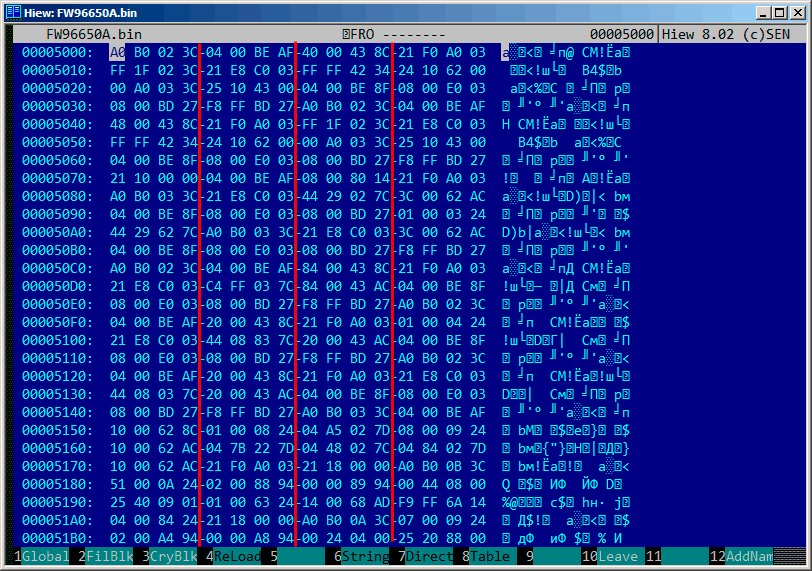
\includegraphics[scale=\NormalScale]{digging_into_code/typical_MIPS_code.png}
\caption{Hiew: \EN{very typical MIPS code}\RU{очень типичный код для MIPS}}
\end{figure}

\ifx\LITE\undefined
\RU{Еще пример таких файлов в этой книге}\EN{Another example of such pattern here is book}: 
\myref{Oracle_SYM_files_example}.
\fi

\section{\RU{Сравнение \q{снимков} памяти}\EN{Memory \q{snapshots} comparing}}
\label{snapshots_comparing}

\RU{Метод простого сравнения двух снимков памяти для поиска изменений часто применялся для взлома игр 
на 8-битных компьютерах и взлома файлов с записанными рекордными очками.}
\EN{The technique of the straightforward comparison of two memory snapshots in order to see changes was often used to hack
8-bit computer games and for hacking \q{high score} files.}

\RU{К примеру, если вы имеете загруженную игру на 8-битном компьютере (где самой памяти не очень много, но игра
занимает еще меньше), и вы знаете что сейчас у вас, условно, 100 пуль, вы можете сделать \q{снимок} всей
памяти и сохранить где-то. Затем просто стреляете куда угодно, у вас станет 99 пуль, сделать второй \q{снимок},
и затем сравнить эти два снимка: где-то наверняка должен быть байт, который в начале был 100, а затем стал 99.}
\EN{For example, if you had a loaded game on an 8-bit computer (there isn't much memory on these, but the game usually
consumes even less memory) and you know that you have now, let's say, 100 bullets, you can do a \q{snapshot}
of all memory and back it up to some place. Then shoot once, the bullet count goes to 99, do a second \q{snapshot}
and then compare both: the must be must be a byte somewhere which was 100 in the beginning, and now it is 99.}
\RU{Если учесть, что игры на тех маломощных домашних компьютерах обычно были написаны на ассемблере и подобные
переменные там были глобальные, то можно с уверенностью сказать, какой адрес в памяти всегда отвечает за количество
пуль. Если поискать в дизассемблированном коде игры все обращения по этому адресу, несложно найти код,
отвечающий за уменьшение пуль и записать туда инструкцию \gls{NOP}
или несколько \gls{NOP}-в, так мы получим игру в которой у игрока всегда будет 100 пуль, например.}
\EN{Considering the fact that these 8-bit games were often written in assembly language and such variables were global,
it can be said for sure which address in memory was holding the bullet count. If you searched for all references to the
address in the disassembled game code, it was not very hard to find a piece of code \glslink{decrement}{decrementing} the bullet count,
then to write a \gls{NOP} instruction there, or a couple of \gls{NOP}-s, 
and then have a game with 100 bullets forever.}
\index{BASIC!POKE}
\RU{А так как игры на тех домашних 8-битных 
компьютерах всегда загружались по одним и тем же адресам, и версий одной игры редко когда было больше одной продолжительное время,
то геймеры-энтузиасты знали, по какому адресу (используя инструкцию языка BASIC \gls{POKE}) что записать после загрузки
игры, чтобы хакнуть её. Это привело к появлению списков \q{читов} состоящих из инструкций \gls{POKE}, публикуемых
в журналах посвященным 8-битным играм. См. также:}\EN{Games on these 8-bit computers were commonly loaded at the constant
address, also, there were not much different versions of each game (commonly just one version was popular for a long span of time),
so enthusiastic gamers knew which bytes must be overwritten (using the BASIC's instruction \gls{POKE}) at which address in
order to hack it. This led to \q{cheat} lists that contained \gls{POKE} instructions, published in magazines related to
8-bit games. See also:} \href{http://go.yurichev.com/17114}{wikipedia}.

\index{MS-DOS}
\RU{Точно так же легко модифицировать файлы с сохраненными рекордами (кто сколько очков набрал), впрочем, это может
сработать не только с 8-битными играми. Нужно заметить, какой у вас сейчас рекорд и где-то сохранить файл
с очками. Затем, когда очков станет другое количество, просто сравнить два файла, можно даже
DOS-утилитой FC\footnote{утилита MS-DOS для сравнения двух файлов побайтово} (файлы рекордов, часто, бинарные).}
\EN{Likewise, it is easy to modify \q{high score} files, this does not work with just 8-bit games. Notice 
your score count and back up the file somewhere. When the \q{high score} count gets different, just compare the two files,
it can even be done with the DOS utility FC\footnote{MS-DOS utility for comparing binary files} (\q{high score} files
are often in binary form).}
\RU{Где-то будут отличаться несколько байт, и легко будет увидеть, какие именно отвечают за количество очков. 
Впрочем, разработчики игр полностью осведомлены о таких хитростях и могут защититься от этого.}
\EN{There will be a point where a couple of bytes are different and it is easy to see which ones are
holding the score number.
However, game developers are fully aware of such tricks and may defend the program against it.}

\ifx\LITE\undefined
\RU{В каком-то смысле похожий пример в этой книге здесь}
\EN{Somewhat similar example in this book is}: \myref{Millenium_DOS_game}.
\fi

% TODO: пример с какой-то простой игрушкой?

\subsection{\RU{Реестр Windows}\EN{Windows registry}}

\RU{А еще можно вспомнить сравнение реестра Windows до инсталляции программы и после}
\EN{It is also possible to compare the Windows registry before and after a program installation}.
\RU{Это также популярный метод поиска, какие элементы реестра программа использует.}
\EN{It is a very popular method of finding which registry elements are used by the program.}
\EN{Probably, this is the reason why the \q{windows registry cleaner} shareware is so popular.}
\RU{Наверное это причина, почему так популярны shareware-программы для очистки реестра в Windows.}

\subsection{\EN{Blink-comparator}\RU{Блинк-компаратор}}

\RU{Сравнение файлов или слепков памяти вообще, немного напоминает блинк-компаратор
\footnote{\url{http://go.yurichev.com/17349}}:
устройство, которое раньше использовали астрономы для поиска движущихся небесных объектов.}
\EN{Comparison of files or memory snapshots remind us blink-comparator
\footnote{\url{http://go.yurichev.com/17348}}:
a device used by astronomers in past, intended to find moving celestial objects.}
\RU{Блинк-компаратор позволял быстро переключаться между двух отснятых в разное время кадров,
и астроном мог увидеть разницу визуально.}
\EN{Blink-comparator allows to switch quickly between two photographies shot in different time,
so astronomer would spot the difference visually.}
\RU{Кстати, при помощи блинк-компаратора, в 1930 был открыт Плутон.}
\EN{By the way, Pluto was discovered by blink-comparator in 1930.}


\ifx\LITE\undefined
\part{\RU{Специфичное для ОС}\EN{OS-specific}}
\chapter{\RU{Способы передачи аргументов при вызове функций}\EN{Arguments passing methods (calling conventions)}}
\label{sec:callingconventions}

\section{cdecl}
\index{cdecl}
\label{cdecl}

\RU{Этот способ передачи аргументов через стек чаще всего используется в языках \CCpp.}
\EN{This is the most popular method for passing arguments to functions in the \CCpp languages.}

\RU{Вызывающая функция заталкивает в стек аргументы в обратном порядке: сначала последний аргумент в стек, 
затем предпоследний, и в самом конце\EMDASH{}первый аргумент. 
Вызывающая функция должна также затем вернуть \glslink{stack pointer}{указатель стека} в нормальное состояние, 
после возврата вызываемой функции.}
\EN{The gls{caller} also must return the value of the \gls{stack pointer} (\ESP) to its initial state after the \gls{callee} function exits.}

\begin{lstlisting}[caption=cdecl]
push arg3
push arg2
push arg1
call function
add esp, 12 ; returns ESP
\end{lstlisting}

\section{stdcall}
\label{sec:stdcall}
\index{stdcall}

\newcommand{\SIZEOFINT}{\RU{Размер переменной типа \Tint\EMDASH{}4 в x86-системах и 8 в x64-системах}
\EN{The size of an \Tint type variable is 4 in x86 systems and 8 in x64 systems}}

\RU{Это почти то же что и \IT{cdecl}, за исключением того, что вызываемая функция сама возвращает \ESP 
в нормальное состояние, выполнив инструкцию \TT{RET x} вместо \RET, где 
\TT{x = количество\_аргументов * sizeof(int)\footnote{\SIZEOFINT}}.
Вызывающая функция не будет корректировать \glslink{stack pointer}{указатель стека},
там нет инструкции \TT{add esp, x}.}
\EN{It's almost the same as \IT{cdecl}, with the exception that the \gls{callee} must set \ESP to the initial state by executing the \TT{RET x} instruction instead of \RET, where
\TT{x = arguments number * sizeof(int)\footnote{\SIZEOFINT}}.
The \gls{caller} is not adjusting the \gls{stack pointer}, 
there are no \TT{add esp, x} instruction.}

\begin{lstlisting}[caption=stdcall]
push arg3
push arg2
push arg1
call function

function:
... do something ...
ret 12
\end{lstlisting}

\RU{Этот способ используется почти везде в системных библиотеках win32, 
но не в win64 (о win64 смотрите ниже).}
\EN{The method is ubiquitous in win32 standard libraries, but not in win64 (see below about win64).}\ESph{}\PTBRph{}\PLph{} \\
\\
\RU{Например, мы можем взять функцию из}\EN{For example, we can take the function from} 
\myref{src:passing_arguments_ex} \RU{и изменить её немного добавив модификатор}\EN{and change it
slightly by adding the} \TT{\_\_stdcall}\EN{ modifier}:

\begin{lstlisting}
int __stdcall f2 (int a, int b, int c)
{
	return a*b+c;
};
\end{lstlisting}

\RU{Он будет скомпилирован почти так же как и}
\EN{It is to be compiled in almost the same way as} \myref{src:passing_arguments_ex_MSVC_cdecl},
\RU{но вы увидите}\EN{but you will see} \TT{RET 12} \RU{вместо}\EN{instead of} \TT{RET}. 
\ac{SP} \RU{не будет корректироваться в \glslink{caller}{вызывающей функции}}
\EN{is not update in the \gls{caller}}.

\RU{Как следствие, количество аргументов функции легко узнать из инструкции}\EN{As a consequence, 
the number of function arguments can be easily deduced from the} \TT{RETN n} \RU{просто разделите
$n$ на 4}\EN{instruction: just divide $n$ by 4}.

\lstinputlisting[caption=MSVC 2010]{OS/calling_conventions/stdcall_ex.asm}

\subsection{\RU{Функции с переменным количеством аргументов}\EN{Functions with variable number of arguments}}

\RU{Функции вроде \printf, должно быть, единственный случай функций в \CCpp с переменным количеством аргументов,
но с их помощью можно легко проследить очень важную разницу между \IT{cdecl} и \IT{stdcall}.
Начнем с того, что компилятор знает сколько аргументов было у \printf.}
\EN{\printf-like functions are, probably, the only case of functions with a variable number of arguments in \CCpp,
but it is easy to illustrate an important difference between \IT{cdecl} and \IT{stdcall} with their help.
Let's start with the idea that the compiler knows the argument count of each \printf function call.}
\RU{Однако, вызываемая функция \printf, которая уже давно скомпилирована 
и находится в системной библиотеке MSVCRT.DLL (если говорить о Windows), 
не знает сколько аргументов ей передали, хотя может установить их количество по строке формата.}
\EN{However, the called \printf, which is already compiled and located in MSVCRT.DLL (if we talk about Windows),
does not have any information about how much arguments were passed, however it can determine it from the format string.}
\RU{Таким образом, если бы \printf была \IT{stdcall}-функцией и возвращала
\glslink{stack pointer}{указатель стека}
в первоначальное состояние 
подсчитав количество аргументов в строке формата, это была бы потенциально опасная ситуация, 
когда одна опечатка программиста могла бы вызывать неожиданные падения программы. 
Таким образом, для таких функций \IT{stdcall} явно не подходит, а подходит \IT{cdecl}.}
\EN{Thus, if \printf would be a \IT{stdcall} function and restored \gls{stack pointer} to its initial state by counting
the number of arguments in the format string, this could be a dangerous situation, when one programmer's typo can
provoke a sudden program crash.
Thus it is not suitable for such functions to use \IT{stdcall}, \IT{cdecl} is better.}

\section{fastcall}
\label{fastcall}
\index{fastcall}

\RU{Это общее название для передачи некоторых аргументов через регистры, а всех остальных\EMDASH{}через стек.
На более старых процессорах, это работало потенциально быстрее чем \IT{cdecl}/\IT{stdcall} (ведь стек в памяти использовался меньше).
Впрочем, на современных (намного более сложных) CPU, существенного выигрыша может и не быть.}
\EN{That's the general naming for the method of passing some arguments via registers and the 
rest via the stack. It worked faster than \IT{cdecl}/\IT{stdcall} on older CPUs 
(because of smaller stack pressure).
It may not help to gain any significant performance on modern (much more complex) CPUs, however.}

\RU{Это не стандартизированный способ, поэтому разные компиляторы делают это по-своему. 
Разумеется, если у вас есть, скажем, две DLL, одна использует другую, и обе они собраны с \IT{fastcall}
но разными компиляторами, очень вероятно, будут проблемы.}
\EN{It is not standardized, so the various compilers can do it differently.
It's a well known caveat: if you have two DLLs and the one uses another one, and they are built by different compilers with 
different \IT{fastcall} calling conventions, you can expect problems.}

\RU{MSVC и GCC передает первый и второй аргумент через \ECX и \EDX а остальные аргументы через стек.}
\EN{Both MSVC and GCC pass the first and second arguments via \ECX and \EDX and the rest of the arguments via the stack.}

\RU{\glslink{stack pointer}{Указатель стека} должен быть возвращен в первоначальное состояние вызываемой функцией, 
как в случае \IT{stdcall}.}
\EN{The \gls{stack pointer} must be restored to its initial state by the \gls{callee} (like in \IT{stdcall}).}

\begin{lstlisting}[caption=fastcall]
push arg3
mov edx, arg2
mov ecx, arg1
call function

function:
.. do something ..
ret 4
\end{lstlisting}

\RU{Например, мы можем взять функцию из}\EN{For example, we may take the function from} 
\myref{src:passing_arguments_ex} \RU{и изменить её немного добавив модификатор}\EN{and change it
slightly by adding a} \TT{\_\_fastcall}\EN{ modifier}:

\begin{lstlisting}
int __fastcall f3 (int a, int b, int c)
{
	return a*b+c;
};
\end{lstlisting}

\RU{Вот как он будет скомпилирован}\EN{Here is how it is to be compiled}:

\lstinputlisting[caption=\Optimizing MSVC 2010 /Ob0]{OS/calling_conventions/fastcall_ex.asm}

\RU{Видно, что \glslink{callee}{вызываемая функция} сама возвращает}
\EN{We see that the \gls{callee} returns} \ac{SP} 
\RU{при помощи инструкции}\EN{by using the} \TT{RETN} \RU{с операндом}\EN{instruction with an operand}.
\RU{Так что и здесь можно легко вычислять количество аргументов.}
\EN{Which implies that the number of arguments can be deduced easily here as well.}

\subsection{GCC regparm}

\newcommand{\URLREGPARMM}{\url{http://go.yurichev.com/17040}}

\RU{Это в некотором роде, развитие \IT{fastcall}\footnote{\URLREGPARMM}. 
Опцией \TT{-mregparm=x} можно указывать, 
сколько аргументов компилятор будет передавать через регистры. Максимально 3. 
В этом случае будут задействованы регистры \EAX, \EDX и \ECX.}
\EN{It is the evolution of \IT{fastcall}\footnote{\URLREGPARMM} in some sense.
With the \TT{-mregparm} option it is possible to set how many arguments are to be passed via registers 
(3 is the maximum).
Thus, the \EAX, \EDX and \ECX registers are to be used.}

\RU{Разумеется, если аргументов у функции меньше трех, то будет задействована только часть регистров.}
\EN{Of course, if the number the of arguments is less than 3, not all 3 registers are to be used.}

\RU{Вызывающая функция возвращает \glslink{stack pointer}{указатель стека} в первоначальное состояние.}
\EN{The \gls{caller} restores the \gls{stack pointer} to its initial state.}

\RU{Для примера, см.}\EN{For example, see} (\myref{regparm}).

\subsection{Watcom/OpenWatcom}
\index{OpenWatcom}

\RU{Здесь это называется}\EN{Here it is called} \q{register calling convention}.
\RU{Первые 4 аргумента передаются через регистры}\EN{The first 4 arguments are passed via the}
\EAX, \EDX, \EBX \AndENRU \ECX\EN{ registers}.
\RU{Все остальные}\EN{All the rest}\EMDASH{}\RU{через стек}\EN{via the stack}.
\RU{Эти функции имеют символ подчеркивания, добавленный к концу имени функции, для отличия их от тех,
которые имеют другой способ передачи аргументов}
\EN{These functions has an underscore appended to the function name in order to distinguish them from 
those having a different calling convention}.

\section{thiscall}
\index{thiscall}

\RU{В \Cpp, это передача в функцию-метод указателя \ITthis на объект.}
\EN{This is passing the object's \ITthis pointer to the function-method, in \Cpp.}

\RU{В MSVC указатель \ITthis обычно передается в регистре \ECX.}
\EN{In MSVC, \ITthis is usually passed in the \ECX register.}

\RU{В GCC указатель \ITthis обычно передается как самый первый аргумент. 
Таким образом, внутри будет видно: у всех функций-методов на один аргумент больше.}
\EN{In GCC, the \ITthis pointer is passed as the first function-method argument.
Thus it will be very visible that internally: all function-methods have an extra argument.}

\RU{Для примера, см.}\EN{For an example, see} (\myref{thiscall}).

\section{x86-64}
\index{x86-64}

\subsection{Windows x64}
\label{sec:callingconventions_win64}

\RU{В win64 метод передачи всех параметров немного похож на \TT{fastcall}. 
Первые 4 аргумента записываются в регистры \RCX, \RDX, \Reg{8}, \Reg{9}, а остальные\EMDASH{}в стек. 
Вызывающая функция также должна подготовить место из 32 байт или для четырех 64-битных значений, 
чтобы вызываемая функция могла сохранить там первые 4 аргумента. 
Короткие функции могут использовать переменные прямо из регистров, 
но б\'{о}льшие могут сохранять их значения на будущее.}
\EN{The method of for passing arguments in Win64 somewhat resembles \TT{fastcall}.
The first 4 arguments are passed via \RCX, \RDX, \Reg{8} and \Reg{9}, the rest\EMDASH{}via the stack.
The \gls{caller} also must prepare space for 32 bytes or 4 64-bit values,
so then the \gls{callee} can save there the first 4 arguments.
Short functions may use the arguments' values just from the registers,
but larger ones may save their values for further use.}

\RU{Вызывающая функция должна вернуть \glslink{stack pointer}{указатель стека} 
в первоначальное состояние}
\EN{The \gls{caller} also must return the \gls{stack pointer} into its initial state}.

\RU{Это же соглашение используется и в системных библиотеках Windows x86-64 
(вместо \IT{stdcall} в win32).}
\EN{This calling convention is also used in Windows x86-64 system DLLs 
(instead of \IT{stdcall} in win32).}

\RU{Пример}\EN{Example}:

\lstinputlisting{OS/calling_conventions/x64.c}

\lstinputlisting[caption=MSVC 2012 /0b]{OS/calling_conventions/x64_MSVC_Ob.asm}

\index{Scratch space}
\RU{Здесь мы легко видим, как 7 аргументов передаются: 4 через регистры и остальные 3 через стек}
\EN{Here we clearly see how 7 arguments are passed: 4 via registers and the remaining 3 via the stack}.
\RU{Код пролога функции f1() сохраняет аргументы в \q{scratch space}\EMDASH{}место в стеке предназначенное
именно для этого}
\EN{The code of the f1() function's prologue saves the arguments in the \q{scratch space}\EMDASH{}a space in the stack
intended exactly for this purpose}.
\RU{Это делается потому что компилятор может быть не уверен, достаточно ли ему будет остальных регистров
для работы исключая эти 4, которые иначе будут заняты аргументами до конца исполнения функции}
\EN{This is done because the compiler can not be sure that there will be enough registers to use without these 4,
which will otherwise be occupied by the arguments until the function's execution end}.
\RU{Выделение \q{scratch space} в стеке лежит на ответственности вызывающей функции.}
\EN{The \q{scratch space} allocation in the stack is the caller's duty.}

\lstinputlisting[caption=\Optimizing MSVC 2012 /0b]{OS/calling_conventions/x64_MSVC_Ox_Ob.asm}

\RU{Если компилировать этот пример с оптимизацией, то выйдет почти то же самое, 
только \q{scratch space} не используется, потому что незачем.}
\EN{If we compile the example with optimizations, it is to be almost the same, 
but the \q{scratch space} will not be used, because it won't be needed.}

\index{x86!\Instructions!LEA}
\label{using_MOV_and_pack_of_LEA_to_load_values}
\RU{Обратите также внимание на то как MSVC 2012 оптимизирует примитивную загрузку значений в регистры
используя \LEA (\myref{sec:LEA})}
\EN{Also take a look on how MSVC 2012 optimizes the loading of primitive values into registers by using 
\LEA (\myref{sec:LEA})}.
\RU{Трудно сказать, стоит ли оно того, но может быть}\EN{It's hard to say if it worth doing so, but maybe}.

\RU{Еще один пример подобного}\EN{Another example of such thing is}: \myref{TaskMgr_LEA}.

\subsubsection{Windows x64: \RU{Передача \ITthis}\EN{Passing \ITthis} (\CCpp)}

\EN{The}\RU{Указатель} \ITthis \RU{передается через}\EN{pointer is passed in} \RCX, 
\RU{первый аргумент метода через}\EN{the first argument of the method is in} \RDX, \etc{}.
\RU{Для примера, см. также}\EN{For an example see}: \myref{simple_CPP_MSVC_x64}.
 
\subsection{Linux x64}

\RU{Метод передачи аргументов в Linux для x86-64 почти такой же, как и в Windows, но 6 регистров
используется вместо 4 (\RDI, \RSI, \RDX, \RCX, \Reg{8}, \Reg{9}), и здесь нет \q{scratch space}, 
но \gls{callee} может сохранять значения регистров в стеке, если ему это нужно.}
\EN{The way arguments are passed in Linux for x86-64 is almost the same as in Windows, but 6 registers are
used instead of 4 (\RDI, \RSI, \RDX, \RCX, \Reg{8}, \Reg{9}) and there is no \q{scratch space}, 
although the \gls{callee} may save the register values in the stack, if it needs/wants to.}

\lstinputlisting[caption=\Optimizing GCC 4.7.3]{OS/calling_conventions/x64_linux_O3.s}

\index{AMD}
\RU{N.B.: здесь значения записываются в 32-битные части регистров (например EAX) а не в весь 64-битный
регистр (RAX).
Это связано с тем что в x86-64,
запись в младшую 32-битную часть 64-битного регистра автоматически обнуляет старшие 32 бита.
Вероятно, это так решили в AMD для упрощения портирования кода под x86-64.}
\EN{N.B.: here the values are written into the 32-bit parts of the registers (e.g., EAX) but not in the whole 64-bit 
register (RAX).
This is because each write to the low 32-bit part of a register automatically clears the high 32 bits.
Supposedly, it was decided in AMD to do so to simplify porting code to x86-64.}

\section{\RU{Возвращение переменных типа \Tfloat, \Tdouble}\EN{Return values of \Tfloat and \Tdouble type}}
\index{float}
\index{double}

\RU{Во всех соглашениях кроме Win64, переменная типа \Tfloat или \Tdouble возвращается через регистр FPU \ST{0}.}
\EN{In all conventions except in Win64, the values of type \Tfloat or \Tdouble are returned via the FPU register \ST{0}.}

\RU{В Win64 переменные типа \Tfloat и \Tdouble возвращаются в младших 16-и или 32-х битах 
регистра \XMM{0}.}
\EN{In Win64, the values of \Tfloat and \Tdouble types are returned 
in the low 32 or 64 bits of the \XMM{0} register.}

\section{\RU{Модификация аргументов}\EN{Modifying arguments}}

\RU{Иногда программисты на \CCpp{} (и не только этих \ac{PL}) задаются вопросом,
что может случиться, если модифицировать аргументы?}
\EN{Sometimes, \CCpp{} programmers (not limited to these \ac{PL}s, though),
may ask, what can happen if they modify the arguments?}
\RU{Ответ прост: аргументы хранятся в стеке, именно там и будет происходит модификация.}
\EN{The answer is simple: the arguments are stored in the stack, 
that is where the modification takes place.}
\RU{А вызывающие функции не использует их после вызова функции (автор этих строк никогда не видел в своей практике обратного случая).}
\EN{The calling functions is not using them after the \gls{callee}'s exit (author of these lines have never seen any such case in his practice).}

\lstinputlisting{OS/calling_conventions/change_arguments.c}

\lstinputlisting[caption=MSVC 2012]{OS/calling_conventions/change_arguments.asm}

% TODO (OllyDbg) пример как в стеке меняется $a$

\RU{Следовательно, модифицировать аргументы функции можно запросто.}\EN{So yes, one can modify the arguments easily.}
\RU{Разумеется, если это не}\EN{Of course, if it is not} \IT{references} \InENRU \Cpp{} (\myref{cpp_references}),
\RU{и если вы не модифицируете данные по указателю}\EN{and if you not modify data to which a pointer points to}, 
\RU{то эффект не будет распространяться за пределами текущей функции}
\EN{then the effect will not propagate outside the current function}.

\RU{Теоретически, после возврата из \gls{callee},
функция-\gls{caller} могла бы получить модифицированный аргумент и использовать его как-то.
Может быть, если бы она была написана на языке ассемблера.
Но стандарты языков \CCpp не предлагают никакого способа доступиться к ним.}
\EN{Theoretically, after the \gls{callee}'s return, 
the \gls{caller} could get the modified argument and use it somehow.
Maybe if it is written directly in assembly language.
But the \CCpp languages standards don't offer any way to access them.}

% sections
\input{OS/calling_conventions/ptr_to_argument/main}

\chapter{Thread Local Storage}
\label{TLS}
\index{TLS}

\RU{Это область данных, отдельная для каждого треда. Каждый тред может хранить там то, что ему нужно}
\EN{TLS is a data area, specific to each thread. Every thread can store what it needs there}.
\RU{Один из известных примеров, это стандартная глобальная переменная в Си}%
\EN{One well-known example is the C standard global variable} \IT{errno}. 
\RU{Несколько тредов одновременно могут вызывать функции
возвращающие код ошибки в \IT{errno}, поэтому глобальная переменная здесь не будет работать корректно, 
для мультитредовых программ \IT{errno} нужно хранить в в \ac{TLS}.}
\EN{Multiple threads may simultaneously call functions
which return an error code in \IT{errno}, so a global variable will not work correctly here for multi-threaded programs,
so \IT{errno} must be stored in the \ac{TLS}.} \\
\\
\index{\Cpp!C++11}
\RU{В}\EN{In the} C++11 \RU{ввели модификатор}\EN{standard, a new} \IT{thread\_local} 
\RU{, показывающий что каждый тред будет иметь свою версию этой переменной}
\EN{modifier was added, showing that each thread has its own version of the variable},
\RU{и её можно инициализировать, и она расположена в}\EN{it can be initialized, and it is located in the} \ac{TLS}
\footnote{
\index{C11}
\RU{В C11 также есть поддержка тредов, хотя и опциональная}
\EN{C11 also has thread support, optional though}}:

\begin{lstlisting}[caption=C++11]
#include <iostream>
#include <thread>

thread_local int tmp=3;

int main()
{
	std::cout << tmp << std::endl;
};
\end{lstlisting}

\RU{Компилируется в}\EN{Compiled in} MinGW GCC 4.8.1, \RU{но не в}\EN{but not in} MSVC 2012.

\RU{Если говорить о PE-файлах, то в исполняемом файле значение}
\EN{If we talk about PE files, in the resulting executable file, the} \IT{tmp} 
\RU{будет размещено именно в секции отведенной}
\EN{variable is to be allocated in the section devoted to the} \ac{TLS}.

\section{\RU{Вернемся к линейному конгруэнтному генератору}\EN{Linear congruential generator revisited}}
\label{LCG_TLS}

\RU{Рассмотренный ранее \myref{LCG_simple} генератор псевдослучайных чисел имеет недостаток:}
\EN{The pseudorandom number generator we considered earlier \myref{LCG_simple} has a flaw:}
\RU{он не пригоден для многопоточной среды, потому что переменная его внутреннего состояния может быть
прочитана и/или модифицирована в разных потоках одновременно.}
\EN{it's not thread-safe, because it has an internal state variable which can be read and/or 
modified in different threads simultaneously.}

% subsections
\input{OS/TLS/LCG_win32}
\input{OS/TLS/LCG_linux}

\chapter{\RU{Системные вызовы (syscall-ы)}\EN{System calls (syscall-s)}}

\label{syscalls}
\index{syscall}

\index{kernel space}
\index{user space}
\RU{Как известно, все работающие процессы в \ac{OS} делятся на две категории}\EN{As we know, all running processes
inside an \ac{OS} are divided into two categories}:
\RU{имеющие полный доступ ко всему \q{железу}}\EN{those having full access to the hardware} (\q{kernel space}) 
\RU{и не имеющие}\EN{and those that do not} (\q{user space}).

\RU{В первой категории ядро \ac{OS} и, обычно, драйвера}
\EN{The \ac{OS} kernel and usually the drivers are in the first category}.

\RU{Во второй категории всё прикладное ПО}\EN{All applications are usually in the second category}.

\index{Glibc}
\EN{For example, Linux kernel is in \IT{kernel space}, but Glibc in \IT{user space}.}
\RU{Например, ядро Linux в \IT{kernel space}, но Glibc в \IT{user space}.}

\RU{Это разделение очень важно для безопасности \ac{OS}:
очень важно чтобы никакой процесс не мог испортить что-то в других процессах
или даже в самом ядре \ac{OS}}
\EN{This separation is crucial for the safety of the \ac{OS}: it is very important not to give to any process the possibility to screw up
something in other processes or even in the \ac{OS} kernel}.
\index{kernel panic}
\index{BSoD}
\RU{С другой стороны, падающий драйвер или ошибка внутри ядра \ac{OS} обычно приводит к}
\EN{On the other hand, a failing driver or error inside the \ac{OS}'s kernel usually leads to a} kernel panic \OrENRU \ac{BSOD}.

\RU{Защита x86-процессора устроена так что возможно разделить всё на 4 слоя защиты (rings), но и в Linux,
и в Windows, используются только 2}
\EN{The protection in the x86 processors allows to separate everything into 4 levels of protection (rings), but both in Linux
and in Windows only two are used}: ring0 (\q{kernel space}) \AndENRU ring3 (\q{user space}).

\RU{Системные вызовы}\EN{System calls} (syscall-\RU{ы}\EN{s})
\RU{это точка где соединяются вместе оба эти пространства}\EN{are a point where these two areas are connected}.
\RU{Это, можно сказать, самое главное \ac{API} предоставляемое прикладному ПО.}
\EN{It can be said that this is the main \ac{API} provided to applications.}

\RU{В \gls{Windows NT} таблица сисколлов находится в \ac{SSDT}}
\EN{As in \gls{Windows NT}, the syscalls table resides in the \ac{SSDT}}.

\index{Shellcode}
\RU{Работа через syscall-ы популярна у авторов шеллкодов и вирусов,
потому что там обычно бывает трудно определить адреса нужных функций в системных библиотеках,
а syscall-ами проще пользоваться, хотя и придется писать больше
кода из-за более низкого уровня абстракции этого \ac{API}}
\EN{The usage of syscalls is very popular among shellcode and computer viruses authors, 
because it is hard to determine the addresses of
needed functions in the system libraries, but it is easier to use syscalls. However, much more code has to be
written due to the lower level of abstraction of the \ac{API}}.
\RU{Также нельзя еще забывать, что номера syscall-ов могут отличаться от версии к версии OS.}
\EN{It is also worth noting that the syscall numbers may be different in various OS versions.}

\section{Linux}

\index{x86!\Instructions!INT!INT 0x80}
\RU{В Linux вызов syscall-а обычно происходит через}\EN{In Linux, a syscall is usually called via} \TT{int 0x80}.
\RU{В регистре}\EN{The call's number is passed in the} \EAX \RU{передается номер вызова,
в остальных регистрах\EMDASH{}параметры}\EN{register, and any other parameters~---in the other registers}.

\lstinputlisting[caption=\RU{Простой пример использования пары syscall-ов}\EN{A simple example of the usage of two syscalls}]
{OS/linux_syscall.s}

\RU{Компиляция}\EN{Compilation}:

\begin{lstlisting}
nasm -f elf32 1.s
ld 1.o
\end{lstlisting}

\RU{Полный список syscall-ов в}\EN{The full list of syscalls in} Linux: \url{http://go.yurichev.com/17319}.

\RU{Для перехвата и трассировки системных вызовов в Linux, можно применять}
\EN{For system calls interception and tracing in Linux,} strace(\myref{strace})\EN{ can be used}.

\section{Windows}

\index{x86!\Instructions!INT!INT 0x2e}
\index{x86!\Instructions!SYSENTER}

\RU{Вызов происходит через}\EN{Here they are called via} \TT{int 0x2e} 
\RU{либо используя специальную x86-инструкцию}\EN{or using the special x86 instruction} \TT{SYSENTER}.

\RU{Полный список syscall-ов в}\EN{The full list of syscalls in} Windows: \url{http://go.yurichev.com/17320}.

\RU{Смотрите также}\EN{Further reading}:

\q{Windows Syscall Shellcode} by Piotr Bania:\\
\url{http://go.yurichev.com/17321}.



\chapter{Linux}
\section{\CapitalPICcode}
\index{\PICcode}
\index{Linux}
\label{sec:PIC}

\RU{Во время анализа динамических библиотек (.so) в Linux, часто можно заметить такой шаблонный код}\EN{While analyzing Linux shared (.so) libraries, one may frequently spot this code pattern}:

\begin{lstlisting}[caption=libc-2.17.so x86]
.text:0012D5E3 __x86_get_pc_thunk_bx proc near         ; CODE XREF: sub_17350+3
.text:0012D5E3                                         ; sub_173CC+4 ...
.text:0012D5E3                 mov     ebx, [esp+0]
.text:0012D5E6                 retn
.text:0012D5E6 __x86_get_pc_thunk_bx endp

...

.text:000576C0 sub_576C0       proc near               ; CODE XREF: tmpfile+73

...

.text:000576C0                 push    ebp
.text:000576C1                 mov     ecx, large gs:0
.text:000576C8                 push    edi
.text:000576C9                 push    esi
.text:000576CA                 push    ebx
.text:000576CB                 call    __x86_get_pc_thunk_bx
.text:000576D0                 add     ebx, 157930h
.text:000576D6                 sub     esp, 9Ch

...

.text:000579F0                 lea     eax, (a__gen_tempname - 1AF000h)[ebx] ; "__gen_tempname"
.text:000579F6                 mov     [esp+0ACh+var_A0], eax
.text:000579FA                 lea     eax, (a__SysdepsPosix - 1AF000h)[ebx] ; "../sysdeps/posix/tempname.c"
.text:00057A00                 mov     [esp+0ACh+var_A8], eax
.text:00057A04                 lea     eax, (aInvalidKindIn_ - 1AF000h)[ebx] ; "! \"invalid KIND in __gen_tempname\""
.text:00057A0A                 mov     [esp+0ACh+var_A4], 14Ah
.text:00057A12                 mov     [esp+0ACh+var_AC], eax
.text:00057A15                 call    __assert_fail
\end{lstlisting}

\RU{Все указатели на строки корректируются при помощи некоторой константы из регистра \EBX, которая вычисляется в начале каждой функции.}
\EN{All pointers to strings are corrected by some constants and the value in \EBX,
which is calculated at the beginning of each function.}
\RU{Это так называемый адресно-независимый код (\ac{PIC}), он предназначен для исполнения будучи расположенным по любому адресу в памяти, вот почему он не содержит никаких абсолютных адресов в памяти}
\EN{This is the so-called \ac{PIC}, it is intended to be executable if placed at any random point of memory, that is why it cannot contain any absolute memory addresses}.

\RU{\ac{PIC} был очень важен в ранних компьютерных системах и важен сейчас во встраиваемых\footnote{embedded}, не имеющих поддержки виртуальной памяти (все процессы расположены в одном непрерывном блоке памяти)}
\EN{\ac{PIC} was 
crucial in early computer systems and is crucial now in embedded systems without 
virtual memory support (where all processes are placed in a single continuous memory block)}.
\RU{Он до сих пор используется в *NIX системах для динамических библиотек, потому что динамическая библиотека может использоваться одновременно в нескольких процессах, будучи загружена в память только один раз}
\EN{It is also still used in *NIX systems for shared libraries, since they 
are shared across many processes while loaded in memory only once}.
\RU{Но все эти процессы могут загрузить одну и ту же динамическую библиотеку по разным адресам, вот почему динамическая библиотека должна работать корректно, не привязываясь к абсолютным адресам}\EN{But all these processes can 
map the same shared library at different addresses, so that is why
a shared library has to work correctly without using any absolute addresses}.

\RU{Простой эксперимент}\EN{Let's do a simple experiment}:

\begin{lstlisting}
#include <stdio.h>

int global_variable=123;

int f1(int var)
{
    int rt=global_variable+var;
    printf ("returning %d\n", rt);
    return rt;
};
\end{lstlisting}

\RU{Скомпилируем в GCC 4.7.3 и посмотрим итоговый файл .so в}\EN{Let's compile it in GCC 4.7.3 and see the resulting .so file in} \IDA:

\begin{lstlisting}
gcc -fPIC -shared -O3 -o 1.so 1.c
\end{lstlisting}

\begin{lstlisting}[caption=GCC 4.7.3]
.text:00000440                 public __x86_get_pc_thunk_bx
.text:00000440 __x86_get_pc_thunk_bx proc near         ; CODE XREF: _init_proc+4
.text:00000440                                         ; deregister_tm_clones+4 ...
.text:00000440                 mov     ebx, [esp+0]
.text:00000443                 retn
.text:00000443 __x86_get_pc_thunk_bx endp

.text:00000570                 public f1
.text:00000570 f1              proc near
.text:00000570
.text:00000570 var_1C          = dword ptr -1Ch
.text:00000570 var_18          = dword ptr -18h
.text:00000570 var_14          = dword ptr -14h
.text:00000570 var_8           = dword ptr -8
.text:00000570 var_4           = dword ptr -4
.text:00000570 arg_0           = dword ptr  4
.text:00000570
.text:00000570                 sub     esp, 1Ch
.text:00000573                 mov     [esp+1Ch+var_8], ebx
.text:00000577                 call    __x86_get_pc_thunk_bx
.text:0000057C                 add     ebx, 1A84h
.text:00000582                 mov     [esp+1Ch+var_4], esi
.text:00000586                 mov     eax, ds:(global_variable_ptr - 2000h)[ebx]
.text:0000058C                 mov     esi, [eax]
.text:0000058E                 lea     eax, (aReturningD - 2000h)[ebx] ; "returning %d\n"
.text:00000594                 add     esi, [esp+1Ch+arg_0]
.text:00000598                 mov     [esp+1Ch+var_18], eax
.text:0000059C                 mov     [esp+1Ch+var_1C], 1
.text:000005A3                 mov     [esp+1Ch+var_14], esi
.text:000005A7                 call    ___printf_chk
.text:000005AC                 mov     eax, esi
.text:000005AE                 mov     ebx, [esp+1Ch+var_8]
.text:000005B2                 mov     esi, [esp+1Ch+var_4]
.text:000005B6                 add     esp, 1Ch
.text:000005B9                 retn
.text:000005B9 f1              endp
\end{lstlisting}

\newcommand{\retstring}{\IT{<<returning \%d\textbackslash{}n>>}}
\newcommand{\globvar}{\IT{global\_variable}}

\RU{Так и есть: указатели на строку \retstring{} и переменную \globvar{} корректируются при каждом исполнении функции.}%
\EN{That's it: the pointers to \retstring{} and \globvar{} are to be corrected at each function execution.}\ESph{}\PTBRph{}\PLph{}\\
\RU{Функция}\EN{The} \TT{\_\_x86\_get\_pc\_thunk\_bx()} \RU{возвращает адрес точки после вызова самой себя (здесь: \TT{0x57C}) в \EBX}\EN{function returns in \EBX the address of the point after a call to itself (\TT{0x57C} here)}.
\RU{Это очень простой способ получить значение указателя на текущую инструкцию (\EIP) в произвольном месте}
\EN{That's a simple way to get the value of the program counter (\EIP) at some point}.
\RU{Константа}\EN{The} \TT{0x1A84} \RU{связана с разницей между началом этой функции и так называемой}\EN{constant is related to the difference between this function's start and the so-called}
\IT{Global Offset Table Procedure Linkage Table} (GOT PLT), \RU{секцией, сразу же за}\EN{the section right after the} \IT{Global Offset Table} (GOT), \RU{где находится указатель на \globvar{}}\EN{where the pointer to \globvar{} is}.
\IDA \RU{показывает смещения уже обработанными, чтобы их было проще понимать, но на самом деле код такой}\EN{shows these offsets in their processed form to make them easier to understand, but in fact the code is}:

\begin{lstlisting}
.text:00000577                 call    __x86_get_pc_thunk_bx
.text:0000057C                 add     ebx, 1A84h
.text:00000582                 mov     [esp+1Ch+var_4], esi
.text:00000586                 mov     eax, [ebx-0Ch]
.text:0000058C                 mov     esi, [eax]
.text:0000058E                 lea     eax, [ebx-1A30h]
\end{lstlisting}

\RU{Так что, \EBX указывает на секцию \TT{GOT PLT} и для вычисления указателя на \globvar{}, которая хранится в \TT{GOT}, нужно вычесть 0xC}\EN{Here \EBX points to the \TT{GOT PLT} section and to calculate a pointer to \globvar{} (which is stored in 
the \TT{GOT}), \TT{0xC} must be subtracted}.
\RU{А чтобы вычислить указатель на \retstring{}, нужно вычесть \TT{0x1A30}}
\EN{To calculate pointer to the \retstring{} string, \TT{0x1A30} must be subtracted}.

\index{x86-64}
\index{x86!\Registers!RIP}
\RU{Кстати, вот зачем в AMD64 появилась поддержка адресации относительно RIP\footnote{указатель инструкций в AMD64}, просто для упрощения PIC-кода}
\EN{By the way, that is the reason why the AMD64 instruction set supports RIP\footnote{program counter in AMD64}-relative addressing\EMDASH{}to simplify PIC-code}.

\RU{Скомпилируем тот же код на Си при помощи той же версии GCC, но для x64}\EN{Let's compile the same C code using the same GCC version, but for x64}.

\index{objdump}
\RU{\IDA упростит код на выходе убирая упоминания RIP, так что будем использовать \IT{objdump} вместо нее}%
\EN{\IDA would simplify the resulting code but would suppress the RIP-relative addressing details, 
so we are going to use \IT{objdump} instead of IDA to see the everything}:

\begin{lstlisting}
0000000000000720 <f1>:
 720:	48 8b 05 b9 08 20 00 	mov    rax,QWORD PTR [rip+0x2008b9]        # 200fe0 <_DYNAMIC+0x1d0>
 727:	53                   	push   rbx
 728:	89 fb                	mov    ebx,edi
 72a:	48 8d 35 20 00 00 00 	lea    rsi,[rip+0x20]        # 751 <_fini+0x9>
 731:	bf 01 00 00 00       	mov    edi,0x1
 736:	03 18                	add    ebx,DWORD PTR [rax]
 738:	31 c0                	xor    eax,eax
 73a:	89 da                	mov    edx,ebx
 73c:	e8 df fe ff ff       	call   620 <__printf_chk@plt>
 741:	89 d8                	mov    eax,ebx
 743:	5b                   	pop    rbx
 744:	c3                   	ret    
\end{lstlisting}

\TT{0x2008b9} \RU{это разница между адресом инструкции по \TT{0x720} и \globvar{}, 
а \TT{0x20} это разница между инструкцией по \TT{0x72A} и строкой \retstring{}}
\EN{is the difference between the address of the instruction at \TT{0x720} and \globvar{}, and 
\TT{0x20} is the difference between the address of the instruction at 
\TT{0x72A} and the \retstring{} string}.

\RU{Как видно, необходимость очень часто пересчитывать адреса делает исполнение немного медленнее 
(хотя это и стало лучше в x64)}
\EN{As you might see, the need to recalculate addresses frequently makes execution slower 
(it is better in x64, though)}.
\RU{Так что если вы заботитесь о скорости исполнения, то, наверное, нужно задуматься о статической
компоновке (static linking)}
\EN{So it is probably better to link statically if you care about performance} \cite{AgnerFogCPP}.

\subsection{Windows}
\index{Windows!Win32}

\RU{Такой механизм не используется в Windows DLL. Если загрузчику в Windows приходится загружать DLL 
в другое место, он \q{патчит} DLL прямо в памяти (на местах \IT{FIXUP}-ов) чтобы скорректировать 
все адреса.}\EN{The PIC mechanism is not used in Windows DLLs. If the Windows loader needs to load DLL 
on another base address, it \q{patches} the DLL in memory (at the \IT{FIXUP} places) in order to correct 
all addresses.}
\RU{Это приводит к тому что загруженную один раз DLL нельзя использовать одновременно в разных 
	процессах, желающих расположить её по разным адресам\EMDASH{}потому что каждый загруженный в память 
экземпляр DLL \IT{доводится} до того чтобы работать только по этим адресам.}
\EN{This implies that several Windows processes cannot share an once loaded DLL 
at different addresses in different process' memory 
blocks\EMDASH{}since each instance that's loaded in memory is \IT{fixed} to work only at these addresses..}

\section{\RU{Трюк с }\IT{LD\_PRELOAD}\EN{ hack} \InENRU Linux}

\index{LD\_PRELOAD}
\label{ld_preload}

\RU{Это позволяет загружать свои динамические библиотеки перед другими, даже перед системными,
такими как}
\EN{This allows us to load our own dynamic libraries before others, even before system ones, like} libc.so.6.

\RU{Что в свою очередь, позволяет \q{подставлять} написанные нами функции перед оригинальными из системных библиотек.}
\EN{This, in turn, allows us to \q{substitute} our written functions before the original ones in the system libraries.}
\RU{Например, легко перехватывать все вызовы к}\EN{For example, it is easy to intercept all calls to} 
time(), read(), write(), \etc{}. \\
\\
\index{uptime}
\RU{Попробуем узнать, сможем ли мы обмануть утилиту \IT{uptime}}\EN{Let's see if we can fool the
\IT{uptime} utility}.
\RU{Как известно, она сообщает, как долго компьютер работает}\EN{As we know, it tells how long the computer
has been working}.
\index{strace}
\RU{При помощи}\EN{With the help of} strace(\myref{strace}), \RU{можно увидеть, что эту информацию утилита получает из файла}
\EN{it is possible to see that the utility takes this information the} \TT{/proc/uptime}
\EN{ file}:

\begin{lstlisting}
$ strace uptime 
...
open("/proc/uptime", O_RDONLY)          = 3
lseek(3, 0, SEEK_SET)                   = 0
read(3, "416166.86 414629.38\n", 2047)  = 20
...
\end{lstlisting}

\RU{Это не реальный файл на диске, это виртуальный файл,
содержимое которого генерируется на лету в ядре Linux.}
\EN{It is not a real file on disk, it is a virtual one and its contents are generated on fly in the Linux kernel.}
\RU{Там просто два числа}\EN{There are just two numbers}:

\begin{lstlisting}
$ cat /proc/uptime
416690.91 415152.03
\end{lstlisting}

\RU{Из Wikipedia, можно узнать}\EN{What we can learn from Wikipedia}
\footnote{\href{http://go.yurichev.com/17043}{wikipedia}}:

\begin{framed}
\begin{quotation}
The first number is the total number of seconds the system has been up.
The second number is how much of that time the machine has spent idle, in seconds.
\end{quotation}
\end{framed}

\index{\CStandardLibrary!open()}
\index{\CStandardLibrary!read()}
\index{\CStandardLibrary!close()}
\RU{Попробуем написать свою динамическую библиотеку, в которой будет}
\EN{Let's try to write our own dynamic library with the} open(), read(), close() 
\RU{с нужной нам функциональностью}\EN{functions working as we need}.

\RU{Во-первых, наш open() будет сравнивать имя открываемого файла с тем что нам нужно, и если да, 
то будет запоминать дескриптор открытого файла.}
\EN{At first, our open() will compare the name of the file to be opened with what we need and if it is so,
it will write down the descriptor of the file opened.}
\RU{Во-вторых, read(), если будет вызываться для этого дескриптора, будет подменять вывод,
а в остальных случаях, будет вызывать настоящий}
\EN{Second, read(), if called for this file descriptor, will substitute the output,
and in the rest of the cases will call the original} read() \RU{из}\EN{from} libc.so.6.
\RU{А также}\EN{And also} close(), \RU{будет следить, закрывается ли файл за которым мы следим.}
\EN{will note if the file we are currently following is to be closed.}

\index{dlopen()}
\index{dlsym()}
\RU{Для того чтобы найти адреса настоящих функций в libc.so.6, используем dlopen() и dlsym().}
\EN{We are going to use the dlopen() and dlsym() functions to determine the original function addresses in libc.so.6.}

\RU{Нам это нужно, потому что нам нужно передавать управление \q{настоящим} функциями.}
\EN{We need them because we must pass control to the \q{real} functions.}

\index{\CStandardLibrary!strcmp()}
\RU{С другой стороны, если бы мы перехватывали, скажем, strcmp(),
и следили бы за всеми сравнениями строк в программе, 
то, наверное, strcmp() можно было бы и самому реализовать, не
пользуясь настоящей функцией}
\EN{On the other hand, if we intercepted strcmp() and monitored each string
comparisons in the program, then we would have to implement a strcmp(), and not
use the original function}
\footnote{\RU{Например, посмотрите как обеспечивается простейший перехват strcmp()}
\EN{For example, here is how simple strcmp() interception works} \InENRU
\RU{статье}\EN{this article}
\footnote{\href{http://go.yurichev.com/17143}{yurichev.com}}
\RU{написанной}\EN{written by} Yong Huang}.

\lstinputlisting{OS/LD_PRELOAD/fool_uptime.c}
( \href{https://github.com/dennis714/RE-for-beginners/blob/master/OS/LD_PRELOAD/fool_uptime.c}{\EN{Source code at}\RU{Исходный код на} GitHub} )
% FIXME go.yurichev.com...

\RU{Компилируем как динамическую библиотеку}\EN{Let's compile it as common dynamic library}:

\begin{lstlisting}
gcc -fpic -shared -Wall -o fool_uptime.so fool_uptime.c -ldl
\end{lstlisting}

\RU{Запускаем \IT{uptime}, подгружая нашу библиотеку перед остальными}\EN{Let's run \IT{uptime}
while loading our library before the others}:

\begin{lstlisting}
LD_PRELOAD=`pwd`/fool_uptime.so uptime
\end{lstlisting}

\RU{Видим такое}\EN{And we see}:

\begin{lstlisting}
 01:23:02 up 24855 days,  3:14,  3 users,  load average: 0.00, 0.01, 0.05
\end{lstlisting}

\RU{Если переменная окружения}\EN{If the} \IT{LD\_PRELOAD} 
\RU{будет всегда указывать на путь и имя файла нашей библиотеки, то она будет
загружаться для всех запускаемых программ.}
\EN{environment variable always points to the filename and path of our library, 
it is to be loaded for all starting programs.} \\
\\
\RU{Еще примеры}\EN{More examples}:

\begin{itemize}
\RU{\item
\RU{Перехват}\EN{Intercepting} time() \InENRU Sun Solaris \href{http://go.yurichev.com/17144}{yurichev.com}
}

\item
\RU{Очень простой перехват}\EN{Very simple interception of the} strcmp() (Yong Huang) 
\url{http://go.yurichev.com/17043}

\item
Kevin Pulo\EMDASH{}Fun with LD\_PRELOAD. \RU{Много примеров и идей}\EN{A lot of examples and ideas}.
\href{http://go.yurichev.com/17145}{yurichev.com}

\item
\RU{Перехват функций работы с файлами для компрессии и декомпрессии файлов на лету}
\EN{File functions interception for compression/decompression files on fly} (zlibc). \url{http://go.yurichev.com/17146}

\end{itemize}


\chapter{Windows NT}
\section{CRT (win32)}
\label{sec:CRT}
\index{CRT}

\RU{Начинается ли исполнение программы прямо с функции \main{}}
\EN{Does the program execution start right at the \main{} function}?
\RU{Нет, не начинается}\EN{No, it does not}.
\RU{Если открыть любой исполняемый файл в \IDA или Hiew, 
то \ac{OEP} указывает на какой-то совсем другой код.}
\EN{If we would open any executable file in \IDA or HIEW, 
we can see \ac{OEP} pointing to some another code block.}
\RU{Это код, который делает некоторые приготовления перед тем как запустить ваш код}
\EN{This code is doing some maintenance and preparations before passing control flow to our code}.
\RU{Он называется стартап-код или CRT-код (C RunTime)}\EN{It is called startup-code or CRT code (C RunTime)}. \\
\\
\RU{Функция \main{} принимает на вход массив из параметров, переданных в командной строке, а также
переменные окружения}\EN{The \main{} function takes an array of the arguments passed on the command line, and also
one with environment variables}.
\RU{Но в реальности в программу передается командная строка в виде простой строки, это именно
CRT-код находит там пробелы и разрезает строку на части}\EN{But in fact a generic string is passed to the program,
the CRT code finds the spaces in it and cuts it in parts}.
\RU{CRT-код также готовит массив переменных окружения \TT{envp}}\EN{The CRT code also prepares the environment
variables array \TT{envp}}.
\RU{В \ac{GUI}-приложениях win32, вместо \main{} имеется функция \TT{WinMain} со своими аргументами}
\EN{As for \ac{GUI} win32 applications, \TT{WinMain} is used instead of \main{}, having its own arguments}:

\begin{lstlisting}
int CALLBACK WinMain(
  _In_  HINSTANCE hInstance,
  _In_  HINSTANCE hPrevInstance,
  _In_  LPSTR lpCmdLine,
  _In_  int nCmdShow
);
\end{lstlisting}

\RU{CRT-код готовит и их}\EN{The CRT code prepares them as well}.

\RU{А также, число, возвращаемое функцией \main{}, это код ошибки возвращаемый программой}
\EN{Also, the number returned by the \main{} function is the exit code}.
\RU{В CRT это значение передается в \TT{ExitProcess()}, принимающей в качестве аргумента код ошибки}
\EN{It may be passed in CRT to the \TT{ExitProcess()} function, which takes the exit code as an argument}. \\
\\
\RU{Как правило, каждый компилятор имеет свой CRT-код}\EN{Usually, each compiler has its own CRT code}. \\
\\
\RU{Вот типичный для MSVC 2008 CRT-код}\EN{Here is a typical CRT code for MSVC 2008}.

\lstinputlisting[numbers=left]{OS/win32_CRT/crt_msvc_2008.asm}

\RU{Здесь можно увидеть по крайней мере вызов
функции}\EN{Here we can see calls to} \TT{GetCommandLineA()} (\LineENRU 62), 
\RU{затем}\EN{then to} \TT{setargv()} (\LineENRU 66) \AndENRU \TT{setenvp()} (\LineENRU 74),
\RU{которые, видимо, заполняют глобальные переменные-указатели}\EN{which apparently fill the global variables}
\TT{argc}, \TT{argv}, \TT{envp}.

\RU{В итоге, вызывается \main{} с этими аргументами}\EN{Finally, \main{} is called with these arguments} 
(\LineENRU 97).

\RU{Также имеются вызовы функций с говорящими именами вроде}\EN{There are also calls to functions
with self-describing names like} \TT{heap\_init()} (\LineENRU 35), \TT{ioinit()} (\LineENRU 54).

\RU{\glslink{heap}{Куча} действительно инициализируется в \ac{CRT}}
\EN{The \glslink{heap}{heap} is indeed initialized in the \ac{CRT}}.
\RU{Если вы попытаетесь использовать}\EN{If you try to use} \TT{malloc()} 
\RU{в программе без}\EN{in a program without} CRT,
\RU{программа упадет с такой ошибкой}\EN{it will exit abnormally with the following error}:

\begin{lstlisting}
runtime error R6030
- CRT not initialized
\end{lstlisting}

\RU{Инициализация глобальных объектов в \Cpp происходит до вызова \main{}, именно в \ac{CRT}}
\EN{Global object initializations in \Cpp is also occur in the \ac{CRT} before the execution of \main{}}: 
\myref{sec:std_string_as_global_variable}.

\RU{Значение, возвращаемое из}\EN{The value that} \main{} \RU{передается или в}\EN{returns is passed to} \TT{cexit()}, 
\RU{или же в}\EN{or in} \TT{\$LN32}, \RU{которая далее вызывает}\EN{which in turn calls} \TT{doexit()}.

\RU{Можно ли обойтись без \ac{CRT}? Можно, если вы знаете что делаете.}\EN{Is it possible to get rid of the \ac{CRT}?
Yes, if you know what you are doing.}

\RU{В линкере от \ac{MSVC} точка входа задается опцией \TT{/ENTRY}}
\EN{The \ac{MSVC}'s linker has the \TT{/ENTRY} option for setting an entry point}.

\begin{lstlisting}
#include <windows.h>

int main()
{
	MessageBox (NULL, "hello, world", "caption", MB_OK);
};
\end{lstlisting}

\RU{Компилируем в}\EN{Let's compile it in} MSVC 2008.

\begin{lstlisting}
cl no_crt.c user32.lib /link /entry:main
\end{lstlisting}

\RU{Получаем вполне работающий .exe размером 2560 байт, внутри которого есть только PE-заголовок, инструкции, 
вызывающие \TT{MessageBox},
две строки в сегменте данных, импортируемая из \TT{user32.dll} функция \TT{MessageBox}, и более ничего.}
\EN{We are getting a runnable .exe with size 2560 bytes, that has a PE header in it, instructions calling
\TT{MessageBox}, two strings in the data segment,
the \TT{MessageBox} function imported from \TT{user32.dll} and nothing else.}

\RU{Это работает, но вы уже не сможете вместо \main{} написать \TT{WinMain} с его четырьмя аргументами}
\EN{This works, but you cannot write \TT{WinMain} with its 4 arguments instead of \main{}}.
\RU{Вернее, если быть точным, написать-то сможете, но доступа к этим аргументам не будет, 
потому что они не подготовлены на момент исполнения.}
\EN{To be precise, you can, but the arguments are not prepared at the moment of execution.}

\RU{Кстати, можно еще короче сделать .exe если уменьшить 
выравнивание \ac{PE}-секций (которое, по умолчанию, 4096 байт).}
\EN{By the way, it is possible to make the .exe even 
shorter by aligning the \ac{PE} sections at less than the default 4096 bytes.}

\begin{lstlisting}
cl no_crt.c user32.lib /link /entry:main /align:16
\end{lstlisting}

\RU{Линкер скажет}\EN{Linker says}:

\begin{lstlisting}
LINK : warning LNK4108: /ALIGN specified without /DRIVER; image may not run
\end{lstlisting}

\RU{Получим .exe размером 720 байт}\EN{We get an .exe that's 720 bytes}.
\RU{Он запускается в}\EN{It can be exectued in} Windows 7 x86, \RU{но не}\EN{but not in} x64 
(\RU{там выдает ошибку при загрузке}\EN{an error message will be shown when you try to execute it}).
\RU{При желании, размер можно еще сильнее ужать, но, как видно, 
возникают проблемы с совместимостью с разными версиями Windows.}
\EN{With even more efforts, it is possible
to make the executable even shorter, but as you can see, compatibility problems arise quickly.}

\section{Win32 PE}
\label{win32_pe}
\index{Windows!Win32}

\acs{PE} \RU{это формат исполняемых файлов, принятый в Windows}\EN{is an executable file format used in
Windows}.

\RU{Разница между .exe, .dll, и .sys в том, что у .exe и .sys обычно нет экспортов, только импорты}
\EN{The difference between .exe, .dll and .sys is that .exe and .sys usually do not have exports, only imports}.

\index{OEP}
\RU{У \ac{DLL}, как и у всех PE-файлов, есть точка входа (\ac{OEP})
(там располагается функция DllMain()), но обычно эта функция ничего не делает.}
\EN{A \ac{DLL}, just like any other PE-file, has an entry point (\ac{OEP}) (the function DllMain() is located there) 
but this function usually does nothing.}

.sys \RU{это обычно драйвера устройств}\EN{is usually a device driver}.

\RU{Для драйверов, Windows требует, чтобы контрольная сумма в PE-файле была проставлена
и была верной}
\EN{As of drivers, Windows requires the checksum to be present in the PE file and for it to be correct}
\footnote{\RU{Например}\EN{For example}, Hiew(\myref{Hiew}) \RU{умеет её подсчитывать}\EN{can calculate it}}.

\index{Windows!Windows Vista}
\RU{А начиная с}\EN{Starting at} Windows Vista, 
\RU{файлы драйверов должны быть также подписаны при помощи электронной подписи, 
иначе они не будут загружаться.}
\EN{a driver's files must also be signed with a digital signature. It will fail to load otherwise.}

\index{MS-DOS}
\RU{В начале всякого PE-файла есть крохотная DOS-программа,
выводящая на консоль сообщение вроде}\EN{Every PE file begins with tiny DOS program that prints a
message like} \q{This program cannot be run in DOS mode.}\EMDASH{}%
\RU{если запустить эту программу в DOS либо Windows 3.1 (\ac{OS} не знающие о PE-формате), 
выведется это сообщение.}
\EN{if you run this program in DOS or Windows 3.1 (\ac{OS}-es which are not aware of the PE format), 
this message will be printed.}

\subsection{\RU{Терминология}\EN{Terminology}}

\begin{itemize}
\item
\RU{Модуль}\EN{Module}\EMDASH{}\RU{это отдельный файл}\EN{a separate file}, .exe \OrENRU{} .dll.

\item
	\RU{Процесс}\EN{Process}\EMDASH{}\RU{это некая загруженная в память и работающая программа}\EN{a program
loaded into memory and currently running}.
\RU{Как правило состоит из одного .exe-файла и массы .dll-файлов}\EN{Commonly consists of 
one .exe file and bunch of .dll files}.

\item
	\RU{Память процесса}\EN{Process memory}\EMDASH{}\RU{память с которой работает процесс}\EN{the memory a process
works with}.
\RU{У каждого процесса\EMDASH{}своя}\EN{Each process has its own}.
\RU{Там обычно имеются загруженные модули, память стека, \glslink{heap}{кучи},}
\EN{There usually are loaded modules, memory of the stack, \gls{heap}(s),}\etc{}.

\item
\index{VA}
\ac{VA}\EMDASH{}\RU{это адрес, который будет использоваться в самой программе во время исполнения.}
\EN{an address which is to be used in program while runtime.}

\item
\index{\RU{Базовый адрес}\EN{Base address}}
\RU{Базовый адрес (модуля)}\EN{Base address (of module)}\EMDASH{}
\RU{это адрес, по которому модуль должен быть загружен в пространство процесса.}
\EN{the address within the process memory at which the module is to be loaded.}
\EN{\ac{OS} loader may change it, if the base address is already occupied by another module just loaded before.}
\RU{Загрузчик \ac{OS} может его изменить, если этот базовый адрес уже занят другим модулем, загруженным перед ним.}

\item
\index{RVA}
\ac{RVA}\EMDASH{}\RU{это}\EN{the} \ac{VA}-\RU{адрес минус базовый адрес}\EN{address minus the base address}.
\RU{Многие адреса в таблицах PE-файла используют}
\EN{Many addresses in PE-file tables use}
\ac{RVA}-\RU{адреса}\EN{addresses}.

%\item
%Data directory\EMDASH{}...

\item 
\index{Windows!IAT}
\ac{IAT}\EMDASH{}\RU{массив адресов импортированных символов}\EN{an array of addresses of imported symbols}
\footnote{\cite{Pietrek1}}. 
\RU{Иногда, директория}\EN{Sometimes, the} \TT{IMAGE\_DIRECTORY\_ENTRY\_IAT} \RU{указывает на}
\EN{data directory points at the} \ac{IAT}. 
\label{IDA_idata}
\RU{Важно отметить, что}\EN{It is worth noting that} \ac{IDA} (\RU{по крайней мере}\EN{as of} 6.1) 
\RU{может выделить псевдо-секцию с именем}\EN{may allocate a pseudo-section named} \TT{.idata} \ForENRU
\ac{IAT}, \RU{даже если}\EN{even if the} \ac{IAT} \RU{является частью совсем другой секции}
\EN{is a part of another section}!

\item 
\index{Windows!INT}
\ac{INT}\EMDASH{}\RU{массив имен символов для импортирования}
\EN{an array of names of symbols to be imported}\footnote{\cite{Pietrek1}}.
\end{itemize}

\subsection{\RU{Базовый адрес}\EN{Base address}}

\RU{Дело в том, что несколько авторов модулей могут готовить DLL-файлы для других, и нет возможности договориться о том, какие адреса и кому будут отведены.}
\EN{The problem is that several module authors can prepare DLL files for others to use and it is not possible
to reach an agreement which addresses is to be assigned to whose modules.}

\RU{Поэтому, если у двух необходимых для загрузки процесса DLL одинаковые базовые адреса,
одна из них будет загружена по этому базовому адресу, 
а вторая\EMDASH{}по другому свободному месту в памяти процесса, и все виртуальные адреса
во второй DLL будут скорректированы.}
\EN{So that is why if two necessary DLLs for a process have the same base address,
	one of them will be loaded at this base address, and the other\EMDASH{}at some other free space in process memory,
and each virtual addresses in the second DLL will be corrected.}\ESph{}\PTBRph{}\PLph{} \\
\\
\RU{Очень часто линкер в}\EN{Often,} \ac{MSVC} \RU{генерирует .exe-файлы с базовым адресом}
\EN{the linker generates the .exe files with a base address of} \TT{0x400000}
\footnote{\RU{Причина выбора такого адреса описана здесь}
\EN{The origin of this address choice is described here}: \href{http://go.yurichev.com/17041}{MSDN}},
\RU{и с секцией кода начинающейся с}\EN{and with the code section starting at} \TT{0x401000}.
\RU{Это значит, что}\EN{This mean that the} \ac{RVA} \RU{начала секции кода\EMDASH{}}\EN{of the start of the code section is} \TT{0x1000}.
\RU{А \ac{DLL} часто генерируются MSVC-линкером с базовым адресом}
\EN{DLLs are often generated by MSVC's linker with a base address of} \TT{0x10000000}
\footnote{\RU{Это можно изменять опцией /BASE в линкере}\EN{This can be changed by the /BASE linker option}}.

\index{ASLR}
\RU{Помимо всего прочего, есть еще одна причина намеренно загружать модули по разным адресам, а точнее, 
по случайным}
\EN{There is also another reason to load modules at various base addresses, in this case random ones}.

\RU{Это}\EN{It is} \ac{ASLR}\footnote{\RU{\href{http://go.yurichev.com/17042}{wikipedia}}\EN{\href{http://go.yurichev.com/17140}{wikipedia}}}.

\index{Shellcode}
\RU{Дело в том, что некий шеллкод, пытающийся исполниться на зараженной системе, должен вызывать какие-то системные функции, а следовательно, знать их адреса.}
\EN{A shellcode trying to get executed on a compromised system must call system functions, hence, know their addresses.}

\RU{И в старых}\EN{In older} \ac{OS} (\RU{в линейке \gls{Windows NT}: до}\EN{in \gls{Windows NT} line: before} Windows Vista),
\RU{системные}\EN{system} DLL (\RU{такие как}\EN{like} kernel32.dll, user32.dll) \RU{загружались все время
по одним и тем же адресам}\EN{were always loaded at known addresses}, 
\RU{а если еще и вспомнить, что версии этих DLL редко менялись}\EN{and if we also recall
that their versions rarely changed}, \RU{то адреса отдельных
функций, можно сказать, фиксированы и шеллкод может вызывать их напрямую}\EN{the addresses of functions were
fixed and shellcode could call them directly}.

\RU{Чтобы избежать этого, методика}\EN{In order to avoid this, the} \ac{ASLR}
\RU{загружает и вашу программу, и все модули ей необходимые, по случайным адресам, разным при каждом запуске}
\EN{method loads your program and all modules it needs at random base addresses, different every time}.

\RU{В PE-файлах, поддержка \ac{ASLR} отмечается выставлением флага}
\EN{\ac{ASLR} support is denoted in a PE file by setting the flag}\ESph{}\PTBRph{}\PLph{} \\
\TT{IMAGE\_DLL\_CHARACTERISTICS\_DYNAMIC\_BASE} \cite{Russinovich}.

\subsection{Subsystem}

\RU{Имеется также поле \IT{subsystem}, обычно это}\EN{There is also a \IT{subsystem} field, usually it is}:

\index{Native API}
\begin{itemize}
\item native\footnote{\EN{Meaning, the module use Native API instead of Win32}\RU{Что означает, что модуль использует Native API а не Win32}} 
(.sys-\RU{драйвер}\EN{driver}), 

\item console (\RU{консольное приложение}\EN{console application}) \OrENRU 

\item \ac{GUI} (\RU{не консольное}\EN{non-console}).
\end{itemize}

\subsection{\RU{Версия ОС}\EN{OS version}}

\RU{PE-файле также задает минимальный номер версии Windows, необходимый для загрузки модуля.}
\EN{A PE file also specifies the minimal Windows version it needs in order to be loadable.}
\RU{Соответствие номеров версий в файле и кодовых наименований Windows, можно посмотреть}
\EN{The table of version numbers stored in the PE file and corresponding Windows codenames is}
\RU{здесь}\EN{here}\footnote{\href{http://go.yurichev.com/17044}{wikipedia}}.

\index{Windows!Windows NT4}
\index{Windows!Windows 2000}
\RU{Например}\EN{For example}, \ac{MSVC} 2005 \RU{еще компилирует .exe-файлы запускающиеся на}\EN{compiles
.exe files for running on} Windows NT4 (\RU{версия}\EN{version} 4.00),
\RU{а вот}\EN{but} \ac{MSVC} 2008 \RU{уже нет}\EN{does not} 
(\RU{генерируемые файлы имеют версию}\EN{the generated files have a version of} 5.00, 
\RU{для запуска необходима как минимум Windows 2000}\EN{at least Windows 2000 is needed to run them}).

\index{Windows!Windows XP}
\RU{\ac{MSVC} 2012 по умолчанию генерирует .exe-файлы версии 6.00, для запуска нужна как минимум 
Windows Vista. 
Хотя, изменив настройки компиляции
\footnote{\href{http://go.yurichev.com/17045}{MSDN}},
можно заставить генерировать и под Windows XP.}
\EN{\ac{MSVC} 2012 generates .exe files of version 6.00 by default, 
targeting at least Windows Vista. 
However, by changing the compiler's options
\footnote{\href{http://go.yurichev.com/17045}{MSDN}},
it is possible to force it to compile for Windows XP.}

\subsection{\RU{Секции}\EN{Sections}}

\RU{Разделение на секции присутствует, по-видимому, во всех форматах исполняемых файлов.}
\EN{Division in sections, as it seems, is present in all executable file formats.}

\RU{Придумано это для того, чтобы отделить код от данных, а данные\EMDASH{}от константных данных.}
\EN{It is devised in order to separate code from data, and data\EMDASH{}from constant data.}

\begin{itemize}
\item
\RU{На секции кода будет стоять флаг}\EN{Either the} 
\IT{IMAGE\_SCN\_CNT\_CODE} \OrENRU \IT{IMAGE\_SCN\_MEM\_EXECUTE}\EN{ flags will be set on the code section}\EMDASH\RU{это исполняемый код}\EN{this is executable code}.

\item
\RU{На секции данных}\EN{On data section}\EMDASH\RU{флаги }\IT{IMAGE\_SCN\_CNT\_INITIALIZED\_DATA}, 
\IT{IMAGE\_SCN\_MEM\_READ} \AndENRU \IT{IMAGE\_SCN\_MEM\_WRITE}\EN{ flags}.

\item
\RU{На пустой секции с неинициализированными данными}\EN{On an empty section with uninitialized 
data}\EMDASH\IT{IMAGE\_SCN\_CNT\_UNINITIALIZED\_DATA}, \IT{IMAGE\_SCN\_MEM\_READ} \AndENRU \IT{IMAGE\_SCN\_MEM\_WRITE}.

\item
\RU{А на секции с константными данными, то есть, защищенными от записи}\EN{On a constant data section
(one that's protected from writing)}, \RU{могут быть флаги}
\EN{the flags} \\
\IT{IMAGE\_SCN\_CNT\_INITIALIZED\_DATA} \AndENRU \IT{IMAGE\_SCN\_MEM\_READ} \RU{без}\EN{can be set, but not} \IT{IMAGE\_SCN\_MEM\_WRITE}. 
\RU{Если попытаться записать что-то в эту секцию, процесс упадет}\EN{A process going to crash if it tries to write to this
section}.
\end{itemize}

\RU{В PE-файле можно задавать название для секции, но это не важно}\EN{Each section in PE-file may have a name, however,
it is not very important}.
\RU{Часто (но не всегда)}\EN{Often (but not always)} \RU{секция кода называется}\EN{the code section is named} \TT{.text}, 
\index{TLS}
\index{BSS}
\RU{секция данных}\EN{the data section}\EMDASH{}\TT{.data}, \RU{константных данных}\EN{the constant data section} --- \TT{.rdata} 
\IT{(readable data)}.
\RU{Еще популярные имена секций}\EN{Other popular section names are}: 

\index{MIPS}
\begin{itemize}
\item \TT{.idata}\EMDASH{}\RU{секция импортов}\EN{imports section}.
\ac{IDA} \RU{может создавать псевдо-секцию с этим же именем}
\EN{may create a pseudo-section named like this}: \myref{IDA_idata}.
\item \TT{.edata}\EMDASH{}\RU{секция экспортов (редко встречается)}\EN{exports section (rare)}
\item \TT{.pdata}\EMDASH{}\RU{секция содержащая информацию об исключениях в Windows NT для MIPS, \ac{IA64} и x64}
\EN{section containing all information about exceptions in Windows NT for MIPS, \ac{IA64} and x64}: \myref{SEH_win64}
\item \TT{.reloc}\EMDASH{}\RU{секция релоков}\EN{relocs section}
\item \TT{.bss}\EMDASH{}\RU{неинициализированные данные}\EN{uninitialized data (\ac{BSS})}
\item \TT{.tls}\EMDASH{}thread local storage (\ac{TLS})
\item \TT{.rsrc}\EMDASH{}\RU{ресурсы}\EN{resources}
\item \TT{.CRT}\EMDASH{}\RU{может присутствует в бинарных файлах, скомпилированных очень старыми версиями MSVC}
\EN{may present in binary files compiled by ancient MSVC versions}
\end{itemize}

\RU{Запаковщики/зашифровщики PE-файлов часто затирают имена секций, или меняют на свои}
\EN{PE file packers/encryptors often garble section names or replace the names with their own}.

\RU{В \ac{MSVC} можно объявлять данные в произвольно названной секции}
\EN{\ac{MSVC} allows you to declare data in arbitrarily named section}
\footnote{\href{http://go.yurichev.com/17047}{MSDN}}.

\RU{Некоторые компиляторы и линкеры могут добавлять также секцию с отладочными символами 
и вообще отладочной информацией (например, MinGW).}
\EN{Some compilers and linkers can add a section with debugging symbols and 
other debugging information (MinGW for instance).}
\index{Windows!PDB}
\RU{Хотя это не так в современных версиях}\EN{However it is not so in modern versions of} \ac{MSVC} 
(\RU{там принято отладочную информацию сохранять в отдельных \gls{PDB}-файлах}
\EN{separate \gls{PDB} files are used there for this purpose}).\\
\\
\RU{Вот как PE-секция описывается в файле}\EN{That is how a PE section is described in the file}:

\begin{lstlisting}
typedef struct _IMAGE_SECTION_HEADER {
  BYTE  Name[IMAGE_SIZEOF_SHORT_NAME];
  union {
    DWORD PhysicalAddress;
    DWORD VirtualSize;
  } Misc;
  DWORD VirtualAddress;
  DWORD SizeOfRawData;
  DWORD PointerToRawData;
  DWORD PointerToRelocations;
  DWORD PointerToLinenumbers;
  WORD  NumberOfRelocations;
  WORD  NumberOfLinenumbers;
  DWORD Characteristics;
} IMAGE_SECTION_HEADER, *PIMAGE_SECTION_HEADER;
\end{lstlisting}
\footnote{\href{http://go.yurichev.com/17048}{MSDN}}

\index{Hiew}
\RU{Еще немного терминологии}\EN{A word about terminology}:
\IT{PointerToRawData} \RU{называется}\EN{it called} \q{Offset} \InENRU Hiew
\AndENRU \IT{VirtualAddress} \RU{называется}\EN{is called} \q{RVA} \RU{там же}\EN{there}.

\subsection{\RU{Релоки}\EN{Relocations (relocs)}}
\label{subsec:relocs}

\RU{Также известны как FIXUP-ы}\EN{\ac{AKA} FIXUP-s} (\RU{по крайней мере в}\EN{at least in} Hiew).

\RU{Это также присутствует почти во всех форматах загружаемых и исполняемых файлов}
\EN{They are also present in almost all executable file formats}
\footnote{\RU{Даже .exe-файлы в}\EN{Even in .exe files for} MS-DOS}.
\EN{Exceptions are shared dynamic libraries compiled with \ac{PIC}, or any other \ac{PIC}-code.}
\RU{Исключения это динамические библиотеки явно скомпилированные с \ac{PIC} или любой другой \ac{PIC}-код.}

\RU{Зачем они нужны?}\EN{What are they for?}
\RU{Как видно, модули могут загружаться по другим базовым адресам,
но как же тогда работать с глобальными переменными, например?}
\EN{Obviously, modules can be loaded on various base addresses,
but how to deal with global variables, for example?}
\RU{Ведь нужно обращаться к ним по адресу}\EN{They must be accessed by address}.
\RU{Одно из решений\EMDASH{}это}\EN{One solution is} \PICcode{} (\myref{sec:PIC}).
\RU{Но это далеко не всегда удобно}\EN{But it is not always convenient}.

\RU{Поэтому имеется таблица релоков. 
Там просто перечислены адреса мест в модуле подлежащими коррекции при загрузке
по другому базовому адресу.}
\EN{That is why a relocations table is present.
There the addresses of points that need to be corrected are enumerated, 
in case of loading at a different base address.}

% TODO тут бы пример с HIEW или objdump..
\RU{Например, по}\EN{For example, there is a global variable at address}
\TT{0x410000} 
\RU{лежит некая глобальная переменная, и вот как обеспечивается её чтение}
\EN{and this is how it is accessed}:

\begin{lstlisting}
A1 00 00 41 00         mov         eax,[000410000]
\end{lstlisting}

\RU{Базовый адрес модуля}\EN{The base address of the module is} \TT{0x400000},
\RU{а}\EN{the} \ac{RVA} \RU{глобальной переменной}\EN{of the global variable is} \TT{0x10000}.

\RU{Если загружать модуль по базовому адресу}\EN{If the module is loaded at base address}
\TT{0x500000}, \RU{нужно чтобы адрес этой переменной в этой инструкции стал}\EN{the real address
of the global variable must be} \TT{0x510000}.

\index{x86!\Instructions!MOV}
\RU{Как видно, адрес переменной закодирован в самой инструкции}
\EN{As we can see, the address of variable is encoded in the instruction} \TT{MOV}, 
\RU{после байта}\EN{after the byte} \TT{0xA1}.

\RU{Поэтому адрес четырех байт}\EN{That is why the address of the 4 bytes}\RU{, после}\EN{ after} \TT{0xA1},
\RU{записывается в таблицу релоков}\EN{is written in the relocs table}.

\RU{Если модуль загружается по другому базовому адресу}\EN{If the module is loaded at a different base address},
\RU{загрузчик \ac{OS} обходит все адреса в таблице}\EN{the \ac{OS} loader enumerates all addresses in the table}, 
\RU{находит каждое 32-битное слово по этому адресу}
\EN{finds each 32-bit word the address points to},
\RU{отнимает от него настоящий, оригинальный базовый адрес}\EN{subtracts the original base address from it}
(\RU{в итоге получается}\EN{we get the} \ac{RVA}\EN{ here}),
\RU{и прибавляет к нему новый базовый адрес}\EN{and adds the new base address to it}.

\RU{А если модуль загружается по своему оригинальному базовому адресу, ничего не происходит}
\EN{If a module is loaded at its original base address, nothing happens}.

\RU{Так можно обходиться со всеми глобальными переменными}
\EN{All global variables can be treated like that}.

\RU{Релоки могут быть разных типов}\EN{Relocs may have various types}, 
\RU{однако в Windows для x86-процессоров, тип обычно}
\EN{however, in Windows for x86 processors, the type is usually} \\
\IT{IMAGE\_REL\_BASED\_HIGHLOW}.

\index{Hiew}
\RU{Кстати, релоки маркируются темным в Hiew, например}
\EN{By the way, relocs are darkened in Hiew, for example}: \figref{fig:scanf_ex3_hiew_1}.

\index{\olly}
\olly \RU{подчеркивает места в памяти, к которым будут применены релоки, например}\EN{underlines
the places in memory to which relocs are to be applied, for example}: \figref{fig:switch_lot_olly3}.

\subsection{\RU{Экспорты и импорты}\EN{Exports and imports}}

\label{PE_exports_imports}
\RU{Как известно}\EN{As we all know}, 
\RU{любая исполняемая программа должна как-то пользоваться сервисами \ac{OS} и прочими DLL-библиотеками}
\EN{any executable program must use the \ac{OS}'s services and other DLL-libraries somehow}.

\RU{Можно сказать, что нужно связывать функции из одного модуля (обычно DLL) и места их вызовов в 
другом модуле (.exe-файл или другая DLL)}
\EN{It can be said that functions from one module (usually DLL) must be connected somehow to the points of their
calls in other modules (.exe-file or another DLL)}.

\RU{Для этого, у каждой DLL есть \q{экспорты}, это таблица функций плюс их адреса в модуле}
\EN{For this, each DLL has an \q{exports} table, which consists of functions plus their addresses in a module}.

\RU{А у .exe-файла, либо DLL, есть \q{импорты}, это таблица функций требующихся для исполнения
включая список имен DLL-файлов}
\EN{And every .exe file or DLL has \q{imports}, a table of functions it needs for execution including
list of DLL filenames}.

\RU{Загрузчик \ac{OS}, после загрузки основного .exe-файла, проходит по таблице импортов:
загружает дополнительные DLL-файлы, 
находит имена функций среди экспортов в DLL и прописывает их адреса в \ac{IAT} в головном .exe-модуле}
\EN{After loading the main .exe-file, the \ac{OS} loader processes imports table: 
it loads the additional DLL-files, finds function names
among the DLL exports and writes their addresses down in the \ac{IAT} of the main .exe-module}.

\index{Windows!Win32!Ordinal}
\RU{Как видно, во время загрузки, загрузчику нужно много сравнивать одни имена функций с другими,
а сравнение строк\EMDASH{}это не очень быстрая процедура, так что,
имеется также поддержка \q{ординалов} или
\q{hint}-ов, это когда в таблице импортов проставлены номера функций вместо их имен}
\EN{As we can see, during loading the loader must compare a lot of function names, but string comparison is not a very
fast procedure, so there is a support for \q{ordinals} or \q{hints},
which are function numbers stored in the table, instead of their names}.

\RU{Так их быстрее находить в загружаемой DLL}
\EN{That is how they can be located faster when loading a DLL}.
\RU{В таблице экспортов ординалы присутствуют всегда}\EN{Ordinals are always present in the \q{export} table}.

\index{MFC}
\RU{К примеру}\EN{For example}, \RU{программы использующие библиотеки}\EN{a program using the} 
\ac{MFC}\RU{, обычно загружают mfc*.dll по ординалам}\EN{ library usually loads mfc*.dll by ordinals},
\RU{и в таких программах, в \ac{INT}, нет имен функций \ac{MFC}}
\EN{and in such programs there are no \ac{MFC} function names in \ac{INT}}.

% TODO example!
\RU{При загрузке такой программы в \IDA, она спросит у вас путь к файлу mfc*.dll,
чтобы установить имена функций}\EN{When loading such programs in \IDA, it will ask for a path to the mfc*.dll files
in order to determine the function names}.
\RU{Если в \IDA не указать путь к этой DLL, то вместо имен функций будет что-то вроде}
\EN{If you don't tell \IDA the path to these DLLs, there will be}
\IT{mfc80\_123}\EN{ instead of function names}.

\subsubsection{\RU{Секция импортов}\EN{Imports section}}

\RU{Под таблицу импортов и всё что с ней связано иногда отводится отдельная секция 
(с названием вроде \TT{.idata}),
но это не обязательно}
\EN{Often a separate section is allocated for the imports table and everything related to it (with name like \TT{.idata}),
however, this is not a strict rule}.

\RU{Импорты\EMDASH{}это запутанная тема еще и из-за терминологической путаницы. Попробуем собрать всё в одно место.}
\EN{Imports are also a confusing subject because of the terminological mess. Let's try to collect all information in one place.}

\begin{figure}[H]
\centering
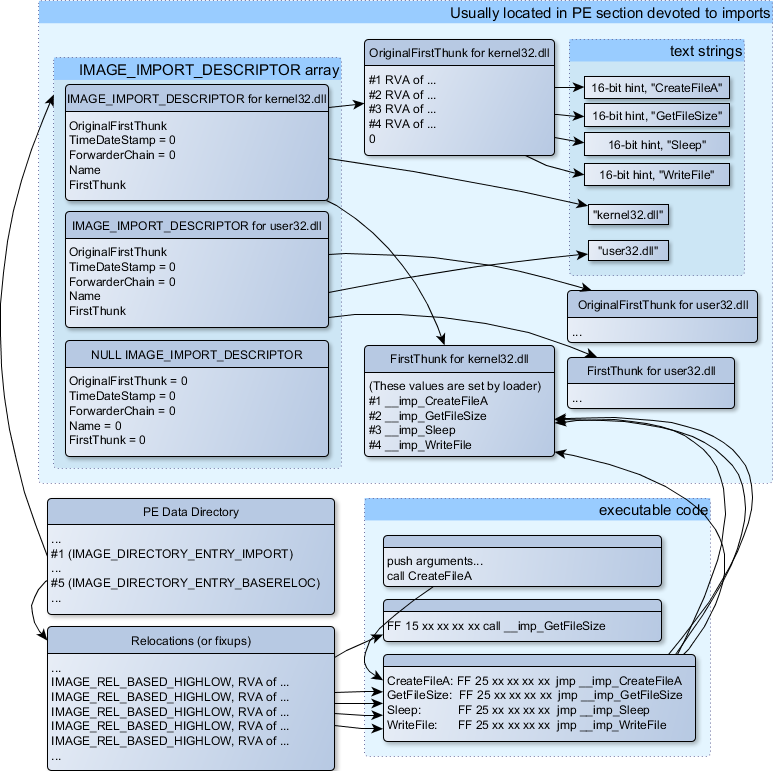
\includegraphics[scale=\FigScale]{OS/PE/unnamed0.png}
\caption{\RU{схема, объединяющая все структуры в PE-файлы, связанные с импортами}
\EN{A scheme that unites all PE-file structures related to imports}}
\end{figure}

\RU{Самая главная структура\EMDASH{}это массив}\EN{The main structure is the array} \IT{IMAGE\_IMPORT\_DESCRIPTOR}.
\RU{Каждый элемент на каждую импортируемую DLL}\EN{Each element for each DLL being imported}.

\RU{У каждого элемента есть}\EN{Each element holds the} \ac{RVA}\RU{-адрес}\EN{ address} 
\RU{текстовой строки (имя DLL)}\EN{of the text string (DLL name)} (\IT{Name}).

\IT{OriginalFirstThink} \RU{это}\EN{is the} \ac{RVA} \RU{-адрес таблицы \ac{INT}}\EN{address of the \ac{INT} table}. 
\RU{Это массив}\EN{This is an array of} 
\ac{RVA}\RU{-адресов}\EN{ addresses},
\RU{каждый из которых указывает на текстовую строку где записано имя функции}
\EN{each of which points to a text string with a function name}. 
\RU{Каждую строку предваряет 16-битное число}\EN{Each string is prefixed by a 16-bit integer} 
(\q{hint})\EMDASH\RU{\q{ординал} функции}\EN{\q{ordinal} of function}.

\RU{Если при загрузке удается найти функцию по ординалу, тогда сравнение текстовых строк не будет происходить.
Массив оканчивается нулем.}
\EN{While loading, if it is possible to find a function by ordinal,
then the strings comparison will not occur. The array is terminated by zero.}
\RU{Есть также указатель на таблицу \ac{IAT} с названием}
\EN{There is also a pointer to the \ac{IAT} table named} \IT{FirstThunk},
\RU{это просто}\EN{it is just the} \ac{RVA}\RU{-адрес}\EN{ address} 
\RU{места, где загрузчик будет проставлять адреса найденных функций}\EN{of the place where the loader
writes the addresses of the resolved functions}.

\RU{Места где загрузчик проставляет адреса, \IDA именует их так}
\EN{The points where the loader writes addresses are marked by \IDA like this}: \IT{\_\_imp\_CreateFileA}, \etc{}.

\RU{Есть по крайней мере два способа использовать адреса, проставленные загрузчиком}
\EN{There are at least two ways to use the addresses written by the loader}.

\begin{itemize}
\index{x86!\Instructions!CALL}
\item
\RU{В коде будут просто инструкции вроде}\EN{The code will have instructions like} 
\IT{call \_\_imp\_CreateFileA}, 
\RU{а так как, поле с адресом импортируемой функции это как бы глобальная переменная}
\EN{and since the field with the address of the imported function is a global variable in some sense}, 
\RU{то в таблице релоков добавляется адрес (плюс 1 или 2) в инструкции \IT{call}}
\EN{the address of the \IT{call} instruction (plus 1 or 2) is to be added to the relocs table},
\RU{на случай если модуль будет загружен по другому базовому адресу}
\EN{for the case when the module is loaded at a different base address}.

\RU{Но как видно, это приводит к увеличению таблицы релоков}\EN{But, obviously, this may enlarge
relocs table significantly}.
\RU{Ведь вызовов импортируемой функции у вас в модуле может быть очень много}
\EN{Because there are might be a lot of calls to imported functions in the module}.
\RU{К тому же, чем больше таблица релоков, тем дольше загрузка}
\EN{Furthermore, large relocs table slows down the process of loading modules}.

\index{x86!\Instructions!JMP}
\index{thunk-\RU{функции}\EN{functions}}
\item
\RU{На каждую импортируемую функцию выделяется только один переход на импортируемую функцию используя
инструкцию \JMP плюс релок на эту инструкцию}
\EN{For each imported function, there is only one jump allocated, using the \JMP instruction 
plus a reloc to it}.
\RU{Такие места-\q{переходники} называются также \q{thunk}-ами}\EN{Such points are also called \q{thunks}}.
\RU{А все вызовы импортируемой функции это просто инструкция \CALL на соответствующий \q{thunk}}
\EN{All calls to the imported functions are just \CALL instructions to the corresponding \q{thunk}}.
\RU{В данном случае, дополнительные релоки не нужны, потому что эти CALL-ы имеют относительный адрес,
и корректировать их не надо}\EN{In this case, additional relocs are not necessary because these CALL-s
have relative addresses and do not need to be corrected}.
\end{itemize}

\RU{Оба этих два метода могут комбинироваться}\EN{These two methods can be combined}.
\RU{Вероятно, линкер создает отдельный \q{thunk}, если вызовов слишком много, но по умолчанию\EMDASH{}не создает.}
\EN{Possible, the linker creates individual \q{thunk}s if there are too many calls to the function,
but not done by default.} \\
\\
\RU{Кстати, массив адресов функций, на который указывает FirstThunk,
не обязательно может быть в секции \ac{IAT}}\EN{By the way, the array of function addresses to which FirstThunk is
pointing is not necessary to be located in the \ac{IAT} section}.
\RU{К примеру, автор сих строк написал утилиту}\EN{For example, author of these lines once wrote the}
PE\_add\_import\footnote{\href{http://go.yurichev.com/17049}{yurichev.com}} 
\RU{для добавления импорта в уже существующий .exe-файл}\EN{utility for adding imports to an existing .exe-file}.
\RU{Раньше, в прошлых версиях утилиты, на месте функции, вместо которой вы хотите подставить вызов в другую DLL,
моя утилита вписывала такой код:}
\EN{Some time earlier, in the previous versions of the utility, 
at the place of the function you want to substitute with a call to another DLL,
my utility wrote the following code:}

\begin{lstlisting}
MOV EAX, [yourdll.dll!function]
JMP EAX
\end{lstlisting}

\RU{При этом, FirstThunk указывает прямо на первую инструкцию.
Иными словами, загрузчик, загружая yourdll.dll, 
прописывает адрес функции \IT{function} прямо в коде.}
\EN{FirstThunk points to the first instruction. In other words, when loading yourdll.dll,
the loader writes the address of the \IT{function} function right in the code.}

\RU{Надо также отметить что обычно секция кода защищена от записи}
\EN{It also worth noting that a
code section is usually write-protected}, \RU{так что, моя утилита
добавляет флаг}\EN{so my utility adds the} \\
\IT{IMAGE\_SCN\_MEM\_WRITE} 
\RU{для секции кода. Иначе при загрузке такой программы, она упадет с ошибкой}
\EN{flag for code section. Otherwise, the program to crash while loading with error code}
5 (access denied). \\
\\
\RU{Может возникнуть вопрос: а что если я поставляю программу с набором DLL,
которые никогда не будут меняться (в т.ч., адреса всех функций в этих DLL), может как-то можно ускорить процесс загрузки?}
\EN{One might ask: what if I supply a program with a set of DLL files which is not supposed to change (including addresses of all DLL functions),
is it possible to speed up the loading process?}

\RU{Да, можно прописать адреса импортируемых функций в массивы FirstThunk заранее}
\EN{Yes, it is possible to write the addresses of the functions to be imported into the FirstThunk arrays in advance}.
\RU{Для этого в структуре}\EN{The \IT{Timestamp} field is present in the} \\
\IT{IMAGE\_IMPORT\_DESCRIPTOR} \RU{имеется поле \IT{Timestamp}}\EN{structure}.
\RU{И если там присутствует какое-то значение, то загрузчик сверяет это значение с датой-временем DLL-файла}
\EN{If a value is present there, then the loader compares this value with the date-time of the DLL file}.
\RU{И если они равны, то загрузчик больше ничего не делает, и загрузка может происходить быстрее.}
\EN{If the values are equal, then the loader does not do anything, and the loading of the process can be faster.}
\RU{Это называется}\EN{This is called} \q{old-style binding}
\footnote{\href{http://go.yurichev.com/17050}{MSDN}.
\RU{Существует также}\EN{There is also the} \q{new-style binding}.}.
\index{BIND.EXE}
\RU{В Windows SDK для этого имеется утилита BIND.EXE}
\EN{The BIND.EXE utility in Windows SDK is for for this}.
\RU{Для ускорения загрузки вашей программы}\EN{For speeding up the loading of your program}, 
Matt Pietrek \InENRU \cite{Pietrek1}, \RU{предлагает делать binding сразу после инсталляции
вашей программы на компьютере конечного пользователя}\EN{suggests to do the binding shortly after your program
installation on the computer of the end user}. \\
\\
\RU{Запаковщики/зашифровщики PE-файлов могут также сжимать/шифровать таблицу импортов}
\EN{PE-files packers/encryptors may also compress/encrypt imports table}.
\RU{В этом случае, загрузчик Windows, конечно же, не загрузит все нужные DLL}
\EN{In this case, the Windows loader, of course, will not load all necessary DLLs}.
\index{Windows!Win32!LoadLibrary}
\index{Windows!Win32!GetProcAddress}
\RU{Поэтому распаковщик/расшифровщик делает это сам, при помощи вызовов}
\EN{Therefore, the packer/encryptor does this on its own, with the help of} 
\IT{LoadLibrary()} \AndENRU \EN{the }\IT{GetProcAddress()}\EN{ functions}.
\RU{Вот почему в запакованных файлах эти две функции часто присутствуют в \ac{IAT}.}
\EN{That is why these two functions are often present in \ac{IAT} in packed files.}\\
\\
\RU{В стандартных DLL входящих в состав Windows, часто, \ac{IAT} находится в самом начале PE-файла.}
\EN{In the standard DLLs from the Windows installation, \ac{IAT} often is located right in the beginning of the PE file.}
\RU{Возможно это для оптимизации}\EN{Supposedly, it is done for optimization}.
\RU{Ведь .exe-файл при загрузке не загружается в память весь 
(вспомните что инсталляторы огромного размера подозрительно быстро запускаются), он \q{мапится} (map), 
и подгружается в память частями по мере обращения к этой памяти.}
\EN{While loading, the .exe file is not loaded into memory as a whole (recall huge install programs which are
started suspiciously fast), it is \q{mapped}, and loaded into memory in parts as they are accessed.}
\RU{И возможно в Microsoft решили что так будет быстрее.}
\EN{Probably, Microsoft developers decided it will be faster.}

\subsection{\RU{Ресурсы}\EN{Resources}}

\label{PEresources}
\RU{Ресурсы в PE-файле\EMDASH{}это набор иконок, картинок, текстовых строк, описаний диалогов}
\EN{Resources in a PE file are just a set of icons, pictures, text strings, dialog descriptions}.
\RU{Возможно, их в свое время решили отделить от основного кода, чтобы все эти вещи были многоязычными,
и было проще выбирать текст или картинку того языка, который установлен в \ac{OS}}
\EN{Perhaps, they were separated from the main code, so all these things could be multilingual,
and it would be simpler to pick text or picture for the language that is currently set in the \ac{OS}}. \\
\\
\RU{В качестве побочного эффекта, их легко редактировать и сохранять обратно в исполняемый файл,
даже не обладая специальными знаниями, например, редактором ResHack}%
\EN{As a side effect, they can be edited easily and saved back to the executable file, even if one does not have special knowledge, 
by using the ResHack editor, for example} (\myref{ResHack}).

\subsection{.NET}

\index{.NET}
\RU{Программы на .NET компилируются не в машинный код, а в свой собственный байткод}
\EN{.NET programs are not compiled into machine code but into a special bytecode}.
\index{OEP}
\RU{Собственно, в .exe-файлы байткод вместо обычного кода, однако, точка входа (\ac{OEP}) 
указывает на крохотный фрагмент x86-кода}\EN{Strictly speaking, there is bytecode instead of the usual x86 code
in the .exe file, however, the entry point (\ac{OEP}) points to this tiny fragment of x86 code}:

\begin{lstlisting}
jmp         mscoree.dll!_CorExeMain
\end{lstlisting}

\RU{А в mscoree.dll и находится .NET-загрузчик, который уже сам будет работать с PE-файлом.}
\EN{The .NET loader is located in mscoree.dll, which processes the PE file.}
\index{Windows!Windows XP}
\RU{Так было в \ac{OS} до Windows XP. Начиная с XP, загрузчик \ac{OS} уже сам определяет, что это
.NET-файл и запускает его не исполняя этой инструкции \JMP}
\EN{It was so in all pre-Windows XP \ac{OS}es. Starting from XP, the \ac{OS} loader is able to detect the .NET file
and run it without executing that \JMP instruction}
\footnote{\href{http://go.yurichev.com/17051}{MSDN}}.

\index{TLS}
\subsection{TLS}

\RU{Эта секция содержит в себе инициализированные данные для}\EN{This section holds initialized
data for the} \ac{TLS}(\myref{TLS}) (\RU{если нужно}\EN{if needed}).
\RU{При старте нового треда, его}\EN{When a new thread start, its} 
\ac{TLS}\RU{-данные инициализируются данными из этой секции}
\EN{data is initialized using the data from this section}. \\
\\
\index{TLS!Callbacks}
\RU{Помимо всего прочего, спецификация PE-файла предусматривает инициализацию}
\EN{Aside from that, the PE file specification also provides initialization of the}
\ac{TLS}\RU{-секции, т.н.,}\EN{ section, the so-called} TLS callbacks.
\RU{Если они присутствуют, то они будут вызваны перед тем как передать управление на главную точку входа}
\EN{If they are present, they are to be called before the control is passed to the main entry point} (\ac{OEP}).
\RU{Это широко используется запаковщиками/защифровщиками PE-файлов.}
\EN{This is used widely in the PE file packers/encryptors.}

\subsection{\RU{Инструменты}\EN{Tools}}

\begin{itemize}
\item
\index{objdump}
\index{Cygwin}
objdump (\RU{имеется в}\EN{present in} cygwin) \RU{для вывода всех структур PE-файла}\EN{for dumping all PE-file structures}.

\item
\index{Hiew}
Hiew(\myref{Hiew}) \RU{как редактор}\EN{as editor}.

\item
	pefile\EMDASH{}Python-\RU{библиотека для работы с PE-файлами}\EN{library for PE-file processing}
\footnote{\url{http://go.yurichev.com/17052}}.

\item
\label{ResHack}
ResHack \acs{AKA} Resource Hacker\EMDASH{}\RU{редактор ресурсов}\EN{resources editor}
\footnote{\url{http://go.yurichev.com/17052}}.

\item
	PE\_add\_import\footnote{\url{http://go.yurichev.com/17049}}\EMDASH{}
\RU{простая утилита для добавления символа/-ов в таблицу импортов PE-файла}
\EN{simple tool for adding symbol(s) to PE executable import table}.

\item
	PE\_patcher\footnote{\href{http://go.yurichev.com/17054}{yurichev.com}}\EMDASH{} 
\RU{простая утилита для модификации PE-файлов}\EN{simple tool for patching PE executables}.

\item
	PE\_search\_str\_refs\footnote{\href{http://go.yurichev.com/17055}{yurichev.com}}\EMDASH{} 
\RU{простая утилита для поиска функции в PE-файле, где используется некая текстовая строка}
\EN{simple tool for searching for a function in PE executables which use some text string}.
\end{itemize}

\subsection{Further reading}

% FIXME: bibliography per chapter or section
\begin{itemize}
\item
Daniel Pistelli\EMDASH{}The .NET File Format \footnote{\url{http://go.yurichev.com/17056}}
\end{itemize}


\section{Windows SEH}
\label{sec:SEH}
\index{Windows!Structured Exception Handling}

\newcommand{\HandlerFunction}{\RU{функция-обработчик}\EN{handler function}}
\newcommand{\MoreEntries}{\RU{остальные элементы}\EN{more entries}}
\newcommand{\FilterFunction}{\RU{функция-фильтр}\EN{filter function}}
\newcommand{\HandlerFinallyFunction}{\RU{функция-обработчик/finally-обработчик}\EN{handler/finally function}}
\newcommand{\ScopeTable}{\RU{таблица scope}\EN{scope table}}

% subsections
\input{OS/SEH/1/main}
\input{OS/SEH/2/main}
\input{OS/SEH/3/main}

\subsection{\RU{Больше о}\EN{Read more about} SEH}

\cite{PietrekSEH}, \cite{IgorSkochinsky}.

\section{Windows NT: \RU{Критические секции}\EN{Critical section}}
\index{Windows}

\label{critical_sections}

\RU{Критические секции в любой \ac{OS} очень важны в мультитредовой среде, используются в основном
для обеспечения гарантии что только один тред будет иметь доступ к данным в один момент времени,
блокируя остальные треды и прерывания.}
\EN{Critical sections in any \ac{OS} are very important in multithreaded environment,
mostly for giving a guarantee
that only one thread can access some data in a single moment of time, 
while blocking other threads and interrupts.}\ESph{}\PTBRph{}\PLph{} \\
\\
\RU{Вот как объявлена структура}\EN{That is how a} \TT{CRITICAL\_SECTION} 
\RU{объявлена в линейке OS}\EN{structure is declared in} \gls{Windows NT}\EN{ line OS}:

\begin{lstlisting}[caption=(Windows Research Kernel v1.2) public/sdk/inc/nturtl.h]
typedef struct _RTL_CRITICAL_SECTION {
    PRTL_CRITICAL_SECTION_DEBUG DebugInfo;

    //
    //  The following three fields control entering and exiting the critical
    //  section for the resource
    //

    LONG LockCount;
    LONG RecursionCount;
    HANDLE OwningThread;        // from the thread's ClientId->UniqueThread
    HANDLE LockSemaphore;
    ULONG_PTR SpinCount;        // force size on 64-bit systems when packed
} RTL_CRITICAL_SECTION, *PRTL_CRITICAL_SECTION;
\end{lstlisting}

\RU{Вот как работает функция}\EN{That's is how} EnterCriticalSection()\EN{ function works}:

\index{x86!\Instructions!LOCK}
\begin{lstlisting}[caption=Windows 2008/ntdll.dll/x86 (begin)]
_RtlEnterCriticalSection@4

var_C           = dword ptr -0Ch
var_8           = dword ptr -8
var_4           = dword ptr -4
arg_0           = dword ptr  8

                mov     edi, edi
                push    ebp
                mov     ebp, esp
                sub     esp, 0Ch
                push    esi
                push    edi
                mov     edi, [ebp+arg_0]
                lea     esi, [edi+4] ; LockCount
                mov     eax, esi
                lock btr dword ptr [eax], 0
                jnb     wait ; jump if CF=0

loc_7DE922DD:
                mov     eax, large fs:18h
                mov     ecx, [eax+24h]
                mov     [edi+0Ch], ecx
                mov     dword ptr [edi+8], 1
                pop     edi
                xor     eax, eax
                pop     esi
                mov     esp, ebp
                pop     ebp
                retn    4

... skipped
\end{lstlisting}

\index{x86!\Instructions!BTR}
\index{x86!\Prefixes!LOCK}
\RU{Самая важная инструкция в этом фрагменте кода\EMDASH{}это}
\EN{The most important instruction in this code fragment is} \TT{BTR} 
(\RU{с префиксом}\EN{prefixed with} \TT{LOCK}): 
\RU{нулевой бит сохраняется в флаге CF и очищается в памяти}
\EN{the zeroth bit is stored in the CF flag and cleared in memory}.
\RU{Это \glslink{atomic operation}{атомарная операция}}\EN{This is an \gls{atomic operation}}, 
\RU{блокирующая доступ всех остальных процессоров
к этому значению в памяти (обратите внимание на префикс \TT{LOCK} перед инструкцией \TT{BTR}.}
\EN{blocking all other CPUs' access to this piece of memory 
(see the \TT{LOCK} prefix before the \TT{BTR} instruction).}
\RU{Если бит в}\EN{If the bit at} \TT{LockCount} \RU{является}\EN{is} 1, 
\RU{хорошо, сбросить его и вернуться из функции: мы в критической секции}
\EN{fine, reset it and return from the function: we are in a critical section}.
\RU{Если нет\EMDASH{}критическая секция уже занята другим тредом, тогда ждем}
\EN{If not\EMDASH{}the critical section is already occupied by other thread, so wait}. \\
\RU{Ожидание там сделано через вызов}\EN{The wait is done there using} WaitForSingleObject(). \\
\\
\RU{А вот как работает функция}\EN{And here is how the} LeaveCriticalSection()\EN{ function works}:

\begin{lstlisting}[caption=Windows 2008/ntdll.dll/x86 (begin)]
_RtlLeaveCriticalSection@4 proc near

arg_0           = dword ptr  8

                mov     edi, edi
                push    ebp
                mov     ebp, esp
                push    esi
                mov     esi, [ebp+arg_0]
                add     dword ptr [esi+8], 0FFFFFFFFh ; RecursionCount
                jnz     short loc_7DE922B2
                push    ebx
                push    edi
                lea     edi, [esi+4]    ; LockCount
                mov     dword ptr [esi+0Ch], 0
                mov     ebx, 1
                mov     eax, edi
                lock xadd [eax], ebx
                inc     ebx
                cmp     ebx, 0FFFFFFFFh
                jnz     loc_7DEA8EB7

loc_7DE922B0:
                pop     edi
                pop     ebx

loc_7DE922B2:
                xor     eax, eax
                pop     esi
                pop     ebp
                retn    4

... skipped
\end{lstlisting}

\index{x86!\Instructions!XADD}
\TT{XADD} \RU{это \q{обменять и прибавить}}\EN{is \q{exchange and add}}.
\RU{В данном случае, это значит прибавить 1 к значению в \TT{LockCount}, сохранить результат
в регистре \TT{EBX}, и в то же время 1 записывается в \TT{LockCount}}
\EN{In this case, it adds 1 to \TT{LockCount} and stores the result in the \TT{EBX} register, 
and at the same time 1 goes to \TT{LockCount}}.
\RU{Эта операция также атомарная, потому что также имеет префикс \TT{LOCK}, что означает, что другие CPU
или ядра CPU в системе не будут иметь доступа к этой ячейке памяти}
\EN{This operation is atomic since it is prefixed by \TT{LOCK} as well,
meaning that all other CPUs or CPU cores in system are blocked from accessing this point in memory}.

\EN{The}\RU{Префикс} \TT{LOCK} \RU{очень важен}\EN{prefix is very important}: 
\RU{два треда, каждый из которых работает на разных CPU или ядрах CPU, могут попытаться одновременно
войти в критическую секцию, одновременно модифицируя значение в памяти, и это может привести к
непредсказуемым результатам.}
\EN{without it two threads, each of which works on separate CPU or CPU core can try to
enter a critical section and to modify the value in memory,
which will result in non-deterministic behaviour.}

% TODO linux



\fi
\part{\RU{Инструменты}\EN{Tools}}

\chapter{\RU{Дизассемблер}\EN{Disassembler}}

\section{IDA}

\label{IDA}
\RU{Старая бесплатная версия доступна для скачивания}\EN{An older freeware version is available for download}
\footnote{\href{http://go.yurichev.com/17031}{hex-rays.com/products/ida/support/download\_freeware.shtml}}.

\ifx\LITE\undefined
\ShortHotKeyCheatsheet: \myref{sec:IDA_cheatsheet}
\fi

\chapter{\RU{Отладчик}\EN{Debugger}}

\ifdefined\IncludeOlly
\section{\olly}
\index{\olly}

\RU{Очень популярный отладчик пользовательской среды win32}\EN{Very popular user-mode win32 debugger}:\\
\href{http://go.yurichev.com/17032}{ollydbg.de}.

\ShortHotKeyCheatsheet: \myref{sec:Olly_cheatsheet}
\fi

\ifdefined\IncludeGDB
\section{GDB}
\index{GDB}

\RU{Не очень популярный отладчик у реверсеров, тем не менее, крайне удобный}\EN{Not very popular
debugger among reverse engineers, but very comfortable nevertheless}.
\RU{Некоторые команды}\EN{Some commands}: \myref{sec:GDB_cheatsheet}.
\fi

\section{tracer}

\index{tracer}
\label{tracer}
\RU{Автор часто использует}\EN{The author often use} \IT{tracer}\footnote{\EN{\href{http://go.yurichev.com/17338}{yurichev.com}}\RU{\href{http://go.yurichev.com/17339}{yurichev.com}}}
\RU{вместо отладчика}\EN{instead of a debugger}.

\RU{Со временем, автор этих строк отказался использовать отладчик, потому что всё что ему нужно от него это иногда подсмотреть 
какие-либо аргументы какой-либо функции во время исполнения или состояние регистров в определенном месте. 
Каждый раз загружать отладчик для этого это слишком, поэтому родилась очень простая утилита \IT{tracer}. 
Она консольная, запускается из командной строки, позволяет перехватывать исполнение функций, 
ставить точки останова на произвольные места, смотреть состояние регистров, модифицировать их, \etc.}
\EN{The author of these lines stopped using a debugger eventually, since all he need from it is to spot function arguments while
executing, or registers state at some point.
Loading a debugger each time is too much, so a small utility called \IT{tracer} was born.
It works from command line, allows intercepting function execution,
setting breakpoints at arbitrary places, reading and changing registers state, etc.}

\RU{Но для учебы очень полезно трассировать код руками в отладчике, наблюдать как меняются значения регистров 
(например, как минимум классический SoftICE, OllyDbg, WinDbg подсвечивают измененные регистры), 
флагов, данные, менять их самому, смотреть реакцию, \etc.}
\EN{However, for learning purposes it is highly advisable to trace code in a debugger manually, watch how the registers state
changes (e.g. classic SoftICE, OllyDbg, WinDbg highlight changed registers), flags, data, change them
manually, watch the reaction, \etc{}.}

\ifx\LITE\undefined
\chapter{\RU{Трассировка системных вызовов}\EN{System calls tracing}}

\label{strace}
\index{strace}
\index{dtruss}
\subsection{strace / dtruss}

\index{syscall}
\RU{Позволяет показать, какие системные вызовы (syscalls(\myref{syscalls})) прямо сейчас вызывает процесс.}
\EN{It shows which system calls (syscalls(\myref{syscalls})) are called by a process right now.}
\RU{Например}\EN{For example}:

\begin{lstlisting}
# strace df -h

...

access("/etc/ld.so.nohwcap", F_OK)      = -1 ENOENT (No such file or directory)
open("/lib/i386-linux-gnu/libc.so.6", O_RDONLY|O_CLOEXEC) = 3
read(3, "\177ELF\1\1\1\0\0\0\0\0\0\0\0\0\3\0\3\0\1\0\0\0\220\232\1\0004\0\0\0"..., 512) = 512
fstat64(3, {st_mode=S_IFREG|0755, st_size=1770984, ...}) = 0
mmap2(NULL, 1780508, PROT_READ|PROT_EXEC, MAP_PRIVATE|MAP_DENYWRITE, 3, 0) = 0xb75b3000
\end{lstlisting}

\index{\MacOSX}
\RU{В \MacOSX для этого же имеется dtruss}\EN{\MacOSX has dtruss for doing the same}.

\index{Cygwin}
\RU{В Cygwin также есть strace, впрочем, насколько известно, 
он показывает результаты только для .exe-файлов скомпилированных для среды самого cygwin.}%
\EN{Cygwin also has strace, but as far as it's known, it works only for .exe-files
compiled for the cygwin environment itself.}
\fi

\chapter{\RU{Декомпиляторы}\EN{Decompilers}}

\RU{Пока существует только один публично доступный декомпилятор в Си высокого качества}
\EN{There is only one known, publicly available, high-quality decompiler to C code}: Hex-Rays:\\
\href{http://go.yurichev.com/17033}{hex-rays.com/products/decompiler/}

% TODO Java, .NET, VB, etc

\chapter{\RU{Прочие инструменты}\EN{Other tools}}

\begin{itemize}
\item
Microsoft Visual Studio Express\footnote{\href{http://go.yurichev.com/17034}{visualstudio.com/en-US/products/visual-studio-express-vs}}:
\RU{Усеченная бесплатная версия Visual Studio, пригодная для простых экспериментов.}
\EN{Stripped-down free version of Visual Studio, convenient for simple experiments.}
\ifx\LITE\undefined
\RU{Некоторые полезные опции}\EN{Some useful options}: \myref{sec:MSVC_options}.
\fi

\item
\label{Hiew}
Hiew\footnote{\href{http://go.yurichev.com/17035}{hiew.ru}} \RU{для мелкой модификации кода в исполняемых файлах.}
\EN{for small modifications of code in binary files.}

\item
\index{binary grep}
binary grep: \RU{небольшая утилита для поиска констант (либо просто последовательности байт)
в большом количестве файлов, включая неисполняемые: \BGREPURL.}
\EN{a small utility for searching any byte sequence in a big pile of files, 
including non-executable ones: \BGREPURL.}
\end{itemize}


\ifx\LITE\undefined
\part{\RU{Примеры \ac{RE}-задач из реальности}\EN{Examples of real-world \ac{RE} tasks}}

\clearpage
\begin{center}
\vspace*{\fill}

\begin{figure}[H]
\centering
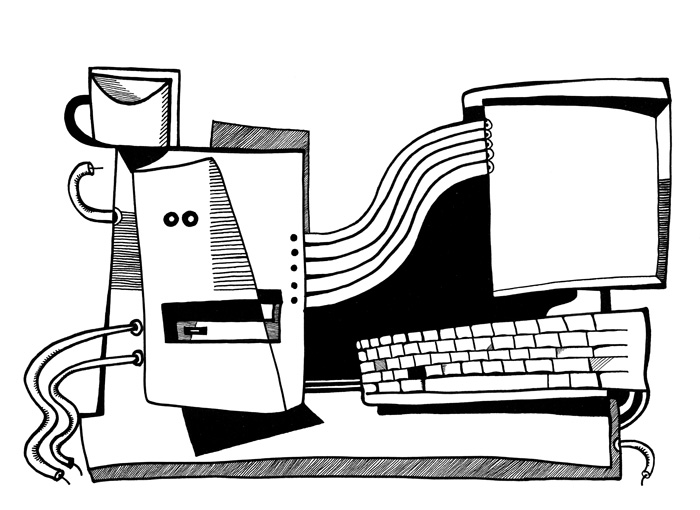
\includegraphics[scale=\FigScale]{cover4.jpg}
\end{figure}

\vspace*{\fill}
\end{center}

\clearpage

% chapters here
\chapter{\EN{Task manager practical joke}\RU{Шутка с task manager} (Windows Vista)}
\index{Windows!Windows Vista}

\RU{Посмотрим, сможем ли мы немного хакнуть Task Manager, чтобы он находил больше ядер в \ac{CPU}, чем присутствует.}%
\EN{Let's see if it's possible to hack Task Manager slightly so it would detect more \ac{CPU} cores.}

\index{Windows!NTAPI}
\RU{В начале задумаемся, откуда Task Manager знает количество ядер?}
\EN{Let us first think, how does the Task Manager know the number of cores?}
\RU{В win32 имеется функция \TT{GetSystemInfo()}, при помощи которой можно узнать.}
\EN{There is the \TT{GetSystemInfo()} win32 function present in win32 userspace which can tell us this.}
\RU{Но она не импортируется в}\EN{But it's not imported in} \TT{taskmgr.exe}.
\RU{Есть еще одна в \gls{NTAPI}, \TT{NtQuerySystemInformation()}, которая используется в 
\TT{taskmgr.exe} в ряде мест.}
\EN{There is, however, another one in \gls{NTAPI}, \TT{NtQuerySystemInformation()}, 
which is used in \TT{taskmgr.exe} in several places.}
\RU{Чтобы узнать количество ядер, нужно вызвать эту функцию с константной \TT{SystemBasicInformation} в 
первом аргументе (а это ноль}
\EN{To get the number of cores, one has to call this function with the \TT{SystemBasicInformation} constant
as a first argument (which is zero}
\footnote{\href{http://go.yurichev.com/17251}{MSDN}}).

\RU{Второй аргумент должен указывать на буфер, который примет всю информацию.}
\EN{The second argument has to point to the buffer which is getting all the information.}

\RU{Так что нам нужно найти все вызовы функции \TT{NtQuerySystemInformation(0, ?, ?, ?)}.}
\EN{So we need to find all calls to the \TT{NtQuerySystemInformation(0, ?, ?, ?)} function.}
\RU{Откроем}\EN{Let's open} \TT{taskmgr.exe} \InENRU IDA. 
\index{Windows!PDB}
\RU{Что всегда хорошо с исполняемыми файлами от Microsoft, это то что IDA может скачать соответствующуий 
\gls{PDB}-файл именно для этого файла и добавить все имена функций.}
\EN{What is always good about Microsoft executables is that IDA can download the corresponding \gls{PDB} 
file for this executable and show all function names.}
\RU{Видимо, Task Manager написан на \Cpp и некоторые функции и классы имеют говорящие за себя имена.}
\EN{It is visible that Task Manager is written in \Cpp and some of the function names and classes are really 
speaking for themselves.}
\RU{Тут есть классы}\EN{There are classes} CAdapter, CNetPage, CPerfPage, CProcInfo, CProcPage, CSvcPage, 
CTaskPage, CUserPage.
\RU{Должно быть, каждый класс соответствует каждой вкладке в Task Manager.}
\EN{Apparently, each class corresponds to each tab in Task Manager.}

\RU{Пройдемся по всем вызовам и добавим комментарий с числом, передающимся как первый аргумент.}%
\EN{Let's visit each call and add comment with the value which is passed as the first function argument.}
\RU{В некоторых местах напишем \q{not zero}, потому что значение в тех местах однозначно не ноль, 
но что-то другое (больше об этом во второй части главы).}%
\EN{We will write \q{not zero} at some places, because the value there was clearly not zero, 
but something really different (more about this in the second part of this chapter).}
\RU{А мы все-таки ищем ноль передаваемый как аргумент.}
\EN{And we are looking for zero passed as argument, after all.}

\begin{figure}[H]
\centering
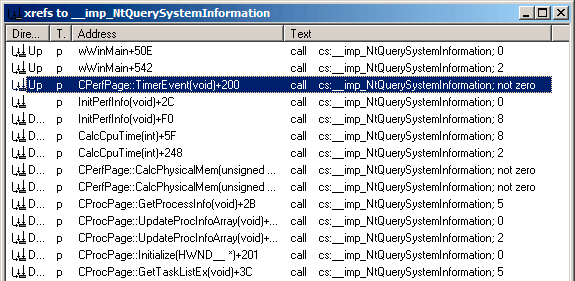
\includegraphics[scale=\FigScale]{examples/taskmgr/IDA_xrefs.png}
\caption{IDA: \RU{вызовы функции}\EN{cross references to} NtQuerySystemInformation()}
\end{figure}

\RU{Да, имена действительно говорящие сами за себя.}
\EN{Yes, the names are really speaking for themselves.}

\RU{Когда мы внимательно изучим каждое место, где вызывается \TT{NtQuerySystemInformation(0, ?, ?, ?)},
то быстро найдем то что нужно в функции \TT{InitPerfInfo()}:}%
\EN{When we closely investigate each place where \TT{NtQuerySystemInformation(0, ?, ?, ?)} is called,
we quickly find what we need in the \TT{InitPerfInfo()} function:}

\lstinputlisting[caption=taskmgr.exe (Windows Vista)]{examples/taskmgr/taskmgr.lst}

\TT{g\_cProcessors} \RU{это глобальная переменная и это имя присвоено IDA в соответствии с \gls{PDB}-файлом,
скачанным с сервера символов Microsoft}\EN{is a global variable, and this name was assigned by 
IDA according to the \gls{PDB} loaded from Microsoft's symbol server}.

\RU{Байт берется из}\EN{The byte is taken from} \TT{var\_C20}. 
\RU{И}\EN{And} \TT{var\_C58} \RU{передается в}\EN{is passed to} \TT{NtQuerySystemInformation()} 
\RU{как указатель на принимающий буфер}\EN{as a pointer to the receiving buffer}.
\RU{Разница между}\EN{The difference between} 0xC20 \AndENRU 0xC58 \RU{это}\EN{is} 0x38 (56).
\RU{Посмотрим на формат структуры, который можно найти в MSDN:}
\EN{Let's take a look at format of the return structure, which we can find in MSDN:}

\begin{lstlisting}
typedef struct _SYSTEM_BASIC_INFORMATION {
    BYTE Reserved1[24];
    PVOID Reserved2[4];
    CCHAR NumberOfProcessors;
} SYSTEM_BASIC_INFORMATION;
\end{lstlisting}

\RU{Это система x64, так что каждый PVOID занимает здесь 8 байт.}
\EN{This is a x64 system, so each PVOID takes 8 byte.}
\RU{Так что все \IT{reserved}-поля занимают $24+4*8=56$.}
\EN{All \IT{reserved} fields in the structure take $24+4*8=56$ bytes.}
\RU{О да, это значит, что \TT{var\_C20} в локальном стеке это именно поле
\TT{NumberOfProcessors} структуры \TT{SYSTEM\_BASIC\_INFORMATION}.}
\EN{Oh yes, this implies that \TT{var\_C20} is the local stack is exactly the
\TT{NumberOfProcessors} field of the \TT{SYSTEM\_BASIC\_INFORMATION} structure.}

\RU{Проверим нашу догадку}\EN{Let's check our guess}.
\RU{Скопируем}\EN{Copy} \TT{taskmgr.exe} \RU{из}\EN{from} \TT{C:\textbackslash{}Windows\textbackslash{}System32} 
\RU{в какую-нибудь другую папку}\EN{to some other folder} 
(\RU{чтобы}\EN{so the} \IT{Windows Resource Protection} \RU{не пыталась восстанавливать измененный}
\EN{will not try to restore the patched} \TT{taskmgr.exe}).

\RU{Откроем его в Hiew и найдем это место:}
\EN{Let's open it in Hiew and find the place:}

\begin{figure}[H]
\centering
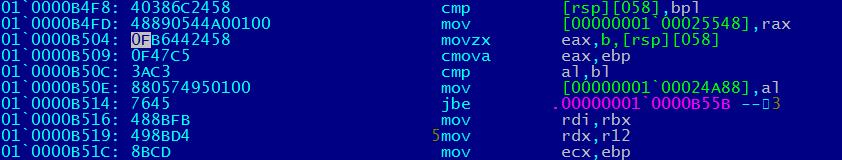
\includegraphics[scale=\FigScale]{examples/taskmgr/hiew2.png}
\caption{Hiew: \RU{найдем это место}\EN{find the place to be patched}}
\end{figure}

\RU{Заменим инструкцию \TT{MOVZX} на нашу.}
\EN{Let's replace the \TT{MOVZX} instruction with ours.}
\RU{Сделаем вид что у нас 64 ядра процессора}\EN{Let's pretend we've got 64 CPU cores}.
\RU{Добавим дополнительную инструкцию \ac{NOP} (потому что наша инструкция короче чем та что там сейчас):}
\EN{Add one additional \ac{NOP} (because our instruction is shorter than the original one):}

\begin{figure}[H]
\centering
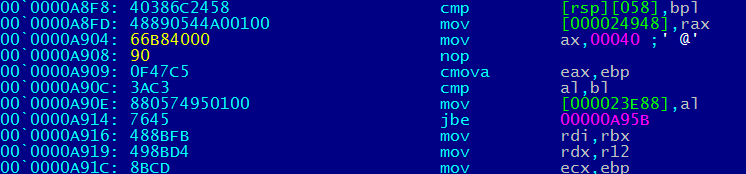
\includegraphics[scale=\FigScale]{examples/taskmgr/hiew1.png}
\caption{Hiew: \RU{меняем инструкцию}\EN{patch it}}
\end{figure}

\RU{И это работает}\EN{And it works}!
\RU{Конечно же, данные в графиках неправильные}\EN{Of course, the data in the graphs is not correct}.
\RU{Иногда, Task Manager даже показывает общую загрузку CPU более 100\%.}
\EN{At times, Task Manager even shows an overall CPU load of more than 100\%.}

\begin{figure}[H]
\centering
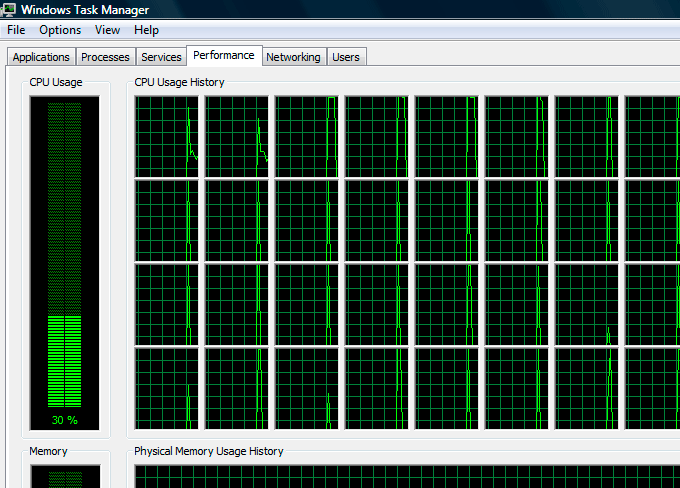
\includegraphics[scale=\FigScale]{examples/taskmgr/taskmgr_64cpu_crop.png}
\caption{\RU{Обманутый}\EN{Fooled} Windows Task Manager}
\end{figure}

\RU{Самое большое число, при котором Task Manager не падает, это 64.}%
\EN{The biggest number Task Manager is not crashes with is 64.}
\RU{Должно быть, Task Manager в Windows Vista не тестировался на компьютерах с большим количеством ядер.}
\EN{Apparently, Task Manager in Windows Vista was not tested on computers with a large number of cores.}
\RU{И, наверное, там есть внутри какие-то статичные структуры данных, ограниченные до 64-х ядер.}
\EN{So there are probably some static data structures inside it limited to 64 cores.}

\section{\RU{Использование LEA для загрузки значений}\EN{Using LEA to load values}}
\label{TaskMgr_LEA}

\RU{Иногда, \TT{LEA} используется в \TT{taskmgr.exe} вместо \TT{MOV} для установки первого аргумента 
\TT{NtQuerySystemInformation()}:}
\EN{Sometimes, \TT{LEA} is used in \TT{taskmgr.exe} instead of \TT{MOV} to set the first argument of 
\TT{NtQuerySystemInformation()}:}

\lstinputlisting[caption=taskmgr.exe (Windows Vista)]{examples/taskmgr/taskmgr2.lst}

\index{x86!\Instructions!LEA}
\RU{Честно говоря, не ясно почему, но \ac{MSVC} часто так делает.}%
\EN{It's hard to say why, but it is what \ac{MSVC} often does.}
\RU{Может быть, это какая-то оптимизация и \TT{LEA} работает быстрее или лучше, чем загрузка значения 
используя \TT{MOV}?}
\EN{Maybe this is some kind of optimization and \TT{LEA} works faster or better than loading
values using \TT{MOV}?}

\RU{Еще один пример подобного}\EN{Another example of such thing is}: 
\myref{using_MOV_and_pack_of_LEA_to_load_values}.

\clearpage
\chapter{\RU{Шутка с игрой Color Lines}\EN{Color Lines game practical joke}}
\label{chap:color_lines}

\RU{Это очень популярная игра с большим количеством реализаций}\EN{This is a very popular game with several 
implementations in existence}.
\RU{Возьмем одну из них, с названием}\EN{We can take one of them, called} BallTriX, \RU{от}\EN{from} 1997, 
\RU{доступную бесплатно на}\EN{available freely at} 
\url{http://go.yurichev.com/17311}.
\RU{Вот как она выглядит}\EN{Here is how it looks}:

\begin{figure}[H]
\centering
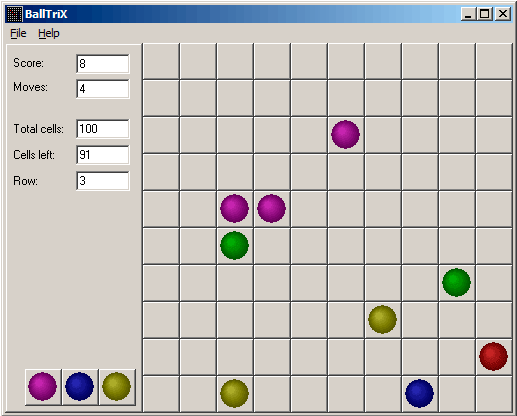
\includegraphics[scale=\FigScale]{examples/lines/1.png}
\caption{\RU{Обычный вид игры}\EN{How this game looks usually}}
\label{fig:lines_1}
\end{figure}

\clearpage
\index{\CStandardLibrary!rand()}
\RU{Посмотрим, сможем ли мы найти генератор псевдослучайных чисел и и сделать с ним одну шутку.}
\EN{So let's see, is it be possible to find the random generator and do some trick with it.}
\IDA \RU{быстро распознает стандартную функцию}\EN{quickly recognize the standard} \TT{\_rand} \RU{в}\EN{function in} 
\TT{balltrix.exe} \RU{по адресу}\EN{at} \TT{0x00403DA0}.
\IDA \RU{также показывает, что она вызывается только из одного места}\EN{also shows that it is called 
only from one place}:

\lstinputlisting{examples/lines/random.lst}

\RU{Назовем её}\EN{We'll call it} \q{random}.
\RU{Пока не будем концентрироваться на самом коде функции}\EN{Let's not to dive into this function's code yet}.

\RU{Эта функция вызывается из трех мест}\EN{This function is referred from 3 places}.

\RU{Вот первые два}\EN{Here are the first two}:

\lstinputlisting{examples/lines/1.lst}

\EN{Here is the third one}\RU{Вот третье}:

\lstinputlisting{examples/lines/2.lst}

\RU{Так что у функции только один аргумент}\EN{So the function has only one argument}.
\RU{10 передается в первых двух случаях и 5 в третьем.}
\EN{10 is passed in first two cases and 5 in third.}
\RU{Мы также можем заметить, что размер доски 10*10 и здесь 5 возможных цветов}\EN{We can also notice 
that the board has a size of 10*10 and there are 5 possible colors}.
\RU{Это оно}\EN{This is it}!
\RU{Стандартная функция}\EN{The standard} \TT{rand()} \RU{возвращает число в пределах}\EN{function returns 
a number in the} \TT{0..0x7FFF} \RU{и это неудобно, так что многие программисты пишут свою функцию,
возвращающую случайное число в некоторых заданных пределах}\EN{range and this is often inconvenient,
so many programmers implement their own random functions which returns a random number in a specified range}.
\RU{В нашем случае, предел это}\EN{In our case, the range is} $0..n-1$ \AndENRU $n$ \RU{передается как
единственный аргумент в функцию}\EN{is passed as the sole argument of the function}.
\RU{Мы можем быстро проверить это в отладчике}\EN{We can quickly check this in any debugger}.

\RU{Сделаем так, чтобы третий вызов функции всегда возвращал ноль}\EN{So let's fix the third function call to always return zero}.
\RU{В начале заменим три инструкции}\EN{First, we will replace three instructions} (\TT{PUSH/CALL/ADD}) 
\RU{на}\EN{by} \ac{NOP}s.
\RU{Затем добавим инструкцию}\EN{Then we'll add} \INS{XOR EAX, EAX}\RU{, для очистки регистра \EAX}\EN{ instruction, 
to clear the \EAX register}.

\lstinputlisting{examples/lines/fixed.lst}

\RU{Что мы сделали, это заменили вызов функции}\EN{So what we did is we replaced a call to the} \TT{random()} 
\RU{на код, всегда возвращающий ноль}\EN{function by a code which always returns zero}.

\clearpage
\RU{Теперь запустим}\EN{Let's run it now}:

\begin{figure}[H]
\centering
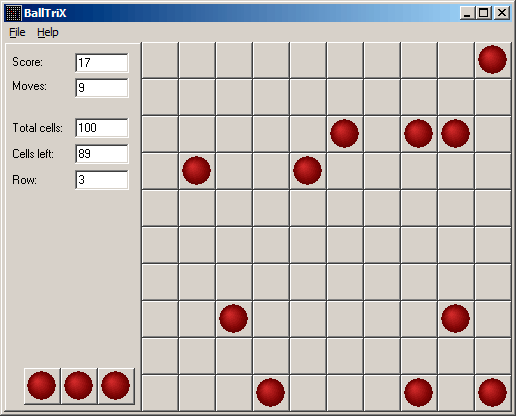
\includegraphics[scale=\FigScale]{examples/lines/2.png}
\caption{\RU{Шутка сработала}\EN{Practical joke works}}
\end{figure}

\RU{О да, это работает}\EN{Oh yes, it works}\footnote{\RU{Автор этой книги однажды сделал это как 
шутку для его сотрудников, в надежде что они перестанут играть. 
Надежды не оправдались.}\EN{Author of this book once did this as a joke for his coworkers with 
the hope that they would stop playing. They didn't.}}.

\RU{Но почему аргументы функции}\EN{But why are the arguments to the} \TT{random()} \RU{это глобальные 
переменные}\EN{functions global variables}?
\RU{Это просто потому что в настройках игры можно изменять размер доски, так что эти параметры не 
фиксированы}\EN{That's just because it's possible to change the board size in the game's settings, 
so these values are not hardcoded}.
\EN{The }10 \AndENRU 5 \RU{это просто значения по умолчанию}\EN{values are just defaults}.

\chapter{\MinesweeperWinXPExampleChapterName}
\label{minesweeper_winxp}
\index{Windows!Windows XP}

\RU{Для тех, кто не очень хорошо играет в Сапёра (Minesweeper), можно попробовать найти все скрытые мины в отладчике.}%
\EN{For those who is not very good at playing Minesweeper, we could try to reveal the hidden mines in the debugger.}

\index{\CStandardLibrary!rand()}
\index{Windows!PDB}
\RU{Как мы знаем, Сапёр располагает мины случайным образом, так что там должен быть генератор случайных чисел
или вызов стандартной функции Си \TT{rand()}.}
\EN{As we know, Minesweeper places mines randomly, so there has to be some kind of random number generator or
a call to the standard \TT{rand()} C-function.}
\RU{Вот что хорошо в реверсинге продуктов от Microsoft, так это то что часто есть \gls{PDB}-файл со всеми
символами (имена функций, \etc{}.).}
\EN{What is really cool about reversing Microsoft products is that there are \gls{PDB} 
file with symbols (function names, \etc{}).}
\RU{Когда мы загружаем}\EN{When we load} \TT{winmine.exe} \RU{в}\EN{into} \IDA, \RU{она скачивает}\EN{it downloads the} 
\gls{PDB} \RU{файл именно для этого исполняемого файла и добавляет все имена}\EN{file exactly for this 
executable and shows all names}.

\RU{И вот оно, только один вызов}\EN{So here it is, the only call to} \TT{rand()} \RU{в этой 
функции}\EN{is this function}:

\begin{lstlisting}
.text:01003940 ; __stdcall Rnd(x)
.text:01003940 _Rnd@4          proc near               ; CODE XREF: StartGame()+53
.text:01003940                                         ; StartGame()+61
.text:01003940
.text:01003940 arg_0           = dword ptr  4
.text:01003940
.text:01003940                 call    ds:__imp__rand
.text:01003946                 cdq
.text:01003947                 idiv    [esp+arg_0]
.text:0100394B                 mov     eax, edx
.text:0100394D                 retn    4
.text:0100394D _Rnd@4          endp
\end{lstlisting}

\RU{Так её назвала \IDA и это было имя данное ей разработчиками Сапёра.}
\EN{\IDA named it so, and it was the name given to it by Minesweeper's developers.}

\RU{Функция очень простая}\EN{The function is very simple}:

\begin{lstlisting}
int Rnd(int limit)
{
    return rand() % limit;
};
\end{lstlisting}

\RU{(В \gls{PDB}-файле не было имени \q{limit}; это мы назвали этот аргумент так, вручную.)}
\EN{(There was no \q{limit} name in the \gls{PDB} file; we manually named this argument like this.)}

\RU{Так что она возвращает случайное число в пределах от нуля до заданного предела}\EN{So it returns 
a random value from 0 to a specified limit}.

\TT{Rnd()} \RU{вызывается только из одного места, это функция с названием}\EN{is called only from one place, 
a function called} \TT{StartGame()}, 
\RU{и как видно, это именно тот код, что расставляет мины}\EN{and as it seems, this is exactly 
the code which place the mines}:

\begin{lstlisting}
.text:010036C7                 push    _xBoxMac
.text:010036CD                 call    _Rnd@4          ; Rnd(x)
.text:010036D2                 push    _yBoxMac
.text:010036D8                 mov     esi, eax
.text:010036DA                 inc     esi
.text:010036DB                 call    _Rnd@4          ; Rnd(x)
.text:010036E0                 inc     eax
.text:010036E1                 mov     ecx, eax
.text:010036E3                 shl     ecx, 5          ; ECX=ECX*32
.text:010036E6                 test    _rgBlk[ecx+esi], 80h
.text:010036EE                 jnz     short loc_10036C7
.text:010036F0                 shl     eax, 5          ; EAX=EAX*32
.text:010036F3                 lea     eax, _rgBlk[eax+esi]
.text:010036FA                 or      byte ptr [eax], 80h
.text:010036FD                 dec     _cBombStart
.text:01003703                 jnz     short loc_10036C7
\end{lstlisting}

\RU{Сапёр позволяет задать размеры доски, так что X (xBoxMac) и Y (yBoxMac) это глобальные переменные.}
\EN{Minesweeper allows you to set the board size, so the X (xBoxMac) and Y (yBoxMac) of the board are global variables.}
\RU{Они передаются в}\EN{They are passed to} \TT{Rnd()} \RU{и генерируются случайные координаты}\EN{and random 
coordinates are generated}.
\RU{Мина устанавливается инструкцией}\EN{A mine is placed by the} \TT{OR} \RU{на}\EN{instruction at} \TT{0x010036FA}. 
\RU{И если она уже была установлена до этого}\EN{And if it was placed before} 
(\RU{это возможно, если пара функций}\EN{it's possible if the pair of} \TT{Rnd()} 
\RU{сгенерирует пару, которая уже была сгенерирована}\EN{generates a coordinates pair which was already 
was generated}), 
\RU{тогда}\EN{then} \TT{TEST} \AndENRU \TT{JNZ} \RU{на}\EN{at} \TT{0x010036E6} 
\RU{перейдет на повторную генерацию пары}\EN{jumps to the generation routine again}.

\TT{cBombStart} \RU{это глобальная переменная, содержащая количество мин. Так что это цикл.}
\EN{is the global variable containing total number of mines. So this is loop.}

\RU{Ширина двухмерного массива это 32 (мы можем это вывести, глядя на инструкцию \TT{SHL}, которая умножает
одну из координат на 32)}\EN{The width of the array is 32 
(we can conclude this by looking at the \TT{SHL} instruction, which multiplies one of the coordinates by 32)}.

\RU{Размер глобального массива}\EN{The size of the} \TT{rgBlk} 
\RU{можно легко узнать по разнице между меткой}\EN{global array can be easily determined by the difference 
between the} \TT{rgBlk} 
\RU{в сегменте данных и следующей известной меткой}\EN{label in the data segment and the next known one}. 
\RU{Это}\EN{It is} 0x360 (864):

\begin{lstlisting}
.data:01005340 _rgBlk          db 360h dup(?)          ; DATA XREF: MainWndProc(x,x,x,x)+574
.data:01005340                                         ; DisplayBlk(x,x)+23
.data:010056A0 _Preferences    dd ?                    ; DATA XREF: FixMenus()+2
...
\end{lstlisting}

$864/32=27$.

\RU{Так что размер массива}\EN{So the array size is} $27*32$?
\RU{Это близко к тому что мы знаем: если попытаемся установить размер доски в установках Сапёра на $100*100$, то он установит размер $24*30$}%
\EN{It is close to what we know: when we try to set board size to $100*100$ in Minesweeper settings, it fallbacks to a board of size $24*30$}.
\RU{Так что это максимальный размер доски здесь}\EN{So this is the maximal board size here}.
\RU{И размер массива фиксирован для доски любого размера}\EN{And the array has a fixed size for any board size}.

\RU{Посмотрим на всё это в}\EN{So let's see all this in} \olly.
\RU{Запустим Сапёр, присоединим (attach) \olly к нему и увидим содержимое памяти по адресу где массив \TT{rgBlk} (\TT{0x01005340})}%
\EN{We will ran Minesweeper, attaching \olly to it and now we can see the memory dump at the address of the \TT{rgBlk} array (\TT{0x01005340})}
\footnote{\RU{Все адреса здесь для Сапёра под}\EN{All addresses here are for Minesweeper for} Windows XP SP3 English. 
\RU{Они могут отличаться для других сервис-паков}\EN{They may differ for other service packs}.}.

\RU{Так что у нас выходит такой дамп памяти массива}\EN{So we got this memory dump of the array}:

\lstinputlisting{examples/minesweeper/1.lst}

\olly, \RU{как и любой другой шестнадцатеричный редактор, показывает 16 байт на строку}\EN{like any other 
hexadecimal editor, shows 16 bytes per line}.
\RU{Так что каждая 32-байтная строка массива занимает ровно 2 строки}\EN{So each 32-byte array row occupies
exactly 2 lines here}.

\RU{Это уровень для начинающих (доска 9*9)}\EN{This is beginner level (9*9 board)}.

\RU{Тут еще какая-то квадратная структура, заметная визуально (байты 0x10)}\EN{There is some square 
structure can be seen visually (0x10 bytes)}.

\RU{Нажмем \q{Run} \InENRU \olly чтобы разморозить процесс Сапёра, потом нажмем в случайное место окна Сапёра, попадаемся на мине, но теперь
видны все мины}%
\EN{We will click \q{Run} \InENRU \olly to unfreeze the Minesweeper process, then we'll clicked randomly at the Minesweeper window 
and trapped into mine, but now all mines are visible}:

\begin{figure}[H]
\centering
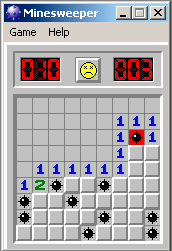
\includegraphics[scale=\FigScale]{examples/minesweeper/1.png}
\caption{\RU{Мины}\EN{Mines}}
\label{fig:minesweeper1}
\end{figure}

\RU{Сравнивая места с минами и дамп, мы можем обнаружить что 0x10 это граница, 0x0F\EMDASH{}пустой блок, 
0x8F\EMDASH{}мина.}
\EN{By comparing the mine places and the dump, we can conclude that 0x10 stands for border, 0x0F\EMDASH{}empty block, 0x8F---mine.}

\RU{Теперь добавим комментариев и также заключим все байты 0x8F в квадратные скобки:}%
\EN{Now we'll add comments and also enclose all 0x8F bytes into square brackets:}

\lstinputlisting{examples/minesweeper/2.lst}

\RU{Теперь уберем все байты связанные с границами (0x10) и всё что за ними:}%
\EN{Now we'll remove all \IT{border bytes} (0x10) and what's beyond those:}

\lstinputlisting{examples/minesweeper/3.lst}

\RU{Да, это всё мины, теперь это очень хорошо видно, в сравнении со скриншотом.}
\EN{Yes, these are mines, now it can be clearly seen and compared with the screenshot.}

\clearpage
\RU{Вот что интересно, это то что мы можем модифицировать массив прямо в \olly.}%
\EN{What is interesting is that we can modify the array right in \olly.}
\RU{Уберем все мины заменив все байты 0x8F на 0x0F, и вот что получится в Сапёре}%
\EN{We can remove all mines by changing all 0x8F bytes by 0x0F, and here is what we'll get in Minesweeper}:

\begin{figure}[H]
\centering
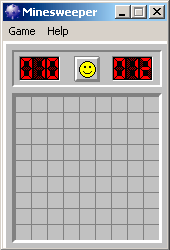
\includegraphics[scale=\FigScale]{examples/minesweeper/3.png}
\caption{\RU{Все мины убраны в отладчике}\EN{All mines are removed in debugger}}
\label{fig:minesweeper3}
\end{figure}

\RU{Также уберем их все и добавим их в первом ряду}\EN{We can also move all of them to the first line}: 

\begin{figure}[H]
\centering
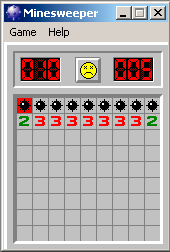
\includegraphics[scale=\FigScale]{examples/minesweeper/2.png}
\caption{\RU{Мины, установленные в отладчике}\EN{Mines set in debugger}}
\label{fig:minesweeper2}
\end{figure}

\RU{Отладчик не очень удобен для подсматривания (а это была наша изначальная цель), так что напишем маленькую
утилиту для показа содержимого доски:}%
\EN{Well, the debugger is not very convenient for eavesdropping (which was our goal anyway), so we'll write a small utility
to dump the contents of the board:}

\lstinputlisting{examples/minesweeper/minesweeper_cheater.c}

\RU{Просто установите}\EN{Just set the} \ac{PID}
\footnote{PID \RU{можно увидеть в}\EN{it can be seen in} Task Manager 
(\RU{это можно включить в}\EN{enable it in} \q{View $\rightarrow$ Select Columns})} 
\RU{и адрес массива}\EN{and the address of the array} (\TT{0x01005340} \RU{для}\EN{for} Windows XP SP3 English) 
\RU{и она покажет его}\EN{and it will dump it}
\footnote{\RU{Скомпилированная версия здесь}\EN{The compiled executable is here}: 
\href{http://go.yurichev.com/17165}{beginners.re}}.

\RU{Она подключается к win32-процессу по \ac{PID}-у и просто читает из памяти процесса по этому адресу.}
\EN{It attaches itself to a win32 process by \ac{PID} and just reads process memory an the address.}

\section{\Exercises}

\begin{itemize}

\item \RU{Почему байты описывающие границы (0x10) присутствуют вообще?}
\EN{Why do the \IT{border bytes} (0x10) exist in the array?}
\RU{Зачем они нужны, если они вообще не видимы в интерфейсе Сапёра?}
\EN{What they are for if they are not visible in Minesweeper's interface?}
\RU{Как можно обойтись без них}\EN{How could it work without them}?

\item \RU{Как выясняется, здесь больше возможных значений (для открытых блоков, для тех на которых игрок установил
	флажок, \etc{}.).}
	\EN{As it turns out, there are more values possible (for open blocks, for flagged by user, \etc{}).}
\RU{Попробуйте найти значение каждого}\EN{Try to find the meaning of each one}.

\item \RU{Измените мою утилиту так, чтобы она в запущенном процессе Сапёра убирала все мины, 
или расставляла их в соответствии с каким-то заданным шаблоном.}
\EN{Modify my utility so it can remove all mines or set them in a fixed pattern that you want in the Minesweeper
process currently running.}

\item \RU{Измените мою утилиту так, чтобы она работала без задаваемого адреса массива и без \gls{PDB}-файла.}
\EN{Modify my utility so it can work without the array address specified and without a \gls{PDB} file.}
\RU{Да, вполне возможно автоматически найти информацию о доске в сегменте данных в запущенном процессе Сапёра.}
\EN{Yes, it's possible to find board information in the data segment of Minesweeper's running process automatically.}
\RU{Подсказка}\EN{Hint}: \myref{minesweeper_winxp_hint}.

\end{itemize}

\chapter{\RU{Ручная декомпиляция + использование SMT-солвера Z3}
\EN{Hand decompiling + Z3 SMT solver}}
\index{Z3}

\RU{Любительская криптография обычно (непреднамеренно) очень слабая и может быть легко сломана ---
для криптографов, конечно}\EN{Amateur cryptography is usually (unintentionally) 
very weak and can be broken easily---for cryptographers, of course}.

\RU{Но представим на время что мы не в числе этих профессионалов}
\EN{But let's pretend we are not among these crypto-professionals}.

\RU{Вот необратимая хэш-функцию (читайте больше о них: \myref{hash_func}), 
которая конвертирует одно 64-битное значение в другое,
и нам нужно попытаться развернуть её работу назад.}
\EN{Here is one-way hash function (read more about them: \myref{hash_func}),
that converted a 64-bit value to another and we need to try
to reverse its flow back.}

\section{\RU{Ручная декомпиляция}\EN{Hand decompiling}}

\RU{Вот листинг на ассемблере в}\EN{Here its assembly language listing in} \IDA:

\lstinputlisting{examples/z3/algo_1.asm}

\RU{Пример был скомпилирован в}\EN{The example was compiled by} GCC, \RU{так что первый аргумент
передается в}\EN{so the first argument is passed in} \ECX.

\index{Hex-Rays}
\RU{Если вы не имеете}\EN{If you don't have} Hex-Rays\RU{, либо вы не доверяете его результатам, мы можем попробовать
переписать всё это на Си вручную}\EN{  or if you distrust to it, 
you can try to reverse this code manually}.
\RU{Один из методов, это представить регистры \ac{CPU} в виде локальных переменных Си и заменить каждую инструкцию
эквивалентным выражением, например}\EN{One method is to represent the \ac{CPU} registers as local C variables and 
replace each instruction by a one-line equivalent expression, like}:

\lstinputlisting{examples/z3/algo_2.c}

\RU{Если быть очень аккуратным, этот код можно скомпилировать, и он даже будет работать, 
точно так же, как оригинальный.}
\EN{If you are careful enough, 
this code can be compiled and will even work in the same way as the original.}

\RU{Затем, будем переписывать его постепенно, не забывая об использовании регистров.}
\EN{Then, we are going to rewrite it gradually, keeping in mind all registers usage.}
\RU{Внимание и фокусирование здесь крайне важно --- любая самая мелкая опечатка может испортить всю работу}
\EN{Attention and focus is very important here---any tiny typo may ruin all your work}!

\RU{Первый шаг}\EN{Here is the first step}:

\lstinputlisting{examples/z3/algo_3.c}

\RU{Следующий шаг}\EN{Next step}:

\lstinputlisting{examples/z3/algo_4.c}

\RU{Мы находим деление через умножение}\EN{We can spot the division using multiplication} (\myref{sec:divisionbynine}).
\index{Wolfram Mathematica}
\RU{Действительно, найдем делитель в}\EN{Indeed, let's calculate the divider in} Wolfram Mathematica:

\begin{lstlisting}[caption=Wolfram Mathematica]
In[1]:=N[2^(64 + 5)/16^^8888888888888889]
Out[1]:=60.
\end{lstlisting}

\RU{Получаем}\EN{We get this}:

\lstinputlisting{examples/z3/algo_5.c}

\RU{Еще один шаг}\EN{One more step}:

\lstinputlisting{examples/z3/algo_6.c}

\RU{Простым сокращением, мы видим, что вычислялось вовсе не \glslink{quotient}{частное}, а остаток от деления}
\EN{By simple reducing, we finally see that it's calculating the remainder, not the \gls{quotient}}:

\lstinputlisting{examples/z3/algo_7.c}

\RU{Заканчиваем на приятно отформатированном исходном коде}\EN{We end up with this fancy formatted source-code}:

\lstinputlisting{examples/z3/algo_src.c}

\RU{Так как мы не криптоаналитики, мы не можем найти простой способ найти входное значение
для определенного выходного значения}\EN{Since we are not cryptoanalysts we can't find an easy way to 
generate the input value for some specific output value}.
\RU{Коэффициенты инструкций сдвигов выглядят очень пугающе --- это гарантия что функция не биективная,
она имеет коллизии, или, говоря проще, возможны несколько значений на входе для одного на выходе}
\EN{The rotate instruction's coefficients look frightening---it's a warranty that the function is not bijective,
it has collisions, or, speaking more simply, many inputs may be possible for one output}.

\RU{Брут-форс это тоже не решение, т.к., значения 64-битные, и это совершенно нереально}
\EN{Brute-force is not solution because values are 64-bit ones, that's beyond reality}.

\section{\RU{Попробуем Z3 SMT-солвер}\EN{Now let's use the Z3 SMT solver}}
\index{Z3}

\RU{Но все же, без всяких специальных знаний из криптографии, мы можем попытаться взломать алгоритм при помощи
великолепного SMT-солвера от}\EN{Still, without any special cryptographic knowledge, we may try to break this 
algorithm using the excellent SMT solver from} Microsoft Research \RU{под названием}\EN{named} 
Z3\footnote{\url{http://go.yurichev.com/17314}}.
\RU{На самом деле, это автоматический доказыватель теорем, 
но мы будем использовать его как SMT-солвер.}
\EN{It is in fact theorem prover, but we are going to use it as SMT solver.}
\RU{Упрощенно говоря, мы можем думать о нем как о системе, способной решать очень большие системы уравнений}
\EN{Simply said, we can think about it as a system capable of solving huge equation systems}.

\RU{Вот исходный код на Питоне}\EN{Here is the Python source code}:

\lstinputlisting[numbers=left]{examples/z3/1.py}

\RU{Это будет наш первый солвер}\EN{This is going to be our first solver}.

\RU{На строке 7 мы видим объявление переменных}\EN{We see the variable definitions on line 7}.
\RU{Это просто 64-битные переменные}\EN{These are just 64-bit variables}.
\TT{i1..i6} \RU{это промежуточные переменные, отражающие значения в регистрах между исполнениями инструкций}
\EN{are intermediate variables, representing the values in the registers between instruction executions}.

\RU{Потом добавляем т.н. констрайнты, в строках}\EN{Then we add the so-called constraints on lines} 10..15.
\RU{Самый последний констрайнт в строке 17 это наиболее важный: мы будем искать входное значение для
нашего алгоритма, при котором он выдаст на выходе}
\EN{The last constraint at 17 is the most important one: 
we are going to try to find an input value for which our algorithm will produce} 10816636949158156260.

\RU{Собственно, SMT-солвер ищет (любые) значения, удовлетворяющие всем констрайнтам}
\EN{Essentially, the SMT-solver searches for (any) values that satisfies all constraints}.

RotateRight, RotateLeft, URem\EMDASH{}\RU{это функции из Питоновского Z3 \ac{API} для описания выражений, 
они не связаны с ЯП Python}
\EN{are functions from the Z3 Python \ac{API}, not related to Python \ac{PL}}.

\RU{Запускаем}\EN{Then we run it}:

\begin{lstlisting}
...>python.exe 1.py
sat
[i1 = 3959740824832824396,
 i3 = 8957124831728646493,
 i5 = 10816636949158156260,
 inp = 1364123924608584563,
 outp = 10816636949158156260,
 i4 = 14065440378185297801,
 i2 = 4954926323707358301]
 inp=0x12EE577B63E80B73
outp=0x961C69FF0AEFD7E4
\end{lstlisting}

\q{sat} \RU{означает}\EN{mean} \q{satisfiable}, \RU{т.е. солвер нашел по крайней мере одно решение}
\EN{i.e., the solver was able to found at least one solution}.
\RU{Решение выведено внутри квадратных скобок}\EN{The solution is printed in the square brackets}.
\RU{Две последние строки это пара входного/выходного значения в шестнадцатеричном виде}
\EN{The last two lines are the input/output pair in hexadecimal form}.
\RU{Да, действительно, если мы запустим нашу функцию с}\EN{Yes, indeed, if we run our function with} 
\TT{0x12EE577B63E80B73} \RU{на входе, алгоритм выдаст искомое значение}
\EN{as input, the algorithm will produce the value we were looking for}.

\RU{Но, как мы заметили ранее, функция не биективная, так что тут могут быть и другие корректные входные значения}
\EN{But, as we noticed before, the function we work with is not bijective, so there may be other correct
input values}.
\RU{Z3 SMT-солвер не выдает результаты больше одного, но мы можем хакнуть наш пример немного, 
добавив констрайнт в строке 19, означая, что мы ищем какие угодно другие результаты кроме этого}
\EN{The Z3 SMT solver is not capable of producing more than one result, but let's hack our example slightly, 
by adding line 19, which implies \q{look for any other results than this}}:

\lstinputlisting[numbers=left]{examples/z3/2.py}

\RU{Действительно, получаем еще один верный результат}\EN{Indeed, it finds another correct result}:

\begin{lstlisting}
...>python.exe 2.py
sat
[i1 = 3959740824832824396,
 i3 = 8957124831728646493,
 i5 = 10816636949158156260,
 inp = 10587495961463360371,
 outp = 10816636949158156260,
 i4 = 14065440378185297801,
 i2 = 4954926323707358301]
 inp=0x92EE577B63E80B73
outp=0x961C69FF0AEFD7E4
\end{lstlisting}

\RU{Это можно автоматизировать}\EN{This can be automated}.
\RU{Каждый найденный результат можно добавлять в качестве констрайнта и искать следующий.}
\EN{Each found result can be added as a constraint and then the next result will be searched for.}
\RU{Пример немного сложнее}\EN{Here is a slightly more sophisticated example}:

\lstinputlisting[numbers=left]{examples/z3/3.py}

\RU{Получаем}\EN{We got}:

\begin{lstlisting}
1364123924608584563
1234567890
9223372038089343698
4611686019661955794
13835058056516731602
3096040143925676201
12319412180780452009
7707726162353064105
16931098199207839913
1906652839273745429
11130024876128521237
15741710894555909141
6518338857701133333
5975809943035972467
15199181979890748275
10587495961463360371
results total= 16
\end{lstlisting}

\RU{Так что имеется 16 верных входных значений для}\EN{So there are 16 correct input values for} 
\TT{0x92EE577B63E80B73} \RU{на выходе}\EN{as a result}.

\RU{Второй это}\EN{The second is} 1234567890\EMDASH{}\RU{действительно, это значение было использовано изначально,
при подготовке этого примера}%
\EN{it is indeed the value which was used originally while preparing this example}.

\RU{Попробуем изучить алгоритм немного больше}\EN{Let's also try to research our algorithm a bit more}.
\RU{В порыве садистских желаний, попробуем найти, есть ли здесь какая-нибудь возможная пара входов/выходов,
в которых младшие 32-битные части равны друг другу}
\EN{Acting on a sadistic whim, let's find if the there are any possible input/output pairs in 
which the lower 32-bit parts are equal to each other}?

\RU{Уберем констрайнт}\EN{Let's remove the} \IT{outp} \RU{и добавим другой, в строке 17}
\EN{constraint and add another, at line 17}:

\lstinputlisting[numbers=left]{examples/z3/4.py}

\RU{И действительно}\EN{It is indeed so}:

\begin{lstlisting}
sat
[i1 = 14869545517796235860,
 i3 = 8388171335828825253,
 i5 = 6918262285561543945,
 inp = 1370377541658871093,
 outp = 14543180351754208565,
 i4 = 10167065714588685486,
 i2 = 5541032613289652645]
 inp=0x13048F1D12C00535
outp=0xC9D3C17A12C00535
\end{lstlisting}

\RU{Можем упражняться в садизме и далее: пусть последние 16-бит всегда будут}
\EN{Let's be more sadistic and add another constraint: last the 16 bits must be} \TT{0x1234}:

\lstinputlisting[numbers=left]{examples/z3/5.py}

\RU{Это так же возможно}\EN{Oh yes, this possible as well}:

\begin{lstlisting}
sat
[i1 = 2834222860503985872,
 i3 = 2294680776671411152,
 i5 = 17492621421353821227,
 inp = 461881484695179828,
 outp = 419247225543463476,
 i4 = 2294680776671411152,
 i2 = 2834222860503985872]
 inp=0x668EEC35F961234
outp=0x5D177215F961234
\end{lstlisting}

\RU{Z3 работает крайне быстро и это означает что алгоритм слаб, и вообще не относится к криптографическим 
(как и почти вся любительская криптография)}
\EN{Z3 works very fast and it implies that the algorithm is weak, it is not cryptographic at all
(like the most of the amateur cryptography)}.

\RU{Можно ли попытаться сделать что-то подобное с настоящими криптоалгоритмами этими методами}
\EN{Is it possible to tackle real cryptography by these methods}? 
\RU{Настоящие алгоритмы, такие как}\EN{Real algorithms like} AES, RSA, \RU{\etc{}, так же могут быть представлены
в виде огромных систем уравнений, но они большие настолько, что с ними нельзя работать на компьютерах,
ни сейчас, ни в обозримом будущем}\EN{\etc{}, can also be represented as huge system of equations, 
but these are so huge that they are impossible to work with on computers, now or in the near future}.
\RU{Разумеется, криптографы об этом всем прекрасно знают}\EN{Of course, cryptographers are aware of this}.

\EN{Summarizing, when dealing with amateur crypto, 
it's a very good idea to try a SMT/SAT solver (like Z3).}
\RU{Подводя итоги, нужно сказать, что работая с любительской криптографией, 
попробовать SMT/SAT-солвер (как Z3) это всегда хорошая идея.}

\RU{Еще одна статья о Z3:}\EN{Another article about Z3 is} \cite{Rockey}.

\ifdefined\IncludeDongles
\chapter{\RU{Донглы}\EN{Dongles}}
\label{dongles}

\RU{Автор этих строк иногда делал замену \glslink{dongle}{донглам} или \q{эмуляторы донглов} 
и здесь немного примеров, как это происходит.}
\EN{Author of these lines, occasionally did software copy-protection \gls{dongle} replacements, or \q{dongle emulators} and here
are couple examples of how it's happening.}

\RU{Об одном неописанном здесь случае вы также можете прочитать здесь}
\EN{About one of the cases that is not present here, you can read here}: \cite{Rockey}.

\input{examples/dongles/1/main}
\input{examples/dongles/2/main}
\ifdefined\IncludeMSDOS
\input{examples/dongles/3/main}
\fi
\fi

\chapter{\RU{\q{QR9}: Любительская криптосистема, вдохновленная кубиком Рубика}
\EN{\q{QR9}: Rubik's cube inspired amateur crypto-algorithm}}

\RU{Любительские криптосистемы иногда встречаются довольно странные.}
\EN{Sometimes amateur cryptosystems appear to be pretty bizarre.}

\RU{Однажды автора сих строк попросили разобраться с одним таким любительским криптоалгоритмом встроенным в 
утилиту для шифрования, исходный код которой был утерян\footnote{Он также получил разрешение от 
клиента на публикацию деталей алгоритма}.}
\EN{The author of this book was once asked to reverse engineer an amateur cryptoalgorithm of some data encryption utility, 
the source code for which was lost\footnote{He also got permission from the customer to publish the algorithm's details}.}

\RU{Вот листинг этой утилиты для шифрования, полученный при помощи \IDA}%
\EN{Here is the listing exported from \IDA for the original encryption utility}:

\lstinputlisting{examples/qr9/qr9_original.lst}

\RU{Все имена функций и меток даны мною в процессе анализа.}
\EN{All function and label names were given by me during the analysis.}

\RU{Начнем с самого верха. Вот функция, берущая на вход два имени файла и пароль.}
\EN{Let's start from the top. Here is a function that takes two file names and password.}

\begin{lstlisting}
.text:00541320 ; int __cdecl crypt_file(int Str, char *Filename, int password)
.text:00541320 crypt_file      proc near
.text:00541320
.text:00541320 Str             = dword ptr  4
.text:00541320 Filename        = dword ptr  8
.text:00541320 password        = dword ptr  0Ch
.text:00541320
\end{lstlisting}

\RU{Открыть файл и сообщить об ошибке в случае ошибки:}\EN{Open the file and report if an error occurs:}

\begin{lstlisting}
.text:00541320                 mov     eax, [esp+Str]
.text:00541324                 push    ebp
.text:00541325                 push    offset Mode     ; "rb"
.text:0054132A                 push    eax             ; Filename
.text:0054132B                 call    _fopen          ; open file
.text:00541330                 mov     ebp, eax
.text:00541332                 add     esp, 8
.text:00541335                 test    ebp, ebp
.text:00541337                 jnz     short loc_541348
.text:00541339                 push    offset Format   ; "Cannot open input file!\n"
.text:0054133E                 call    _printf
.text:00541343                 add     esp, 4
.text:00541346                 pop     ebp
.text:00541347                 retn
.text:00541348
.text:00541348 loc_541348:
\end{lstlisting}

\index{\CStandardLibrary!fseek()}
\index{\CStandardLibrary!ftell()}
\RU{Узнать размер файла используя}\EN{Get the file size via} \TT{fseek()}/\TT{ftell()}:

\lstinputlisting{examples/qr9/1.\LANG}

\RU{Этот фрагмент кода вычисляет длину файла, выровненную по 64-байтной границе.
Это потому что этот алгоритм шифрования работает только с блоками размерами 64 байта.
Работает очень просто: разделить длину файла на 64, забыть об остатке, прибавить 1,
умножить на 64.
Следующий код удаляет остаток от деления, как если бы это значение уже было разделено 
на 64 и добавляет 64. Это почти то же самое.}
\EN{This fragment of code calculates the file size aligned on a 64-byte boundary. 
This is because this cryptographic algorithm works with only 64-byte blocks. 
The operation is pretty straightforward: divide the file size by 64, forget about the remainder and add 1, 
then multiply by 64. 
The following code removes the remainder as if the value was already divided by 64 and adds 64. 
It is almost the same.}

\lstinputlisting{examples/qr9/2.\LANG}

\RU{Выделить буфер с выровненным размером:}\EN{Allocate buffer with aligned size:}

\begin{lstlisting}
.text:00541373                 push    esi             ; Size
.text:00541374                 call    _malloc
\end{lstlisting}

\index{\CStandardLibrary!calloc()}
\RU{Вызвать memset(), т.е. очистить выделенный буфер\footnote{malloc() + memset() можно было бы 
заменить на calloc()}.}\EN{Call memset(), e.g., clear the allocated buffer\footnote{malloc() + memset() could 
be replaced by calloc()}.}

\lstinputlisting{examples/qr9/3.\LANG}

\RU{Чтение файла используя стандартную функцию Си}\EN{Read file via the standard C function} \TT{fread()}.

\begin{lstlisting}
.text:00541392                 mov     eax, [esp+38h+Str]
.text:00541396                 push    eax             ; ElementSize
.text:00541397                 push    ebx             ; DstBuf
.text:00541398                 call    _fread          ; read file
.text:0054139D                 push    ebp             ; File
.text:0054139E                 call    _fclose
\end{lstlisting}

\RU{Вызов \TT{crypt()}. Эта функция берет на вход буфер, длину буфера (выровненную) и строку пароля.}
\EN{Call \TT{crypt()}. This function takes a buffer, buffer size (aligned) and a password string.}

\begin{lstlisting}
.text:005413A3                 mov     ecx, [esp+44h+password]
.text:005413A7                 push    ecx             ; password
.text:005413A8                 push    esi             ; aligned size
.text:005413A9                 push    ebx             ; buffer
.text:005413AA                 call    crypt           ; do crypt
\end{lstlisting}

\RU{Создать выходной файл. Кстати, разработчик забыл вставить проверку, создался ли файл успешно!
Результат открытия файла, впрочем, проверяется.}
\EN{Create the output file. By the way, the developer forgot to check if it is was created correctly! 
The file opening result is being checked, though.}

\begin{lstlisting}
.text:005413AF                 mov     edx, [esp+50h+Filename]
.text:005413B3                 add     esp, 40h
.text:005413B6                 push    offset aWb      ; "wb"
.text:005413BB                 push    edx             ; Filename
.text:005413BC                 call    _fopen
.text:005413C1                 mov     edi, eax
\end{lstlisting}

\RU{Теперь хэндл созданного файла в регистре \EDI. Записываем сигнатуру \q{QR9}.}
\EN{The newly created file handle is in the \EDI register now. Write signature \q{QR9}.}

\begin{lstlisting}
.text:005413C3                 push    edi             ; File
.text:005413C4                 push    1               ; Count
.text:005413C6                 push    3               ; Size
.text:005413C8                 push    offset aQr9     ; "QR9"
.text:005413CD                 call    _fwrite         ; write file signature
\end{lstlisting}

\RU{Записываем настоящую длину файла (не выровненную)}\EN{Write the actual file size (not aligned)}:

\begin{lstlisting}
.text:005413D2                 push    edi             ; File
.text:005413D3                 push    1               ; Count
.text:005413D5                 lea     eax, [esp+30h+Str]
.text:005413D9                 push    4               ; Size
.text:005413DB                 push    eax             ; Str
.text:005413DC                 call    _fwrite         ; write original file size
\end{lstlisting}

\RU{Записываем шифрованный буфер}\EN{Write the encrypted buffer}:

\begin{lstlisting}
.text:005413E1                 push    edi             ; File
.text:005413E2                 push    1               ; Count
.text:005413E4                 push    esi             ; Size
.text:005413E5                 push    ebx             ; Str
.text:005413E6                 call    _fwrite         ; write encrypted file
\end{lstlisting}

\RU{Закрыть файл и освободить выделенный буфер}\EN{Close the file and free the allocated buffer}:

\begin{lstlisting}
.text:005413EB                 push    edi             ; File
.text:005413EC                 call    _fclose
.text:005413F1                 push    ebx             ; Memory
.text:005413F2                 call    _free
.text:005413F7                 add     esp, 40h
.text:005413FA                 pop     edi
.text:005413FB                 pop     esi
.text:005413FC                 pop     ebx
.text:005413FD                 pop     ebp
.text:005413FE                 retn
.text:005413FE crypt_file      endp
\end{lstlisting}

\RU{Переписанный на Си код}\EN{Here is the reconstructed C code}:

\begin{lstlisting}
void crypt_file(char *fin, char* fout, char *pw)
{
	FILE *f;
	int flen, flen_aligned;
	BYTE *buf;

	f=fopen(fin, "rb");
	
	if (f==NULL)
	{
		printf ("Cannot open input file!\n");
		return;
	};

	fseek (f, 0, SEEK_END);
	flen=ftell (f);
	fseek (f, 0, SEEK_SET);

	flen_aligned=(flen&0xFFFFFFC0)+0x40;

	buf=(BYTE*)malloc (flen_aligned);
	memset (buf, 0, flen_aligned);

	fread (buf, flen, 1, f);

	fclose (f);

	crypt (buf, flen_aligned, pw);
	
	f=fopen(fout, "wb");

	fwrite ("QR9", 3, 1, f);
	fwrite (&flen, 4, 1, f);
	fwrite (buf, flen_aligned, 1, f);

	fclose (f);

	free (buf);
};
\end{lstlisting}

\RU{Процедура дешифрования почти такая же}\EN{The decryption procedure is almost the same}:

\begin{lstlisting}
.text:00541400 ; int __cdecl decrypt_file(char *Filename, int, void *Src)
.text:00541400 decrypt_file    proc near
.text:00541400
.text:00541400 Filename        = dword ptr  4
.text:00541400 arg_4           = dword ptr  8
.text:00541400 Src             = dword ptr  0Ch
.text:00541400
.text:00541400                 mov     eax, [esp+Filename]
.text:00541404                 push    ebx
.text:00541405                 push    ebp
.text:00541406                 push    esi
.text:00541407                 push    edi
.text:00541408                 push    offset aRb      ; "rb"
.text:0054140D                 push    eax             ; Filename
.text:0054140E                 call    _fopen
.text:00541413                 mov     esi, eax
.text:00541415                 add     esp, 8
.text:00541418                 test    esi, esi
.text:0054141A                 jnz     short loc_54142E
.text:0054141C                 push    offset aCannotOpenIn_0 ; "Cannot open input file!\n"
.text:00541421                 call    _printf
.text:00541426                 add     esp, 4
.text:00541429                 pop     edi
.text:0054142A                 pop     esi
.text:0054142B                 pop     ebp
.text:0054142C                 pop     ebx
.text:0054142D                 retn
.text:0054142E
.text:0054142E loc_54142E:
.text:0054142E                 push    2               ; Origin
.text:00541430                 push    0               ; Offset
.text:00541432                 push    esi             ; File
.text:00541433                 call    _fseek
.text:00541438                 push    esi             ; File
.text:00541439                 call    _ftell
.text:0054143E                 push    0               ; Origin
.text:00541440                 push    0               ; Offset
.text:00541442                 push    esi             ; File
.text:00541443                 mov     ebp, eax
.text:00541445                 call    _fseek
.text:0054144A                 push    ebp             ; Size
.text:0054144B                 call    _malloc
.text:00541450                 push    esi             ; File
.text:00541451                 mov     ebx, eax
.text:00541453                 push    1               ; Count
.text:00541455                 push    ebp             ; ElementSize
.text:00541456                 push    ebx             ; DstBuf
.text:00541457                 call    _fread
.text:0054145C                 push    esi             ; File
.text:0054145D                 call    _fclose
\end{lstlisting}

\RU{Проверяем сигнатуру (первые 3 байта)}\EN{Check signature (first 3 bytes)}:

\begin{lstlisting}
.text:00541462                 add     esp, 34h
.text:00541465                 mov     ecx, 3
.text:0054146A                 mov     edi, offset aQr9_0 ; "QR9"
.text:0054146F                 mov     esi, ebx
.text:00541471                 xor     edx, edx
.text:00541473                 repe cmpsb
.text:00541475                 jz      short loc_541489
\end{lstlisting}

\RU{Сообщить об ошибке если сигнатура отсутствует}\EN{Report an error if the signature is absent}:

\begin{lstlisting}
.text:00541477                 push    offset aFileIsNotCrypt ; "File is not encrypted!\n"
.text:0054147C                 call    _printf
.text:00541481                 add     esp, 4
.text:00541484                 pop     edi
.text:00541485                 pop     esi
.text:00541486                 pop     ebp
.text:00541487                 pop     ebx
.text:00541488                 retn
.text:00541489
.text:00541489 loc_541489:
\end{lstlisting}

\RU{Вызвать}\EN{Call} \TT{decrypt()}.

\begin{lstlisting}
.text:00541489                 mov     eax, [esp+10h+Src]
.text:0054148D                 mov     edi, [ebx+3]
.text:00541490                 add     ebp, 0FFFFFFF9h
.text:00541493                 lea     esi, [ebx+7]
.text:00541496                 push    eax             ; Src
.text:00541497                 push    ebp             ; int
.text:00541498                 push    esi             ; int
.text:00541499                 call    decrypt
.text:0054149E                 mov     ecx, [esp+1Ch+arg_4]
.text:005414A2                 push    offset aWb_0    ; "wb"
.text:005414A7                 push    ecx             ; Filename
.text:005414A8                 call    _fopen
.text:005414AD                 mov     ebp, eax
.text:005414AF                 push    ebp             ; File
.text:005414B0                 push    1               ; Count
.text:005414B2                 push    edi             ; Size
.text:005414B3                 push    esi             ; Str
.text:005414B4                 call    _fwrite
.text:005414B9                 push    ebp             ; File
.text:005414BA                 call    _fclose
.text:005414BF                 push    ebx             ; Memory
.text:005414C0                 call    _free
.text:005414C5                 add     esp, 2Ch
.text:005414C8                 pop     edi
.text:005414C9                 pop     esi
.text:005414CA                 pop     ebp
.text:005414CB                 pop     ebx
.text:005414CC                 retn
.text:005414CC decrypt_file    endp
\end{lstlisting}

\RU{Переписанный на Си код}\EN{Here is the reconstructed C code}:

\begin{lstlisting}
void decrypt_file(char *fin, char* fout, char *pw)
{
	FILE *f;
	int real_flen, flen;
	BYTE *buf;

	f=fopen(fin, "rb");
	
	if (f==NULL)
	{
		printf ("Cannot open input file!\n");
		return;
	};

	fseek (f, 0, SEEK_END);
	flen=ftell (f);
	fseek (f, 0, SEEK_SET);

	buf=(BYTE*)malloc (flen);

	fread (buf, flen, 1, f);

	fclose (f);

	if (memcmp (buf, "QR9", 3)!=0)
	{
		printf ("File is not encrypted!\n");
		return;
	};

	memcpy (&real_flen, buf+3, 4);

	decrypt (buf+(3+4), flen-(3+4), pw);
	
	f=fopen(fout, "wb");

	fwrite (buf+(3+4), real_flen, 1, f);

	fclose (f);

	free (buf);
};
\end{lstlisting}

\RU{OK, посмотрим глубже}\EN{OK, now let's go deeper}.

\RU{Функция}\EN{Function} \TT{crypt()}:

\begin{lstlisting}
.text:00541260 crypt           proc near
.text:00541260
.text:00541260 arg_0           = dword ptr  4
.text:00541260 arg_4           = dword ptr  8
.text:00541260 arg_8           = dword ptr  0Ch
.text:00541260
.text:00541260                 push    ebx
.text:00541261                 mov     ebx, [esp+4+arg_0]
.text:00541265                 push    ebp
.text:00541266                 push    esi
.text:00541267                 push    edi
.text:00541268                 xor     ebp, ebp
.text:0054126A
.text:0054126A loc_54126A:
\end{lstlisting}

\index{x86!\Instructions!MOVSD}
\RU{Этот фрагмент кода копирует часть входного буфера во внутренний буфер, который мы позже назовем \q{cube64}.}%
\EN{This fragment of code copies a part of the input buffer to an internal array we later name \q{cube64}.}
\RU{Длина в регистре \ECX. \TT{MOVSD} означает \IT{скопировать 32-битное слово}, так что, 16 32-битных слов
это как раз 64 байта.}\EN{The size is in the \ECX register. \TT{MOVSD} stands for \IT{move 32-bit dword}, so, 
16 32-bit dwords are exactly 64 bytes.}

\begin{lstlisting}
.text:0054126A                 mov     eax, [esp+10h+arg_8]
.text:0054126E                 mov     ecx, 10h
.text:00541273                 mov     esi, ebx   ; EBX is pointer within input buffer
.text:00541275                 mov     edi, offset cube64
.text:0054127A                 push    1
.text:0054127C                 push    eax
.text:0054127D                 rep movsd
\end{lstlisting}

\RU{Вызвать}\EN{Call} \TT{rotate\_all\_with\_password()}:

\begin{lstlisting}
.text:0054127F                 call    rotate_all_with_password
\end{lstlisting}

\RU{Скопировать зашифрованное содержимое из \q{cube64} назад в буфер}
\EN{Copy encrypted contents back from \q{cube64} to buffer}:

\begin{lstlisting}
.text:00541284                 mov     eax, [esp+18h+arg_4]
.text:00541288                 mov     edi, ebx
.text:0054128A                 add     ebp, 40h
.text:0054128D                 add     esp, 8
.text:00541290                 mov     ecx, 10h
.text:00541295                 mov     esi, offset cube64
.text:0054129A                 add     ebx, 40h  ; add 64 to input buffer pointer
.text:0054129D                 cmp     ebp, eax  ; EBP contain amount of encrypted data.
.text:0054129F                 rep movsd
\end{lstlisting}

\RU{Если \EBP не больше чем длина во входном аргументе, тогда переходим к следующему блоку.}%
\EN{If \EBP is not bigger that the size input argument, then continue to the next block.}

\begin{lstlisting}
.text:005412A1                 jl      short loc_54126A
.text:005412A3                 pop     edi
.text:005412A4                 pop     esi
.text:005412A5                 pop     ebp
.text:005412A6                 pop     ebx
.text:005412A7                 retn
.text:005412A7 crypt           endp
\end{lstlisting}

\RU{Реконструированная функция \TT{crypt()}}\EN{Reconstructed \TT{crypt()} function}:

\begin{lstlisting}
void crypt (BYTE *buf, int sz, char *pw)
{
	int i=0;
	
	do
	{
		memcpy (cube, buf+i, 8*8);
		rotate_all (pw, 1);
		memcpy (buf+i, cube, 8*8);
		i+=64;
	}
	while (i<sz);
};
\end{lstlisting}

\RU{OK, углубимся в функцию \TT{rotate\_all\_with\_password()}. Она берет на вход два аргумента: 
строку пароля и число.}\EN{OK, now let's go deeper in function \TT{rotate\_all\_with\_password()}. 
It takes two arguments: password string and a number.}
\RU{В функции \TT{crypt()}, число 1 используется и в \TT{decrypt()} (где \TT{rotate\_all\_with\_password()}
функция вызывается также), число 3.}
\EN{In \TT{crypt()}, the number 1 is used, and in the \TT{decrypt()} function (where \TT{rotate\_all\_with\_password()} function 
is called too), the number is 3.}

\begin{lstlisting}
.text:005411B0 rotate_all_with_password proc near
.text:005411B0
.text:005411B0 arg_0           = dword ptr  4
.text:005411B0 arg_4           = dword ptr  8
.text:005411B0
.text:005411B0                 mov     eax, [esp+arg_0]
.text:005411B4                 push    ebp
.text:005411B5                 mov     ebp, eax
\end{lstlisting}

\RU{Проверяем символы в пароле. Если это ноль, выходим:}\EN{Check the current character in the password. If it is zero, exit:}

\begin{lstlisting}
.text:005411B7                 cmp     byte ptr [eax], 0
.text:005411BA                 jz      exit
.text:005411C0                 push    ebx
.text:005411C1                 mov     ebx, [esp+8+arg_4]
.text:005411C5                 push    esi
.text:005411C6                 push    edi
.text:005411C7
.text:005411C7 loop_begin:
\end{lstlisting}

\index{\CStandardLibrary!tolower()}
\RU{Вызываем \TT{tolower()}, стандартную функцию Си.}\EN{Call \TT{tolower()}, a standard C function.}

\begin{lstlisting}
.text:005411C7                 movsx   eax, byte ptr [ebp+0]
.text:005411CB                 push    eax             ; C
.text:005411CC                 call    _tolower
.text:005411D1                 add     esp, 4
\end{lstlisting}

\RU{Хмм, если пароль содержит символ не из латинского алфавита, он пропускается!
Действительно, если мы запускаем утилиту для шифрования используя символы не латинского алфавита, 
похоже, они просто игнорируются.}
\EN{Hmm, if the password contains non-Latin character, it is skipped! 
Indeed, when we run the encryption utility and try non-Latin characters in the password, 
they seem to be ignored.}

\begin{lstlisting}
.text:005411D4                 cmp     al, 'a'
.text:005411D6                 jl      short next_character_in_password
.text:005411D8                 cmp     al, 'z'
.text:005411DA                 jg      short next_character_in_password
.text:005411DC                 movsx   ecx, al
\end{lstlisting}

\RU{Отнимем значение \q{a} (97) от символа.}\EN{Subtract the value of \q{a} (97) from the character.}

\begin{lstlisting}
.text:005411DF                 sub     ecx, 'a'  ; 97
\end{lstlisting}

\RU{После вычитания, тут будет 0 для \q{a}, 1 для \q{b}, и так далее. И 25 для \q{z}.}
\EN{After subtracting, we'll get 0 for \q{a} here, 1 for \q{b}, etc. And 25 for \q{z}.}

\begin{lstlisting}
.text:005411E2                 cmp     ecx, 24
.text:005411E5                 jle     short skip_subtracting
.text:005411E7                 sub     ecx, 24
\end{lstlisting}

\RU{Похоже, символы \q{y} и \q{z} также исключительные.
После этого фрагмента кода, \q{y} становится 0, а \q{z} ~--- 1.
Это значит, что 26 латинских букв становятся значениями в интервале 0..23, (всего 24).}
\EN{It seems, \q{y} and \q{z} are exceptional characters too. 
After that fragment of code, \q{y} becomes 0 and \q{z}~---1. 
This implies that the 26 Latin alphabet symbols become values in the range of 0..23, (24 in total).}

\begin{lstlisting}
.text:005411EA
.text:005411EA skip_subtracting:                       ; CODE XREF: rotate_all_with_password+35
\end{lstlisting}

\RU{Это, на самом деле, деление через умножение.
Читайте об этом больше в секции \q{\DivisionByNineSectionName}~(\myref{sec:divisionbynine}).}
\EN{This is actually division via multiplication. 
You can read more about it in the \q{\DivisionByNineSectionName} section~(\myref{sec:divisionbynine}).}

\RU{Это код, на самом деле, делит значение символа пароля на 3.}
\EN{The code actually divides the password character's value by 3.}
% TODO1: add Mathematica calculations
\begin{lstlisting}
.text:005411EA                 mov     eax, 55555556h
.text:005411EF                 imul    ecx
.text:005411F1                 mov     eax, edx
.text:005411F3                 shr     eax, 1Fh
.text:005411F6                 add     edx, eax
.text:005411F8                 mov     eax, ecx
.text:005411FA                 mov     esi, edx
.text:005411FC                 mov     ecx, 3
.text:00541201                 cdq
.text:00541202                 idiv    ecx
\end{lstlisting}

\RU{\EDX\EMDASH{}остаток от деления.}\EN{\EDX is the remainder of the division.}

\lstinputlisting{examples/qr9/4.\LANG}

\RU{Если остаток 2, вызываем \TT{rotate3()}. 
\EDX это второй аргумент функции \TT{rotate\_all\_with\_password()}. 
Как мы уже заметили, 1 это для шифрования, 3 для дешифрования.
Так что здесь цикл, функции rotate1/2/3 будут вызываться столько же раз, сколько значение переменной
в первом аргументе.}
\EN{If the remainder is 2, call \TT{rotate3()}. 
\EDI is the second argument of the \TT{rotate\_all\_with\_password()} function.
As we already noted, 1 is for the encryption operations and 3 is for the decryption. 
So, here is a loop. When encrypting, rotate1/2/3 are to be called the same number of times as 
given in the first argument.}

\begin{lstlisting}
.text:00541215 call_rotate3:
.text:00541215                 push    esi
.text:00541216                 call    rotate3
.text:0054121B                 add     esp, 4
.text:0054121E                 dec     edi
.text:0054121F                 jnz     short call_rotate3
.text:00541221                 jmp     short next_character_in_password
.text:00541223
.text:00541223 call_rotate2:
.text:00541223                 test    ebx, ebx
.text:00541225                 jle     short next_character_in_password
.text:00541227                 mov     edi, ebx
.text:00541229
.text:00541229 loc_541229:
.text:00541229                 push    esi
.text:0054122A                 call    rotate2
.text:0054122F                 add     esp, 4
.text:00541232                 dec     edi
.text:00541233                 jnz     short loc_541229
.text:00541235                 jmp     short next_character_in_password
.text:00541237
.text:00541237 call_rotate1:
.text:00541237                 test    ebx, ebx
.text:00541239                 jle     short next_character_in_password
.text:0054123B                 mov     edi, ebx
.text:0054123D
.text:0054123D loc_54123D:
.text:0054123D                 push    esi
.text:0054123E                 call    rotate1
.text:00541243                 add     esp, 4
.text:00541246                 dec     edi
.text:00541247                 jnz     short loc_54123D
.text:00541249
\end{lstlisting}

\RU{Достать следующий символ из строки пароля.}\EN{Fetch the next character from the password string.}

\begin{lstlisting}
.text:00541249 next_character_in_password:
.text:00541249                 mov     al, [ebp+1]
\end{lstlisting}

\RU{\glslink{increment}{Инкремент} указателя на символ в строке пароля:}\EN{\Gls{increment} the character pointer in the password string:}

\begin{lstlisting}
.text:0054124C                 inc     ebp
.text:0054124D                 test    al, al
.text:0054124F                 jnz     loop_begin
.text:00541255                 pop     edi
.text:00541256                 pop     esi
.text:00541257                 pop     ebx
.text:00541258
.text:00541258 exit:
.text:00541258                 pop     ebp
.text:00541259                 retn
.text:00541259 rotate_all_with_password endp
\end{lstlisting}

\RU{Реконструированный код на Си:}\EN{Here is the reconstructed C code:}

\begin{lstlisting}
void rotate_all (char *pwd, int v)
{
	char *p=pwd;

	while (*p)
	{
		char c=*p;
		int q;

		c=tolower (c);

		if (c>='a' && c<='z')
		{
			q=c-'a';
			if (q>24)
				q-=24;

			int quotient=q/3;
			int remainder=q % 3;

			switch (remainder)
			{
			case 0: for (int i=0; i<v; i++) rotate1 (quotient); break;
			case 1: for (int i=0; i<v; i++) rotate2 (quotient); break;
			case 2: for (int i=0; i<v; i++) rotate3 (quotient); break;
			};
		};

		p++;
	};
};
\end{lstlisting}

\RU{Углубимся еще дальше и исследуем функции rotate1/2/3.
Каждая функция вызывает еще две.
В итоге мы назовем их \TT{set\_bit()} и \TT{get\_bit()}.}%
\EN{Now let's go deeper and investigate the rotate1/2/3 functions. 
Each function calls another two functions. 
We eventually will name them \TT{set\_bit()} and \TT{get\_bit()}.}

\RU{Начнем с \TT{get\_bit()}:}\EN{Let's start with \TT{get\_bit()}:}

\begin{lstlisting}
.text:00541050 get_bit         proc near
.text:00541050
.text:00541050 arg_0           = dword ptr  4
.text:00541050 arg_4           = dword ptr  8
.text:00541050 arg_8           = byte ptr  0Ch
.text:00541050
.text:00541050                 mov     eax, [esp+arg_4]
.text:00541054                 mov     ecx, [esp+arg_0]
.text:00541058                 mov     al, cube64[eax+ecx*8]
.text:0054105F                 mov     cl, [esp+arg_8]
.text:00541063                 shr     al, cl
.text:00541065                 and     al, 1
.text:00541067                 retn
.text:00541067 get_bit         endp
\end{lstlisting}

\RU{\dots иными словами: подсчитать индекс в массиве cube64}\EN{\dots in other words: calculate an index in 
the cube64 array}: \IT{arg\_4 + arg\_0 * 8}.
\RU{Затем сдвинуть байт из массива вправо на количество бит заданных в arg\_8. 
Изолировать самый младший бит и вернуть его}\EN{Then shift a byte from the array by arg\_8 bits right. 
Isolate the lowest bit and return it.}

\RU{Посмотрим другую функцию}\EN{Let's see another function}, \TT{set\_bit()}:

\begin{lstlisting}
.text:00541000 set_bit         proc near
.text:00541000
.text:00541000 arg_0           = dword ptr  4
.text:00541000 arg_4           = dword ptr  8
.text:00541000 arg_8           = dword ptr  0Ch
.text:00541000 arg_C           = byte ptr  10h
.text:00541000
.text:00541000                 mov     al, [esp+arg_C]
.text:00541004                 mov     ecx, [esp+arg_8]
.text:00541008                 push    esi
.text:00541009                 mov     esi, [esp+4+arg_0]
.text:0054100D                 test    al, al
.text:0054100F                 mov     eax, [esp+4+arg_4]
.text:00541013                 mov     dl, 1
.text:00541015                 jz      short loc_54102B
\end{lstlisting}

\RU{\TT{DL} тут равно 1. Сдвигаем эту единицу на количество, указанное в arg\_8. Например, если в arg\_8 число 4,
тогда значение в \TT{DL} станет 0x10 или 1000b в двоичной системе счисления.}
\EN{The value in the \TT{DL} is 1 here. It gets shifted left by arg\_8.
For example, if arg\_8 is 4, the value in the \TT{DL} register is to be 
0x10 or 1000b in binary form.}

\begin{lstlisting}
.text:00541017                 shl     dl, cl
.text:00541019                 mov     cl, cube64[eax+esi*8]
\end{lstlisting}

\RU{Вытащить бит из массива и явно выставить его.}\EN{Get a bit from array and explicitly set it.} % TODO1: rewrite

\begin{lstlisting}
.text:00541020                 or      cl, dl
\end{lstlisting}

\RU{Сохранить его назад:}\EN{Store it back:} % TODO1: rewrite

\begin{lstlisting}
.text:00541022                 mov     cube64[eax+esi*8], cl
.text:00541029                 pop     esi
.text:0054102A                 retn
.text:0054102B
.text:0054102B loc_54102B:
.text:0054102B                 shl     dl, cl
\end{lstlisting}

\RU{Если arg\_C не ноль\dots}\EN{If arg\_C is not zero\dots}

\begin{lstlisting}
.text:0054102D                 mov     cl, cube64[eax+esi*8]
\end{lstlisting}

\index{x86!\Instructions!NOT}
\RU{\dots инвертировать DL. Например, если состояние DL после сдвига 0x10 или 1000b в двоичной системе,
здесь будет 0xEF после инструкции \NOT или 11101111b в двоичной системе.}
\EN{\dots invert DL. For example, if DL's state after the shift was 0x10 or 1000b in binary form, 
there is 0xEF to be after the \NOT instruction (or 11101111b in binary form).}

\begin{lstlisting}
.text:00541034                 not     dl
\end{lstlisting}

\RU{Эта инструкция сбрасывает бит, иными словами, она сохраняет все биты в \TT{CL} которые также
выставлены в \TT{DL} кроме тех в \TT{DL}, что были сброшены. Это значит, что если в \TT{DL}, например,
11101111b в двоичной системе, все биты будут сохранены кроме пятого (считая с младшего бита).}
\EN{This instruction clears the bit, in other words, it saves all bits in \TT{CL} which are also set in 
\TT{DL} except those in \TT{DL} which are cleared.
This implies that if \TT{DL} is 11101111b in binary form,
all bits are to be saved except the 5th (counting from lowest bit).}

\begin{lstlisting}
.text:00541036                 and     cl, dl
\end{lstlisting}

\RU{Сохранить его назад}\EN{Store it back:}

\begin{lstlisting}
.text:00541038                 mov     cube64[eax+esi*8], cl
.text:0054103F                 pop     esi
.text:00541040                 retn
.text:00541040 set_bit         endp
\end{lstlisting}

\RU{Это почти то же самое что и \TT{get\_bit()}, кроме того, что если arg\_C ноль, тогда функция сбрасывает
указанный бит в массиве, либо же, в противном случае, выставляет его в 1.}
\EN{It is almost the same as \TT{get\_bit()}, except, if arg\_C is zero, the function clears the specific bit in the array, 
or sets it otherwise.}

\RU{Мы также знаем что размер массива 64. Первые два аргумента и у \TT{set\_bit()} и у \TT{get\_bit()}
могут быть представлены как двумерные координаты. Таким образом, массив ~--- это матрица 8*8.}
\EN{We also know that the array's size is 64. The first two arguments both in the \TT{set\_bit()} and \TT{get\_bit()} functions
could be seen as 2D coordinates. Then the array is to be an 8*8 matrix.}

\RU{Представление на Си всего того, что мы уже знаем:}\EN{Here is a C representation of what we know up to now:}

\begin{lstlisting}
#define IS_SET(flag, bit)       ((flag) & (bit))
#define SET_BIT(var, bit)       ((var) |= (bit))
#define REMOVE_BIT(var, bit)    ((var) &= ~(bit))

static BYTE cube[8][8];

void set_bit (int x, int y, int shift, int bit)
{
	if (bit)
		SET_BIT (cube[x][y], 1<<shift);
	else
		REMOVE_BIT (cube[x][y], 1<<shift);
};

bool get_bit (int x, int y, int shift)
{
	if ((cube[x][y]>>shift)&1==1)
		return 1;
	return 0;
};
\end{lstlisting}

\RU{Теперь вернемся к функциям rotate1/2/3.}\EN{Now let's get back to the rotate1/2/3 functions.}

\begin{lstlisting}
.text:00541070 rotate1         proc near
.text:00541070
\end{lstlisting}

\RU{Выделение внутреннего массива размером 64 байта в локальном стеке:}
\EN{Internal array allocation in the local stack, with size of 64 bytes:}

\begin{lstlisting}
.text:00541070 internal_array_64= byte ptr -40h
.text:00541070 arg_0           = dword ptr  4
.text:00541070
.text:00541070                 sub     esp, 40h
.text:00541073                 push    ebx
.text:00541074                 push    ebp
.text:00541075                 mov     ebp, [esp+48h+arg_0]
.text:00541079                 push    esi
.text:0054107A                 push    edi
.text:0054107B                 xor     edi, edi        ; EDI is loop1 counter
\end{lstlisting}

\EBX \RU{указывает на внутренний массив}\EN{is a pointer to the internal array:}

\begin{lstlisting}
.text:0054107D                 lea     ebx, [esp+50h+internal_array_64]
.text:00541081
\end{lstlisting}

\RU{Здесь два вложенных цикла:}\EN{Here we have two nested loops:}

\lstinputlisting{examples/qr9/5.\LANG}

\RU{Мы видим, что оба счетчика циклов в интервале 0..7. 
Также, они используются как первый и второй аргумент \TT{get\_bit()}.
Третий аргумент \TT{get\_bit()} это единственный аргумент \TT{rotate1()}. 
То что возвращает \TT{get\_bit()} будет сохранено во внутреннем массиве.}
\EN{\dots we see that both loops' counters are in the range of 0..7. 
Also they are used as the first and second argument for the \TT{get\_bit()} function.
The third argument to \TT{get\_bit()} is the only argument of \TT{rotate1()}. 
The return value from \TT{get\_bit()} is placed in the internal array.}

\RU{Снова приготовить указатель на внутренний массив:}\EN{Prepare a pointer to the internal array again:}

\lstinputlisting{examples/qr9/6.\LANG}

\RU{\dots этот код помещает содержимое из внутреннего массива в глобальный массив cube используя функцию 
\TT{set\_bit()}, \IT{но}, в обратном порядке!
Теперь счетчик первого цикла в интервале 7 до 0, уменьшается на 1 на каждой итерации!}
\EN{\dots this code is placing the contents of the internal array to the cube global array via the \TT{set\_bit()} function, 
\IT{but} in a different order!
Now the counter of the first loop is in the range of 7 to 0, \glslink{decrement}{decrementing} at each iteration!}

\RU{Представление кода на Си выглядит так:}\EN{The C code representation looks like:}

\begin{lstlisting}
void rotate1 (int v)
{
	bool tmp[8][8]; // internal array
	int i, j;

	for (i=0; i<8; i++)
		for (j=0; j<8; j++)
			tmp[i][j]=get_bit (i, j, v);

	for (i=0; i<8; i++)
		for (j=0; j<8; j++)
			set_bit (j, 7-i, v, tmp[x][y]);
};
\end{lstlisting}

\RU{Не очень понятно, но если мы посмотрим в функцию \TT{rotate2()}:}
\EN{Not very understandable, but if we take a look at \TT{rotate2()} function:}

\lstinputlisting{examples/qr9/7.\LANG}

\RU{\IT{Почти} то же самое, за исключением иного порядка аргументов в \TT{get\_bit()} и \TT{set\_bit()}.
Перепишем это на Си-подобный код:}
\EN{It is \IT{almost} the same, except the order of the arguments of the \TT{get\_bit()} and \TT{set\_bit()} is different. 
Let's rewrite it in C-like code:}

\begin{lstlisting}
void rotate2 (int v)
{
	bool tmp[8][8]; // internal array
	int i, j;

	for (i=0; i<8; i++)
		for (j=0; j<8; j++)
			tmp[i][j]=get_bit (v, i, j);

	for (i=0; i<8; i++)
		for (j=0; j<8; j++)
			set_bit (v, j, 7-i, tmp[i][j]);
};
\end{lstlisting}

\RU{Перепишем так же функцию \TT{rotate3()}:}\EN{Let's also rewrite the \TT{rotate3()} function:}

\begin{lstlisting}
void rotate3 (int v)
{
	bool tmp[8][8];
	int i, j;

	for (i=0; i<8; i++)
		for (j=0; j<8; j++)
			tmp[i][j]=get_bit (i, v, j);

	for (i=0; i<8; i++)
		for (j=0; j<8; j++)
			set_bit (7-j, v, i, tmp[i][j]);
};
\end{lstlisting}

\RU{Теперь всё проще. Если мы представим cube64 как трехмерный куб 8*8*8, где каждый элемент это бит,
то \TT{get\_bit()} и \TT{set\_bit()} просто берут на вход координаты бита.}
\EN{Well, now things are simpler. If we consider cube64 as a 3D cube of size 8*8*8, where each element is a bit, 
\TT{get\_bit()} and \TT{set\_bit()} take just the coordinates of a bit as input.}

\RU{Функции rotate1/2/3 просто поворачивают все биты на определенной плоскости.
Три функции, каждая на каждую сторону куба и аргумент \TT{v} выставляет плоскость в интервале 0..7}
\EN{The rotate1/2/3 functions are in fact rotating all bits in a specific plane. 
These three functions are one for each cube side and the \TT{v} argument sets the plane in the range of 0..7.}


\RU{Может быть, автор алгоритма думал о кубике Рубика 8*8*8}
\EN{Maybe, the algorithm's author was thinking of a 8*8*8 Rubik's cube}
\footnote{\href{http://go.yurichev.com/17115}{wikipedia}}?!

\RU{Да, действительно.}\EN{Yes, indeed.}

\RU{Рассмотрим функцию \TT{decrypt()}, вот её переписанная версия:}%
\EN{Let's look closer into the \TT{decrypt()} function, here is its rewritten version:}

\begin{lstlisting}
void decrypt (BYTE *buf, int sz, char *pw)
{
	char *p=strdup (pw);
	strrev (p);
	int i=0;

	do
	{
		memcpy (cube, buf+i, 8*8);
		rotate_all (p, 3);
		memcpy (buf+i, cube, 8*8);
		i+=64;
	}
	while (i<sz);
	
	free (p);
};
\end{lstlisting}


\RU{Почти то же самое что и crypt(), \IT{но} строка пароля разворачивается стандартной функцией Си}
\EN{It is almost the same as for \TT{crypt()}, \IT{but} the password string is reversed by the}
strrev() \footnote{\href{http://go.yurichev.com/17249}{MSDN}}
\RU{и \TT{rotate\_all()} вызывается с аргументом 3.}
\EN{standard C function and \TT{rotate\_all()} is called with argument 3.} 

\RU{Это значит, что, в случае дешифровки, rotate1/2/3 будут вызываться трижды.}
\EN{This implies that in case of decryption, each corresponding rotate1/2/3 call is to be performed thrice.}

\RU{Это почти кубик Рубика!
Если вы хотите вернуть его состояние назад, делайте то же самое в обратном порядке и направлении!
Чтобы вернуть эффект от поворота плоскости по часовой стрелке, нужно повернуть её же против 
часовой стрелки, либо же трижды по часовой стрелке.}
\EN{This is almost as in Rubik'c cube! 
If you want to get back, do the same in reverse order and direction! 
If you need to undo the effect of rotating one place in clockwise direction, 
rotate it once in counter-clockwise direction, or thrice in clockwise direction.}

\RU{\TT{rotate1()}, вероятно, поворот \q{лицевой} плоскости. 
\TT{rotate2()}, вероятно, поворот \q{верхней} плоскости.
\TT{rotate3()}, вероятно, поворот \q{левой} плоскости.}
\EN{\TT{rotate1()} is apparently for rotating the \q{front} plane. 
\TT{rotate2()} is apparently for rotating the \q{top} plane. 
\TT{rotate3()} is apparently for rotating the \q{left} plane.}

\RU{Вернемся к ядру функции \TT{rotate\_all()}}\EN{Let's get back to the core of the \TT{rotate\_all()} function:}

\begin{lstlisting}
q=c-'a';
if (q>24)
	q-=24;

int quotient=q/3; // in range 0..7
int remainder=q % 3;

switch (remainder)
{
    case 0: for (int i=0; i<v; i++) rotate1 (quotient); break; // front
    case 1: for (int i=0; i<v; i++) rotate2 (quotient); break; // top
    case 2: for (int i=0; i<v; i++) rotate3 (quotient); break; // left
};
\end{lstlisting}

\RU{Так понять проще: каждый символ пароля определяет сторону (одну из трех) и плоскость (одну из восьми).
3*8 = 24, вот почему два последних символа латинского алфавита переопределяются так чтобы алфавит состоял
из 24-х элементов.}
\EN{Now it is much simpler to understand: each password character defines a side (one of three) and a plane (one of 8). 
3*8 = 24, that is why two the last two characters of the Latin alphabet are remapped to fit an alphabet of exactly 
24 elements.}

\RU{Алгоритм очевидно слаб: в случае коротких паролей, в бинарном редакторе файлов можно будет увидеть, 
что в зашифрованных файлах остались незашифрованные символы.}
\EN{The algorithm is clearly weak: in case of short passwords you can see
that in the encrypted file there are 
the original bytes of the original file in a binary file editor.}

\RU{Весь исходный код в реконструированном виде:}\EN{Here is the whole source code reconstructed:}

\lstinputlisting{examples/qr9/qr9.cpp}



\chapter{SAP}

\input{examples/SAP/sapgui/sapgui}
\input{examples/SAP/sap_passwords}

\ifdefined\IncludeOracle
\chapter{\oracle}
\label{oracle}

% sections
\input{examples/oracle/1_version.tex}
\input{examples/oracle/2_ksmlru.tex}
\input{examples/oracle/3_timer.tex}
\fi

\ifdefined\IncludeMSDOS
\chapter{\RU{Вручную написанный на ассемблере код}\EN{Handwritten assembly code}}

\section{\RU{Тестовый файл} EICAR\EN{ test file}}
\label{subsec:EICAR}

\index{MS-DOS}
\index{EICAR}
\RU{Этот .COM-файл предназначен для тестирования антивирусов, его можно запустить в MS-DOS
и он выведет такую строку}\EN{This .COM-file is intended for testing antivirus software, it is possible to run in
in MS-DOS and it prints this string}: \q{EICAR-STANDARD-ANTIVIRUS-TEST-FILE!}
\footnote{\href{\RU{http://go.yurichev.com/17005}\EN{http://go.yurichev.com/17006}}{wikipedia}}.
% FIXME1 \myref{} -> about .COM files

\RU{Он примечателен тем, что он полностью состоит только из печатных ASCII-символов, следовательно, его можно
набрать в любом текстовом редакторе}\EN{Its important property is that it's consists entirely of printable 
ASCII-symbols, which, in turn, makes it possible to create it in any text editor}:

\begin{lstlisting}
X5O!P%@AP[4\PZX54(P^)7CC)7}$EICAR-STANDARD-ANTIVIRUS-TEST-FILE!$H+H*
\end{lstlisting}

\RU{Попробуем его разобрать}\EN{Let's decompile it}:

\lstinputlisting{examples/handcoding/EICAR.lst.\LANG}

\RU{Добавим везде комментарии, показывающие состояние регистров и стека после каждой инструкции}%
\EN{We will add comments about the registers and stack after each instruction}.

\RU{Собственно, все эти инструкции нужны только для того чтобы исполнить следующий код}\EN{Essentially, all these
instructions are here only to execute this code}:

\begin{lstlisting}
B4 09     MOV AH, 9
BA 1C 01  MOV DX, 11Ch
CD 21     INT 21h
CD 20     INT 20h
\end{lstlisting}

\index{x86!\Instructions!INT}
\TT{INT 21h} \RU{с функцией 9 (переданной в \TT{AH}) просто выводит строку, адрес которой передан в}\EN{with 9th
function (passed in \TT{AH}) just prints a string, the address of which is passed in} \TT{DS:DX}.
\RU{Кстати, строка должна быть завершена символом '\$'}\EN{By the way, the string has to be terminated
with the '\$' sign}.
\RU{Вероятно, это наследие}\EN{Apparently, it's inherited from} \gls{CP/M} 
\RU{и эта функция в DOS осталась для совместимости}\EN{and this function was left in DOS for compatibility}.
\TT{INT 20h} \RU{возвращает управление в}\EN{exits to} DOS.

\RU{Но, как видно, далеко не все опкоды этих инструкций печатные}\EN{But as we can see, these instruction's
opcodes are not strictly printable}.
\RU{Так что основная часть EICAR-файла это}\EN{So the main part of EICAR file is}:

\begin{itemize}
\item \RU{подготовка нужных значений регистров (AH и DX)}\EN{preparing the register (AH and DX) values that we need};
\item \RU{подготовка в памяти опкодов для INT 21 и INT 20}\EN{preparing INT 21 and INT 20 opcodes in memory};
\item \RU{исполнение}\EN{executing} INT 21 \AndENRU INT 20.
\end{itemize}

\index{Shellcode}
\RU{Кстати, подобная техника широко используется для создания шеллкодов, 
где нужно создать x86-код, который будет нужно передать в виде текстовой строки}
\EN{By the way, this technique is widely used in shellcode construction, when one need to pass x86 code
in string form}.

\RU{Здесь также список всех x86-инструкций с печатаемыми опкодоами}\EN{Here is also a list of all 
x86 instructions which have printable opcodes}: \myref{printable_x86_opcodes}.
\fi

\ifdefined\IncludeMSDOS
\chapter{\RU{Демо}\EN{Demos}}

\RU{Демо (или демомейкинг) были великолепным упражнением в математике, программировании компьютерной графики
и очень плотному программированию на ассемблере вручную}\EN{Demos (or demomaking) were an excellent 
exercise in mathematics, computer graphics programming and very tight x86 hand coding}.

% sections
\input{examples/demos/10print/main}
\input{examples/demos/mandelbrot/main}
\fi



\part{\RU{Примеры разбора закрытых (proprietary) форматов файлов}\EN{Examples of reversing proprietary file formats}\ESph{}\PTBRph{}\PLph{}}

% chapters
\chapter{\RU{Примитивное XOR-шифрование}\EN{Primitive XOR-encryption}}

% sections
\input{ff/XOR/ng/main}
\input{ff/XOR/4byte/main}

\ifdefined\IncludeMSDOS
\chapter{\RU{Файл сохранения состояния в игре Millenium}\EN{Millenium game save file}}
\label{Millenium_DOS_game}
\index{MS-DOS}

\RU{Игра}\EN{The} \q{Millenium Return to Earth} \RU{под DOS довольно древняя (1991), позволяющая
добывать ресурсы, строить корабли, снаряжать их на другие планеты,\etc{}.}
\EN{is an ancient DOS game (1991), that allows you to mine resources, build ships,
equip them on other planets, and so on}\footnote{\RU{Её можно скачать бесплатно}\EN{It can be downloaded for free}
\href{http://go.yurichev.com/17316}{\RU{здесь}\EN{here}}}.

\RU{Как и многие другие игры, она позволяет сохранять состояние игры в файл.}
\EN{Like many other games, it allows you to save all game state into a file.}

\RU{Посмотрим, сможем ли мы найти что-нибудь в нем}\EN{Let's see if we can find something in it}.

\clearpage
\RU{В игре есть шахта}\EN{So there is a mine in the game}.
\RU{Шахты на некоторых планетах работают быстрее, на некоторых других --- медленнее}\EN{Mines at some planets 
work faster, or slower on others}. 
\RU{Набор ресурсов также разный}\EN{The set of resources is also different}.

\RU{Здесь видно, какие ресурсы добыты в этот момент}\EN{Here we can see what resources are mined at the time}: 

\begin{figure}[H]
\centering
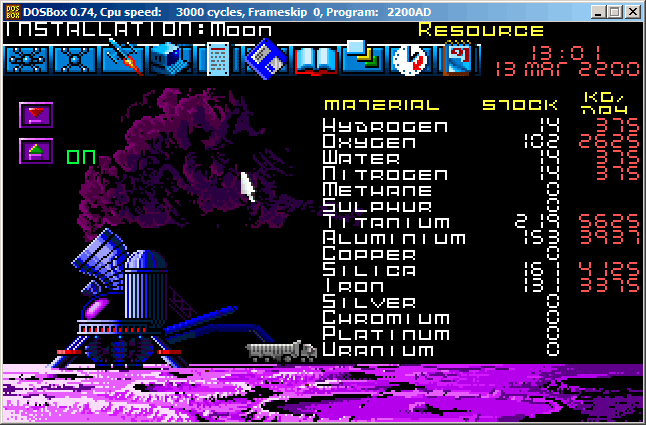
\includegraphics[scale=\FigScale]{ff/millenium/1.png}
\caption{\RU{Шахта: первое состояние}\EN{Mine: state 1}}
\label{fig:mill_1}
\end{figure}

\RU{Сохраним состояние игры}\EN{Let's save a game state}.
\RU{Это файл размером}\EN{This is a file of size} 9538 \RU{байт}\EN{bytes}.

\RU{Подождем несколько \q{дней} здесь в игре и теперь в шахте добыто больше ресурсов}%
\EN{Let's wait some \q{days} here in the game, and now we've got more resources from the mine}:

\begin{figure}[H]
\centering
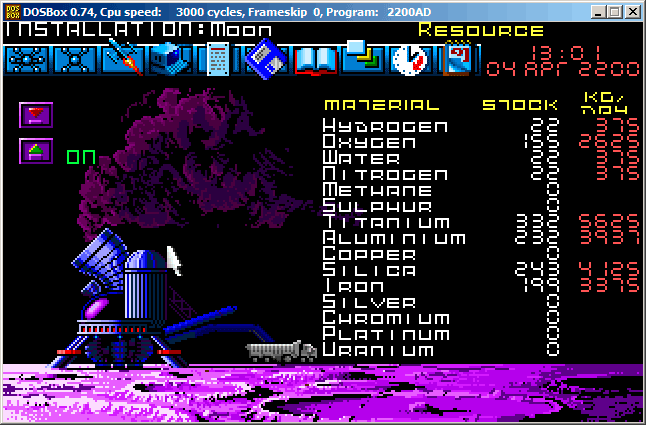
\includegraphics[scale=\FigScale]{ff/millenium/2.png}
\caption{\RU{Шахта: второе состояние}\EN{Mine: state 2}}
\label{fig:mill_2}
\end{figure}

\RU{Снова сохраним состояние игры}\EN{Let's sav game state again}.

\RU{Теперь просто попробуем сравнить оба файла побайтово используя простую утилиту FC под DOS/Windows:}
\EN{Now let's try to just do binary comparison of the save files using the simple DOS/Windows FC utility:}

\lstinputlisting{ff/millenium/fc_result.txt}

\RU{Вывод здесь неполный, там было больше отличий, но мы обрежем результат до самого интересного.}%
\EN{The output is incomplete here, there are more differences, but we will cut result to show the most interesting.}

\RU{В первой версии у нас было 14 единиц водорода (hydrogen) и 102 --- кислорода (oxygen).}
\EN{In the first state, we have 14 \q{units} of hydrogen and 102 \q{units} of oxygen.}
\RU{Во второй версии у нас 22 и 155 единиц соответственно.}
\EN{We have 22 and 155 \q{units} respectively in the second state.}
\RU{Если эти значения сохраняются в файл, мы должны увидеть разницу}\EN{If these values are saved into 
the save file, we would see this in the difference}.
\RU{И она действительно есть}\EN{And indeed we do}. 
\RU{Там}\EN{There is} 0x0E (14) \RU{на позиции}\EN{at position} 0xBDA \RU{и это значение}\EN{and this value is} 
0x16 (22) \RU{в новой версии файла}\EN{in the new version of the file}.
\RU{Это, наверное, водород}\EN{This is probably hydrogen}.
\RU{Там также}\EN{There is} 0x66 (102) \RU{на позиции}\EN{at position} 0xBDC \RU{в старой версии и}\EN{in the old 
version and} 0x9B (155) \RU{в новой версии файла}\EN{in the new version of the file}. 
\RU{Это, наверное, кислород}\EN{This seems to be the oxygen}.

\RU{Обе версии файла доступны на сайте, для тех кто хочет их изучить (или поэкспериментировать)}%
\EN{Both files are available on the website for those who wants to inspect them (or experiment) more}: 
\href{http://go.yurichev.com/17212}{beginners.re}.

\clearpage
\RU{Новую версию файла откроем в Hiew и отметим значения, связанные с ресурсами, добытыми на шахте в игре}%
\EN{Here is the new version of file opened in Hiew, we marked the values related to the resources mined in the game}: 

\begin{figure}[H]
\centering
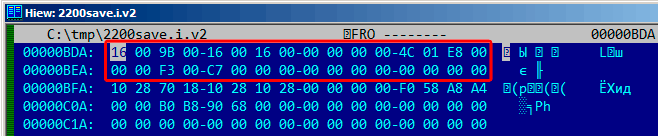
\includegraphics[scale=\FigScale]{ff/millenium/hiew3.png}
\caption{Hiew: \RU{первое состояние}\EN{state 1}}
\label{fig:mill_hiew3}
\end{figure}

\RU{Проверим каждое, и это они}\EN{Let's check each, and these are}.
\RU{Это явно 16-битные значения: не удивительно для 16-битной программы под DOS, где \Tint имел длину в 16 бит.}
\EN{These are clearly 16-bit values: not a strange thing for 16-bit DOS software where the \Tint type has 16-bit width.}

\clearpage
\RU{Проверим наши предположения}\EN{Let's check our assumptions}.
\RU{Запишем 1234 (0x4D2) на первой позиции (это должен быть водород)}%
\EN{We will write the 1234 (0x4D2) value at the first position (this must be hydrogen)}:

\begin{figure}[H]
\centering
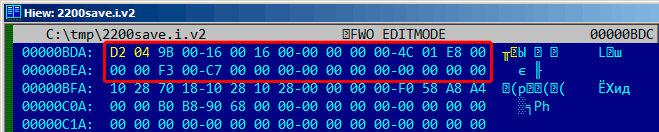
\includegraphics[scale=\FigScale]{ff/millenium/hiew4.png}
\caption{Hiew: \RU{запишем там}\EN{let's write 1234} (0x4D2)\EN{ there}}
\label{fig:mill_hiew4}
\end{figure}

\RU{Затем загрузим измененный файл в игру и посмотрим на статистику в шахте}%
\EN{Then we will load the changed file in the game and took a look at mine statistics}:

\begin{figure}[H]
\centering
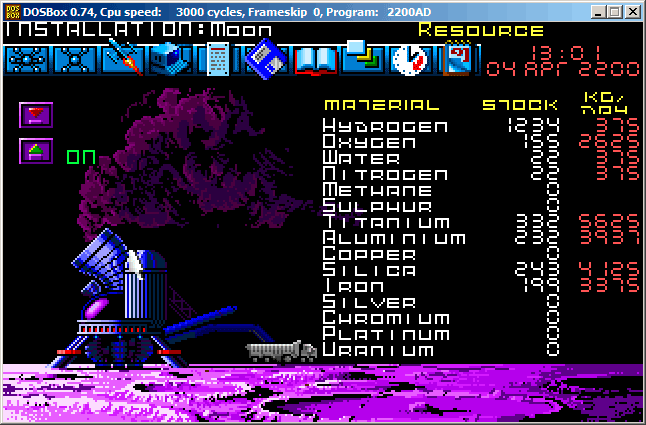
\includegraphics[scale=\FigScale]{ff/millenium/5.png}
\caption{\RU{Проверим значение водорода}\EN{Let's check for hydrogen value}}
\label{fig:mill_5}
\end{figure}

\RU{Так что да, это оно}\EN{So yes, this is it}.

\clearpage
\RU{Попробуем пройти игру как можно быстрее, установим максимальные значения везде}\EN{Now let's try to 
finish the game as soon as possible, set the maximal values everywhere}:

\begin{figure}[H]
\centering
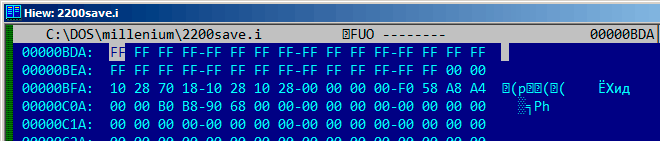
\includegraphics[scale=\FigScale]{ff/millenium/hiew7.png}
\caption{Hiew: \RU{установим максимальные значения}\EN{let's set maximal values}}
\label{fig:mill_hiew7}
\end{figure}

0xFFFF \RU{это}\EN{is} 65535, \RU{так что да, у нас много ресурсов теперь}\EN{so yes, we now have a 
lot of resources}:

\begin{figure}[H]
\centering
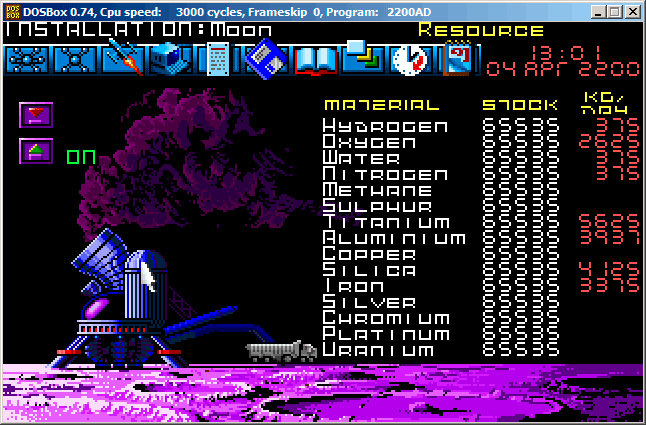
\includegraphics[scale=\FigScale]{ff/millenium/6.png}
\caption{\RU{Все ресурсы теперь действительно}\EN{All resources are} 65535 (0xFFFF)\EN{ indeed}}
\label{fig:mill_6}
\end{figure}

\clearpage
\RU{Пропустим еще несколько \q{дней} в игре и видим что-то неладное}\EN{Let's skip some \q{days} in the game and oops}! 
\RU{Некоторых ресурсов стало меньше}\EN{We have a lower amount of some resources}:

\begin{figure}[H]
\centering
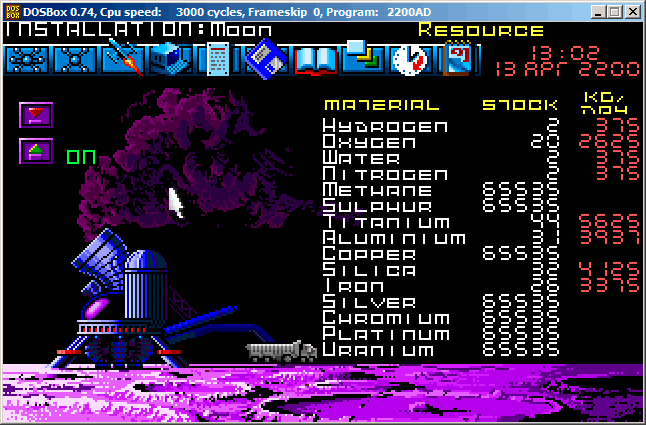
\includegraphics[scale=\FigScale]{ff/millenium/8.png}
\caption{\RU{Переполнение переменных ресурсов}\EN{Resource variables overflow}}
\label{fig:mill_8}
\end{figure}

\RU{Это просто переполнение}\EN{That's just overflow}. 
\RU{Разработчик игры вероятно никогда не думал, что значения ресурсов будут такими большими,
так что, здесь, наверное, нет проверок на переполнение, но шахта в игре \q{работает}, ресурсы добавляются,
отсюда и переполнение.}
\EN{The game's developer probably didn't think about such high amounts of resources,
so there are probably no overflow checks, but the mine is \q{working} in the game, resources are added,
hence the overflows.}
\RU{Вероятно, не нужно было жадничать}\EN{Apparently, it was a bad idea to be that greedy}.

\RU{Здесь наверняка еще какие-то значения в этом файле}\EN{There are probably a lot of more values 
saved in this file}.

\RU{Так что это очень простой способ читинга в играх}\EN{So this is very simple method of cheating in games}.
\RU{Файл с таблицей очков также можно легко модифицировать}\EN{High score files often can be easily 
patched like that}.

\EN{More about files and memory snapshots comparing}\RU{Еще насчет сравнения файлов и снимков памяти}: 
\myref{snapshots_comparing}.

\fi
\ifdefined\IncludeOracle
\chapter{\oracle: \EN{.SYM-files}\RU{.SYM-файлы}}
\index{\oracle}
\label{Oracle_SYM_files_example}

\RU{Когда процесс в \oracle терпит серьезную ошибку (crash), он записывает массу информации в лог-файлы,
включая состояние стека, вроде:}
\EN{When an \oracle process experiences some kind of crash, it writes a lot of information into log files,
including stack trace, like this:}

\begin{lstlisting}
----- Call Stack Trace -----
calling              call     entry                argument values in hex      
location             type     point                (? means dubious value)     
-------------------- -------- -------------------- ----------------------------
_kqvrow()                     00000000             
_opifch2()+2729      CALLptr  00000000             23D4B914 E47F264 1F19AE2
                                                   EB1C8A8 1
_kpoal8()+2832       CALLrel  _opifch2()           89 5 EB1CC74
_opiodr()+1248       CALLreg  00000000             5E 1C EB1F0A0
_ttcpip()+1051       CALLreg  00000000             5E 1C EB1F0A0 0
_opitsk()+1404       CALL???  00000000             C96C040 5E EB1F0A0 0 EB1ED30
                                                   EB1F1CC 53E52E 0 EB1F1F8
_opiino()+980        CALLrel  _opitsk()            0 0
_opiodr()+1248       CALLreg  00000000             3C 4 EB1FBF4
_opidrv()+1201       CALLrel  _opiodr()            3C 4 EB1FBF4 0
_sou2o()+55          CALLrel  _opidrv()            3C 4 EB1FBF4
_opimai_real()+124   CALLrel  _sou2o()             EB1FC04 3C 4 EB1FBF4
_opimai()+125        CALLrel  _opimai_real()       2 EB1FC2C
_OracleThreadStart@  CALLrel  _opimai()            2 EB1FF6C 7C88A7F4 EB1FC34 0
4()+830                                            EB1FD04
77E6481C             CALLreg  00000000             E41FF9C 0 0 E41FF9C 0 EB1FFC4
00000000             CALL???  00000000             
\end{lstlisting}

\RU{Но конечно, для этого исполняемые файлы \oracle должны содержать некоторую отладочную информацию,
либо map-файлы с информацией о символах или что-то в этом роде.}
\EN{But of course, \oracle's executables must have some kind of debug information or map files with symbol
information included or something like that.}

\RU{\oracle для Windows NT содержит информацию о символах в файлах с расширением .SYM, но его формат закрыт.}
\EN{Windows NT \oracle has symbol information in files with .SYM extension, but the format is proprietary.}
\EN{(Plain text files are good, but needs additional parsing, hence offer slower access.)}
\RU{(Простые текстовые файлы --- это хорошо, но они требуют дополнительной обработки (парсинга), и из-за этого доступ
к ним медленнее.)}

\RU{Посмотрим, сможем ли мы разобрать его формат}\EN{Let's see if we can understand its format}.
\RU{Выберем самый короткий файл \TT{orawtc8.sym}, поставляемый с файлом \TT{orawtc8.dll} в Oracle 8.1.7}%
\EN{We will pick the shortest \TT{orawtc8.sym} file that comes with the \TT{orawtc8.dll} file in Oracle 8.1.7}
\footnote{\RU{Будем использовать древнюю версию \oracle сознательно, из-за более короткого размера его модулей}%
\EN{We can chose an ancient \oracle version intentionally due to the smaller size of its modules}}.

\clearpage
\RU{Вот я открываю этот файл в}\EN{Here is the file opened in} Hiew:

\begin{figure}[H]
\centering
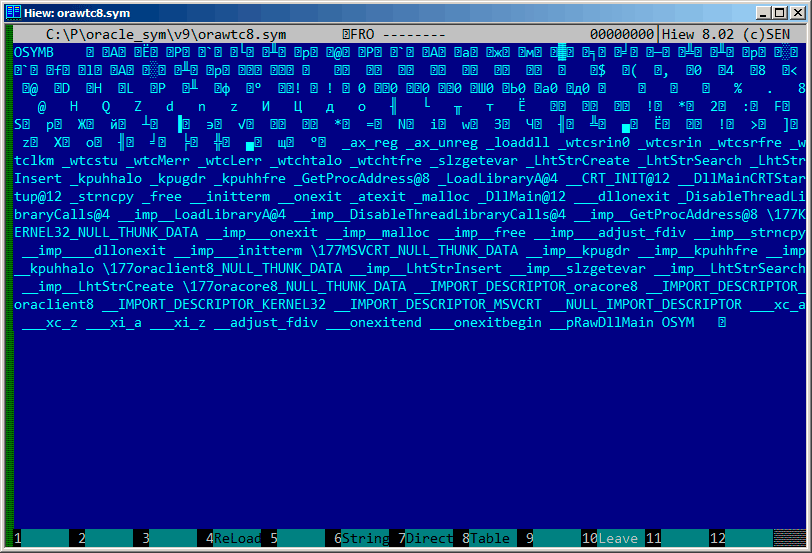
\includegraphics[scale=\FigScale]{ff/Oracle_SYM/whole1.png}
\caption{\RU{Весь файл в Hiew}\EN{The whole file in Hiew}}
\label{fig:oracle_SYM_whole1}
\end{figure}

\RU{Сравнивая этот файл с другими .SYM-файлами, мы можем быстро заметить, что \TT{OSYM} всегда является
заголовком (и концом), так что это, наверное, сигнатура файла.}
\EN{By comparing the file with other .SYM files, we can quickly see that \TT{OSYM} is always header (and footer),
so this is maybe the file's signature.}

\RU{Мы также видим, что в общем-то, формат файла это: OSYM + какие-то бинарные данные + 
текстовые строки разделенные нулем + OSYM.}
\EN{We also see that basically, the file format is: OSYM + some binary data + zero delimited text strings + OSYM.}
\RU{Строки --- это, очевидно, имена функций и глобальных переменных}\EN{The strings are, obviously, function and global 
variable names}.

\clearpage
\RU{Отметим сигнатуры OSYM и строки здесь}\EN{We will mark the OSYM signatures and strings here}: 

\begin{figure}[H]
\centering
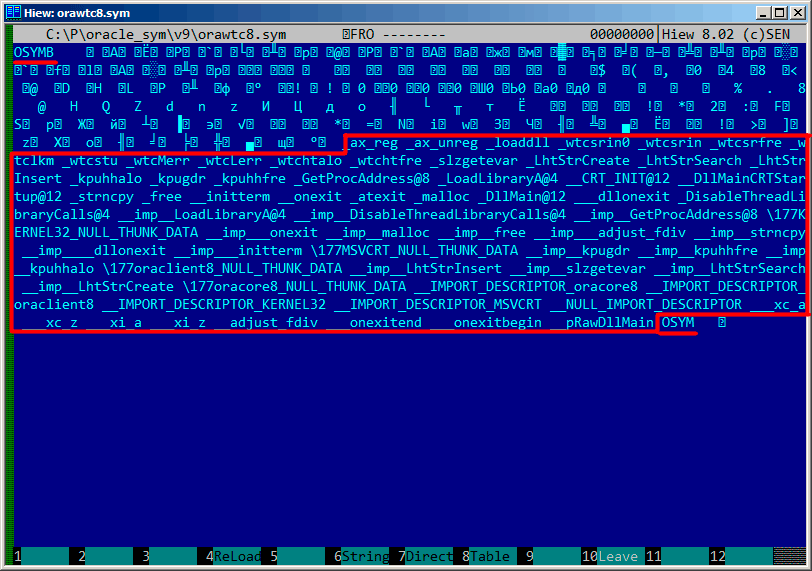
\includegraphics[scale=\FigScale]{ff/Oracle_SYM/whole2.png}
\caption{\RU{Сигнатура OSYM и текстовые строки}\EN{OSYM signature and text strings}}
\label{fig:oracle_SYM_whole2}
\end{figure}

\RU{Посмотрим}\EN{Well, let's see}. 
\RU{В Hiew отметим весь блок со строками (исключая оконечивающую сигнатуру OSYM) и сохраним его в отдельный
файл.}%
\EN{In Hiew, we will mark the whole strings block (except the trailing OSYM signatures) and put it into a separate file.}
\RU{Затем запустим UNIX-утилиты \IT{strings} и \IT{wc} для подсчета текстовых строк:}%
\EN{Then we run UNIX \IT{strings} and \IT{wc} utilities to count the text strings:}

\begin{lstlisting}
strings strings_block | wc -l
66
\end{lstlisting}

\RU{Так что здесь 66 текстовых строк}\EN{So there are 66 text strings}.
\RU{Запомните это число}\EN{Please note that number}.

\RU{Можно сказать, что в общем, как правило, количество \IT{чего-либо} часто сохраняется в бинарном
файле отдельно.}
\EN{We can say, in general, as a rule, the number of \IT{anything} is often stored separately in binary files.}
\RU{Это действительно так, мы можем найти значение 66 (0x42) в самом начале файла, прямо после сигнатуры OSYM:}
\EN{It's indeed so, we can find the 66 value (0x42) at the file's start, right after the OSYM signature:}

\lstinputlisting{ff/Oracle_SYM/dump1.txt}

\RU{Конечно, 0x42 здесь это не байт, но скорее всего, 32-битное значение, запакованное как little-endian,
поэтому мы видим 0x42 и затем как минимум 3 байта.}
\EN{Of course, 0x42 here is not a byte, but most likely a 32-bit value packed as little-endian, hence we see
0x42 and then at least 3 zero bytes.}

\RU{Почему мы полагаем, что оно 32-битное}\EN{Why do we believe it's 32-bit}?
\RU{Потому что файлы с символами в \oracle могут быть очень большими}\EN{Because, \oracle's symbol 
files may be pretty big}.
\RU{oracle.sym для главного исполняемого файла oracle.exe (версия 10.2.0.4) содержит \TT{0x3A38E} (238478) 
символов.}
\EN{The oracle.sym file for the main oracle.exe (version 10.2.0.4) executable contains \TT{0x3A38E} (238478) symbols.}
\RU{16-битного значения тут недостаточно}\EN{A 16-bit value isn't enough here}.

\RU{Проверим другие .SYM-файлы как этот и это подтвердит нашу догадку: значение после 32-битной сигнатуры OSYM
всегда отражает количество текстовых строк в файле.}%
\EN{We can check other .SYM files like this and it proves our guess: the value after the 32-bit OSYM signature always
reflects the number of text strings in the file.}

\RU{Это общая особенность почти всех бинарных файлов: заголовок с сигнатурой плюс некоторая дополнительная
информация о файле.}
\EN{It's a general feature of almost all binary files: a header with a signature plus some other information 
about the file.}

\RU{Рассмотрим бинарный блок поближе}\EN{Now let's investigate closer what this binary block is}.
\RU{Снова используя Hiew, сохраним блок начиная с адреса 8 (т.е. после 32-битного значения,
отражающего количество) до блока со строками, в отдельный файл.}%
\EN{Using Hiew again, we put the block starting at address 8 (i.e., after the 32-bit \IT{count} value) 
ending at the strings block, into a separate binary file.}

\clearpage
\RU{Посмотрим этот блок в}\EN{Let's see the binary block in} Hiew:

\begin{figure}[H]
\centering
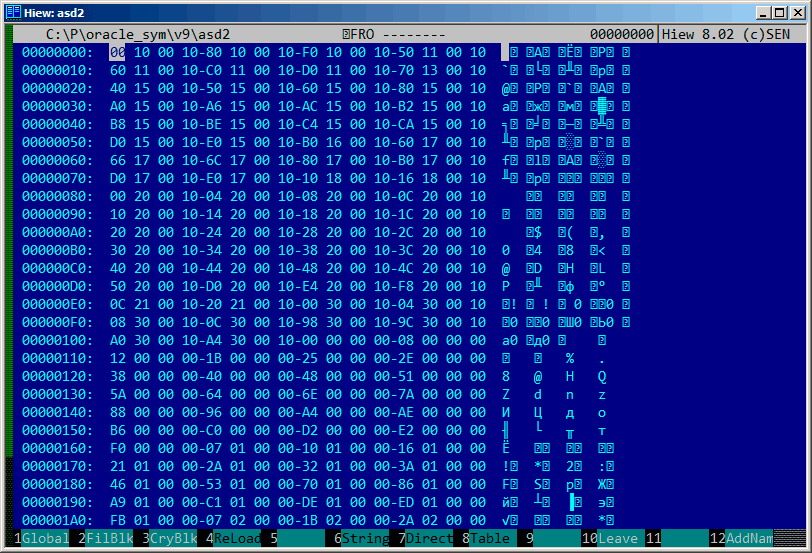
\includegraphics[scale=\FigScale]{ff/Oracle_SYM/binary1.png}
\caption{\RU{Бинарный блок}\EN{Binary block}}
\label{fig:oracle_SYM_binary1}
\end{figure}

\RU{Тут явно есть какая-то структура}\EN{There is a clear pattern in it}. 

\clearpage
\RU{Добавим красные линии, чтобы разделить блок}\EN{We will add red lines to divide the block}: 

\begin{figure}[H]
\centering
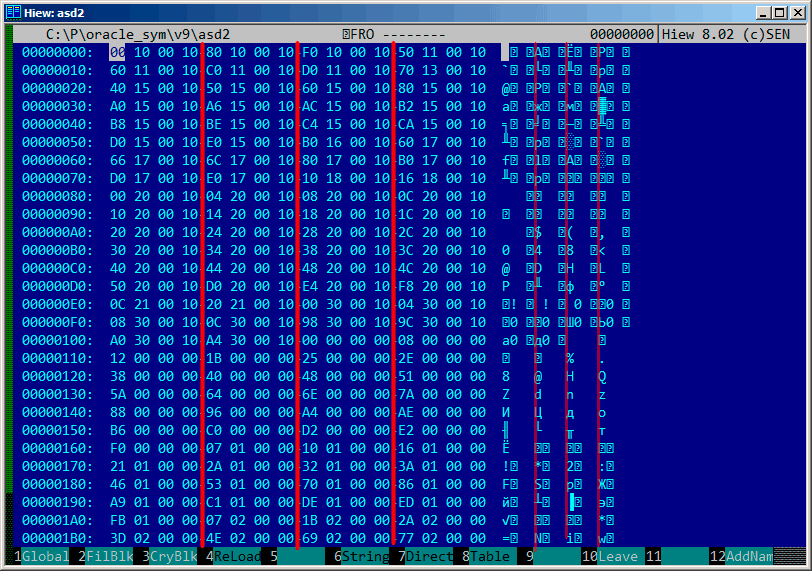
\includegraphics[scale=\FigScale]{ff/Oracle_SYM/binary2.png}
\caption{\RU{Структура бинарного блока}\EN{Binary block patterns}}
\label{fig:oracle_SYM_binary2}
\end{figure}

\RU{Hiew, как и многие другие шестнадцатеричные редакторы, показывает 16 байт на строку.}
\EN{Hiew, like almost any other hexadecimal editor, shows 16 bytes per line.}
\RU{Так что структура явно видна: здесь 4 32-битных значения на строку}\EN{So the pattern is clearly visible: 
there are 4 32-bit values per line}.

\RU{Эта структура видна визуально потому что некоторые значения здесь (вплоть до адреса \TT{0x104}) 
всегда в виде \TT{0x1000xxxx}, так что начинаются с байт 0x10 и 0.}
\EN{The pattern is visually visible because some values here (till address \TT{0x104}) 
are always in \TT{0x1000xxxx} form, 
started with 0x10 and zero bytes.}
\RU{Другие значения (начинающиеся на \TT{0x108}) всегда в виде \TT{0x0000xxxx}, так что начинаются с двух
нулевых байт.}
\EN{Other values (starting at \TT{0x108}) are in \TT{0x0000xxxx} form, so always started with two zero bytes.}

\RU{Посмотрим на этот блок как на массив 32-битных значений}\EN{Let's dump the block as an array of 32-bit values}:

\lstinputlisting[caption=\RU{первый столбец --- это адрес}\EN{first column is address}]{ff/Oracle_SYM/dump2.txt}

\RU{Здесь 132 значения, а это 66*2}\EN{There are 132 values, that's 66*2}.
\RU{Может быть здесь 2 32-битных значения на каждый символ, а может быть здесь два массива}\EN{Probably, 
there are two 32-bit values for each symbol, but maybe there are two arrays}? 
\RU{Посмотрим}\EN{Let's see}.

\RU{Значения, начинающиеся с}\EN{Values starting with} \TT{0x1000} \RU{могут быть адресами}\EN{may be addresses}.
\RU{В конце концов, этот .SYM-файл для DLL, а базовый адрес для DLL в win32 это \TT{0x10000000}, и сам код
обычно начинается по адресу \TT{0x10001000}.}
\EN{This is a .SYM file for a DLL after all, and the default base address of
win32 DLLs is \TT{0x10000000}, and the code usually starts at \TT{0x10001000}.}

\RU{Когда открываем файл orawtc8.dll в \IDA, базовый адрес другой, но тем не менее, первая функция это:}%
\EN{When we open the orawtc8.dll file in \IDA, the base address is different, but nevertheless, the first function is:}

\begin{lstlisting}
.text:60351000 sub_60351000    proc near
.text:60351000
.text:60351000 arg_0           = dword ptr  8
.text:60351000 arg_4           = dword ptr  0Ch
.text:60351000 arg_8           = dword ptr  10h
.text:60351000
.text:60351000                 push    ebp
.text:60351001                 mov     ebp, esp
.text:60351003                 mov     eax, dword_60353014
.text:60351008                 cmp     eax, 0FFFFFFFFh
.text:6035100B                 jnz     short loc_6035104F
.text:6035100D                 mov     ecx, hModule
.text:60351013                 xor     eax, eax
.text:60351015                 cmp     ecx, 0FFFFFFFFh
.text:60351018                 mov     dword_60353014, eax
.text:6035101D                 jnz     short loc_60351031
.text:6035101F                 call    sub_603510F0
.text:60351024                 mov     ecx, eax
.text:60351026                 mov     eax, dword_60353014
.text:6035102B                 mov     hModule, ecx
.text:60351031
.text:60351031 loc_60351031:                           ; CODE XREF: sub_60351000+1D
.text:60351031                 test    ecx, ecx
.text:60351033                 jbe     short loc_6035104F
.text:60351035                 push    offset ProcName ; "ax_reg"
.text:6035103A                 push    ecx             ; hModule
.text:6035103B                 call    ds:GetProcAddress
...
\end{lstlisting}

\RU{Ух ты}\EN{Wow}, \q{ax\_reg} \RU{звучит знакомо}\EN{string sounds familiar}. 
\RU{Действительно, это самая первая строка в блоке строк!}
\EN{It's indeed the first string in the strings block!}
\RU{Так что имя этой функции, похоже}\EN{So the name of this function seems to be} \q{ax\_reg}.

\RU{Вторая функция}\EN{The second function is}:

\begin{lstlisting}
.text:60351080 sub_60351080    proc near
.text:60351080
.text:60351080 arg_0           = dword ptr  8
.text:60351080 arg_4           = dword ptr  0Ch
.text:60351080
.text:60351080                 push    ebp
.text:60351081                 mov     ebp, esp
.text:60351083                 mov     eax, dword_60353018
.text:60351088                 cmp     eax, 0FFFFFFFFh
.text:6035108B                 jnz     short loc_603510CF
.text:6035108D                 mov     ecx, hModule
.text:60351093                 xor     eax, eax
.text:60351095                 cmp     ecx, 0FFFFFFFFh
.text:60351098                 mov     dword_60353018, eax
.text:6035109D                 jnz     short loc_603510B1
.text:6035109F                 call    sub_603510F0
.text:603510A4                 mov     ecx, eax
.text:603510A6                 mov     eax, dword_60353018
.text:603510AB                 mov     hModule, ecx
.text:603510B1
.text:603510B1 loc_603510B1:                           ; CODE XREF: sub_60351080+1D
.text:603510B1                 test    ecx, ecx
.text:603510B3                 jbe     short loc_603510CF
.text:603510B5                 push    offset aAx_unreg ; "ax_unreg"
.text:603510BA                 push    ecx             ; hModule
.text:603510BB                 call    ds:GetProcAddress
...
\end{lstlisting}

\RU{Строка \q{ax\_unreg} также это вторая строка в строке блок!}
\EN{The \q{ax\_unreg} string is also the second string in the strings block!}
\RU{Адрес начала второй функции это \TT{0x60351080}, а второе значение в бинарном блоке это \TT{10001080}.}
\EN{The starting address of the second function is \TT{0x60351080}, and the second value in the binary 
block is \TT{10001080}.}
\RU{Так что это адрес, но для DLL с базовым адресом по умолчанию}\EN{So this is the address, 
but for a DLL with the default base address}.

\RU{Мы можем быстро проверить и убедиться, что первые 66 значений в массиве (т.е. первая половина)
это просто адреса функций в DLL, включая некоторые метки, \etc{}.}
\EN{We can quickly check and be sure that the first 66 values in the array (i.e., the first half of the array) 
are just function addresses in the DLL, including some labels, \etc{}.}
\RU{Хорошо, что же тогда остальная часть массива}\EN{Well, what's the other part of array then}? 
\RU{Остальные 66 значений, начинающиеся с}\EN{The other 66 values that start with} \TT{0x0000}? 
\RU{Они похоже в пределах}\EN{These seem to be in range} \TT{[0...0x3F8]}. 
\RU{И не похоже, что это битовые поля: ряд чисел возрастает}\EN{And they do not look like bitfields: 
the series of numbers is increasing}.
\RU{Последняя шестнадцатеричная цифра выглядит как случайная, так что, не похоже, что это
адрес чего-либо (в противном случае, он бы делился, может быть, на 4 или 8 или 0x10).}
\EN{The last hexadecimal digit seems to be random, so, it's unlikely the address of something 
(it would be divisible by 4 or maybe 8 or 0x10 otherwise).}

\RU{Спросим себя: что еще разработчики \oracle хранили бы здесь, в этом файле?}
\EN{Let's ask ourselves: what else \oracle's developers would save here, in this file?}
\RU{Случайная догадка: это может быть адрес текстовой строки (название функции).}
\EN{Quick wild guess: it could be the address of the text string (function name).}
\RU{Это можно легко проверить, и да, каждое число --- это просто позиция первого символа в блоке строк.}
\EN{It can be quickly checked, and yes, each number is just the position of the first character in the strings block.}

\RU{Вот и всё! Всё закончено.}\EN{This is it! All done.}

\index{IDA}
\RU{Напишем утилиту для конвертирования .SYM-файлов в \IDA-скрипт, 
так что сможем загружать .idc-скрипт и он выставит имена функций:}%
\EN{We will write an utility to convert these .SYM files into \IDA script, 
so we can load the .idc script and it sets the function names:}

\lstinputlisting{ff/Oracle_SYM/unpacker.c}

\RU{Пример его работы}\EN{Here is an example of its work}:

\begin{lstlisting}
#include <idc.idc>

static main() {
	MakeName(0x60351000, "_ax_reg");
	MakeName(0x60351080, "_ax_unreg");
	MakeName(0x603510F0, "_loaddll");
	MakeName(0x60351150, "_wtcsrin0");
	MakeName(0x60351160, "_wtcsrin");
	MakeName(0x603511C0, "_wtcsrfre");
	MakeName(0x603511D0, "_wtclkm");
	MakeName(0x60351370, "_wtcstu");
...
}
\end{lstlisting}

\RU{Файлы, использованные в этом примере, здесь}\EN{The example files were used in this example are here}: 
\href{http://go.yurichev.com/17216}{beginners.re}.

\clearpage
\RU{О, можно еще попробовать \oracle для win64}\EN{Oh, let's also try \oracle for win64}.
\RU{Там ведь должны быть 64-битные адреса, верно}\EN{There has to be 64-bit addresses instead, right}?

\RU{8-байтная структура здесь видна даже еще лучше}\EN{The 8-byte pattern is visible even easier here}:

\begin{figure}[H]
\centering
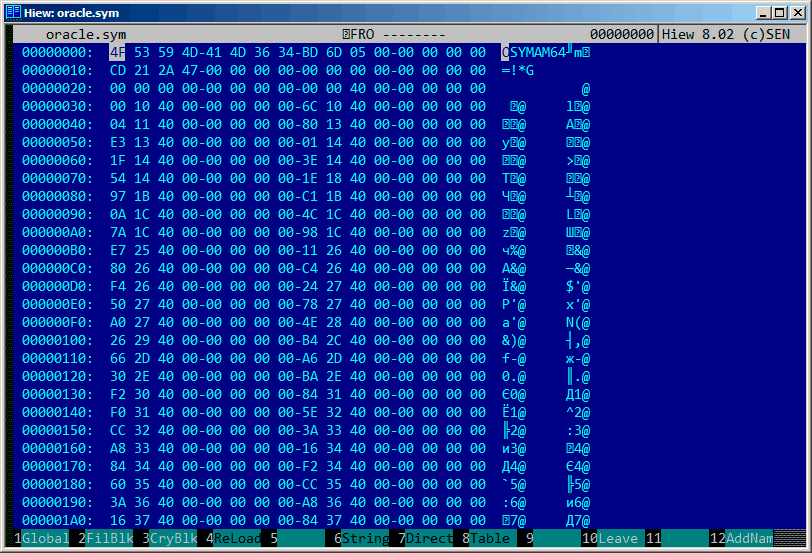
\includegraphics[scale=\FigScale]{ff/Oracle_SYM/whole64.png}
\caption{\RU{пример .SYM-файла из \oracle для win64}\EN{.SYM-file example from \oracle for win64}}
\label{fig:oracle_SYM_whole64}
\end{figure}

\RU{Так что да, все таблицы здесь имеют 64-битные элементы, даже смещения строк!}
\EN{So yes, all tables now have 64-bit elements, even string offsets!}
\RU{Сигнатура теперь \TT{OSYMAM64}, чтобы отличить целевую платформу, очевидно.}%
\EN{The signature is now \TT{OSYMAM64}, to distinguish the target platform, apparently.}

\RU{Вот и всё}\EN{This is it}!
\RU{Вот также библиотека в которой есть функция для доступа к .SYM-файлам \oracle}
\EN{Here is also library which has functions to access \oracle .SYM-files}:
\href{http://go.yurichev.com/17007}{GitHub}.

\chapter{\oracle: \EN{.MSB-files}\RU{.MSB-файлы}\ESph{}\PTBRph{}\PLph{}}
\index{\oracle}
\EN{\epigraph{When working toward the solution of a problem, it always helps if you know the answer.}{Murphy's Laws, Rule of Accuracy}}
\RU{\epigraph{Работая над решением задачи, всегда полезно знать ответ.}{Законы Мерфи, правило точности}}

\RU{Это бинарный файл, содержащий сообщения об ошибках вместе с их номерами.}
\EN{This is a binary file that contains error messages with their corresponding numbers.}
\RU{Давайте попробуем понять его формат и найти способ распаковать его}\EN{Let's try to understand 
its format and find a way to unpack it}.

\RU{В \oracle имеются файлы с сообщениями об ошибках в текстовом виде, так что мы можем сравнивать файлы:
текстовый и запакованный бинарный}\EN{There are \oracle error message files in text form, 
so we can compare the text and packed binary files}
\footnote{\EN{Open-source text files don't exist in \oracle for every .MSB file, so that's why we will work on their file format}
\RU{Текстовые файлы с открытым кодом в \oracle имеются не для каждого .MSB-файла, вот почему мы будем работать над его форматом}}.

\RU{Это начало файла}\EN{This is the beginning of the} ORAUS.MSG \RU{без ненужных комментариев}\EN{text file 
with some irrelevant comments stripped}:

\begin{lstlisting}[caption=\RU{Начало файла}\EN{Beginning of} ORAUS.MSG \RU{без комментариев}\EN{file without comments}]
00000, 00000, "normal, successful completion"
00001, 00000, "unique constraint (%s.%s) violated"
00017, 00000, "session requested to set trace event"
00018, 00000, "maximum number of sessions exceeded"
00019, 00000, "maximum number of session licenses exceeded"
00020, 00000, "maximum number of processes (%s) exceeded"
00021, 00000, "session attached to some other process; cannot switch session"
00022, 00000, "invalid session ID; access denied"
00023, 00000, "session references process private memory; cannot detach session"
00024, 00000, "logins from more than one process not allowed in single-process mode"
00025, 00000, "failed to allocate %s"
00026, 00000, "missing or invalid session ID"
00027, 00000, "cannot kill current session"
00028, 00000, "your session has been killed"
00029, 00000, "session is not a user session"
00030, 00000, "User session ID does not exist."
00031, 00000, "session marked for kill"
...
\end{lstlisting}

\RU{Первое число\EMDASH{}это код ошибки}\EN{The first number is the error code}.
\RU{Второе это, вероятно, могут быть дополнительные флаги}\EN{The second is perhaps maybe some additional flags}.

\clearpage
\RU{Давайте откроем бинарный файл}\EN{Now let's open the} ORAUS.MSB 
\RU{и найдем эти текстовые строки}\EN{binary file and find these text strings}. 
\RU{И вот они}\EN{And there are}:

\begin{figure}[H]
\centering
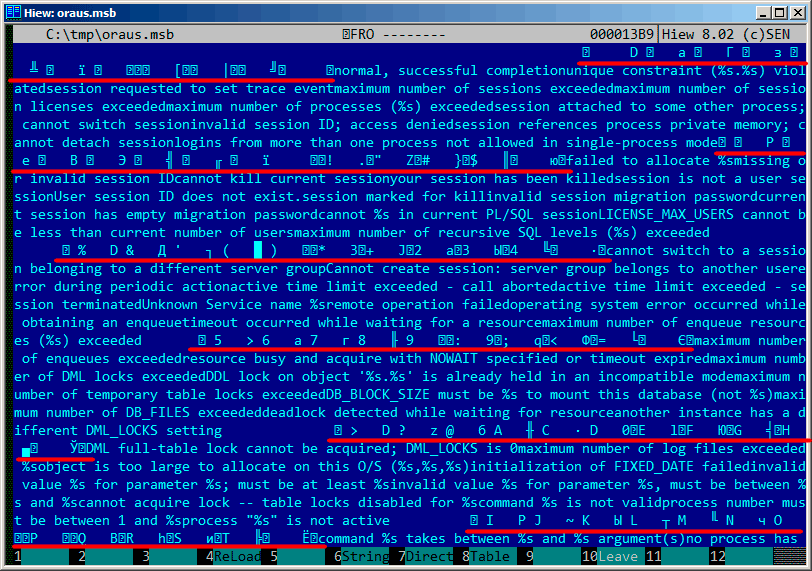
\includegraphics[scale=\FigScale]{ff/Oracle_MSB/1.png}
\caption{Hiew: \RU{первый блок}\EN{first block}}
\label{fig:oracle_MSB_1}
\end{figure}

\RU{Мы видим текстовые строки (включая те, с которых начинается файл ORAUS.MSG) перемежаемые с какими-то
бинарными значениями}\EN{We see the text strings (including those from the beginning of the ORAUS.MSG file) 
interleaved with some binary values}.
\RU{Мы можем довольно быстро обнаружить что главная часть бинарного файла поделена на блоки размером 0x200 (512)
байт}\EN{By quick investigation, we can see that main part of the binary file is divided by blocks of 
size 0x200 (512) bytes}.

\clearpage
\RU{Посмотрим содержимое первого блока}\EN{Let's see the contents of the first block}:

\begin{figure}[H]
\centering
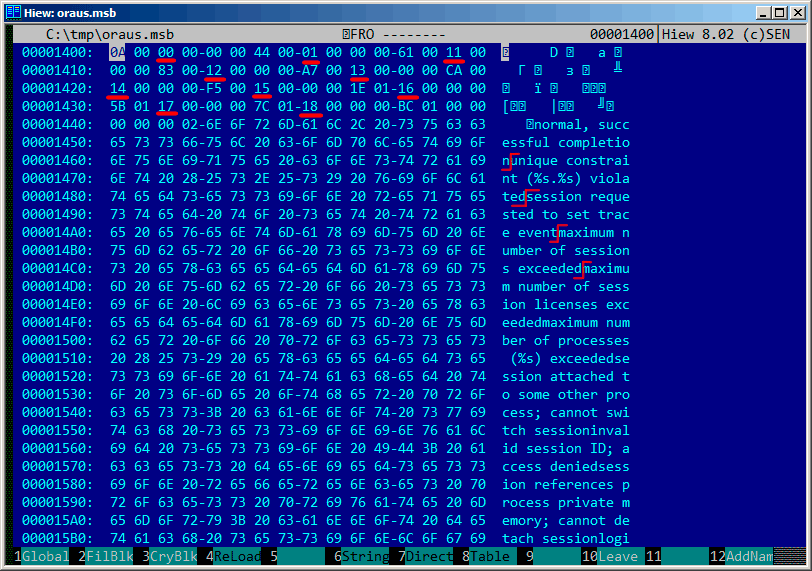
\includegraphics[scale=\FigScale]{ff/Oracle_MSB/2.png}
\caption{Hiew: \RU{первый блок}\EN{first block}}
\label{fig:oracle_MSB_2}
\end{figure}

\RU{Мы видим тексты первых сообщений об ошибках}\EN{Here we see the texts of the first messages errors}.
\RU{Что мы видим еще, так это то, что здесь нет нулевых байтов между сообщениями}\EN{What we also see is 
that there are no zero bytes between the error messages}.
\RU{Это значит, что это не оканчивающиеся нулем Си-строки}\EN{This implies that these are not null-terminated C strings}.
\RU{Как следствие, длина каждого сообщения об ошибке должна быть как-то закодирована}\EN{As a consequence, 
the length of each error message must be encoded somehow}.
\RU{Попробуем также найти номера ошибок}\EN{Let's also try to find the error numbers}.
\RU{Файл}\EN{The} ORAUS.MSG \RU{начинается с таких}\EN{files starts with these}: 
0, 1, 17 (0x11), 18 (0x12), 19 (0x13), 20 (0x14), 21 (0x15), 22 (0x16), 23 (0x17), 24 (0x18)...
\RU{Найдем эти числа в начале блока и отметим их красными линиями}\EN{We will find these numbers in the beginning 
of the block and mark them with red lines}.
\RU{Период между кодами ошибок 6 байт}\EN{The period between error codes is 6 bytes}.
\RU{Это значит, здесь, наверное, 6 байт информации выделено для каждого сообщения об ошибке.}
\EN{This implies that there are probably 6 bytes of information allocated for each error message.}

\RU{Первое 16-битное значение (здесь 0xA или 10) означает количество сообщений в блоке: это можно проверить глядя на другие блоки.}%
\EN{The first 16-bit value (0xA here or 10) mean the number of messages in each block: this can be checked by investigating other blocks.}
\RU{Действительно: сообщения об ошибках имеют произвольный размер}\EN{Indeed: the error messages have arbitrary size}. 
\RU{Некоторые длиннее, некоторые короче}\EN{Some are longer, some are shorter}. 
\RU{Но длина блока всегда фиксирована, следовательно, никогда не знаешь, сколько сообщений можно запаковать
в каждый блок}\EN{But block size is always fixed, hence,
you never know how many text messages can be packed in each block}.

\RU{Как мы уже отметили, так как это не оканчивающиеся нулем Си-строки, длина строки должна быть закодирована где-то.}%
\EN{As we already noted, since these are not null-terminating C strings, their size must be encoded somewhere.}
\RU{Длина первой строки}\EN{The size of the first string} \q{normal, successful completion} \RU{это}\EN{is} 
29 (0x1D) \RU{байт}\EN{bytes}.
\RU{Длина второй строки}\EN{The size of the second string} \q{unique constraint (\%s.\%s) violated} 
\RU{это}\EN{is} 34 (0x22) \RU{байт}\EN{bytes}.
\RU{Мы не можем отыскать этих значений}\EN{We can't find these values} (0x1D \OrENRU/\AndENRU 0x22) 
\RU{в блоке}\EN{in the block}.

\RU{А вот еще кое-что}\EN{There is also another thing}.
\oracle \RU{должен как-то определять позицию строки, которую он должен загрузить, верно}
\EN{has to determine the position of the string it needs to load in the block, right}?
\RU{Первая строка}\EN{The first string} \q{normal, successful completion} \RU{начинается с позиции}\EN{starts 
at  position} 0x1444 (\RU{если считать с начала бинарного файла}\EN{if we count starting at the beginning of the file}) \RU{или с}\EN{or at} 0x44 (\RU{от начала блока}\EN{from the block's start}).
\RU{Вторая строка}\EN{The second string} \q{unique constraint (\%s.\%s) violated} 
\RU{начинается с позиции}\EN{starts at position} 0x1461 (\RU{от начала файла}\EN{from the
file's start}) \RU{или с}\EN{or at} 0x61 (\RU{считая с начала блока}\EN{from the at the block's start}).
\RU{Эти числа}\EN{These numbers} (0x44 \AndENRU 0x61) \RU{нам знакомы}\EN{are familiar somehow}! 
\RU{Мы их можем легко отыскать в начале блока}\EN{We can clearly see them at the start of the block}.

\RU{Так что, каждый 6-байтный блок это}\EN{So, each 6-byte block is}:

\begin{itemize}
\item 16-\RU{битный номер ошибки}\EN{bit error number}; 
\item 16-\RU{битный ноль (может быть, дополнительные флаги}\EN{bit zero (maybe additional flags)}; 
\item 16-\RU{битная начальная позиция текстовой строки внутри текущего блока}\EN{bit starting position of 
the text string within the current block}.
\end{itemize}

\RU{Мы можем быстро проверить остальные значения чтобы удостовериться в своей правоте}%
\EN{We can quickly check the other values and be sure our guess is correct}.
\RU{И здесь еще последний \q{пустой} 6-байтный блок с нулевым номером ошибки и начальной позицией за последним
символом последнего сообщения об ошибке.}\EN{And there is also the last \q{dummy} 6-byte block 
with an error number of zero and starting position beyond the last error message's last character.}
\RU{Может быть именно так и определяется длина сообщения}\EN{Probably that's how text message length is 
determined}?
\RU{Мы просто перебираем 6-байтные блоки в поисках нужного номера ошибки, затем
мы узнаем позицию текстовой строки, затем мы узнаем позицию следующей текстовой строки глядя на
следующий 6-байтный блок!}\EN{We just enumerate 6-byte blocks to find the error number
we need, then we get the text string's position, then we get the position of the text string by looking at the next
6-byte block!}
\RU{Так мы определяем границы строки}\EN{This way we determine the string's boundaries}!
\RU{Этот метод позволяет сэкономить место в файле не записывая длину строки}\EN{This method allows to 
save some space by not saving the text string's size in the file}!
\RU{Нельзя сказать, что экономия памяти большая, но это интересный трюк.}%
\EN{It's not possible to say it saves a lot of space, but it's a clever trick}.

\clearpage
\RU{Вернемся к заголовку .MSB-файла}\EN{Let's back to the header of .MSB-file}:

\begin{figure}[H]
\centering
\includegraphics[scale=\FigScale]{ff/Oracle_MSB/3.png}
\caption{Hiew: \RU{заголовок файла}\EN{file header}}
\label{fig:oracle_MSB_3}
\end{figure}

\RU{Теперь мы можем быстро найти количество блоков (отмечено красным)}\EN{Now we can quickly find the number of blocks in the file 
(marked by red)}.
\RU{Проверяем другие .MSB-файлы и оказывается что это справедливо для всех}\EN{We can checked other .MSB-files and we see that it's true 
for all of them}.
\RU{Здесь есть много других значений, но мы не будем разбираться с ними, так как наша задача (утилита для распаковки) уже решена.}
\EN{There are a lot of other values, but we will not investigate them, since our job (an unpacking utility) was done.}
\RU{А если бы мы писали запаковщик .MSB-файлов, тогда нам наверное пришлось бы понять, зачем нужны остальные.}
\EN{If we have to write a .MSB file packer, we would probably need to understand the meaning of the other values.}

\clearpage
\RU{Тут еще есть таблица после заголовка, вероятно, содержащая 16-битные значения}\EN{There is also a 
table that came after the header which probably contains 16-bit values}:

\begin{figure}[H]
\centering
\includegraphics[scale=\FigScale]{ff/Oracle_MSB/4.png}
\caption{Hiew: \RU{таблица }last\_errnos\EN{ table}}
\label{fig:oracle_MSB_4}
\end{figure}

\RU{Их длина может быть определена визуально (здесь нарисованы красные линии).}%
\EN{Their size can be determined visually (red lines are drawn here).}
\RU{Когда мы сдампили эти значения, мы обнаружили, что каждое 16-битное число\EMDASH{}это последний код ошибки для каждого блока.}%
\EN{While dumping these values, we have found that each 16-bit number is the last error code for each block.}

\RU{Так вот как \oracle быстро находит сообщение об ошибке}\EN{So that's how \oracle quickly finds the error message}:

\begin{itemize}
\item \RU{загружает таблицу, которую мы назовем}\EN{load a table we will call} last\_errnos 
(\RU{содержащую последний номер ошибки для каждого блока}\EN{that contains the last error number for each block});
\item \RU{находит блок содержащий код ошибки, полагая что все коды ошибок увеличиваются и внутри каждого блока
и также в файле}\EN{find a block that contains the error code we need, assuming all error codes 
increase across each block and across the file as well};
\item \RU{загружает соответствующий блок}\EN{load the specific block};
\item \RU{перебирает 6-байтные структуры, пока не найдется соответствующий номер ошибки}\EN{enumerate the 6-byte 
structures until the specific error number is found};
\item \RU{находит позицию первого символа из текущего 6-байтного блока}\EN{get the position of the first 
character from the current 6-byte block};
\item \RU{находит позицию последнего символа из следующего 6-байтного блока}\EN{get the position of the last 
character from the next 6-byte block};
\item \RU{загружает все символы сообщения в этих пределах}\EN{load all characters of the message in this range}.
\end{itemize}

\RU{Это программа на Си которую мы написали для распаковки .MSB-файлов}
\EN{This is C program that we wrote which unpacks .MSB-files}:
\href{http://go.yurichev.com/17213}{beginners.re}.

\RU{И еще два файла которые были использованы в этом примере}
\EN{There are also the two files which were used in the example} 
(\oracle 11.1.0.6):
\href{http://go.yurichev.com/17214}{beginners.re},
\href{http://go.yurichev.com/17215}{beginners.re}.

\section{\RU{Вывод}\EN{Summary}}

\RU{Этот метод, наверное, слишком олд-скульный для современных компьютеров}\EN{The method is probably too 
old-school for modern computers}.
\RU{Возможно, формат этого файла был разработан в середине 1980-х кем-то, кто программировал для мейнфреймов,
учитывая экономию памяти и места на дисках}\EN{Supposedly, this file format was developed in the mid-80's by 
someone who also coded for \IT{big iron} with
memory/disk space economy in mind}.
\RU{Тем не менее, это интересная (хотя и простая) задача на разбор проприетарного формата файла без
заглядывания в код \oracle}\EN{Nevertheless, it was an interesting and yet easy task 
to understand a proprietary file format without looking into \oracle's code}.

\fi

% another place for `unsorted' sections

\part{\RU{Прочее}\EN{Other things}}

\chapter{npad}
\label{sec:npad}

\RU{Это макрос в ассемблере, для выравнивания некоторой метки по некоторой границе.}
\EN{It is an assembly language macro for aligning labels on a specific boundary.}

\RU{Это нужно для тех \IT{нагруженных} меток, куда чаще всего передается управление, например, 
начало тела цикла. 
Для того чтобы процессор мог эффективнее вытягивать данные или код из памяти, через шину с памятью, 
кэширование,\etc{}.}
\EN{That's often needed for the busy labels to where the control flow is often passed, e.g., loop body starts.
So the CPU can load the data or code from the memory effectively, through the memory bus, cache lines, \etc{}.}

\RU{Взято из}\EN{Taken from} \TT{listing.inc} (MSVC):

\index{x86!\Instructions!NOP}
\RU{Это, кстати, любопытный пример различных вариантов \NOP{}-ов. 
Все эти инструкции не дают никакого эффекта, но отличаются разной длиной.}
\EN{By the way, it is a curious example of the different \NOP variations.
All these instructions have no effects whatsoever, but have a different size.}

\RU{Цель в том, чтобы была только одна инструкция, а не набор NOP-ов, 
считается что так лучше для производительности CPU.}
\EN{Having a single idle instruction instead of couple of NOP-s,
is accepted to be better for CPU performance.}

\begin{lstlisting}
;; LISTING.INC
;;
;; This file contains assembler macros and is included by the files created
;; with the -FA compiler switch to be assembled by MASM (Microsoft Macro
;; Assembler).
;;
;; Copyright (c) 1993-2003, Microsoft Corporation. All rights reserved.

;; non destructive nops
npad macro size
if size eq 1
  nop
else
 if size eq 2
   mov edi, edi
 else
  if size eq 3
    ; lea ecx, [ecx+00]
    DB 8DH, 49H, 00H
  else
   if size eq 4
     ; lea esp, [esp+00]
     DB 8DH, 64H, 24H, 00H
   else
    if size eq 5
      add eax, DWORD PTR 0
    else
     if size eq 6
       ; lea ebx, [ebx+00000000]
       DB 8DH, 9BH, 00H, 00H, 00H, 00H
     else
      if size eq 7
	; lea esp, [esp+00000000]
	DB 8DH, 0A4H, 24H, 00H, 00H, 00H, 00H 
      else
       if size eq 8
        ; jmp .+8; .npad 6
	DB 0EBH, 06H, 8DH, 9BH, 00H, 00H, 00H, 00H
       else
        if size eq 9
         ; jmp .+9; .npad 7
         DB 0EBH, 07H, 8DH, 0A4H, 24H, 00H, 00H, 00H, 00H
        else
         if size eq 10
          ; jmp .+A; .npad 7; .npad 1
          DB 0EBH, 08H, 8DH, 0A4H, 24H, 00H, 00H, 00H, 00H, 90H
         else
          if size eq 11
           ; jmp .+B; .npad 7; .npad 2
           DB 0EBH, 09H, 8DH, 0A4H, 24H, 00H, 00H, 00H, 00H, 8BH, 0FFH
          else
           if size eq 12
            ; jmp .+C; .npad 7; .npad 3
            DB 0EBH, 0AH, 8DH, 0A4H, 24H, 00H, 00H, 00H, 00H, 8DH, 49H, 00H
           else
            if size eq 13
             ; jmp .+D; .npad 7; .npad 4
             DB 0EBH, 0BH, 8DH, 0A4H, 24H, 00H, 00H, 00H, 00H, 8DH, 64H, 24H, 00H
            else
             if size eq 14
              ; jmp .+E; .npad 7; .npad 5
              DB 0EBH, 0CH, 8DH, 0A4H, 24H, 00H, 00H, 00H, 00H, 05H, 00H, 00H, 00H, 00H
             else
              if size eq 15
               ; jmp .+F; .npad 7; .npad 6
               DB 0EBH, 0DH, 8DH, 0A4H, 24H, 00H, 00H, 00H, 00H, 8DH, 9BH, 00H, 00H, 00H, 00H
              else
	       %out error: unsupported npad size
               .err
              endif
             endif
            endif
           endif
          endif
         endif
        endif
       endif
      endif
     endif
    endif
   endif
  endif
 endif
endif
endm
\end{lstlisting}

\chapter{\RU{Модификация исполняемых файлов}\EN{Executable files patching}}

\section{\RU{Текстовые строки}\EN{Text strings}}

\RU{Сишные строки проще всего модифицировать (если они не зашифрованы) в любом шестнадцатеричном редакторе}
\EN{The C strings are the thing that is the easiest to patch (unless they are encrypted) in any hex editor}.
\RU{Эта техника доступна даже для тех, кто вовсе не разбирается в машинном коде и форматах исполняемых
файлов}\EN{This technique is available even for those who are not aware of machine code and executable file formats}.
\RU{Новая строка не должна быть длиннее старой, потому что имеется риск затереть какую-то другую переменную
или код}\EN{The new string has not to be bigger than the old one, because there's a risk of overwriting another value or code
there}.
\index{MS-DOS}
\RU{Используя этот метод, очень много ПО было \IT{локализовано} во времена MS-DOS, как минимум,
в странах бывшего СССР, в 80-х и 90-х}
\EN{Using this method, a lot of software was \IT{localized} in the MS-DOS era, at least in the ex-USSR countries in 80's
and 90's}.
\RU{Отсюда наличие очень странных аббревиатур и сокращений в \IT{локализованном} ПО: 
там просто не было места для более
длинных строк}\EN{It was the reason why some weird abbreviations were present in the \IT{localized} software: there was no room for
longer strings}.

\index{Borland Delphi}
\RU{В строках в Delphi, длина строки также должна быть поправлена, если нужно}
\EN{As for Delphi strings, the string's size must also be corrected, if needed}.

\section{x86\RU{-код}\EN{ code}}
\label{x86_patching}

\RU{Часто необходимые задачи}\EN{Frequent patching tasks are}:

\begin{itemize}

\index{x86!\Instructions!NOP}
\item \RU{Часто нужно просто запретить исполнение какой-либо инструкции}
\EN{One of the most frequent jobs is to disable some instruction}.
\RU{И чаще всего, это можно сделать, заполняя её байтом}\EN{It is often done by filling it using byte} 
\TT{0x90} (\ac{NOP}).

\item \RU{Условные переходы, имеющие опкод вроде}\EN{Conditional jumps, which have an opcode like} \TT{74 xx} (\JZ), 
\RU{так же могут быть заполнены двумя \ac{NOP}-ами}\EN{can be filled with two \ac{NOP}s}.
\RU{Также возможно запретить исполнение условного перехода записав 0 во второй байт}
\EN{It is also possible to disable a conditional jump by writing 0 at the second byte} (\IT{jump offset}).

\index{x86!\Instructions!JMP}
\item \RU{Еще одна часто необходимая задача это сделать условный переход всегда срабатывающим}
\EN{Another frequent job is to make a conditional jump to always trigger}: 
\RU{это возможно при помощи записи}\EN{this can be done by writing} \TT{0xEB} 
\RU{вместо опкода, это значит}
\EN{instead of the opcode, which stands for} \JMP.

\index{x86!\Instructions!RET}
\index{stdcall}
\item \RU{Исполнение функции может быть запрещено, если записать}\EN{A function's execution can be disabled by writing}
\RETN (0xC3) \RU{в её начале}\EN{at its beginning}.
\RU{Это справедливо для всех функций кроме}\EN{This is true for all functions excluding} \TT{stdcall} 
(\myref{sec:stdcall}).
\RU{При модификации функций}\EN{While patching} \TT{stdcall}\RU{, нужно в начале определить количество аргументов 
(например, отыскав \RETN в этой функции),
и использовать}\EN{ functions, one has to determine the number of arguments (for example, 
by finding \RETN in this function), 
and use} \RETN \RU{с 16-битным аргументом}\EN{with a 16-bit argument} (0xC2).

\index{x86!\Instructions!MOV}
\index{x86!\Instructions!XOR}
\index{x86!\Instructions!INC}
\item \RU{Иногда, запрещенная функция должна возвращать}\EN{Sometimes, a disabled functions has to return} 0 \OrENRU 1.
\RU{Это можно сделать при помощи}\EN{This can be done by} \TT{MOV EAX, 0} \OrENRU \TT{MOV EAX, 1}, 
\RU{но это слишком многословно}\EN{but it's slightly verbose}.
\RU{Способ получше это}\EN{A better way is} \TT{XOR EAX, EAX} (2 \RU{байта}\EN{bytes} \TT{0x31 0xC0}) 
\OrENRU 
\TT{XOR EAX, EAX / INC EAX} (3 \RU{байта}\EN{bytes} \TT{0x31 0xC0 0x40}).

\end{itemize}

\RU{ПО может быть защищено от модификаций}\EN{A software may be protected against modifications}.
\RU{Эта защита чаще всего реализуется путем чтения кода и вычисления контрольной суммы}
\EN{This protection is often done by reading the executable code and calculating a checksum}.
\RU{Следовательно, код должен быть прочитан перед тем как защита сработает}\EN{Therefore, 
the code must be read before protection is triggered}.
\RU{Это можно определить установив точку останова на чтение памяти}
\EN{This can be determined by setting a breakpoint on reading memory}.

\index{tracer}
\RU{В \tracer имеется опция BPM для этого}\EN{\tracer has the BPM option for this}.

\RU{Релоки в исполняемых PE-файлах}\EN{PE executable file relocs} (\myref{subsec:relocs}) 
\RU{не должны быть тронуты, потому что загрузчик Windows перезапишет ваш новый код.}
\EN{must not to be touched while patching, 
because the Windows loader may overwrite your new code.}
\index{Hiew}
(\RU{Они выделяются серым в Hiew, например}\EN{They are grayed in Hiew, for example}:
\figref{fig:scanf_ex3_hiew_1}).
\RU{В качестве последней меры, можно записать \JMP для обхода релока, либо же придется модифицировать таблицу
релоков.}
\EN{As a last resort, it is possible to write jumps that circumvent the relocs, 
or you will need to edit the relocs table.}


\chapter{Compiler intrinsic}
\index{Compiler intrinsic}
\label{sec:compiler_intrinsic}

\index{x86!\Instructions!ROL}
\index{x86!\Instructions!ROR}
\RU{Специфичная для компилятора функция не являющаяся обычной библиотечной функцией.
Компилятор вместо её вызова генерирует определенный машинный код.
Нередко, это псевдофункции для определенной инструкции \ac{CPU}. \\
\\
Например, в языках \CCpp нет операции циклического сдвига, а во многих \ac{CPU} она есть.
Чтобы программисту были доступны эти инструкции, в MSVC есть псевдофункции 
\IT{\_rotl()} \AndENRU \IT{\_rotr()}\FNMSDNROTxURL{},
которые компилятором напрямую транслируются в x86-инструкции \TT{ROL}/\TT{ROR}. \\
\\
Еще один пример это функции позволяющие генерировать SSE-инструкции прямо в коде.}
\EN{A function specific to a compiler which is not an usual library function.
The compiler generates a specific machine code instead of a call to it.
It is often a pseudofunction for specific \ac{CPU} instruction. \\
\\
For example, there are no cyclic shift operations in \CCpp languages, but they are present in most \ac{CPU}s.
For programmer's convenience, at least MSVC has pseudofunctions
\IT{\_rotl()} \AndENRU \IT{\_rotr()}\FNMSDNROTxURL{}
which are translated by the compiler directly to the ROL/ROR x86 instructions. \\
\\
Another example are functions to generate SSE-instructions right in the code.}

\RU{Полный список intrinsics от MSVC}\EN{Full list of MSVC intrinsics}:
\href{http://go.yurichev.com/17254}{MSDN}.


\chapter{\RU{Аномалии компиляторов}\EN{Compiler's anomalies}}
\label{anomaly:Intel}
\index{\CompilerAnomaly}
\index{Intel C++}
\index{\oracle}
\index{x86!\Instructions!JZ}

\RU{Intel C++ 10.1 которым скомпилирован \oracle 11.2 Linux86, может сгенерировать два \JZ идущих подряд, 
причем на второй \JZ нет ссылки ниоткуда. Второй \JZ таким образом, не имеет никакого смысла.}
\EN{Intel C++ 10.1, which was used for \oracle 11.2 Linux86 compilation, may emit two \JZ in row,
and there are no references to the second \JZ. The second \JZ is thus meaningless.}

\begin{lstlisting}[caption=\RU{kdli.o из}\EN{kdli.o from} libserver11.a]
.text:08114CF1                   loc_8114CF1: ; CODE XREF: __PGOSF539_kdlimemSer+89A
.text:08114CF1                                ; __PGOSF539_kdlimemSer+3994
.text:08114CF1 8B 45 08              mov     eax, [ebp+arg_0]
.text:08114CF4 0F B6 50 14           movzx   edx, byte ptr [eax+14h]
.text:08114CF8 F6 C2 01              test    dl, 1
.text:08114CFB 0F 85 17 08 00 00     jnz     loc_8115518
.text:08114D01 85 C9                 test    ecx, ecx
.text:08114D03 0F 84 8A 00 00 00     jz      loc_8114D93
.text:08114D09 0F 84 09 08 00 00     jz      loc_8115518
.text:08114D0F 8B 53 08              mov     edx, [ebx+8]
.text:08114D12 89 55 FC              mov     [ebp+var_4], edx
.text:08114D15 31 C0                 xor     eax, eax
.text:08114D17 89 45 F4              mov     [ebp+var_C], eax
.text:08114D1A 50                    push    eax
.text:08114D1B 52                    push    edx
.text:08114D1C E8 03 54 00 00        call    len2nbytes
.text:08114D21 83 C4 08              add     esp, 8
\end{lstlisting}

\begin{lstlisting}[caption=\RU{оттуда же}\EN{from the same code}]
.text:0811A2A5                   loc_811A2A5: ; CODE XREF: kdliSerLengths+11C
.text:0811A2A5                                ; kdliSerLengths+1C1
.text:0811A2A5 8B 7D 08              mov     edi, [ebp+arg_0]
.text:0811A2A8 8B 7F 10              mov     edi, [edi+10h]
.text:0811A2AB 0F B6 57 14           movzx   edx, byte ptr [edi+14h]
.text:0811A2AF F6 C2 01              test    dl, 1
.text:0811A2B2 75 3E                 jnz     short loc_811A2F2
.text:0811A2B4 83 E0 01              and     eax, 1
.text:0811A2B7 74 1F                 jz      short loc_811A2D8
.text:0811A2B9 74 37                 jz      short loc_811A2F2
.text:0811A2BB 6A 00                 push    0
.text:0811A2BD FF 71 08              push    dword ptr [ecx+8]
.text:0811A2C0 E8 5F FE FF FF        call    len2nbytes
\end{lstlisting}

\RU{Возможно, это ошибка его кодегенератора, не выявленная тестами 
(ведь результирующий код и так работает нормально).}
\EN{It is probably a code generator bug that was not found by tests, because 
resulting code works correctly anyway.}

\RU{Еще подобные аномалии компиляторов в этой книге}
\EN{Other compiler anomalies here in this book}: 
\myref{anomaly:LLVM}, \myref{loops_iterators_loop_anomaly}, \myref{Keil_anomaly},
\myref{MSVC2013_anomaly},
\myref{MSVC_double_JMP_anomaly},
\myref{MSVC2012_anomaly}.

\RU{В этой книге здесь приводятся подобные случаи для того, чтобы легче было понимать, 
что подобные ошибки компиляторов 
все же имеют место быть, и не следует ломать голову над тем, почему он сгенерировал такой странный код.}%
\EN{Such cases are demonstrated here in this book, to show that such compilers errors are possible and sometimes
one should not to rack one's brain while thinking why did the compiler generate such strange code.}


\chapter{OpenMP}
\label{openmp}
\index{OpenMP}

OpenMP \RU{это один из простейших способов распараллелить работу простого алгоритма}
\EN{is one of the simplest ways to parallelize simple algorithms}.

\index{Bitcoin}
\RU{В качестве примера, попытаемся написать программу для вычисления криптографического \IT{nonce}}
\EN{As an example, let's try to build a program to compute a cryptographic \IT{nonce}}.
\RU{В моем простейшем примере, \IT{nonce} это число, добавляемое к нешифрованному тексту, чтобы получить
хэш с какой-то особенностью}
\EN{In my simplistic example, 
the \IT{nonce} is a number added to the plain unencrypted text in order to produce a hash with some specific 
features}.
\RU{Например, на одной из стадии, протокол Bitcoin требует найти такую \IT{nonce}, чтобы в результате
хэширования подряд шли определенное количество нулей.}
\EN{For example, at some step, the Bitcoin protocol requires to find such \IT{nonce} so the resulting hash
contains a specific number of consecutive zeroes.}
\RU{Это еще называется}\EN{This is also called} \q{proof of work}
\footnote{\RU{\href{http://go.yurichev.com/17100}{wikipedia}}\EN{\href{http://go.yurichev.com/17101}{wikipedia}}} 
(\RU{т.е. система доказывает, что она произвела какие-то очень ресурсоёмкие вычисления и затратила
время на это}
\EN{i.e., the system proves that it did some intensive calculations and spent some time for it}).

\index{SHA512}
\RU{Мой пример не связан с}\EN{My example is not related to} Bitcoin\EN{ in any way}, 
\RU{он будет пытаться добавлять числа к строке}\EN{it will try to add numbers to the} \q{hello, world!\_}
\RU{чтобы найти такое число, при котором строка вида}\EN{string in order to find such number that when} 
\q{hello, world!\_<number>} \RU{после хеширования алгоритмом SHA512 будет содержать как минимум 3 нулевых
байта в начале}\EN{is hashed with the SHA512 algorithm, it will contain at least 3 zero bytes}.

\RU{Ограничимся перебором всех чисел в интервале}\EN{Let's limit our brute-force to the interval in}
0..INT32\_MAX-1 (\RU{т.е.}\EN{i.e.}, \TT{0x7FFFFFFE} \OrENRU 2147483646).

\RU{Алгоритм очень простой}\EN{The algorithm is pretty straightforward}:

\lstinputlisting{other/openmp/openmp_example.c}

\EN{The }\TT{check\_nonce()} \RU{просто добавляет число к строке, хеширует алгоритмом SHA512 и проверяет 
3 нулевых байта в начале}\EN{function just adds a number to the string, 
hashes it with the SHA512 algorithm and checks for 3 zero bytes in the result}.

\RU{Очень важная часть кода --- это}\EN{A very important part of the code is}:

\begin{lstlisting}
	#pragma omp parallel for
	for (i=0; i<INT32_MAX; i++)
		check_nonce (i);
\end{lstlisting}

\RU{Да, вот настолько просто, без}\EN{Yes, that simple, without} \TT{\#pragma} \RU{мы просто вызываем}
\EN{we just call} \TT{check\_nonce()} \RU{для каждого числа от 0 до}\EN{for each number from 0 to} 
\TT{INT32\_MAX} (\TT{0x7fffffff} \OrENRU 2147483647).
\RU{С}\EN{With} \TT{\#pragma}, \RU{компилятор добавляет специальный код, который разрежет интервал цикла
на меньшие интервалы, чтобы запустить их на доступных ядрах \ac{CPU}}\EN{the compiler adds some special 
code which slices the loop interval into smaller ones,
to run them on all \ac{CPU} cores available}
\footnote{N.B.: \RU{Это намеренно упрощенный пример, но на практике, 
применение OpenMP может быть труднее и сложнее}\EN{This is intentionally simplest possible
example, but in practice, the usage of OpenMP can be harder and more complex}}.

\RU{Пример может быть скомпилирован}\EN{The example can be compiled}
\footnote{\RU{файлы }sha512.(c|h) \AndENRU u64.h \RU{можно взять из библиотеки OpenSSL}
\EN{files can be taken from the OpenSSL library}:
\url{http://go.yurichev.com/17324}}
\InENRU MSVC 2012:
% FIXME1: \footnote{other source code files can be downloaded here: ...} 

\begin{lstlisting}
cl openmp_example.c sha512.obj /openmp /O1 /Zi /Faopenmp_example.asm
\end{lstlisting}

\RU{Или в}\EN{Or in} GCC:

\begin{lstlisting}
gcc -fopenmp 2.c sha512.c -S -masm=intel
\end{lstlisting}

\section{MSVC}

\RU{Вот как}\EN{Now this is how} MSVC 2012 \RU{генерирует главный цикл}\EN{generates the main loop}:

\lstinputlisting[caption=MSVC 2012]{other/openmp/MSVC_loop.asm}

\RU{Функции с префиксом}\EN{All functions prefixed by} \TT{vcomp} 
\RU{связаны с}\EN{are} OpenMP\RU{ и находятся в файле}\EN{-related and are stored in the} 
vcomp*.dll\EN{ file}.
\RU{Так что тут запускается группа тредов}\EN{So here a group of threads is started}.

\RU{Посмотрим на}\EN{Let's take a look on} \TT{\_main\$omp\$1}:

\lstinputlisting[caption=MSVC 2012]{other/openmp/MSVC_1.asm}

\RU{Эта функция будет запущена}\EN{This function is to be started} $n$ \RU{раз параллельно, где}
\EN{times in parallel, where} $n$ \RU{это число ядер \ac{CPU}}\EN{is the number of \ac{CPU} cores}.
\TT{vcomp\_for\_static\_simple\_init()} \RU{вычисляет интервал для конструкта}
\EN{calculates the interval for the} for() \RU{для текущего треда, в зависимости от текущего номера треда}
\EN{construct for the current
thread, depending on the current thread's number}.
\RU{Значения начала и конца цикла записаны в локальных переменных}
\EN{The loop's start and end values are stored in the} \TT{\$T1} \AndENRU \TT{\$T2}\EN{ local variables}.
\RU{Вы также можете заметить}\EN{You may also notice} \TT{7ffffffeh} (\OrENRU 2147483646) 
\RU{как аргумент для функции}\EN{as an argument to the} 
\TT{vcomp\_for\_static\_simple\_init()}
\RU{это количество итераций всего цикла, оно будет поделено на равные части}
\EN{function---this is the number of iterations for the whole loop, to be divided evenly}.

\RU{Потом мы видим новый цикл с вызовом функции}\EN{Then we see a new loop with a call to the} 
\TT{check\_nonce()} \RU{делающей всю работу}\EN{function, which does all the work}.

\RU{Добавил также немного кода в начале функции}%
\EN{Let's also add some code in the beginning of the} \TT{check\_nonce()} \RU{для сбора статистики,
с какими аргументами эта функция вызывалась}\EN{function to gather statistics about
the arguments with which the function was called}.

\RU{Вот что мы видим если запустим}\EN{This is what we see when we run it}:

\begin{lstlisting}
threads=4
...
checked=2800000
checked=3000000
checked=3200000
checked=3300000
found (thread 3): [hello, world!_1611446522]. seconds spent=3
__min[0]=0x00000000 __max[0]=0x1fffffff
__min[1]=0x20000000 __max[1]=0x3fffffff
__min[2]=0x40000000 __max[2]=0x5fffffff
__min[3]=0x60000000 __max[3]=0x7ffffffe
\end{lstlisting}

\RU{Да, результат правильный, первые 3 байта это нули}\EN{Yes, the result is correct, the first 3 bytes are zeroes}:

\begin{lstlisting}
C:\...\sha512sum test
000000f4a8fac5a4ed38794da4c1e39f54279ad5d9bb3c5465cdf57adaf60403
df6e3fe6019f5764fc9975e505a7395fed780fee50eb38dd4c0279cb114672e2 *test
\end{lstlisting}

\RU{Оно требует $\approx2..3$ секунды на 4-х ядерном Intel Xeon E3-1220 3.10 GHz.}%
\EN{The running time is $\approx2..3$ seconds on 4-core Intel Xeon E3-1220 3.10 GHz.}
\RU{В}\EN{In the} task manager \RU{мы видим 5 тредов}\EN{we see 5 threads}: \RU{один главный тред + 4 запущенных}
\EN{1 main thread + 4 more}.
\RU{Никаких оптимизаций не было сделано, чтобы оставить этот пример в как можно более простом виде}%
\EN{No further optimizations are done to keep this example as small and clear as possible}.
\RU{Но, наверное, этот алгоритм может работать быстрее}\EN{But probably it can be done much faster}.
\RU{У моего}\EN{My} \ac{CPU} \RU{4 ядра, вот почему}\EN{has 4 cores, that is why} OpenMP 
\RU{запустил именно 4 треда}\EN{started exactly 4 threads}.

\RU{Глядя на таблицу статистики, можно легко увидеть, что цикл был разделен очень точно на 4 равных 
части}\EN{By looking at the statistics table we can clearly see how the loop was sliced in 4 even 
parts}.
\RU{Ну хорошо, почти равных, если не учитывать последний бит}\EN{Oh well, almost even, 
if we don't consider the last bit}.

\RU{Имеются также прагмы и для}\EN{There are also pragmas for} 
\glslink{atomic operation}{\RU{атомарных операций}\EN{atomic operations}}.

\RU{Посмотрим, как вот этот код будет скомпилирован}\EN{Let's see how this code is compiled}:

\begin{lstlisting}
	#pragma omp atomic
	checked++;

	#pragma omp critical
	if ((checked % 100000)==0)
		printf ("checked=%d\n", checked);
\end{lstlisting}

\lstinputlisting[caption=MSVC 2012]{other/openmp/MSVC_2.asm}

\RU{Как выясняется, функция}\EN{As it turns out, the} \TT{vcomp\_atomic\_add\_i4()} 
\RU{в}\EN{function in the} vcomp*.dll \RU{это просто крохотная функция имеющая инструкцию}
\EN{is just a tiny function
with the} \TT{LOCK XADD}\EN{ instruction}\footnote{\RU{О префиксе LOCK читайте больше}
\EN{Read more about LOCK prefix}: \myref{x86_lock}}\EN{ in it}.

\TT{vcomp\_enter\_critsect()} \RU{в конце концов вызывает функцию win32 \ac{API}}
\EN{eventually calling win32 \ac{API} function} \TT{EnterCriticalSection()}
\footnote{\RU{О критических секциях читайте больше тут}\EN{You can read more about critical sections 
here}: \myref{critical_sections}}.

\section{GCC}

GCC 4.8.1 \RU{выдает программу показывающую точно такую же таблицу со статистикой}
\EN{produces a program which shows exactly the same statistics table}, 
\RU{так что, реализация GCC делит цикл на части точно так же}
\EN{so, GCC's implementation divides the loop in parts in the same fashion}.

\begin{lstlisting}[caption=GCC 4.8.1]
	mov	edi, OFFSET FLAT:main._omp_fn.0
	call	GOMP_parallel_start
	mov	edi, 0
	call	main._omp_fn.0
	call	GOMP_parallel_end
\end{lstlisting}

\RU{В отличие от реализации MSVC, то, что делает код GCC, это запускает 3 треда, но также запускает 
четвертый прямо в текущем треде}\EN{Unlike MSVC's implementation, what GCC code does is to start 3 threads,
and run the fourth in the current thread}. \RU{Так что здесь всего 4 треда а не 5 как в случае
с MSVC}\EN{So there are 4 threads instead of the 5 in MSVC}.

\RU{Вот функция}\EN{Here is the} \TT{main.\_omp\_fn.0}\EN{ function}:
 
\lstinputlisting[caption=GCC 4.8.1]{other/openmp/GCC_1.asm}

\RU{Здесь мы видим это деление явно: вызывая}\EN{Here we see the division clearly: by calling} 
\TT{omp\_get\_num\_threads()} \AndENRU \TT{omp\_get\_thread\_num()}
\RU{мы получаем количество запущенных тредов, а также номер текущего треда}
\EN{we get the number of threads running, and also the current thread's number}, \RU{и затем определяем
интервал цикла}\EN{and then determine the loop's interval}.
\RU{И затем запускаем}\EN{Then we run} \TT{check\_nonce()}.

GCC \RU{также вставляет инструкцию}\EN{also inserted the} \TT{LOCK ADD} 
\RU{прямо в том месте кода, где MSVC сгенерировал вызов отдельной функции в DLL}
\EN{instruction right in the code, unlike MSVC, which generated a call to a separate DLL function}:

\lstinputlisting[caption=GCC 4.8.1]{other/openmp/GCC_2.asm}

\RU{Функции с префиксом}\EN{The functions prefixed with} GOMP \RU{это часть библиотеки}\EN{are from} 
GNU OpenMP\EN{ library}.
\RU{В отличие от}\EN{Unlike} vcomp*.dll, \RU{её исходный код свободно доступен}
\EN{its source code is freely available}: 
\href{http://go.yurichev.com/17102}{GitHub}.


\ifdefined\IncludeItanium
\chapter{Itanium}
\label{itanium}
\index{Itanium}
\RU{Еще одна очень интересная архитектура (хотя и почти провальная) это Intel Itanium (\ac{IA64})}
\EN{Although almost failed, Intel Itanium (\ac{IA64}) is a very interesting arcutecture}.
\RU{Другие \ac{OOE}-процессоры сами решают, как переставлять инструкции и исполнять их параллельно,
\ac{EPIC} это была попытка сдвинуть эти решения на компилятор: дать ему возможность самому 
группировать инструкции во время компиляции.}
\EN{While \ac{OOE} CPUs decides how to rearrange their instructions and execute them in parallel,
\ac{EPIC} was an attempt to shift these decisions to the compiler:
to let it group the instructions at the compile stage.}

\RU{Это вылилось в очень сложные компиляторы}
\EN{This resulted in notoriously complex compilers.}

\RU{Вот один пример \ac{IA64}-кода: простой криптоалгоритм из ядра Linux}
\EN{Here is one sample of \ac{IA64} code: simple cryptographic algorithm from the Linux kernel}:

\lstinputlisting[caption=Linux kernel 3.2.0.4]{other/itanium/tea_from_linux.c}

\RU{И вот как он был скомпилирован}\EN{Here is how it was compiled}:

\lstinputlisting[caption=Linux Kernel 3.2.0.4 \RU{для}\EN{for} Itanium 2 (McKinley)]{other/itanium/ia64_linux_3.2.0.4_mckinley.lst}

\RU{Прежде всего, все инструкции \ac{IA64} сгруппированы в пачки (bundle) из трех инструкций}
\EN{First of all, all \ac{IA64} instructions are grouped into 3-instruction bundles}.
\RU{Каждая пачка имеет размер 16 байт (128 бит) и состоит из template-кода (5 бит) и трех инструкций (41 бит на каждую).}
\EN{Each bundle has a size of 16 bytes (128 bits) and consists of template code (5 bits) + 3 instructions (41 bits for each).}
\RU{\IDA показывает пачки как 6+6+4 байт --- вы можете легко заметить эту повторяющуюся структуру}
\EN{\IDA shows the bundles as 6+6+4 bytes~---you can easily spot the pattern}.

\RU{Все 3 инструкции каждой пачки обычно исполняются одновременно, если только у какой-то инструкции
нет \q{стоп-бита}}
\EN{All 3 instructions from each bundle usually executes simultaneously, unless one of instructions has a
\q{stop bit}}.

\RU{Вероятно, инженеры Intel и HP собрали статистику наиболее встречающихся шаблонных сочетаний
инструкций и решили ввести типы пачек (\ac{AKA} \q{templates}): код пачки определяет типы инструкций
в пачке}
\EN{Supposedly, Intel and HP engineers gathered statistics on most frequent instruction patterns and decided to bring
bundle types (\ac{AKA} \q{templates}): a bundle code defines the instruction types in the bundle}.
\RU{Их всего 12}\EN{There are 12 of them}.
\RU{Например, нулевой тип это \TT{MII}, что означает: первая инструкция это Memory (загрузка
или запись в память), вторая и третья это I (инструкция, работающая с целочисленными значениями).}
\EN{For example, the zeroth bundle type is \TT{MII}, which implies 
the first instruction is Memory (load or store), the second and third ones are I (integer instructions).}
\RU{Еще один пример, тип 0x1d: \TT{MFB}: первая инструкция это Memory (загрузка или запись
в память), вторая это Float (инструкция, работающая с \ac{FPU}), третья это Branch (инструкция
перехода).}
\EN{Another example is the bundle of type 0x1d: \TT{MFB}:
the first instruction is Memory (load or store), the second one is Float 
(\ac{FPU} instruction), and the third is Branch (branch instruction).}

\RU{Если компилятор не может подобрать подходящую инструкцию в соответствующее место пачки,
он может вставить \ac{NOP}:
вы можете здесь увидеть инструкции \TT{nop.i} (\ac{NOP} на том месте где должна была бы находиться
целочисленная инструкция) или \TT{nop.m} (инструкция обращения к памяти должна была находиться
здесь).}
\EN{If the compiler cannot pick a suitable instruction for the relevant bundle slot, it may insert a \ac{NOP}:
you can see here the
\TT{nop.i} instructions (\ac{NOP} at the place where the integer instruction might be) or \TT{nop.m} 
(a memory instruction might be at this slot).}
\RU{Если вручную писать на ассемблере, \ac{NOP}-ы могут вставляться автоматически}
\EN{\ac{NOP}s are inserted automatically when one uses assembly language manually}.

\RU{И это еще не все. Пачки тоже могут быть объединены в группы}
\EN{And that is not all. Bundles are also grouped}.
\RU{Каждая пачка может иметь \q{стоп-бит}, так что все следующие друг за другом пачки вплоть до той,
что имеет стоп-бит, могут быть исполнены одновременно}
\EN{Each bundle may have a \q{stop bit},
so all the consecutive bundles with a terminating bundle which has the \q{stop bit} 
can be executed simultaneously}.
\RU{На практике, Itanium 2 может исполнять 2 пачки одновременно, таким образом, исполнять
6 инструкций одновременно}
\EN{In practice, Itanium 2 can execute 2 bundles at once, resulting in the execution of 6 instructions at once}.

\RU{Так что все инструкции внутри пачки и группы не могут мешать друг другу (т.е. не должны
иметь data hazard-ов)}
\EN{So all instructions inside a bundle and a bundle group cannot interfere with each other 
(i.e., must not have data hazards)}.
\RU{А если это так, то результаты будут непредсказуемые.}
\EN{If they do, the results are to be undefined.}

\RU{На ассемблере, каждый стоп-бит маркируется как две точки с запятой (\TT{;;}) после инструкции.}
\EN{Each stop bit is marked in assembly language as two semicolons (\TT{;;}) after the instruction.}
\RU{Так, инструкции на [90-ac] могут быть исполнены одновременно: они не мешают друг другу}
\EN{So, the instructions at [90-ac] may be executed simultaneously:
they do not interfere}. \RU{Следующая группа:}\EN{The next group is} [b0-cc].

\RU{Мы также видим стоп-бит на 10c}{We also see a stop bit at 10c}.
\RU{Следующая инструкция на 110 также имеет стоп-бит}\EN{The next instruction at 110 has a stop bit too}.
\RU{Это значит, что эти инструкции должны исполняться изолированно от всех остальных (как в \ac{CISC})}
\EN{This implies that these instructions must be executed isolated from all others (as in \ac{CISC})}.
\RU{Действительно: следующая инструкция на 110 использует результат, полученный от предыдущей (значение
в регистре r26), так что они не могут исполняться одновременно}
\EN{Indeed: the next instruction at 110 uses the result from the previous one (the value in register r26),
so they cannot be executed at the same time}.
\RU{Должно быть, компилятор не смог найти лучший способ распараллелить инструкции, или, иными
словами, загрузить \ac{CPU} насколько это возможно, отсюда так много стоп-битов и \ac{NOP}-ов}
\EN{Apparently, the compiler was not able to find a better way to parallelize the instructions,
in other words, to load \ac{CPU} as much as possible, hence too much stop bits and \ac{NOP}s}.
\RU{Писать на ассемблере вручную это также очень трудная задача: программист должен группировать
инструкции вручную}
\EN{Manual assembly programming is a tedious job as well: the programmer has to group the instructions manually}.

\RU{У программиста остается возможность добавлять стоп-биты к каждой инструкции, но это
сведет на нет всю мощность Itanium, ради которой он создавался.}
\EN{The programmer is still able to add stop bits to each instructions, but this will degrade
the performance that Itanium was made for.}

\RU{Интересные примеры написания \ac{IA64}-кода вручную можно найти в исходниках ядра Linux}
\EN{An interesting examples of manual \ac{IA64} assembly code can be found in the Linux kernel's sources}:

\url{http://go.yurichev.com/17322}.

\RU{Еще пара вводных статей об ассемблере Itanium}
\EN{Another introductory paper on Itanium assembly}: \cite{Itanium}, \cite{PhrackItanium}.

\RU{Еще одна интересная особенность Itanium это \IT{speculative execution} (исполнение инструкций
заранее, когда еще не известно, нужно ли это) и бит NaT (\q{not a thing}), отдаленно напоминающий
\gls{NaN}-числа}
\EN{Another very interesting Itanium feature is the \IT{speculative execution} and the NaT (\q{not a thing}) bit,
somewhat resembling \gls{NaN} numbers}: \\
\href{http://go.yurichev.com/17323}{MSDN}.


\fi
\ifdefined\IncludeMSDOS
\chapter{\RU{Модель памяти в 8086}\EN{8086 memory model}}
\index{Intel!8086!\RU{Модель памяти}\EN{Memory model}}
\index{MS-DOS}
\label{8086_memory_model}

\RU{Разбирая 16-битные программы для MS-DOS или Win16}\EN{When dealing with 16-bit programs for MS-DOS or Win16}
(\myref{dongle_16bit_dos} \OrENRU \myref{win16_near_far_pointers}),
\RU{мы можем увидеть, что указатель состоит из двух 16-битных значений.
Что это означает? О да, еще один дивный артефакт MS-DOS и 8086}
\EN{we can see that the pointers consist of two 16-bit values.
What do they mean? Oh yes, that is another weird MS-DOS and 8086 artefact}.

8086/8088 \RU{был 16-битным процессором, но мог адресовать 20-битное адресное
пространство (таким образом мог адресовать 1MB внешней памяти)}
\EN{was a 16-bit CPU, but was able to address 20-bit address in RAM 
(thus being able to access 1MB of external memory)}.
\RU{Внешняя адресное пространство было разделено между \ac{RAM} (максимум 640KB),
\ac{ROM}, окна для видеопамяти, EMS-карт, \etc{}.}
\EN{The external memory address space was divided between \ac{RAM} (640KB max),
\ac{ROM}, windows for video memory, EMS cards, \etc{}.}

\RU{Припомним также что 8086/8088 был на самом деле наследником 8-битного процессора 8080}
\EN{Let's also recall that 8086/8088 was in fact an inheritor of the 8-bit 8080 CPU}.
\RU{Процессор 8080 имел 16-битное адресное пространство, т.е. мог адресовать только}
\EN{The 8080 has a 16-bit memory space, i.e., it was able to address only} 64KB.
\RU{И возможно в расчете на портирование старого ПО\footnote{Автор не уверен на 100\% здесь},
8086 может поддерживать 64-килобайтные
окна, одновременно много таких, расположенных внутри одномегабайтного адресного пространства}
\EN{And probably because of old software porting reason\footnote{The author is not 100\% sure here},
8086 can support many 64KB windows simultaneously, placed
within the 1MB address space}.
\RU{Это, в каком-то смысле, игрушечная виртуализация}
\EN{This is some kind of a toy-level virtualization}.
\index{x86!\Registers!CS}
\index{x86!\Registers!DS}
\index{x86!\Registers!ES}
\index{x86!\Registers!SS}
\RU{Все регистры 8086 16-битные, так что, чтобы адресовать больше, специальные сегментные
регистры (CS, DS, ES, SS) были введены}
\EN{All 8086 registers are 16-bit, so to address more, special segment registers (CS, DS, ES, SS) were
introduced}.
\RU{Каждый 20-битный указатель вычисляется, используя значения из пары состоящей из сегментного регистра
и адресного регистра (например DS:BX) вот так}
\EN{Each 20-bit pointer is calculated using the values from a segment register and 
an address register pair (e.g. DS:BX) as follows:}

\begin{center}
$real\_address = (segment\_register \ll 4) + address\_register$
\end{center}

\RU{Например, окно памяти для графики (\ac{EGA}, \ac{VGA}) на старых IBM PC-совместимых компьютерах
имело размер 64KB.}
\EN{For example, the graphics (\ac{EGA}, \ac{VGA}) video \ac{RAM} window on old IBM PC-compatibles 
has a size of 64KB.}
\RU{Для доступа к нему, значение 0xA000 должно быть записано в один из сегментных регистров,
например, в DS.}
\EN{To access it, a value of 0xA000 has to be stored in one of the segment registers, e.g. into DS.}
\RU{Тогда DS:0 будет адресовать самый первый байт видеопамяти, а DS:0xFFFF ~--- самый последний байт.}
\EN{Then DS:0 will address the first byte of video \ac{RAM} and DS:0xFFFF ~--- the last byte of RAM.}
\RU{А реальный адрес на 20-битной адресной шине, на самом деле будет от 0xA0000 до 0xAFFFF.}
\EN{The real address on the 20-bit address bus, however, will range from 0xA0000 to 0xAFFFF.}

\RU{Программа может содержать жесткопривязанные адреса вроде 0x1234, но \ac{OS} может иметь необходимость
загрузить программу по другим адресам, так что она пересчитает значения для сегментных регистров так,
что программа будет нормально работать, не обращая внимания на то,
в каком месте памяти она была расположена.}
\EN{The program may contain hard-coded addresses like 0x1234, but the \ac{OS} may need to load the program at arbitrary
addresses, so it recalculates the segment register values in a way that the program does not have to care 
where it's placed in the RAM.}

\RU{Так что, любой указатель в окружении старой MS-DOS на самом деле состоял из адреса сегмента
и адреса внутри сегмента, т.е. из двух 16-битных значений. 20-битного значения было бы достаточно для
этого, хотя, тогда пришлось бы вычислять адреса слишком часто: так что передача большего количества
информации в стеке ~--- это более хороший баланс между экономией места и удобством}
\EN{So, any pointer in the old MS-DOS environment in fact consisted of the segment address and the address inside
segment, i.e., two 16-bit values. 20-bit was enough for that, though, but we needed to recalculate
the addresses very often: passing more information on the stack seemed a better space/convenience balance}.

\RU{Кстати, из-за всего этого, не было возможным выделить блок памяти больше чем}
\EN{By the way, because of all this it was not possible to allocate a memory block larger than} 64KB.

\index{Intel!80286}
\index{Intel!80386}
\RU{В 80286 сегментные регистры получили новую роль селекторов, имеющих немного другую функцию.}
\EN{The segment registers were reused at 80286 as selectors, serving a different function.}

\index{MS-DOS!DOS extenders}
\RU{Когда появился процессор 80386 и компьютеры с большей памятью,
MS-DOS была всё еще популярна, так что появились DOS-экстендеры: на самом деле это уже был шаг
к \q{серьезным} \ac{OS}, они переключали \ac{CPU} в защищенный режим и предлагали куда лучшее \ac{API} для
программ, которые всё еще предполагалось запускать в MS-DOS.}
\EN{When the 80386 CPU and computers with bigger \ac{RAM} were introduced,
MS-DOS was still popular, so the DOS extenders emerged: these were in fact
a step toward a \q{serious} \ac{OS},
switching the CPU in protected mode and providing much better memory \ac{API}s for the programs 
which still needed to run under MS-DOS.}
\RU{Широко известные примеры это DOS/4GW (игра DOOM была скомпилирована под него), Phar Lap, PMODE}
\EN{Widely popular examples include DOS/4GW (the DOOM video game was compiled for it), Phar Lap, PMODE.}\ESph{}\PTBRph{}\PLph{} \\
\\
\index{Windows!Windows 3.x}
\index{Windows!Win32}
\RU{Кстати, точно такой же способ адресации памяти был и в 16-битной линейке Windows 3.x, перед Win32}
\EN{By the way, the same way of addressing memory was used in the 16-bit line of Windows 3.x, before Win32}.


\fi
\chapter{\RU{Перестановка basic block-ов}\EN{Basic blocks reordering}}

% TODO __builtin_expect in GCC?

\section{Profile-guided optimization}
\label{PGO}

\index{\oracle}
\index{Intel C++}

\RU{Этот метод оптимизации кода может перемещать некоторые \gls{basic block}-и в другую секцию
исполняемого бинарного файла}
\EN{This optimization method can move some \gls{basic block}s to another section of the executable binary
file}.

\RU{Очевидно, в функции есть места которые исполняются чаще всего (например, тела циклов)
и реже всего (например, код обработки ошибок, обработчики исключений)}
\EN{Obviously, there are parts of a function which are executed more frequently (e.g., loop bodies)
and less often (e.g., error reporting code, exception handlers)}.

\RU{Компилятор добавляет дополнительный (instrumentation) код в исполняемый файл,
затем разработчик запускает его с тестами для сбора статистики.}
\EN{The compiler adds instrumentation code into the executable, then the developer runs it with
a lot of tests to collect statistics.}
\RU{Затем компилятор, при помощи собранной статистики, приготавливает итоговый исполняемый
файл где весь редко исполняемый код перемещен в другую секцию}
\EN{Then the compiler, with the help of the statistics gathered,
prepares final the executable file with all infrequently executed code moved into another section}.

\RU{В результате, весь часто исполняемый код функции становится компактным, что очень важно для скорости
исполнения и кэш-памяти}
\EN{As a result, all frequently executed function code is compacted, and that is very important
for execution speed and cache usage}.

\RU{Пример из \oracle, который скомпилирован при помощи Intel C++}
\EN{An example from \oracle code, which was compiled with Intel C++}:

\begin{lstlisting}[caption=orageneric11.dll (win32)]
                public _skgfsync
_skgfsync       proc near

; address 0x6030D86A

                db      66h
                nop
                push    ebp
                mov     ebp, esp
                mov     edx, [ebp+0Ch]
                test    edx, edx
                jz      short loc_6030D884
                mov     eax, [edx+30h]
                test    eax, 400h
                jnz     __VInfreq__skgfsync  ; write to log
continue:
                mov     eax, [ebp+8]
                mov     edx, [ebp+10h]
                mov     dword ptr [eax], 0
                lea     eax, [edx+0Fh]
                and     eax, 0FFFFFFFCh
                mov     ecx, [eax]
                cmp     ecx, 45726963h
                jnz     error                ; exit with error
                mov     esp, ebp
                pop     ebp
                retn
_skgfsync       endp

...

; address 0x60B953F0

__VInfreq__skgfsync:
                mov     eax, [edx]
                test    eax, eax
                jz      continue
                mov     ecx, [ebp+10h]
                push    ecx
                mov     ecx, [ebp+8]
                push    edx
                push    ecx
                push    offset ... ; "skgfsync(se=0x%x, ctx=0x%x, iov=0x%x)\n"
                push    dword ptr [edx+4]
                call    dword ptr [eax] ; write to log
                add     esp, 14h
                jmp     continue

error:
                mov     edx, [ebp+8]
                mov     dword ptr [edx], 69AAh ; 27050 "function called with invalid FIB/IOV structure"
                mov     eax, [eax]
                mov     [edx+4], eax
                mov     dword ptr [edx+8], 0FA4h ; 4004
                mov     esp, ebp
                pop     ebp
                retn
; END OF FUNCTION CHUNK FOR _skgfsync
\end{lstlisting}

\RU{Расстояние между двумя адресами приведенных фрагментов кода почти 9 МБ.}
\EN{The distance of addresses between these two code fragments is almost 9 MB.}

\RU{Весь редко исполняемый код помещен в конце секции кода DLL-файла, среди редко
исполняемых частей прочих функций}
\EN{All infrequently executed code was placed at the end of the code section of the DLL file,
among all function parts}.
\RU{Эта часть функции была отмечена компилятором Intel C++ префиксом \TT{VInfreg}}
\EN{This part of the function was marked by the Intel C++ compiler with the \TT{VInfreq} prefix}.
\RU{Мы видим часть функции которая записывает в лог-файл (вероятно, в случае ошибки или предупреждения,
или чего-то в этом роде) которая, наверное, не исполнялась слишком часто, когда разработчики Oracle
собирали статистику (если вообще исполнялась).}
\EN{Here we see that a part of the function that writes to a log file (presumably in case of error or warning
or something like that) which was probably not executed very often when Oracle's developers gathered 
statistics (if it was executed at all).}
\RU{Basic block записывающий в лог-файл, в конце концов возвращает управление в \q{горячую} часть
функции}
\EN{The writing to log basic block eventually returns the control flow to the \q{hot} part of the function.}

\RU{Другая \q{редкая} часть --- это \gls{basic block} возвращающий код ошибки 27050}
\EN{Another \q{infrequent} part is the \gls{basic block} returning error code 27050}.

\RU{В ELF-файлах для Linux весь редко исполняемый код перемещается компилятором Intel C++
в другую секцию (\TT{text.unlikely}) оставляя весь \q{горячий} код в секции \TT{text.hot}}
\EN{In Linux ELF files, all infrequently executed code is moved by Intel C++ into the separate 
\TT{text.unlikely} section, leaving all \q{hot} code in the \TT{text.hot} section}.

\RU{С точки зрения reverse engineer-а, эта информация может помочь разделить функцию на её основу
и части, отвечающие за обработку ошибок}
\EN{From a reverse engineer's perspective, this information may help to split the function
into its core and error handling parts}.


\fi
\subsection{\RU{Чтение за пределами массива}\EN{Reading outside array bounds}}

\RU{Итак, индексация массива\EMDASH{}это просто \IT{массив\lbrack{}индекс\rbrack}.  % TODO1 как-то плохо отображаются []
Если вы присмотритесь к коду, в цикле печати значений массива через \printf вы 
не увидите проверок индекса, \IT{меньше ли он двадцати?} 
А что будет если он будет 20 или больше? 
Эта одна из особенностей \CCpp, за которую их, собственно, и ругают.}
\EN{So, array indexing is just \IT{array\lbrack{}index\rbrack}.
If you study the generated code closely, you'll probably note the missing index bounds checking,
which could check \IT{if it is less than 20}.
What if the index is 20 or greater?
That's the one \CCpp feature it is often blamed for.}

\RU{Вот код, который и компилируется и работает:}
\EN{Here is a code that successfully compiles and works:}

\lstinputlisting{patterns/13_arrays/2_BO/r.c}

\RU{Вот результат компиляции в}\EN{Compilation results} (MSVC 2008):

\lstinputlisting[caption=\NonOptimizing MSVC 2008]{patterns/13_arrays/2_BO/r_msvc.asm}

\RU{Данный код при запуске выдал вот такой результат:}\EN{The code produced this result:}

\begin{figure}[h]
\centering
\includegraphics[scale=\NormalScale]{patterns/13_arrays/2_BO/olly_r3.png}
\caption{\olly: \RU{вывод в консоль}\EN{console output}}
\label{fig:array_BO_olly_r3}
\end{figure}

\RU{Это просто \IT{что-то}, что волею случая лежало в стеке рядом с массивом, 
через 80 байт от его первого элемента.}
\EN{It is just \IT{something} that was lying in the stack near to the array, 80 bytes away from its first element.}

\ifdefined\IncludeOlly
\clearpage
\index{\olly}
\RU{Попробуем узнать в \olly, что это за значение}\EN{Let's try to find out where did this value
come from, using \olly}.
\RU{Загружаем и находим это значение, находящееся точно после последнего элемента массива:}
\EN{Let's load and find the value located right after the last array element:}

\begin{figure}[H]
\centering
\includegraphics[scale=\FigScale]{patterns/13_arrays/2_BO/olly_r1.png}
\caption{\olly: \RU{чтение 20-го элемента и вызов \printf}\EN{reading of the 20th element and execution of \printf}}
\label{fig:array_BO_olly_r1}
\end{figure}

\RU{Что это за значение}\EN{What is this}? 
\RU{Судя по разметке стека, это сохраненное значение регистра EBP}\EN{Judging by the stack layout,
this is the saved value of the EBP register}.
\clearpage
\RU{Трассируем далее, и видим, как оно восстанавливается}\EN{Let's trace further and see how
it gets restored}:

\begin{figure}[H]
\centering
\includegraphics[scale=\FigScale]{patterns/13_arrays/2_BO/olly_r2.png}
\caption{\olly: \RU{восстановление EBP}\EN{restoring value of EBP}}
\label{fig:array_BO_olly_r2}
\end{figure}

\RU{Действительно, а как могло бы быть иначе? Компилятор мог бы встроить какой-то код, 
каждый раз проверяющий индекс на соответствие пределам массива, как в языках программирования 
более высокого уровня\footnote{Java, Python, \etc{}.}, что делало бы запускаемый код медленнее.}
\EN{Indeed, how it could be different?
The compiler may generate some additional code to check the index value to be always
in the array's bounds (like in higher-level programming languages\footnote{Java, Python, \etc{}})
but this makes the code slower.}

\fi

\ifx\LITE\undefined
\part{\Exercises{}}

\clearpage
\begin{center}
\vspace*{\fill}

\begin{figure}[H]
\centering
\includegraphics[scale=\FigScale]{cover3.jpg}
\end{figure}

\vspace*{\fill}
\end{center}

\clearpage

\RU{Почти для всех задач, если не указано иное, два вопроса:}
\EN{There are two questions almost for every exercise, if otherwise not specified:}

1) \RU{Что делает эта функция? Ответ должен состоять из одной фразы.}
\EN{What does this function do? Answer in one sentence.}

2) \RU{Перепишите эту функцию на \CCpp}\EN{Rewrite this function into \CCpp}.

\RU{Пользоваться Google-м, для поиска
каких-либо зацепок, разрешается}\EN{It is allowed to use Google to search for any leads}.
\RU{Впрочем, для усложнения своей задачи, вы можете попробовать и без Google}
\EN{However, if you like to make your task harder, you may try to solve it without using Google}.

\RU{Подсказки и ответы собраны в приложении к этой книге.}\EN{Some hints and the solutions can be found in the appendix of
this book.}

\chapter{\RU{Уровень}\EN{Level} 1}

\RU{Задачи первого уровня, это те, которые можно решать голове}\EN{Level 1 exercises are ones you
may try to solve in your mind}.

% 1.1
% 1.2
% 1.3

\section{\Exercise 1.4}

\RU{Эта программа запрашивает пароль}\EN{This program requires a password}. \RU{Найдите его}\EN{Find it}.

\RU{Как дополнительное упражнение, попробуйте изменить пароль, модифицируя исполняемый файл,
в т.ч., на более короткий или более длинный.}
\EN{As an additional exercise, try to change the password by patching the executable file. 
Also try using one with a different length.}
\RU{Какой самый короткий пароль можно сделать}\EN{What is the shortest possible password here}?

\RU{Попытайтесь также вызвать аварийное завершение программы только при помощи ввода строки}
\EN{Try also to crash the program using only string input}.

\begin{itemize}
\item \href{http://go.yurichev.com/17166}{win32 (beginners.re)}
\item \href{http://go.yurichev.com/17167}{Linux x86 (beginners.re)}
\item \href{http://go.yurichev.com/17168}{\MacOSX (beginners.re)}
\item \href{http://go.yurichev.com/17169}{MIPS (beginners.re)}
\end{itemize}


\chapter{\RU{Уровень}\EN{Level} 2}

\RU{Для решения задач второго уровня, вам вероятно понадобится текстовый редактор или тетрадка с ручкой.}
\EN{For solving exercises of level 2, you may need a text editor or paper and pencil.}

\section{\Exercise 2.1}
% sqrt

\subsection{\Optimizing MSVC 2010 x86}

\lstinputlisting{exercises/2/sqrt_MSVC2010_Ox.asm}

\subsection{\Optimizing MSVC 2012 x64}

\lstinputlisting{exercises/2/sqrt_MSVC2012_Ox_x64.asm}

% 2.2
% 2.3

\section{\Exercise 2.4}
% strstr()

\RU{Это стандартная функция из библиотек Си. Исходник взят из MSVC 2010.}
\EN{This is a standard C library function. The source code is taken from MSVC 2010.}

\subsection{\Optimizing MSVC 2010}

\lstinputlisting{exercises/1_4_msvc.asm}

\subsection{GCC 4.4.1}

\lstinputlisting{exercises/1_4_gcc.asm}

\subsection{\Optimizing Keil (\ARMMode)}

\lstinputlisting{exercises/1_4_ARM.s}

\subsection{\Optimizing Keil (\ThumbMode)}

\lstinputlisting{exercises/1_4_thumb.s}

\subsection{\Optimizing GCC 4.9.1 (ARM64)}

\lstinputlisting[caption=\Optimizing GCC 4.9.1 (ARM64)]{exercises/1_4_ARM64_O3.s}

\subsection{\Optimizing GCC 4.4.5 (MIPS)}

\lstinputlisting[caption=\Optimizing GCC 4.4.5 (MIPS) (IDA)]{exercises/1_4_MIPS_O3_IDA.lst}

% 2.5

\section{\Exercise 2.6}
% TEA

\subsection{\Optimizing MSVC 2010}

\lstinputlisting{exercises/1_6_msvc.asm}

\subsection{\Optimizing Keil (\ARMMode)}

\lstinputlisting{exercises/1_6_ARM.s}

\subsection{\Optimizing Keil (\ThumbMode)}

\lstinputlisting{exercises/1_6_thumb.s}

\subsection{\Optimizing GCC 4.9.1 (ARM64)}

\lstinputlisting[caption=\Optimizing GCC 4.9.1 (ARM64)]{exercises/1_6_ARM64_O3.s}

\subsection{\Optimizing GCC 4.4.5 (MIPS)}

\lstinputlisting[caption=\Optimizing GCC 4.4.5 (MIPS) (IDA)]{exercises/1_6_MIPS_O3_IDA.lst}

% 2.7
% 2.8
% 2.9
% 2.10
% 2.11
% 2.12

\section{\Exercise 2.13}
% LFSR

\RU{Это довольно известный криптоалгоритм прошлого}\EN{This is a well-known cryptographic algorithm from the past}.
\RU{Как он называется}\EN{How is it called}?

\subsection{\Optimizing MSVC 2012}

\begin{lstlisting}
_in$ = 8						; size = 2
_f	PROC
	movzx	ecx, WORD PTR _in$[esp-4]
	lea	eax, DWORD PTR [ecx*4]
	xor	eax, ecx
	add	eax, eax
	xor	eax, ecx
	shl	eax, 2
	xor	eax, ecx
	and	eax, 32					; 00000020H
	shl	eax, 10					; 0000000aH
	shr	ecx, 1
	or	eax, ecx
	ret	0
_f	ENDP
\end{lstlisting}

\subsection{Keil (\ARMMode)}

\begin{lstlisting}
f PROC
        EOR      r1,r0,r0,LSR #2
        EOR      r1,r1,r0,LSR #3
        EOR      r1,r1,r0,LSR #5
        AND      r1,r1,#1
        LSR      r0,r0,#1
        ORR      r0,r0,r1,LSL #15
        BX       lr
        ENDP
\end{lstlisting}

\subsection{Keil (\ThumbMode)}

\begin{lstlisting}
f PROC
        LSRS     r1,r0,#2
        EORS     r1,r1,r0
        LSRS     r2,r0,#3
        EORS     r1,r1,r2
        LSRS     r2,r0,#5
        EORS     r1,r1,r2
        LSLS     r1,r1,#31
        LSRS     r0,r0,#1
        LSRS     r1,r1,#16
        ORRS     r0,r0,r1
        BX       lr
        ENDP
\end{lstlisting}

\subsection{\Optimizing GCC 4.9.1 (ARM64)}

\begin{lstlisting}
f:
	uxth	w1, w0
	lsr	w2, w1, 3
	lsr	w0, w1, 1
	eor	w2, w2, w1, lsr 2
	eor	w2, w1, w2
	eor	w1, w2, w1, lsr 5
	and	w1, w1, 1
	orr	w0, w0, w1, lsl 15
	ret
\end{lstlisting}

\subsection{\Optimizing GCC 4.4.5 (MIPS)}

\lstinputlisting[caption=\Optimizing GCC 4.4.5 (MIPS) (IDA)]{exercises/2_13_MIPS_O3_IDA.lst}

\section{\Exercise 2.14}
% GCD

\RU{Еще один хорошо известный алгоритм. Функция берет на вход 2 значения и возвращает одно.}
\EN{Another well-known algorithm. The function takes two variables and returns one.}

\subsection{MSVC 2012}

\index{x86!\Instructions!BSF}
\lstinputlisting{exercises/2/GCD_MSVC_2012_Ox.asm}

\subsection{Keil (\ARMMode)}

\index{ARM!\Instructions!CLZ}
\lstinputlisting{exercises/2/GCD_Keil_ARM_O3.s}

\subsection{GCC 4.6.3 for Raspberry Pi (\ARMMode)}

\index{ARM!\Instructions!CLZ}
\lstinputlisting{exercises/2/GCD_ARM_pi_GCC_4.6.3_O3.s}

\subsection{\Optimizing GCC 4.9.1 (ARM64)}

\lstinputlisting[caption=\Optimizing GCC 4.9.1 (ARM64)]{exercises/2/GCD_ARM64_GCC491_O3.s}

\subsection{\Optimizing GCC 4.4.5 (MIPS)}

\lstinputlisting[caption=\Optimizing GCC 4.4.5 (MIPS) (IDA)]{exercises/2/GCD_MIPS_O3_IDA.lst}

\section{\Exercise 2.15}
% Monte Carlo

\RU{И снова известный алгоритм. Что он делает?}\EN{A well-known algorithm again. What does it do?}

\RU{Обратите внимание, что код для x86 использует FPU, а для x64 --- SIMD-инструкции. Это нормально}
\EN{Take also notice that the code for x86 uses FPU, but SIMD instructions are used instead in x64 code.
That's OK}: \myref{floating_SIMD}.

\subsection{\Optimizing MSVC 2012 x64}

\lstinputlisting{exercises/2/monte_MSVC_2012_Ox_x64.asm}

\subsection{\Optimizing GCC 4.4.6 x64}

\lstinputlisting{exercises/2/monte_GCC_4.4.6_O3_x64.s}

\subsection{\Optimizing GCC 4.8.1 x86}

\lstinputlisting{exercises/2/monte_GCC_4.8.1_O3_x86.s}

\subsection{Keil (\ARMMode): \RU{для процессора Cortex-R4F}\EN{Cortex-R4F CPU as target}}

\lstinputlisting{exercises/2/monte_Keil_ARM_Cortex.s}

\subsection{\Optimizing GCC 4.9.1 (ARM64)}

\lstinputlisting[caption=\Optimizing GCC 4.9.1 (ARM64)]{exercises/2/monte_GCC_491_ARM64_O3.s}

\subsection{\Optimizing GCC 4.4.5 (MIPS)}

\lstinputlisting[caption=\Optimizing GCC 4.4.5 (MIPS) (IDA)]{exercises/2/monte_GCC_4.4.6_O3_x64.s}

\section{\Exercise 2.16}
% Ackermann function

\RU{Известная функция. Что она вычисляет? Почему стек переполняется если на вход подать
числа 4 и 2? Есть ли здесь какая-то ошибка?}\EN{Well-known function. What does it compute? 
Why does the stack overflow if 4 and 2 are supplied at input? Is there any error?}

\subsection{\Optimizing MSVC 2012 x64}

\lstinputlisting{exercises/2/ack_MSVC_Ox_x64.asm}

\subsection{\Optimizing Keil (\ARMMode)}

\lstinputlisting{exercises/2/ack_ARM_O3.s}

\subsection{\Optimizing Keil (\ThumbMode)}

\lstinputlisting{exercises/2/ack_thumb_O3.s}

\subsection{\NonOptimizing GCC 4.9.1 (ARM64)}

\lstinputlisting[caption=\NonOptimizing GCC 4.9.1 (ARM64)]{exercises/2/ack_ARM64_GCC491_O0.s}

\subsection{\Optimizing GCC 4.9.1 (ARM64)}

\RU{Оптимизирующий GCC генерирует куда больше кода. Почему?}
\EN{Optimizing GCC generates a lot more code. Why?}

\lstinputlisting[caption=\Optimizing GCC 4.9.1 (ARM64)]{exercises/2/ack_ARM64_GCC491_O3.s}

\subsection{\NonOptimizing GCC 4.4.5 (MIPS)}

\lstinputlisting[caption=\NonOptimizing GCC 4.4.5 (MIPS) (IDA)]{exercises/2/ack_MIPS_O0_IDA.lst}

\section{\Exercise 2.17}
% Rule 110

\RU{Эта программа выдает в \gls{stdout} какую-то информацию, каждый раз --- разную}\EN{This program
prints some information to \gls{stdout}, each time different}.
\RU{Что это}\EN{What is that}?

\RU{Скомпилированные бинарные файлы}\EN{Compiled binaries}:

\begin{itemize}
\item \href{http://go.yurichev.com/17170}{Linux x64 (beginners.re)}
\item \href{http://go.yurichev.com/17171}{\MacOSX (beginners.re)}
\item \href{http://go.yurichev.com/17172}{Linux MIPS (beginners.re)}
\item \href{http://go.yurichev.com/17173}{Win32 (beginners.re)}
\item \href{http://go.yurichev.com/17174}{Win64 (beginners.re)}
\end{itemize}

\RU{Для версий под Windows, возможно, нужно будет установить}
\EN{As for the Windows versions, you may need to install} 
\href{http://go.yurichev.com/17302}{MSVC 2012 redist}.

\section{\Exercise 2.18}

\RU{Эта программа запрашивает пароль}\EN{This program requires a password}.
\RU{Найдите его}\EN{Find it}.

\RU{Кстати, не только один пароль может подойти}\EN{By the way, multiple passwords may work}. 
\RU{Попробуйте найти еще}\EN{Try to find them}.

\RU{Как дополнительное упражнение, попробуйте изменить пароль модифицируя исполняемый файл}
\EN{As an additional exercise, try to change the password by patching the executable file}.

\begin{itemize}
\item \href{http://go.yurichev.com/17175}{Win32 (beginners.re)}
\item \href{http://go.yurichev.com/17176}{Linux x86 (beginners.re)}
\item \href{http://go.yurichev.com/17177}{\MacOSX (beginners.re)}
\item \href{http://go.yurichev.com/17178}{Linux MIPS (beginners.re)}
\end{itemize}

\section{\Exercise 2.19}

\RU{То же что и в упражнении}\EN{The same as in exercise} 2.18.

\begin{itemize}
\item \href{http://go.yurichev.com/17179}{Win32 (beginners.re)}
\item \href{http://go.yurichev.com/17180}{Linux x86 (beginners.re)}
\item \href{http://go.yurichev.com/17181}{\MacOSX (beginners.re)}
\item \href{http://go.yurichev.com/17182}{Linux MIPS (beginners.re)}
\end{itemize}

\section{\Exercise 2.20}
% Collatz conjecture

\RU{Эта программа выдает в \gls{stdout} какие-то числа.}
\EN{This program prints some numbers to \gls{stdout}.}
\RU{Что это}\EN{What is it}?

\RU{Скомпилированные бинарные файлы}\EN{Compiled binaries}:

\begin{itemize}
\item \href{http://go.yurichev.com/17183}{Linux x64 (beginners.re)}
\item \href{http://go.yurichev.com/17184}{\MacOSX (beginners.re)}
\item \href{http://go.yurichev.com/17185}{Linux ARM Raspberry Pi (beginners.re)}
\item \href{http://go.yurichev.com/17186}{Linux MIPS (beginners.re)}
\item \href{http://go.yurichev.com/17187}{Win64 (beginners.re)}
\end{itemize}

\chapter{\RU{Уровень}\EN{Level} 3}

\RU{Для решения задач третьего уровня вам придется потратить какое-то ощутимое время, 
вплоть до одного дня}
\EN{For solving level 3 tasks, you'll probably need a considerable amount of time, maybe up to one day}.

% 3.1

\section{\Exercise 3.2}

\RU{Имеется небольшой исполняемый файл, внутри которого находится довольно известная криптосистема}
\EN{There is a small executable file with a well-known cryptosystem inside}.
\RU{Попробуйте её идентифицировать}\EN{Try to identify it}.

\begin{itemize}
\item \href{http://go.yurichev.com/17188}{Windows x86 (beginners.re)}
\item \href{http://go.yurichev.com/17189}{Linux x86 (beginners.re)}
\item \href{http://go.yurichev.com/17190}{\MacOSX (x64) (beginners.re)}
\item \href{http://go.yurichev.com/17191}{Linux MIPS (beginners.re)}
\end{itemize}

\section{\Exercise 3.3}
% entropy

\RU{Имеется небольшой исполняемый файл, некая утилита}
\EN{There is a small executable file, some utility}.
\RU{Она открывает другой файл, читает его, что-то вычисляет и выводит \glslink{real number}{вещественное число}}%
\EN{It opens another file, reads it, calculate something and prints a \gls{real number}}.
\RU{Попробуйте разобраться, что она делает}\EN{Try to understand what it does}.

\begin{itemize}
\item \href{http://go.yurichev.com/17192}{Windows x86 (beginners.re)}
\item \href{http://go.yurichev.com/17193}{Linux x86 (beginners.re)}
\item \href{http://go.yurichev.com/17194}{\MacOSX (x64) (beginners.re)}
\item \href{http://go.yurichev.com/17195}{Linux MIPS (beginners.re)}
\end{itemize}

\section{\Exercise 3.4}

\RU{Утилита, шифрующая и дешифрующая файлы, по паролю}
\EN{There is an utility which encrypts/decrypts files using a password}.
\RU{Есть зашифрованный текстовый файл, пароль неизвестен}\EN{There is an encrypted text file,
the password is unknown}.
\RU{Зашифрованный файл ~--- это текст на английском языке}\EN{The encrypted file is a text in the English language}.
\RU{Утилита использует сравнительно мощный алгоритм шифрования, тем не менее,
он был применен с очень грубой ошибкой. И из-за ошибки расшифровать файл вполне возможно 
с минимумом затрат.}
\EN{The utility uses a relatively strong cryptosystem, nevertheless, it was implemented with a serious blunder.
With the mistake present, it is possible to decrypt the file with a little effort.}

\RU{Попробуйте найти ошибку и расшифровать файл}\EN{Try to find the mistake and decrypt the file}.

\begin{itemize}
\item \href{http://go.yurichev.com/17196}{Windows x86 (beginners.re)}

\item {\RU{Текстовый файл}\EN{Text file}}: \url{http://go.yurichev.com/17197}
\end{itemize}

\section{\Exercise 3.5}

\RU{Это имитация защиты от копирования использующей ключевой файл}
\EN{This is a software copy protection imitation, which uses a key file}.
\RU{В ключевом файле имя пользователя и серийный номер}
\EN{The key file contain a user (or customer) name and a serial number}.

\RU{Задачи две}\EN{There are two tasks}:

\index{tracer}
\begin{itemize}
\item
\RU{(Простая) при помощи \tracer либо иного отладчика, 
заставьте эту программу принимать измененный ключевой файл}\EN{(Easy) with the help of \tracer
or any other debugger, force the program to accept a changed key file}.

\item
\RU{(Средняя) ваша задача заключается в том, чтобы изменить в файле имя пользователя на другое, 
но при этом, модифицировать саму программу нельзя}
\EN{(Medium) your goal is to modify the user name to another, without patching the program}.
\end{itemize}

\begin{itemize}
\item \href{http://go.yurichev.com/17198}{Windows x86 (beginners.re)}
\item \href{http://go.yurichev.com/17199}{Linux x86 (beginners.re)}
\item \href{http://go.yurichev.com/17200}{\MacOSX (x64) (beginners.re)}
\item \href{http://go.yurichev.com/17201}{Linux MIPS (beginners.re)}
\item \RU{Ключевой файл}\EN{Key file}: \href{http://go.yurichev.com/17202}{beginners.re}
\end{itemize}

\section{\Exercise 3.6}

\RU{Это очень примитивный игрушечный веб-сервер, поддерживающий только статические файлы, без \ac{CGI},}
\EN{Here is a very primitive toy web-server that supports only static files, without \ac{CGI},}\etc{}.
\RU{В нем сознательно оставлено по крайней мере 4 уязвимости}
\EN{At least 4 vulnerabilities are left here intentionally}.
\RU{Постарайтесь найти их все и использовать для взлома удаленной машины}
\EN{Try to find them all and exploit them in order to break into a remote host}.

\begin{itemize}
\item \href{http://go.yurichev.com/17203}{Windows x86 (beginners.re)}
\item \href{http://go.yurichev.com/17204}{Linux x86 (beginners.re)}
\item \href{http://go.yurichev.com/17205}{\MacOSX (x64) (beginners.re)}
\end{itemize}
% TODO: MIPS?

% 3.7

\section{\Exercise 3.8}

\RU{Это достаточно известный алгоритм компрессии данных}\EN{It's a well known data compression algorithm}.
\RU{Но из-за ошибки (или даже опечатки) он разжимает неверно}\EN{However, due to a mistake (or typo), 
it decompresses incorrectly}.
\RU{В этом можно убедиться на этих примерах}\EN{Here we can see this bug in these examples}.\\
\RU{Это исходный текст}\EN{This is a text used as a source}: 
\href{http://go.yurichev.com/17206}{beginners.re}\\
\RU{Это корректно сжатый текст}\EN{This is the text compressed correctly}: 
\href{http://go.yurichev.com/17207}{beginners.re}\\
\RU{Это некорректно разжатый текст}\EN{This is the incorrectly uncompressed text}:
\href{http://go.yurichev.com/17208}{beginners.re}.\\
\\
\RU{Попробуйте найти и исправить ошибку}\EN{Try to find and fix the bug}.
\RU{При некотором упорстве, это можно сделать при помощи модификации исполняемого файла}
\EN{With some effort, it can be done even by patching the binary}.

\begin{itemize}
\item \href{http://go.yurichev.com/17209}{Windows x86 (beginners.re)}
\item \href{http://go.yurichev.com/17210}{Linux x86 (beginners.re)}
\item \href{http://go.yurichev.com/17211}{\MacOSX (x64) (beginners.re)}
\end{itemize}

% TODO: MIPS?



\chapter{crackme / keygenme}

\RU{Несколько моих \gls{keygenme}:}
\EN{Couple of my \glspl{keygenme}:}

\url{http://go.yurichev.com/17315}


\fi
\part*{\RU{Послесловие}\EN{Afterword}}
\addcontentsline{toc}{part}{\RU{Послесловие}\EN{Afterword}}

\chapter{\RU{Вопросы?}\EN{Questions?}}

\RU{Совершенно по любым вопросам вы можете не раздумывая писать автору}%
\EN{Do not hesitate to mail any questions to the author}: \TT{<\EMAIL>}

\EN{Any suggestions what also should be added to my book?}%
\RU{Есть идеи о том, что ещё можно добавить в эту книгу?}
 
\RU{Пожалуйста, присылайте мне информацию о замеченных ошибках (включая грамматические),}
\EN{Please, do not hesitate to send me any corrections (including grammar (you see how horrible my English is?)),}\etc.\\
\\
\RU{Автор много работает над книгой, поэтому номера страниц, листингов, \etc. очень часто меняются.}%
\EN{The author is working on the book a lot, so the page and listing numbers, \etc. are changing very rapidly.}
\RU{Пожалуйста, в своих письмах мне не ссылайтесь на номера страниц и листингов.}%
\EN{Please, do not refer to page and listing numbers in your emails to me.}
\RU{Есть метод проще: сделайте скриншот страницы, затем в графическом редакторе подчеркните место, где вы видите
ошибку, и отправьте автору. Так он может исправить её намного быстрее.}%
\EN{There is a much simpler method: make a screenshot of the page, in a graphics editor underline the place where you see the error,
and send it to me. He'll fix it much faster.}
\RU{Ну а если вы знакомы с git и \LaTeX, вы можете исправить ошибку прямо в исходных текстах:}\EN{And if you familiar with git and \LaTeX\, you can fix the error right in the source code:}\\
\href{http://go.yurichev.com/17089}{GitHub}.\\
\\
\EN{Do not worry to bother me while writing me about any petty mistakes you found, even if you are not very confident.
I'm writing for beginners, after all, so beginners' opinions and comments are crucial for my job.}
\RU{Не бойтесь побеспокоить меня написав мне о какой-то мелкой ошибке, даже если вы не очень уверены.
Я всё-таки пишу для начинающих, поэтому мнение и коментарии именно начинающих очень важны для моей работы.}




\ifdefined\LITE
\begin{center}
\vspace*{\fill}

\Huge \RU{Внимание: это сокращенная LITE-версия}\EN{Warning: this is a shortened LITE-version}\ESph{}\PTBRph{}\PLph{}!
\normalsize

\bigskip
\bigskip
\bigskip

\Large
\RU{Она примерно в 6 раз короче полной версии (\textasciitilde{}150 страниц) и предназначена для тех,
кто хочет краткого введения в основы reverse engineering.
Здесь нет ничего о MIPS, ARM, OllyDBG, GCC, GDB, IDA, нет задач, примеров, \etc.}
\EN{It is approximately 6 times shorter than full version (\textasciitilde{}150 pages) and intended to those
who wants for very quick introduction to reverse engineering basics.
There are nothing about MIPS, ARM, OllyDBG, GCC, GDB, IDA, there are no exercises, examples, etc.}
\ESph{}\PTBRph{}\PLph{}
\normalsize

\bigskip
\bigskip
\bigskip

\RU{Если вам всё ещё интересен reverse engineering, полная версия книги всегда доступна на моем сайте}%
\EN{If you still interesting in reverse engineering, full version of the book is always available on my website}\ESph{}\PTBRph{}\PLph{}: 
\href{http://go.yurichev.com/17009}{beginners.re}.

\vspace*{\fill}
\vfill
\end{center}

\fi

\ifx\LITE\undefined
\part*{\RU{Приложение}\EN{Appendix}}
\appendix
\addcontentsline{toc}{part}{\RU{Приложение}\EN{Appendix}}

% chapters
\chapter{x86}

\section{\RU{Терминология}\EN{Terminology}}

\RU{Общее для 16-bit (8086/80286), 32-bit (80386, \etc{}.), 64-bit.}
\EN{Common for 16-bit (8086/80286), 32-bit (80386, \etc{}), 64-bit.}

\index{IEEE 754}
\index{MS-DOS}
\begin{description}
	\item[byte] 8-\bitENRU. 
		\RU{Для определения переменных и массива байт используется директива ассемблера DB}
		\EN{The DB assembly directive is used for defining variables and arrays of bytes}.
		\RU{Байты передаются в 8-битных частях регистров}
		\EN{Bytes are passed in the 8-bit part of registers}: \TT{AL/BL/CL/DL/AH/BH/CH/DH/SIL/DIL/R*L}.
	\item[word] 16-\bitENRU. \RU{\dittoclosing директива ассемблера DW}
		\EN{DW assembly directive \dittoclosing}.
		\RU{Слова передаются в 16-битных частях регистров}\EN{Words are passed in the 16-bit part
		of the registers}: \TT{AX/BX/CX/DX/SI/DI/R*W}.
	\item[double word] (\q{dword}) 32-\bitENRU. \RU{\dittoclosing директива ассемблера DD}
		\EN{DD assembly directive \dittoclosing}.
		\RU{Двойные слова передаются в регистрах}
		\EN{Double words are passed in registers} (x86) \RU{или в 32-битных частях регистров}
		\EN{or in the 32-bit part of registers} (x64). 
		\RU{В 16-битном коде, двойные слова передаются в парах 16-битных регистров}
		\EN{In 16-bit code, double words are passed in 16-bit register pairs}.
	\item[quad word] (\q{qword}) 64-\bitENRU. \RU{\dittoclosing директива ассемблера DQ}
		\EN{DQ assembly directive \dittoclosing}.
		\RU{В 32-битной среде, учетверенные слова передаются в парах 32-битных регистров}
		\EN{In 32-bit environment, quad words are passed in 32-bit register pairs}.
	\item[tbyte] (10 \RU{байт}\EN{bytes}) 80-\bitENRU \OrENRU 10 \RU{байт}\EN{bytes} 
		(\RU{используется для регистров}\EN{used for} IEEE 754 FPU\EN{ registers}).
	\item[paragraph] (16 \RU{байт}\EN{bytes})\EMDASH{}\RU{термин был популярен в среде MS-DOS}
	\EN{term was popular in MS-DOS environment}.
\end{description}

\index{Windows!API}
\RU{Типы данных с той же шириной (BYTE, WORD, DWORD) точно такие же и в}
\EN{Data types of the same width (BYTE, WORD, DWORD) are also the same in} Windows \ac{API}.

\section{\RU{Регистры общего пользования}\EN{General purpose registers}}

\RU{Ко многим регистрам можно обращаться как к частям размером в байт или 16-битное слово}
\EN{It is possible to access many registers by byte or 16-bit word parts}.
\RU{Это всё\EMDASH{}наследие от более старых процессоров Intel (вплоть до 8-битного 8080),
все еще поддерживаемое для обратной совместимости}\EN{It is all inheritance from older Intel CPUs (up to the 8-bit 8080) 
still supported for backward compatibility}.
\EN{Older 8-bit CPUs (8080) had 16-bit registers divided by two.}
\RU{Старые 8-битные процессоры 8080 имели 16-битные регистры, разделенные на две части.}
\EN{Programs written for 8080 could access the low byte part of 16-bit registers, high byte part
or the whole 16-bit register.}
\RU{Программы, написанные для 8080 имели доступ к младшему байту 16-битного регистра, к старшему
байту или к целому 16-битному регистру.}
\EN{Probably, this feature was left in 8086 as a helper for easier porting.}
\RU{Вероятно, эта возможность была оставлена в 8086 для более простого портирования.}
\RU{В \ac{RISC} процессорах, такой возможности, как правило, нет}\EN{This feature
is usually not present in \ac{RISC} CPUs}.

\index{x86-64}
\RU{Регистры, имеющие префикс R- появились только в x86-64, а префикс E-\EMDASH{}в 80386.}
\EN{Registers prefixed with R- appeared in x86-64, and those prefixed with E-\EMDASH{}in 80386.}
\RU{Таким образом, R-регистры 64-битные, а E-регистры\EMDASH{}32-битные.}
\EN{Thus, R-registers are 64-bit, and E-registers\EMDASH{}32-bit.}

\RU{В x86-64 добавили еще 8 \ac{GPR}: R8-R15}
\EN{8 more \ac{GPR}'s were added in x86-86: R8-R15}.

N.B.: \RU{В документации от Intel, для обращения к самому младшему байту к имени регистра
нужно добавлять суффикс \IT{L}: \IT{R8L}, но \ac{IDA} называет эти регистры добавляя суффикс \IT{B}: \IT{R8B}}
\EN{In the Intel manuals the byte parts of these registers are prefixed by \IT{L}, e.g.: \IT{R8L}, but \ac{IDA}
names these registers by adding the \IT{B} suffix, e.g.: \IT{R8B}}.

\subsection{RAX/EAX/AX/AL}
\RegTableOne{RAX}{EAX}{AX}{AH}{AL}

\ac{AKA} \RU{аккумулятор}\EN{accumulator}.
\RU{Результат функции обычно возвращается через этот регистр}
\EN{The result of a function if usually returned via this register}.

\subsection{RBX/EBX/BX/BL}
\RegTableOne{RBX}{EBX}{BX}{BH}{BL}

\subsection{RCX/ECX/CX/CL}
\RegTableOne{RCX}{ECX}{CX}{CH}{CL}

\ac{AKA} \RU{счетчик}\EN{counter}: 
\RU{используется в этой роли в инструкциях с префиксом REP и в инструкциях сдвига}
\EN{in this role it is used in REP prefixed instructions and also in shift instructions}
(SHL/SHR/RxL/RxR).

\subsection{RDX/EDX/DX/DL}
\RegTableOne{RDX}{EDX}{DX}{DH}{DL}

\subsection{RSI/ESI/SI/SIL}
\RegTableTwo{RSI}{ESI}{SI}{SIL}

\ac{AKA} \q{source index}. \RU{Используется как источник в инструкциях}\EN{Used as source in the instructions} 
REP MOVSx, REP CMPSx.

\subsection{RDI/EDI/DI/DIL}
\RegTableTwo{RDI}{EDI}{DI}{DIL}

\ac{AKA} \q{destination index}. \RU{Используется как указатель на место назначения в инструкции}
\EN{Used as a pointer to the destination in the instructions} REP MOVSx, REP STOSx.

% TODO навести тут порядок
\subsection{R8/R8D/R8W/R8L}
\RegTableFour{R8}{R8D}{R8W}{R8L}

\subsection{R9/R9D/R9W/R9L}
\RegTableFour{R9}{R9D}{R9W}{R9L}

\subsection{R10/R10D/R10W/R10L}
\RegTableFour{R10}{R10D}{R10W}{R10L}

\subsection{R11/R11D/R11W/R11L}
\RegTableFour{R11}{R11D}{R11W}{R11L}

\subsection{R12/R12D/R12W/R12L}
\RegTableFour{R12}{R12D}{R12W}{R12L}

\subsection{R13/R13D/R13W/R13L}
\RegTableFour{R13}{R13D}{R13W}{R13L}

\subsection{R14/R14D/R14W/R14L}
\RegTableFour{R14}{R14D}{R14W}{R14L}

\subsection{R15/R15D/R15W/R15L}
\RegTableFour{R15}{R15D}{R15W}{R15L}

\subsection{RSP/ESP/SP/SPL}
\RegTableFour{RSP}{ESP}{SP}{SPL}

\ac{AKA} \gls{stack pointer}. \RU{Обычно всегда указывает на текущий стек, кроме тех случаев,
когда он не инициализирован}\EN{Usually points to the current stack except in those cases when it is not yet initialized}.

\subsection{RBP/EBP/BP/BPL}
\RegTableFour{RBP}{EBP}{BP}{BPL}

\ac{AKA} frame pointer. \RU{Обычно используется для доступа к локальным переменным функции и аргументам,
Больше о нем}
\EN{Usually used for local variables and accessing the arguments of the function. More about it}: (\myref{stack_frame}).

\subsection{RIP/EIP/IP}

\begin{center}
\begin{tabular}{ | l | l | l | l | l | l | l | l | l |}
\hline
\RegHeader \\
\hline
\multicolumn{8}{ | c | }{RIP\textsuperscript{x64}} \\
\hline
\multicolumn{4}{ | c | }{} & \multicolumn{4}{ c | }{EIP} \\
\hline
\multicolumn{6}{ | c | }{} & \multicolumn{2}{ c | }{IP} \\
\hline
\end{tabular}
\end{center}

\ac{AKA} \q{instruction pointer}
\footnote{\RU{Иногда называется также}\EN{Sometimes also called} \q{program counter}}.
\RU{Обычно всегда указывает на инструкцию, которая сейчас будет исполняться
Напрямую модифицировать регистр нельзя, хотя можно делать так (что равноценно)}%
\EN{Usually always points to the instruction to be executed right now.
Cannot be modified, however, it is possible to do this (which is equivalent)}:

\begin{lstlisting}
MOV EAX, ...
JMP EAX
\end{lstlisting}

\RU{Либо}\EN{Or}:

\begin{lstlisting}
PUSH value
RET
\end{lstlisting}

\subsection{CS/DS/ES/SS/FS/GS}

\RU{16-битные регистры, содержащие селектор кода}\EN{16-bit registers containing code selector} (CS), 
\RU{данных}\EN{data selector} (DS), \RU{стека}\EN{stack selector} (SS).\\
\\
\index{TLS}
\index{Windows!TIB}
FS \InENRU win32 \RU{указывает на}\EN{points to} \ac{TLS}, \RU{а в Linux на эту роль был выбран GS}
\EN{GS took this role in Linux}.
\RU{Это сделано для более быстрого доступа к \ac{TLS} и прочим структурам там вроде \ac{TIB}}
\EN{It is done for faster access to the \ac{TLS} and other structures like the \ac{TIB}}.
\\
\RU{В прошлом эти регистры использовались как сегментные регистры}
\EN{In the past, these registers were used as segment registers} (\myref{8086_memory_model}).

\subsection{\RU{Регистр флагов}\EN{Flags register}}
\index{x86!\Registers!\Flags}
\label{EFLAGS}
\ac{AKA} EFLAGS.

\begin{center}
\begin{tabular}{ | l | l | l | }
\hline
\headercolor{} \RU{Бит}\EN{Bit} (\RU{маска}\EN{mask}) &
\headercolor{} \RU{Аббревиатура}\EN{Abbreviation} (\RU{значение}\EN{meaning}) &
\headercolor{} \RU{Описание}\EN{Description} \\
\hline
0 (1) & CF (Carry) & \RU{Флаг переноса.} \\
      &            & \RU{Инструкции}\EN{The} CLC/STC/CMC \RU{используются}\EN{instructions are used} \\
      &            & \RU{для установки/сброса/инвертирования этого флага}\EN{for setting/resetting/toggling this flag} \\
\hline
2 (4) & PF (Parity) & \RU{Флаг четности }(\myref{parity_flag}). \\
\hline
4 (0x10) & AF (Adjust) & \\
\hline
6 (0x40) & ZF (Zero) & \RU{Выставляется в}\EN{Setting to} 0 \\
         &           & \RU{если результат последней операции был}\EN{if the last operation's result was} 0. \\
\hline
7 (0x80) & SF (Sign) & \RU{Флаг знака.} \\
\hline
8 (0x100) & TF (Trap) & \RU{Применяется при отладке}\EN{Used for debugging}. \\
&         &             \RU{Если включен, то после исполнения каждой инструкции}\EN{If turned on, an exception is to be} \\
&         &             \RU{будет сгенерировано исключение}\EN{generated after each instruction's execution}. \\
\hline
9 (0x200) & IF (Interrupt enable) & \RU{Разрешены ли прерывания}\EN{Are interrupts enabled}. \\
          &                       & \RU{Инструкции}\EN{The} CLI/STI \RU{используются}\EN{instructions are used} \\
	  &                       & \RU{для установки/сброса этого флага}\EN{for setting/resetting the flag} \\
\hline
10 (0x400) & DF (Direction) & \RU{Задается направление для инструкций}\EN{A directions is set for the} \\
           &                & REP MOVSx, REP CMPSx, REP LODSx, REP SCASx\EN{ instructions}.\\
           &                & \RU{Инструкции}\EN{The} CLD/STD \RU{используются}\EN{instructions are used} \\
	   &                & \RU{для установки/сброса этого флага}\EN{for setting/resetting the flag} \\
\hline
11 (0x800) & OF (Overflow) & \RU{Переполнение.} \\
\hline
12, 13 (0x3000) & IOPL (I/O privilege level)\textsuperscript{80286} & \\
\hline
14 (0x4000) & NT (Nested task)\textsuperscript{80286} & \\
\hline
16 (0x10000) & RF (Resume)\textsuperscript{80386} & \RU{Применяется при отладке}\EN{Used for debugging}. \\
             &                  & \RU{Если включить,}\EN{The CPU ignores the hardware breakpoint in DRx} \\
	     &                  & \RU{CPU проигнорирует хардварную точку останова в DRx}\EN{if the flag is set}. \\
\hline
17 (0x20000) & VM (Virtual 8086 mode)\textsuperscript{80386} & \\
\hline
18 (0x40000) & AC (Alignment check)\textsuperscript{80486} & \\
\hline
19 (0x80000) & VIF (Virtual interrupt)\textsuperscript{Pentium} & \\
\hline
20 (0x100000) & VIP (Virtual interrupt pending)\textsuperscript{Pentium} & \\
\hline
21 (0x200000) & ID (Identification)\textsuperscript{Pentium} & \\
\hline
\end{tabular}
\end{center}

\RU{Остальные флаги зарезервированы}\EN{All the rest flags are reserved}.

\section{FPU \registers{}}

\index{x86!FPU}
8 80-\RU{битных регистров работающих как стек}\EN{bit registers working as a stack}: ST(0)-ST(7).
N.B.: \ac{IDA} \RU{называет}\EN{calls} ST(0) \RU{просто}\EN{as just} ST.
\RU{Числа хранятся в формате}\EN{Numbers are stored in the} IEEE 754\EN{ format}.

\RU{Формат значения \IT{long double}}\EN{\IT{long double} value format}:

\bigskip
% a hack used here! http://tex.stackexchange.com/questions/73524/bytefield-package
\begin{center}
\begingroup
\makeatletter
\let\saved@bf@bitformatting\bf@bitformatting
\renewcommand*{\bf@bitformatting}{%
	\ifnum\value{header@val}=21 %
	\value{header@val}=62 %
	\else\ifnum\value{header@val}=22 %
	\value{header@val}=63 %
	\else\ifnum\value{header@val}=23 %
	\value{header@val}=64 %
	\else\ifnum\value{header@val}=30 %
	\value{header@val}=78 %
	\else\ifnum\value{header@val}=31 %
	\value{header@val}=79 %
	\fi\fi\fi\fi\fi
	\saved@bf@bitformatting
}%
\begin{bytefield}[bitwidth=0.03\linewidth]{32}
	\bitheader[endianness=big]{0,21,22,23,30,31} \\
	\bitbox{1}{S} &
	\bitbox{8}{\RU{экспонента}\EN{exponent}} &
	\bitbox{1}{I} &
	\bitbox{22}{\RU{мантисса}\EN{mantissa or fraction}}
\end{bytefield}
\endgroup
\end{center}

\begin{center}
( S\EMDASH{}\RU{знак}\EN{sign}, I\EMDASH{}\RU{целочисленная часть}\EN{integer part} )
\end{center}

\label{FPU_control_word}
\subsection{\RU{Регистр управления}\EN{Control Word}}

\RU{Регистр, при помощи которого можно задавать поведение}\EN{Register controlling the behaviour of the}
\ac{FPU}.

\begin{center}
\begin{tabular}{ | l | l | l | }
\hline
\RU{Бит}\EN{Bit} &
\RU{Аббревиатура (значение)}\EN{Abbreviation (meaning)} &
\RU{Описание}\EN{Description} \\
\hline
0   & IM (Invalid operation Mask) & \\
\hline
1   & DM (Denormalized operand Mask) & \\
\hline
2   & ZM (Zero divide Mask) & \\
\hline
3   & OM (Overflow Mask) & \\
\hline
4   & UM (Underflow Mask) & \\
\hline
5   & PM (Precision Mask) & \\
\hline
7   & IEM (Interrupt Enable Mask) & \RU{Разрешение исключений, по умолчанию 1 (запрещено)}
\EN{Exceptions enabling, 1 by default (disabled)} \\
\hline
8, 9 & PC (Precision Control) & \RU{Управление точностью} \\
     &                        & 00 ~--- 24 \RU{бита}\EN{bits} (REAL4) \\
     &                        & 10 ~--- 53 \RU{бита}\EN{bits} (REAL8) \\
     &                        & 11 ~--- 64 \RU{бита}\EN{bits} (REAL10) \\
\hline
10, 11 & RC (Rounding Control) & \RU{Управление округлением} \\
       &                       & 00 ~--- \RU{(по умолчанию) округлять к ближайшему}\EN{(by default) round to nearest} \\
       &                       & 01 ~--- \RU{округлять к}\EN{round toward} $-\infty$ \\
       &                       & 10 ~--- \RU{округлять к}\EN{round toward} $+\infty$ \\
       &                       & 11 ~--- \RU{округлять к}\EN{round toward} 0 \\
\hline
12 & IC (Infinity Control) & 0 ~--- (\RU{по умолчанию}\EN{by default}) \RU{считать}\EN{treat} $+\infty$ \AndENRU $-\infty$ \RU{за беззнаковое}\EN{as unsigned} \\
   &                       & 1 ~--- \RU{учитывать и}\EN{respect both} $+\infty$ \AndENRU $-\infty$ \\
\hline
\end{tabular}
\end{center}

\RU{Флагами}\EN{The} PM, UM, OM, ZM, DM, IM 
\RU{задается, генерировать ли исключения в случае соответствующих ошибок}
\EN{flags define if to generate exception in the case of a corresponding error}.

\subsection{\RU{Регистр статуса}\EN{Status Word}}

\label{FPU_status_word}
\RU{Регистр только для чтения}\EN{Read-only register}.

\begin{center}
\begin{tabular}{ | l | l | l | }
\hline
\RU{Бит}\EN{Bit} &
\RU{Аббревиатура (значение)}\EN{Abbreviation (meaning)} &
\RU{Описание}\EN{Description} \\
\hline
15   & B (Busy) & \RU{Работает ли сейчас FPU}\EN{Is FPU do something} (1)
\RU{или закончил и результаты готовы}\EN{or results are ready} (0) \\
\hline
14   & C3 & \\
\hline
13, 12, 11 & TOP & \RU{указывает, какой сейчас регистр является нулевым}
\EN{points to the currently zeroth register} \\
\hline
10 & C2 & \\
\hline
9  & C1 & \\
\hline
8  & C0 & \\
\hline
7  & IR (Interrupt Request) & \\
\hline
6  & SF (Stack Fault) & \\
\hline
5  & P (Precision) & \\
\hline
4  & U (Underflow) & \\
\hline
3  & O (Overflow) & \\
\hline
2  & Z (Zero) & \\
\hline
1  & D (Denormalized) & \\
\hline
0  & I (Invalid operation) & \\
\hline
\end{tabular}
\end{center}

\RU{Биты}\EN{The} SF, P, U, O, Z, D, I \RU{сигнализируют об исключениях}
\EN{bits signal about exceptions}.

\RU{О}\EN{About the} C3, C2, C1, C0 \RU{читайте больше}\EN{you can read more here}: (\myref{Czero_etc}).

N.B.: \RU{когда используется регистр ST(x), FPU прибавляет $x$ к TOP по модулю 8 и получается номер
внутреннего регистра}\EN{When ST(x) is used, the FPU adds $x$ to TOP (by modulo 8) and that is how it gets 
the internal register's number}.

\subsection{Tag Word}

\RU{Этот регистр отражает текущее содержимое регистров чисел}
\EN{The register has current information about the usage of numbers registers}.

\begin{center}
\begin{tabular}{ | l | l | l | }
\hline
\RU{Бит}\EN{Bit} & \RU{Аббревиатура (значение)}\EN{Abbreviation (meaning)} \\
\hline
15, 14 & Tag(7) \\
\hline
13, 12 & Tag(6) \\
\hline
11, 10 & Tag(5) \\
\hline
9, 8 & Tag(4) \\
\hline
7, 6 & Tag(3) \\
\hline
5, 4 & Tag(2) \\
\hline
3, 2 & Tag(1) \\
\hline
1, 0 & Tag(0) \\
\hline
\end{tabular}
\end{center}

\EN{Each tag contains information about a physical FPU register (R(x)), not logical (ST(x)).}
\RU{Каждый тэг содержит информацию о физическом регистре FPU (R(x)), но не логическом (ST(x)).}

\RU{Для каждого тэга}\EN{For each tag}:

\begin{itemize}
\item
00 ~--- \RU{Регистр содержит ненулевое значение}\EN{The register contains a non-zero value}
\item
01 ~--- \RU{Регистр содержит 0}\EN{The register contains 0}
\item
10 ~--- \RU{Регистр содержит специальное число}\EN{The register contains a special value} 
(\ac{NAN}, $\infty$, \OrENRU \RU{денормализованное число}\EN{denormal})
\item
11 ~--- \RU{Регистр пуст}\EN{The register is empty}
\end{itemize}

\section{SIMD \registers{}}

\subsection{MMX \registers{}}

8 64-\RU{битных регистров}\EN{bit registers}: MM0..MM7.

\subsection{SSE \AndENRU AVX \registers{}}

\index{x86-64}
SSE: 8 128-\RU{битных регистров}\EN{bit registers}: XMM0..XMM7.
\RU{В}\EN{In the} x86-64 \RU{добавлено еще 8 регистров}\EN{8 more registers were added}: XMM8..XMM15.

AVX \RU{это расширение всех регистры до 256 бит}\EN{is the extension of all these registers to 256 bits}.

\input{appendix/x86/DRx}

% TODO: control registers
 % subsection
\section{\RU{Инструкции}\EN{Instructions}}
\label{sec:x86_instructions}

\RU{Инструкции, отмеченные как (M) обычно не генерируются компилятором: если вы видите её, вероятно,
это вручную написанный фрагмент кода, либо это т.н. compiler intrinsic}
\EN{Instructions marked as (M) are not usually generated by the compiler: if you see one of them, it was probably
a hand-written piece of assembly code, or is a compiler intrinsic} (\myref{sec:compiler_intrinsic}).

% TODO ? обратные инструкции

\RU{Только наиболее используемые инструкции перечислены здесь}
\EN{Only the most frequently used instructions are listed here}.
\RU{Обращайтесь к}\EN{You can read} \cite{Intel} \OrENRU \cite{AMD} 
\RU{для полной документации}\EN{for a full documentation}.

\RU{Нужно ли заучивать опкоды инструкций на память?}\EN{Instruction's opcodes has to be memorized?}
\RU{Нет, только те, которые часто используются для модификации кода}\EN{No, only those
which are used for code patching} (\myref{x86_patching}).
\RU{Остальные запоминать нет смысла.}\EN{All the rest of the opcodes don't need to be memorized.}

\subsection{\RU{Префиксы}\EN{Prefixes}}

\begin{description}
\label{x86_lock}
\index{x86!\Prefixes!LOCK}
\item[LOCK] \RU{используется чтобы предоставить эксклюзивный доступ к памяти в многопроцессорной среде}
\EN{forces CPU to make exclusive access to the RAM in multiprocessor environment}.
\RU{Для упрощения, можно сказать, что когда исполняется инструкция с этим префиксом, остальные процессоры
в системе останавливаются}\EN{For the sake of simplification, it can be said that when an instruction
with this prefix is executed, all other CPUs in a multiprocessor system are stopped}.
\RU{Чаще все это используется для критических секций, семафоров, мьютексов}\EN{Most often
it is used for critical sections, semaphores, mutexes}.
\RU{Обычно используется с}\EN{Commonly used with} ADD, AND, BTR, BTS, CMPXCHG, OR, XADD, XOR.
\RU{Читайте больше о критических секциях}\EN{You can read more about critical sections here} (\myref{critical_sections}).

\index{x86!\Prefixes!REP}
\item[REP] \RU{используется с инструкциями}\EN{is used with the} MOVSx \AndENRU STOSx\EN{ instructions}:
\RU{инструкция будет исполняться в цикле, счетчик расположен в регистре CX/ECX/RCX}
\EN{execute the instruction in a loop, the counter is located in the CX/ECX/RCX register}.
\RU{Для более детального описания, читайте больше об инструкциях}
\EN{For a detailed description, read more about the} MOVSx (\myref{REP_MOVSx}) 
\AndENRU STOSx (\myref{REP_STOSx})\EN{ instructions}.

\RU{Работа инструкций с префиксом REP зависит от флага DF, он задает направление}
\EN{The instructions prefixed by REP are sensitive to the DF flag, which is used to set the direction}.

\index{x86!\Prefixes!REPE/REPNE}
\item[REPE/REPNE] (\ac{AKA} REPZ/REPNZ) \RU{используется с инструкциями}\EN{used with} CMPSx \AndENRU
SCASx\EN{ instructions}:
\RU{инструкция будет исполняться в цикле, счетчик расположен в регистре \TT{CX}/\TT{ECX}/\TT{RCX}}
\EN{execute the last instruction in a loop, the count is set in the \TT{CX}/\TT{ECX}/\TT{RCX} register}. 
\RU{Выполнение будет прервано если ZF будет 0 (REPE) либо если ZF будет 1 (REPNE)}
\EN{It terminates prematurely if ZF is 0 (REPE) or if ZF is 1 (REPNE)}.

\RU{Для более детального описания, читайте больше об инструкциях}
\EN{For a detailed description, you can read more about the} CMPSx (\myref{REPE_CMPSx}) 
\AndENRU SCASx (\myref{REPNE_SCASx})\EN{ instructions}.

\RU{Работа инструкций с префиксами REPE/REPNE зависит от флага DF, он задает направление}
\EN{Instructions prefixed by REPE/REPNE are sensitive to the DF flag, which is used to set the direction}.

\end{description}

\subsection{\RU{Наиболее часто используемые инструкции}\EN{Most frequently used instructions}}

\RU{Их можно заучить в первую очередь}\EN{These can be memorized in the first place}.

\begin{description}
% in order to keep them easily sorted...
\input{appendix/x86/instructions/ADC}
\input{appendix/x86/instructions/ADD}
\input{appendix/x86/instructions/AND}
\input{appendix/x86/instructions/CALL}
\input{appendix/x86/instructions/CMP}
\input{appendix/x86/instructions/DEC}
\input{appendix/x86/instructions/IMUL}
\input{appendix/x86/instructions/INC}
\input{appendix/x86/instructions/JCXZ}
\input{appendix/x86/instructions/JMP}
\input{appendix/x86/instructions/Jcc}
\input{appendix/x86/instructions/LAHF}
\input{appendix/x86/instructions/LEAVE}
\input{appendix/x86/instructions/LEA}
\input{appendix/x86/instructions/MOVSB_W_D_Q}
\input{appendix/x86/instructions/MOVSX}
\input{appendix/x86/instructions/MOVZX}
\input{appendix/x86/instructions/MOV}
\input{appendix/x86/instructions/MUL}
\input{appendix/x86/instructions/NEG}
\input{appendix/x86/instructions/NOP}
\input{appendix/x86/instructions/NOT}
\input{appendix/x86/instructions/OR}
\input{appendix/x86/instructions/POP}
\input{appendix/x86/instructions/PUSH}
\input{appendix/x86/instructions/RET}
\input{appendix/x86/instructions/SAHF}
\input{appendix/x86/instructions/SBB}
\input{appendix/x86/instructions/SCASB_W_D_Q}
\input{appendix/x86/instructions/SHx}
\input{appendix/x86/instructions/SHRD}
\input{appendix/x86/instructions/STOSB_W_D_Q}
\input{appendix/x86/instructions/SUB}
\input{appendix/x86/instructions/TEST}
\input{appendix/x86/instructions/XCHG}
\input{appendix/x86/instructions/XOR}
\end{description}

\subsection{\RU{Реже используемые инструкции}\EN{Less frequently used instructions}}

\begin{description}
\input{appendix/x86/instructions/BSF}
\input{appendix/x86/instructions/BSR}
\input{appendix/x86/instructions/BSWAP}
\input{appendix/x86/instructions/BTC}
\input{appendix/x86/instructions/BTR}
\input{appendix/x86/instructions/BTS}
\input{appendix/x86/instructions/BT}
\input{appendix/x86/instructions/CBW_CWDE_CDQ}
\input{appendix/x86/instructions/CLD}
\input{appendix/x86/instructions/CLI}
\input{appendix/x86/instructions/CMC}
\input{appendix/x86/instructions/CMOVcc}
\input{appendix/x86/instructions/CMPSB_W_D_Q}
\input{appendix/x86/instructions/CPUID}
\input{appendix/x86/instructions/DIV}
\input{appendix/x86/instructions/IDIV}
\input{appendix/x86/instructions/INT}
\input{appendix/x86/instructions/IN}
\input{appendix/x86/instructions/IRET}
\input{appendix/x86/instructions/LOOP}
\input{appendix/x86/instructions/OUT}
\input{appendix/x86/instructions/POPA}
\input{appendix/x86/instructions/POPCNT}
\input{appendix/x86/instructions/POPF}
\input{appendix/x86/instructions/PUSHA}
\input{appendix/x86/instructions/PUSHF}
\input{appendix/x86/instructions/RCx}
\input{appendix/x86/instructions/ROx}
\input{appendix/x86/instructions/SAL}
\input{appendix/x86/instructions/SAR}
\input{appendix/x86/instructions/SETcc}
\input{appendix/x86/instructions/STC}
\input{appendix/x86/instructions/STD}
\input{appendix/x86/instructions/STI}
\input{appendix/x86/instructions/SYSCALL}
\input{appendix/x86/instructions/SYSENTER}
\input{appendix/x86/instructions/UD2}
\end{description}

\subsection{\RU{Инструкции FPU}\EN{FPU instructions}}

\RU{-R в названии инструкции обычно означает что операнды поменяны местами, -P означает
что один элемент выталкивается из стека после исполнения инструкции, -PP означает что
выталкиваются два элемента}
\EN{-R in the mnemonic usually implies that the operands are reversed, -P implies that one element is popped
from the stack after the instruction's execution, -PP implies that two elements are popped}.

-P \RU{инструкции часто бывают полезны, когда нам уже больше не нужно хранить значение в 
FPU-стеке после операции.}
\EN{instructions are often useful when we do not need the value in the FPU stack to be 
present anymore after the operation.}

\begin{description}
\input{appendix/x86/instructions/FABS}
\input{appendix/x86/instructions/FADD} % + FADDP
\input{appendix/x86/instructions/FCHS}
\input{appendix/x86/instructions/FCOM} % + FCOMP + FCOMPP
\input{appendix/x86/instructions/FDIVR} % + FDIVRP
\input{appendix/x86/instructions/FDIV} % + FDIVP
\input{appendix/x86/instructions/FILD}
\input{appendix/x86/instructions/FIST} % + FISTP
\input{appendix/x86/instructions/FLD1}
\input{appendix/x86/instructions/FLDCW}
\input{appendix/x86/instructions/FLDZ}
\input{appendix/x86/instructions/FLD}
\input{appendix/x86/instructions/FMUL} % + FMULP
\input{appendix/x86/instructions/FSINCOS}
\input{appendix/x86/instructions/FSQRT}
\input{appendix/x86/instructions/FSTCW} % + FNSTCW
\input{appendix/x86/instructions/FSTSW} % + FNSTSW
\input{appendix/x86/instructions/FST}
\input{appendix/x86/instructions/FSUBR} % + FSUBRP
\input{appendix/x86/instructions/FSUB} % + FSUBP
\input{appendix/x86/instructions/FUCOM} % + FUCOMP + FUCOMPP
\input{appendix/x86/instructions/FXCH}
\end{description}

%\subsection{\RU{SIMD-инструкции}\EN{SIMD instructions}}

% TODO

%\begin{description}
%\input{appendix/x86/instructions/DIVSD}
%\input{appendix/x86/instructions/MOVDQA}
%\input{appendix/x86/instructions/MOVDQU}
%\input{appendix/x86/instructions/PADDD}
%\input{appendix/x86/instructions/PCMPEQB}
%\input{appendix/x86/instructions/PLMULHW}
%\input{appendix/x86/instructions/PLMULLD}
%\input{appendix/x86/instructions/PMOVMSKB}
%\input{appendix/x86/instructions/PXOR}
%\end{description}

% SHLD !
% SHRD !
% BSWAP !
% CMPXCHG
% XADD !
% CMPXCHG8B
% RDTSC !
% PAUSE!

% xsave
% fnclex, fnsave
% movsxd, movaps, wait, sfence, lfence, pushfq
% prefetchw
% REP RETN
% REP BSF
% movnti, movntdq, rdmsr, wrmsr
% ldmxcsr, stmxcsr, invlpg
% swapgs
% movq, movd
% mulsd
% POR
% IRETQ
% pslldq
% psrldq
% cqo, fxrstor, comisd, xrstor, wbinvd, movntq
% fprem
% addsb, subsd, frndint

% rare:
%\item[ENTER]
%\item[LES]
% LDS
% XLAT

\ifx\LITE\undefined
\subsection{\RU{Инструкции с печатаемым ASCII-опкодом}\EN{Instructions having printable ASCII opcode}}

(\RU{В 32-битном режиме}\EN{In 32-bit mode}).

\label{printable_x86_opcodes}
\index{Shellcode}
\RU{Это может пригодиться для создания шеллкодов}\EN{These can be suitable for shellcode construction}.
\RU{См. также}\EN{See also}: \myref{subsec:EICAR}.

% FIXME: break table
\begin{center}
\begin{longtable}{ | l | l | l | }
\hline
\cellcolor{blue!25} ASCII\RU{-символ}\EN{ character} & 
\cellcolor{blue!25} \RU{шестнадцатеричный код}\EN{hexadecimal code} & 
\cellcolor{blue!25} x86\RU{-инструкция}\EN{ instruction} \\
\hline
0	 &30	 &XOR \\
1	 &31	 &XOR \\
2	 &32	 &XOR \\
3	 &33	 &XOR \\
4	 &34	 &XOR \\
5	 &35	 &XOR \\
7	 &37	 &AAA \\
8	 &38	 &CMP \\
9	 &39	 &CMP \\
:	 &3a	 &CMP \\
;	 &3b	 &CMP \\
<	 &3c	 &CMP \\
=	 &3d	 &CMP \\
?	 &3f	 &AAS \\
@	 &40	 &INC \\
A	 &41	 &INC \\
B	 &42	 &INC \\
C	 &43	 &INC \\
D	 &44	 &INC \\
E	 &45	 &INC \\
F	 &46	 &INC \\
G	 &47	 &INC \\
H	 &48	 &DEC \\
I	 &49	 &DEC \\
J	 &4a	 &DEC \\
K	 &4b	 &DEC \\
L	 &4c	 &DEC \\
M	 &4d	 &DEC \\
N	 &4e	 &DEC \\
O	 &4f	 &DEC \\
P	 &50	 &PUSH \\
Q	 &51	 &PUSH \\
R	 &52	 &PUSH \\
S	 &53	 &PUSH \\
T	 &54	 &PUSH \\
U	 &55	 &PUSH \\
V	 &56	 &PUSH \\
W	 &57	 &PUSH \\
X	 &58	 &POP \\
Y	 &59	 &POP \\
Z	 &5a	 &POP \\
\lbrack{}	 &5b	 &POP \\
\textbackslash{}	 &5c	 &POP \\
\rbrack{}	 &5d	 &POP \\
\verb|^|	 &5e	 &POP \\
\_	 &5f	 &POP \\
\verb|`|	 &60	 &PUSHA \\
a	 &61	 &POPA \\
f	 &66	 &\RU{(в 32-битном режиме) переключиться на}\EN{(in 32-bit mode) switch to}\\
   & & \RU{16-битный размер операнда}\EN{16-bit operand size} \\
g	 &67	 &\RU{(в 32-битном режиме) переключиться на}\EN{in 32-bit mode) switch to}\\
   & & \RU{16-битный размер адреса}\EN{16-bit address size} \\
h	 &68	 &PUSH\\
i	 &69	 &IMUL\\
j	 &6a	 &PUSH\\
k	 &6b	 &IMUL\\
p	 &70	 &JO\\
q	 &71	 &JNO\\
r	 &72	 &JB\\
s	 &73	 &JAE\\
t	 &74	 &JE\\
u	 &75	 &JNE\\
v	 &76	 &JBE\\
w	 &77	 &JA\\
x	 &78	 &JS\\
y	 &79	 &JNS\\
z	 &7a	 &JP\\
\hline
\end{longtable}
\end{center}

\index{x86!\Instructions!AAA}
\index{x86!\Instructions!AAS}
\index{x86!\Instructions!CMP}
\index{x86!\Instructions!DEC}
\index{x86!\Instructions!IMUL}
\index{x86!\Instructions!INC}
\index{x86!\Instructions!JA}
\index{x86!\Instructions!JAE}
\index{x86!\Instructions!JB}
\index{x86!\Instructions!JBE}
\index{x86!\Instructions!JE}
\index{x86!\Instructions!JNE}
\index{x86!\Instructions!JNO}
\index{x86!\Instructions!JNS}
\index{x86!\Instructions!JO}
\index{x86!\Instructions!JP}
\index{x86!\Instructions!JS}
\index{x86!\Instructions!POP}
\index{x86!\Instructions!POPA}
\index{x86!\Instructions!PUSH}
\index{x86!\Instructions!PUSHA}
\index{x86!\Instructions!XOR}

\RU{В итоге}\EN{In summary}:
AAA, AAS, CMP, DEC, IMUL, INC, JA, JAE, JB, JBE, JE, JNE, JNO, JNS, JO, JP, JS, POP, POPA, PUSH, PUSHA, 
XOR.
\fi

 % subsection

\ifdefined\IncludeARM
\chapter{ARM}
\index{ARM}

\section{\RU{Терминология}\EN{Terminology}}

ARM \RU{изначально разрабатывался как 32-битный}\EN{was initially developed as 32-bit} \ac{CPU}, 
\RU{поэтому \IT{слово} здесь, в отличие от x86, 32-битное}\EN{so that's why a \IT{word} here, unlike x86, is 32-bit}.

\begin{description}
	\item[byte] 8-\bitENRU.
		\RU{Для определения переменных и массива байт используется директива ассемблера DCB}
		\EN{The DB assembly directive is used for defining variables and arrays of bytes}.
	\item[halfword] 16-\bitENRU. \RU{\dittoclosing директива ассемблера DCW}
					\EN{DCW assembly directive \dittoclosing}.	
	\item[word] 32-\bitENRU. \RU{\dittoclosing директива ассемблера DCD}
					\EN{DCD assembly directive \dittoclosing}.
	\item[doubleword] 64-\bitENRU.
	\item[quadword] 128-\bitENRU.
\end{description}

\section{\RU{Версии}\EN{Versions}}

\begin{itemize}
\item ARMv4: \RU{появился режим Thumb}\EN{Thumb mode introduced}.

\item ARMv6: \RU{использовался в}\EN{used in} iPhone 1st gen., iPhone 3G 
(Samsung 32-bit RISC ARM 1176JZ(F)-S \RU{поддерживающий}\EN{that supports} Thumb-2)

\item ARMv7: \RU{появился }Thumb-2\EN{ was added} (2003).
\RU{Использовался в}\EN{was used in} iPhone 3GS, iPhone 4, iPad 1st gen. (ARM Cortex-A8), iPad 2 (Cortex-A9),
iPad 3rd gen.

\item ARMv7s: \RU{Добавлены новые инструкции}\EN{New instructions added}.
\RU{Использовался в}\EN{Was used in} iPhone 5, iPhone 5c, iPad 4th gen. (Apple A6).

\item ARMv8: 64-\RU{битный процессор}\EN{bit CPU}, \ac{AKA} ARM64 \ac{AKA} AArch64.
\RU{Использовался в}\EN{Was used in} iPhone 5S, iPad Air (Apple A7).
\RU{В 64-битном режиме, режима Thumb больше нет, только режим ARM (4-байтные инструкции).}
\EN{There is no Thumb mode in 64-bit mode, only ARM (4-byte instructions).}
\end{itemize}

% sections
\section{32-\RU{битный}\EN{bit} ARM (AArch32)}

\subsection{\RU{Регистры общего пользования}\EN{General purpose registers}}

\begin{itemize}
\index{ARM!\Registers!R0}
	\item R0\EMDASH{}\RU{результат функции обычно возвращается через R0}
		\EN{function result is usually returned using R0}
	\item R1...R12\EMDASH{}\ac{GPR}s
	\item R13\EMDASH{}\ac{AKA} SP (\gls{stack pointer})
\index{ARM!\Registers!Link Register}
	\item R14\EMDASH{}\ac{AKA} LR (\gls{link register})
	\item R15\EMDASH{}\ac{AKA} PC (program counter)
\end{itemize}

\index{ARM!\Registers!scratch registers}
\Reg{0}-\Reg{3} \RU{называются также \q{scratch registers}: аргументы функции обычно передаются через них,
и эти значения не обязательно восстанавливать перед выходом из функции}
\EN{are also called \q{scratch registers}: the function's arguments are usually passed in them,
and the values in them are not required to be restored upon the function's exit}.

\subsection{Current Program Status Register (CPSR)}

\begin{center}
\begin{tabular}{ | l | l | }
\hline
\headercolor\ \RU{Бит}\EN{Bit} &
\headercolor\ \RU{Описание}\EN{Description} \\
\hline
0..4           & M\EMDASH{}processor mode \\
\hline
5              & T\EMDASH{}Thumb state \\
\hline
6              & F\EMDASH{}FIQ disable \\
\hline
7              & I\EMDASH{}IRQ disable \\
\hline
8              & A\EMDASH{}imprecise data abort disable \\
\hline
9              & E\EMDASH{}data endianness \\
\hline
10..15, 25, 26 & IT\EMDASH{}if-then state \\
\hline
16..19         & GE\EMDASH{}greater-than-or-equal-to \\
\hline
20..23         & DNM\EMDASH{}do not modify \\
\hline
24             & J\EMDASH{}Java state \\
\hline
27             & Q\EMDASH{}sticky overflow \\
\hline
28             & V\EMDASH{}overflow \\
\hline
29             & C\EMDASH{}carry/borrow/extend \\
\hline
\index{ARM!\Registers!Z}
30             & Z\EMDASH{}zero bit \\
\hline
31             & N\EMDASH{}negative/less than \\
\hline
\end{tabular}
\end{center}

% TODO
% \index{ARM!\Registers!APSR}
% \subsection{Application Program Status Register (APSR)}

% TODO
% \index{ARM!\Registers!FPSCR}
% \subsection{Floating-Point Status and Control Register (FPPSR)}
% http://infocenter.arm.com/help/index.jsp?topic=/com.arm.doc.ddi0344b/Chdfafia.html

\subsection{\RU{Регистры VPF (для чисел с плавающей точкой) и NEON}
\EN{VFP (floating point) and NEON registers}}
\label{ARM_VFP_registers}

% http://infocenter.arm.com/help/index.jsp?topic=/com.arm.doc.dht0002a/ch01s03s02.html

\index{ARM!D-\registers{}}
\index{ARM!S-\registers{}}
\begin{center}
\begin{tabular}{ | l | l | l | l | }
\hline
0..31\textsuperscript{bits} & 32..64 & 65..96 & 97..127 \\
\hline
\multicolumn{4}{ | c | }{Q0\textsuperscript{128 bits}} \\
\hline
\multicolumn{2}{ | c | }{D0\textsuperscript{64 bits}} & \multicolumn{2}{ c | }{D1} \\
\hline
S0\textsuperscript{32 bits} & S1 & S2 & S3 \\
\hline
\end{tabular}
\end{center}

\RU{S-регистры 32-битные, используются для хранения чисел с одинарной точностью}
\EN{S-registers are 32-bit, used for the storage of single precision numbers}.

\RU{D-регистры 64-битные, используются для хранения чисел с двойной точностью}
\EN{D-registers are 64-bit ones, used for the storage of double precision numbers}.

\RU{D- и S-регистры занимают одно и то же место в памяти CPU\EMDASH{}
можно обращаться к D-регистрам через S-регистры (хотя это и бессмысленно)}
\EN{D- and S-registers share the same physical space in the CPU\EMDASH{}it is possible to access 
a D-register via the S-registers (it is senseless though)}.

\RU{Точно также, \gls{NEON} Q-регистры имеют размер 128 бит и занимают то же физическое место 
в памяти CPU что и остальные регистры, предназначенные для чисел с плавающей точкой}
\EN{Likewise, the \gls{NEON} Q-registers are 128-bit ones and share the same physical space in the CPU 
with the other floating point registers}.

\RU{В VFP присутствует 32 S-регистров: S0..S31}
\EN{In VFP 32 S-registers are present: S0..S31}.

\RU{В VPFv2 были добавлены 16 D-регистров, которые занимают то же место что и S0..S31}
\EN{In VFPv2 there 16 D-registers are added, which in fact occupy the same space as S0..S31}.

\RU{В}\EN{In} VFPv3 (\gls{NEON} \OrENRU \q{Advanced SIMD}) 
\RU{добавили еще 16 D-регистров, в итоге это D0..D31, но регистры D16..D31 не делят место
с другими S-регистрами}
\EN{there are 16 more D-registers, D0..D31, but the D16..D31 registers are not 
sharing space with any other S-registers}.

\RU{В}\EN{In} \gls{NEON} \OrENRU \q{Advanced SIMD} \RU{были добавлены также 16 128-битных Q-регистров,
делящих место с регистрами D0..D31}
\EN{another 16 128-bit Q-registers were added, which share the same space as D0..D31}.

\section{64-\RU{битный}\EN{bit} ARM (AArch64)}

\subsection{\RU{Регистры общего пользования}\EN{General purpose registers}}
\label{ARM64_GPRs}

\RU{Количество регистров было удвоено со времен}\EN{The register count was doubled since} AArch32.

\begin{itemize}
\index{ARM!\Registers!X0}
	\item X0\EMDASH{}\RU{результат функции обычно возвращается через X0}
		\EN{function result is usually returned using X0}
        \item X0...X7\EMDASH{}\RU{Здесь передаются аргументы функции}\EN{Function arguments are passed here}.
	\item X8
	\item X9...X15\EMDASH{}\RU{временные регистры, вызываемая функция может их использовать и не восстанавливать 
их}\EN{are temporary registers, the callee function can use and not restore them}.
	\item X16
	\item X17
	\item X18
	\item X19...X29\EMDASH{}\RU{вызываемая функция может их использовать, но должна восстанавливать их по 
завершению}\EN{callee function can use them, but must restore them upon exit}.
	\item X29\EMDASH{}\EN{used as}\RU{используется как} \ac{FP} (\EN{at least}\RU{как минимум в} GCC)
	\item X30\EMDASH{}\q{Procedure Link Register} \ac{AKA} \ac{LR} (\gls{link register}).
	\item X31\EMDASH{}\EN{register always contains zero}\RU{регистр, всегда содержащий ноль}
\ac{AKA} XZR \OrENRU \q{Zero Register}. \RU{Его 32-битная часть называется}\EN{It's 32-bit part is called} WZR.
	\item \ac{SP}, \RU{больше не регистр общего пользования}\EN{not a general purpose register anymore}.
\end{itemize}

\RU{См.также}\EN{See also}: \cite{ARM64_PCS}.

\EN{The 32-bit part of each X-register is also accessible via W-registers (W0, W1, \etc{}).}
\RU{32-битная часть каждого X-регистра также доступна как W-регистр (W0, W1, \etc{}.).}

\input{ARM_X0_register}

\section{\RU{Инструкции}\EN{Instructions}}

\RU{В ARM имеется также для некоторых инструкций суффикс \IT{-S}, указывающий, 
что эта инструкция будет модифицировать флаги.}
\EN{There is a \IT{-S} suffix for some instructions in ARM,
indicating that the instruction sets the flags according to the result.}
\RU{Инструкции без этого суффикса не модифицируют флаги.}
\EN{Instructions which lacks this suffix are not modify flags.}
\index{ARM!\Instructions!ADD}
\index{ARM!\Instructions!ADDS}
\index{ARM!\Instructions!CMP}
\RU{Например, инструкция}\EN{For example} \TT{ADD} \RU{в отличие от}\EN{unlike} \TT{ADDS}
\RU{сложит два числа, но флаги не изменит}
\EN{will add two numbers, but the flags will not be touched}.
\RU{Такие инструкции удобно использовать
между \CMP где выставляются флаги и, например, инструкциями перехода, где флаги используются.}
\EN{Such instructions are convenient to use between \CMP where the flags are set and, 
e.g. conditional jumps, where the flags are used.}
\EN{They are also better in terms of data dependency analysis 
(because less number of registers are modified during execution).}
\RU{Они также лучше в смысле анализа зависимостей данных (data dependency analysis) 
(потому что меньшее количество регистров модифицируется во время исполнения).}

% ADD
% ADDAL
% ADDCC
% ADDS
% ADR
% ADREQ
% ADRGT
% ADRHI
% ADRNE
% ASRS
% B
% BCS
% BEQ
% BGE
% BIC
% BL
% BLE
% BLEQ
% BLGT
% BLHI
% BLS
% BLT
% BLX
% BNE
% BX
% CMP
% IDIV
% IT
% LDMCSFD
% LDMEA
% LDMED
% LDMFA
% LDMFD
% LDMGEFD
% LDR.W
% LDR
% LDRB.W
% LDRB
% LDRSB
% LSL.W
% LSL
% LSLS
% MLA
% MOV
% MOVT.W
% MOVT
% MOVW
% MULS
% MVNS
% ORR
% POP
% PUSH
% RSB
% SMMUL
% STMEA
% STMED
% STMFA
% STMFD
% STMIA
% STMIB
% STR
% SUB
% SUBEQ
% SXTB
% TEST
% TST
% VADD
% VDIV
% VLDR
% VMOV
% VMOVGT
% VMRS
% VMUL
%\index{ARM!Optional operators!ASR
%\index{ARM!Optional operators!LSL
%\index{ARM!Optional operators!LSR
%\index{ARM!Optional operators!ROR
%\index{ARM!Optional operators!RRX

% AArch64
% RET is BR X30 or BR LR but with additional hint to CPU

\subsection{\RU{Таблица условных кодов}\EN{Conditional codes table}}

% TODO rework this!
\begin{center}
\begin{tabular}{ | l | l | l | }
\hline
\cellcolor{blue!25} \RU{Код}\EN{Code} & 
\cellcolor{blue!25} \RU{Описание}\EN{Description} & 
\cellcolor{blue!25} \RU{Флаги}\EN{Flags} \\
\hline
EQ & \EN{Equal}\RU{равно} & Z == 1 \\
\hline
NE & \EN{Not equal}\RU{не равно} & Z == 0 \\
\hline
CS \ac{AKA} HS (Higher or Same) & \EN{Carry set}\RU{перенос} / \EN{Unsigned, Greater than, equal}\RU{беззнаковое, больше или равно} & C == 1 \\
\hline
CC \ac{AKA} LO (LOwer) & \EN{Carry clear}\RU{нет переноса} / \EN{Unsigned, Less than}\RU{беззнаковое, меньше чем} & C == 0 \\
\hline
MI & \EN{Minus, negative}\RU{минус, отрицательный знак} / \EN{Less than}\RU{меньше чем} & N == 1 \\
\hline
PL & \EN{Plus, positive or zero}\RU{плюс, положительный знак или ноль} / \EN{Greater than, equal}\RU{больше чем или равно} & N == 0 \\
\hline
VS & \EN{Overflow}\RU{переполнение} & V == 1 \\
\hline
VC & \EN{No overflow}\RU{нет переполнения} & V == 0 \\
\hline
HI & \EN{Unsigned higher}\RU{беззнаковое, больше чем} / \EN{Greater than} & C == 1 and Z == 0 \\
\hline
LS & \EN{Unsigned lower or same}\RU{беззнаковое, меньше или равно} / \EN{Less than or equal} & C == 0 or Z == 1 \\
\hline
GE & \EN{Signed greater than or equal}\RU{знаковое, больше чем или равно} / \EN{Greater than or equal} & N == V \\
\hline
LT & \EN{Signed less than}\RU{знаковое, меньше чем} / \EN{Less than} & N != V \\
\hline
GT & \EN{Signed greater than}\RU{знаковое, больше чем} / \EN{Greater than} & Z == 0 and N == V \\
\hline
LE & \EN{Signed less than or equal}\RU{знаковое, меньше чем или равно} / \EN{Less than, equal} & Z == 1 or N != V \\
\hline
None / AL & \RU{Всегда}\EN{Always} & \RU{Любые}\EN{Any} \\
\hline
\end{tabular}
\end{center}


\fi
\ifdefined\IncludeMIPS
\chapter{MIPS}

\section{\Registers}
\label{MIPS_registers_ref}

\index{MIPS!O32}
( \RU{Соглашение о вызовах O32}\EN{O32 calling convention} )

\subsection{\RU{Регистры общего пользования}\EN{General purpose registers} \ac{GPR}}

\begin{center}
\begin{tabular}{ | l | l | l | }
\hline
\cellcolor{blue!25} \RU{Номер}\EN{Number} & 
\cellcolor{blue!25} \RU{Псевдоимя}\EN{Pseudoname} & 
\cellcolor{blue!25} \RU{Описание}\EN{Description} \\
\hline
\$0             & \$ZERO          & \RU{Всегда ноль. Запись в этот регистр работает как холостая инструкция}\EN{Always zero. Writing to this register is effectively an idle instruction} (\ac{NOP}). \\
\hline
\$1             & \$AT            & \RU{Используется как временный регистр для ассемблерных макросов и псевдоинструкций}\EN{Used as a temporary register for assembly macros and pseudoinstructions}. \\
\hline
\$2 \dots \$3   & \$V0 \dots \$V1 & \RU{Здесь возвращается результат функции}\EN{Function result is returned here}. \\
\hline
\$4 \dots \$7   & \$A0 \dots \$A3 & \RU{Аргументы функции}\EN{Function arguments}. \\
\hline
\$8 \dots \$15  & \$T0 \dots \$T7 & \RU{Используется для временных данных}\EN{Used for temporary data}. \\
\hline
\$16 \dots \$23 & \$S0 \dots \$S7 & \RU{Используется для временных данных}\EN{Used for temporary data}\AsteriskOne{}. \\
\hline
\$24 \dots \$25 & \$T8 \dots \$T9 & \RU{Используется для временных данных}\EN{Used for temporary data}. \\
\hline
\$26 \dots \$27 & \$K0 \dots \$K1 & \RU{Зарезервировано для ядра \ac{OS}}\EN{Reserved for \ac{OS} kernel}. \\
\hline
\$28            & \$GP            & \RU{Глобальный указатель}\EN{Global Pointer}\AsteriskTwo{}. \\
\hline
\$29            & \$SP            & \ac{SP}\AsteriskOne{}. \\
\hline
\$30            & \$FP            & \ac{FP}\AsteriskOne{}. \\
\hline
\$31            & \$RA            & \ac{RA}. \\
\hline
n/a             & PC              & \ac{PC}. \\
\hline
n/a             & HI              & \RU{старшие 32 бита результата умножения или остаток от деления}\EN{high 32 bit of multiplication or division remainder}\AsteriskThree{}. \\
\hline
n/a             & LO              & \RU{младшие 32 бита результата умножения или результат деления}\EN{low 32 bit of multiplication and division remainder}\AsteriskThree{}. \\
\hline
\end{tabular}
\end{center}

\subsection{\RU{Регистры для работы с числами с плавающей точкой}\EN{Floating-point registers}}
\label{MIPS_FPU_registers}

\begin{center}
\begin{tabular}{ | l | l | l | }
\hline
\cellcolor{blue!25} \RU{Название}\EN{Name} & \cellcolor{blue!25} \RU{Описание}\EN{Description} \\
\hline
\$F0..\$F1   & \RU{Здесь возвращается результат функции}\EN{Function result returned here}. \\
\hline
\$F2..\$F3   & \RU{Не используется}\EN{Not used}. \\
\hline
\$F4..\$F11  & \RU{Используется для временных данных}\EN{Used for temporary data}. \\
\hline
\$F12..\$F15 & \RU{Первые два аргумента функции}\EN{First two function arguments}. \\
\hline
\$F16..\$F19 & \RU{Используется для временных данных}\EN{Used for temporary data}. \\
\hline
\$F20..\$F31 & \RU{Используется для временных данных}\EN{Used for temporary data}\AsteriskOne{}. \\
\hline
%fcr31 & Control/status register. \\
%\hline
\end{tabular}
\end{center}

\AsteriskOne{}\EMDASH{}\Gls{callee} \RU{должен сохранять}\EN{must preserve the value}.\\
\AsteriskTwo{}\EMDASH{}\Gls{callee} \RU{должен сохранять}\EN{must preserve the value} (\RU{кроме \ac{PIC}-кода}
\EN{except in \ac{PIC} code}).\\
\index{MIPS!\Instructions!MFLO}
\index{MIPS!\Instructions!MFHI}
\AsteriskThree{}\EMDASH{}\RU{доступны используя инструкции}\EN{accessible using the} \TT{MFHI} \AndENRU \TT{MFLO}\EN{ instructions}.\\

\section{\Instructions}

\RU{Есть три типа инструкций}\EN{There are 3 kinds of instructions}:

\begin{itemize}

\item \RU{Тип R: имеющие 3 регистра. R-инструкции обычно имеют такой вид:}
\EN{R-type: those which have 3 registers. R-instruction usually have the following form:}

\begin{lstlisting}
instruction destination, source1, source2
\end{lstlisting}

\RU{Важно помнить что если первый и второй регистр один и тот же, IDA может показать инструкцию в сокращенной
форме:}
\EN{One important thing to remember is that when the first and second register are the same, 
IDA may show the instruction in its shorter form:}

\begin{lstlisting}
instruction destination/source1, source2
\end{lstlisting}

\RU{Это немного напоминает Интеловский синтаксис ассемблера x86.}
\EN{That somewhat reminds us of the Intel syntax for x86 assembly language.}

\item \RU{Тип I: имеющие 2 регистра и 16-битное \q{immediate}-значение.}
\EN{I-type: those which have 2 registers and a 16-bit immediate value.}

\item \RU{Тип J: инструкции перехода, имеют 26 бит для кодирования смещения.}
\EN{J-type: jump/branch instructions, have 26 bits for encoding the offset.}

\end{itemize}

\subsection{\RU{Инструкции перехода}\EN{Jump instructions}}

\RU{Какая разница между инструкциями начинающихся с B- (BEQ, B, \etc{}.) и с J- (JAL, JALR, \etc{}.)?}
\EN{What is the difference between B- instructions (BEQ, B, \etc{}) and J- ones (JAL, JALR, \etc{})?}

\RU{B-инструкции имеют тип I, так что, смещение в этих инструкциях кодируется как 16-битное значение.}
\EN{The B-instructions have an I-type, hence, the B-instructions' offset is encoded as a 16-bit immediate.}
\RU{Инструкции JR и JALR имеют тип R, и они делают переход по абсолютному адресу указанному в регистре.}
\EN{JR and JALR are R-type and jump to an absolute address specified in a register.}
\RU{J и JAL имеют тип J, так что смещение кодируется как 26-битное значение.}
\EN{J and JAL are J-type, hence the offset is encoded as a 26-bit immediate.}

\RU{Коротко говоря, в B-инструкциях можно кодировать условие 
(B на самом деле это псевдоинструкция для \TT{BEQ \$ZERO, \$ZERO, LABEL}),
а в J-инструкциях нельзя.}
\EN{In short, B-instructions can encode a condition 
(B is in fact pseudoinstruction for \TT{BEQ \$ZERO, \$ZERO, LABEL}), 
while J-instructions can't.}

\fi
\ifx\LITE\undefined
\chapter{\RU{Некоторые библиотечные функции GCC}\EN{Some GCC library functions}}
\index{GCC}
\label{sec:GCC_library_func}

%__ashldi3
%__ashrdi3
%__floatundidf
%__floatdisf
%__floatdixf
%__floatundidf
%__floatundisf
%__floatundixf
%__lshrdi3
%__muldi3

\begin{center}
\begin{tabular}{ | l | l | }
\hline
\cellcolor{blue!25} \RU{имя}\EN{name} & \cellcolor{blue!25} \RU{значение}\EN{meaning} \\
\hline \TT{\_\_divdi3} & \RU{знаковое деление}\EN{signed division} \\
\hline \TT{\_\_moddi3} & \RU{остаток от знакового деления}\EN{getting remainder (modulo) of signed division} \\
\hline \TT{\_\_udivdi3} & \RU{беззнаковое деление}\EN{unsigned division} \\
\hline \TT{\_\_umoddi3} & \RU{остаток от беззнакового деления}\EN{getting remainder (modulo) of unsigned division} \\
\hline
\end{tabular}
\end{center}


\chapter{\RU{Некоторые библиотечные функции MSVC}\EN{Some MSVC library functions}}
\index{MSVC}
\label{sec:MSVC_library_func}

\TT{ll} \RU{в имени функции означает}\EN{in function name stands for} \q{long long}, \RU{т.е. 64-битный тип данных}
\EN{e.g., a 64-bit data type}.

\begin{center}
\begin{tabular}{ | l | l | }
\hline
\cellcolor{blue!25} \RU{имя}\EN{name} & \cellcolor{blue!25} \RU{значение}\EN{meaning} \\
\hline \TT{\_\_alldiv} & \RU{знаковое деление}\EN{signed division} \\
\hline \TT{\_\_allmul} & \RU{умножение}\EN{multiplication} \\
\hline \TT{\_\_allrem} & \RU{остаток от знакового деления}\EN{remainder of signed division} \\
\hline \TT{\_\_allshl} & \RU{сдвиг влево}\EN{shift left} \\
\hline \TT{\_\_allshr} & \RU{знаковый сдвиг вправо}\EN{signed shift right} \\
\hline \TT{\_\_aulldiv} & \RU{беззнаковое деление}\EN{unsigned division} \\
\hline \TT{\_\_aullrem} & \RU{остаток от беззнакового деления}\EN{remainder of unsigned division} \\
\hline \TT{\_\_aullshr} & \RU{беззнаковый сдвиг вправо}\EN{unsigned shift right} \\
\hline
\end{tabular}
\end{center}

\RU{Процедуры умножения и сдвига влево, одни и те же и для знаковых чисел, и для беззнаковых,
поэтому здесь только одна функция для каждой операции}
\EN{Multiplication and shift left procedures are the same for both signed and unsigned numbers, hence there is only one function 
for each operation here}. \\
\\
\RU{Исходные коды этих функций можно найти в установленной \ac{MSVS}, в}\EN{The source code of these function
can be found in the installed \ac{MSVS}, in} \TT{VC/crt/src/intel/*.asm}.


\chapter{Cheatsheets}

% sections
\section{IDA}
\index{IDA}
\label{sec:IDA_cheatsheet}

\ShortHotKeyCheatsheet:

\begin{center}
\begin{tabular}{ | l | l | }
\hline
\cellcolor{blue!25} \RU{клавиша}\EN{key} & \cellcolor{blue!25} \RU{значение}\EN{meaning} \\
\hline
Space 	& \RU{переключать между листингом и просмотром кода в виде графа}\EN{switch listing and graph view} \\
C 	& \RU{конвертировать в код}\EN{convert to code} \\
D 	& \RU{конвертировать в данные}\EN{convert to data} \\
A 	& \RU{конвертировать в строку}\EN{convert to string} \\
* 	& \RU{конвертировать в массив}\EN{convert to array} \\
U 	& \RU{сделать неопределенным}\EN{undefine} \\
O 	& \RU{сделать смещение из операнда}\EN{make offset of operand} \\
H 	& \RU{сделать десятичное число}\EN{make decimal number} \\
R 	& \RU{сделать символ}\EN{make char} \\
B 	& \RU{сделать двоичное число}\EN{make binary number} \\
Q 	& \RU{сделать шестнадцатеричное число}\EN{make hexadecimal number} \\
N 	& \RU{переименовать идентификатор}\EN{rename identificator} \\
? 	& \RU{калькулятор}\EN{calculator} \\
G 	& \RU{переход на адрес}\EN{jump to address} \\
: 	& \RU{добавить комментарий}\EN{add comment} \\
Ctrl-X 	& \RU{показать ссылки на текущую функцию, метку, переменную (в т.ч., в стеке)}
		\EN{show references to the current function, label, variable (incl. in local stack)} \\
X 	& \RU{показать ссылки на функцию, метку, переменную,}\EN{show references to the function, label, variable,}\etc{}. \\
Alt-I 	& \RU{искать константу}\EN{search for constant} \\
Ctrl-I 	& \RU{искать следующее вхождение константы}\EN{search for the next occurrence of constant} \\
Alt-B 	& \RU{искать последовательность байт}\EN{search for byte sequence} \\
Ctrl-B 	& \RU{искать следующее вхождение последовательности байт}
		\EN{search for the next occurrence of byte sequence} \\
		Alt-T 	& \RU{искать текст (включая инструкции, \etc{}.)}\EN{search for text (including instructions, \etc{})} \\
Ctrl-T 	& \RU{искать следующее вхождение текста}\EN{search for the next occurrence of text} \\
Alt-P 	& \RU{редактировать текущую функцию}\EN{edit current function} \\
		Enter 	& \RU{перейти к функции, переменной, \etc{}.}\EN{jump to function, variable, \etc{}} \\
Esc 	& \RU{вернуться назад}\EN{get back} \\
Num -   & \RU{свернуть функцию или отмеченную область}\EN{fold function or selected area} \\
Num + 	& \RU{снова показать функцию или область}\EN{unhide function or area}\\
\hline
\end{tabular}
\end{center}

\RU{Сворачивание функции или области может быть удобно чтобы прятать те части функции,
чья функция вам стала уже ясна}
\EN{Function/area folding may be useful for hiding function parts when you realize what they do}.
\RU{это используется в моем скрипте\footnote{\href{\YurichevIDAIDCScripts}{GitHub}}}\EN{this is used in my}
\RU{для сворачивания некоторых очень часто используемых фрагментов inline-кода}
\EN{script\footnote{\href{\YurichevIDAIDCScripts}{GitHub}} for hiding some often used patterns of inline code}.


\ifdefined\IncludeOlly
\ifdefined\IncludeOlly
\section{\olly}
\index{\olly}
\label{sec:Olly_cheatsheet}

\ShortHotKeyCheatsheet:

\begin{center}
\begin{tabular}{ | l | l | }
\hline
\cellcolor{blue!25} \RU{хот-кей}\EN{hot-key} & 
\cellcolor{blue!25} \RU{значение}\EN{meaning} \\
\hline
F7	& \RU{трассировать внутрь}\EN{trace into}\\
F8	& \stepover\\
F9	& \RU{запуск}\EN{run}\\
Ctrl-F2	& \RU{перезапуск}\EN{restart}\\
\hline
\end{tabular}
\end{center}
\fi

\fi
\section{MSVC}
\index{MSVC}
\label{sec:MSVC_options}

\RU{Некоторые полезные опции, которые были использованы в книге}
\EN{Some useful options which were used through this book}.

\begin{center}
\begin{tabular}{ | l | l | }
\hline
\cellcolor{blue!25} \RU{опция}\EN{option} & 
\cellcolor{blue!25} \RU{значение}\EN{meaning} \\
\hline
/O1		& \RU{оптимизация по размеру кода}\EN{minimize space}\\
/Ob0		& \RU{не заменять вызовы inline-функций их кодом}\EN{no inline expansion}\\
/Ox		& \RU{максимальная оптимизация}\EN{maximum optimizations}\\
/GS-		& \RU{отключить проверки переполнений буфера}
		\EN{disable security checks (buffer overflows)}\\
/Fa(file)	& \RU{генерировать листинг на ассемблере}\EN{generate assembly listing}\\
/Zi		& \RU{генерировать отладочную информацию}\EN{enable debugging information}\\
/Zp(n)		& \RU{паковать структуры по границе в $n$ байт}\EN{pack structs on $n$-byte boundary}\\
/MD		& \RU{выходной исполняемый файл будет использовать}
			\EN{produced executable will use} \TT{MSVCR*.DLL}\\
\hline
\end{tabular}
\end{center}

\RU{Кое-как информация о версиях MSVC}\EN{Some information about MSVC versions}:
\myref{MSVC_versions}.

\section{GCC}
\index{GCC}

\RU{Некоторые полезные опции, которые были использованы в книге.}%
\EN{Some useful options which were used through this book.}

\begin{center}
\begin{tabular}{ | l | l | }
\hline
\cellcolor{blue!25} \RU{опция}\EN{option} & 
\cellcolor{blue!25} \RU{значение}\EN{meaning} \\
\hline
-Os		& \RU{оптимизация по размеру кода}\EN{code size optimization} \\
-O3		& \RU{максимальная оптимизация}\EN{maximum optimization} \\
-regparm=	& \RU{как много аргументов будет передаваться через регистры}
			\EN{how many arguments are to be passed in registers} \\
-o file		& \RU{задать имя выходного файла}\EN{set name of output file} \\
-g		& \RU{генерировать отладочную информацию в итоговом исполняемом файле}
			\EN{produce debugging information in resulting executable} \\
-S		& \RU{генерировать листинг на ассемблере}
			\EN{generate assembly listing file} \\
-masm=intel	& \RU{генерировать листинг в синтаксисе Intel}\EN{produce listing in Intel syntax} \\
-fno-inline	& \RU{не вставлять тело функции там, где она вызывается}\EN{do not inline functions} \\
\hline
\end{tabular}
\end{center}



\ifdefined\IncludeGDB
\section{GDB}
\index{GDB}
\label{sec:GDB_cheatsheet}

\RU{Некоторые команды, которые были использованы в книге}\EN{Some of commands we used in this book}:

\begin{center}
\begin{tabular}{ | l | l | }
\hline
\cellcolor{blue!25} \RU{опция}\EN{option} & 
\cellcolor{blue!25} \RU{значение}\EN{meaning} \\
\hline
break filename.c:number		& \RU{установить точку останова на номере строки в исходном файле}
					\EN{set a breakpoint on line number in source code} \\
break function			& \RU{установить точку останова на функции}\EN{set a breakpoint on function} \\
break *address			& \RU{установить точку останова на адресе}\EN{set a breakpoint on address} \\
b				& \dittoclosing \\
p variable			& \RU{вывести значение переменной}\EN{print value of variable} \\
run				& \RU{запустить}\EN{run} \\
r				& \dittoclosing \\
cont				& \RU{продолжить исполнение}\EN{continue execution} \\
c				& \dittoclosing \\
bt				& \RU{вывести стек}\EN{print stack} \\
set disassembly-flavor intel	& \RU{установить Intel-синтаксис}\EN{set Intel syntax} \\
disas				& disassemble current function \\
disas function			& \RU{дизассемблировать функцию}\EN{disassemble function} \\
disas function,+50		& disassemble portion \\
disas \$eip,+0x10		& \dittoclosing \\
disas/r				& \EN{disassemble with opcodes}\RU{дизассемблировать с опкодами} \\
info registers			& \RU{вывести все регистры}\EN{print all registers} \\
info float			& \RU{вывести FPU-регистры}\EN{print FPU-registers} \\
info locals			& \RU{вывести локальные переменные (если известны)}\EN{dump local variables (if known)} \\
x/w ...				& \RU{вывести память как 32-битные слова}\EN{dump memory as 32-bit word} \\
x/w \$rdi			& \RU{вывести память как 32-битные слова по адресу, на который указывает \TT{RDI}}\EN{dump memory as 32-bit word at address stored in \TT{RDI}} \\
x/10w ...			& \RU{вывести 10 слов памяти}\EN{dump 10 memory words} \\
x/s ...				& \RU{вывести строку из памяти}\EN{dump memory as string} \\
x/i ...				& \RU{трактовать память как код}\EN{dump memory as code} \\
x/10c ...			& \RU{вывести 10 символов}\EN{dump 10 characters} \\
x/b ...				& \RU{вывести байты}\EN{dump bytes} \\
x/h ...				& \RU{вывести 16-битные полуслова}\EN{dump 16-bit halfwords} \\
x/g ...				& \RU{вывести 64-битные слова}\EN{dump giant (64-bit) words} \\
finish				& \RU{исполнять до конца функции}\EN{execute till the end of function} \\
next				& \RU{следующая инструкция (не заходить в функции)}
					\EN{next instruction (don't dive into functions)} \\
step				& \RU{следующая инструкция (заходить в функции)}
					\EN{next instruction (dive into functions)} \\
set step-mode on		& \RU{не использовать информацию о номерах строк при использовании команды step}
					\EN{do not use line number information while stepping} \\
frame n				& \RU{переключить фрейм стека}\EN{switch stack frame} \\
info break			& \RU{список точек останова}\EN{list of breakpoints} \\
del n				& \RU{удалить точку установа}\EN{delete breakpoint} \\
set args ...			& \RU{установить аргументы командной строки}\EN{set command-line arguments} \\
\hline
\end{tabular}
\end{center}



\fi

\chapter{\RU{Ответы на задачи}\EN{Exercise solutions}}

% sections:
\section{\RU{По главам}\EN{Per chapter}}

\subsection{\RU{Глава \q{\HelloWorldSectionName}}\EN{\q{\HelloWorldSectionName} chapter}}

\subsubsection{\Exercise \#1}
\label{exercise_solutions_hw_1}

\Exercise: \myref{exercise_hw_1}.

\begin{lstlisting}
MessageBeep (0xFFFFFFFF); // A simple beep. If the sound card is not available, the sound is generated using the speaker.
\end{lstlisting}

\subsubsection{\Exercise \#2}
\label{exercise_solutions_hw_2}

\Exercise: \myref{exercise_hw_2}.

\begin{lstlisting}
#include <unistd.h>

int main()
{
        sleep(2);
};
\end{lstlisting}

\subsection{\RU{Глава \q{\Stack}}\EN{\q{\Stack} chapter}}
%02..

\subsubsection{\Exercise \#1}
\label{exercise_solutions_stack_1}

\Exercise: \myref{exercise_stack_1}.

\EN{In \NonOptimizing MSVC, these numbers are: the saved \EBP value}\RU{Если MSVC без оптимизации, 
то эти числа таковы: сохраненное значение \EBP}, \ac{RA} \AndENRU \TT{argc}.
\RU{В этом легко убедиться, если запускать пример с разным количеством аргументов в командной 
строке}\EN{It's easy to check that by running the example with a different number
of arguments on the command line}.

\RU{Если MSVC с оптимизацией, то числа таковы}\EN{In \Optimizing MSVC, these numbers are}: 
\ac{RA}, \TT{argc} \RU{и указатель на массив}\EN{and a pointer to the} \TT{argv[]}\EN{ array}.

GCC 4.8.x \RU{выделяет в прологе функции \main 16-байтное пространство, поэтому числа на 
выходе совсем другие}\EN{allocates 16-byte space in \main function's prologue, 
hence the different output numbers}.

\subsubsection{\Exercise \#2}
\label{exercise_solutions_stack_2}

\Exercise: \myref{exercise_stack_2}.

\RU{Этот код выводит время в формате UNIX}\EN{This code prints the UNIX time}.

\begin{lstlisting}
#include <stdio.h>
#include <time.h>

int main()
{
	printf ("%d\n", time(NULL));
};
\end{lstlisting}

\subsection{\RU{Глава \q{scanf()}}\EN{\q{scanf()} chapter}}

\subsubsection{\Exercise \#1}
\label{exercise_solutions_scanf_1}

\Exercise: \myref{exercise_scanf_1}.

\EN{GCC for Linux places all text strings info \TT{.rodata} data segment, which is explicitly read-only}
\RU{GCC для Linux размещает все текстовые строки в сегменте \TT{.rodata}, который явно только для чтения} (``read only data''):

\begin{lstlisting}
$ objdump -s 1

...

Contents of section .rodata:
 400600 01000200 52657375 6c743a20 25730a00  ....Result: %s..
 400610 48656c6c 6f2c2077 6f726c64 210a00    Hello, world!.. 
\end{lstlisting}

\EN{When \TT{alter\_string()} function tries to write there, exception occurred.}
\RU{Когда функция \TT{alter\_string()} пытается записать туда что-то, происходит исключение.}

\EN{Things are different in the code generated by MSVC, strings are located in \TT{.data} segment, which has no \TT{READONLY} flag:}
\RU{Всё немного иначе в коде созданном MSVC, строки размещаются в сегменте \TT{.data}, который не имеет флага \TT{READONLY}:}

\begin{lstlisting}
C:\...>objdump -s 1.exe 

...

Contents of section .data:
 40b000 476f6f64 62796521 00000000 52657375  Goodbye!....Resu
 40b010 6c743a20 25730a00 48656c6c 6f2c2077  lt: %s..Hello, w
 40b020 6f726c64 210a0000 00000000 00000000  orld!...........
 40b030 01000000 00000000 c0cb4000 00000000  ..........@.....

...

C:\...>objdump -x 1.exe 

...

Sections:
Idx Name          Size      VMA       LMA       File off  Algn
  0 .text         00006d2a  00401000  00401000  00000400  2**2
                  CONTENTS, ALLOC, LOAD, READONLY, CODE
  1 .rdata        00002262  00408000  00408000  00007200  2**2
                  CONTENTS, ALLOC, LOAD, READONLY, DATA
  2 .data         00000e00  0040b000  0040b000  00009600  2**2
                  CONTENTS, ALLOC, LOAD, DATA
  3 .reloc        00000b98  0040e000  0040e000  0000a400  2**2
                  CONTENTS, ALLOC, LOAD, READONLY, DATA
\end{lstlisting}

\subsection{\RU{Глава \q{\SwitchCaseDefaultSectionName}}\EN{\q{\SwitchCaseDefaultSectionName} chapter}}
%08...

\subsection{\Exercise \#1}
\label{exercise_solutions_switch_1}

\Exercise: \myref{exercise_switch_1}.

\RU{Подсказка}\EN{Hint}: \printf \EN{may be called only from a single place}\RU{вполне может 
вызываться только из одного места}.

\subsection{\RU{Глава \q{\Loops}}\EN{\q{\Loops} chapter}}
%09...

\subsection{\Exercise \#3}
\label{exercise_solutions_loops_3}

\Exercise: \myref{exercise_loops_3}.

\begin{lstlisting}
#include <stdio.h>

int main()
{
	int i;
	for (i=100; i>0; i--)
		printf ("%d\n", i);
};
\end{lstlisting}

\subsection{\Exercise \#4}
\label{exercise_solutions_loops_4}

\Exercise: \myref{exercise_loops_4}.

\begin{lstlisting}
#include <stdio.h>

int main()
{
	int i;
	for (i=1; i<100; i=i+3)
		printf ("%d\n", i);
};
\end{lstlisting}

\subsection{\RU{Глава \q{\SimpleStringsProcessings}}\EN{\q{\SimpleStringsProcessings} chapter}}
%10..

\subsubsection{\Exercise \#1}
\label{exercise_solutions_strlen_1}

\Exercise: \myref{exercise_strlen_1}.

\RU{Эта функция подсчитывает пробелы во входящей Си-строке.}
\EN{This is a function that counts spaces in the input C string.}

\begin{lstlisting}
int f(char *s)
{
	int rt=0;
	for (;*s;s++)
	{
		if (*s==' ')
			rt++;
	};
	return rt;
};
\end{lstlisting}

\subsection{\RU{Глава \q{\ArithOptimizations}}\EN{\q{\ArithOptimizations} chapter}}
%11..

\subsubsection{\Exercise \#2}
\label{exercise_solutions_arith_optimizations_2}

\Exercise: \myref{exercise_arith_optimizations_2}.

\begin{lstlisting}
int f(int a)
{
	return a*7;
};
\end{lstlisting}

\subsection{\RU{Глава \q{\FPUChapterName}}\EN{\q{\FPUChapterName} chapter}}
%12..

\subsubsection{\Exercise \#1}
\label{exercise_solutions_FPU_2}

\Exercise: \myref{exercise_FPU_2}.

\EN{Calculates the arithmetic mean for 5 \Tdouble values.}
\RU{Вычисление среднего арифметического для пяти значений типа \Tdouble.}

\begin{lstlisting}
double f(double a1, double a2, double a3, double a4, double a5)
{
	return (a1+a2+a3+a4+a5) / 5;
};
\end{lstlisting}

\subsection{\RU{Глава \q{\Arrays}}\EN{\q{\Arrays} chapter}}
%13..

\subsubsection{\Exercise \#1}
\label{exercise_solutions_arrays_1}

\Exercise: \myref{exercise_array_1}.

% TODO: make example of it!
\RU{Ответ: сложение двух матриц размером 100 на 200 элементов типа \Tdouble.}
\EN{Solution: addition of two 100*200 matrices of type \Tdouble.}

\RU{Исходник на \CCpp}\EN{\CCpp source code}:

\begin{lstlisting}
#define M    100
#define N    200

void s(double *a, double *b, double *c)
{
  for(int i=0;i<N;i++)
    for(int j=0;j<M;j++)
      *(c+i*M+j)=*(a+i*M+j) + *(b+i*M+j);
};
\end{lstlisting}

\subsubsection{\Exercise \#2}
\label{exercise_solutions_arrays_2}

\Exercise: \myref{exercise_array_2}.

% TODO: make example of it?
\RU{Ответ: умножение двух матриц размерами 100*200 и 100*300 элементов типа \Tdouble, результат: матрица 100*300.}
\EN{Solution: multiplication of two matrices (one is 100*200, second is 100*300) of type \Tdouble, result: 100*300
matrix.}

\RU{Исходник на \CCpp}\EN{\CCpp source code}:

\begin{lstlisting}
#define M     100
#define N     200
#define P     300

void m(double *a, double *b, double *c)
{
  for(int i=0;i<M;i++)
    for(int j=0;j<P;j++)
    {
      *(c+i*M+j)=0;
      for (int k=0;k<N;k++) *(c+i*M+j)+=*(a+i*M+j) * *(b+i*M+j);
    }
};
\end{lstlisting}

\subsubsection{\Exercise \#3}
\label{exercise_solutions_arrays_3}

\Exercise: \myref{exercise_array_3}.

\begin{lstlisting}
double f(double array[50][120], int x, int y)
{
	return array[x][y];
};
\end{lstlisting}

\subsubsection{\Exercise \#4}
\label{exercise_solutions_arrays_4}

\Exercise: \myref{exercise_array_4}.

\begin{lstlisting}
int f(int array[50][60][80], int x, int y, int z)
{
	return array[x][y][z];
};
\end{lstlisting}

\subsubsection{\Exercise \#5}
\label{exercise_solutions_arrays_5}

\Exercise: \myref{exercise_array_5}.

\EN{This code just calculates the multiplication table.}
\RU{Этот код просто вычисляет таблицу умножения.}

\begin{lstlisting}
int tbl[10][10];

int main()
{
	int x, y;
	for (x=0; x<10; x++)
		for (y=0; y<10; y++)
			tbl[x][y]=x*y;
};
\end{lstlisting}

% TODO MSVC 2012 optimizations!

\subsection{\RU{Глава \q{\BitfieldsChapter}}\EN{\q{\BitfieldsChapter} chapter}}
%14..

\subsubsection{\Exercise \#1}
\label{exercise_solutions_bitfields_1}

\Exercise: \myref{exercise_bitfields_1}.
% TODO: make example of it!
\RU{Эта функция меняет}\EN{This is a function, which changes the} \gls{endianness} 
\RU{в 32-битном значении}\EN{of a 32-bit value}.

\lstinputlisting{appendix/exercise_solutions/change_endiannes.c}

\RU{Дополнительный вопрос: в x86 есть инструкция, делающая всё это. Какая?}\EN{Additional question: a x86 
instruction can do this. Which one?}
% answer: BSWAP

\subsubsection{\Exercise \#2}
\label{exercise_solutions_bitfields_2}

\Exercise: \myref{exercise_bitfields_2}.

\RU{Эта функция конвертирует значение, запакованное в формате \ac{BCD} в обычное.}
\EN{This function converts a \ac{BCD}-packed 32-bit value into a normal one.}

\begin{lstlisting}
#include <stdio.h>

unsigned int f(unsigned int a)
{
	int i=0;
	int j=1;
	unsigned int rt=0;
	for (;i<=28; i+=4, j*=10)
		rt+=((a>>i)&0xF) * j;
	return rt;
};

int main()
{
	// test
	printf ("%d\n", f(0x12345678));
	printf ("%d\n", f(0x1234567));
	printf ("%d\n", f(0x123456));
	printf ("%d\n", f(0x12345));
	printf ("%d\n", f(0x1234));
	printf ("%d\n", f(0x123));
	printf ("%d\n", f(0x12));
	printf ("%d\n", f(0x1));
};
\end{lstlisting}

\subsubsection{\Exercise \#3}
\label{exercise_solutions_bitfields_3}

\Exercise: \myref{exercise_bitfields_3}.

\begin{lstlisting}
#include <windows.h>

int main()
{
	MessageBox(NULL, "hello, world!", "caption", 
		MB_TOPMOST | MB_ICONINFORMATION | MB_HELP | MB_YESNOCANCEL);
};
\end{lstlisting}

\subsubsection{\Exercise \#4}
\label{exercise_solutions_bitfields_4}

\Exercise: \myref{exercise_bitfields_4}.

\EN{This function just multiplies two 32-bit numbers, returning a 64-bit \gls{product}.}
\RU{Эта функция просто перемножает два 32-битных числа, возвращая 64-битное \glslink{product}{произведение}.}
\EN{This is a case when the simple observation of inputs and outputs may solve the problem faster.}
\RU{Да, это тот случай, когда простое наблюдение входных и выходных значений может решить проблему быстрее.}

% FIXME1: russian listing
\begin{lstlisting}
#include <stdio.h>
#include <stdint.h>

// source code taken from
// http://www4.wittenberg.edu/academics/mathcomp/shelburne/comp255/notes/binarymultiplication.pdf

uint64_t mult (uint32_t m, uint32_t n)
{
    uint64_t p = 0; // initialize product p to 0 
    while (n != 0) // while multiplier n is not 0 
    { 
        if (n & 1) // test LSB of multiplier 
            p = p + m; // if 1 then add multiplicand m 
        m = m << 1; // left shift multiplicand 
        n = n >> 1; // right shift multiplier 
    }
    return p;
}

int main()
{
    printf ("%d\n", mult (2, 7));
    printf ("%d\n", mult (3, 11));
    printf ("%d\n", mult (4, 111));
};
\end{lstlisting}

\subsection{\RU{Глава \q{\StructuresChapterName}}\EN{\q{\StructuresChapterName} chapter}}
%15..

\subsubsection{\Exercise \#1}
\label{exercise_solutions_struct_1}

\Exercise: \myref{exercise_struct_1}.

\RU{Эта программа показывает ID пользователя, владеющего файлом}\EN{This program shows the user ID of the file's owner}.

\begin{lstlisting}
#include <sys/types.h>
#include <sys/stat.h>
#include <time.h>
#include <stdio.h>
#include <stdlib.h>

int main(int argc, char *argv[])
{
    struct stat sb;

    if (argc != 2) 
    {
        fprintf(stderr, "Usage: %s <pathname>\n", argv[0]);
        return 0;
    }

    if (stat(argv[1], &sb) == -1) 
    {
    	// error
        return 0;
    }

    printf("%ld\n",(long) sb.st_uid);
}
\end{lstlisting}

\subsubsection{\Exercise \#1}
\label{exercise_solutions_struct_2}

\Exercise: \myref{exercise_struct_2}.

\EN{Hint (x86): you may get some information from how the values are treated by the \TT{Jcc}, \MOVSX and \MOVZX instructions.}
\RU{Подсказка (x86): вы можете получить какую-то информацию глядя на то как значения обрабатываются при помощи
инструкций \TT{Jcc}, \MOVSX и \MOVZX.}

\begin{lstlisting}
#include <stdio.h>

struct some_struct
{
	int a;
	unsigned int b;
	float f;
	double d;
	char c;
	unsigned char uc;
};

void f(struct some_struct *s)
{
	if (s->a > 1000)
	{
		if (s->b > 10)
		{
			printf ("%f\n", s->f * 444 + s->d * 123);
			printf ("%c, %d\n", s->c, s->uc);
		}
		else
		{
			printf ("error #2\n");
		};
	}
	else
	{
		printf ("error #1\n");
	};
};
\end{lstlisting}

\subsection{\RU{Глава \q{Обфускация}}\EN{\q{Obfuscation} chapter}}

\subsubsection{\Exercise \#1}
\label{exercise_solutions_obfuscation_1}

\Exercise: \myref{exercise_obfuscation_1}.

\RU{Исходный код}\EN{Source code}: \href{http://go.yurichev.com/17162}{beginners.re}.

\subsection{\RU{Глава \q{\DivisionByNineSectionName}}\EN{\q{\DivisionByNineSectionName} chapter}}

\subsubsection{\Exercise \#1}
\label{exercise_solutions_arith_optimizations_1}

\Exercise: \myref{exercise_arith_optimizations_1}.

\begin{lstlisting}
int f(int a)
{
	return a/661;
};
\end{lstlisting}

\section{\RU{Уровень}\EN{Level} 1}

\subsection{\Exercise 1.1}

\RU{Это функция возвращающая максимальное значение из двух}
\EN{That is a function that returns the maximal value from two}.

\subsection{\Exercise 1.4}

\RU{Исходный код}\EN{Source code}: \href{http://go.yurichev.com/17147}{beginners.re}


\section{\RU{Уровень}\EN{Level} 2}

\subsection{\Exercise 2.1}

\EN{This function is calculates a square root by Newton's method, the algorithm is taken 
from \cite{SICP}.}
\RU{Это функция вычисления квадратного корня методом Ньютона, алгоритм взят из \cite{SICP}.}

\Sourcecode: \href{http://go.yurichev.com/17148}{beginners.re}

% 2.2
% 2.3

\subsection{\Exercise 2.4}

\index{\CStandardLibrary!strstr()}
\RU{Ответ}\EN{Solution}: \TT{strstr()}.

\RU{Исходник на Си}\EN{C source code}:

\begin{lstlisting}
char * strstr (
        const char * str1,
        const char * str2
        )
{
        char *cp = (char *) str1;
        char *s1, *s2;

        if ( !*str2 )
            return((char *)str1);

        while (*cp)
        {
                s1 = cp;
                s2 = (char *) str2;

                while ( *s1 && *s2 && !(*s1-*s2) )
                        s1++, s2++;

                if (!*s2)
                        return(cp);

                cp++;
        }

        return(NULL);

}
\end{lstlisting}

% 2.5

\subsection{\Exercise 2.6}

\RU{Подсказка: если погуглить применяемую здесь константу, это может помочь.}
\EN{Hint: it might be helpful to google the constant used here.}

\RU{Ответ: шифрование алгоритмом \ac{TEA}}\EN{Solution: \ac{TEA} encryption algorithm}.

\RU{Исходник на Си}\EN{C source code} (\RU{взято с}\EN{taken from} \href{http://go.yurichev.com/17106}{wikipedia}):

\begin{lstlisting}
void f (unsigned int* v, unsigned int* k) {
    unsigned int v0=v[0], v1=v[1], sum=0, i;           /* set up */
    unsigned int delta=0x9e3779b9;                     /* a key schedule constant */
    unsigned int k0=k[0], k1=k[1], k2=k[2], k3=k[3];   /* cache key */
    for (i=0; i < 32; i++) {                       /* basic cycle start */
        sum += delta;
        v0 += ((v1<<4) + k0) ^ (v1 + sum) ^ ((v1>>5) + k1);
        v1 += ((v0<<4) + k2) ^ (v0 + sum) ^ ((v0>>5) + k3);  
    }                                              /* end cycle */
    v[0]=v0; v[1]=v1;
}
\end{lstlisting}

% 2.7
% 2.8
% 2.9
% 2.10
% 2.11
% 2.12

\subsection{\Exercise 2.13}

\RU{Это криптоалгоритм}\EN{The cryptographic algorithm is a} 
linear feedback shift register\RU{ (регистр сдвига с линейной обратной связью)}
\footnote{\href{http://go.yurichev.com/17000}{wikipedia}}.

\Sourcecode: \href{http://go.yurichev.com/17149}{beginners.re}

\subsection{\Exercise 2.14}

\RU{Это алгоритм нахождения наименьшего общего делителя}\EN{This is an algorithm for finding the greater
common divisor (GCD)}.

\Sourcecode: \href{http://go.yurichev.com/17150}{beginners.re}

\subsection{\Exercise 2.15}

\RU{Это вычисление числа Пи методом Монте-Карло}\EN{Pi value calculation using the Monte-Carlo method}.

\Sourcecode: \href{http://go.yurichev.com/17151}{beginners.re}

\subsection{\Exercise 2.16}

\RU{Это функция Аккермана}\EN{It is the Ackermann function}
\footnote{\href{http://go.yurichev.com/17001}{wikipedia}}.

\begin{lstlisting}
int ack (int m, int n)
{
	if (m==0)
		return n+1;
	if (n==0)
		return ack (m-1, 1);
	return ack(m-1, ack (m, n-1));
};
\end{lstlisting}

\subsection{\Exercise 2.17}

\RU{Это одномерный клеточный автомат по \IT{правилу 110}}\EN{This is 1D cellular automaton working
by \IT{Rule 110}}:\\
\href{http://go.yurichev.com/17002}{wikipedia}.

\Sourcecode: \href{http://go.yurichev.com/17152}{beginners.re}

\subsection{\Exercise 2.18}

\Sourcecode: \href{http://go.yurichev.com/17153}{beginners.re}

\subsection{\Exercise 2.19}

\Sourcecode: \href{http://go.yurichev.com/17154}{beginners.re}

\subsection{\Exercise 2.20}

\RU{Подсказка}\EN{Hint}: the On-Line Encyclopedia of Integer Sequences (OEIS) \RU{(энциклопедия целочисленных последовательностей}) \RU{может помочь}\EN{may help}.

\RU{Ответ}\EN{Answer}: \RU{это}\EN{these are} \IT{hailstone numbers}, \RU{имеющие отношения к гипотезе Коллатца}\EN{which relate to the Collatz conjecture}\footnote{\EN{\href{http://go.yurichev.com/17107}{wikipedia}}\RU{\href{http://go.yurichev.com/17108}{wikipedia}}}.

\Sourcecode: \href{http://go.yurichev.com/17155}{beginners.re}


\section{\RU{Уровень}\EN{Level} 3}

% 3.1

\subsection{\Exercise 3.2}
% GOST

\RU{Подсказка: проще всего конечно же искать по значениями в таблицах}
\EN{Hint: the easiest way is to search by value in the tables}.

\RU{Исходник на Си с комментариями}\EN{Commented C source code}:\\
\href{http://go.yurichev.com/17156}{beginners.re}

\subsection{\Exercise 3.3}
% entropy

\RU{Исходник на Си с комментариями}\EN{Commented C source code}:\\
\href{http://go.yurichev.com/17157}{beginners.re}

\subsection{\Exercise 3.4}
\RU{Исходник на Си с комментариями, а также расшифрованный файл}
\EN{Commented C source code, and also the decrypted file}:
\href{http://go.yurichev.com/17158}{beginners.re}

\subsection{\Exercise 3.5}
% CRC16

\RU{Подсказка: как видно, строка где указано имя пользователя занимает не весь ключевой файл}
\EN{Hint: as we can see, the string with the user name does not occupy the whole file}.

\RU{Байты за терминирующим нулем вплоть до смещения \TT{0x7F} игнорируются программой}
\EN{Bytes after the terminating zero till offset \TT{0x7F} are ignored by the program}.

\RU{Исходник на Си с комментариями}\EN{Commented C source code}:\\
\href{http://go.yurichev.com/17159}{beginners.re}

\subsection{\Exercise 3.6}
% webserv

{\RU{Исходник на Си с комментариями}\EN{Commented C source code}}:\\
\href{http://go.yurichev.com/17160}{beginners.re}

\RU{В качестве еще одного упражнения, теперь вы можете попробовать исправить уязвимости в этом веб-сервере.}
\EN{As another exercise, now you may try to fix all the vulnerabilities you found in this web server.}

\subsection{\Exercise 3.8}
% LZSS

{\RU{Исходник на Си с комментариями}\EN{Commented C source code}}:\\
\href{http://go.yurichev.com/17161}{beginners.re}



\section{\RU{Прочее}\EN{Other}}

\subsection{\RU{Задача }\q{\MinesweeperWinXPExampleChapterName}\EN{ example}}
\label{minesweeper_winxp_hint}

\RU{Пример}\EN{Example}: \myref{minesweeper_winxp}.

\RU{Подсказка}\EN{Hint}: \RU{подумайте о байтах, описывающих границы (0x10).}
\EN{think about  \IT{border bytes} (0x10).}

\fi

\fi
\part*{\RU{Список принятых сокращений}\EN{Acronyms used}\ESph{}\PTBRph{}\PLph{}}
\addcontentsline{toc}{part}{\RU{Список принятых сокращений}\EN{Acronyms used}\ESph{}\PTBRph{}\PLph{}}
\begin{acronym}
\RU{
	\acro{OS}[ОС]{Операционная Система}
	\acro{FAQ}[ЧаВО]{Часто задаваемые вопросы}
	\acro{OOP}[ООП]{Объектно-Ориентированное Программирование}
	\acro{PL}[ЯП]{Язык Программирования}
	\acro{PRNG}[ГПСЧ]{Генератор псевдослучайных чисел}
	\acro{ROM}[ПЗУ]{Постоянное запоминающее устройство}
	\acro{ALU}[АЛУ]{Арифметико-логическое устройство}
}
\EN{
	\acro{OS}{Operating System}
	\acro{FAQ}{Frequently Asked Questions}
	\acro{OOP}{Object-Oriented Programming}
	\acro{PL}{Programming language}
	\acro{PRNG}{Pseudorandom number generator}
	\acro{ROM}{Read-only memory}
	\acro{ALU}{Arithmetic logic unit}
}
\ES{
	\acro{OS}{\ESph{}}
	\acro{FAQ}{\ESph{}}
	\acro{OOP}{\ESph{}}
	\acro{PL}{\ESph{}}
	\acro{PRNG}{\ESph{}}
	\acro{ROM}{\ESph{}}
	\acro{ALU}{\ESph{}}
}
\PTBR{
	\acro{OS}{\PTBRph{}}
	\acro{FAQ}{\PTBRph{}}
	\acro{OOP}{\PTBRph{}}
	\acro{PL}{\PTBRph{}}
	\acro{PRNG}{\PTBRph{}}
	\acro{ROM}{\PTBRph{}}
	\acro{ALU}{\PTBRph{}}
}
\PL{
	\acro{OS}{\PLph{}}
	\acro{FAQ}{\PLph{}}
	\acro{OOP}{\PLph{}}
	\acro{PL}{\PLph{}}
	\acro{PRNG}{\PLph{}}
	\acro{ROM}{\PLph{}}
	\acro{ALU}{\PLph{}}
}
\acro{RA}{\RU{Адрес возврата}\EN{Return Address}\PTBRph{}\ESph{}\PLph{}}
\acro{PE}{Portable Executable: \myref{win32_pe}}
\acro{SP}{\gls{stack pointer}. SP/ESP/RSP \InENRU x86/x64. SP \InENRU ARM.}
\acro{DLL}{Dynamic-link library}
\acro{PC}{Program Counter. IP/EIP/RIP \InENRU x86/64. PC \InENRU ARM.}
\acro{LR}{Link Register}
\acro{IDA}{
	\RU{Интерактивный дизассемблер и отладчик, разработан \href{https://hex-rays.com/}{Hex-Rays}}
	\EN{Interactive Disassembler and debugger developed by \href{https://hex-rays.com/}{Hex-Rays}}
	\ESph{}
	\PTBRph{}
	\PLph{}
}
\acro{IAT}{Import Address Table}
\acro{INT}{Import Name Table}
\acro{RVA}{Relative Virtual Address}
\acro{VA}{Virtual Address}
\acro{OEP}{Original Entry Point}
\acro{MSVC}{Microsoft Visual C++}
\acro{MSVS}{Microsoft Visual Studio}
\acro{ASLR}{Address Space Layout Randomization}
\acro{MFC}{Microsoft Foundation Classes}
\acro{TLS}{Thread Local Storage}
\acro{AKA}{Also Known As\RU{ (Также известный как)}\ESph{}\PTBRph{}\PLph{}}
\acro{CRT}{C runtime library
\ifx\LITE\undefined
: \myref{sec:CRT}
\fi
}
\acro{CPU}{Central processing unit}
\acro{FPU}{Floating-point unit}
\acro{CISC}{Complex instruction set computing}
\acro{RISC}{Reduced instruction set computing}
\acro{GUI}{Graphical user interface}
\acro{RTTI}{Run-time type information}
\acro{BSS}{Block Started by Symbol}
\acro{SIMD}{Single instruction, multiple data}
\acro{BSOD}{Black Screen of Death}
\acro{DBMS}{Database management systems}
\acro{ISA}{Instruction Set Architecture\RU{ (Архитектура набора команд)}}
\acro{CGI}{Common Gateway Interface}
\acro{HPC}{High-Performance Computing}
\acro{SOC}{System on Chip}
\acro{SEH}{Structured Exception Handling
\ifx\LITE\undefined
: \myref{sec:SEH}
\fi
}
\acro{ELF}{\RU{Формат исполняемых файлов, использующийся в Linux и некоторых других *NIX}
	\EN{Executable file format widely used in *NIX systems including Linux}\ESph{}\PTBRph{}\PLph{}}
\acro{TIB}{Thread Information Block}
\acro{TEA}{Tiny Encryption Algorithm}
\acro{PIC}{Position Independent Code: \myref{sec:PIC}}
\acro{NAN}{Not a Number}
\acro{NOP}{No OPeration}
\acro{BEQ}{(PowerPC, ARM) Branch if Equal}
\acro{BNE}{(PowerPC, ARM) Branch if Not Equal}
\acro{BLR}{(PowerPC) Branch to Link Register}
\acro{XOR}{eXclusive OR\RU{ (исключающее \q{ИЛИ})}}
\acro{MCU}{Microcontroller unit}
\acro{RAM}{Random-access memory}
\acro{EGA}{Enhanced Graphics Adapter}
\acro{VGA}{Video Graphics Array}
\acro{API}{Application programming interface}
\acro{ASCII}{American Standard Code for Information Interchange}
\acro{ASCIIZ}{ASCII Zero (\RU{ASCII-строка заканчивающаяся нулем}\EN{null-terminated ASCII string})}
\acro{IA64}{Intel Architecture 64 (Itanium): \myref{itanium}}
\acro{EPIC}{Explicitly parallel instruction computing}
\acro{OOE}{Out-of-order execution}
\acro{MSDN}{Microsoft Developer Network}
\acro{MSB}{Most significant bit/byte\RU{ (самый старший бит/байт)}}
\acro{LSB}{Least significant bit/byte\RU{ (самый младший бит/байт)}}
\acro{STL}{(\Cpp) Standard Template Library: \myref{sec:STL}}
\acro{PODT}{(\Cpp) Plain Old Data Type}
\acro{HDD}{Hard disk drive}
\acro{VM}{Virtual Memory\RU{ (виртуальная память)}}
\acro{WRK}{Windows Research Kernel}
\acro{GPR}{General Purpose Registers\RU{ (регистры общего пользования)}}
\acro{SSDT}{System Service Dispatch Table}
\acro{RE}{Reverse Engineering}
\acro{SSE}{Streaming SIMD Extensions}
\acro{BCD}{Binary-coded decimal}
\acro{BOM}{Byte order mark}
\acro{GDB}{GNU debugger}
\acro{FP}{Frame Pointer}
\acro{MBR}{Master Boot Record}
\acro{JPE}{Jump Parity Even (\RU{инструкция x86}\EN{x86 instruction})}
\acro{CIDR}{Classless Inter-Domain Routing}
\acro{STMFD}{Store Multiple Full Descending (\RU{инструкция ARM}\EN{ARM instruction})}
\acro{LDMFD}{Load Multiple Full Descending (\RU{инструкция ARM}\EN{ARM instruction})}
\acro{STMED}{Store Multiple Empty Descending (\RU{инструкция ARM}\EN{ARM instruction})}
\acro{LDMED}{Load Multiple Empty Descending (\RU{инструкция ARM}\EN{ARM instruction})}
\acro{STMFA}{Store Multiple Full Ascending (\RU{инструкция ARM}\EN{ARM instruction})}
\acro{LDMFA}{Load Multiple Full Ascending (\RU{инструкция ARM}\EN{ARM instruction})}
\acro{STMEA}{Store Multiple Empty Ascending (\RU{инструкция ARM}\EN{ARM instruction})}
\acro{LDMEA}{Load Multiple Empty Ascending (\RU{инструкция ARM}\EN{ARM instruction})}
\acro{APSR}{(ARM) Application Program Status Register}
\acro{FPSCR}{(ARM) Floating-Point Status and Control Register}
\acro{PID}{\RU{ID программы/процесса}\EN{Program/process ID}\ESph{}\PTBRph{}\PLph{}}
\acro{LF}{Line feed\RU{ (подача строки)} (10 \OrENRU '\textbackslash{}n' \InENRU \CCpp)}
\acro{CR}{Carriage return\RU{ (возврат каретки)} (13 \OrENRU '\textbackslash{}r' \InENRU \CCpp)}
\acro{RFC}{Request for Comments}
\acro{TOS}{Top Of Stack\RU{ (вершина стека)}}
\acro{LVA}{(Java) Local Variable Array\RU{ (массив локальных переменных)}}
\acro{JVM}{Java virtual machine}
\acro{JIT}{Just-in-time compilation}
\acro{EOF}{End of file\RU{ (конец файла)}}
\end{acronym}


\bookmarksetup{startatroot}

\clearpage
\phantomsection
\addcontentsline{toc}{chapter}{\RU{Глоссарий}\EN{Glossary}\PTBRph{}\ESph{}\PLph{}}
\printglossaries

\clearpage
\phantomsection
\printindex

\clearpage
\phantomsection
\addcontentsline{toc}{chapter}{\RU{Библиография}\EN{Bibliography}\PTBRph{}\ESph{}\PLph{}}
\printbibliography

\end{document}
